% !TeX encoding = UTF-8
% !TeX spellcheck = cs_CZ
% !TeX root = ../../tex/lauking.tex

%     Mathematical analysis
%---------------------------------------------------------------------------------------------------
% file MA.tex
% Notes>
% notes:
%~~~~~~~~~
% \label{mai:eq075}
% \label{mai:fig035}
% \label{mai:lemma003}
% \label{mai:exam034}
% \label{mai:tab}
% Mezery v matematickém režimu:
%~~~~~~~~~~~~~~~~~~~~~~~~~~~~~~
%\! záporná uzká mezera,   \; široká mezera,   \ mezislovní mezera,
%\, úzká mezera,   \: střední mezera,   \quad čtverčík,   \qquad dva čtverčíky
%---------------------------------------------------------------------------------------------------
\lstset{ %
  language=Matlab,                       % choose the language of the code
  basicstyle=\footnotesize,              % the size of the fonts that are used for the code
  backgroundcolor=\color{White},         % choose the background color.
  commentstyle=\color{help}\textit,
  keywordstyle=\color{keyword}\textbf,
  breaklines=true,                       % sets automatic line breaking
  breakatwhitespace=true,                % sets if automatic breaks should only happen at 
                                         % whitespace
  showspaces=false,                      % show spaces adding particular underscores
  showstringspaces=true,                 % underline spaces within strings
  showtabs=true,                         % show tabs within strings adding particular underscores
  frame=none,                            % adds a frame around the code - none, single
  tabsize=8,                             % sets default tabsize to 8 spaces
  captionpos=b,                          % sets the caption-position to bottom
  numbers=left,                          % where to put the line-numbers -none, left, right
  numberstyle=\footnotesize,             % the size of the fonts that are used for the line-numbers
  stepnumber=1,                          % the step between two line-numbers. If it's 1 each line
                                         % will be numbered
  xleftmargin=3em,                       % adjust left margin
}
%---------------------------------------------------------------------------------------------------
% Setting path to image 
  \graphicspath{{../src/MAI/img/}}
%---------------------------------------------------------------------------------------------------
\part{MA I}\label{part:MAI}
\parttoc

\ifthenelse{ \equal{\DebugMode}{true} }{
% Debug mode ON
% ~~~~~~~~~~~~~~~~~~~~~~~~~~~~~~~~~~~~~~~~~~~~~~~~

%  \input{../src/MAI/chap/intro_linear_algebra.tex}
%  \input{../src/MAI/chap/Limits_of_Functions.tex}
  % !TeX spellcheck = cs_CZ
%{\tikzset{external/prefix={tikz/MAI/}}
% \tikzset{external/figure name/.add={ch10_}{}}
%---------------------------------------------------------------------------------------------------
% file mai1ch03.tex
%---------------------------------------------------------------------------------------------------
\chapter{Kombinatorika, pravděpdobnost, statistika}\label{mai:IchapIII}
\minitoc
  \section{Kombinatorika}\label{mai:IchapIIIsecI}
    \textbf{Kombinatorika} se od všech matematických disciplín, v několika směrech liší. Zatímco v 
    geometrii má každá přímka nekonečnou délku a každý trojúhelník nekonečně mnoho bodů, zatímco v 
    algebře některé rovnice i nerovnice mají nekonečně mnoho řešení a zatímco matematická analýza 
    zkoumá limity posloupností a funkcí, roste-li příslušná proměnná do nekonečna, v kombinatorice 
    se s nekonečnem nesetkáme. Kombinatorika je součástí \textbf{finitní matematiky}, která studuje 
    konečné soubory (množiny a uspořádané \(k\)-tice, \(k\in \mathcal{N}\)). 
    
    Další odlišností je to, že často nemáme možnost ověřit si správnost výsledku, ke kterému jsme 
    při řešení kombinatorické úlohy dospěli, a jsme odkázáni jen na svůj vlastní úsudek. Proto v 
    kombinatorice v míře větší než jinde platí, že „cvičení dělá mistra“. 
    
    V této kapitole je probrána část kombinatoriky, která se zabývá vytvářením skupin z daných 
    prvků a určováním jejich počtu. Jde o klasickou problematiku, která byla řešena již v 17. a 18. 
    století a která je spojena se jmény \emph{B. Pascala}, \emph{P. Fermata}, \emph{J Bernoulliho}, 
    \emph{G. W. Leibnize}  a \emph{L. Eulera}. Dnes představuje kombinatorika rozsáhlou 
    matematickou disciplínu, některé její problémy byly již vyřešeny (problém čtyř barev) mnohé 
    další na své vyřešení čekají. 
    
    A závěrem ještě důležitá poznámka terminologická: přirozeným čísly se v této kapitole rozumějí 
    čísla celá kladná tj. čísla 1, 2, 3, 4, \(\ldots\), nula se tedy mezi přirozená čísla 
    nezahrunuje. \cite[s.~7]{calda2008matematika} 
    
    \subsection{Základní kombinatorická pravidla}
    
    
    \cite[s.~7]{polak1991matematika}
    
  \section{Pravděpodobnost}\label{mai:IchapIIIsecII}
    Slovo pravděpodobnost používáme velmi často. Jaký však je jeho přesný význam? Jsme přesvědčeni, 
    že pravděpodobnost výhry ve sportce je velmi malá. Ani pravděpodobnost, že se vyplní předpověď 
    počasí, nepovažujeme mnohdy za výraznou. Přesto je mezi oběma příklady obrovský kvantitativní 
    rozdíl. Zkusme význam pojmu pravděpodobnost ukázat pomocí konkrétních číselných příkladů.
  
    \begin{itemize}
      \item \textbf{Příklad se střelcem}: Sportovní střelec střílí na terč série \num{100} ran. 
            Předpokládejme, že podmínky při střelbě jsou stále stejné. Stejná je zbraň, terč, 
            vzdálenost, povětrnostní podmínky i momentální zdravotní stav střelce. Při hodnocení 
            střelcova „mistrovství“ někdo řekne, že střelec zasáhne terč s pravděpodobností 
            \num{92}\%. Jak tomu rozumět? Znamená to, že v souboru sérií výstřelů jsou velmi časté 
            ty, v nichž zasáhl střelec terč \num{92}-krát. Samozřejmě, není řídké, že se objeví i 
            série s \num{93} nebo \num{94} zásahy, ale také s \num{91} nebo \num{90}. Vyloučen není 
            ani případ s úspěšností \num{96} či \num{88}, a dokonce i stovku bychom mohli 
            zaznamenat. Situace výrazně odlišné od \num{92} zásahů však budou řídké, a to tím více, 
            čím více se úspěšnost série liší od \num{92} oběma směry.
      \item \textbf{Příklad se zmetky}: Koupíte si výrobek u firmy, o které je známo, že vyrábí 
            zmetky s pravděpodobností 0,16\%? Situaci lze posuzovat obdobně jako úspěšnost střelce. 
            Budeme-li například zkoumat série obsahující 1000 výrobků, bude každá z nich obsahovat 
            „v průměru“ 16\% zmetků. Z příkladu se střelcem již zhruba víme, jak posuzovat slovo v 
            průměru.
    \end{itemize}
    
    V této kapitole se budeme pravděpodobnostmi zabývat podrobněji. Zjistíme, že i když se týkají 
    náhodných jevů, platí i pro ně jisté zákonitosti. V úvodních příkladech jsme si vyložili, jak 
    intuitivně chápat pojem pravděpodobnost. Jednalo se v nich o posouzení průměrné úspěšnosti ve 
    velkém souboru operací či úkonů prováděných za stejných podmínek, šlo tedy o jakousi 
    „průměrnou“ pravděpodobnost. Nyní definujeme pravděpodobnost matematicky.
    
    \subsection{Co se pravdě podobá - definice pravděpodobnosti}
      Pro definici pravděpodobnosti použijeme pojmu \emph{náhodný pokus}, jehož význam si ukážeme 
      na příkladu. Dobrým příkladem náhodných pokusů je třeba házení mincí, hraní kostkou, výběr 
      karet z balíčku, vidíme-li pouze jejich rub, apod. Budeme třeba házet kostkou. Abychom si 
      situaci zbytečně nekomplikovali, budeme předpokládat, že všechny výsledky hodu kostkou 
      (náhodné pokusy) jsou stejně časté, žádný z nich není nijak preferován\footnote{Kostka by 
      tedy měla být homogenní, plocha, na kterou po hodu dopadne, vodorovná, kvalita povrchu všech 
      stěn kostky stejná (žádná stěna by třeba neměla být natřena lepidlem), apod.}. Počet možných 
      výsledků jednotlivého hodu je \(N = 6\) (kostka má \num{6} stěn, na každé je vyznačen odlišný 
      počet ok, tedy \num{1} až \num{6}). Jednotlivé situace, které mohou nastat, nazýváme 
      náhodnými jevy. Náhodným jevem \(A\) tak může být situace \emph{„padne číslo \num{2}“}, jiným 
      náhodným jevem \(B\) situace \emph{„padne číslo dělitelné třemi“}, apod. Počet situací, kdy 
      výsledek hodu lze hodnotit tak, že určitý jev nastal, označíme \(M\). Například pro jev \(A\) 
      \emph{„padne číslo \num{2}“} je \(M(A)= 1\), pro jev \(B\) \emph{„padne číslo dělitelné 
      třemi“} je \(M(B) = 2\) (počet ok \num{3} nebo \num{6}). Můžeme také definovat jev \(O\) 
      \emph{„nepadne žádné číslo“} (\(M(0) = 0\)) nebo jev \(J\) \emph{„padne jakékoli číslo“} 
      (\(M(J) = 6\)).
      
      \begin{definition}
        Pravděpodobností jevu rozumíme podíl
        \begin{equation}\label{mai:eq011}
          p = \frac{M}{N} = \frac{\text{počet případů příznivých}}{\text{počet případů možných}}.
        \end{equation}  
        Počtem případů možných jsme zkráceně nazvali počet všech možných výsledků náhodného 
        pokusu, počtem případů příznivých pak počet všech takových výsledků pokusu, při nichž daný 
        jev nastal.
      \end{definition}
      Je zřejmé, že hodnota pravděpodobnosti jakéhokoli jevu je nezáporná a může nabývat hodnoty 
      nejvýše \num{1}, tj. \(0 <p< 1\). Jev s \emph{nulovou pravděpodobností} se nazývá 
      \textbf{nemožný}, jev s \emph{jednotkovou pravděpodobností} je \textbf{jistý}. V našem 
      příkladu s kostkou tak dostáváme
      \begin{equation*}
        p(A) = \frac{1}{6}, \qquad p(B) = \frac{2}{6} = \frac{1}{3}, \qquad
        p(O) = 0, \qquad p(J) = 1.
      \end{equation*}  

      %--Barevné ponožky----------------------------------------------
      % !TeX spellcheck = cs_CZ
\begin{example}
 \label{mai:exam006}
  \textbf{Barevné ponožky}:\newline\small
  V zásuvce jsou ponožky tří barev. Červené (\textbf{Č}), zelené (\textbf{Z}) a modré (\textbf{M}). 
  Je jich tam od každé barvy hodně. Student jde na schůzku a chce si vzít čisté ponožky. Náhle 
  zhasne světlo. Student vytáhne potmě dvě ponožky. Jaká je pravděpodobnost, že ponožky budou mít 
  stejnou barvu? Vyjmenujme případy, které mohou při vytažení dvou ponožek nastat: (\textbf{Č+Č}), 
  (\textbf{Č+Z}), (\textbf{Z+Č}), (\textbf{Č+M}), (\textbf{M+Č}), (\textbf{Z+Z}), (\textbf{Z+M}), 
  (\textbf{M+Z}), (\textbf{M+M}). Je tedy \(n = 9\). Příznivé situace jsou tří, (\textbf{Č+Č}), 
  (\textbf{Z+Z}), (\textbf{M+M}). Pravděpodobnost je tedy 1/3. (Převzato z 
  \cite[s.~200]{Musilova2009MA1}) 
\normalsize
\end{example}
      %---------------------------------------------------------------
    \subsection{Cifry, kostky, karty - kombinatorické opakování}
      Příklad s ponožkami byl velmi jednoduchý. Podařilo se nám vyjmenovat všechny případy možné i 
      všechny případy příznivé, neboť obojího bylo docela málo. Daleko běžnější jsou však situace, 
      kdy výčet případů není schůdný. A tehdy potřebujeme \textbf{kombinatoriku}.
      
      Nechť \(\mathcal{M}\) je \(n\)-prvková množina, z níž budeme provádět výběry \(k\) prvků 
      podle určitých pravidel. Prvky množiny \(\mathcal{M}\) nemusíme nijak konkretizovat. Abychom 
      si však o výběrech a pravidlech pro jejich tvorbu dokázali udělat nějakou názornou představu, 
      je taková konkretizace vhodná. Prvky množiny \(\mathcal{M}\): mohou být třeba žáci ve třídě, 
      barvy, hrací karty, apod. Výběry mohou představovat třeba družstva pro odbíjenou, signály 
      tvořené barevnými praporky, možnosti rozdání karet při mariáši, apod. Jednotlivé typy výběrů 
      získaly své názvy právě na základě pravidel stanovených pro jejich vytváření. Rozhodující 
      jsou dvě základní kritéria:
      \begin{itemize}\addtolength{\itemsep}{-0.5\baselineskip}
        \item Je pro tvorbu výběru podstatné pořadí prvků ve výběru či nikoliv?
        \item Mohou se prvky ve výběru opakovat či nikoliv?
      \end{itemize}
      
      Typy výběrů shrnuje následující diagram:
      \begin{figure}[ht!] %\ref{mai:fig021}
        \centering
        \includegraphics[width=0.7\linewidth]{mai_fig021.pdf}
        \caption{Typy výběrů. \cite[s.~201]{Musilova2009MA1}}
        \label{mai:fig021}
      \end{figure}

      Představuje-li daný výběr například volejbalové družstvo osmi děvčat (šest hráček a dvě 
      náhradnice), které bude reprezentovat v soutěži třídu osmou bé, do níž chodí \num{25} děvčat 
      a \num{18} chlapců, jedná se o výběr \(k - 8\) prvků z počtu \(n = 25\) prvků. Chlapce nelze 
      postavit do družstva volejbalistek. Každý výběr možného družstva bude představovat 
      \emph{kombinaci bez opakování}, neboť pořadí hráček nehraje roli a třeba Aničku Novákovou 
      máme ve třídě jen jednu. Budeme-li však chtít vytvářet z deseti cifer \(0, 1, \ldots, 9\) 
      trojciferná čísla, pak tyto výběry tří prvků z deseti (\(k = 3\), \(n = 10\)) jsou 
      \emph{variacemi s opakováním}. Čísla \num{125}, \num{512}, \num{251}, \num{215}, \num{521} a 
      \num{152} jsou totiž různá, a například \num{222} je také trojciferné číslo. Kombinace s 
      opakováním bychom mohli vytvářet třeba i při výběru různobarevných ponožek ze zásuvky a 
      konečně \emph{variacemi bez opakování} by mohly být dejme tomu trojbarevné signály (\(k = 
      3\)) tvořené trojicemi barevných hadříků vybíraných z \(n\) barev (pro \(n = 3\) třeba zrovna 
      z těch ponožek). Nyní bychom však rádi věděli, jak pro zadané hodnoty \(n\) a \(k\) určit 
      počet všech možných výběrů předepsaného typu. Ukážeme si to na příkladech.

      %--Šance milion-------------------------------------------------
      % !TeX spellcheck = cs_CZ
\begin{example}\label{mai:exam007}
  \textbf{Šance milion}:\newline
  „Znáte nějakou jinou hru, kde můžete denně vyhrát milion?“ Tento nebo jiný, obdobně nepříliš 
  vtipný reklamní slogan propaguje v televizi hru, jejímž cílem je uhodnout šestici tažených cifer 
  ve správném pořadí. (Hru raději nehrajte, pravděpodobnost výhry je mizivá.) Tah se provádí 
  následovně: V každém ze šesti bubnů, očíslovaných pořadovými čísly \num{1} až \num{6}, je 
  připraveno deset míčků opatřených ciframi \(0, 1, \ldots, 9\). Z prvního bubnu se náhodně 
  vylosuje jedna cifra (deset možností). Poté se náhodně vylosuje jedna cifra z druhého bubnu (opět 
  deset možností). Možností vzniku uspořádané dvojice cifer (jedna cifra z prvního a druhá z 
  druhého bubnu) je již sto (každou možnost výsledku u prvního bubnu lze kombinovat s každou 
  možností výsledku z druhého bubnu). Losování pokračuje u třetího, čtvrtého, pátého a šestého 
  bubnu. Celkový počet možností je \num{1e6}, tedy \textbf{milion}. (Šance získat výhru, tedy 
  vyhrát milion, je ovšem pouze jedna milióntina, neboť z milionu možností je pouze jedna skutečně 
  tažena.) 
\end{example}
      %---------------------------------------------------------------
      
      Zobecněním předchozího příkladu získáváme vzorec pro počet \textbf{variací s opakováním} 
      \emph{k}-té třídy z \(n\) prvků. Při tahu totiž záleží na pořadí bubnů a každý buben obsahuje 
      všechny cifry. Výsledky tahů z jednotlivých bubnů se tedy mohou opakovat. Pokud by bubnů bylo 
      \(k\) a v každém \(n\) různých cifer, dostali bychom pro \textbf{variace s opakováním 
      \(k\)-té třídy z \(n\) prvků} celkový počet
      \begin{equation}\label{mai:eq007}
        \boxed{V_k' = n^k}\, .
      \end{equation}

      %--Modifikovaná šance milion------------------------------------
      % !TeX spellcheck = cs_CZ
\begin{example}\label{mai:exam008}
  \textbf{Modifikovaná šance milion}:\newline
  Představme si hru z předchozího příkladu upravenou takto: K dispozici bude jen jeden buben s 
  ciframi \(0, 1, \ldots, 9\), každá cifra je v bubnu obsažena pouze jednou. Opět máme losovat 
  uspořádanou \textbf{šestici cifer}. Nyní se však jedná o \textbf{variace šesté třídy z deseti 
  prvků bez opakování}. S jediným bubnem musíme totiž provést šest losování, přičemž při každém 
  losování ubude z bubnu jedna cifra. Při prvním tahu je deset možností, při druhém již jen devět, 
  atd., při šestém již pouze pět možností. Celkem je tedy \(10 \cdot 9 \cdots 5 = \num{151200}\) 
  možností.
\end{example}
      %---------------------------------------------------------------
      
      Uvážíme-li, že v předchozím příkladu je \(n = 10\) a \(k = 6\), dostáváme pro \textbf{počet 
      variací bez opakování \(k\)-té třídy z \(n\) prvků} obecný vztah
      \begin{align}
        V_k(n) &= n(n-1)(n-2)\cdots(n-k+1)  \nonumber \\
        \shortintertext{neboli}
        V_k(n) &= \frac{n!}{(n-k)!}\, .    \label{mai:eq008}
      \end{align}
      Poznamenejme, že \(n!\) značí \textbf{faktoriál}, \(n! = n(n - 1)\cdots 3 \cdot 2 \cdot 1\). 
      Pro nulu definujeme \(0! = 1\). Je zřejmé, že při vytváření variací bez opakování musí být 
      \(k\leqq n\). Variace bez opakování \(n\)-té třídy z \(n\) prvků se nazývají 
      \textbf{permutace}. Každá z nich představuje určité uspořádání těchto \(n\) prvků. Platí
      \begin{equation}\label{mai:eq009}
        \boxed{P(n) = V_n(n) = n!}\, .
      \end{equation}
      
      Nyní odvodíme vzorec pro počet \textbf{kombinací \(k\)-té třídy z \(n\) prvků bez opakování}. 
      Již jsme si řekli, že \emph{kombinací} rozumíme takový výběr z celkového počtu \(n\) prvků, 
      který obsahuje určitých \(k\) prvků nezávisle na jejich pořadí. Představme si, že máme k 
      dispozici všechny variace bez opakování \(k\)-té třídy ze zmíněných \(n\) prvků. Vezměme 
      kteroukoli z nich. Soubor všech variací \(k\)-té třídy z \(n\) prvků však obsahuje i další 
      variace, lišící se od té naší jen pořadím prvků. Celkem je takových variací (i s tou první) 
      \(k!\) a z hlediska kombinací představují totéž. Soubor variací se tak rozpadá na podsoubory, 
      z nichž každý obsahuje \(k!\) variací lišících se navzájem pouze pořadím prvků. Každý z 
      těchto podsouborů představuje však jedinou kombinaci. Počet kombinací \(k\)-té třídy z \(n\) 
      prvků bez opakování je tedy
      \begin{equation}\label{mai:eq010}
        \boxed{C(k) = \frac{V_k(n)}{P(k)} = \frac{n!}{(n-k)!\,k!} = 
               \begin{pmatrix}
                n \\
                k
               \end{pmatrix}}\, .
      \end{equation}
      
      Pro odvození vzorce pro \textbf{kombinace s opakováním} použijeme opět příkladu.
      %--Kuličky v přihrádkách----------------------------------------
      % !TeX spellcheck = cs_CZ
\begin{example}\label{mai:exam009}
  \textbf{Kuličky v přihrádkách}:\newline
  Máme kuličky \(n\) různých barev, v každé barvě máme tolik kuliček, kolik bude potřeba. Naším 
  úkolem je vytvářet výběry \(k\) kuliček. Na \textbf{pořadí barev nezáleží}, kuliček jedné barvy 
  může být ve výběru libovolný počet \(0\leqq s \leqq k\). Výběry budeme vytvářet tak, že budeme 
  kuličky dávat do \(n\) přihrádek, z nichž každá bude vyhrazena pro určitou barvu. Pokud tedy v 
  daném výběru zrovna nebude třeba modrá kulička, bude přihrádka vyhrazená pro modrou barvu 
  prázdná. Budou-li v daném výběru právě tři červené kuličky, budou umístěny v přihrádce vyhrazené 
  pro červenou barvu. Vidíme, že pokud konkrétním přihrádkám přisoudíme konkrétní barvy, samotné 
  kuličky by již barevné být nemusely, stačily by třeba kuličky skleněné, bezbarvé. Zůstane-li 
  například přihrádka pro modrou barvu prázdná, víme, že daný výběr neobsahuje modrou barvu. 
  Budou-li v přihrádce pro červenou barvu tři (bezbarvé) kuličky, víme, že daný výběr obsahuje 
  červenou barvu třikrát. Příklad takové situace ukazuje následující schéma:
  
  {\centering
    \includegraphics[width=0.5\linewidth]{mai_fig033.pdf}
    \par}

  Náš úkol můžeme přeformulovat takto: Je třeba rozmístit \(k\) kuliček do \(n\) přihrádek. V každé 
  přihrádce může být obecně \(s\) kuliček, kde \(0\leqq s \leqq k\), přitom celkový počet kuliček 
  musí být samozřejmě stále \(k\). Můžeme si představit, že \(k\) kuliček máme položených v řadě na 
  polici mezi dvěma pevnými stěnami (krajní svislé čáry v předchozím schématu) a různé způsoby 
  rozmístění kuliček do přihrádek provádíme přemísťováním pohyblivých přepážek. Kdybychom například 
  v předchozím schématu přesunuli druhou svislou čáru, počítáno zleva, až za první kuličku v 
  přihrádce na červenou barvu, dostaneme uspořádání, při němž je v přihrádce na modrou barvu jedna 
  kulička a v přihrádce na červenou barvu dvě kuličky. Tedy takto:

  {\centering
    \includegraphics[width=0.5\linewidth]{mai_fig034.pdf}
    \par}

  Mezi dvěma krajními pevnými stěnami máme tedy k dispozici \(k\) pozic pro kuličky a \((n - 1)\) 
  pozic pro pohyblivé přepážky. Celkem tedy \((n + k - 1)\) pozic, na které můžeme libovolně 
  rozmísťovat \(k\) kuliček a \((n - 1)\) přepážek. Do těchto \((n + k - 1)\) pozic můžeme umístit 
  \(k\) kuliček \(C_k'(n)\) způsoby, kde
  
  \begin{equation}\label{MAI:eq011}
  \boxed{C_k'(n) =  
    \begin{pmatrix}
        n + k - 1 \\
        k
    \end{pmatrix} = 
    \begin{pmatrix}
        n + k - 1 \\
        n-1
    \end{pmatrix}
    }\, .
  \end{equation}
  Na zbylé pozice již musíme umístit přepážky. Nebo naopak, nejprve umístíme \((n - 1)\) přepážek a 
  potom kuličky. Výsledek je stejný, jak je vidět z předchozího vzorce. Protože jsme vytváření 
  kombinací s opakováním \(k\)-té třídy z \(n\) prvků převedli na úlohu o rozmísťování kuliček do 
  přihrádek, udává získaný vzorec právě počet takových kombinací. Aby měl vzorec smysl, musí platit 
  \(n + k - 1 \geqq k\), tedy \(n \geqq 1\).
  
\end{example}
      %---------------------------------------------------------------
      
      %--Obsazování kvantových stavů----------------------------------
      % !TeX spellcheck = cs_CZ
\begin{example}\label{mai:exam010}
  \textbf{Obsazování kvantových stavů}:\newline
  Úloha o kuličkách a přihrádkách má přímou aplikaci v \textbf{kvantové fyzice}. Představme si, že 
  fyzikální soustava je tvořena \(K\) částicemi. Každá částice se nachází v určitém stavu, v němž 
  jí můžeme přisoudit fyzikální charakteristiky, které jsou s tímto stavem spojeny (třeba energii, 
  moment hybnosti, apod.). Jednotlivé stavy jsou pak rozlišitelné právě pomocí těchto 
  charakteristik. Dejme tomu, že přípustných stavů je \(n \geqq 1\). Problémem kvantové fyziky je 
  to, že kvantové částice jsou nerozlišitelné. Nepoznáme jednu od druhé. Je to stejné, jako bychom 
  měli \(k\) naprosto stejně vypadajících kuliček, které nemáme nijak očíslovány. Záměna dvou 
  částic (nerozlišitelných kuliček) se nepozná, nevede tedy ke změně stavu fyzikální soustavy. Pro 
  hodnoty fyzikálních charakteristik soustavy jako celku je tedy důležité jen to, kolik částic je v 
  každém z přípustných stavů. Musíme se tedy zajímat o to, kolika způsoby lze našich \(k\) 
  \textbf{nerozlišitelných částic} (kuliček) umístit do \(n\) \textbf{stavů} (přihrádek). Kvantové 
  částice jsou však dvojího druhu, \textbf{fermiony} (například elektrony, neutrony, protony, jádra 
  s lichým počtem nukleonů) a \textbf{bosony} (například fotony, mezony, jádra se sudým počtem 
  nukleonů). Rozdíl mezi nimi je ten, že bosony se „dobře snášejí“, a proto jich může být v jednom 
  stavu i více. 
  \begin{itemize}\addtolength{\itemsep}{-0.5\baselineskip}
    \item Počet možností, jak rozmístit \(k\) \textbf{bosonů} po \(n\) stavech je tedy
          \begin{equation*}
            N_{\text{boson}} = 
              \begin{pmatrix}
                n + k - 1 \\
                    k
               \end{pmatrix}
          \end{equation*}
    \item S \textbf{fermiony} je tomu jinak. \textbf{Pauliho vylučovací princip} jim zakazuje, 
          aby v daném stavu byl více než jeden fermion. Stav může být buď prázdný, nebo obsazen 
          jedním fermionem. V takovém případě musí být \(n \geqq k\) a v každé přihrádce může být 
          nejvýše jedna kulička. Situace tak odpovídá \textbf{kombinacím bez opakování \(k\)-té 
          třídy z \(n\) prvků}, tj.
          \begin{equation*}
            N_{\text{fermion}} = 
              \begin{pmatrix}
                n  \\
                k
              \end{pmatrix}
          \end{equation*}
  \end{itemize}  
\end{example}
      %---------------------------------------------------------------
      
      Získané kombinatorické vzorce nyní použijeme při řešení základních úloh o pravděpodobnostech. 
      V každé úloze bude důležité
      \begin{itemize}
        \item definovat jev \(A\), jehož pravděpodobnost počítáme,
        \item určit počet \(N\) případů možných, tj. počet všech možných výsledků pokusu, při 
              kterém sledujeme, zda jev \(A\) nastal či nenastal,
        \item určit počet \(M\) případů příznivých, tj. počet těch výsledků daného pokusu, při 
              kterých jev \(A\) nastal.
      \end{itemize}

      %--Výhra ve sportce---	----------------------------------------
      % !TeX spellcheck = cs_CZ
\begin{mdframed}[style=mdexam]
  \begin{example}\label{mai:exam052}
    \textbf{Výhra ve sportce}\newline
    Jaká je pravděpodobnost hlavní výhry ve sportce? Všichni víme, že malá, ale máme představu, jak
    malé toto číslo je? Při sportce se losuje \(k = 6\) čísel a jedno dodatkové z celkového počtu
    \(n = 49\) čísel. (Dříve byla čísla spojena s názvy sportů, odtud název „sportka“ .) Na pořadí
    čísel ve výběru nezáleží, vytažené číslo se do hry nevrací. Jde tedy o \textbf{kombinace bez
    opakování}. Hlavní výhra požaduje uhodnout všech \num{6} tažených čísel. Jev \(A\) je tedy
    definován takto:
    
    \begin{itemize}[leftmargin=10pt,noitemsep]
      \item Jev \(A\): Bude taženo právě oněch \num{6} čísel, která jsem vsadil. Počet možností,
            které při tahu sportky mohou nastat (počet případů možných), je \(N = \binom{n}{k} =
            \binom{49}{6}\). Hlavní výhru představuje jediná kombinace, počet příznivých případů je
            proto \(M = 1\). Pravděpodobnost hlavní výhry ve sportce, tj. pravděpodobnost jevu
            \(A\), je
            \begin{gather*}
              \begin{align*}
              p(A) &= \dfrac{M}{N} = \dfrac{1}{\binom{49}{6}} = \dfrac{43!6!}{49!}   \\
                   &= \dfrac{720}{49\cdot48\cdot47\cdot46\cdot45\cdot44} 
                    \simeq \qty{7e-6}{\percent}
              \end{align*}    
            \end{gather*}
            Pravděpodobnost hlavní výhry je velmi malá, sedm milióntin procenta.
            
      \item A o kolik lepší to bude s pravděpodobností některé z vedlejších výher? Tak třeba pátá
            cena znamená, že je nutné ze šesti tažených čísel uhodnout libovolné tři. Jev \(A\) je
            tedy: Ze šesti čísel, která jsme vsadili, budou v tažené kombinaci obsažena právě tři
            libovolná z nich. Počet \(N\) zůstává stejný jako v předchozí části úlohy. Je třeba jen
            určit \(M\). Každý příznivý případ vzniká tak, že trojice správných čísel (výběry tří ze
            šesti) je doplněna trojicí chybných čísel (výběry tří ze čtyřiceti tří). Tedy \(M = 
            \binom{6}{3}\binom{49 - 6}{3} = \binom{6}{3}\binom{43}{3}\),
            \begin{gather*}
              \begin{align*}
              p(A) &= \dfrac{M}{N} 
                    = \dfrac{\binom{6}{3}\binom{43}{3}}{\binom{49}{6}}                           \\              
                   &= \left(\dfrac{6!}{3!\cdot3!}\right)\left(\dfrac{43!}{40!\cdot3!}\right)
                      \left(\dfrac{43!6!}{49!}\right)                                            \\
                   &= \dfrac{120}{6}\cdot\dfrac{\cdot43\cdot42\cdot41}{6}\cdot
				      \dfrac{720}{49\cdot48\cdot47\cdot46\cdot45\cdot44}                                 \\
              p(A) &\simeq\qty{1.8}{\percent}.
              \end{align*}    
            \end{gather*}
            Tato pravděpodobnost již zanedbatelná není, na rozdíl od finanční částky, jíž bývá
            ohodnocena pátá cena. Sázení sportky může domácímu rozpočtu spíše ublížit.
      \item Třetí, resp. čtvrtá cena jsou, podobně jako první a pátá, definovány velmi jednoduše. Je
            třeba uhodnout pět, resp. čtyři ze šesti tažených čísel. V případě druhé ceny hraje roli
            dodatkové číslo. Druhou cenu získává ten, kdo uhodl pět ze šesti čísel vylosovaných v
            prvním tahu a ještě navíc číslo dodatkové, které se losuje ze zbylých \num{43} čísel,
            jež zůstala po prvním tahu v osudí. Jev \(A\) je tedy definován takto:
            
            Ze šesti čísel, která jsem vsadil, bude při prvním tahu vylosováno libovolných pět a v
            druhém tahu bude vylosováno právě to dodatkové číslo, které jsem vsadil. Počet případů
            příznivých je pouze \(M = \binom{6}{5}\), neboť šestým číslem nemůže být libovolné ze
            \num{43} čísel, která nebyla v prvním tahu vylosována, ale musí to být právě číslo
            dodatkové. Pravděpodobnost jevu \(A\) je
            \begin{equation*}
              p(A) = \dfrac{M}{N} = \dfrac{\binom{6}{5}}{\binom{49}{6}} \simeq\num{4.2e-17}.
            \end{equation*}
            
            Pokud bychom jako jev \(A\) označili výhru jakékoliv ceny, dostaneme
            \begin{gather*}
              \begin{align*}
              M  &= \sum_{k=3}^{6}\binom{6}{k}\binom{43}{6-k} + \binom{6}{5}                      \\
                 &= \binom{6}{3}\binom{43}{3} + \binom{6}{4}\binom{43}{2} + 
                    \binom{6}{5}\binom{43}{1} + \binom{6}{6}\binom{43}{0} + \binom{6}{5},   
              \end{align*}    
            \end{gather*}  
            Pravděpodobnost jevu \(A\) je    
            \begin{gather*}
              \begin{align*}
                p(A) &= \dfrac{\binom{6}{3}\binom{43}{3}+\binom{6}{4}\binom{43}{2}+
                               \binom{6}{5}\binom{1}{43}+\binom{6}{6}\binom{43}{0}+\binom{6}{5}}
                              {\binom{49}{6}}                                                    \\
                p(A) &\simeq\qty{1.9}{\percent}.
              \end{align*}    
            \end{gather*}
            Všimněte si, že tento výsledek je roven součtu pravděpodobností výhry páté, čtvrté,
            třetí, druhé a hlavní ceny. Později si tento závěr ještě připomeneme.
    \end{itemize}  
  \end{example}
\end{mdframed}
      %---------------------------------------------------------------

      %--Losování karet-----------------------------------------------
      % !TeX spellcheck = cs_CZ
\begin{mdframed}[style=mdexam]
  \begin{example}\label{mai:exam053}
    \textbf{Losování karet}\newline
      Máme karetní hru mariáš, která obsahuje celkem \num{32} karet osmi hodnot \num{7}, \num{8},
      \num{9}, \num{10}, J (kluk), Q (dáma), K (král), A (eso), každá hodnota je ve čtyřech barvách,
      červené barvy jsou \(\heartsuit\) (srdce) a \(\lozenge\) (kára), černé barvy jsou
      \(\spadesuit\) (piky) a \(\clubsuit\) (kříže). Jaká je pravděpodobnost, že při náhodném
      vylosování deseti karet budou mezi nimi:
      \begin{enumerate}[leftmargin=1cm,rightmargin=1cm, label=\emph{\Alph*}),noitemsep]
        \item právě dvě esa,
        \item alespoň dvě esa,
        \item nejvýše dvě esa,
        \item alespoň šest karet stejné barvy,
        \item právě dvě dámy a alespoň jeden kluk,
        \item právě dvě dámy nebo alespoň jeden kluk?
      \end{enumerate}

      Písmena (A) až (F) představují různé části úlohy a také zároveň definují jevy, jejichž
      pravděpodobnost počítáme. Jedná se opět o kombinace. Nezáleží totiž na pořadí, v jakém karty
      vytahujeme. Důležité je jen to, zda jsou vyjmenované karty ve výběru obsaženy. Počet možných
      výsledků náhodného vylosování deseti karet z dvaatřiceti, tj. počet případů možných, je pro
      všechny části úlohy stejný,
      \begin{align*}
        N&=\binom{32}{10} = \dfrac{32!}{(32-10)!\cdot10!}                                   \\
		 &= \dfrac{32\cdot31\cdots24\cdot23}{10\cdot9\cdots2\cdot1} = \num{64512240}.
      \end{align*}
      
      Počítejme nyní případy příznivé pro jednotlivé jevy \(A\) až \(F\) a pravděpodobnosti těchto
      jevů:
      \begin{align*}
        M(A) &= \binom{4}{2}\binom{32 - 4}{10 - 2}
              = \binom{4}{2}\binom{28}{8}                                     \\
             &= 6\cdot\dfrac{28\cdot27\cdots21}{8\cdot7\cdots2\cdot1} = \num{18648630}.
      \end{align*}
      Jak jsme k tomuto výsledku došli? Příznivý pro daný jev je každý výběr, v němž jsou obsažena
      právě dvě esa (libovolných barev) a žádná další esa (význam slova „právě“). Počet výběrů dvou
      es z celkového počtu čtyř es je \(C_2(4)\), počet výběrů dalších libovolných osmi karet ze
      zbývající části hry, která vznikne po odstranění es (nechceme, aby v příznivém výběru byla
      další esa), je \(C_{(10-2)}(32 - 4) = C_8(28)\). Každý výběr dvojice es lze kombinovat s
      každým výběrem zbývajících osmi karet ze zbytku hry, tj. \(M(A) = C_2(4)\cdot C_8(28)\). A to
      je právě náš předchozí výsledek. Potom:
      \begin{equation*}
        p(A) = \dfrac{M(A)}{N} 
             = \dfrac{\binom{4}{2}\binom{28}{8}}{\binom{32}{10}}
             = \dfrac{\num{18648630}}{\num{64512240}} \simeq \num{0.29}
      \end{equation*}
      
      Aby nastal jev \(B\), požadujeme, aby v náhodném výběru deseti karet z dvaatřiceti byla
      alespoň dvě esa. To znamená, že výběr považujeme za příznivý, obsahuje-li dvě esa libovolné
      barvy a osm libovolných karet jiné hodnoty, nebo obsahuje tři esa libovolné barvy a sedm
      libovolných karet jiné hodnoty, nebo obsahuje všechna čtyři esa a šest libovolných karet jiné
      hodnoty, \(k\) es (pro \(k = 2, 3, 4\)) můžeme ze čtyř es vybrat \(\binom{4}{k}\) způsoby.
      \(10 - k\) karet jiné hodnoty pak musíme vybírat pouze z \num{28} karet (esa je nutno
      odstranit, aby bylo zaručeno, že „doplňkové“ karty budou mít jinou hodnotu než eso). Výběr
      zbývajících karet lze učinit \(\binom{28}{10-k}\) způsoby. Nakonec
      tedy dostáváme
      \begin{gather*}
        \begin{align*}
          M(B) &= \binom{4}{2}\binom{28}{8} +\binom{4}{3}\binom{28}{7} +\binom{4}{4}\binom{28}{6} \\
               &=  6\cdot\dfrac{28\cdot27\cdots22\cdot21}{8\cdot7\cdots2\cdot1}
                  +4\cdot\dfrac{28\cdot27\cdots23\cdot22}{7\cdot6\cdots2\cdot1}+                  \\
               &  +1\cdot\dfrac{28\cdot27\cdots24\cdot23}{6\cdot5\cdots2\cdot1} = \num{23761530}, \\
          P(B) &= \dfrac{M(B)}{N} = \dfrac{\num{23761530}}{\num{64512240}} \simeq\num{0.37}.
        \end{align*}
      \end{gather*}
      Pozn.: Někomu se předchozí výpočet může zdát příliš složitý. Nelze jej nějak zjednodušit? Co
      kdybychom uvažovali třeba takto: Výběr dvou es již zajistí splnění požadavku. Doplňkové karty
      tedy již pak můžeme vybírat ze třiceti karet - nebudeme tedy odstraňovat esa, protože budou-li
      vybrána mezi doplňkovými kartami, požadavek „alespoň dvou es ve výběru“ to nenaruší. Při
      takové interpretaci bychom dostali
      \begin{align*}
        M(B) &= \binom{4}{2}\binom{30}{8}   
              = 6\cdot\dfrac{30\cdot29\cdots24\cdot23}{8\cdot7\cdots2\cdot1}     \\
             &= \num{35117550}.
      \end{align*}
      Vidíme, že vyšlo číslo vyšší než při předchozí úvaze. Co je tedy správně? Správně je první
      úvaha vedoucí k nižšímu počtu příznivých případů. Při druhé úvaze jsme některé případy
      započetli vícekrát. Zkuste přijít na to, jak se to stalo. V každém případě vidíme, že
      kombinatorické úvahy, ať již vypadají jakkoli jednoduše, mohou být zrádné a je třeba dát si na
      ně pozor. 
      
      Jev \(C\) podle zadání nastane, obsahuje-li náhodný výběr deseti karet nejvýše dvě esa.
      Znamená to, že výběr je příznivý, neobsahuje-li žádné eso a obsahuje deset karet jiné hodnoty,
      nebo obsahuje-li jedno eso a devět karet jiné hodnoty, nebo obsahuje-li dvě esa a osm karet
      jiné hodnoty. Počet \(M(C)\) určíme analogicky jako \(M(B)\), ale pro \(k= 0, 1, 2\):
      \begin{align*}
        M(C) &= \binom{4}{0}\binom{28}{10} + \binom{4}{1}\binom{28}{9} +\binom{4}{2}\binom{28}{8} \\
             &=        \dfrac{28\cdot27\cdots20\cdot19}{10\cdot9\cdots2\cdot1}
                +4\cdot\dfrac{28\cdot27\cdots21\cdot20}{ 9\cdot8\cdots2\cdot1}                    \\
             &  +6\cdot\dfrac{28\cdot27\cdots22\cdot21}{ 8\cdot7\cdots2\cdot1} = \num{59399340},  \\
        P(C) &= \dfrac{M(C)}{N} = \dfrac{\num{59399340}}{\num{64512240}} \simeq\num{0.92}.
      \end{align*}
      
      Jev \(D\) znamená alespoň šest karet stejné barvy (připomeňme, že barvou rozumíme jednu z
      možností \(\heartsuit\), \(\lozenge\), \(\spadesuit\), \(\clubsuit\)). Hra obsahuje osm karet
      od každé barvy. Současně je tedy zřejmé, že karet stejné barvy může být ve výběru nejvýše osm.
      Výběr je příznivý pro \(k = 6, 7, 8\). Obdobnou úvahou jako v předchozích případech dostáváme
      \begin{align*}
        M(D) &= 4\cdot\sum^{8}_{k=6}\binom{8}{k}\binom{32 - 8}{10 - k}                    \\
             &= 4\cdot\sum^{8}_{k=6}\dfrac{8!}{(8-k)!k!}\cdot\dfrac{24!}{(14+k)!(10-k)!}  \\
             &= \num{1255984}.
      \end{align*}
      
      Faktor \num{4} před celou sumou se objevuje proto, že nebylo specifikováno, která ze čtyř
      barev má být zastoupena alespoň šesti kartami. Všechny čtyři možnosti volby barvy jsou tedy
      příznivé. Pravděpodobnost jevu \(D\) je
      \begin{equation*}
          p(D) = \dfrac{M(D)}{N} = \dfrac{\num{1255984}}{\num{64512240}} \simeq \num{0.019}.
      \end{equation*}
      Případy (\(E\)) a (\(F\)) v zadání se liší pouze slůvkem „a“ a „nebo“. Uvidíme, že nejde o
      slovíčka, ale o podstatný rozdíl. 
      
      Aby nastal jev \(E\), požadujeme, aby náhodný výběr deseti karet obsahoval právě dvě dámy a
      alespoň jednoho kluka. Znamená to, že výběr je příznivý, obsahuje-li dvě dámy libovolné barvy
      a současně alespoň jednoho kluka libovolné barvy. Příznivé možnosti tedy jsou:
      \begin{enumerate}[leftmargin=10pt,noitemsep]
        \item  dvě dámy libovolné barvy, jeden kluk libovolné barvy, \num{7}
              libovolných karet, které nemají hodnotu dámy ani kluka, celkem 
              \(\binom{4}{2}\binom{4}{1}\binom{32-2\cdot4}{7} = \num{8306496}\) možností,
        \item dvě dámy libovolné barvy, dva kluci libovolné barvy, \num{6}
              libovolných karet, které nemají hodnotu dámy ani kluka, celkem 
              \(\binom{4}{2}\binom{4}{2}\binom{32-2\cdot4}{6} = \num{4845456}\) možností,
        \item dvě dámy libovolné barvy, tři kluci libovolné barvy, \num{5}
              libovolných karet, které nemají hodnotu dámy ani kluka, celkem 
              \(\binom{4}{2}\binom{4}{3}\binom{32-2\cdot4}{5} = \num{1020096}\) možností,
        \item dvě dámy libovolné barvy, všichni čtyři kluci, \num{4} libovolné karty, které nemají
              hodnotu dámy ani kluka, celkem 
              \(\binom{4}{2}\binom{4}{4}\binom{32-2\cdot4}{4} = \num{63756}\) možností.
      \end{enumerate}
      \begin{gather*}     
        \begin{align*}
          M(E) &= \binom{4}{2}\cdot\sum^{4}_{k=1}\binom{4}{k}\binom{24}{8 - k}                    \\
               &= 6\left[4\binom{24}{7} + 6\binom{24}{6} + 4\binom{24}{5} + \binom{24}{4}\right]  \\ 
          M(E) &= \num{14235804}, 
        \end{align*}
      \end{gather*}
      Pravděpodobnost jevu \(E\) je
      \begin{equation*}
        p(E) = \dfrac{M(E)}{N} = \dfrac{\num{14235804}}{\num{64512240}} \simeq \num{0.22}.
      \end{equation*}

      Aby nastal jev \(F\), požadujeme, aby náhodný výběr deseti karet obsahoval právě dvě dámy nebo
      alespoň jednoho kluka. Znamená to, že výběr je příznivý, obsahuje-li dvě dámy libovolné barvy
      a jakékoli další karty, nebo obsahuje alespoň jednoho kluka a jakékoli další karty. Nyní je
      nutno o všech možnostech pečlivě rozvažovat, abychom některé nezapočítali vícekrát. Pozor,
      slůvko \uv{nebo} zde nemá vylučovací význam, připouští se, že mohou být splněny obě podmínky
      jevu \(F\), tj. jak právě dvě dámy, tak alespoň jeden kluk. Příznivé možnosti jsou:
      \begin{enumerate}[leftmargin=10pt,noitemsep]
        \item dvě dámy libovolné barvy, žádný kluk, \num{8} libovolných karet, které nemají hodnotu
              dámy ani kluka, celkem
              \begin{gather*}
                \binom{4}{2}\binom{4}{0}\binom{32 - 2\cdot4}{8} = 6\binom{24}{8},
              \end{gather*}
        \item žádná dáma, \(k\) kluků libovolné barvy pro \(k = 1, 2, 3, 4\) (alespoň jeden kluk),
              \(10 - k\) karet, které nemají hodnotu dám y ani kluka, celkem
              \begin{gather*}
                \binom{4}{0}\sum^{4}_{k=1}\binom{4}{k}\binom{32 - 2\cdot4}{10 - k} =
                            \sum^{4}_{k=1}\binom{4}{k}\binom{24}{10 - k},
              \end{gather*}
        \item jedna dáma libovolné barvy, \(k\) kluků libovolné barvy pro \(k = 1,2, 3, 4\) (alespoň
              jeden kluk), \(10 - k - 1\) karet, které nemají hodnotu dámy ani kluka, celkem
              \begin{gather*}
                \binom{4}{1}\sum^{4}_{k=1}\binom{4}{k}\binom{32 - 2\cdot4}{10 - k - 1} =
                           4\sum^{4}_{k=1}\binom{4}{k}\binom{24}{9 - k},
              \end{gather*}
        \item dvě dámy libovolné barvy, \(k\) kluků libovolné barvy pro \(k = 1, 2, 3, 4\) (alespoň
              jeden kluk), \(10 - 2 - k = 8 - k\) karet, které nemají hodnotu dámy ani kluka, celkem
              \begin{gather*}
                \binom{4}{2}\sum^{4}_{k=1}\binom{4}{k}\binom{32 - 2\cdot4}{10 - k - 2} =
                           6\sum^{4}_{k=1}\binom{4}{k}\binom{24}{8 - k},
              \end{gather*}
        \item tři dámy libovolné barvy, k kluků libovolné barvy pro \(k = 1, 2, 3, 4\) (alespoň
              jeden kluk), \(10 - k - 3\) karet, které nemají hodnotu dámy ani kluka, celkem
              \begin{gather*}
                \binom{4}{3}\sum^{4}_{k=1}\binom{4}{k}\binom{32 - 2\cdot4}{10 - k - 3} =
                           4\sum^{4}_{k=1}\binom{4}{k}\binom{24}{7 - k},
              \end{gather*}
        \item všechny čtyři dámy, k kluků libovolné barvy pro \(k = 1, 2, 3, 4\) (alespoň jeden
              kluk), \(10 - k - 4\) karet, které nemají hodnotu dámy ani kluka, celkem
              \begin{gather*}
                \binom{4}{4}\sum^{4}_{k=1}\binom{4}{k}\binom{32 - 2\cdot4}{10 - k - 4} =
                            \sum^{4}_{k=1}\binom{4}{k}\binom{24}{6 - k},
              \end{gather*}
      \end{enumerate}
      
      Počet příznivých případů \(M(F)\) je dán součtem všech těchto možností, tedy
      \begin{gather*}
        \binom{4}{2}\binom{4}{0}\binom{24}{8} + \sum^{4}_{s=0}\binom{4}{s}
        \left[\sum^{4}_{k=1}\binom{4}{k}\binom{24}{10 - k - s}\right].
      \end{gather*}
      Všimněme si nyní výsledku. Výraz s dvojitou sumou můžeme přepsat jak
      \begin{equation*}
        \sum^{4}_{k=1}\binom{4}{k}\left[\sum^{4}_{s=0}\binom{4}{s}\binom{24}{10 - k - s}
          \right].
      \end{equation*}
      V učebnicích můžeme najít různé vzorce pro kombinační čísla, mezi nimi i vzorec
      \begin{mdframed}[style=highlight]
        \begin{equation}\label{mai:eq084}
          \sum^{p}_{s=0}\binom{p}{s}\binom{r}{q - s} = \binom{r + p}{q} 
          \quad\text{pro } r\geq q,\,q \geq p.
        \end{equation}
      \end{mdframed}
      (Nebo si jej můžeme sami odvodit - pokuste se o to!) Pro \(p = 4\), \(r = 24\), \(q = 10 -
      k\), \(1 \leq k \leq 4\) máme právě náš případ, takže
      \begin{gather*} 
        \begin{align*}
          \sum^{4}_{k=1}\binom{4}{k}\left[\sum^{4}_{s=0}\binom{4}{s}\binom{24}{10 - k - s}\right] = 
          \sum^{4}_{k=1}\binom{4}{k}\binom{28}{10 - k}.
        \end{align*}
      \end{gather*}
      Jak můžeme tento výsledek interpretovat? Jedná se o počet případů, kdy náhodný výběr deseti
      karet z mariášové hry dvaatřiceti karet obsahuje alespoň jednu kartu pevně zvolené hodnoty (v
      našem případě kluka), bez ohledu na to, kolik obsahuje karet ostatních hodnot. Přidáme-li
      počet případů, kdy výběr neobsahuje žádného kluka a právě dvě dámy, dostaneme právě počet
      případů příznivých pro jev \(F\). Pň úpravě použijeme ještě jednou vzorce
      \begin{gather*} 
        \begin{align*}
        \sum^{4}_{k=1}\binom{4}{k}\binom{28}{10 - k}  &= 
        \sum^{4}_{k=0}\binom{4}{k}\binom{28}{10 - k} - \binom{4}{0}\binom{28}{10}                 \\
                                                      &=\binom{32}{10} - \binom{28}{10},
      \end{align*}
      \end{gather*}
      kde podle vzorce \ref{mai:eq084} je \(p=4\), \(q=10\), \(s=k\) a \(r=28\).   
      \begin{gather*} 
      \begin{align*}
        M(F)&= \binom{4}{2}\binom{4}{0}\binom{24}{8}                                             \\
            &+ \sum^{4}_{k=1}\binom{4}{k}
               \left[\sum^{4}_{s=0}\binom{4}{s}\binom{24}{10 - k - s}\right]                     \\
            &= \binom{4}{2}\binom{24}{8} + \sum^{4}_{k=1}\binom{4}{k}\binom{28}{10 - k}          \\
            &= \binom{ 4}{2}\binom{24}{8} + \left[\binom{32}{10} - \binom{28}{10}\right]         \\
            &= \binom{32}{10} - \left[\binom{28}{10} - \binom{4}{2}\binom{24}{8}\right],         \\
        p(F)&= \dfrac{M(F)}{N}=1-\dfrac{\binom{28}{10}-\binom{4}{2}\binom{24}{8}}{\binom{32}{10}}\\
            &= 1 - \dfrac{\num{8710284}}{\num{64512240}} \simeq \num{0.86}.
      \end{align*}
      \end{gather*}  
      Zamysleme se ještě nad interpretací posledního výrazu pro \(M(F)\). Od počtu všech možných
      případů se odečítá hodnota \(\binom{28}{10}\) představující počet situací, kdy ve výběru
      nebude žádný kluk, zmenšená o hodnotu \(\binom{4}{2}\binom{24}{8}\), která představuje počet
      situací, kdy ve výběru budou právě dvě dámy a žádný kluk.
  \end{example}
\end{mdframed}  
      %---------------------------------------------------------------

      %--Sestavování čísel z cifer------------------------------------
      % !TeX spellcheck = cs_CZ
\wikitextrule
\begin{example}\label{mai:exam054}
  \textbf{Sestavování čísel z cifer}\newline\small
   Máme k dispozici libovolný počet cifer \(0, 1, \ldots, 9\). Kolik \(k\)-ciferných čísel z nich 
   můžeme sestavit? Odpověď na tuto otázku každý zná. Dvojciferná jsou čísla od \num{10} do 
   \num{99} včetně, je jich tedy \((99 - 10 + 1) = 90\). Trojciferná jsou od \(100\) do \(999\) 
   včetně, jejich počet je \((999 - 100 + 1) = 900\), \(k\)-ciferná jsou čísla od \(100\ldots0 = 
   1\cdot10^{k-1}\) do \(999\ldots9\) včetně (\(k\) devítek), jejich počet je \(9\cdot10^{k-1}\). 
   Tento výsledek bychom však měli získat i kombinatorickými úvahami. Čísla totiž dostáváme tak, že 
   z deseti cifer \(0, 1,\ldots, 9\) vytváříme variace \(k\)-té třídy s opakováním, musíme však 
   vyjmout ty možnosti, které začínají nulami. Dostáváme
   \begin{align*}
     10^k - 
       \left(
         9\cdot10^{k-2} + 9\cdot10^{k-3} + \cdots + 9\cdot10^1 + + 9\cdot10^0 + 1 
       \right)
        &= 10^k - \dfrac{10^{k-1} - 1}{10 - 1} - 1     \\
        &= 10^k - 10^{k-1} = 9\cdot10^{k-1}
   \end{align*}
   Jak jsme dostali odečítaný výraz v závorce? Hodnota \(9\cdot10^{k-2}\) představuje počet těch 
   výběrů cifer (s opakováním), které mají na první pozici pevnou nulu, na druhé pozici kteroukoli 
   nenulovou cifru (\num{9} možností) a na dalších \((k - 2)\) pozicích kteroukoli cifru 
   (\(10^{k-2}\) možností). Hodnota \(9\cdot10^{k-3}\) je počet těch výběrů cifer (s opakováním), 
   které mají na prvních dvou pozicích pevné nuly, na třetí pozici kteroukoli nenulovou cifru 
   (\num{9} možností) a na dalších \((k - 3)\) pozicích kteroukoli cifru (\(10^{k-2}\) možností). A 
   tak dále. Nakonec odečítáme ještě jedničku, která reprezentuje jediný výběr \(k\) cifer tvořený 
   samými nulami. Kdybychom se nyní zeptali, jaká je pravděpodobnost, že při náhodném výběru ze 
   souboru jednociferných až \(n\)-ciferných čísel vylosujeme třeba \(k\)-ciferné číslo, odpovíme 
   si již snadno: Počet případů možných je
   \begin{equation*}
     N(n) =9 + 90 + \cdots + 9\cdot10^{n-1} = 9\dfrac{10^n-1}{10 - 1} = 10^n - 1
   \end{equation*}
   počet případů příznivých je  \(M(n,k) = 9\cdot10^{k-1}\). Hledaná pravděpodobnost je tedy
   \begin{equation*}
     p(n,k) = \dfrac{9\cdot10^{k-1}}{10^n-1}.
   \end{equation*}
   Zkontrolujme si platnost získaného vzorce pro jednoduché případy, kdy ji snadno určíme přímo. 
   Pro \(n = 1\) a \(k = 1\) je vylosování jednociferného čísla jevem jistým. A skutečně, náš 
   vzorec dává
   \begin{equation*}
     p(1,1) = \dfrac{9\cdot10^0}{10^1-1} = 1.
   \end{equation*}
   Pro \(n = 2\) máme celkem \num{99} jednociferných a dvojciferných čísel, z nich jednociferných 
   je devět a dvojciferných \num{90}. Pravděpodobnost vylosování jednociferného čísla by tedy měla 
   vyjít \(9/99=1/11\) a pravděpodobnost vylosování čísla dvojciferného \(90/99=10/11\). Z našeho 
   obecného vzorce dostáváme
   \begin{equation*}
     p(2,1) = \dfrac{9\cdot10^0}{10^2-1} = \frac{9}{99} = \frac{1}{11}. \qquad
     p(2,2) = \dfrac{9\cdot10^1}{10^2-1} = \frac{90}{99} = \frac{10}{11}.
   \end{equation*}
   Jistým jevem je, že vylosujeme nějaké číslo. Skutečně také
   \begin{equation*}
     \sum_{k=1}^{n}p(n,k) = \dfrac{9}{10^n - 1}\dfrac{10^n - 1}{10 - 1} =1.
   \end{equation*}
  \normalsize
\end{example}
      %---------------------------------------------------------------

    \subsection{Sčítání a násobení - základní počty s pravděpodobnostmi}
      Někdy je třeba určit pravděpodobnosti jevů, které jsou nějakým způsobem „složeny“ z jevů
      jednodušších. Uvažujme například o jevech \(A\) a \(B\), jejichž pravděpodobnosti známe a 
      označíme je \(p(A)\) a \(p(B)\). Definujme nové jevy \(C\) a \(D\) takto:
      \begin{equation*}
        C = A \text{ a } B, \qquad D = A \text{ nebo } B.
      \end{equation*}
      Vzniká přirozená otázka, zda můžeme na základě znalosti pravděpodobností \(p(A)\) a \(p(B)\) 
      určit pravděpodobnosti \(p(C)\) a \(p(D)\). Ukazuje se, že za jistých předpokladů ano. Jako 
      obvykle nám napoví příklady.

      %--Hody kostkou a mincí - jev \(C\)-----------------------------
      % !TeX spellcheck = cs_CZ
\wikitextrule
\begin{example}\label{mai:exam052}
  \textbf{Hody kostkou a mincí - jev \(C\)}\newline\small
  Označme jako jev \(A\) „Při náhodném hodu kostkou padne šestka.“ a jako jev \(B\) \uv{Při	
  náhodném hodu mincí padne hlava.} Platí
  \begin{alignat*}{3}
    N(A) &= 6\qquad   M(A) &&=1 \qquad \Rightarrow \qquad p(A) &&= \frac{1}{6}  \\
    N(B) &= 2\qquad   M(B) &&=1 \qquad \Rightarrow \qquad p(B) &&= \frac{1}{2}  \\
  \end{alignat*}
  Jev \(C\) je definován jako \(A\) \textbf{a} \(B\), tj. „Při náhodném provedení současného hodu 
  kostkou a mincí padne na kostce šestka a na minci hlava.“ Počítejme pravděpodobnost \(p(C)\). 
  Jevy \(A\) a \(B\) jsou \textbf{nezávislé}, to znamená, že výsledek hodu kostkou neovlivní 
  výsledek hodu mincí a naopak. Počet možných výsledků současného hodu kostkou a mincí je
  \begin{equation*}
    N(C) = N(A \text{ a } B) = N(A)N(B) = 12.
  \end{equation*}
  Každý možný výsledek hodu kostkou je totiž možno kombinovat s každým možným výsledkem hodu mincí.
  Označme výsledky hodu mincí jako \(\mathcal{A}\) (hlava neboli avers) a opačný výsledek jako 
  \(\mathcal{R}\). (orel neboli revers). Výčet možných výsledků současného hodu kostkou a mincí je

  \begin{table}[h]
    \centering
    \begin{tabular}{c|rrrrrrrrrrrr}
      \textbf{kostka} & 1 & 2 & 3 & 4 & 5 & 6 & 1 & 2 & 3 & 4 & 5 & 6 \\ \hline
      \textbf{mince}  & \(\mathcal{A}\) & \(\mathcal{A}\) & \(\mathcal{A}\) & \(\mathcal{A}\) & 
                        \(\mathcal{A}\) & \(\mathcal{A}\) & \(\mathcal{R}\) & \(\mathcal{R}\) & 
                        \(\mathcal{R}\) & \(\mathcal{R}\) & \(\mathcal{R}\) & \(\mathcal{R}\) 
    \end{tabular}
    % \caption{ }
  \end{table}
  
  Příznivý případ je pouze jeden, tj. situace, kdy se výsledek \num{6} na kostce kombinuje s 
  výsledkem \(\mathcal{A}\) na minci
  
  \begin{equation*}
    M(C) = M(A)M(B) = 1.
  \end{equation*}
  \begin{equation*}
    p(C) = \dfrac{M(C)}{N(C)} = \dfrac{M(A)M(B)}{N(A)N(B)} 
         = \dfrac{M(A)}{N(A)}\cdot\dfrac{M(B)}{N(B)} = p(A)p(B).
  \end{equation*}
  \normalsize
\end{example}
      %---------------------------------------------------------------
      
      Z příkladu intuitivně chápeme, co jsou to nezávislé jevy, a usuzujeme, že obecně platí
      \begin{lemma}\label{mai:lemma003}
        \textbf{(Násobení pravděpodobností)}: Pravděpodobnost současného výskytu dvou nezávislých 
        jevů \(A\) a \(B\) (jev \(C\)) je rovna součinu jejich pravděpodobností, tj.
        \begin{equation}\label{mai:eq052}
           p(A \text{ a } B)= p(A)p(B)\qquad \text{pro } A \text{ a } B \text{ neslučitelné}
        \end{equation}
      \end{lemma}
      
      Pokusme se o přesnější definici nezávislých jevů a o odvození vztahu (\ref{mai:eq052}). 
      Označme jako \(N_A\) množinu všech možných výsledků pokusu, při němž může nastat jev \(A\), a 
      obdobně \(N_B\) množinu všech možných výsledků pokusu, při němž může nastat jev \(B\). V 
      předchozím příkladu je \(N_A = \{1, 2, 3, 4, 5, 6\}\) a \(N_B = \{\mathcal{A}, 
      \mathcal{B}\}\). Jako \(N_C\) označme množinu všech možných výsledků pokusu, při němž může 
      nastat současně jev \(A\) i jev \(B\). Jevy \(A\) a \(B\) nazveme nezávislé, jestliže
      platí \(N_C = N_A \times N_B\) (kartézský součin množin). Označíme-li obdobně \(M_A \subseteq 
      N_A\) a, \(M_B \subseteq N_B\) a \(M_C \subseteq N_C\) podmnožiny příznivých výsledků pro 
      jednotlivé jevy, je zřejmé, že také \(M_C = M_A \times M_B\). Počty prvků jednotlivých množin 
      označíme \(N(A)\), \(N(B)\), \(N(C)\) (počty možných případů) a \(M(A)\), \(M(B)\), \(M(C)\) 
      (počty příznivých případů). O konečných množinách víme, že mohutnost (počet prvků) 
      kartézského součinu množin je rovna součinu mohutností jednotlivých
      činitelů v tomto kartézském součinu. Proto
      \begin{align*}
        N(C) &= N(A)N(B),\qquad M(C) = M(A)M(B). \\
        \shortintertext{Odtud}
        p(C) &= \dfrac{M(C)}{N(C)} = \dfrac{M(A)M(B)}{N(A)N(B)} = p(A)p(B).
      \end{align*}
      Platnost tohoto vzorce lze zobecnit na nezávislé jevy \(A_1\), \(A_2\) až \(A_k\) s 
      pravděpodobnostmi \(p(A_1)\), \(p(A_2)\) až \(p(A_k)\). Pravděpodobnost jevu \(C = (A_1\text{ 
      a }A_2\text{ a }...\text{ a }A_K)\) pak je
      \begin{equation*}
        p(C) = p(A_1)p(A_2)\cdots p(A_k).
      \end{equation*}
 
      %--Hody kostkou trochu jinak - jev \(D\)------------------------
      % !TeX spellcheck = cs_CZ
\wikitextrule
\begin{example}\label{mai:exam052}
  \textbf{Hody kostkou trochu jinak - jev \(D\)}\newline\small
  Označme nyní jako jev \(A\) „Při hodu kostkou padne šestka.“ a jako jev \(B\) „Při hodu kostkou 
  padne pětka.“ Jev \(D\) nechť je definován jako \(D = (A\text{ nebo }B)\), tj. „Při hodu kostkou 
  padne šestka nebo pětka.“ Pravděpodobnosti jevů \(A\) a \(B\) jsou \(p(A) = p(B) = 1/6\). Jevy 
  \(A\) a \(B\) jsou přitom \textbf{neslučitelné} (též vylučující se ). Nemůže
  totiž padnout pětka a šestka současně. Platí
  \begin{align*}
    N(A) &= N(B) = N(D) = N = 6                                                              \\
    M(A) &= M(B) = 1 \qquad M(D) = M(A) + M(B) = 2,                                          \\
    p(D) &= \dfrac{M(D)}{N(D)} = \dfrac{M(A) + M(B)}{N} = \dfrac{M(A)}{N} + \dfrac{M(B)}{N}
          = p(A) + p(B) = \dfrac{2}{6} = \dfrac{1}{3}.
  \end{align*}
  \normalsize
\end{example}
      %---------------------------------------------------------------
      
      Je vidět, že opět směřujeme k obecnému tvrzení:
      \begin{lemma}\label{mai:lemma004}
        \textbf{(Sčítání pravděpodobností)}: Pravděpodobnost jevů \(A\) nebo \(B\) (jev \(C\)) 
        pro neslučitelné (vylučující se) jevy \(A\) a \(B\) rovna součtu pravděpodobností jevů 
        \(A\) nebo \(B\).
        \begin{equation}\label{mai:eq053}
           p(A \text{ nebo } B)= p(A) + p(B)\qquad \text{pro } A \text{ a } B \text{ nezávislé}
        \end{equation}
      \end{lemma}
      
      Opět se pokusme o přesnější definici neslučitelných jevů a o odvození vztahu 
      (\ref{mai:eq053}). Označme, obdobně jako v předchozí úvaze o nezávislých jevech, množiny 
      \(N_A\), \(N_B\), \(N_D\) možných výsledků, při nichž mohou nastat jevy \(A\), \(B\), \(D\). 
      Předpokládejme, že \(N_A = N_B\). Pak \(N_A = N_B = N_D\), a tedy \(N(A) = N(B) = N(D) = N\). 
      Jako \(M_A\), resp. \(M_B\), resp. \(M_D\) označme podmnožiny výsledků, při nichž nastane jev 
      \(A\), resp. \(B\), resp. \(D\). Zřejmě \(M_D = M_A \cup M_B\). Pro počet prvků množiny 
      \(M_D\) platí 
      \begin{align*}
        M(D) &= M(A) + M(B) - M(A\text{ a }B).                                    \\
        \shortintertext{Pravděpodobnost jevu \(D\) je pak}
        p(D) &= \dfrac{M(D)}{N(D)} = \dfrac{M(A) + M(B) - M(A\text{ a }B)}{N} 
              = p(A) + p(B) - p(A\text{ a }B).
      \end{align*}
      
      Jevy \(A\) a \(B\) se nazývají \textbf{neslučitelné}, neboli \emph{vylučující se}, je-li 
      \(M_A \cap M_B = 0\). V takovém případě je ovšem \(M(A\text{ a }B) = 0\), a tedy
      \begin{equation*}
        p(A\text{ nebo }B) = p(A) + p(B).
      \end{equation*}
      Zobecněním na \(k\) jevů \(A_1\) až \(A_k\) po dvou neslučitelných dostáváme
      \begin{equation*}
        p(A_1\text{ nebo }\cdots\text{ nebo }A_k) = p(A_2) + p(A_2) + \cdots + p(A_k).
      \end{equation*}
      Mají-li po dvou neslučitelné jevy \(A_1\) až \(A_k\) tu vlastnost, že při daném pokusu musí 
      nastat právě jeden z nich, říkáme, že tvoří \textbf{úplný systém jevů}. Součet jejich 
      pravděpodobností je roven jedné.
      
      Jev \(\overline{A}\) se nazývá \textbf{opačný} k jevu \(A\), jestliže nastává právě tehdy, 
      když jev \(A\) nenastává. Z této definice je vidět, že jevy \(\overline{A}\) a \(A\) jsou 
      \emph{neslučitelné}. Na druhé straně je zřejmé, že jev (\(A\) nebo \(\overline{A}\)) je jevem 
      \textbf{jistým}, nastává vždy. Jeho pravděpodobnost je tedy \num{1}. Odtud
      \begin{equation}\label{mai:eq054}
        p(\overline{A}) = 1 - p(A).
      \end{equation}
      Jev \(A\) a jev \(\overline{A}\) k němu opačný tvoří úplný systém.
      
      Na závěr odstavce ještě jeden prakticky důležitý příklad.
      
      %--Bernoulliův pokus--------------------------------------------
      % !TeX spellcheck = cs_CZ
\begin{mdframed}[style=mdexam]
  \begin{example}\label{mai:exam057}
    \textbf{Návrh zákona}\newline
    S připomínkami k navrhovanému zákonu chce v parlamentě vystoupit šest poslanců \(A\), \(B\),
    \(C\), \(D\), \(E\), \(F\). Určete počet: 
    \begin{enumerate}[leftmargin=2em,rightmargin=1em, label=\emph{\alph*}),noitemsep]
      \item všech možných pořadí jejich vystoupení;
      \item všech pořadí, v nichž vystupuje \(A\) po \(E\);
      \item všech peřadí, v nichž vystupuje \(A\) ihned po \(E\).
    \end{enumerate} \vspace{0.5em}
    \textbf{Řešení} \vspace{0.5em}

    \begin{enumerate}[leftmargin=2em, label=\emph{\alph*}),noitemsep]
      \item Jde o permutace ze sešti prvků, takže všech možných pořadí vystoupení jednotlivých
            poslanců je \(P(6) = 6! = 720\).
      \item Každému pořadí, v němž vystupuje \(A\) po \(E\), lze přiřadit jediné pořadí, v němž
            vystupuje \(E\) po \(A\), a. také obráceně. Pořadí těchto dvou druhů je tedy stejný
            počet, a protože jiná neexistují, je počet všech pořadí, v nichž vystupuje \(A\) po
            \(E\), roven
            \begin{equation*}
              \dfrac{1}{2}P(6) = \dfrac{1}{2}6! = 360
            \end{equation*}      
      \item Tento případ se od b) odlišuje tím, že po projevu poslance \(E\) násleleduje projev
            poslanece \(A\) ihned, takže si oba projevy poslanců \(E\), \(A\) můžeme myslet jako
            jediný projev hypotetického poslance \(EA\). Počet všech pořadí, v nichž vystupuje \(A\)
            ihned po \(E\), je tedy roven počtu všech permutací z pěti prvků \(B\), \(C\), \(D\),
            \(F\), \(EA\), takže máme výsledek: \(P(5) = 5! = 120\).
    \end{enumerate}
  \end{example}
\end{mdframed}
      %---------------------------------------------------------------

    \subsection{Pravděpodobnější, než bychom čekali - podmíněná pravděpodobnost}
      Kdysi se objevila, jako nepříliš dobrý vtip, úvaha o pravděpodobnosti bomby na palubě letadla:
      Řekněme, že pravděpodobnost, že některý z pasažérů letadla má s sebou bombu, je jedna
      tisícina. Pravděpodobnost, že dva pasažéři nezávisle na sobě budou mít bombu, je pak pouze
      jedna milióntina (\(\num{e-3}\cdot\num{e-3}= \num{e-6}\)). Vezmu-li si tedy s sebou do 
      letadla svou vlastní bombu, kterou ovšem nehodlám uvést do chodu, snížím tím pravděpodobnost 
      druhé bomby na palubě na onu jednu milióntinu. Nezabývejme se nyní tím, že již první úvaha o 
      jedné milióntině je v podstatě nesprávná, i když pro případ, že pravděpodobnost \(p\), že 
      konkrétní pasažér bude mít bombu, je velmi malá, dává správný přibližný výsledek. Klíčová 
      chyba je v úvaze, že snížení pravděpodobnosti bomby na palubě můžeme napomoci vlastní bombou 
      v zavazadle. Tato úvaha nerespektuje totiž \textbf{pojem podmíněné pravděpodobnosti}, který 
      si nyní na příkladu vyložíme.
      
      %--Jak nekoupit zmetek------------------------------------------
      % !TeX spellcheck = cs_CZ
\wikitextrule
\begin{example}\label{mai:exam058}
  \textbf{Jak nekoupit zmetek}\newline\small
    Do finále soutěže o „šmejd roku“ se dostaly dva podniky, „Hvizd, s.r.o.“ a „Svist, a.s.“, které 
    zásobují trh zábavnou pyrotechnikou. První z nich kryje požadavky trhu ze \SI{70}{\percent}, 
    druhý ze zbývajících \SI{30}{\percent}. “Zjistilo se, že \SI{83}{\percent} ze všech výrobků 
    Hvizdu je vadných (nebouchají, když je to třeba, zejména však bouchají, když se to
    nejméně očekává). V případě Svistu je zmetků pouze \SI{63}{\percent}. Porota soutěže rozhodla, 
    že cenu dostane ten z obou podniků, jehož ředitel zodpoví správně následující otázky:
    \begin{enumerate}
     \item Jaká je pravděpodobnost, že náhodně zakoupená rachejtle bude fungovat tak, jak má?
     \item Jaká je pravděpodobnost, že náhodně zakoupená rachejtle, o níž se na obalu píše, že byla 
     vyrobena podnikem Hvizd, není zmetek?
     \item Jaká je pravděpodobnost, že náhodně zakoupená rachejtle, kterou se podařilo úspěšně 
     odpálit, byla vyrobena podnikem Svist?
    \end{enumerate} 
    Postupně jednotlivé úkoly vyřešíme.
    V případě a) posuzujeme pravděpodobnost jevu \(A\): „Náhodně zakoupený výrobek je funkční.“ bez 
    dalších podmínek. Jedná se o nepodmíněnou pravděpodobnost. Dejme tomu, že na trhu je v dané 
    chvíli ke koupi \(n\) rachejtlí. Z nich \SI{70}{\percent}, tj. \(\num{0.7}n\), bylo vyrobeno v 
    Hvizdu a zbytek, \(\num{0.3}n\), ve Svistu. Víme, že \SI{17}{\percent} výrobků Hvizdu je 
    funkčních, v případě Svistu je to \SI{37}{\percent}. Na trhu je tedy v tuto chvíli
    \begin{equation*}
      m = \num{0.17} - \num{0.7}n + \num{0.37}\cdot\num{0.3}n = \num{0.23}n
    \end{equation*}
    funkčních raket. Pravděpodobnost zakoupení funkční rakety je tedy
    \begin{equation*}
      p(A) = \dfrac{m}{n} = \num{0.23}.
    \end{equation*}
    Výsledek lze snadno zobecnit. Označíme-li \(p_1\) pravděpodobnost zmetku ve firmě Hvizd a 
    \(p_2\) pravděpodobnost zmetku ve firmě Svist, je pravděpodobnost funkčního výrobku ve Hvizdu 
    \((1 - p_1)\) a ve Svistu \((1 - p_2)\). Označme \(q\) podíl Hvizdu na celkové produkci. Podíl 
    Svistu je pak \((1 - q)\). Pravděpodobnost koupě funkčního výrobku je
    \begin{equation*}
      p(A) = (1 - p_1)q + (1 - p_2)(l - q) = (1 - p_2) + q(p_2 - p_1).
    \end{equation*}
    
    V úloze b) se již jedná o \textbf{podmíněnou pravděpodobnost}. Koupíme v obchodě raketu, 
    podíváme se na obal a zjistíme, že byla vyrobena ve Hvizdu. S touto dodatečnou informací chceme 
    zjistit pravděpodobnost, že až raketu rozbalíme a odpálíme, bude skutečně fungovat. Označme 
    jako jev \(B\) „Raketa byla vyrobena ve Hvizdu.“ Naším úkolem je tedy zjistit pravděpodobnost 
    jevu \(A\) (raketa bude funkční) za podmínky, že nastal jev \(B\) (byla vyrobena ve Hvizdu). 
    Tuto pravděpodobnost značíme \(p_B(A)\). Víme, že na trhu je \(qn = \num{0.7}n\) raket 
    vyrobených ve Hvizdu. To představuje pro náš další výpočet počet případů možných. Pouze \((1 - 
    p_1) = \num{0.17}\) z nich je však funkčních, počet případů příznivých je tedy \((1 - p_1)qn = 
    \num{0.17}\cdot\num{0.7}n = \num{0.119}n\). Hledaná pravděpodobnost je
    \begin{equation*}
      p_B(A) = \dfrac{(1 - p_1)qn}{qn} = 1 - p_1 = \num{0.17}
    \end{equation*}
    Všimněme si výpočtu podrobněji. \((1 - p_1)q\) představuje pravděpodobnost jevu \((A\text{ a 
    }B)\), že náhodně zakoupená raketa bude funkční a zároveň bude vyrobena ve Hvizdu. Skutečně, na 
    trhu je v dané chvíli \(n\) raket, z nich \(qn\) bylo vyrobeno ve Hvizdu a z těchto \(qn\) 
    výrobků Hvizdu je \((1 - p_1)qn\) funkčních. Proto 
    \begin{equation*}
      p(A\text{ a }B) = \dfrac{(1 - p_1)qn}{n} = (1 - p_1)q = \num{0.119}
    \end{equation*}
    (Divíte se, že tato pravděpodobnost není součinem \(p(A)p(B)\)? Nedivte se, jevy \(A\) a \(B\) 
    nejsou totiž nezávislé!). Vidíme, že platí
    \begin{equation*}
      p(A\text{ a }B) = p(B)p_B(A),
    \end{equation*}
    neboť \(q = p(B)\). Získáváme tedy vztah pro výpočet podmíněné pravděpodobnosti:
    \adjustbox{minipage=[c][32pt][c]{406pt}}{%
      \begin{equation}\label{mai:eq057}
        p_B(A) = \dfrac{p(A\text{ a }B)}{p(B)} \qquad\text{a obdobně}\qquad
        p_A(B) = \dfrac{p(A\text{ a }B)}{p(A)}.
      \end{equation}
      }
    Vzorec (\ref{mai:eq057}) jsme získali pro konkrétní příklad. Abychom byli korektní, odvoďme jej 
    obecně. Označme \(p(A)\) a \(p(B)\) pravděpodobnost jevu \(A\) a pravděpodobnost jevu \(B\), 
    \(p_B(A)\) podmíněnou pravděpodobnost jevu \(A\) za podmínky, že nastal jev \(B\), a \(p_A(B)\) 
    podmíněnou pravděpodobnost jevu \(B\) za podmínky, že nastal jev \(A\). \(p(A\text{ a }B)\) je 
    pravděpodobnost současného nastoupení jevů \(A\) a \(B\). Dejme tomu, že v celkovém počtu \(n\) 
    opakování pokusu nastal jev \(B\) \(s\)-krát. Nechť v \(t\) případech z těch, kdy nastal jev 
    \(A\), nastal také jev \(B\). Pro pravděpodobnosti pak platí
    
\normalsize
\end{example}
      %---------------------------------------------------------------
      
      Nyní již snadno dokážeme přijít na chybu v úvaze o bombě v letadle, kterou jsme tento 
      odstavec uvedli. Pravděpodobnost další bomby v letadle za podmínky, že jsme tam jednu sami 
      donesli, je podmíněnou pravděpodobností. Proto je rovna podílu pravděpodobnosti, že v letadle 
      budou dvě bomby, a pravděpodobnosti, že tam bude jedna bomba, tj. \(\num{e-6}/\num{e-3} = 
      \num{e-3}\). Pocit bezpečí bychom si tedy vlastní bombou nezvýšili. Ještě abychom se báli, že 
      bouchne, zejména pokud by byla vyrobená ve Hvizdu.
      
      %--Kolika let se dožijeme?--------------------------------------
      % !TeX spellcheck = cs_CZ
\begin{mdframed}[style=mdexam]
  \begin{example}\label{mai:exam059}
    \textbf{Kolika let se dožijeme?}\newline
    V rámci evidence obyvatelstva se často sledují různé údaje, které slouží k odhadům vývoje
    mohutnosti populace. Dejme tomu, že v jihomoravském regionu zjistili, že ze statisíce dětí,
    které se dožily pěti let, se v průměru dožije dvaceti let \num{93} tisíc a osmdesáti let
    \num{36} tisíc. Jaká je pravděpodobnost, že vy, kteří jste se již dvaceti let dožili, se
    dožijete osmdesátky? Označme jako jev \(A\) „Pětileté dítě se dožije osmdesáti let.“a jako jev
    \(B\) „Pětileté dítě se dožije dvaceti let.“ Je zřejmé, že v tomto případě platí \(p(A) =
    p(A\text{ a }B)\) (jestliže se někdo dožil osmdesáti let, s jistotou se předtím dožil dvaceti
    let). My posuzujeme pravděpodobnost nastoupení jevu \(A\) za podmínky, že nastal jev \(B\), tj.
    podmíněnou pravděpodobnost \(p_B(A)\). Platí
    \begin{align*}
      p(A)   &= p(A\text{ a }B)  = \num{0.36},\quad p(B) = \num{0.93}                         \\
             &\Rightarrow p_B(A) = \dfrac{p(A\text{ a }B)}{p(B)}                           
                                 = \dfrac{\num{0.36}}{\num{0.93}} \simeq \num{0.39},
    \end{align*}
    Že ta pravděpodobnost není velká? Nezoufejte. Čísla byla fiktivní a předpovědi říkají, že již v
    roce \num{2015} bude u nás průměrný věk žen \num{83} let, u mužů, bohužel, o něco nižší. Ještě
    zpřesněme úvahu, která nás vede k závěru \(p(A\text{ a }B) = p(A)\). Pravděpodobnost nastoupení
    jevu \(B\) za podmínky, že nastal jev \(A\), je v našem případě rovna jedné. Jak jsme totiž již
    konstatovali, každý, kdo se dožil osmdesátky, se s jistotou dožil i dvacítky. Platí
    pravděpodobnost \(p_B(A)\). Platí
    \begin{equation*}
      p_A(B) = \dfrac{p(A\text{ a }B)}{p(A)} = 1 \Rightarrow p(A\text{ a }B) = p(A),
    \end{equation*}
  \end{example}
\end{mdframed}
      %---------------------------------------------------------------
      
      %--Ještě jednou bomba v letadle---------------------------------
      % !TeX spellcheck = cs_CZ
\wikitextrule
\begin{example}\label{mai:exam060}
  \textbf{Ještě jednou bomba v letadle}\newline\small
  V úvodu odstavce jsme uvažovali o pravděpodobnosti dvou bomb v letadle jako o pravděpodobnosti 
  současného nastoupení dvou nezávislých jevů s komentářem, že tato úvaha není tak docela v 
  pořádku. Někdo je možná zvědavý, proč, a tak se tomuto problému budeme ještě chvíli věnovat. (Kdo 
  zvědavý není, může příklad přeskočit.)
  
  Nebudeme nyní posuzovat situaci, kdy jsme do letadla přinesli bombu my sami. Zabývejme se 
  přesnější odpovědí na otázku, jaká je pravděpodobnost, že v letadle budou bomby dvě, aniž bychom 
  tomu sami napomáhali. Taková situace odpovídá Bernoulliovu pokusu. Samozřejmě, je třeba udělat 
  jisté předpoklady, které nemusejí být zcela realistické, ale v průměru budou fungovat. 
  Předpokládejme, že v letadle je \(n\) pasažérů, kteří se nijak neliší pokud jde o sklon „vzít 
  bombu do letadla“. Pravděpodobnost, že daný pasažér vezme s sebou bombu, je tedy u všech stejná a 
  označme ji \(p\). (To je právě ten předpoklad, který u jednotlivce není příliš realistický, neboť 
  venkovská tetička jistě nemá takové nutkání vzít si spolu s husou do košíku bombu, jako 
  fanatický terorista.) Hodnota \(p\) zde tedy představuje jistou „zprůměrovanou zkušenost“. Co 
  přesně znamená otázka, jaká je pravděpodobnost, že v letadle je bomba? Je tím myšlena 
  pravděpodobnost jevu „V letadle je alespoň jedna bomba.“ Pravděpodobnost \(P\) tohoto jevu jsme 
  zadali jako jednu tisícinu (dejme tomu, že je to zase údaj odpovídající „zprůměrované zkušenosti“ 
  u letadel s velkým počtem cestujících). Také jsme již \(P\) počítali v závěru příkladu 
  \ref{mai:exam056}. Platí pro ni
  \begin{equation*}
    P = 1 - (1 - p)^n,
  \end{equation*}
  kde \(n\) je počet opakování pokusu. V našem případě nastoupení jednotlivého pasažéra do letadla 
  představuje jedno opakování pokusu, takže je tento počet roven počtu pasažérů v letadle. Můžeme 
  tedy určit pravděpodobnost \(p\) týkající se jednotlivého pasažéra,
  \begin{equation*}
    p = 1 - \sqrt[n]{1 - P}
  \end{equation*}
  Nyní potřebujeme znát pravděpodobnost, že v letadle jsou dvě bomby, myšleno alespoň dvě bomby. 
  Označme tento jev jako \(B\). Znamená, že alespoň při dvou opakováních Bernoulliova pokusu 
  nastane zdar. Jev \(\overline{B}\) k němu opačný znamená, že nastanou buď samé nezdary 
  (pravděpodobnost je \((1 — p)^n\) a odpovídá hodnotě \(x = 0\) ve vzorci (\ref{mai:eq055})), nebo 
  nastane právě \((n — 1)\) nezdarů a jeden zdar (pravděpodobnost je \(np(l — p)^{n-1}\) a odpovídá 
  hodnotě \(x = 1\) ve vzorci (\ref{mai:eq055})). Výsledky Bernoulliova pokusu pro různá \(x\) se 
  ovšem navzájem vylučují, takže pravděpodobnost jevu \(\overline{B}\) je
  \begin{equation*}
    p(\overline{B}) = (1 - p)^n + np(1 - p)^{n-1}.
  \end{equation*}
  Pravděpodobnost alespoň dvou bomb v letadle (posuzovaný jev \(B\)) je pak
  \begin{equation*}
    p(B) = 1 - (1 - p)^n - np(1 - p)^{n-1}.
  \end{equation*}
  Zbývá dosadit za \(p\) pomocí známé hodnoty \(P\). Je-li \(P\) velmi malé, lze získat přibližný 
  výsledek pomocí odhadů. Vzpomeneme-li si na odhady pomocí diferenciálu v odstavci 2.2.3, 
  zjistíme, že pro hodnoty \(P\) mnohonásobně menší než \(1\) (a to je i náš případ) dostaneme
  \begin{equation*}
    p \simeq 1 - \left(1 - \dfrac{1}{n}P\right) = \dfrac{P}{n}.
  \end{equation*}
  Obdobně provedeme odhad pro \(p(B)\),
  \begin{equation*}
    p(B) = 1 - (1 - np) - np\left[1 - (n - 1)p\right] = n(n - 1)p^2 \simeq \dfrac{n-1}{n}P^2 
         \simeq P^2 = \num{e-6}.
  \end{equation*}
\normalsize
\end{example}
      %---------------------------------------------------------------
      
      Nakonec ještě odvodíme obecný případ takzvané Bayesovy formule. Předpokládejme, že při
      každém opakování jistého pokusu může nastat právě jeden z \(k\) různých výsledků. Jevy \(A_1,
      A_2,\cdots, A_k\), z nichž \(j\)-tý znamená, že při pokusu byl zaznamenán \(j\)-tý výsledek, 
      jsou po dvou neslučitelné a tvoří úplný systém. Platí tedy
      \begin{equation*}
        p(A_1) + p(A_2) + \ldots  + p(A_k) = 1.
      \end{equation*}
      Označme jako \(B\) libovolný jev, který popisuje celkový výsledek pokusu. Vzhledem k 
      neslučitelnosti jevů \(A_1\) až \(A_k\) jsou neslučitelné i jevy (\(A_1\) a \(B\)) až 
      (\(A_k\) a \(B\)). Zároveň je zřejmé, že jev \(B\) lze zapsat jako
     \begin{equation*}
       B = (A_1\text{ a }B) \quad\text{nebo}\quad (A_2\text{ a }B) \qquad\ldots
       \quad\text{nebo}\quad (A_k\text{ a }B),
     \end{equation*} 
      a tedy
      \begin{equation*}
        p(B) = \sum_{j=1}^{k}p(A_j\text{ a }B) = \sum_{j=1}^{k}p(A_j)\cdot p_{A_j}(B),
      \end{equation*}
      s využitím vztahu (\ref{mai:eq057}). Současně, podle téhož vztahu, platí 
      \begin{equation*}
        p(A_j\text{ a }B) = p(B)\cdot  p_B(A_j).
      \end{equation*}
      Pomocí dvou předchozích vztahů dostáváme:
      
      \adjustbox{minipage=[c]{\textwidth}}{%
        \begin{lemma}\label{mai:lemma005}
          \textbf{(Bayesova formule):}
          \begin{equation}\label{mai:eq058}
            p_B(A_j) = \dfrac{p(A_j\text{ a }B)}{\sum_{i=1}^{k}p(A_i)\cdot p_{A_i}(B)} 
                     = \dfrac{p(A_j)\cdot p_{A_j}(B)}{\sum_{i=1}^{k}p(A_i)\cdot p_{A_i}(B)} .
          \end{equation}
        \end{lemma}
      }
      
      Bayesova formule pro výpočet podmíněné pravděpodobnosti má řadu užitečných aplikací
      
      %--Potřebují lékaři pravděpodobnost?----------------------------
      % !TeX spellcheck = cs_CZ
\wikitextrule
\begin{example}\label{mai:exam061}
  \textbf{Potřebují lékaři pravděpodobnost?}\newline\small
  U pacienta je podezření, že trpí právě jednou ze tří chorob \(A_1\), \(A_2\) a \(A_3\). 
  Pravděpodobnosti, že pacient má danou chorobu, jsou
  \begin{equation*}
    p(A_1) = \frac{1}{2},\qquad p(A_2) = \frac{1}{6},\qquad p(A_3) = \frac{1}{3}, \qquad
    \text{tj.}\qquad p(A_1) + p(A_2) + p(A_3) = 1.
  \end{equation*}
  
  Proto je předepsán ještě doplňující test, jehož výsledek bude pozitivní s pravděpodobností 
  \num{0.1} v případě diagnózy \(A_1\), s pravděpodobností \num{0.2} v případě diagnózy \(A_2\) a 
  \num{0.9} v případě diagnózy \(A_3\). Doplňující test byl pozitivní. Jaké jsou pravděpodobnosti 
  jednotlivých nemocí \(A_1\), \(A_2\) a \(A_3\) po provedení testu?

  Označme jako jev \(B\) to, že výsledek testu je pozitivní. V zadání úlohy jsou uvedeny tyto 
  podmíněné pravděpodobnosti:
  \begin{equation*}
    p_1 = P_{A_1}(B) = \num{0.1}, \qquad p_2 = P_{A_2}(B) = \num{0.2}, \qquad 
    p_3 = p_{A_3}(B) = \num{0.9}.
  \end{equation*}
  Označili jsme si je zvláštními symboly \(p_1\), \(p_2\) a \(p_3\), neboť se na ně budeme v 
  dalších částech úlohy odvolávat. Podmíněné pravděpodobnosti \(p_B(Aj)\), jejichž zjištění je 
  naším úkolem, jsou dány \textbf{Bayesovou formulí} (\ref{mai:eq058}). Pro \(j´= 1, 2, 3\) platí
  \begin{equation*}
    p_B(A_j) = \dfrac{p(A_j)\cdot p_{A_j}(B)}{\sum_{i=1}^{k}p(A_i)\cdot p_{A_i}(B)}  
             = \dfrac{p(A_j)\cdot p_{A_j}(B)}{\frac{1}{2}\cdot\num{0.1} + 
                                              \frac{1}{6}\cdot\num{0.2} + 
                                              \frac{1}{3}\cdot\num{0.9}}
             = p(A_j)\cdot p_{A_j}(B)\cdot\frac{60}{23},
  \end{equation*}
  \begin{align*}
    p_B(A_1) &= \frac{60}{23} \cdot\frac{1}{2}\cdot\num{0.1} =\frac{3}{23}\simeq\num{0.130},     \\
    p_B(A_2) &= \frac{60}{23} \cdot\frac{1}{6}\cdot\num{0.2} =\frac{2}{23}\simeq\num{0.087},     \\
    p_B(A_3) &= \frac{60}{23} \cdot\frac{1}{3}\cdot\num{0.9} =\frac{18}{23}\simeq\num{0.783}.
  \end{align*}
  Všimněte si, že součet získaných podmíněných pravděpodobností je roven jedné. Překvapuje vás to? 
  Nemělo by, podíváte-li se, jak by dopadl součet výrazů daných Bayesovou formulí (\ref{mai:eq058}) 
  přes všechna \(j\).
  
  Je vidět, že výsledek testu velmi napomohl k určení diagnózy. Pokud lékař potřebuje ještě 
  spolehlivější informace, může doplňkový test provést opakovaně. Dejme tomu, že test byl proveden 
  pětkrát, ve čtyřech případech byl pozitivní a v jednom negativní. Jaké jsou nyní pravděpodobnosti 
  jednotlivých diagnóz \(A_1\), \(A_2\), \(A_3\)? Tento výsledek můžeme interpretovat jako jev 
  \(C\): Při pětkrát opakovaném dodatečném testu bude výsledek ve čtyřech případech pozitivní (zdar)
  a v jednom případě negativní (nezdar).
  
  Vida, opět Bernoulliův pokus. Podmíněné pravděpodobnosti \(p_{A_1}(C)\), \(p_{A_2}(C)\) a 
  \(p_{A_3}(C)\) jsou dány vztahem (\ref{mai:eq055}) pro pravděpodobnost výsledku Bernoulliova 
  pokusu:
  \begin{align*}
    p_{A_1}(C) &= \begin{pmatrix} 5 \\ 4 \end{pmatrix}\cdot p_1^4\cdot(1-p_1)^1 
                = 5(\num{0.1})^4(1 - \num{0.1}) = \num{4.5e-4},                   \\
    p_{A_2}(C) &= \begin{pmatrix} 5 \\ 4 \end{pmatrix}\cdot p_2^4\cdot(1-p_2)^1
                = 5(\num{0.2})^4(1 - \num{0.2}) = \num{6.40e-3},                  \\
    p_{A_3}(C) &= \begin{pmatrix} 5 \\ 4 \end{pmatrix}\cdot p_3^4\cdot(1-p_3)^1
                = 5(\num{0.9})^4(1 - \num{0.9}) = \num{3.2805e-1}. 
  \end{align*}
  Bayesovu formuli nyní aplikujeme na případ jevu \(C\). Pro \(j = 1, 2, 3\) je
  \begin{equation*}
    p_C(A_j) = \dfrac{p(A_j)\cdot p_{A_j}(C)}{\sum_{i=1}^{k}p(A_i)\cdot p_{A_i}(C)}  
             = \dfrac{p(A_j)\cdot p_{A_j}(C)}{\frac{1}{2}\cdot\num{4.5e-4} + 
                                              \frac{1}{6}\cdot\num{6.40e-3} + 
                                              \frac{1}{3}\cdot\num{0.32805}}
             = \dfrac{p(A_j)\cdot p_{A_j}(C)}{\num{0.11064}},
  \end{equation*}
  \begin{align*}
    p_C(A_1) &= \frac{1}{2} \cdot\frac{\num{0.00045}}{\num{0.11064}}\simeq\num{0.002},     \\
    p_C(A_2) &= \frac{1}{6} \cdot\frac{\num{0.00640}}{\num{0.11064}}\simeq\num{0.010},     \\
    p_C(A_3) &= \frac{1}{3} \cdot\frac{\num{0.32805}}{\num{0.11064}}\simeq\num{0.988}.
  \end{align*}
  Nyní je o diagnóze \(A_3\) rozhodnuto v podstatě s jistotou, přestože na začátku úlohy byla její 
  pravděpodobnost pouze třetinová.
\normalsize
\end{example}
      %---------------------------------------------------------------
      
      A na závěr ještě hádanky:

      %--Pohádka o Honzovi--------------------------------------------
      % !TeX spellcheck = cs_CZ
\wikitextrule
\begin{example}\label{mai:exam062}
  \textbf{Pohádka o Honzovi}\newline\small
  Honza se vydal ke zlému černokněžníkovi vysvobodit princeznu. Černokněžník se zachechtal a 
  pravil: „Princezna je za jedním z těchto tří závěsů. Uhodneš-li, za kterým, můžeš si ji odvést. 
  Ne-li, zkameníš.“ Honza tentokrát neměl na pomoc hodné mravenečky ani mazanou lišku Ryšku, a tak 
  se rozhodl použít svých znalostí o pravděpodobnosti. Když zjistil, že mu nepomohou, protože 
  pravděpodobnosti, že princezna je za jednotlivými závěsy, jsou stejné a rovny jedné třetině, 
  zvolil závěs A. Černokněžníka napadlo, že se na Honzovy znalosti o pravděpodobnostech podívá 
  lépe, a aniž závěs A odhrnul, řekl: „Mám už na zahradě kamení dost, a proto ti dám jednu 
  nápovědu. Ze dvou zbývajících závěsů, B a C , odhrnu ten, za kterým princezna není.“ A odhrnul 
  závěs B. Princezna tam opravdu nebyla. Černokněžník řekl: „Teď se teprve rozhodni, budeš-li trvat 
  na závěsu A, nebo změníš své rozhodnutí a označíš C.“ Honza přemýšlel, až se mu z hlavy kouřilo, 
  a snažil se určit pravděpodobnosti, že princezna je za závěsem A , resp. C. Napadly ho dvě úvahy, 
  které vypadaly docela dobře, ale vedly k různým výsledkům:
  \begin{itemize}
  \item Úvaha prvá: Za závěsem B princezna není a závěsy A a C jsou rovnocenné. Pravděpodobnost, že 
        je moje vyvolená ze kterýmkoli z nich, je proto \num{0.5}. Černokněžník mi tedy nijak 
        nepomohl. (Nic jiného se od něj taky čekat nedalo.)
  \item Úvaha druhá: Pravděpodobnost, že princezna je za závěsem A, který jsem předem zvolil, byla 
        rovna jedné třetině. Tím, že černokněžník odkryl závěs B, se však nemohla změnit. Proto 
        pravděpodobnost, že najdu princeznu za závěsem C , je nyní rovna dvěma třetinám.
  \end{itemize}
  
  Poradíme Honzovi, který ze závěsů A a C má zvolit? Vzpomeneme-li si na to, co jsme před chvílí 
  zjistili o podmíněných pravděpodobnostech, určitě mu poradit můžeme: Označme jako \(A\), \(B\), 
  \(C\) jevy
  \begin{itemize}
    \item Jev \(A\) : Princezna je za závěsem A.
    \item Jev \(B\) : Princezna je za závěsem B.
    \item Jev \(C\) : Princezna je za závěsem C.
  \end{itemize}
  Jejich pravděpodobnosti jsou
  \begin{equation*}
    p(A) = \dfrac{1}{3}, \qquad p(B) = \dfrac{1}{3}, \qquad p(C) = \dfrac{1}{3}.
  \end{equation*}
  Víme, že Honza vybral závěs A , černokněžník tedy může odhrnout závěs B nebo C . Označme jako 
  \(B'\) a \(C'\) tyto jevy.
  \begin{itemize}
    \item Jev \(B'\) : Černokněžník odhrne závěs B.
    \item Jev \(C'\) : Černokněžník odhrne závěs C.
  \end{itemize}
  Pravděpodobnosti jevů \(B'\) i \(C'\) jsou shodné a rovny jedné polovině, tj. \(p(B') = p(C') = 
  1/2\) . Podle vztahu (\ref{mai:eq057}) platí
  \begin{align*}
    p(A\text{ a }B') &= p(B')\cdot p_{B'}(A) = p(A)\cdot p_{A}(B') 
                      = \dfrac{1}{3}\cdot\dfrac{1}{2} = \dfrac{1}{6},  \\
    p(A\text{ a }C') &= p(C')\cdot p_{C'}(A) = p(A)\cdot p_{A}(C')
                      = \dfrac{1}{3}\cdot\dfrac{1}{2} = \dfrac{1}{6},  \\
    \shortintertext{Obdodně je}
    p(C\text{ a }B') &= p(B')\cdot p_{B'}(C) = p(C)\cdot p_{C}(B')
                      = \dfrac{1}{3}\cdot1 = \dfrac{1}{3},              \\
    p(C\text{ a }C') &= p(C')\cdot p_{C'}(C) = p(C)\cdot p_{C}(C') = 0  \\
  \end{align*}
  Použijeme-li těchto výsledků, dostaneme podmíněné pravděpodobnosti, že princezna je za závěsem A, 
  resp. C za podmínky, že černokněžník odhrnul B:
  \begin{equation*}
    p_{B'}(A) = \dfrac{p(A\text{ a }B')}{p_{B'}} = \dfrac{1}{6}:\dfrac{1}{2} = \dfrac{1}{3},  \qquad
    p_{B'}(C) = \dfrac{p(C\text{ a }B')}{p_{B'}} = \dfrac{1}{6}:\dfrac{1}{2} = \dfrac{1}{3}    
  \end{equation*}
  Správná je tedy druhá Honzova úvaha. Můžeme ještě provést její kontrolu pomocí podmíněných 
  pravděpodobností: Pro jev (\(A\) a \(B'\)) nebo (\(A\) a \(C'\)), utvořený ze dvou neslučitelných 
  jevů pomocí spojky „nebo“, je tedy
  \begin{equation*}
    p\left((A\text{ a }B')\text{ nebo }(A\text{ a }C')\right) = \dfrac{1}{6} + \dfrac{1}{6} 
      = \dfrac{1}{3}.
  \end{equation*}
  Poslední výsledek představuje skutečnost, že princezna je za závěsem A stále s pravděpodobností 
  rovnou jedné třetině, ať se černokněžník chystá odhrnout kterýkoli ze zbývajících závěsů.
\normalsize
\end{example}
      %---------------------------------------------------------------
      
      %--Může se člověk živit sázením?--------------------------------
      % !TeX spellcheck = cs_CZ
\wikitextrule
\begin{example}\label{mai:exam063}
  \textbf{Může se člověk živit sázením?}\newline\small
  Sázením sportky nebo návštěvami kasina jistě ne! To snad každý po přečtení předchozích odstavců 
  pochopil. Je však možné docela dobře „vydělat“ sázením se s lidmi. Při odhadu pravděpodobností 
  některých jevů nás často intuice zklame a výpočtem získáme hodnoty, které bychom vůbec 
  neočekávali. Tak například odhadněte bez výpočtu, jaká je pravděpodobnost, že alespoň dva lidé ve 
  vaší třídě (čítající například \(k = 23\) studentů) mají narozeniny ve stejný den. Až tento odhad 
  učiníte, zkuste počítat: Uvažme, že rok má \(n = 365\) dní. Spočítejme nejprve pravděpodobnost 
  \(P'\), že každý ze třídy má narozeniny v jiný den. Počet možných případů odpovídá variacím s 
  opakováním \(n^k\), počet případů příznivých odpovídá variacím bez opakování 
  \(\dfrac{n!}{(n-k)!}\) Máme tedy \(P'=\dfrac{n!}{(n-k)!n^k}\). Jev, který nás zajímá (tj., že 
  alespoň dva mají narozeniny ve stejný den), je jevem opačným. Hledanou pravděpodobností bude
  \begin{equation*}
    P  = 1 - P' = 1 - \dfrac{n!}{(n - k)!n^k} \simeq \num{0.5}.
  \end{equation*}
  Vsadíte-li se na večírku s třiceti a více lidmi, že se mezi vámi najdou dva s narozeninami ve 
  stejný den, je vaše vítězství již téměř zaručeno.
\normalsize
\end{example}
      %---------------------------------------------------------------
      
  \section{Náhodné veličiny}\label{mai:IchapIIIsecIII}
    Hodnota některých veličin je určena jednoznačně a „jednou provždy“. Kdykoli budeme její hodnotu 
    zjišťovat, tehdy dostaneme totéž - takže ji ani opakovaně zjišťovat nemusíme. Příkladem může 
    být skoro prázdná peněženka, ve které jsou třeba tři koruny. Dokud nebudeme pracovat a do 
    peněženky něco nepřidáme, bude hodnota veličiny \(X\) (počet korun v peněžence) stále rovna 
    \num{3}. Nemá smysl se do peněženky vůbec dívat. Pokud budeme do peněženky přidávat každý den 
    dvě koruny, také budeme vědět, jak se veličina \(X\) mění, aniž bychom se do peněženky dívali. 
    Po \(n\) dnech bude hodnota \(X = 3 + 2n\). Většina veličin, se kterými se setkáváme, se však 
    takto nechová. Jejich hodnoty se totiž často řídí náhodnými vlivy, takže při každém
    měření veličiny \(X\), tj. zjišťování její hodnoty, můžeme získat odlišný výsledek než při 
    měřeních předchozích. Uveďme některé příklady náhodných veličin.
    
    \begin{itemize}
      \item \textbf{Příklad s novorozenci}: Nechť jé veličinou \(X\) počet chlapců ve stovce 
            novorozených dětí. Zkušenost říká, že tento počet je v průměru o něco větší než 
            \num{50}, avšak pro různé skupiny po stovce novorozených dětí bude počet chlapců 
            kolísat. V jedné skupině bude \num{52}, v jiné \num{54}, někde třeba \num{60}, nebo 
            také \num{45}.
      \item \textbf{Příklad s meteoroidy a meteority}: Pro astronomy může být důležitou veličinou 
            \(X\) počet meteoroidů, které za rok dopadnou do zemské atmosféry. Jinou veličinou, 
            třeba \(K\), může být roční počet meteoritů, tj. těch meteoroidů, které v atmosféře 
            neshořely zcela, ale jejich část dopadla na povrch Země. Také tyto hodnoty budou pro 
            každý roční interval poněkud odlišné, neboť i počet dopadnuvších meteoroidů a 
            meteoritů podléhá vlivům, které se nedají přesně předvídat.
      \item \textbf{ Příklad s tlakoměrem}: Bude-li lékař měřit pacientovi tlak několikrát po 
            sobě, určitě také naměří několik různých hodnot. Krevní tlak je citlivý na náhodné 
            vlivy, třeba i na vnitřní rozrušení pacienta vyplývající ze strachu z bílého pláště.
      \item \textbf{Opakovaná měření fyzikální veličiny}: Chceme-li změřit třeba odpor elektrického
            vodiče (drátu), jedná se o měření nepřímé. Nemůžeme odpor změřit přímo, třeba jako      
            to můžeme udělat pro délku. Většinou měříme napětí \(U\) na vodiči a proud \(I\), který 
            jím protéká. Odpor pak zjišťujeme jako podíl \(R = U/I\). Změříme-li napětí i proud 
            jednou, dostaneme konkrétní hodnotu \(R\). Budeme-li měření napětí a proudu provádět 
            opakovaně, budeme dostávat poněkud odlišné hodnoty \(U\) a \(I\), a tedy i odlišné 
            hodnoty \(R\). Sledované veličiny se chovají jako náhodné. Je to způsobeno řadou 
            náhodných vlivů jak na veličiny samotné, tak na jejich měření (nepřesnost odečítání 
            údajů na stupnicích, apod.).
    \end{itemize}
  
    Při každém fyzikálním (a vlastně i nefyzikálním) experimentu máme co do činění s náhodnými 
    veličinami. Při chemických analýzách je náhodnou veličinou třeba koncentrace dané látky
    v roztoku, při experimentech biologických třeba počet uhynuvších rostlin ve stovce sazenic, 
    počet pozorovaných prvoků v zorném poli mikroskopu, výskyt vzácných ptáků ve sledované 
    lokalitě, apod. V následujících odstavcích definujeme náhodné veličiny přesněji a naučíme se s 
    nimi zacházet. Uvidíme, že zjištění určité hodnoty náhodné veličiny je otázkou jisté 
    pravděpodobnosti. Také lépe objasníme, co znamená vyjádření „v průměru“, které jsme občas v 
    předchozím textu použili a intuitivně mu jistě rozuměli.
  
    \subsection{Jak dobrý je to střelec - diskrétní rozdělení}
      Mimořádně vhodnou ukázkou náhodné veličiny je příklad se sportovním střelcem, kterým jsme
      uvedli celou kapitolu o pravděpodobnostech.
  
      %--Ještě jednou střelba, tentokrát přesněji---------------------
      % !TeX spellcheck = cs_CZ
\wikitextrule
\begin{example}\label{mai:exam064}
  \textbf{Ještě jednou střelba, tentokrát přesněji}\newline\small
  Názvem pochopitelně nemyslíme přesnější střelbu, ale přesnější komentář, který již bude založen 
  na našich znalostech o pravděpodobnosti. Dejme tomu, že podmínky střelby jsou pevně dány a nemění 
  se. Patří k nim zcela jistě typ zbraně, typ terče, vzdálenost stanoviště střelce od terče, 
  základní povětrnostní podmínky. Výsledky jsou pak závislé na zručnosti střelce, avšak jsou 
  ovlivněny náhodným i vlivy (foukne nenadálý vítr, střelec se lekne, zatřese se mu ruka, náhodně 
  se mírně pozmění vzdálenost ústí hlavně od terče nebo její sklon, apod.). Počty dosažených bodů 
  daného střelce při jednom výstřelu, nebo při sérii deseti výstřelů, atd., jsou tedy náhodnými
  veličinami. Pokusme se posoudit zručnost střelce přesněji. Označme jako náhodnou veličinu \(X\) 
  počet bodů dosažených při jednom výstřelu. Nejprve určeme, jakých hodnot může nabývat. Všichni 
  víme, jak vypadá běžný střelecký terč. Aby však naše počty nebyly příliš komplikované a 
  zdlouhavé, uvažujme o terči mnohem jednodušším. Bude tvořen vnitřním černým kruhem s hodnotou 
  \(3\) body, dále středním šedivým mezikružím s hodnotou \(2\) body a vnějším bílým mezikružím s 
  hodnotou \(1\) bod. Střelba do terče mimo vnější kružnici nebo zcela mimo terč představuje 
  bodovou hodnotu \(0\). Při jednom výstřelu tedy může střelec docílit v principu jakékoli z 
  možných hodnot
  \begin{equation*}
    X\in\{x_1, x_2, x_3,x_4\} = \{0,1,2,3\}.
  \end{equation*}
  Informace, jakých hodnot může náhodná veličina nabývat, je jistě nejen cenná, ale je pro jakékoli 
  další úvahy nezbytná. Sama o sobě je však nepostačující. O střelcově zručnosti se na základě 
  konstrukce terče nic nedovídáme. Kvalitativně jinou informaci získáme, víme-li, že možných hodnot 
  zásahu dociluje střelec s následujícími pravděpodobnostmi:
  \begin{table}[h]
    \centering
    \begin{tabular}{c|rrrr}
      \(x_i\)    &      0     &      1     &      2     &      3       \\ \hline
      \(p_i\)    & \num{0.03} & \num{0.28} & \num{0.52} & \num{0.17} 
    \end{tabular}
    % \caption{ }
  \end{table}
  Můžeme tak třeba zjistit, kolika bodů střelec zhruba docílí s vysokou pravděpodobností při pěti 
  výstřelech. Tento počet je
  \begin{equation*}
    5\cdot(\num{0.03}\cdot0 + \num{0.28}\cdot1 + \num{0.52}\cdot2 + \num{0.17}\cdot3) = 
    5\cdot\num{1.83} = \num{9.15} \simeq 9.
  \end{equation*}
  Pro každou pětici výstřelů může být počet dosažených bodů samozřejmě poněkud odlišný. Veličina 
  \(Y\) představující počet dosažených bodů na pět výstřelů je rovněž veličinou náhodnou. Je nám 
  však jasné, že hodnota dosažených bodů v každé pětici výstřelů je s vysokou pravděpodobností 
  blízká číslu 9. Co to znamená „s vysokou pravděpodobností“? Dokážeme ji spočítat? Pokusme se o 
  to. Především bychom museli určit, o kolik bodů se smí dosažený počet lišit od hodnoty 9, abychom 
  jej ještě považovali za „blízký číslu 9“ . Tato volba závisí čistě na naší vůli a bude jí 
  odpovídat i vypočtená pravděpodobnost. Dejme tomu, že zvolíme tento interval od 7 do 11 bodů 
  včetně. Jev, jehož pravděpodobnost hledáme, je tedy
  \begin{itemize}
    \item \(A\) : Při pěti výstřelech získá střelec \num{7} nebo \num{8} nebo \num{9} nebo \num{10} 
          nebo \num{11} bodů.
    \item[] Jevy
    \item \(A_j\) : Střelec získá při pěti výstřelech \(j\) bodů.
  \end{itemize}
  jsou po dvou neslučitelné, pravděpodobnost jevu \(A\) tedy bude rovna součtu pravděpodobností
  \begin{equation*}
    p(A) = \sum_{j=7}^{11} p(A_j).
  \end{equation*}
  Pozor! Pravděpodobnosti \(p(Aj)\) jsou odlišné od pravděpodobností zadaných v tabulce. Týkají se 
  totiž pěti výstřelů, zatímco tabulka je pro jeden výstřel. Musíme tedy určit pravděpodobnosti 
  \(p(A_j)\). K tomu je třeba zjistit všechny možnosti, jak docílit součtu bodů \(j\) pomocí pěti 
  sčítanců nabývajících hodnot \num{0} až \num{3}. Soupis je v následující tabulce. Tabulka uvádí 
  různé rozklady součtu na sčítance, počet případů, jak se tento rozklad realizuje (různé pořadí 
  dosažených bodů při jednotlivých výstřelech) a pravděpodobnosti jednotlivých rozkladů
  zaokrouhlené na tři platná místa.
  
  \begin{table}[ht!]
    \centering
    \begin{tabular}{c|rrrr}
      součet \(j\) & sčítance   &    počet   & ppst rozkladu & \(p_(A_j)\)    \\ \hline
            7      & 3+3+1+0+0  & \num{30}   & \num{2.18e-4} & \num{0.102}    \\
                   & 3+2+2+0+0  & \num{30}   & \num{1.24e-3} &                \\
                   & 3+2+1+1+0  & \num{60}   & \num{1.25e-2} &                \\
                   & 3+1+1+1+1  & \num{5}    & \num{5.22e-3} &                \\
                   & 2+2+2+1+0  & \num{20}   & \num{2.36e-2} &                \\
                   & 2+2+1+1+1  & \num{10}   & \num{5.94e-2} &                \\ \hline
            8      & 3+3+2+0+0  & \num{30}   & \num{4.06e-4} & \num{0.185}    \\
                   & 3+3+1+1+0  & \num{30}   & \num{2.04e-3} &                \\
                   & 3+2+2+1+0  & \num{60}   & \num{2.32e-2} &                \\
                   & 3+2+1+1+1  & \num{20}   & \num{3.88e-2} &                \\
                   & 2+2+2+2+0  & \num{5}    & \num{1.10e-2} &                \\
                   & 2+2+2+1+1  & \num{10}   & \num{1.10e-1} &                \\ \hline
            9      & 3+3+3+0+0  & \num{10}   & \num{4.42e-5} & \num{0.238}    \\
                   & 3+3+2+1+0  & \num{60}   & \num{7.57e-3} &                \\
                   & 3+3+1+1+1  & \num{10}   & \num{6.34e-3} &                \\
                   & 3+2+2+2+0  & \num{20}   & \num{1.43e-2} &                \\
                   & 3+2+2+1+1  & \num{30}   & \num{1.08e-1} &                \\
                   & 2+2+2+2+1  & \num{5}    & \num{1.02e-1} &                \\ \hline
           10      & 3+3+3+1+0  & \num{20}   & \num{8.25e-4} & \num{0.215}    \\
                   & 3+3+2+2+0  & \num{30}   & \num{7.03e-3} &                \\
                   & 3+3+2+1+1  & \num{30}   & \num{3.53e-2} &                \\
                   & 3+2+2+2+1  & \num{20}   & \num{1.34e-1} &                \\
                   & 2+2+2+2+2  & \num{1}    & \num{3.80e-2} &                \\ \hline
           11      & 3+3+3+2+0  & \num{20}   & \num{1.53e-3} & \num{0.133}    \\
                   & 3+3+3+1+1  & \num{10}   & \num{3.85e-3} &                \\
                   & 3+3+2+2+1  & \num{30}   & \num{6.56e-2} &                \\
                   & 3+2+2+2+2  & \num{5}    & \num{6.21e-2} &                \\ \hline
    \end{tabular}
    % \caption{ }
  \end{table}
  
  Jak jsme spočítali pravděpodobnosti jednotlivých rozkladů? Dejme tomu, že počet bodů dosažených 
  při pěti výstřelech je \(j\). Nechť \(j = j_1 + j_2 + j_3 + j_4 + j_5\) je rozklad hodnoty \(j\) 
  na součet pěti sčítanců. Čísla \(j_1\) až \(j_5\) se pohybují od \num{0} do \num{3}, mohou být i 
  shodná. Například jeden z možných rozkladů bodového součtu \(j = 9\) je \(9 = 3 + 2 + 2 + l + 
  l\). Pravděpodobnost, že při pěti nezávislých výstřelech budou jednotlivé zásahy činit \(j_1\), 
  \(j_2\), \(j_3\) , \(j_4\)a \(j_5\) bodů, je
  \begin{equation*}
    p_{j1}p_{j2}p_{j3}p_{j4}p_{j5}.
  \end{equation*}
  Pro případ zvoleného konkrétního rozkladu čísla \num{9} je to \(p_3p_2^2p_1^2\) - Zásahy s 
  bodovým ziskem \(j_1\) až \(j_5\) mohou být realizovány v různých pořadích (například \(\num{3} + 
  \num{2} + \num{2} + \num{1} + \num{1} = \num{2} + \num{3} + \num{2} + \num{1} + \num{1} 
  =\ldots\), atd.). Označme počet všech takových pořadí \(n_{j_1\ldots j_5}\). (Pro \(j = \num{3} + 
  \num{2} + \num{2} + \num{1} + \num{1}\) je \(n_{32211} = \begin{pmatrix} 5 \\ 2 
  \end{pmatrix}\begin{pmatrix} 3 \\ 2 \end{pmatrix} = 30\): Dvě z pěti pozic pro umístění dvou
  dvojek lze vybrat \(\begin{pmatrix} 5 \\ 2 \end{pmatrix}\)  způsoby, ze zbývajících tří pozic lze 
  dvě pro umístění jedniček vybrat \(\begin{pmatrix} 3 \\ 2 \end{pmatrix}\) způsoby a na
  trojku zbude poslední pozice.) Pravděpodobnost \(p_{j_1\ldots j_5}\) daného rozkladu čísla \(s\) 
  pak je
  \begin{equation*}
    p_{j_1\ldots j_5} = n_{j_1\ldots j_5}p_{j_1}p_{j_2}p_{j_3}p_{j_4}p_{j_5}
  \end{equation*}
  Pro rozklad \(\num{9} = \num{3} + \num{2} + \num{2} + \num{1} + \num{1}\) je (výsledek viz také v 
  tabulce)
  \begin{equation*}
    p_{32211} =30\cdot p_3p_2^2p_1^2 = \num{30}\cdot\num{0.17}\cdot\num{0.52}^2\cdot\num{0,282} 
              \simeq \num{0.108}.
  \end{equation*}
  Pravděpodobnost \(p(A_j)\) je součtem pravděpodobností jednotlivých rozkladů čísla \(j\). Konečně 
  pravděpodobnost, že střelec dosáhne bodového výsledku \(y \in [7, 11]\), je rovna součtu 
  pravděpodobností \(p(A_j)\) pro \(j = 7, 8, 9, 10, 11\). Tato hodnota je \num{0.873}, tedy 
  opravdu poměrně vysoká, jak jsme očekávali. Také bychom mohli říci, že střelec dosahuje při každé 
  pětici výstřelů „v průměru“ \num{9} bodů, a tedy při jednom výstřelu „v průměru“ \num{1.8} bodů. 
  Pokud bychom „průměrnou hodnotu“ jednoho výstřelu počítali i pro jiný počet výstřelů než pro pět, 
  budeme dostávat čísla, která budou hodnotě \num{1.8} velmi blízká.
\normalsize
\end{example}
      %---------------------------------------------------------------
    
    Položme si ještě otázku, jak můžeme zjistit pravděpodobnosti, se kterými střelec dosáhne při
    jednom výstřelu daného počtu bodů. Prakticky to lze provést jedině tak, že střelec mnohokrát
    vystřelí na terč a jeho zásahy budou při tom zaznamenávány. Dejme tomu, že vystřelil \(n\)-krát 
    a že počet výstřelů, při nichž byl bodový zisk \(j\) bodů ( \(j = 0, 1, 2, 3\)), byl \(n_j\). 
    Pak pro pravděpodobnost bodového zisku \(j\) bodů při jednom výstřelu je \(p_j = n_j/n\). 
    Kdybychom provedli skutečný experiment se střelcem a počítali pravděpodobnosti \(p_j\) znovu a 
    znovu po každém dalším výstřelu, viděli bychom, že pro malé hodnoty \(n\) nejprve kolísají a 
    pro rostoucí \(n\) se začínají ustalovat a již kolísají velmi málo. Tímto postupem bychom je 
    mohli určit tak, aby byly pro náš účel rozumně přesné - třeba s přesností na dvě platná místa. 
    Rozumnou přesností je zde myšlena skutečnost, že nemá smysl chtít zjišťovat pravděpodobnost 
    třeba na šest platných míst. Vzhledem k principiální přítomnosti náhodných vlivů se kolísání 
    pravděpodobností nikdy nezbavíme, takže platná místa na pozicích, kde se kolísání trvale 
    projevuje již bez ohledu na zvyšující se \(n\), nemají smysl.
    
    V příkladu \ref{mai:exam064} jsme se již velmi těsně přiblížili důležitým charakteristikám, 
    které určují náhodnou veličinu a jsou přitom matematicky korektně definovány. Viděli jsme, že 
    známe-li jen hodnoty, kterých může náhodná veličina nabývat, nemůžeme o ní říci již nic 
    dalšího. Známe-li však ještě pravděpodobnosti, se kterými jednotlivých hodnot nabývá, můžeme o 
    ní získat již velmi mnoho informací.

    \adjustbox{minipage=[c]{\textwidth}}{%
      \textbf{Náhodnou veličinou s diskrétním rozdělením} nazýváme takovou veličinu \(X\), která
      může nabývat konečně mnoha různých hodnot \((x_1, x_2, \ldots, x_k)\) s pravděpodobnostní
      \((p_1, p_2, \ldots, p_k)\) popřípadě spočetně mnoha hodnot \((x_1, x_2, \ldots)\) s 
      pravděpodobnostmi \((p_1, p_2, \ldots)\).
      }

    Jevy \(A_j\) \uv{Veličina \(X\) nabývá hodnoty \(x_j\)}, jsou po dvou neslučitelné. Platí
    \begin{equation*}
      \sum_{j=1}^{k}p_j = 1, \qquad\text{resp.}\qquad \sum_{j=1}^{k=\infty}p_j = 1
    \end{equation*}
    Pokud jde o druhý z obou případů, nebudeme se jím prozatím zabývat. Soubor všech dvojic
    \begin{equation*}
      \left\lbrace(x_j, p_j)\right\rbrace,\qquad j = 1, 2, \ldots, k,
    \end{equation*}
    se nazývá \textbf{rozdělení} náhodné veličiny \(X\). Můžeme je znázornit i graficky.

    %--Bernoulliovo (binomické) rozdělení---------------------------
    % !TeX spellcheck = cs_CZ
\begin{mdframed}[style=mdexam]
  \begin{example}\label{mai:exam065}
    \textbf{Bernoulliovo (binomické) rozdělení}\newline
    Představme si opět Bernoulliův pokus o \(n\) opakováních a pravděpodobností zdaru při jednom
    opakování rovnou \(p\) (kapitola \ref{mai:IchapIVsecIIssecIV}). Náhodnou veličinu \(X\)
    definujme jako počet zdarů při tomto pokusu. Tato veličina nabývá všech celočíselných hodnot
    \(x_j = j, 0 \leq j \leq n\), přitom hodnoty \(j\) nabývá s pravděpodobností určenou vztahem
    (\ref{mai:eq055}), v němž za \(x\) dosadíme \(j\). 
    
    {\centering
      \captionsetup{type=figure}
      \luafigure[1]{mai_fig044.pdf}
      \captionof{figure}{Bernoulliovo rozdělení
      \cite[s.~229]{Musilova2009MA1}
      \label{mai:fig044}}
    \par}
    
    Získané rozdělení je tedy
    \begin{equation*}
      \lbrace j,p_j\rbrace, \quad\text{kde}\quad p_j = \binom{n}{j}p^j(1 - p)^{n-j}.
    \end{equation*}
    Graf Bernoulliova rozdělení, které je často nazýváno také binomickým, je na obrázku 
    \ref{mai:fig044} pro \(n = 15\) a \(p = 1/2\) (červený asterisk).
    
    Z grafu je názorně vidět, co to znamená, že některé hodnoty veličiny \(X\) jsou více a jiné méně 
    pravděpodobné. Hodnota \(x_i\), veličiny \(X\), které odpovídá největší pravděpodobnost \(p_i\), 
    se nazývá nejpravděpodobnější hodnota. V případě Bernoulliova rozdělení na obrázku 
    \ref{mai:fig044} jsou takové hodnoty dvě, konkrétně \(x_7 = 7\) a \(x_8 = 8\).
    
      \begin{lstlisting}[style=luaCPPStyle, caption={PPST001.m}]
        citatel= factorial(n);
        jmenovatel= factorial(n-j).*factorial(j);
        binom = citatel./jmenovatel;
        f = binom.*p.^j.*(1-p).^(n-j);
      \end{lstlisting}
  \end{example}
\end{mdframed}
    %---------------------------------------------------------------
    
    Nyní definujeme další charakteristiky náhodné veličiny. Těmi základními jsou, kromě již 
    definované \emph{nejpravděpodobnější hodnoty}, ještě \textbf{střední hodnota}, \textbf{rozptyl} 
    (popřípadě jeho odmocnina, zvaná \textbf{střední kvadratická} nebo \textbf{směrodatná 
    odchylka}), \textbf{medián}, popřípadě \textbf{P-kvantil}. Pojem střední hodnoty jsme již v 
    podstatě vybudovali v příkladu se střelcem. Nyní postup zobecníme. Předpokládejme, že při 
    velkém počtu \(n\) měření náhodné veličiny \(X\) naměříme různé hodnoty \((x_1, x_2, \ldots, 
    x_k)\) tak, že hodnota \(x_1\) byla naměřena \(n_1\)-krát, hodnota \(x_2\) \(n_2\)-krát, atd., 
    až hodnota \(x_k\) \(n_k\)-krát. Je zřejmé, že součet četností \(n_1\), \(n_2\), až \(n_k\) 
    jednotlivých hodnot musí být roven celkovému počtu měření \(n\) a že podíly
    \begin{equation*}
      p_1 = \dfrac{n_1}{n}, \qquad p_2 = \dfrac{n_2}{n}, \qquad \ldots, \qquad p_k = \dfrac{n_k}{n},
    \end{equation*}
    představují pravděpodobnosti jednotlivých hodnot veličiny \(X\). Tím je zadáno její rozdělení,
    které ji plně charakterizuje. Položme si však otázku, zda by se veličina \(X\) přece jen nedala
    charakterizovat jedinou hodnotou, která by všechny různě pravděpodobné hodnoty v jistém
    smyslu „zastupovala“. Kdybychom třeba takto měřili délku stolu, jistě bychom na otázku „Kolik
    měří stůl?“ neodpovídali tím, že bychom tazateli předložili získané rozdělení, i když by taková
    odpověď byla nejvýstižnější. Určitě bychom uvedli jedinou hodnotu. Ale jakou? I laika napadne,
    že by takovou reprezentativní hodnotou mohl být aritmetický průměr naměřených hodnot \(x_1\) až
    \(x_k\). Bylo by ale správné vzít jen prostý aritmetický průměr těchto různých hodnot a nebrat 
    ohled na skutečnost, že některé byly naměřeny s větší a jiné s menší četností? Nikoliv. 
    Reprezentativní hodnota veličiny \(X\) nemá zastupovat jen naměřené hodnoty, ale celé 
    rozdělení. Určitá hodnota \(x_j\) bude mít tím větší vliv na reprezentativní hodnotu, s čím 
    větší četností byla naměřena. Protože byla naměřena \(n_j\)-krát, musíme ji také tolikrát do 
    aritmetického průměru započíst.Získáváme tak \textbf{vážený aritmetický průměr} naměřených 
    hodnot, neboli \emph{střední hodnotu}
    
    \adjustbox{minipage=[c]{\textwidth}}{%
      \begin{equation}\label{mai:eq059}
        \left\langle x \right\rangle = \dfrac{n_1x_1 + n_2x_2 + \cdots + n_kx_k}{n}
          = p_1x_1 + p_2x_2 + \cdots + p_kx_k 
          = \sum_{j=1}^{k}p_jx_j.
      \end{equation}
      }
      Součet všech pravděpodobností \(p_1 + p_2 + \cdots + p_k\) je pochopitelně \textbf{roven 
      jedné}.

    %--Střední hodnota Bernoulliova rozdělení-----------------------
    % !TeX spellcheck = cs_CZ
\wikitextrule
\begin{example}\label{mai:exam066}
  \textbf{Bernoulliovo (binomické) rozdělení}\newline\small
  Pro střední hodnotu Bernoulliova rozdělení platí
  \begin{equation*}
    \langle j \rangle = \sum_{j=0}^{n}j\cdot p_j
      = \sum_{j=1}^{n}j\begin{pmatrix} n \\ j \end{pmatrix}p^j(1-p)^{n-j} = np.
  \end{equation*}
  
  Tento vztah lze dokázat matematickou indukcí vzhledem k proměnné \(n\). Na tomto místě nebudeme 
  důkaz provádět pro jeho poměrnou zdlouhavost. Každý jej však může zvládnout. Vzpomeňme si v tuto 
  chvíli na náš chybný intuitivní odhad v příkladu \ref{mai:exam057}, v němž jsme poprvé hovořili o 
  Bernoulliově pokusu v souvislosti s hody mincí. Chybně jsme tam odhadli pravděpodobnost, že při 
  \(n\) opakováních pokusu nastane v polovině z nich zdar. Tato chyba vznikla v důsledku naší 
  zkušenosti, že když budeme mincí vícekrát házet, padne hlava (zdar) skutečně zhruba v polovině 
  případů. Vidíme nyní, že \(n/2\) reprezentuje střední hodnotu náhodné veličiny \(X =\) 
  \textbf{počet zdarů při \(n\) hodech mincí}. A to naší zkušenosti již odpovídá.
\normalsize
\end{example}
    %---------------------------------------------------------------
    
    Posuďme nyní situaci, kdy náhodná veličina \(Y\) je funkcí náhodné veličiny \(X, Y = f(X)\).
    V takovém případě má rozdělení veličiny \(Y\) tvar
    \begin{equation*}
      \left\lbrace (f(x_j), p_j)\right\rbrace, \qquad j = 1, 2, \ldots, k.
    \end{equation*}
    Pravděpodobnost hodnoty \(f(x_j)\) je stejná jako pravděpodobnost hodnoty \(x_j\). Pro výpočet
    střední hodnoty veličiny \(Y\) pak platí
    \begin{equation}\label{mai:eq060}
      \left\langle y \right\rangle = \sum_{j=1}^{k}f(x_j)p_j.
    \end{equation}
    (V obecnější situaci může být náhodná veličina \(Y\) funkcí několika náhodných veličin \(X_1\), 
    \(X_2\), až \(X_s\)).
    
    Může vzniknout oprávněná otázka, zda při výpočtu \(\left\langle y \right\rangle\), popřípadě 
    dalších charakteristik veličiny \(Y\), nevznikne nějaký problém, nebude-li funkce \(f(X)\) 
    prostá. V takovém případě by totiž některé hodnoty veličiny \(Y\) splynuly i pro různá \(x_j\). 
    Například pro \(Y = f(X) = X^2\) by pro hodnoty \(x_r\) a \(x_s\) vázané vztahem \(x_r = -x_s\) 
    (pokud by veličina \(X\) směla takových hodnot nabývat) platilo \(y_{rs} = y_r = y_s\). 
    Pravděpodobnost této společné hodnoty by pak přece byla \((p_r + p_s)\). Tato úvaha je 
    samozřejmě správná, avšak ve výpočtu střední hodnoty veličiny Y
    podle vztahu (\ref{mai:eq060}) je již obsažena. Do součtu totiž vstupují sčítance \(y_rp_r\) i 
    \(y_sp_s\), jejichž součet je při rovnosti \(y_r = y_s\) roven \(y_{rs}(p_r +p_s)\) Společná 
    hodnota \(y_{rs}\) je tedy započtena se správnou vahou.
    
    Uvažujme nyní o tom, jak „směrodatná“, tj. do jaké míry opravdu „reprezentativní“, je
    střední hodnota náhodné veličiny. Intuitivně cítíme, že střední hodnota bude reprezentovat
    rozdělení náhodné veličiny tím lépe, čím méně se od ní budou jednotlivé hodnoty odchylovat na 
    obě strany. Význam slova „odchylovat“ musíme ovšem nějak kvantitativně zachytit.
    \emph{Odchylkou} hodnoty \(x_j\) veličiny \(X\) od střední hodnoty \(\left\langle x 
    \right\rangle\) budeme celkem přirozeně rozumět rozdíl \((x_j - \langle x\rangle)\). Vzniká tak 
    náhodná veličina \(\Sigma = X - \langle x \rangle\) s rozdělením \(\{(x_j - \langle x\rangle, 
    p_j)\}\), \(j = 1, 2, \ldots, k\) . Bude tou správnou charakteristikou odchýlení hodnot 
    veličiny \(X\) od střední hodnoty střední hodnota \(\langle\sigma\rangle\)? Vypočtěme ji 
    (odhadněte předem, co asi tak vyjde):
    \begin{equation*}
      \langle\sigma\rangle = \sum_{j=1}^{k}(x_j - \langle x\rangle)p_j
        = \sum_{j=1}^{k}x_jp_j - \langle x\rangle\sum_{j=1}^{k}p_j
        = \langle x\rangle - \langle x\rangle = 0.
    \end{equation*}
    Čekali jste to? Nepochybně ano. Veličina \(X - \langle x\rangle \) nedává tedy žádný obraz o 
    tom, jak jsou hodnoty \(x_j\) „rozptýleny“ okolo střední hodnoty \(\langle x\rangle\). Kladné 
    odchylky jsou to tiž kompenzovány těmi zápornými. Aby k takové kompenzaci nedošlo, stačí vzít 
    v úvahu absolutní hodnotu veličiny \(\Sigma\), popřípadě její kvadrát. Vezměme v úvahu druhý z 
    obou námětů a vypočtěme \(\langle \sigma^2\rangle\), takzvaný \textbf{rozptyl veličiny} \(X\):
    \begin{align}\label{mai:eq061}
      D(X) &= \langle \sigma\rangle = \sum_{j=1}^{k}(x_j - \langle x\rangle)^2p_j
            = \sum_{j=1}^{k}x_j^2p_j - 2\langle x\rangle\sum_{j=1}^{k}x_jp_j 
            + \langle x\rangle^2\sum_{j=1}^{k}p_j                                     \nonumber \\
           &= \langle x^2\rangle - 2\langle x\rangle^2 + \langle x\rangle^2 
            = \langle x^2\rangle - \langle x\rangle^2.
    \end{align}
    hodnota
    \adjustbox{minipage=[c]{\textwidth}}{%
      \begin{equation}\label{mai:eq062}
        \sigma(x) = \sqrt{\langle \sigma^2\rangle} = \sqrt{\langle x^2\rangle - \langle x\rangle^2}
      \end{equation}
    }
    se nazývá \textbf{směrodatná odchylka} (v některých terminologiích též \emph{střední 
    kvadratická odchylka}) veličiny \(X\). Podíl \(\sigma(x)/ \langle x\rangle\) se nazývá 
    \textbf{relativní směrodatná odchylka} (v některé terminologii též \emph{variační koeficient}).

    \adjustbox{minipage=[c]{\textwidth}}{%
      Důležitým pojmem je \textbf{distribuční funkce}. Je to funkce \(F\) jedné reálné proměnné 
      \(x\) definovaná ve vztahu k náhodné veličině \(X\) takto: Předpokládejme, že hodnoty \(x_1\)
      až \(x_k\), jichž může náhodná veličina \(X\) nabývat, jsou seřazeny vzestupně, tj. \(x_1 <
      < x_2 < \ldots < x_k\). Pak
      \begin{equation}\label{mai:eq063}
        F: \realset\ni x\longleftrightarrow 
        F(x) = \sum_{\mathclap{\substack{j=1\\ x_s \leq x \leq x_{s+1}}}}^{s}p_j
      \end{equation}
    }

    Přestože je veličina \(X\) diskrétní, je distribuční funkce funkcí spojité proměnné. Její 
    funkční hodnoty se však mění skokem. Vidíme to z následující tabulky a z grafu na obrázku 
    \ref{mai:fig045}, v němž je distribuční funkce znázorněna pro případ střelby (příklad 
    \ref{mai:exam064})

    \begin{table}[ht!]
      \centering
      \begin{tabular}{c|c}
        \textbf{interval proměnné} \(x\)  &  \textbf{distribuční funkce}             \\ \hline
            \(-\infty, x_1\)              &    \(F(x) = 0 \)                         \\
            \(\left[x_1, x_2\right)\)     &    \(F(x) = p_1 \)                       \\
            \(\left[x_2, x_3\right)\)     &    \(F(x) = p_1 + p_2 \)                 \\
                    \(\ldots\)            &       \(\ldots\)                         \\
            \(\left[x_j, x_{j+1}\right)\) &    \(F(x) = p_1 + p_2 + \cdots + p_j \)  \\
                   \(\ldots\)             &       \(\ldots\)                         \\
            \(\left[x_k, \infty\right)\)  &    \(F(x) = p_1 + \cdots + p_k =1 \)     \\ \hline
            \end{tabular}
      % \caption{ }
    \end{table}

    \begin{figure}[ht!] %\ref{mai:fig045}
      \centering
      \includegraphics[width=0.5\linewidth]{mai_fig045.pdf}
      \caption{Distribuční funkce k příkladu \ref{mai:exam064}. \cite[s.~233]{Musilova2009MA1}}
      \label{mai:fig045}
    \end{figure}
    Zadáním distribuční funkce je naopak jednoznačně určeno rozdělení veličiny \(X\). Pro jednotlivé
    pravděpodobnosti totiž platí
    \begin{equation*}
      p_j = F(x_j) - F(x_{j-1})\qquad\text{pro}\qquad 2\leq j \leq k, \qquad p_1 = F(x_1).
    \end{equation*}
    
    Hledejme nyní hodnotu \(\overline{x}_P\) definovanou tak, že pravděpodobnost, že při náhodném 
    opakování pokusu nabude veličina \(X\) kterékoli z přípustných hodnot \(x_j \leq 
    \overline{x}_p\), je rovna \(P\). Znamená to, že pro \(x = \overline{x}_P\) má distribuční 
    funkce nabýt předepsané hodnoty \(P\). Abychom \(\overline{x}_P\), takzvaný 
    \(P\)\textbf{-kvantil}, určili, řešíme rovnici
    \begin{equation}\label{mai:eq064}
      \sum_{j=1}^{s}p_j = P
    \end{equation}
    vzhledem k neznámému počtu sčítanců \(s\). V případě veličiny s diskrétním rozdělením se ovšem
    může stát, že pro nevhodně zvolenou hodnotu \(P\) nebude mít rovnice řešení. To proto, že 
    veličina \(X\) může nabývat jen hodnot, které lze očíslovat přirozenými čísly, takže při každé 
    změně horní meze sumy \(s\) o jedničku se suma mění skokem. Vidíme to jak v předcházející 
    tabulce, tak v grafu na obrázku \ref{mai:fig045}. Pro \(P = \num{0.5}\) se \(P\)-kvantil 
    \(\overline{x}_p\), pokud je vůbec definován, nazývá \textbf{medián}. Značí se pouze 
    \(\overline{x}\).

    %--Ještě střelba------------------------------------------------
    % !TeX spellcheck = cs_CZ
\wikitextrule
\begin{example}\label{mai:exam067}
  \textbf{Ještě střelba}\newline\small
  Problém s definici \(P\)-kvantilu u veličiny s diskrétním rozdělením snadno vidíme na příkladu 
  střelby (příklad \ref{mai:exam064}). Pro \(s\) postupně 1, 2, 3, 4 nabývá součet na levé straně 
  rovnice (\ref{mai:eq064}) hodnot
  
  \begin{equation*}
    p_1 = \num{0.003},\qquad p_1 + p_2 = \num{0.31},\qquad p_1 + p_2 + p_3 = \num{0.83},\qquad 
    p_1 + p_2 + p_3 + p_4 = 1.
  \end{equation*}
  Pojem \(P\)-kvantil je tedy definován jen pro \(P = 0\), \(P = \num{0.03}\), \(P = \num{0.31}\), 
  \(P = \num{0.83}\) a \(P = 1\). (Pro \(P = 0\) a \(P = 1\) nemá žádný praktický význam.) 
  Nenabývá-li \(P\) žádné z přípustných hodnot, tj. některé hodnoty z množiny \(\{\num{0.03}, 
  \num{0.31}, \num{0.83}, 1\}\), nemá rovnice pro s řešení a \(P\)-kvantil není vůbec definován. 
  Je-li hodnotou \(P\) některý prvek této množiny, dostaneme z rovnice (\ref{mai:eq064}) sice 
  jediné řešení \(s\), avšak která hodnota bude \(P\)-kvantilem? Z grafu je vidět, že pro každou 
  přípustnou hodnotu \(P\) vyhovuje podmínce celý interval proměnné \(x\). Konkrétní výsledky 
  shrnuje následující tabulka:
  
  \begin{table}[ht!]
    \centering
    \resizebox{0.8\textwidth}{!}{%
    \begin{tabular}{c|crrrr}
      pravděpodobnost \(P\)  & \num{0} & \num{0.03} &  \num{0.31} &  \num{0.83} & \num{1}  \\ \hline
      interval řešení rovnice \(F(x) = P\) & \((-\infty,\num{0})\) & \(\left[0, 1\right)\) & 
      \(\left[1, 2\right)\) & \(\left[2, 3\right)\) & \(\left[3, \infty\right)\)
    \end{tabular}}
    % \caption{ }
  \end{table}
  
  Význam pojmu \(P\)-kvantil je tedy pro náhodnou veličinu s diskrétním rozdělením poněkud sporný. 
  Uplatní se však velmi dobře u veličin s rozdělením spojitým, jak uvidíme později. Než však 
  opustíme příklad se střelbou definitivně, spočtěme si ještě střední hodnotu a rozptyl veličiny 
  \(X\), kterou jsme definovali jako počet dosažených bodů při jednom výstřelu:
  \begin{equation*}
    \langle x \rangle = \sum_{j=1}^{4}x_jp_j = 0\cdot\num{0.03} + 1\cdot\num{0.28} 
     + 2\cdot\num{0.52} + 3\cdot\num{0.17} = \num{1.83}, 
  \end{equation*}
  \begin{align*}
    D(X)  = \sum_{j=1}^{4}\left(x_j - \langle x \rangle \right)^2p_j 
         &= (0 - \num{1.83})^2\cdot\num{0.03} + (1 - \num{1.83})^2\cdot\num{0.28}           \\
         &+ (2 - \num{1.83})^2\cdot\num{0.52} + (3 - \num{1.83})^2\cdot\num{0.17} \simeq\num{0.541},
  \end{align*}
  \begin{equation*}
    \sigma(x) \simeq \num{0.736}.
  \end{equation*}
  V příkladu \ref{mai:exam064} jsme odhadovali, kolika bodů dosáhne střelec při pěti výstřelech. 
  Tato hodnota nám vyšla \(\num{5}\cdot\num{1.83} = \num{9.15} = 9\). Nyní vidíme je jí souvislost 
  se střední hodnotou náhodné veličiny \(X\). Pokud totiž definujeme veličinu \(Y\) jako počet bodů 
  dosažených při pěti výstřelech, je \(Y = 5X\) a \(\langle y \rangle = 5\langle x \rangle\). 
  Uvažujme nyní o významu směrodatné odchylky. Zřejmě \(\sigma(y) = 5\sigma(x) = \num{3.68}\). 
  Směrodatná odchylka \(\sigma(y)\) určuje interval \((\langle y \rangle - \sigma(y), \langle y 
  \rangle + \sigma(y)) = (\num{5.32}, \num{12.68})\). Možnosti bodového zisku ležící v tomto 
  intervalu jsou \num{6} až \num{12} bodů včetně. Pokud bychom doplnili tabulku z příkladu 
  \ref{mai:exam064} ještě o rozklady a jejich pravděpodobnosti pro bodový součet při pěti
  výstřelech \(j = \num{6}\) a \(j = \num{12}\), dostaneme \(p(A_6) = \num{0.0400}\), \(p(A_{12}) = 
  \num{0.0550}\). Pravděpodobnost, že výsledek střelce leží při pěti výstřelech v intervalu 
  \((\langle y \rangle - \sigma(y), \langle y \rangle + \sigma(y)) = (\num{5.32}, \num{12.68})\), 
  je tedy
  \begin{equation*}
    \sum_{j=6}^{12} = p(A_j) = p(A_6) + \sum_{j=7}^{11}p(A_j) + p(A_{12}) 
                    = \num{0.0400} + \num{0.873} + \num{0.0550} \simeq \num{0.97}.
  \end{equation*}
  Při výpočtu jsme využili výsledku z příkladu \ref{mai:exam064}, kde jsme počítali 
  pravděpodobnost, že střelec dosáhne bodového výsledku v rozmezí \num{7} až \num{11} bodů. 
  Směrodatná odchylka \(\sigma(y)\) veličiny \(Y\) určuje tedy v tomto případě interval okolo 
  střední hodnoty \(\langle y \rangle\), v němž leží střelcův bodový zisk s velmi vysokou 
  pravděpodobností \SI{97}{\percent}. Tento výsledek lze velmi názorně interpretovat také takto: 
  Vystřelí-li střelec pětkrát na terč, bude téměř s jistotou jeho bodový zisk ležet v intervalu 
  určeném směrodatnou odchylkou, tj. bude ležet mezi šesti a dvanácti body. Není vyloučeno, že 
  bodový zisk bude třeba pět bodů, nebo i nula, nebo naopak dokonce maximálních možných patnáct 
  bodů. Všechny ty to možnosti dohromady jsou však vysoce nepravděpodobné, připadá na ně
  pravděpodobnost pouhé \SI{3}{\percent}!. Anebo ještě trochu jinak: Kdyby střelec při tréninku 
  uskutečnil třeba sto sérií po pěti výstřelech, pak by skoro jistě bylo sedmadevadesát z nich v 
  rozmezí bodového zisku \num{6} až \num{12} bodů a tři mimo. Toto konstatování ovšem opět 
  nevylučuje možnost, že v rozmezí \num{6} až \num{12} bodů bude ležet jiný počet sérií
  než \num{97}. Může dokonce v principu dojít k tomu, že do této kategorie padnou série všechny 
  nebo žádná. Takový výsledek je však opět vysoce nepravděpodobný.
  
  Není vyloučeno, že i po prostudování tohoto příkladu bude někdo stále nespokojen s tím, že je 
  naše vyjadřování „málo přesné“. Vzhledem k pravděpodobnostnímu charakteru posuzovaných jevů však, 
  bohužel, přesnější být nemůže.
\normalsize
\end{example}
    %---------------------------------------------------------------
    
    Příklad \ref{mai:exam067} názorně vypovídá o významu směrodatné odchylky. Viděli jsme, že 
    intervalu o šířce \(2\sigma(y)\) s hodnotou \(\langle y \rangle\) uprostřed odpovídá vysoká 
    pravděpodobnost, že v něm bude ležet bodový zisk střelce při každé pětici výstřelů. Čím bude 
    tento interval užší, tím v průměru blíže budou jednotlivé hodnoty bodového zisku ležet v 
    blízkosti střední hodnoty. Mohli bychom říci, že střelec, jehož výsledky vykazují malou 
    směrodatnou odchylku resp. malý rozptyl, míří přesněji. Směrodatná odchylka je tedy v jistém 
    smyslu jedním z parametrů charakterizujících kvalitu střelby - střelba s malou hodnotou  
    \(\sigma(y)\) je přesnější než střelba s velkou hodnotou \(\sigma(y)\). Druhým parametrem 
    kvality střelby, který je pro její hodnocení z hlediska možnosti vyhrávat soutěže jistě 
    podstatně důležitější, je samozřejmě samotná střední hodnota bodového zisku. Čím je větší, tím 
    je střelcovo pořadí při závodech lepší. Pro interpretaci směrodatné odchylky to ovšem není 
    podstatné. Kdybychom porovnávali dva střelce, jejichž střední bodový zisk při
    pěti výstřelech je třeba \num{12} bodů a \num{3} body, avšak směrodatná odchylka je u obou 
    stejná, musíme konstatovat, že oba jsou stejně přesní. Jeden z nich však systematicky dělá 
    nějakou chybu a přesně střílí do nesprávného místa. Význam pojmu přesnost z hlediska hodnocení 
    náhodných veličin je tedy oproti jeho běžnému chápání poněkud posunut.
    
    Všimněme si ještě jedné důležité obecné věci: Tvar vzorce pro výpočet rozptylu resp. směrodatné 
    odchylky je stejný pro všechny typy rozdělení. Konkrétní pravděpodobnost, že hodnota
    veličiny padne do intervalu určeného směrodatnou odchylkou, tj. do intervalu \((\langle y 
    \rangle - \sigma(y), \langle y \rangle + \sigma(y))\), však pochopitelně na konkrétním 
    rozdělení závisí.

    %--Poissonovo rozdělení-----------------------------------------
    % !TeX spellcheck = cs_CZ
\begin{mdframed}[style=mdexam]
  \begin{example}\label{mai:exam068}
    \textbf{Poissonovo rozdělení}\newline
    Limitním případem Bernoulliova (binomického) rozdělení pro velké hodnoty \(n\), tj. \(n
    \rightarrow \infty\), a pro \(j \ll n\) je \textbf{rozdělení Poissonovo}. Odvodíme je. Pro velká
    \(n\) a \(j \ll n\) platí přibližný vzorec
    \begin{equation*}
      n! \approx n^j(n-j)!,
    \end{equation*}
    a tedy   Možnost použití Bernoulliova rozdělení si již představit dokážeme. Přinejmenším jsou
    hody mincemi a kostkami pěkné hříčky. K čemu však je dobré rozdělení Poissonovo? Jak může
    vypadat praktická situace, kdy provádíme obrovské množství opakování pokusu a zajímá nás
    pravděpodobnost pouze malého počtu zdarů? Typickým příkladem takové situace je registrace částic
    vznikajících při radioaktivním rozpadu. Taková měření jsou potřebná nejen ve fyzikálním výzkumu,
    ale i v aplikovaných oborech, například v lékařství. Počet \(n\) radioaktivních rozpadů za
    jednotku času, například za sekundu, je u běžných zdrojů obrovský, zatímco počet těch z nich,
    které jsou zachycovány detektorem, může být při určitých experimentech malý. Částice se
    registrují pomocí Geigerova-Mullerova počítače, kterým je ionizační komora pracující ve vhodném
    režimu. Pokud je počet částic \(j\) dopadajících za jednu sekundu do detektoru velmi malý,
    vyvolá každá z nich měřitelný a dokonce slyšitelný pulz (v obvodu to „praská“). Po registraci
    částice potřebuje detektor jistou \textbf{mrtvou dobu}, aby se vrátil do výchozího stavu, v němž
    je schopen registrovat další částici. Tato doba se pohybuje kolem \SI{e-4}{s}. Aby byly
    jednotlivé pulzy dobře odlišeny, je však třeba, aby do detektoru dopadlo za jednu sekundu mnohem
    a mnohem méně částic, než jak by odpovídalo převrácené hodnotě mrtvé doby. Zejména pokud bychom
    chtěli pulzy počítat sluchem, nemělo by jich být více než zhruba jeden až dva každou sekundu.
    Uvažujme o radioaktivním rozpadu jader cesia \ce{Cs^137}. Jedná se o takzvaný
    \textbf{beta-rozpad}, který probíhá následovně:
    \begin{itemize}
      \item \ce{Cs^137} \(\longrightarrow\) \ce{Ba^137} + elektron + neutrino, asi \SI{8}{\percent} 
            všech rozpadů
      \item \ce{Cs^137} \(\longrightarrow\) \ce{Ba^137}* + elektron + neutrino, asi \SI{92}{\percent} 
            všech rozpadů
    \end{itemize}
    \begin{equation*}
      p_j \approx \lim\limits_{n\rightarrow\infty}\dfrac{n^j}{j!}p^j(1-p)^{n - j}
          \approx \lim\limits_{n\rightarrow\infty}\dfrac{(np)^j}{j!}\left(1-\dfrac{np}{n}\right)^{n}.
    \end{equation*}
    Při vzpomínce na kapitolu o počítání i limitami a na \textbf{l’Hospitalovo pravidlo} snadno
    provedeme následující výpočet. Otestujte své předchozí znalosti a jednotlivé kroky výpočtu
    proveďte:
    \begin{align*}
      \lim\limits_{n\rightarrow\infty}\left(1 - \dfrac{A}{n}\right)^n 
        &= \lim\limits_{x\rightarrow0}\left(1 - Ax\right)^\frac{1}{x}   \\
        &= \exp\left(\lim\limits_{x\rightarrow0}\dfrac{\ln(1 - Ax)}{x}\right) = e^{-A}.
    \end{align*}
    V našem případě je \(A = np = \langle x \rangle\) (střední hodnota veličiny \(X\) při
    Bernoulliově rozdělení), takže
    \begin{equation}\label{mai:eq065}
      p_j = \langle x \rangle^j\dfrac{e^{-\langle x \rangle}}{j!}.
    \end{equation}
 
    Excitované baryum \ce{Ba^137}* (jádro má vyšší energii než atom \ce{Ba^137} v základním stavu
    asi o \SI{0.66}{\mega\electronvolt}  - odpovídá energii \SI{1.1e-13}{\joule}) se pak dále
    rozpadá podle vzorce
    \begin{itemize}
      \item \ce{Ba137}* \(\longrightarrow\) \ce{Ba137} + částice gama.
    \end{itemize}

    Ze všech částic, které při reakci vznikají, se v Geigerově-Můllerově detektoru registrují
    elektrony a částice gama, nelze je však od sebe odlišit. Uvažujme o cesiovém zdroji s běžnou
    hodnotou aktivity, například \SI{10}{\micro\coulomb} (mikrocurie). Jednotka aktivity
    radioaktivních preparátů \num{1} curie představuje situaci, kdy se za jednu sekundu rozpadá
    \num{3.7e10} jader. Počet rozpadů, které v průměru nastanou třeba za deset sekund v našem
    vzorku, je \(n = \num{3700000}\). V Bernoulliově pokusu to odpovídá počtu jeho opakování \(n\).
    Jak jsme již řekli, je to obrovský počet. Nastavíme-li experiment tak, abychom registrovali
    každou sekundu zhruba jednu částici (uslyšíme jeden „prásk“ ), bude počet zdarů \(j\) v
    Bernoulliově pokusu velmi malý ve srovnání s \(n\). Jsou tedy splněny podmínky pro použití
    Poissonova rozdělení. Zvolíme například desetisekundový interval měření a počítáme pulzy. Počet
    registrovaných pulzů \(j\) v tomto intervalu je roven počtu zdarů. Takové měření provedeme třeba
    dvěstěkrát. Označme počet intervalů, v nichž jsme naměřili právě \(j\) pulzů, jako \(\nu(j)\).
    Celkem je \(\nu(1) + \cdots + \nu(j_{max}) = \num{200}\). Získáme tak tabulku nebo graf, z nichž
    pak lze usuzovat na parametry Poissonova rozdělení:

    {\centering \resizebox{\textwidth}{!}{%
      \begin{tabular}{c|crrrrrrrrrrrrrrrrr}
        \(j\)      & 0 & 1 & 2  & 3  & 4  & 5 &  6  & 7 &  8  & 9  \\
        \hline
        \(\nu(j)\) & 0 & 4 & 10 & 19 & 28 & 33 & 34 & 26 & 19 & 10 
      \end{tabular}
    }
    \par}
    {\centering \resizebox{0.9\textwidth}{!}{%
    \begin{tabular}{c|crrrrrrrrrrrrrrrrr}
      \(j\)      & 10 & 11& 12& 13 & 14 & 15 & 16 & 17 \\
      \hline
      \(\nu(j)\) & 6  & 3 & 2 & 2  & 2  & 0  & 1  & 1
    \end{tabular}
    }
    \par}
    \vspace{\baselineskip}
    Budeme-li předpokládat, že větší počet pulzů v desetisekundovém intervalu je již velmi málo
    pravděpodobný, můžeme četnosti \(\nu(j)\) považovat za úměrné pravděpodobnostem \(p_j\)
    Poissonova rozdělení. Všimněme si formule pro Poissonovo rozdělení podrobněji. Je vidět, že
    platí
    \begin{equation*}
      \dfrac{\nu(j + 1)}{\nu(j)} = \dfrac{p_{j+1}}{p_{j}} = \dfrac{\langle x \rangle}{j + 1},
      \qquad p_0 = e^{-\langle x \rangle}.
    \end{equation*}
    Pro hodnotu \(j\), pro kterou jsou si četnosti \(\nu(j)\) a \(\nu(j + 1)\) „nejblíže“, je
    \(\langle x \rangle \approx j + 1\). Z tabulky vidíme, že v případě našeho experimentu je
    \(\langle x \rangle = 6\). Hodnota \(p_0 = e^{-6} \approx \num{0.002}\) je tedy tak malá, že se
    ani nedivíme, že jsme mezi dvěma stovkami měření nezaznamenali ani jeden případ, kdy v
    desetisekundovém intervalu nebyla zaregistrována žádná částice.
    
    Můžeme ještě určit podíly sousedních hodnot \(\nu(j + 1)\) a \(\nu(j)\) a zjistit, zda výsledky
    našeho experimentu odpovídají vlastnostem Poissonova rozdělení:

    {\centering \resizebox{\textwidth}{!}{%
      \begin{tabular}{c|crrrrrrrr}
        \(j\)               & 0 & 1 & 2  & 3  & 4  & 5  & 6  & 7 & 8    \\
        \hline
        \(\nu(j+1)/\nu(j)\) & - & \num{2.50} & \num{1.90} & \num{1.47} & \num{1.18} & \num{1.03} &
                            \num{0.76} & \num{0.73} & \num{0.53}   \\
        \(\langle x \rangle / j + 1\) & \num{6.00} & \num{3.00} & \num{2.00} & \num{1.50} &
                            \num{1.20} & \num{1.00} & \num{0.86} &
                            \num{0.75} & \num{0.67}
      \end{tabular}
    }
    \par}

    {\centering \resizebox{\textwidth}{!}{%
      \begin{tabular}{c|crrrrrrrr}
        \(j\)               & 9 & 10 & 11  & 12  & 13  & 14  & 15  & 16 & 17 \\
        \hline
        \(\nu(j+1)/\nu(j)\) & \num{0.60} & \num{0.50} & \num{0.67} & - & - & - & - & - & -   \\
        \(\langle x \rangle / j + 1\) & \num{0.60} & \num{0.55} & \num{0.50} & \num{0.46} &
                           \num{0.43} & \num{0.40} & \num{0.38} &
                           \num{0.35} & \num{0.33}
      \end{tabular}
    }
    \par}
 
    Vidíme, že hodnoty podílů sousedních četností celkem dobře odpovídají vlastnostem Poissonova
    rozdělení pro \(0 \leq j \leq 12\). Pro \(j > 12\) jsou již četnosti \(\nu(j)\) tak malé, že
    vytvářet jejich podíly nemá smysl. Tato skutečnost je v tabulce vyznačena pomlčkou.
    
    Poissonovým rozdělením se řídí také například četnost červených krvinek, které se v daném
    časovém intervalu objeví ve vymezené části zorného pole mikroskopu, četnost zmetků v dodávce
    zboží, četnost překlepů písařky, apod.
  \end{example}
\end{mdframed}
    %---------------------------------------------------------------
    
    \subsection{Kolik rychlostí má molekula plynu - spojité rozdělení}
      Již nadpis napovídá, že veličina se spojitým rozdělením může zřejmě nabývat „spojitě 
      rozložených“ hodnot, tj. přípustným i hodnotami budou například právě všechna čísla \(x\) z 
      jistého intervalu, \(x\in[a, b]\). Jaká však bude pravděpodobnost \(p(x)\), že veličina \(X\) 
      nabývá právě hodnoty \(x\in[a, b]\)? Jestliže víme, že „součet“ všech \(p(x)\) musí být roven 
      jedné, vzniká problém.
      
      Hodnot \(x\) je totiž nekonečně (dokonce nespočetně) mnoho! Je jich tolik, jako je čísel na 
      celé reálné ose. A kdyby byla pravděpodobnost \(p(x)\) jakkoli malinkatá, nikdy nebude součet 
      všech \(p(x)\) konečný. Pravděpodobnost nabývání hodnoty \(x\) tedy musí být nulová. Vzniklou 
      překážku odstraníme snadno. Rozdělení náhodné veličiny \(X\) bude nutno charakterizovat 
      nikoli pravděpodobností, ale \textbf{hustotou pravděpodobnosti}. Je to obdobná situace jako 
      třeba při popisu rozložení hmotnosti nějakého tělesa, předpokládáme-li, že je ta to hmotnost 
      rozložena v objemu tělesa spojitě. Také nemá příliš smysl se ptát, jaká je hmotnost jednoho 
      bodu tohoto tělesa. I zde by byla odpověď, že nulová. Spíše si vždy klademe otázku, jaká je 
      hmotnost \(\Delta m(\vec{r})\) jistého malého objemu \(\Delta V\), například malého kvádříku, 
      umístěného třeba jedním z vrcholů v bodě o poloze \(\vec{r}\). Hustota \(\varrho(\vec{r})\) 
      tělesa v bodě \(\vec{r}\) je pak limitou podílu \(\Delta m(\vec{r})/\Delta V\) pro \(\Delta V 
      \longrightarrow 0\). Obdobně je tomu i s rozdělením spojité náhodné veličiny \(X\). 
      Zvolíme-li pro jistou hodnotu \(x\) interval \([a, x + \Delta x]\), má smysl otázka, jaké je 
      pravděpodobnost \(\Delta p(x)\), že veličina nabývá hodnoty (kterékoli) právě z tohoto 
      intervalu.

      \adjustbox{minipage=[c]{\textwidth}}{%
        Limitu
        \begin{equation}\label{mai:eq066}
          w(x) = \lim\limits_{\Delta\longrightarrow0}\dfrac{\Delta p(x)}{\Delta x}
        \end{equation}
        nazýváme \textbf{hustotou pravděpodobnosti} veličiny \(X\) v bodě \(x\) (pro \(x = a\), 
        resp. \(x = b\) se jedná o limitu zprava, resp. zleva).
      }
      
      Přímo tato funkce pak představuje ono spojité rozdělení náhodné veličiny \(X\). Určuje totiž
      hustotu pravděpodobnosti \(w\) pro hodnotu \(x\) náhodné veličiny \(X\), obdobně jako \(p_j\) 
      v případě diskrétního rozdělení určuje pravděpodobnost hodnoty \(x_j\). Předpokládejme, že je 
      funkce \(w(x)\) na intervalu \([a, b]\) spojitá.
  
      \adjustbox{minipage=[c]{\textwidth}}{%
        Pro \(x \in [a, b]\) definuje integrál jako funkce horní meze
        \begin{equation}\label{mai:eq067}
          F(x) = \int_a^xw(u)\dd{u}
        \end{equation}
        \textbf{distribuční funkci}.
      }
      Jeho hodnota pro dané \(x\) udává pravděpodobnost, že hodnota veličiny \(X\) padne do 
      intervalu \([a, x]\), opět v plné analogii s případem diskrétního rozdělení. Na \((a, b)\) je 
      tedy hustota pravděpodobnosti \(w(x)\) derivací distribuční funkce. Je zřejmé, že \(F(b) = 
      1\). Integrál z hustoty pravděpodobnosti v mezích \([a, b]\) udává totiž pravděpodobnost, že 
      hodnota veličiny \(X\) padne do intervalu přípustných hodnot, tedy pravděpodobnost jistého 
      jevu. V případě diskrétního rozdělení jsme však distribuční funkci definovali nejen pro 
      přípustné hodnoty náhodné veličiny, ale pro všechna x \in (-\infty, +\infty). Tento postup 
      budeme respektovat i nyní a definujeme
      \begin{equation*}
        F(x) = 0\text{ pro }x \in (-\infty,a)\text{ a }F(x) = 1\text{ pro }x \in (b , +\infty).
      \end{equation*}
      \adjustbox{minipage=[c]{\textwidth}}{%
        \begin{equation}\label{mai:eq068}
          \langle x \rangle = \int_a^bxw(x)\dd{x}, \qquad 
                       D(X) = \int_{a}^{b}(x - \langle x \rangle)^2w(x)\dd{x}.
        \end{equation}
      }
      \textbf{Relativní směrodatná odchylka} je opět podílem \(\sqrt{D(X)}/\langle x \rangle\), 
      nejpravděpodobnější hodnota neboli \textbf{modus} \(x_m\) je taková hodnota veličiny \(X\) , 
      pro kterou je hustota pravděpodobnosti maximální
      
      Daleko lépe než u veličin s diskrétním rozdělením vypadá možnost definovat \(P\)-kvantil 
      \(\tilde{x}_p\) a \textbf{medián} \(\tilde{x}\). Jsou jednoduše řešením rovnic
      \begin{equation*}
        F(\tilde{x}_P) = P, \qquad F(\tilde{x}) = \dfrac{1}{2}
      \end{equation*}
      (Mohli bychom mediánu třeba i říkat „půlkvantil“. To ale není zvykem.) \(P\)-kvantil je 
      definován pro jakoukoli hodnotu \(P\) zadanou v intervalu \((0, 1)\). Skutečně, hustota 
      pravděpodobnosti je nezápornou funkcí na intervalu \([a, b]\) (podle předpokladu i spojitou), 
      takže distribuční funkce je na \([a, b]\) \emph{spojitá} a \emph{rostoucí} a nabývá hodnot 
      \(0 = F(a) \leq F(x) \leq F(b) = 1\). Podle jedné z vět o spojitých funkcích (odstavec 
      2.1.7*) nabývá funkce spojitá na uzavřeném intervalu všech hodnot mezi svým minimem a 
      maximem. V intervalu \([a, b]\) tedy existuje alespoň jedna hodnota \(\tilde{x}_P\) , pro 
      kterou je \(F(\tilde{x}_P) = P\). Ze skutečnosti, že je \(F(x)\) navíc rostoucí, vyplývá, že 
      i \(\tilde{x}_P\) existuje jednoznačně.
  
      Tyto závěry zůstanou v platnosti, i kdyby veličina \(X\) nabývala svých hodnot v intervalu
      typu \(\left[0, \infty\right), \left(—\infty, b\right]\) nebo \((—\infty, \infty)\). Vzhledem 
      k požadavku
      \begin{equation*}
        \int_{a}^{b}w(x)\dd{x} = 1,
      \end{equation*}
      kde kterákoli z mezí \(a\), resp. \(b\) může být i nevlastní, je zřejmé, že funkce \(w(x)\) 
      musí být na svém definičním oboru \(D_f\) omezená. Navíc je na něm spojitá. Vybereme-li tedy 
      jakýkoli uzavřený podinterval oboru \(D_f\), můžeme předchozí argumentaci týkající se 
      \(P\)-kvantilu bez problémů použít.

      %--Normální rozdělení-------------------------------------------
      % !TeX spellcheck = cs_CZ
\wikitextrule
\begin{example}\label{mai:exam069}
  \textbf{Normální rozdělení}\newline\small
  Veličinou s normálním rozdělením rozumíme takovou náhodnou veličinu X, jejíž hustota 
  pravděpodobnosti má tvar
  \adjustbox{minipage=[c][33pt][c]{406pt}}{%
    \begin{equation}\label{mai:eq069}
      w(x) = \dfrac{1}{\sigma\sqrt{2\pi}}\exp\left(-\dfrac{(x-x_0)^2}{2\sigma^2}\right),
             \qquad x\in(-\infty, \infty).
    \end{equation}
  }
  Grafem této funkce je \textbf{Gaussova křivka}. Distribuční funkce má tvar
  \adjustbox{minipage=[c][35pt][c]{406pt}}{%
    \begin{equation}\label{mai:eq70}
      F(x) = \int_{-\infty}^{x}\dfrac{1}{\sigma\sqrt{2\pi}}
               \exp\left[-\dfrac{(x-x_0)^2}{2\sigma^2}\right]\dd{x}.
    \end{equation}
  }
  Přitom \(F(\infty) = 1\) (pravděpodobnost jistého jevu). Skutečně, platí
  \begin{equation*}
    \int_{-\infty}^{\infty}\dfrac{1}{\sigma\sqrt{2\pi}}
           \exp\left[-\dfrac{(x-x_0)^2}{2\sigma^2}\right]\dd{x}
    = \dfrac{\sigma\sqrt{2}}{\sigma\sqrt{2\pi}}
      \int_{-\infty}^{\infty}\exp\left(-t^2\right)\dd{t}
    =1.
  \end{equation*}
  Takzvaný Laplaceův integrál \(\int_{-\infty}^{\infty}\exp(-t^2)\dd{t} = \sqrt{\pi}\) 
  sice můžeme najít v tabulkách a v dalším dílu jej i odvodíme, v tu to chvíli se však budeme řídit 
  výrokem lorda Kelvina: „Matematik je ten, komu je toto zřejmé jako je zřejmé vám, že dvakrát dvě 
  jsou čtyři.“ Příklady normálního rozdělení pro různé hodnoty \(\sigma\) a odpovídající 
  distribuční funkce vidíme na obrázku \ref{mai:fig046} a \ref{mai:fig047}.

  {\centering
    \captionsetup{type=figure}
    \begin{tabular}{cc}
     \subfloat[ ]{\label{mai:fig046a}
       \includegraphics[width=0.35\linewidth]{mai_fig046a.png}}              &
%     \hspace{1pt}
     \subfloat[ ]{\label{mai:fig046b}
       \includegraphics[width=0.35\linewidth]{mai_fig046b.png}}
%     \hspace{1pt}
    \end{tabular}
    \captionof{figure}{Normální rozdělení a jeho distribuční funkce pro \(\sigma(x) = 1\) a \(X_0 = 
               0\) \cite[s.~240]{Musilova2009MA1}}
    \label{mai:fig046}
  \par}
  
  Určíme střední hodnotu a rozptyl veličin s tímto rozdělením:
  \begin{align*}
    \langle x \rangle 
      &= \int_{-\infty}^{x}\dfrac{1}{\sigma\sqrt{2\pi}}x\cdot
         \exp\left[-\dfrac{(x-x_0)^2}{2\sigma^2}\right]\dd{x}.  
       = \dfrac{\sigma\sqrt{2}}{\sigma\sqrt{2\pi}}
         \int_{-\infty}^{\infty}\left(x_0+t\sigma\sqrt{2}\right)\cdot\exp\left(-t^2\right)\dd{t}  \\
      &= \dfrac{x_0}{\sqrt{\pi}}\int_{-\infty}^{\infty}\exp\left(-t^2\right)\dd{t}
       + \dfrac{1}{\sqrt{\pi}}\int_{-\infty}^{\infty}t\sigma\sqrt{2}\cdot\exp\left(-t^2\right)\dd{t}
       =x_0.
  \end{align*}
  Druhý z integrálů je totiž roven nule, neboť integrand je lichá funkce.
  \begin{equation*}
    D(X) = \dfrac{1}{\sigma\sqrt{2\pi}}\int_{-\infty}^{\infty}\left(x - x_0\right)^2 
           \exp\left[-\dfrac{(x-x_0)^2}{2\sigma^2}\right]\dd{x}
         = \dfrac{2\sqrt{2}\sigma^3}{\sigma\sqrt{2\pi}}
           \int_{-\infty}^{\infty}t^2\exp\left(-t^2\right)\dd{t}
         = \sigma^2.
  \end{equation*}
  Integrál \(\int_{-\infty}^{\infty}t^2\exp\left(-t^2\right)\dd{t} = \frac{\sqrt{\pi}}{2}\) lze buď 
  opět najít v tabulkách, nebo jej metodou per partes převést na výpočet Laplaceova integrálu:
  \begin{equation*}
    I = \int_{-\infty}^{\infty}t\cdot t\exp\left(-t^2\right)\dd{t} 
      = \left[-\dfrac{t}{2}\exp\left(-t^2\right)\right]_{-\infty}^{\infty}
      + \dfrac{1}{2}\int_{-\infty}^{\infty}\exp\left(-t^2\right)\dd{t}.
  \end{equation*}

  {\centering
    \captionsetup{type=figure}
    \begin{tabular}{cc}
     \subfloat[ ]{\label{mai:fig047a}
       \includegraphics[width=0.35\linewidth]{mai_fig047a.png}}              &
%     \hspace{1pt}
     \subfloat[ ]{\label{mai:fig047b}
       \includegraphics[width=0.35\linewidth]{mai_fig047b.png}}
%     \hspace{1pt}
    \end{tabular}
    \captionof{figure}{Normální rozdělení a jeho distribuční funkce pro \(\sigma(x) = 2\) a \(X_0 = 
               0\) \cite[s.~241]{Musilova2009MA1}}
    \label{mai:fig047}
  \par}
  
  Distribuční funkce normálního rozdělení, zvaná \(errorfunkce\), je běžnou součástí různých 
  počítačových programů, takže poměrně snadno zjistíme pravděpodobnostní obsah intervalu určeného 
  směrodatnou odchylkou \(\sigma(x) = \sqrt{d(X)} = \sigma\). Pravděpodobnost, že hodnota náhodné 
  veličiny \(X\) s normálním rozdělením leží v intervalu \((x_0 - \sigma, x_0 + \sigma)\), je 
  zhruba \SI{68.3}{\percent}. V souvislosti s normálním rozdělením se často užívají další 
  dva druhy odchylek. \textbf{Pravděpodobná chyba} \(\theta\) určuje interval \((x_0 - \theta, x_0 
  + \theta)\), v  němž leží hodnota veličiny \(X\) s pravděpodobností \SI{50}{\percent}. 
  \textbf{Krajní chyba} \(\kappa\) určuje interval \((x_0 - \kappa, x_0 + \kappa)\), v němž leží 
  hodnota veličiny \(X\) s pravděpodobností \SI{99.7}{\percent}. Z tabelovaných hodnot 
  \(errorfunkce\) zjistíme, že platí
  \begin{equation}\label{mai:eq71}
   \theta \simeq \dfrac{2}{3}\sigma, \qquad \kappa = 3\sigma
  \end{equation}
  Poznamenejme, že normálním rozdělením \(w(x)\) (\ref{mai:eq069}) lze přibližně nahradit 
  Bernoulliovo rozdělení
  \begin{equation*}
    w_{Ber}(x) = \begin{pmatrix} n \\ x \end{pmatrix}p^x(1 - p)^{n-x},\qquad
    \langle x \rangle = np, \qquad
    D(x) = np(1-p)
  \end{equation*}
  pro velké hodnoty \(n\) a také Poissonovo rozdělení
  \begin{equation*}
    w_{Pois}(x) = e^{-\langle x \rangle}\dfrac{\langle x \rangle^x}{x!}, \qquad 
    D(x) = \langle x \rangle
  \end{equation*}
  s velkou střední hodnotou \(\langle x \rangle\)
\normalsize
\end{example}
      %---------------------------------------------------------------
  
      %--Kolik rychlostí má molekula plynu----------------------------
      % !TeX spellcheck = cs_CZ
\wikitextrule
\begin{example}\label{mai:exam070}
  \textbf{Kolik rychlostí má molekula plynu}\newline\small
  Tato otázka se zdá na první pohled zcela nesmyslná. Každý student fyziky ví, že molekuly plynu 
  lze popisovat jako klasické částice, jejichž mechanický stav je jednoznačně určen polohovým 
  vektorem a vektorem rychlosti. Molekula má tedy vždy určitou hodnotu rychlosti. Představte si ale 
  takový plyn ve skutečnosti. Jeden mol jeho látkového množství (např. pro kyslík to představuje 
  hmotnost \num{32} gramů) obsahuje asi \num{6.623e23} molekul! Kdybychom chtěli plyn popisovat 
  jako soustavu klasických částic v mechanice, museli bychom v daném okamžiku znát polohu a 
  rychlost každé molekuly z tohoto obrovského počtu. A to je principiálně nemožné, protože do 
  chování takové soustavy zasahuje velmi podstatným způsobem „náhoda“. Nemůžeme určit, ve kterém
  bodě prostoru právě daná molekula je a jak rychle se pohybuje. Dokážeme pouze určit, s jakou 
  pravděpodobností se nachází v elementárním objemu \(\Delta V = \Delta x \Delta y \Delta z\) v 
  okolí daného bodu o polohovém vektoru \(\vec{r}\) a s jakou pravděpodobností \(\Delta P\) leží 
  koncový bod vektoru její rychlosti v elementárním objemu \(\Delta\Omega = \Delta v_x \Delta v_y 
  \Delta v_z\) „rychlostního“ prostoru v okolí zadané rychlosti \(\vec{v}\). Uvažujme o 
  nejjednodušším modelu plynového tělesa, takzvaném ideálním plynu, jehož molekuly jsou stejné a 
  navzájem neinteragují s výjimkou kratičkých náhodných srážek. Molekuly takového plynu jsou z 
  hlediska pravděpodobnostního popisu navzájem ekvivalentní. Pravděpodobnost \(\Delta P\) bude pro 
  všechny stejná a pro velmi malé elementární objemy bude dána vztahem
  \begin{equation*}
    \Delta P(\vec{r},\vec{v}) = \varrho(\vec{r},\vec{v})\Delta V \Delta\Omega,
  \end{equation*}
  kde \(\varrho(\vec{r},\vec{v}) = \varrho(x, y, z, v_x, v_y, v_z)\) je odpovídající hustota 
  pravděpodobnosti. Jak ale hustota konkrétně závisí na polohách a rychlostech molekul? Tento 
  fyzikální zákon, zvaný \textbf{Gibbsovo rozdělení}, se řídí exponenciální funkcí
  \begin{equation*}
    \varrho(\vec{r},\vec{v}) = K\exp\left(-\dfrac{E(\vec{r},\vec{v})}{kT}\right)
  \end{equation*}
  kde \(E\) je \textbf{mechanická energie molekuly} (kinetická plus potenciální v případném silovém 
  poli), \(T\) je \textbf{absolutní teplota plynu} udávaná v kelvinech a \(k = 
  \SI{1.38e-23}{\joule\per\kelvin}\) je \textbf{Boltzmannova konstanta}.
  
  Zajímá-li vás, proč si příroda v tomto případě vybrala zrovna exponenciální funkci, sledujte 
  následující orientační úvahu: Rozdělme si v myšlenkách plynové těleso na dvě části, jimž 
  odpovídají energie \(E_1\) a \(E_2\). Celková energie soustavy je \(E = E_1 + E_2\). Označme 
  \(P(E)\) pravděpodobnost, že, se soustava nachází ve stavu s energií \(E\), pravděpodobnosti, že 
  se jednotlivé části nachází nezávisle ve stavech s energiemi \(E_1\) a \(E_2\), pak jako
  \(P(E_1)\) a \(P(E_2)\). Pravděpodobnost, že se první část soustavy nachází ve stavu s energií 
  \(E_1\) a \textbf{současně} druhá část ve stavu s energií \(E_2\), je rovna součinu 
  pravděpodobností těchto nezávislých jevů. Proto \(P(E_1 + E_2) = P(E_1) \cdot P(E_2)\). Tuto 
  vlastnost mají ovšem právě exponenciální funkce. Platí tedy \(\varrho \approx\exp(\beta E)\). 
  Konstantu \(\beta\) určí jen experiment, z něhož vychází \(\beta = - (kT)^{-1}\).
  
  Vrátíme se nyní k výchozímu problému, neboť úvodní otázka nabyla smyslu: Molekula může mít 
  libovolnou rychlost s větší či menší pravděpodobností. Nebude-li ideální plyn umístěn v žádném 
  silovém poli, bude mechanická energie molekuly dána pouze energií kinetickou. Elementární 
  pravděpodobnost, že koncový bod rychlosti molekuly leží v elementárním objemu \(\Delta\Omega\) v 
  okolí bodu \(\vec{v}\) „rychlostního“ prostoru, bez ohledu na to, v jaké části „obyčejného“, tj. 
  \textbf{konfiguračního prostoru} se vyskytuje, je
  \begin{equation*}
    \Delta P(\vec{v}) = \varrho(\vec{v})\Delta\Omega 
                      = C\exp\left(-\dfrac{m(v_x^2 + v_y^2 + v_z^2)}{2kT}\right)\Delta\Omega.
  \end{equation*}
  Tato pravděpodobnost, jak je vidět, nezávisí na směru rychlosti, pouze na její velikosti, 
  \(\varrho(\vec{v}) = \varrho(v)\). Konstantu \(C\) určíme snadno. Pravděpodobnost, že molekula má 
  vůbec nějakou rychlost, je rovna jedné (jistý jev). Matematický zápis této skutečnosti vyžaduje 
  znalost takzvaného trojného integrálu (integrujeme podle tří proměnných  - složek vektoru 
  rychlosti). V našem případě se však výpočet redukuje na součin tří integrálů jednoduchých,
  \begin{equation*}
    \int_{\Omega}\varrho(v_x, v_y, v_z)\dd{v_x}\dd{v_y}\dd{v_z} = 1
  \end{equation*}
  \begin{equation*}
    \Rightarrow C \cdot
     \int_{-\infty}^{\infty}\exp\left(\dfrac{mv_x^2}{2kT}\right)\dd{v_x} \cdot
     \int_{-\infty}^{\infty}\exp\left(\dfrac{mv_y^2}{2kT}\right)\dd{v_y} \cdot
     \int_{-\infty}^{\infty}\exp\left(\dfrac{mv_z^2}{2kT}\right)\dd{v_z} =1.
  \end{equation*}
  Po substitucích \(mv_i^2/2kT = u^2,\, i = x, y, z\) vede výpočet na \textbf{Laplaceův integrál}
  \begin{equation*}
    \int_{-\infty}^{\infty}\exp(-u^2)\dd{u} = \sqrt{\pi}.
  \end{equation*}
  Dostáváme
  \begin{equation*}
    C = \left(\dfrac{m}{2\pi kT}\right)^{\frac{3}{2}} \Rightarrow
    \Delta P(\vec{v}) = \left(\dfrac{m}{2\pi kT}\right)^{\frac{3}{2}}
                        \exp\left(- \dfrac{mv^2}{2 kT}\right)\dd{v_x}\dd{v_y}\dd{v_z}
  \end{equation*}
  Hustota pravděpodobnosti je stejná pro všechny koncové body vektoru rychlosti \(\vec{v}\) ležící 
  v rychlostním prostoru na kulové ploše o poloměru rovném velikosti rychlosti \(v\). Jaká bude 
  elementární pravděpodobnost \(\Delta P(v)\), že molekula má velikost rychlosti v intervalu \((v, 
  v + \Delta v)\) bez ohledu na směr pohybu? Tuto pravděpodobnost dostaneme, vezmeme-li za 
  \(\Delta\Omega\) objem tenké kulové slupky o poloměru \(v\) a tloušťce \(\Delta v\), v níž končí 
  všechny vektory rychlosti, jejichž velikost leží v požadovaném intervalu. Tento objem je 
  \(\Delta\Omega = 4\pi v^2\Delta v\) a
  \begin{equation*}
    P(v) = 4\pi\left(\dfrac{m}{2\pi kT}\right)^{\frac{3}{2}}v^2
               \exp\left(- \dfrac{mv^2}{2 kT}\right)\Delta v = f_M(v)\Delta v. 
  \end{equation*}

  {\centering
   \captionsetup{type=figure}
   \includegraphics[width=0.4\linewidth]{mai_fig048.png}
   \captionof{figure}{Maxwellovo rozdělení rychlostí molekul dusíku pro teploty \(T_1 = 
                      \SI{300}{\kelvin}\) a \(T_2 = \SI{300}{\kelvin}\).
   \cite[s.~243]{Musilova2009MA1}
   \label{mai:fig048}}
  \par}
  
  Dokážete vyložit, proč jsme zvolili za \(\Delta\Omega\) celý objem slupky? Počítáme totiž 
  pravděpodobnost, že koncový bod vektoru rychlosti molekuly leží, zhruba řečeno, v kterémkoli 
  elementárním kvádříku \(\Delta v_x\Delta v_z\Delta v_z\) obsaženém ve slupce. A ta je součtem 
  pravděpodobností odpovídajících všem kvádříkům vytvářejícím slupku. Jedná se o pravděpodobnosti 
  navzájem neslučitelných jevů (pohybuje-li se molekula v jednom směru, nepohybuje se v jiném). 
  Hustota této pravděpodobnosti se nazývá \textbf{Maxwellovo rozdělení rychlostí}. Na rozdíl od 
  Gaussova rozdělení, popisujícího hustotu pravděpodobnosti pro jednotlivé složky rychlosti, je 
  nesymetrická vlivem faktoru \(v^2\). Obrázek \ref{mai:fig048} ukazuje funkci \(f_M(v)\) pro dvě 
  různé teploty \(T_2 > T_1\). Důležité hodnoty spjaté s tímto rozdělením jsou 
  \textbf{nejpravděpodobnější rychlost} \(v_p\), \textbf{střední rychlost} \(\langle v \rangle\) a 
  \textbf{střední kvadratická rychlost} \(\langle v^2 \rangle\). Platí
  \begin{align*}
    \der{f_M}{v}        &= 0\, \longrightarrow v_P = \sqrt{\dfrac{2kT}{m}},                      \\
    \langle v \rangle   &= \int_{-\infty}^{\infty}vf_M(v)\dd{v} = \sqrt{\dfrac{8kT}{\pi m}},     \\
    \langle v \rangle^2 &= \int_{-\infty}^{\infty}v^2f_M(v)\dd{v} = \dfrac{3kT}{m}
  \end{align*}
\normalsize
\end{example}
      %---------------------------------------------------------------
  
  \section{Náhoda a zpracování měření}\label{mai:IchapIIIsecIV}
    \subsection{Součet a součin náhodných veličin}
      Nyní vyřešíme ještě jeden důležitý problém. Víme již, že veličinu \(Y = f(X)\) lze popsat 
      stejnými pravděpodobnostmi jako veličinu \(X\). V řadě případů je však náhodná veličina \(Y\) 
      funkcí několika náhodných veličin \(X_1, X_2, \ldots, X_s\). Každá z nich má nějaké 
      rozdělení. Jaké potom bude rozdělení veličiny \(Y\)? Rozebereme jen dvě základní situace, z 
      nichž je ovšem možné „poskládat“ řadu případů složitějších. Půjde o situace, kdy náhodná 
      veličina bude součtem nebo součinem dvou náhodných veličin, pro jednoduchost značení 
      například \(U\) a \(V\), tedy \(Y = U + V\), \(Z = U \cdot V\). Předpokládejme nejprve, že 
      veličiny \(U\) a \(V\) jsou zcela nezávislé, tj. hodnoty veličiny \(U\) nejsou nijak 
      ovlivněny hodnotami veličiny \(V\) a naopak. Dejme tomu, že \(U\) a \(V\) mají rozdělení
      \begin{equation*}
        \left\lbrace (u_1, p_1), \ldots, (u_k, p_k) \right\rbrace, \qquad
        \left\lbrace (v_1, q_1), \ldots, (v_\ell, v_\ell) \right\rbrace
      \end{equation*}
      Veličiny \(Y = U + V\), resp. \(Z = U \cdot V\) tedy mohou nabývat hodnot \(\lbrace u_i + 
      v_\alpha\rbrace\), resp. \(\lbrace u_i v_\alpha\rbrace\) s pravděpodobnostmi \(p_iq_\alpha\). 
      Jevy \uv{Veličina \(U\) nabude hodnoty \(u_i\)} a \uv{veličina \(V\) nabude hodnoty 
      \(v_\alpha\)} jsou totiž nezávislé. Rozdělení veličin \(Y\) a \(Z\) je 
      \begin{equation*}
        \lbrace (u_i +v_\alpha, p_iq_\alpha)\rbrace,\, \text{resp.}\,
        \lbrace(u_iv_\alpha, p_iq_\alpha)\rbrace,\qquad 1\leq i\leq k,\quad 1\leq\alpha\leq\ell,
      \end{equation*}
      Pro jejich střední hodnoty dostáváme
      \begin{align*}
        \langle y \rangle 
          &= \sum_{i=1}^{k}\sum_{\alpha=1}^{\ell}(u_i + v_\alpha)p_iq_\alpha
           = \sum_{i=1}^{k}u_ip_i\left(\sum_{\alpha=1}^{\ell}q_\alpha\right) + 
             \sum_{\alpha=1}^{\ell}v_\alpha q_\alpha\left(\sum_{i=1}^{k}p_i\right)  \\
          &= \sum_{i=1}^{k}u_ip_i + \sum_{\alpha=1}^{\ell}v_\alpha q_\alpha         \\
        \langle z \rangle 
          &= \sum_{i=1}^{k}\sum_{\alpha=1}^{\ell}(u_i \cdot v_\alpha)p_iq_\alpha
           = \left(\sum_{i=1}^{k}u_ip_i\right)
             \left(\sum_{\alpha=1}^{\ell}v_\alpha q_\alpha\right) 
           = \langle u \rangle \langle v \rangle.
      \end{align*}
      Střední hodnota součtu, resp. součinu náhodných veličin je tedy součtem, resp. součinem jejich
      středních hodnot. Pro součet náhodných veličin platí tento výsledek i v případě, když nebudou
      nezávislé. V tak jednoduchý závěr jsme snad ani nedoufali! Hned uvidíme, jak jej lze využít.
      
      %--Jak číst výsledky studentské ankety aneb není průměr jako průměr----------
      % !TeX spellcheck = cs_CZ
\begin{mdframed}[style=mdexam]
  \begin{example}\label{mai:exam071}
    \textbf{Jak číst výsledky studentské ankety aneb není průměr jako průměr}\newline
    Každý semestr na Masarykově univerzitě se uzavírá vyhodnocením velmi užitečné studentské ankety
    v Informačním systému MU. Studenti hodnotí na jedenáctihodnotové stupnici (nula až deset bodů)
    několik položek pro každý studijní předmět (obtížnost, zajímavost, srozumitelnost výkladu,
    přístup učitele, rozmanitost literatury) a mohou doplnit i slovní komentáře. Na ty se učitelé
    těší nejvíce, neboť díky anonymitě pisatelů se tak o sobě mohou dovědět leccos zajímavého.
    Všimneme si však statistického zpracování ankety. U každého předmětu je pro danou položku
    vypočtena průměrná bodová hodnota odpovědí a vyznačena na téže jedenáctihodnotové stupnici. Pro
    porovnání je na stupnici vyznačen i takzvaný „fakultní průměr“. Každý přednášející může vidět
    svá hodnocení a hodnocení svých kolegů, kteří mu vedou cvičení. Děkan má přístupové právo k celé
    statistice, a tak může porovnávat. Jednoho deštivého večera přestalo děkana bavit vyplňování
    rektorátních formulářů a začal si výsledky ankety prohlížet. Zajímala jej zejména položka
    „srozumitelnost výkladu“. Řekl si, že všem učitelům, kteří v této položce budou hodnoceni
    nadprůměrně, zvýší osobní ohodnocení. Soubor předmětů je veliký, a tak děkan klikal a klikal.
    Zjišťoval, že u veliké většiny předmětů leží průměrné hodnocení srozumitelnosti nad fakultním
    průměrem. Jeho pocity byly smíšené. Na jedné straně se radoval, jakými jsou jeho podřízení
    dobrými pedagogy, na druhé straně trnul, kolik to bude stát. Snad aby se raději vrátil k
    protivným formulářům. Najednou v něm zahlodalo podezření i naděje, že není všechno v pořádku.
    Jak je možné, že většina hodnocení leží nad průměrem? Kladné a záporné odchylky by se přece měly
    kompenzovat. Zavolal proto na koberec proděkana pro informační technologie, aby se jej zeptal,
    co je to „fakultní průměr“. Proděkan odpověděl takto: Máme soubor \(K\) předmětů \(\lbrace
    X_\alpha\rbrace\), \(\alpha = 1, \ldots, K\). V předmětu \(X_\alpha\) vyplnilo anketu
    \(N_\alpha\)  studentů, jednotlivé hodnoty odpovědí pro danou položku (srozumitelnost výkladu)
    byly označeny \(\lbrace x_{\alpha,j}\rbrace\), \(j = 1, \ldots, N_\alpha\). Celkem přirozeně
    předpokládáme, že váha odpovědi každého studenta je stejná, nezávisle na předmětu. Tato váha je
    rovna převrácené hodnotě celkového počtu studentů, kteří vyplnili anketu, tj. \(w = N^{-1}\),
    \(N = N_1 + \ldots + N_k\). Fakultní průměr je proto dán vzorcem
    \begin{gather*}
      \langle x \rangle 
        = \sum_{\alpha=1}^{K}\sum_{j=1}^{N_\alpha}wx_{\alpha,j} 
        = \dfrac{1}{N}\sum_{\alpha=1}^{K}\left(\sum_{j=1}^{N_\alpha}x_{\alpha,j}\right)
        = \dfrac{1}{N}\sum_{\alpha=1}^{K}A_\alpha,
    \end{gather*}
    kde jsme označili \(A_\alpha = \sum_{j=1}^{N_\alpha}x_{\alpha,j}\). Děkan chvíli přemýšlel a
    pravil: To vypadá docela logicky. Neměli bychom však počítat fakultní průměr tak, že vezmeme
    průměrné hodnoty pro každý předmět a vypočteme jejich aritmetický průměr? Pak bychom dostali
    \begin{gather*}
      \langle \overline{x} \rangle
        = \dfrac{1}{K}\sum_{\alpha=1}^{K}\langle x_{\alpha}\rangle
        = \dfrac{1}{K}\sum_{\alpha=1}^{K}
          \left(\dfrac{1}{N_\alpha}\sum_{j=1}^{N_\alpha}x_{\alpha,j}\right)
        = \dfrac{1}{K}\sum_{\alpha=1}^{K}\dfrac{A_\alpha}{N_\alpha}.
    \end{gather*}
    Tento závěr se akademickým funkcionářům na první pohled nijak zvlášť nelíbil. Bylo totiž jasné,
    že náhodné veličiny \(X_1, \ldots, X_k\) mají odlišná rozdělení. No jo, řekli si oba, musíme
    počítat. My už ale počítat nemusíme, neboť jsme takový problém před chvílí vyřešili obecně.
    Zjistili jsme totiž, že střední hodnota součtu náhodných veličin je rovna součtu středních
    hodnot, bez ohledu na konkrétní rozdělení každé z veličin. Definujeme-li tedy náhodnou veličinu
    \(Y\) jako aritmetický průměr veličin \(X_\alpha\), tj.
    \begin{align*}
      Y &= \dfrac{1}{K}\left(X_1 + \ldots + X_K\right),  \\
      \shortintertext{dostaneme}
      \langle y \rangle &= \dfrac{1}{K}\left(\langle x_1 \rangle +\ldots+\langle x_K \rangle\right).
    \end{align*}
    Tento výsledek se shoduje s hodnotou \(\langle \overline{x} \rangle\), kterou pro výpočet
    „fakultního průměru“ navrhl děkan. Vypočteme-li součet odchylek hodnot \(\langle x_\beta
    \rangle\) od \(\langle y \rangle\), dostaneme skutečně nulu:
    \begin{equation*}
      \sum_{\beta =1}^{K}\left(\langle x_\beta \rangle - \langle y \rangle\right)
        = \sum_{\beta =1}^{K}\left(\dfrac{A_\beta}{N_\beta} 
        - \dfrac{1}{K}\sum_{\alpha=1}^{K}\langle x_\alpha \rangle\right)
        = 0.
    \end{equation*}
    Zkusme se ještě zamyslet nad tím , jak použití „špatného“ fakultního průměru zkreslilo výsledky
    a proč. Vypočtěme si rozdíl \(\Delta = \langle \overline{x} \rangle - \langle x \rangle\):
    \begin{align*}
      \Delta &= \langle \overline{x} \rangle - \langle x \rangle 
              = \dfrac{1}{K}\sum_{\alpha=1}^{K}\langle x_\alpha \rangle
              - \dfrac{1}{N}\sum_{\alpha=1}^{K}A_\alpha                           \\
             &= \dfrac{1}{K}\sum_{\alpha=1}^{K}\langle x_\alpha \rangle
              - \dfrac{1}{N}\sum_{\alpha=1}^{K}N_\alpha\langle x_\alpha \rangle   \\
             &= \dfrac{1}{K}\sum_{\alpha=1}^{K}\langle x_\alpha\rangle\left(1 - 
               K\dfrac{N_\alpha}{N}\right).
    \end{align*}
    Platí přitom
    \begin{equation*}
      \sum_{\alpha=1}^{K}\left(1 - K\dfrac{N_\alpha}{N}\right) = 0.
    \end{equation*}
    Pokud by byl počet studentů, kteří vyplnili anketu, ve všech předmětech stejný, tj. \(N_\alpha =
    \dfrac{N}{K}\) , byla by odchylka \(\Delta\) podle očekávání nulová. Stejná situace by nastala,
    kdyby byly shodné všechny průměrné hodnoty \(\langle x_\alpha \rangle\). Je-li odchylka
    \(\Delta\) kladná, je „nesprávný“ fakultní průměr \(\langle x \rangle\) nižší než \(\langle
    \overline{x} \rangle\). Proto hodnocení jednotlivých předmětů vypadají příznivěji, právě tak,
    jak to zjistil děkan. Odchylku \(\Delta\) posouvají do kladných hodnot předměty, které hodnotilo
    málo studentů, a předměty, které měly vysoké hodnocení. Dobře je to vidět na příkladu dvou
    předmětů, tj. pro \(K = 2\), kde vychází
    \begin{equation*}
      \Delta = \langle \overline{x} \rangle - \langle x \rangle 
            = \dfrac{N_2 - N_1}{2(N_2+N_1)}\left(\langle\overline{x}\rangle-\langle x\rangle\right).
    \end{equation*}
    
    Pro \(N_1\ll N_2\) a \(\langle x_1 \rangle  \gg \langle x_2 \rangle\) bude rozdíl \(\Delta\)
    skoro polovina hodnoty \(\langle x_1 \rangle\)! U volitelných specializovaných předmětů, které
    si vybírají jen poměrně malé počty studentů, kteří navíc mají o předmět opravdový zájem a
    hodnotí jej proto většinou vyšším počtem bodů, je splněno obojí (malý počet hodnotících a vysoké
    bodové hodnocení). Je vidět, že při nesprávně zvoleném výpočtu srovnávací hodnoty (fakultního
    průměru) mohou právě předměty, jejichž statistický význam je spíše okrajový, ovlivnit celkové
    hodnocení.
  \end{example}
\end{mdframed}
      %----------------------------------------------------------------------------
      
      Pro střední hodnotu součtu a součinu nezávislých náhodných veličin jsme získali velmi
      jednoduché výsledky:
      
      \adjustbox{minipage=[c]{\textwidth}}{%
        \begin{equation}\label{mai:eq070}
          \langle u + v \rangle = \langle u \rangle + \langle v \rangle\qquad
          \langle uv \rangle    = \langle u \rangle \langle v \rangle.
        \end{equation}
      }
      
      Dokážeme také určit rozptyl veličin \(Y = U + V\) a \(Z = U\cdot V\)? Pro rozptyl každé 
      náhodné veličiny platí obecný vztah (\ref{mai:eq061}). Použijeme jej pro naše konkrétní 
      případy:
      \begin{align*}
        D(U + V) &= \langle (u + v)^2 \rangle - \langle u + v \rangle^2 
                  = \langle u^2 + 2uv + v^2 \rangle - \left(\langle u \rangle^2 +
                    \langle 2uv \rangle + \langle v^2 \rangle\right)                        \\
                 &= \left(\langle u^2\rangle - \langle u \rangle^2\right)
                  + \left(\langle v^2\rangle - \langle v \rangle^2\right) = D(U) + D(V).
      \end{align*}
      Pro rozptyl náhodné veličiny \(Z = U \cdot V\) dostaneme
      \begin{align*}
        D(Z)  &= \langle z^2\rangle - \langle z \rangle^2 
               = \langle u^2\rangle\langle v^2\rangle - \langle u \rangle^2 \langle v \rangle^2  \\
              &= \left[D(U) + \langle u^2\rangle\right]\left[D(V) + \langle v^2\rangle\right]
               - \langle u \rangle^2 \langle v \rangle^2                                         \\
              &= D(U)D(V) + \langle u \rangle^2D(V) + \langle v \rangle^2D(U).
      \end{align*}
      Pak
      \adjustbox{minipage=[c]{\textwidth}}{%
        \begin{equation*}
          \dfrac{D(z)}{ \langle z \rangle^2} = \dfrac{D(U)}{ \langle u \rangle^2} \cdot
            \dfrac{D(V)}{ \langle v \rangle^2} + \dfrac{D(U)}{ \langle u \rangle^2} +
            \dfrac{D(v)}{ \langle v \rangle^2}.
        \end{equation*}
      }
      Při výpočtu jsme využili vztahu (\ref{mai:eq061}) a vztahů (\ref{mai:eq070}) pro střední 
      hodnotu součtu a součinu náhodných veličin. Pokud mají veličiny \(U\) a \(V\) shodný rozptyl 
      \(D(U) = D(V) = D\), pak je \(D(U + V) = 2D\). V případě součtu s veličin \(Y = X_1 + \cdots 
      + X_s\) se shodným rozptylem \(D\) resp. směrodatnou odchylkou \(\sigma\) dostáváme
      \begin{equation*}
        D(Y) = sD  \Rightarrow \sigma(y) = \sqrt{s}\sigma.
      \end{equation*}
      Znovu připomeňme, že všechny vztahy týkající se součtu a součinu náhodných veličin, které
      jsme zatím získali, platí za předpokladu, že výchozí veličiny, které sčítáme nebo násobíme, 
      jsou nezávislé.
      
      Aniž bychom se podrobněji zabývali vlastnostmi rozdělení závislých veličin, definujeme pro
      ně charakteristiky, které tuto závislost popisují. Nechť \(U\) a \(V\) jsou dvě libovolně 
      náhodné veličiny, ne nutně nezávislé. Míru jejich závislosti určují veličiny
      \begin{equation}\label{mai:eq071}
        \sigma_{uv} = \langle (u - \langle u \rangle) (v - \langle v \rangle) \rangle, \qquad
        \varrho_ {uv}=\dfrac{\sigma(u)}{\sqrt{D(U)D(V)}} = \dfrac{\sigma(u)}{\sigma{D(u)\sigma(v)}}
      \end{equation}
      zvané \textbf{kovariance} a \textbf{korelační koeficient} veličin \(U\) a \(V\). Platí 
      \(\varrho(uv) \leq 1\). Pro nezávislé veličiny vychází \(\sigma(uv) = 0\) a \(\varrho(uv) = 
      0\).
      
      %-- Rozptyl při Bernoulliově pokusu-----------------------------
      % !TeX spellcheck = cs_CZ
\wikitextrule
\begin{example}\label{mai:exam072}
  \textbf{Rozptyl při Bernoulliově pokusu}\newline\small
  V příkladu \ref{mai:exam066} jsme se zajímali o střední hodnotu veličiny \(X\) definované jako 
  počet zdarů při \(n\) opakováních Bernoulliova pokusu. Řekli jsme si, že střední hodnota této 
  veličiny je \(np\) s tím, že důkaz lze provést přímo na základě definičního vztahu pro střední 
  hodnotu matematickou indukcí. Výpočet rozptylu z definičního vztahu bychom jistě snadno dokázali 
  zahájit, horší by však bylo dovést jej do konce. Stačí se podívat na začátek výpočtu
  \begin{equation*}
    D(X) = \sum_{j=0}^n \left(x_j - \langle x \rangle\right)^2p_j 
         = \sum_{j=0}^n \left(j - np\right)^2\begin{pmatrix}n\\ j \end{pmatrix}p^j(1 - p)^j,
  \end{equation*}
  a nepochybujeme o tom, že tuto sumu nedokážeme spočítat snadno. Protože již však umíme zacházet 
  se součtem náhodných veličin, můžeme využít účinného triku. Veličinu \(X\) si představíme jako 
  součet
  \begin{equation*}
    X = U_1 + U_2 + \cdots + U_n,
  \end{equation*}
  kde každá z veličin \(U_j\) může nabývat dvou hodnot. Jedničky v případě, že při \(j\)-tém 
  opakování pokusu nastal zdar, a nuly v případě, že nastal nezdar. Součet všech veličin \(U_j\) 
  pro \(j = 1\) až \(j = n\) pak skutečně znamená celkový počet zdarů při \(n\) opakováních pokusu. 
  Jestliže si uvědomíme, že pravděpodobnost zdaru při kterémkoli z opakování je \(p\) a 
  pravděpodobnost nezdaru \((1 - p)\), ihned vidíme, že rozdělení každé z veličin \(U_j\) má tvar
  \(\lbrace(1, p), (0, 1 - p)\rbrace\). Platí tedy
  \begin{equation*}
    \langle u_j\rangle = 1\cdot p + 0 \cdot (1 - p) = p,
  \end{equation*}
  \begin{equation*}
    D = D(U_j) = \left( 1 - \langle u_j\rangle\right)^2p 
               + \left( 0 - \langle u_j\rangle\right)^2(1 - p)
               = p(1 - p)^2 + p^2(1 - p) = p(1 - p).
  \end{equation*}
  Každé dvě veličiny \(U_i\), \(U_j\) jsou nezávislé, neboť jednotlivá opakování pokusu jsou 
  nezávislá. Střední hodnota jejich součtu je: tedy \(np\) (a to souhlasí s informací v příkladu 
  \ref{mai:exam066}) a pro rozptyl jejich součtu platí
  \begin{equation*}
    D(X) = nD = np(1 - p).
  \end{equation*}
  Celkově tedy dostáváme
  \begin{equation*}
    \langle x \rangle = np, \qquad \sigma(x) = \sqrt{np(1 - p)}.
  \end{equation*}
\normalsize
\end{example}
      %---------------------------------------------------------------
      
      %-- Rozptyl aritmetického průměru-------------------------------
      % !TeX spellcheck = cs_CZ
\begin{mdframed}[style=mdexam]
  \begin{example}\label{mai:exam073}
    \textbf{Rozptyl aritmetického průměru}\newline
    Již v úvodu odstavce o náhodných veličinách jsme konstatovali, že opakujeme-li v nezměněných
    podmínkách měření jisté fyzikální veličiny (délka závěsu kyvadla, proud procházející vodičem,
    napětí na vodiči, atd.), budeme díky náhodným vlivům dostávat pokaždé poněkud jiný výsledek.
    Říkáme, že měření je zatíženo náhodnými chybami. Výsledek získaný při každém opakování lze
    interpretovat jako hodnotu náhodné veličiny. Dejme tomu, že jsme provedli uměření fyzikální
    veličiny \(X\) a získali hodnoty \(x_1\) až \(x_n\) . V praktické situaci budou tyto hodnoty
    většinou navzájem různé, nemusí tomu tak však nutně být. Fyzikální veličinu chceme ovšem
    reprezentovat jediným údajem, a tím bude její střední hodnota, tj.
    \textbf{aritmetický průměr}
    \begin{equation*}
      \langle x \rangle = \dfrac{x_1 + x_2 + \cdots + x_n}{n}.
    \end{equation*}
    Rozptyl veličiny \(X\) je dán vztahem
    \begin{align*}
      D &= D(X)                                                             \\
        &= \dfrac{\left(x_1 - \langle x \rangle\right)^2 + 
                  \left(x_2 - \langle x \rangle\right)^2 + \cdots +
                  \left(x_n - \langle x \rangle\right)^2}{n}.
    \end{align*}
    Víme, že směrodatná odchylka \(\sigma( x ) = \sqrt{D(X)}\) určuje, nakolik jsou jednotlivé
    výsledky měření v průměru odchýleny od střední hodnoty, charakterizuje tedy přesnost každého
    opakování měření. Podívejme se na celou úlohu z jiné strany: Představme si, že sledujeme \(n\)
    po dvou nezávislých náhodných veličin \(X_1\) až \(X_n\) se shodnou střední hodnotou \(\langle
    x_j \rangle = \langle x \rangle\) a shodnou směrodatnou odchylkou \(\sigma(x_j) = \sqrt{D},\, 1
    \leq j \leq n\). Aritmetický průměr těchto veličin,
    \begin{equation*}
      \langle \Xi \rangle = \dfrac{X_1 + X_2 + \cdots + X_n}{n}.
    \end{equation*}
    je tedy rovněž náhodnou veličinou. Pro jeho střední hodnotu, rozptyl a směrodatnou odchylku
    platí
    \begin{align*}
      \langle \xi \rangle 
                  &= \dfrac{n\langle x \rangle}{n}, \\
      D(\Xi)      &= \dfrac{1}{n^2}\cdot D(X_1 + \cdots + X_n)=\dfrac{nD^2}{n^2}=\dfrac{D}{n}, \\
      \sigma(\xi) &= \dfrac{\sigma(x)}{\sqrt{n}}.
    \end{align*}
  \end{example}
\end{mdframed}
      %---------------------------------------------------------------
      
      Můžeme tedy říci, že aritmetický průměr všech výsledků měření dané fyzikální veličiny je
      \(\sqrt{n}\)-krát přesnější než jednotlivý výsledek měření. Jakkoli se toto konstatování zdá 
      intuitivně zřejmé, je třeba je používat s opatrností.
      
      Především je třeba mít na mysli, co toto konstatování znamená. Jeho charakter je totiž
      opět jen pravděpodobnostní. Jestliže jsou jednotlivá měření prováděna za stejných podmínek,
      jsou rozdělení veličin \(X_1\) až \(X_n\) funkcemi téhož typu. Tyto veličiny mají také 
      stejnou střední hodnotu \(\langle x \rangle\) a směrodatnou odchylku \(\sigma\). Také 
      pravděpodobnost, že při měření padne hodnota veličiny \(X_j\) do intervalu \((\langle x 
      \rangle - \sigma, \langle x \rangle + \sigma)\), je pro všechna \(j\) prakticky stejná. 
      Označme ji \(P_\sigma\).  Se stejnou pravděpodobností nabude aritmetický průměr \(\Xi\) 
      hodnoty v intervalu určeném svou směrodatnou odchylkou. Ta je však \(\sqrt{n}\)-krát menší. V 
      tomto smyslu jsou hodnoty aritmetického průměru \uv{\(\sqrt{n}\)-krát méně rozptýleny} kolem 
      střední hodnoty \(\langle\xi \rangle\) než hodnoty náhodných veličin \(X_j\) kolem svých 
      středních hodnot \(\langle x \rangle\).
      
      Dalším problémem může být splnění výchozích předpokladů, které vedly ke vztahu pro
      směrodatnou odchylku aritmetického průměru. Ukážeme to na následujícím příkladu.
      
      %-- Jak přesně lze změřit čínského císaře?----------------------
      % !TeX spellcheck = cs_CZ
\wikitextrule
\begin{example}\label{mai:exam074}
  \textbf{Jak přesně lze změřit čínského císaře?}\newline\small
    V Číně se kdysi rozhodli změřit co nejpřesněji výšku svého císaře. Hlavní ideologický poradce 
    pro problematiku přesnosti císařovy výšky se dočetl, že aritmetický průměr𝑛 měření je 
    \(\sqrt{𝑛}\)-krát přesnější než jednotlivé měření. Uvažoval takto: Každý věci oddaný Číňan 
    dokáže na běžném lékařském zařízení pro měření výšky odečíst nastavenou hodnotu s přesností 
    jednoho milimetru. Všichni Číňané jsou věci oddáni. Pozveme z nich tedy všechny, kteří umějí 
    číst. Těch je zhruba jedna miliarda. Každý jednou změří výšku císaře. Poté se určí aritmetický 
    průměr všech údajů. Jestliže je jedno měření provedeno s přesností jednoho milimetru, bude 
    aritmetický průměr určen s přesností 
    \begin{equation*}
      \dfrac{\SI{1}{\mm}}{\sqrt{10^9}}\doteq\SI{3e-5}{\mm} = \SI{30}{\nm}
    \end{equation*}
    Třicet nanometrů, to už je nějaká přesnost!! Co myslíte? Je úvaha hlavního poradce správná? 
    Rozhodně ne! Základní chybou je, že měření v principu nejsou prováděna za stejných podmínek, 
    neboť do hry vstupují různí experimentátoři. Kdyby totiž každý (obecně \(j\)-tý) Číňan měřil 
    císaře mnohokrát a mohl tak dostat rozdělení náhodné veličiny \(X_j\), která vstupuje do 
    výpočtu průměru, byly by výsledky jednotlivých Číňanů obecně různé. Veličiny \(X_i\) až \(X_n\) 
    by nesplňovaly výchozí předpoklad, že mají stejnou střední hodnotu a směrodatnou odchylku. (Je 
    to zcela obdobné, jako kdybychom v příkladu se střelbou sledovali více střelců. Rozdělení 
    náhodné veličiny představující bodový zisk při pěti výstřelech je u střeleckého mistra světa 
    jistě výrazně jiné než u roztržitého profesora matematiky.) Navíc by směrodatné odchylky 
    \(\sigma_j\) veličin \(X_j\) byly určitě větší než 1 milimetr. I když Číňan může při 
    jednotlivém měření císaře přečíst údaj na přístroji tak, že jej odhadne na milimetry, budou se 
    jednotlivé údaje odhadnuté na milimetry skoro jistě lišit o několik milimetrů a možná i o 
    centimetry. Ani císař by po dobu tolika měření nedokázal neměnit svou výšku. Určitě by nestál 
    celou dobu rovně.Jistě by se během doby všech měření měnila teplota a části přístroje by 
    podléhaly teplotní roztažnosti. A uplatnila by se řada dalších vlivů. Je vidět, že myšlenka 
    zpřesnit výsledky při zjišťování hodnot veličin tím, že budeme provádět více měření a po čítat 
    aritmetický průměr, je sice velmilákavá, její správné použití však vyžaduje splnění poměrně 
    přísných předpokladů.
    
    Nepoužitelnost tohoto způsobu „zpřesnění“ výsledku si můžeme uvědomit také pomocí následující 
    jednoduché úvahy: Představme si, že Číňané svého císaře nikdy neviděli, ale vědí, že výška jeho 
    postavy se nijak nevymyká běžné situaci. Budou ji namísto měření pouze odhadovat v rozmezí od 
    \SI{150}{\cm} do \SI{180}{\cm}. Přesnost určení výšky císaře by se pak pohybovala v jednotkách 
    mikrometrů
\normalsize
\end{example}
      %---------------------------------------------------------------
      
      %-- Záhada přijímací zkoušky aneb k čemu může posloužit distribuční funkce-----
      % !TeX spellcheck = cs_CZ
\wikitextrule
\begin{example}\label{mai:exam075}
  \textbf{Záhada přijímací zkoušky aneb k čemu může posloužit distribuční funkce?}\newline\small
  Mohlo by se zdát, že distribuční funkce je jen teoretický pojem a že v praktických situacích ji 
  těžko využijeme. Podstatné je přece pravděpodobnostní rozdělení náhodné veličiny a distribuční 
  funkce je z něj jen jaksi odvozena sčítáním pravděpodobností (u diskrétního rozdělení) nebo 
  integrací (u rozdělení spojitého). Přesvědčíme se, že existují velmi realistické případy, kdy 
  distribuční funkce přináší věrohodnější informaci o náhodné veličině než samotné rozdělení.
  
  Na Masarykově univerzitě musí každý uchazeč o studium, ať již se hlásí na přírodovědeckou, 
  právnickou, lékařskou či jinou fakultu, absolvovat Test studijních předpokladů. Jedná se o 
  všeobecný test, zaměřený na zjišťování úrovně všech schopností uchazeče, které jsou potřebné pro 
  univerzitní studium, například analytického myšlení, verbálních schopností, numerického myšlení, 
  geometrické představivosti, atd. Pro nás však v tu to chvíli není podstatný obsah testu, ale 
  způsob zpracování jeho výsledků a vyhodnocení pořadí uchazečů. Test skládá kolem třiceti tisíc 
  studentů. Není tedy možné technicky zajistit, aby proběhl v jediné variantě v jednom dni.
  K dispozici je proto osm variant testu, každou variantu řeší tři až čtyři tisíce studentů. Test 
  má \num{80} otázek, základním údajem pro zpracování jeho výsledků je počet správných odpovědí 
  každého studenta. Pokud bychom označili jako \(i\) počet správných odpovědí (\(i \in\lbrace0, 1, 
  2, \ldots, 80\rbrace\)) v kterékoli variantě a \(\mathcal{N}_i\) počet studentů, kteří
  dosáhli právě \(i\) správných odpovědí, dostaneme náhodnou veličinu \(X_i\), kterou bychom mohli 
  nazvat „počet správných odpovědí“, pro celou univerzitu. Její rozdělení by mělo tvar
  \begin{equation*}
    \lbrace(i,p_i)\rbrace,\qquad\text{kde}\qquad p_i = \dfrac{\mathcal{N}_i}{\mathcal{N}}, \qquad
    \mathcal{N} = \sum_{i=0}^{80}\mathcal{N}_i
  \end{equation*}
  A zde je malý „kámen úrazu“. A by bylo možné sestavit opravdu „univerzální pořadí“, musely by být 
  všechny varianty testu ekvivalentní z hlediska obtížnosti. To znamená, že kdyby kterýkoli student 
  vyplnil za stejných podmínek všechny varianty, dosáhl by v každé z nich stejného počtu správných 
  odpovědí s pravděpodobností velmi blízkou jedné. Skutečnost je však principiálně taková, že u 
  sebelépe promyšleného a sestaveného testu se jednotlivé varianty budou mírně, v rámci 
  statistických, a tedy již neodstranitelných, odchylek lišit. Tato odlišnost se nepozná předem, 
  ale až po zpracování výsledků všech variant. Použít pro stanovení pořadí uchazečů rozdělení
  náhodné veličiny \(X\) \emph{= počet správných odpovědí je tedy nespravedlivé}. Student, který 
  řešil variantu „statisticky obtížnější“, by v pořadí skončil s horším umístěním, než student, 
  který je stejně schopný, avšak měl to štěstí, že na něj připadla varianta „statisticky méně 
  obtížná“. Skutečně, kdybychom sestavili grafy rozdělení náhodných veličin \(X^{(\alpha)}\) 
  \emph{= počet správných odpovědí v \(\alpha\)-té variantě},
  \begin{equation*}
    \lbrace(i,p_i^{(\alpha)})\rbrace,\qquad\text{kde}\qquad 
    p_i^{(\alpha)} = \dfrac{\mathcal{N}_i^{(\alpha)}}{\mathcal{N}^{(\alpha)}}, \qquad
    \mathcal{N}^{(\alpha)} = \sum_{i=0}^{80}\mathcal{N}_i^{(\alpha)}
  \end{equation*}
  zjistili bychom, že se mírně liší. (V předchozím zápisu značí \(\mathcal{N}_i^{(\alpha)}\) počet 
  studentů, kteří odpověděli správně na \(i\) otázek \(\alpha\)-té varianty 
  \(\mathcal{N}^{(\alpha)}\) je počet všech studentů, kteří tuto variantu řešili.) Střední hodnoty 
  i mediány náhodných veličin se i při vynikající shodě obtížnosti všech variant mohou lišit v 
  rozmezí jedné až dvou správných odpovědí. A s ohledem na skutečnost, že každou variantu řeší 
  obrovský počet studentů, až čtyři tisíce, je zřejmé, že tento rozdíl může poněkud „zamíchat“ 
  pořadím, zejména v blízkosti mediánu, kde se týká třeba i tří stovek studentů v každé variantě. 
  Situaci dokládá obrázek \ref{mai:fig049}. Jak tedy zařídit, abychom dostali spravedlivé pořadí? 
  Jediný rozumný způsob, jak minimalizovat vliv statistických odchylek obtížnosti jednotlivých 
  variant, je nehodnotit studenty podle absolutního počtu správných odpovědí, ale nějak je porovnat 
  mezi sebou. Budeme při tom předpokládat, že rozložení schopností studentů je ve všech osmi 
  skupinách, které řeší osm daných variant, stejné. Řeknete si — zase nějaké další předpoklady. To 
  je jako z bláta do louže. Předpoklad o stejném rozložení schopností studentů v tak velkých 
  skupinách, jako jsou ty naše, je však mnohem realističtější než předpoklad o dokonalé shodě 
  obtížnosti variant testu. Budeme se jej proto držet. Každému studentovi přisoudíme číslo,
  které informuje o tom, kolik řešitelů dané varianty bylo horších nebo stejně dobrých jako on, tj. 
  mělo nižší nebo stejný počet správných odpovědí. Z matematického hlediska to znamená přejít v 
  každé variantě od rozdělení k distribuční funkci. Věnujme se nyní tomuto přepočtu podrobněji jak 
  pro diskrétní rozdělení náhodné veličiny \(X^{(\alpha)}\), které odpovídá skutečné situaci, tak 
  pro zajímavost i pro rozdělení spojité. V dalším budeme vždy zpracovávat výsledky jedné varianty, 
  upustíme proto od vyznačování indexu \(\alpha\).

  {\centering
   \captionsetup{type=figure}
   \includegraphics[width=0.4\linewidth]{mai_fig049.png}
   \captionof{figure}{Rozdělení pro dvě varianty testu,
   \cite[s.~252]{Musilova2009MA1}
   \label{mai:fig049}}
  \par}
  
  \textbf{Diskrétní rozdělení}
    \begin{itemize}
      \item \emph{Zadání:} Skupina \(N\) studentů řeší jednu variantu testu. Test má \(Q\) otázek. 
            Za každou správnou odpověď je přidělen jeden výchozí bod. Získáváme rozdělení
            \begin{equation*}
              \left\lbrace\left(i, \dfrac{N_i}{N} \right)\right\rbrace, \qquad
              i\in\lbrace0, 1, 2, \ldots, Q\rbrace, \qquad
              \sum_{i=0}^{Q}N_i = N 
            \end{equation*}
            kde \(i\) je počet výchozích bodů a \(N_i\) počet studentů, kteří získali \(i\) bodů. 
            Distribuční funkce tohoto rozdělení
            \begin{equation*}
              F(x) = \dfrac{1}{N}\sum_{i=0}^{j}N_i\qquad\text{ pro }\qquad
              j\leq x < j+1, \qquad x\in\left[0,\infty\right)
            \end{equation*}
            Pro uchazeče, který získal \(j\) bodů, mají význam následující hodnoty:
            \begin{itemize}
              \item \(F(x)    x \in \left[j, j+1\right)\): poměrný počet uchazečů, kteří 
                    získali počet výchozích bodů nižší nebo shodný s daným uchazečem,
              \item \(NF(x)   x \in \left[j, j+1\right)\): absolutní počet uchazečů, kteří získali 
                    počet výchozích bodů nižší nebo shodný s daným uchazečem,
              \item \(100F(x) x \in \left[j, j+1\right)\): absolutní počet uchazečů, kteří získali 
                    počet výchozích bodů nižší nebo shodný s daným uchazečem,
            \end{itemize}
      \item Hodnoty distribuční funkce můžeme získat z následující tabulky:
            \begin{table}[ht!]
              \centering
              \resizebox{0.4\textwidth}{!}{%
              \begin{tabular}{c|c}
                        interval \(x\)     &  \(NF(x)\)         \\ \hline
                \(\left[0,1\right)\)       &  \(N_0\)           \\ 
                \(\left[1,2\right)\)       &  \(N_0 + N_1\)     \\ 
                \(\cdots\)                 &  \(\cdots\)        \\
                \(\left[j,j+1\right)\)     &  \(N_0 + N_1 + \cdots + N_j\)           \\ 
                \(\cdots\)                 &  \(\cdots\)                             \\
                \(\left[Q-1,Q\right)\)     &  \(N_0 + N_1 + \cdots + N_{Q-1}\)       \\ 
                \(\left[Q,\infty\right)\)  &  \(N_0 + N_1 + \cdots + N_{Q} = N\)     \\ 
              \end{tabular}}
              % \caption{ }
            \end{table}
      \item Přepočet hodnocení uchazečů tak, aby nová stupnice byla opět v rozsahu mezi nulou a 
            \(Q\) a aby nové hodnocení bylo opět celočíselné, je následující:
            \begin{equation*}
              y =QF(x), \qquad 0\leq F(x) \leq 1, \Rightarrow y \in[0,Q].
            \end{equation*}
            Uchazeči se ziskem \(i\) výchozích bodů náleží hodnota \(y = QF(x)\) právě když i\( \in 
            \left[i, í + 1\right)\), tj. \(y_i = Q F(i)\). Tato hodnota není obecně celočíselná. 
            Zaokrouhlení se provede ve prospěch uchazeče, tedy vždy nahoru. Výsledný převodní 
            vzorec je
            \begin{equation*}
              \text{výchozí body } i \longrightarrow\text{ nové body } Y_i: Y_i = [y_i] + 1 = 
              [QF(i)] + 1,
            \end{equation*}
            kde \([a]\) značí celočíselnou část čísla \(a\), tedy například \([\num{23.05}] = 
            [\num{23.48}] = [23,89] = 23\)
      \item Zaveďme novou náhodnou veličinu \(Z\) s rozdělením \(\left\lbrace(z_\alpha, 
            M_\alpha)\right\rbrace\): Označme \(z_1, z_2, \ldots, z_\alpha, ...,\) \(z_S\) navzájem
            různé hodnoty ze souboru \(\lbrace Y_i\rbrace, i = 0, 1, 2, \ldots, Q\) řazené 
            vzestupně. Její rozdělení udává kterákoli z následujících tabulek:
            \begin{table}[ht!]
              \centering
              \resizebox{0.5\textwidth}{!}{%
              \begin{tabular}{c|c}
                        hodnota                       &  četnost         \\ \hline
                \(z_1 = Y_0 = Y_1 = \cdots Y_{i_1}\)  &  \(M_1 = N_0 + N_1 + \cdots + N_{i_1}\)  \\ 
                \(Z_2 = Y_{i_1+1} = \cdots Y_{i_2}\)  &  \(M_2 = N_{i_1+1} + \cdots + N_{i_2}\)  \\ 
                \(\cdots\)                            &  \(\cdots\)                              \\
                \(Z_S = Y_{i_{S-1}+1}=\cdots Y_{i_S}\) & \(M_S = N_{i_{S_1}+1}+\cdots+N_{i_S}\)   
              \end{tabular}}
              % \caption{ }
            \end{table}

            \begin{table}[ht!]
              \centering
              \resizebox{0.5\textwidth}{!}{%
              \begin{tabular}{c|c}
                        hodnota                       &  četnost         \\ \hline
                \(z_1 = Y_0 = Y_1 = \cdots Y_{i_1}\)  &  \(M_1 = NF(i_1)\)  \\ 
                \(Z_2 = Y_{i_1+1} = \cdots Y_{i_2}\)  &  \(M_2 = N[F(i_2) - F(i_1)] \)  \\ 
                \(\cdots\)                            &  \(\cdots\)                              \\
                \(Z_S = Y_{i_{S-1}+1}=\cdots Y_{i_S}\) & \(M_S = N[F(i_S) - F(i_{S-1})]\)   
              \end{tabular}}
              % \caption{ }
            \end{table}
            kde \(i_1 < i_2 < \ldots < i_{S-1} < i_S, i_S = Q\) (Vzhledem k zaokrouhlování nahoru 
            není žádná bodová hodnota \(Y_i\) nulová.) I když skutečné rozdělení při zpracování 
            výsledků testů je diskrétní, ukažme si, jak by vypadal analogický postup u rozdělení 
            spojitého, kde je početní zpracování názornější.
    \end{itemize}
  
  \textbf{Spojité rozdělení}
    \begin{itemize}
      \item \emph{Zadání:} Je dáno rozdělení četností \(n(x) \leq 0,\, x \in [0, Q]\).
      \item Normovací podmínka a distribuční funkce jsou
            \begin{equation*}
              \int_{0}^{Q}n(x)\dd{x} = N, \qquad 
              F(x) = \dfrac{1}{n}\int_{0}^{x}n(\xi)\dd{\xi}, \qquad
              0 \leq F(x) \leq 1.
            \end{equation*}
      \item Označme \(z = QF(x)\), tedy \(z \in [0, Q]\), novou náhodnou veličinu. (Uvědomme si, že 
            \(z\) je rostoucí funkcí proměnné \(x\)). Označme její rozdělení \(\nu(z)\). Její 
            distribuční funkce je
            \begin{equation*}
              \Phi(z) = \int_{0}^{z}\nu(\zeta)\dd{\zeta} 
                      = \int_{0}^{x(z)}\dfrac{n(\xi)}{N}\dd{\xi}
                      = F\left(F^{-1}(z/Q)\right) 
                      = \dfrac{z}{Q}, \qquad
              \nu(z) = \dfrac{1}{Q}.
            \end{equation*}
      \item Rozdělení je konstantní s mediánem i střední hodnotou \(Q/2\). Takové rozdělení se 
            nazývá rovnoměrné.
    \end{itemize}
    
  
\normalsize
\end{example}
      %------------------------------------------------------------------------------
      
    \subsection{Který výsledek je ten pravý?}
      První věc, kterou budete dělat ve fyzikálním praktiku, bude zjišťování průměrné hustoty 
      materiálu, z něhož je vyroben kovový váleček. Budete váleček vážit, abyste určili jeho 
      hmotnost,a měřit jeho výšku a průměr, abyste mohli vypočítat jeho objem. Hustotu stanovíte 
      jako podíl hmotnosti a objemu. Jedná se stále o jeden a týž váleček, jehož průměrná hustota 
      má za daných podmínek (stálá teplota, váleček se nedeformuje, apod.) stále stejnou „správnou“ 
      hodnotu, kterou však neznáme. (Nezná ji ani učitel v praktiku, i když se tak tváří.) Změří-li 
      hustotu válečku všichni studenti ve skupině, každý jen jednou, získá se řada různých hodnot. 
      Která z nich je ta správná? Není vyloučeno, a je to dokonce velmi pravděpodobné, že žádná. A 
      mohli bychom pomocí nich správnou hodnotu určit nebo se k ní alespoň přiblížit? Možné by to 
      bylo, pokud bychom zaručili, že všechny výsledky získané jednotlivými studenty jsou „stejně 
      hodnotné“. Znamenalo by to, že bychom museli vyloučit hrubé a systematické chyby, které by 
      vznikly třeba tak, že by někteří studenti vážili na vadných vahách, někteří by měli špatné 
      měřítko, popřípadě by odečítali údaj „zboku“, takže by byl zkreslený, nebo by se dokonce 
      zmýlili při odečítání údaje. Museli bychom také zaručit, že náhodné vlivy, které ovlivňují 
      měření, zatěžují je náhodnými chybami a v principu je nelze odstranit, byly při všech 
      měřeních stejné. U různých studentů si tím však nemůžeme být jisti (vzpomeňte si na měření 
      čínského císaře), proto budeme raději postupovat tak, že jeden pečlivý student provede větší 
      počet měření třeba výšky válečku, která je pro určení hustoty potřebná. Dejme tomu, že bude 
      měřit milimetrovým měřítkem a bude odhadovat s přesností na půl milimetru. Jeho údaje tedy 
      mohou mít tvar \SI{33.0}{\mm}, \SI{34.5}{\mm}, atd. Získá takto za stejných podmínek třeba 
      dvacet nebo i padesát hodnot, ale co teď s nimi? Jak určit hodnotu, která se bude nejvíce 
      blížit správné hodnotě výšky válečku? (Dalo by se jistě diskutovat i o tom, co je to správná 
      hodnota. Pro tuto chvíli však předpokládejme, že taková hodnota skutečně existuje, neboť 
      váleček je opravdu válcem, je vysoustružen pečlivě, přesněji, než jsme schopni jej měřit, při 
      měření se nemění teplota, váleček není dáván do lisu a deformován, ani upravován tak, že by 
      se měnila jeho hmotnost.) Předpokládejme, že správná hodnota výšky válečku je \(x\) a že 
      student naměřil hodnoty \(\lbrace x_1, X_2, \ldots, x_n\rbrace\), mezi nimiž mohou být 
      pochopitelně i některé hodnoty stejné. Odchylky jeho měření od správné hodnoty jsou
      \begin{equation*}
        \lbrace \varepsilon_1, \varepsilon_2, \ldots, \varepsilon_n\rbrace, \qquad
        \varepsilon_i = x_i - x, \qquad i = 1, 2, \ldots, n.
      \end{equation*}
      I kdybychom správnou hodnotu \(x\) znali, nedokázali bychom předpovědět, nakolik se od ní při
      jednotlivém měření odchýlíme. Můžeme, se však zajímat o to, jaká je pravděpodobnost, že
      hodnota, o kterou bude měření od správné hodnoty odkloněno, bude ležet v určitém intervalu.
      Odchylky \(\varepsilon_i\) lze totiž interpretovat jako hodnoty náhodné veličiny. Abychom 
      mohli požadované pravděpodobnosti určit, potřebujeme znát rozdělení této veličiny. Označme ji 
      \(\varepsilon\) a odpovídající hustotu pravděpodobnosti \(\mathcal{w}(\varepsilon)\). Toto 
      rozdělení je za určitých podmínek \textbf{rozdělením normálním}, splňuje tedy vztah 
      (\ref{mai:eq069}). Zkusme se o tom přesvědčit. Zvolme podmínky měření tak, aby byly ve hře 
      jen náhodné chyby způsobené \(m\) nezávislými vlivy. Každý z nich hodnotu měření
      odchýlí od \(x\) o stejně velkou hodnotu \(\alpha\), kladnou nebo zápornou, s 
      pravděpodobností \num{0.5}. Schéma této úvahy je na obrázku \ref{mai:fig050}. Výsledná 
      odchylka naměřené hodnoty \(x_i\) od hodnoty správné s jistotou leží v intervalu \((-m\alpha, 
      m\alpha)\) a může nabývat pouze hodnot celých násobků \(\alpha\). Při uplatnění jednotlivého 
      „chybového“ vlivu vzniká, jak jsme již řekli, kladná nebo záporná odchylka o velikosti 
      \(\alpha\). Vznik odchylky \(+\alpha\) nazveme zdarem, vznik odchylky \(-\alpha\) nezdarem.
      
      \begin{figure}[ht!] %\ref{mai:fig050}
        \centering
        \includegraphics[width=0.6\linewidth]{mai_fig050.png}
        \caption{Vznik kladných a záporných odchylek při měření s \(m\) vlivy. 
        \cite[s.~255]{Musilova2009MA1}}
        \label{mai:fig050}
      \end{figure}
      
      Mohlo by tomu být i naopak, slova „zdar“ a „nezdar“ zde nemají svůj obvyklý význam, jde
      pouze o to, že díky nim můžeme hned uvidět souvislost s Bernoulliovým pokusem a tedy
      i s Bernoulliovým rozdělením. Při \(j\) kladných a \(m — j\) záporných odchylkách je měření od
      správné hodnoty odkloněno o
      \begin{equation*}
        j\alpha + (m - j)(-\alpha) = (2j - m)\alpha
      \end{equation*}
      s pravděpodobností
      \begin{equation*}
        p_j = \begin{pmatrix}m j\end{pmatrix}p^j(1 - p)^{m - j} = 2^{-m}.
      \end{equation*}
      Střední hodnota náhodné veličiny \(\varepsilon\) je nulová. Skutečně, v příkladu 
      \ref{mai:exam066} jsme zjistili, že střední hodnota veličiny \(Y\) nabývající hodnot \(y_j = 
      j\) s Bernoulliovým rozdělením je \(\langle y \rangle = mp\), střední hodnota veličiny \((2j 
      — m)\) a pak musí být \((2mp — m)\alpha\). Pro \(p = \num{0.5}\) je tato hodnota nulová.
      Pro velká \(m\) lze Bernoulliovo rozdělení nahradit rozdělením normálním (obr. 3.8), a proto 
      má náhodná veličina \(\varepsilon\) hustotu pravděpodobnosti tvaru (\ref{mai:eq069}), tj.
      \begin{equation*}
        \mathcal{w}(\varepsilon) = 
        \dfrac{1}{\sigma\sqrt{2\pi}}\exp\left(\dfrac{-\varepsilon^2}{2\sigma^2}\right).   
      \end{equation*}
      \begin{figure}[ht!] %\ref{mai:fig051}
        \centering
        \includegraphics[width=0.4\linewidth]{mai_fig051.png}
        \caption{Normální rozdělení jako limitní případ Bernoulliova 
        \cite[s.~256]{Musilova2009MA1}}
        \label{mai:fig051}
      \end{figure}
      
      Vraťme se nyní k otázce zpracování naměřených hodnot \(\lbrace x_1, \ldots, x_n\rbrace\) 
      výšky válečku. Jejich odchylky od správné hodnoty jsou \(x_1 - x\) až \(x_n - x\). Na místě 
      neznámé správné hodnoty \(x\) si nyní představme nějakou proměnnou, označme ji 
      \(\varepsilon\). Budeme se snažit určit její hodnotu \(\varepsilon_0\) tak, aby 
      pravděpodobnost, že odchylky jednotlivých měřených hodnot od \(\varepsilon_0\) padnou 
      současně do intervalů
      \begin{equation*}
        \left(\varepsilon_1 - \dfrac{\dd{\varepsilon_1}}{2}, 
              \varepsilon_1 + \dfrac{\dd{\varepsilon_1}}{2}
        \right),
        \left(\varepsilon_2 - \dfrac{\dd{\varepsilon_2}}{2}, 
              \varepsilon_2 + \dfrac{\dd{\varepsilon_2}}{2}
        \right), \cdots,
        \left(\varepsilon_n - \dfrac{\dd{\varepsilon_n}}{2}, 
              \varepsilon_n + \dfrac{\dd{\varepsilon_n}}{2}
        \right),
      \end{equation*}
      byla maximální. Pro tuto pravděpodobnost v závislosti na \(\xi\) platí
      \begin{align}
        \dd{W} &= \dd{\mathcal{w}(\varepsilon_1)}\cdots\dd{\mathcal{w}(\varepsilon_n)}  \nonumber\\
               &= \dfrac{1}{\sigma\sqrt{2\pi}}
                  \exp\left(-\dfrac{(x_1 - \xi)^2 + \cdots + (x_n - \xi)^2}{2\sigma^2}
                      \right)\dd{\varepsilon_1}\cdots\dd{\varepsilon_n}.      \label{mai:eq072}
      \end{align}
      (Víte proč je ve vztahu (\ref{mai:eq072}) součin pravděpodobností?) Tato pravděpodobnost bude 
      maximální, bude-li hodnota exponentu minimální. Z podmínky
      \begin{equation*}
        (x_1 - \xi)^2 + \cdots + (x_n - \xi)^2 = \text{min}
      \end{equation*}
      dostáváme derivací podle \(\xi\) požadavek
      \begin{equation*}
        2(x_1 - \xi) + \cdots + 2(x_n - \xi) = 0 \Rightarrow \xi_0 = 
        \dfrac{1}{n}\sum_{i=1}^{n}x_j = \langle x \rangle.
      \end{equation*}
      Vidíme, že veličina, která charakterizuje míru odchýlení naměřených hodnot od \(\xi\), je 
      minimální, zvolíme-li za \(\xi\) aritmetický průměr naměřených hodnot. Pozor, zjištěný 
      výsledek znamená právě jen konstatovanou skutečnost: Při dosazení aritmetického průměru za 
      proměnnou \(\xi\) bude pravděpodobnost, že odchylky jednotlivých měření od \(\xi\) budou 
      ležet v uvažovaných intervalech, maximální. Neznamená to, že správnou hodnotou veličiny \(X\) 
      je aritmetický průměr měření \(x_1, X_2, \ldots, x_n\). Správnou hodnotu ze souboru měření 
      prostě nezjistíme, avšak aritmetický průměr je jí blízký s vysokou pravděpodobností. Jaká je 
      tato „blízkost“ a její pravděpodobnost konkrétně? Hned uvidíme. Správnou hodnotu výšky 
      válečku \(x\) sice neznáme, ale víme, že náhodná veličina \(\varepsilon\), jejíž hodnoty jsou 
      odchylkami výsledků měření od této (neznámé) správné hodnoty, se řídí normálním rozdělením s 
      nulovou střední hodnotou. Potřebujeme stanovit další důležitý parametr tohoto rozdělení, 
      směrodatnou odchylku \(\sigma\). Tu lze vyjádřit velmi jednoduše. Je totiž střední hodnotou 
      náhodné veličiny \(\varepsilon^2\), tedy aritmetickým průměrem čtverců odchylek 
      \(\varepsilon_i\): 
      \begin{equation*}
        \sigma^2 = D(\varepsilon) = \dfrac{1}{n}\sum_{i=1}^{n}\varepsilon_i^2.
      \end{equation*}
      Ať je však tento vzorec jakkoli jednoduchý, k čemu může sloužit, nedokážeme-li jej vyčíslit?
      Když přece neznáme správnou hodnotu \(x\), nemáme k dispozici ani hodnoty \(\varepsilon_i\). 
      Ani tato kaše však není tak horká, jak se zdá: Odchylku výsledku \(i\)-tého měření od 
      aritmetického průměru označme \(\delta_i = x_i - \langle x \rangle\), přičemž jsme již dříve 
      označili jako \(\varepsilon_i= x_i - x\) odchylku výsledku \(i\)-tého měření pd správné 
      hodnoty. Platí
      \begin{equation*}
        \sum_{i=1}^{n}\varepsilon_i = \sum_{i=1}^{n}(x_i - x) \Rightarrow 
        \sum_{i=1}^{n}x_i = \sum_{i=1}^{n}\varepsilon_i + nx, 
      \end{equation*}
      odkud 
      \begin{equation*}
        \langle x \rangle = x + \dfrac{1}{n}\sum_{i=1}^{n}\varepsilon_i.
      \end{equation*}
      Pak dostaneme
      \begin{equation*}
        \delta_i = (x_i - x) - \dfrac{1}{n}\sum_{i=1}^{n}\varepsilon_i 
                 = \varepsilon_i - \dfrac{1}{n}\sum_{j=1}^{n}\varepsilon_j.
      \end{equation*}
      Součet čtverců odchylek \(\delta_i\) je
      \begin{align*}
        \sum_{i=1}^{n}\delta_i^2 
          &= \sum_{i=1}^{n}\left(\varepsilon_i - 
             \dfrac{1}{n}\sum_{j=1}^{n}\varepsilon_j\right)^2 = \sum_{i=1}^{n}\varepsilon_i^2 - 
             \dfrac{2}{n}\sum_{i=1}^{n}\sum_{j=1}^{n}\varepsilon_i\varepsilon_j + 
             \dfrac{1}{n^2}\sum_{i=1}^{n}\left(\sum_{j=1}^{n}\varepsilon_j\right)^2     \\
          &= \sum_{i=1}^{n}\varepsilon_i^2 - 
             \dfrac{1}{n}\left(\sum_{j=1}^{n}\varepsilon_j\right)^2                     
             \doteq \left(1 - \dfrac{1}{n}\right)\sum_{i=1}^{n}\varepsilon_i^2.
      \end{align*}
      Při poslední úpravě jsme pro získání výsledného přibližného vyjádření součtu čtverců odchylek
      \(\delta_i\) použili následující úvahy:
      \begin{equation*}
        \left(\sum_{j=1}^{n}\varepsilon_j\right)^2 = \sum_{i=1}^{n}\varepsilon_i^2 + 
        2\sum_{i=1}^{n}\sum_{j>1}\varepsilon_i\varepsilon_j \doteq \sum_{i=1}^{n}\varepsilon_i^2,
      \end{equation*}
      neboť při rovnocenném zastoupení kladných a záporných odchylek je druhý sčítanec, obsahující
      součiny \(\varepsilon_i\varepsilon_j\), zanedbatelný proti prvnímu. Nakonec tedy dostáváme
      \begin{equation*}
        \sum_{i=1}^{n}\delta_i^2 \doteq \dfrac{n-1}{n}\sum_{i=1}^{n}\varepsilon_i^2 = (n-1)\sigma^2.
      \end{equation*}
      Protože odchylky \(\delta_i\) již z daného souboru měření určit můžeme (jsou to odchylky 
      jednotlivých měření od jejich aritmetického průměru), získali jsme alespoň přibližný vztah 
      pro směrodatnou odchylku rozdělení veličiny \(\varepsilon\), 
      \begin{equation}\label{mai:eq074}
        \sigma = \left(\dfrac{1}{n-1}\sum_{i=1}^{n}\delta_i^2\right)^{\dfrac{1}{2}}.
      \end{equation}
      Jaký význam má tato hodnota pro náš soubor měření? Vymezuje interval
      \begin{equation*}
        (x - \sigma, x + \sigma),
      \end{equation*}
      symetrický kolem (stále neznámé) správné hodnoty výšky válečku \(x\), do kterého padne 
      výsledek měření této výšky s pravděpodobností \SI{68.3}{\percent} (příklad 
      \ref{mai:exam069}). Neznámá správná hodnota je tedy naopak s toutéž pravděpodobností vzdálena 
      od výsledku jednotlivého měření o méně než \(\sigma\). A to už je docela slušná informace o 
      tom, kde správná hodnota může ležet. Polohu \(x\) však můžeme „omezit“ ještě lépe. Směrodatná 
      odchylka \(\overline{\sigma}\) rozdělení, které přísluší aritmetickému průměru, je
      totiž ještě \(\sqrt{n}\)-krát menší než \(\sigma\), tj. \(\overline{\sigma}= 
      \sigma/\sqrt{n}\). Správná hodnota \(x\) (navždy neznámá) je tedy od aritmetického průměru 
      výsledků měření \(\langle x \rangle\) vzdálena s pravděpodobností \SI{68.3}{\percent} o méně 
      než \(\overline{\sigma}\). Použijeme-li krajní chybu \(\overline{\kappa} = 
      3\overline{\sigma}\) (příklad \ref{mai:exam069}), můžeme říci, že správná hodnota \(x\) je od
      aritmetického průměru souboru měření \(\langle x \rangle\) vzdálena o méně než 
      \(\overline{\kappa}\) s pravděpodobností \SI{99.7}{\percent}. Více se o správné hodnotě výšky 
      válečku říci nedá. Ale i tak jsme ji lokalizovali docela úspěšně. Následující příklad 
      ukazuje vyhodnocení konkrétního souboru měření.

      %-- Měříme výšku válečku----------------------------------------
      % !TeX spellcheck = cs_CZ
\wikitextrule
\begin{example}\label{mai:exam077}
  \textbf{Měříme výšku válečku}\newline\small
  Student měřil za stejných podmínek výšku válečku dvacetkrát. Při měření byly vyloučeny 
  systematické chyby. Měřil tentokrát přesněji - posuvným měřítkem neboli „šuplérou“. Mohl tedy 
  odhadovat desetiny milimetru. Získal tyto hodnoty \(x_1\) až \(X_{20}\) v milimetrech (levá část 
  tabulky):
  
  \begin{table}[ht!]
    \centering
    \resizebox{0.8\textwidth}{!}{%
    \begin{tabular}{c|ccccc|ccccc}
      \hline
       měření & \multicolumn{5}{l}{\(x_i\) [mm]} & \multicolumn{5}{l}{\(\delta_i\) [mm]} \\ \hline
      1.  až 5.  & \num{35.5} & \num{35.4} & \num{34.9} & \num{35.7} & \num{36.0} 
                 & \num{0.2}  & \num{0.1}  & \num{-0.4} & \num{0.4}  & \num{0.7}     \\
      6.  až 10. & \num{35.8} & \num{35.2} & \num{35.2} & \num{34.8} & \num{35.0}
                 & \num{0.5}  & \num{-0.1} & \num{-0.1} & \num{-0.5} & \num{-0.3}    \\
      11. až 15. & \num{35.5} & \num{34.8} & \num{35.1} & \num{35.3} & \num{34.9}
                 & \num{0.2}  & \num{-0.5} & \num{-0.2} & \num{0.0}  & \num{-0.4}    \\
      16. až 20. & \num{35.8} & \num{35.4} & \num{35.8} & \num{34.8} & \num{35.1}
                 & \num{0.5}  & \num{0.1}  & \num{0.5}  & \num{-0.5} & \num{-0.2}    \\ \hline
    \end{tabular}}
    % \caption{ }
  \end{table}
  Aritmetický průměr těchto hodnot je \(\langle x\rangle = \SI{35.30}{\mm}\). Uvádíme jej zatím s 
  přesností o jedno desetinné místo „lepší“ , než jsou jednotlivá měření, neboť ještě nevíme, jak 
  dopadnou výpočty chyb. V pravé části tabulky jsou hodnoty \(\delta_i\), tj. odchylky jednotlivých 
  měření od aritmetického průměru. Snadno se přesvědčíme, že jejich součet je nulový, přesně, jak 
  má být. Směrodatná odchylka vychází \(\sigma \doteq \SI{0.381}{\mm}\) pro jednotlivé měření, pro 
  aritmetický průměr pak \(\overline{\sigma} \doteq \SI{0.085}{\mm}\). Na rozdíl od hodnot měření 
  se výsledné chyby měření zaokrouhlují vždy nahoru, a to na jedno platné místo. (Zaokrouhlujeme 
  nahoru proto, abychom zajistili, že správná hodnota veličiny leží v intervalu určeném chybou 
  nejméně s pravděpodobností, která této chybě odpovídá. Po zaokrouhlení tedy máme \(\sigma \doteq 
  \SI{0.4}{\mm}\) a \(\overline{\sigma} = \SI{0.09}{\mm}\). Změřenou výšku válečku pak zapisujeme 
  takto:
  \begin{equation*}
    \text{výška válečku } = (\langle x \rangle\pm \overline{\sigma}) = \SI{35.30 \pm 0.09}{\mm}.
  \end{equation*}
  Z předchozích úvah víme, jak je nutno takový zápis interpretovat:
  \begin{itemize}
    \item Správná hodnota výšky válečku leží v intervalu \SIrange[range-units =   
          brackets]{35.21}{35.39}{\mm} a pravděpodobností nejméně \SI{68.3}{\percent}.
  \end{itemize}
  Při použití krajní chyby, tj. \(\overline{\kappa} \doteq \SI{0.27}{\mm} \doteq \SI{0.3}{\mm}\), 
  konstatujeme, že
  \begin{itemize}
    \item Správná hodnota výšky válečku leží v intervalu \SIrange[range-units = 
          brackets]{35.0}{35.6}{\mm} s pravděpodobnosti nejméně \SI{99.7}{\percent}.
  \end{itemize}
  Pozn.: Při zcela korektním přístupu ke zpracování laboratorních měření je třeba uvážit, že 
  intervaly se stejným pravděpodobnostním obsahem \SI{68.3}{\percent}, resp. \SI{99.7}{\percent} 
  jsou ve skutečnosti širší. Správně by totiž měly být stanoveny na základě nekonečného počtu měření
\normalsize
\end{example}
      %---------------------------------------------------------------
      Na závěr odstavce si všimneme ještě jedné důležité otázky. Formulujeme ji pro případ určení
      hustoty válečku. Změřili jsme výšku válečku \(x\) a jeho poloměr \(r\), vážením jsme určili 
      také jeho hmotnost \(m\). Získali jsme tak intervaly
      \begin{equation*}
        \left(\langle x \rangle - \overline{\sigma}(x), 
              \langle x \rangle + \overline{\sigma}(x)\right), \qquad
        \left(\langle r \rangle - \overline{\sigma}(r), 
              \langle r \rangle + \overline{\sigma}(r)\right), \qquad
        \left(\langle m \rangle - \overline{\sigma}(m), 
              \langle m \rangle + \overline{\sigma}(m)\right).
      \end{equation*}
      
      Směrodatná odchylka v případě každé z veličin \(x\), \(r\) a \(m\) určuje velikost intervalu 
      se středem daným aritmetickým průměrem všech měření této veličiny, v němž leží správná 
      hodnota s pravděpodobností \SI{68.3}{\percent}. Průměrná hustota válečku je dána vztahem
      \begin{equation*}
        \varrho = \dfrac{m}{V} = \dfrac{m}{\pi r^2x},
      \end{equation*}
      je tedy funkcí tří proměnných \(x\), \(r\), \(m\). Jak stanovíme interval, v němž leží 
      správná hodnota hustoty s pravděpodobností rovněž \SI{68.3}{\percent}? Hustotu totiž neměříme 
      přímo, ale vypočítáváme z přímo měřených veličin. Abychom mohli na tuto otázku odpovědět 
      matematicky korektně, potřebujeme základní znalosti o funkcích více proměnných. Závěr tohoto 
      odstavce lze tedy do důsledku pochopit po přečtení kapitoly o funkcích více proměnných. Proto 
      jej v tuto chvíli klidně přeskočte.
      
      Předpokládejme, že veličina \(z\) je pro jednoduchost pouze funkcí dvou nezávislých náhodných
      veličin \(x\) a \(y\), \(z = f(x,y)\). Jsou-li chyby \(\varepsilon_i(x)\), resp. 
      \(\varepsilon_i(y)\), kterých jsme se dopustili při \(i\)-tém měření veličiny \(x\), resp. 
      \(y\) velmi malé, můžeme pro vyjádření malé změny veličiny \(z\) způsobené chybami veličin 
      \(x\) a \(y\) použít úplného diferenciálu
      \begin{equation*}
        \dd{z} = \dd{f(x,y)} = \left(\pder{f(x,y)}{x}\right)\dd{x} + 
                               \left(\pder{f(x,y)}{y}\right)\dd{y}
      \end{equation*}
      Pro chybu veličiny \(z\) pak platí
      \begin{equation*}
        \varepsilon_i(z) = \left(\pder{f}{x}\right)\varepsilon_i(x) + 
                           \left(\pder{f}{y}\right)\varepsilon_i(y) \Rightarrow
      \end{equation*}
      \begin{equation*}
        \Rightarrow \sum_{i=1}^{n}\varepsilon_i^2(z) 
        =  \sum_{i=1}^{n}\left(\pder{f}{x}\right)^2\varepsilon_i^2(x) 
        +  \sum_{i=1}^{n}\left(\pder{f}{y}\right)^2\varepsilon_i^2(y)
        + 2\sum_{i=1}^{n}\left(\pder{f}{x}\right)^2\left(\pder{f}{y}\right)^2\varepsilon_i(x)
          \varepsilon_i(y).
      \end{equation*}
      Vzhledem k rovnocennému zastoupení kladných a záporných odchylek je součet obsahující
      součiny \(\varepsilon_i(x)\varepsilon_i(y)\) zanedbatelný proti zbytku výrazu. Pak
      \begin{equation*}
        \sum_{i=1}^{n}\varepsilon_i^2(z) \doteq \left(\pder{f}{x}\right)^2
        \sum_{i=1}^{n}\varepsilon_i^2(x) + 
                      \left(\pder{f}{y}\right)^2\sum_{i=1}^{n}\varepsilon_i^2(y) 
        = \left(\pder{f}{x}\right)^2 n\sigma^2(x) + \left(\pder{f}{y}\right)^2n\sigma^2(y).
      \end{equation*}
      Odtud, vzhledem k platnosti vztahu
      \begin{equation*}
        \sum_{i=1}^{n}\varepsilon_i^2 = n\sigma^2(z),
      \end{equation*}
      dostáváme
      \begin{equation}\label{mai:eq075}
        \sigma^2(z) = \left(\pder{f}{x}\right)^2\sigma^2(x)
                    + \left(\pder{f}{y}\right)^2\sigma^2(y).
      \end{equation}
      Parciální derivace funkce \(f(x, y)\) podle \(x\), resp. \(y\) je třeba vyčíslit dosazením 
      \(x = \langle x\rangle\) a \(y = \langle y \rangle\). Zobecnění tohoto vzorce na případ, kdy 
      hledaná veličina je funkcí více proměnných, je jednoduché.
      
    \subsection{Lineární závislost a metoda nejmenších čtverců}
      Tento poslední odstavec se zabývá zpracováním měření veličin, které jsou vázány lineárním
      vztahem (už zase ta linearita). Situaci si opět snadno představíme na jednoduchém příkladu
      Víme, že pro elektrické vodiče platí za jistých okolností \emph{Ohmův zákon}. Podle něj je 
      proud \(I\) protékající vodičem, třeba drátem, přímo úměrný napětí \(U\) mezi konci vodiče. 
      Konstanta úměrnosti ve vztahu
      \begin{equation*}
        U = R\cdot I
      \end{equation*}
      představuje \emph{elektrický odpor vodiče} \(R\). Změříme-li napětí a proud, můžeme určit 
      odpor vodiče, pokud Ohmův zákon opravdu platí. Mohli bychom tedy postupovat například tak, že 
      bychom při několika různých hodnotách napětí \(\lbrace U_1, U_2, \ldots, U_n \rbrace\) 
      (napětí bychom mohli například postupně zvyšovat) změřili proud protékající vodičem, tj. 
      \(\lbrace I_1, I_2, \ldots, I_n \rbrace\), a určili odpovídající hodnoty odporu \(R_1 = 
      U_1/I_1\), \(R_2 = U_2/I_2\), \(\ldots\), \(R_n = U_n/I_n\)  Protože by měřené hodnoty napětí 
      i proudu byly ovlivněny náhodnými vlivy a byly tak zatíženy chybami, byly by získané hodnoty 
      odporu obecně různé, i když blízké. Zpracovali bychom je podobně jako soubor \(\langle x_1, 
      x_2, \ldots, x_n \rangle\) při měření výšky válečku. Co když ale Ohmův zákon neplatí? Máme-li 
      k dispozici změřený soubor odpovídajících si hodnot napětí a proudu, můžeme Ohmův zákon pro 
      daný případ dokonce ověřit. Nebudeme však z jednotlivých údajů \(U_i\) a \(I_i\) počítat 
      hodnoty \(R_i\) a pak je průměrovat, ale zpracujeme celý soubor měření „najednou“. Představme 
      si dvojice \([U_i, I_i]\) jako body grafu. Kdyby měření napětí ani proudu nebyla zatížena 
      chybami a kdyby přesně platil Ohmův zákon, ležely by body grafu přesně na přímce. Odpor 
      vodiče bychom pak, s uvážením jednotek na osách, určili jako její směrnici (resp. v našem 
      případě, kdy na vodorovnou osu nanášíme napětí a na svislou osu proud, je směrnicí převrácená 
      hodnota odporu). Pro každou dvojici odpovídajících si hodnot napětí a proudu by mělo platit
      \begin{equation*}
        U_1 = R\cdot I_1, U_2 = R\cdot I_2, \ldots, U_n = R\cdot I_n.
      \end{equation*}
      Předchozí zápis můžeme chápat jako nehomogenní soustavu \(n\) lineárních rovnic pro jedinou
      neznámou \(R\). Rozšířená matice této soustavy je
      \begin{equation*}
        \overline{B} = (A|B) = 
          \left(
            \begin{array}{c|c}
              I_1    & U_1     \\
              I_2    & U_2     \\
              \cdots & \cdots  \\
              \cdots & \cdots  \\
              I_n    & U_n
            \end{array}
          \right).
      \end{equation*}
      Matice soustavy \(A\) má hodnost \(h(A) = 1\), matice \(\overline{B} = (A|B)\) však bude mít 
      vlivem chyb měření hodnost \(h(\overline{B}) = 2\). Soustava tedy obecně nemá řešení. Je 
      „přeučena“, neboť máme více nezávislých rovnic a jen jednu neznámou. Přímku, která by 
      procházela všemi body grafu, nenajdeme. Položíme si proto splnitelný úkol: Budeme hledat 
      přímku, která by se co „nejlépe přimykala“ k souboru bodů grafu. Tento požadavek je třeba 
      matematicky formulovat, jinak bude k nepotřebě. Označme hledanou hodnotu odporu \(R\). Pokud 
      by hodnoty \(\lbrace I_1, I_2, \ldots, I_n \rbrace\) byly bezchybné, odpovídaly by jim 
      hodnoty napětí \(\lbrace R_1\cdot I_1, R_2\cdot I_2, \ldots, R_n\cdot I_n \rbrace\). Odchylky 
      skutečně naměřených napětí \(\lbrace U_1, U_2, \ldots, U_n \rbrace\) od těchto „teoretických“ 
      jsou
      \begin{equation*}
        \lbrace U_1 - R_1\cdot I_1, U_2 - R_2\cdot I_2, \ldots, U_n - R_n\cdot I_n \rbrace.
      \end{equation*}
      Součet jejich čtverců je funkcí veličiny \(R\), kterou na chvíli považujme za proměnnou:
      \begin{equation*}
        D(R) = \sum_{i = 1}^{n}(U_i - R_i\cdot I_i)^2.
      \end{equation*}
      Řekneme, že se přímka o rovnici \(U = R\cdot I\) nejlépe přimyká k souboru bodů \(\lbrace[ 
      U_i, I_i]\rbrace\) právě tehdy, je-li \(R\) zvoleno tak, aby hodnota \(D(R)\) byla co 
      nejmenší. Nutnou podmínkou pro minimum funkce \(D(R)\) je nulovost její derivace,
      \begin{equation*}
        \der{D(R)}{R} = -2\sum_{i = 1}^{n}(U_i - R_i\cdot I_i)I_i = 0,
      \end{equation*}
      odkud
      \adjustbox{minipage=[c]{\textwidth}}{%
        \begin{equation}\label{mai:eq073}
          R=  \dfrac{\sum_{i = 1}^{n}U_i\cdot I_i}{\sum_{i = 1}^{n}I_i^2}.
        \end{equation}
      }
      Předchozím vztahem je určena hodnota odporu. Jejím dosazením do vzorce pro \(D(R)\) zjistíme
      odpovídající odchylku
      \adjustbox{minipage=[c]{\textwidth}}{%
        \begin{equation*}
          \sigma(R) = \sqrt{\dfrac{D(R)}{n-1}}.
        \end{equation*}
      }
      Velikost \(\sigma(R)\) dává informaci o tom, jak „dobře“ vyhovuje testovaný soubor měření 
      zvolenému fyzikálnímu modelu, v tomto případě lineární závislosti.

      %-- Ověření Ohmová zákona---------------------------------------
      % !TeX spellcheck = cs_CZ
\wikitextrule
\begin{example}\label{mai:exam076}
  \textbf{Ověření Ohmová zákona}\newline\small
  Naměřili jsme následující hodnoty napětí na vodiči a jim odpovídající hodnoty proudu:
  
  \begin{table}[ht!]
    \centering
    \resizebox{0.6\textwidth}{!}{%
    \begin{tabular}{ccc|ccc}
      \hline
      měření & napětí [V] & proud [A]  & měření & napětí [V] & proud [A]    \\ \hline
      1.     & \num{2.45} & \num{0.70} & 7.     & \num{7.42} & \num{2.17}   \\
      2.     & \num{4.33} & \num{1.22} & 8.     & \num{7.87} & \num{2.21}   \\
      3.     & \num{5.39} & \num{1.54} & 9.     & \num{8.14} & \num{2.34}   \\
      4.     & \num{5.76} & \num{1.66} & 10.    & \num{8.67} & \num{2.51}   \\
      5.     & \num{6.62} & \num{1.89} & 11.    & \num{9.12} & \num{2.53}   \\
      6.     & \num{7.05} & \num{2.00} & 12.    & \num{9.85} & \num{2.76}   \\ \hline
    \end{tabular}}
    % \caption{ }
  \end{table}

  {\centering
   \captionsetup{type=figure}
   \includegraphics[width=0.5\linewidth]{mai_fig052.png}
   \captionof{figure}{Ověření Ohmová zákona lineární regresí.
   \cite[s.~263]{Musilova2009MA1}
   \label{mai:fig052}}
  \par}
  Pro odpor vychází \(R\doteq\SI{3.52}{\ohm} \). Součet čtverců odchylek přímky se směrnicí \(í/R = 
  (1/\num{3.52})\Omega^{-1}\) od souboru bodů grafu je
  \begin{equation*}
    D(R) = \sum_{i=1}^{n}(U_i - R\cdot I_i)^2 \doteq\num{0.01},
  \end{equation*}
  \(\sigma(R) = \sqrt{D(R)/(n-1)}\doteq\sqrt{(\num{0.11}/11)}\doteq\num{0.03}\).  Graf přímky \(U = 
  R\cdot I = \num{3.52}\cdot I\) proložené body je na obrázku \ref{mai:fig052}.
\normalsize
\end{example}
      %---------------------------------------------------------------
      
      Popsaný způsob nalezení hodnoty elektrického odporu vodiče se nazývá\textbf{ metodou 
      nejmenších čtverců} (minimalizuje součet čtverců odchylek prokládané závislosti od souboru 
      naměřených bodů), v případě použití lineárního modelu, jako tomu bylo u Ohmová zákona, pak 
      jde o \textbf{lineární regresi}
      
      Obdobně se postupuje, je-li některá z měřených veličin lineární funkcí veličin jiných s 
      neznámými koeficienty lineární kombinace. Nechť
      \begin{equation*}
        Z = f(X_1, X_2, \ldots, X_K) = A_1X_1 + A_2X_2 + \cdots + A_KX_K.
      \end{equation*}
      Předpokládejme, že veličiny \(X_1, X_2, \ldots, X_K\) a \(Z\) měříme \(n\)-krát a naměříme 
      hodnoty
      \begin{equation*}
        X_j = \lbrace x_{j1}, \ldots x_{jn} \rbrace, \qquad 1 \leq j \leq K, \qquad 
        Z = \lbrace z_{1}, \ldots z_{n} \rbrace
      \end{equation*}
      Součet čtverců odchylek teoretické závislosti od naměřených bodů je
      \begin{equation*}
        D(Z) = \sum_{i=1}^{n}\left(z_i - \sum_{j=1}^{K}A_jx_{ji}\right)^2.
      \end{equation*}
      Nutnou podmínkou pro minimum tohoto výrazu jakožto funkce proměnných \(A_x, A_2, \ldots, A_K\)
      je platnost souboru rovnic
      \begin{equation*}
        \pder{D(Z)}{A_p} = 0 \Rightarrow 
        \sum_{i=1}^{n}2\left(z_i - \sum_{j=1}^{K}A_jx_{ji}\right)\cdot x_{pi} = 0
      \end{equation*}
      pro \(1 \leq i \leq n, 1 \leq j \leq K\). Tyto podmínky představují nehomogenní soustavu 
      \(K\) rovnic pro \(K\) neznámých \(( A_1, A_2, \ldots, A_K)\). Rozšířená matice soustavy je
      \begin{equation*}
        \overline{B} = (A|B) = 
          \left(
            \begin{array}{cccc|c}
              \sum_{i=1}^{n}x_{1i}x_{1i} & \sum_{i=1}^{n}x_{1i}x_{2i} & \cdots & 
              \sum_{i=1}^{n}x_{1i}x_{Ki} & \sum_{i=1}^{n}z_{i}x_{1i}                    \\
              \sum_{i=1}^{n}x_{1i}x_{1i} & \sum_{i=1}^{n}x_{2i}x_{2i} & \cdots & 
              \sum_{i=1}^{n}x_{2i}x_{Ki} & \sum_{i=1}^{n}z_{i}x_{2i}                    \\
                        \cdots           & \cdots & \cdots & \cdots   & \cdots          \\
              \sum_{i=1}^{n}x_{Ki}x_{1i} & \sum_{i=1}^{n}x_{Ki}x_{2i} & \cdots & 
              \sum_{i=1}^{n}x_{Ki}x_{Ki} & \sum_{i=1}^{n}z_{i}x_{Ki}                    \\
            \end{array}
          \right),
      \end{equation*}
      \begin{equation*}
        \sigma(z) = \sqrt{\dfrac{D(z)}{n - K}}.
      \end{equation*}
      V dalších kapitolách věnovaných lineární algebře se k tomuto problému znovu vrátíme a 
      ukážeme, že jej lze elegantně řešit také jako úlohu algebraickou, konkrétně úlohu o 
      ortogonální projekci vektorů na podprostory.
      
%} %tikzset
%---------------------------------------------------------------------------------------------------
\printbibliography[heading=subbibliography]
\addcontentsline{toc}{section}{Seznam literatury}
%  % !TeX spellcheck = cs_CZ
%{\tikzset{external/prefix={tikz/MAI/}}
% \tikzset{external/figure name/.add={ch07_}{}}
%---------------------------------------------------------------------------------------------------
% file: chap_Int_rfce_1var.tex
%---------------------------------------------------------------------------------------------------
%===================================================================================================
% ------------------------------------------- Definite Integral -----------------------------------
\chapter{Určitý integrál}
\minitoc

\section{Motivace} 

  \begin{figure}
    \centering
    \animategraphics[controls,autoplay,loop]{2}{mai_fig022}{}{}
    \caption{text
             (\cite[s.~10000]{Feynman01})}
  \end{figure}

  \begin{figure}[ht!]  %\ref{mai:fig031}
    \centering
    \includegraphics[width=0.7\linewidth]{mai_fig031.pdf}
    \caption{
            (\cite[s.~10000]{Feynman01})}
    \label{mai:fig031}
  \end{figure}

  \subsection{Výpočet integrálu}
      \begin{example}
        Spočítejme integrál $\displaystyle \int_1^{ln5}{(x+1)e^xdx}$  metodou per partes: 
        \begin{align*}
          \int{(x+1)e^xdx} &= \int{e^xdx}+\int{x\cdot e^xdx}
                            = e^x + (x-1)e^x = xe^x               \\
          \int_1^{ln5}{(x+1)e^xdx} &= [xe^x]_1^{ln5} = 5ln5-e     \\
        \end{align*}
        kde integrál
        \begin{equation*}
            \int{xe^xdx}=
              \left[\begin{array}{cc}
                u=x   & dv=e^x \\
                du=dx & v=e^x
              \end{array}\right]=
              xe^x-\int{e^xdx} = xe^x - e^x+C
        \end{equation*}
      \end{example}

\section{Vlastnosti určitého integrálu}
  V této kapitole mluvíme o spojitých funkcích $\Rightarrow$ příslušné integrály tedy vždy
  existují. Čerpáno z knih:
  \cite{Knichal}.

  \begin{lemma}
    \textbf{První věta o střední hodnotě integrálního počtu}: Je-li funkce $f(x)$ spojitá v
    intervalu $\langle a, b\rangle$, existuje alespoň jeden takový bod $c\in(a, b)$, že platí

    \begin{equation}\label{MA:eq_av1}
      \int_a^b f(x)dx = (b-a)f(c).
    \end{equation}
  \end{lemma}

  \begin{proof} Použitím Lagrangeovy věty napsané pro funkci $F(x)$, primitivní na intervalu
    $\langle a, b\rangle$ k dané funkci $f(x)$. Podmínky věty jsou zřejmě splněny: $F(x)$ je
    spojitá na intervalu $\langle a, b\rangle$ a má všude derivaci $F'(x)= f(x)$. Tedy existuje
    alespoň jeden bod $c\in(a, b)$,
    
    \begin{figure}[ht!]  %\ref{mai:fig029}
      \centering
      \includegraphics[width=0.7\linewidth]{mai_fig029.pdf}
      \caption{Vztah mezi silou tření a kolmou silou při smýkání
              (\cite[s.~173]{Feynman01})}
      \label{mai:fig029}
    \end{figure}

     že $$F(b)-F(a) = (b-a)F'(c),$$ čímž je věta dokázána, neboť $F(b)-F(a) = \int_a^bf(x)dx$ a
     $F'(c) = f(c)$. Funkční hodnotu $f(c)$, danou podle (\ref{MA:eq_av1}) rovnicí  
     \begin{equation}\label{MA:eq_av2}
        f(c) = \frac{1}{b-a}\int_a^b f(x)dx
     \end{equation}
     nazýváme \texttt{střední hodnotou}.
  \end{proof}

  Pro spojitou nezápornou funkci $f(x)$, lze větu o střední hodnotě jednoduše geometricky
  interpretovat dle (obr.\ref{mai:fig029}). Levá strana (\ref{MA:eq_av1}) určuje obsah
  křivočarého lichoběžníka $ABCD$, pravá strana obsah obdélníka $ABEF$. Podle této věty nabývá
  funkce $f(x)$ aspoň v jednom bodě intervalu $(a, b)$ takové hodnoty $f(c)$, že uvažovaný
  křivočarý lichoběžník má stejný obsah jako obdélník o základně $b-a$ a výšce $f(c)$ (str. 155
  knihy \cite{Knichal}).

      %---------------------------------------------------------------
      % !TeX spellcheck = cs_CZ
\wikitextrule
\begin{example}\label{MAI:exam032}
Určete střední hodnotu $i_s$ střídavého proudu $$i(t) = I_0\sin\omega t$$ v
    časovém intervalu $\langle 0, \frac{T}{2}\rangle$ (v průběhu jedné poloviny periody). $I_0$ je
    maximální hodnota proudu (obr. \ref{MA:fig_Iav_exam}), perioda $T$ je dána vztahem $T =
    \frac{2\pi}{\omega}$
  
  {\centering
   \captionsetup{type=figure}
   \includegraphics[width=0.7\linewidth]{mai_fig030.pdf}
   \captionof{figure}{K příkladu \ref{MAI:exam032}
   \cite[s.~119]{Brabec1989}
   \label{mai:fig030}}
  \par}

    Podle \ref{MA:eq_av2} bude
    \begin{align*}
     i_s &=  \frac{2}{T}
             \int_0^{\frac{T}{2}}I_0\sin\omega t\dd{t} =
             \frac{2I_0}{T}\left[-\frac{\cos\omega t}{\omega}\right]_0^{\frac{T}{2}}        \\
         &=  \frac{2I_0}{T}\frac{1}{\omega}\left(-\cos\frac{\omega T}{2}+ \cos 0\right)     \\
         &=  \frac{2I_0}{2\pi}(-\cos\pi + \cos 0) = \frac{2}{\pi}I_0 \doteq 0,637 I_0.
  \end{align*}

  Tato hodnota se rovná intenzitě elektrického proudu, při kterém by vodičem v průběhu uvažované
  poloviny periody prošel stejný elektrický náboj jako při proudu střídavém.
\end{example}
















      %---------------------------------------------------------------

  \begin{example} Efektivní hodnota $i_{ef}$ střídavého proudu $$i(t) = I_0\sin\omega t$$ (viz
    předchozí příklad) je definována jako odmocnina ze střední hodnoty funkce $i^2(t)$ v průběhu
    jedné periody $T = \frac{2\pi}{\omega}$. Tedy
    \begin{align*}
      i_{ef}^2 &= \frac{1}{T}\int_0^T I_0^2\sin^2\omega t\dd{t} = 
                  \frac{1}{T}\int_0^T \frac{I_0^2}{2}(1- \cos2\omega t)\dd{t}           \\
               &= \frac{I_0^2}{2T}
                  \left[
                    t-\frac{\sin2\omega t}{2\omega}
                  \right]_0^T = \frac{I_0^2}{2}
    \end{align*}
    neboť $\sin2\omega T=\sin4\pi = 0.$ Odtud $$i_{ef} = \frac{I_0}{\sqrt{2}}.$$ Střídavý proud
    $i(t) = I_0\sin\omega t$ má na témže odporu stejný výkon jako stejnosměrný proud o intenzitě
    $i = 0,707I_0$.
  \end{example}
  Následující věta může být využita k odhadu některých integrálů
  \begin{lemma}
    \textbf{Druhá věta o střední hodnotě integrálního počtu}: Jsou-li funkce $f(x)$ a $g(x)$
    spojité v intervalu $\langle a, b \rangle$ a je-li funkce $g(x)$ v $\langle a, b \rangle$
    nezáporná a nerostoucí, existuje alespoň jeden bod $c\in\langle a, b \rangle$ tak, že platí
    \begin{equation}\label{MA_eq_av3}
        \int_a^b f(x)g(x) = g(a)\int_a^c f(x)dx.
    \end{equation}
  \end{lemma}
  Zcela obdobnou větu lze vyslovit pro případ, že $g(x)$ je v intervalu $\langle a, b \rangle$
  nezáporná a neklesající, tj. na pravé straně \ref{MA_eq_av3} je pak integrál $g(b)\int_c^b
  f(x)dx$

  \begin{example} Odhadněte hodnotu integrálu
    \begin{equation}\label{MA_eq_sinx_x}
        \int_{100\pi}^{1000\pi}\frac{\sin x}{x}dx
    \end{equation}
    Řešení: Funkce $f(x) = \sin x$ a $g(x) = \frac{1}{x}$ jsou v uvažovaném intervalu $\langle
    100\pi, 1000\pi \rangle$ spojité a funkce $g(x)$ je kladná a nerostoucí.
    \begin{equation*}
      \int_{100\pi}^{1000\pi}\frac{\sin x}{x}dx = 
      \frac{1}{100\pi}\int_{100\pi}^c\sin xdx =\frac{1}{100\pi}\left(\cos100\pi - \cos c\right)
    \end{equation*}
    kde $c$ je kladné číslo z intervalu $\langle 100\pi, 1000\pi \rangle$. Dále pro všechna
    $c\in\langle 100\pi, 1000\pi \rangle$ platí $0\leq1-\cos c\leq2$, takže
    \begin{equation*}
        0\leq\int_{100\pi}^{1000\pi}\frac{\sin x}{x}dx\leq \frac{1}{50\pi}.
    \end{equation*}
  \end{example}   

%} %tikzset
%---------------------------------------------------------------------------------------------------
\printbibliography[heading=subbibliography]
\addcontentsline{toc}{section}{Seznam literatury}
%  \input{../src/MAI/chap/Theory_of_Derivatives.tex}
%  % !TeX spellcheck = cs_CZ
%{\tikzset{external/prefix={tikz/MAI/}}
% \tikzset{external/figure name/.add={ch05_}{}}
%---------------------------------------------------------------------------------------------------
% file: Differential_Calculus_applications.tex
%---------------------------------------------------------------------------------------------------
\chapter{Aplikace diferenciálního počtu}\label{chap:Apl_dif_poc}
\minitoc

%================Kapitola: Aplikace diferenciálního počtu =========================================
Diferenciální počet má rozsáhlou oblast užití. V této kapitole ukážeme použití výsledků předchozích 
kapitol k vyšetřování průběhu funkce a vlastnosti rovinných křivek. 
  \section{Průběh funkce}
    Pomocí derivace můžeme studovat vlastnosti funkce, které usnadní vyšetřování jejího průběhu.  
    \subsection{Monotonie funkcí}
      Jednou z důležitých vlastností funkce je její \textquotedblleft monotonie\textquotedblright, 
      kterou jsme definovali již v odst. \ref{MA1:subsec_vlastnosti_funkce} kap. 
      \ref{mai:IchapLimit}. Proto je při vyšetřování průběhu funkce důležité určit množiny (často 
      jsou to intervaly), na nichž je funkce monotónní, jinak řečeno, najít \textquotedblleft 
      intervaly monotonie funkce\textquotedblright (viz \cite[s.~208]{Brabec1989}). 
    \begin{enumerate}
      \item Zjistíme \textbf{definiční obor funkce}, vyjádříme jej v intervalech a z nich poznáme,  
            kde je funkce \textbf{spojitá}. Funkce je spojitá v $(a,b)$ pro každý bod tohoto 
            intervalu, když$|f(x)-f(c)|<\varepsilon$, kde $\varepsilon>0$ je libovolně zvolené 
            číslo, a pro všechna $x$ z okolí bodu $c$ je $|x-c|<\delta$, kde $\delta>0$ je na 
            $\varepsilon$ nezávislé.
      \item Určíme, je-li funkce \textbf{lichá} $f(-x)=-f(x)$ nebo \textbf{sudá} $f(-x)=f(x)$.   
            Je-li funkce lichá, je souměrná podle středu souměrnosti (obyčejně to bývá počátek 
            souřadnic $xy$), je-li sudá, je souměrná podle osy $y$.
      \item Určíme \emph{průsečíky křivky s osami pravoúhlých souřadnic}. Body, ve kte\-rých 
            křivka  protíná osu $x$ spolu s body, ve kte\-rých není křivka spojitá, rozlišují 
            intervaly, v nichž je graf křivky nad osou $x$ od intervalů, ve kterých je graf křivky 
            pod osou $x$.
      \item V krajních bodech definičních intervalů, ve kterých je funkce spojitá, stano\-víme 
      \emph{limity funkce} a dále $$\lim_{x \to \pm \infty}f(x).$$
      \item Vypočítáme $f'(x)$ a $f''(x)$, abychom zjistily, kde je funkce \emph{rostoucí}     
            $f'(x)>0$, \emph{klesající} $f'(x)<0$ a kde jsou \emph{lokální extrémy}. Dostaneme-li 
            dosazením kořenů rovnice $f'(x)=0$ do $f''(x)$ hodnotu $f''(x)>0$, má funkce lokální 
            minimum, při $f''(x)<0$ má funkce lokální maximum. V intervalech, kde $f''(x)>0$, je 
            křivka \textbf{konvexní (vypuklá)}, kde $f''(x)<0$, je křivka \textbf{konkávní 
            (vydutá)}. Body, v nichž $f''(x)$ mění znaménko, jsou \textbf{inflexní body}. Najdeme 
            je tak, že stanovíme hodnoty $x$, pro které je $f''(x)=0$ nebo neexistuje. Číslo $c$ je 
            inflexní bod, když existuje takové okolí bodu $c$, že pro $x>c$ je oblouk křivky 
            konvexní a pro $x<c$ konkávní. Je nutné si uvědomit, že když má $f'(x)$ konečnou 
            derivaci, je inflexní bod $c$ taky nulovým bodem druhé derivace čili kořenem rovnice 
            $f''(x)=0$. Obrácená věta neplatí, tj. z $f''(x)=0$ nevyplývá, že v bodě $c$ má $f'(x)$ 
            extrém a že bod $c$ je inflexním bodem.
      \item \textbf{Asymptota} je tečna křivky $f(x)$, jejíž bod dotyku je v nekonečnu. Platí-li  
            $$\lim_{x \to a}f(x) =  \pm\infty,$$ je přímka $x=a$ její asymptotou. Jinak asymptoty 
            mají rovnici $y=kx+q$, kde $x$ a $y$ jsou souřadnice bodů na asymptotách. Existují-li 
            konečné limity $$\lim_{x \to \pm\infty}\frac{f(x)}{x}=k$$  a $$\lim_{x \to 
            \pm\infty}[f(x)-kx] =q$$ pak je asymptotou přímka $y=kx+q$. Můžeme-li rovnici křivky 
            rozložit (tj. rozložit její pravou stranu, oby\-čejně dělením čitatele jmenovatelem, 
            má-li tvar zlomku) na dvě části, z nichž jedna má tvar $kx+q$ a druhá zbytek 
            $\varphi(x)$, tj. $f(x)=kx+q+\varphi(x)$ a $\varphi(x)_{x\rightarrow 
            \pm\infty}\rightarrow 0$, je přímka $y=kx+q$ asymptotou.
      \item Zpřesnění grafu křivky provedeme sestavením tabulky souřadnic dalších bodů křivky,  
            tj. ke zvoleným hodnotám $x$ (z definičního oboru funkce) vypočítáme hodnoty $y$. Do 
            dalších řádků tabulky zapíšeme hodnoty  $f'(x)$ a $f''(x)$, ve kterých intervalech je 
            funkce \emph{rostoucí}, ve kterých \emph{klesá}, kde je \emph{vypuklá}, kde je 
            \emph{dutá}, kde jsou \emph{lokální extrémy}, \emph{inflexní body} apod., 
            případně sestavíme dílčí tabulky pro jednotlivé \emph{charakteristické vlastnosti} vyšetřované funkce.
    \end{enumerate}
    %-------------------- EXAM001 --------------------------------------
    % !TeX spellcheck = cs_CZ
\begin{mathexam}{Vyšetřete průběh funkce \[f(x):y=\frac{1+x^2}{1-x^2}\]}{exam003}
  \begin{enumerate}[noitemsep,leftmargin=12pt,rightmargin=2pt, label=\emph{\alph*})]
    \item Definiční obor $D_f=\realset-\{±1\}=(-\infty,-1)\cup(-1,1)\cup(1,+\infty)$
    \item Funkce je sudá 
        \begin{equation*}
          f(-x)=f(x): \frac{1+x^2}{1-x^2}=\frac{1+(-x)^2}{1-(-x)^2}.
        \end{equation*}
        Funkce není periodická.
    \item Stanovíme funkční hodnoty v krajních bodech definičního obor $1, -1$ a v nevlastních
        bodech \(-\infty,+\infty\). Protože je funkce \textbf{sudá}, omezíme se jen na vyšetřování
        nezáporné části. Nejprve vlastnosti funkce v okolí bodu \num{1}. Ten nepatří do \(D_f\) a
        proto určíme limity funkce v pravém a levém okolí tohoto bodu. 
        \begin{equation*}
          \lim_{x\to1_{-}}=\frac{1+x^2}{1-x^2}.
        \end{equation*}
        Pro výpočet limity použijeme substituci \(y=1-x^2\):
        \begin{align*}
          \lim_{y\to0+}\frac{2-y}{y}&=+\infty \\
          \shortintertext{proto \footnote{$\lim_{x\to0_+}\frac{1}{x}=\infty$}}
          \lim_{x\to1_{-}}\frac{1+x^2}{1-x^2}&=+\infty. \\
          \shortintertext{Obdobně dojdeme k}
          \lim_{x\to1_+}\frac{1+x^2}{1-x^2}&=-\infty.
        \end{align*}
        A konečně v nevlastních bodech \(±\infty\) je limita 
        \begin{align*}
          \lim_{x\to±\infty}\frac{1+x^2}{1-x^2} 
            &= \lim_{x\to\pm\infty}\frac{1}{1-x^2} +
               \lim_{x\to\pm\infty}\frac{x^2}{1-x^2}     \\
            &=0-1=-1.  
        \end{align*}
        Výpočtem limit jsme zároveň určili dva absolutní (globální) extrémy a jeden lokální:
        \begin{itemize}
          \item v intervalu \((-1,1)\) má funkce maximum \(\infty\) a minimum $1$,
          \item v intervalech $(-1,1)\cup(1,+\infty)$ má funkce minimum $-\infty$ a maximum $-1$.
        \end{itemize}
    \item Nyní vyšetříme zda, případně kolik a jaké, má funkce \(f(x)\) průsečíky s osami souřadnic.
        S osou \(x\) nemá funkce žádné průsečíky, protože pro $y=0$ není definována
        $H_f=\realset-\{-1,1\rangle$. Pro \(x=0\) je $y=\frac{1+0^2}{1-0^2}=1$, proto má \(f(x)\)
        právě jeden průsečík s osou \(y\) a to \([0,1]\).
    \item Zatím jsme zjistili, že naše funkce není definována v bodech $1$ a $-1$ a proto není
        spojitá v  \(\realset\). Nevíme však, jaký je její průběh v jednotlivých intervalech
        definičního oboru.  Abychom získali názornější představu o průběhu funkce, zjistíme má-li
        derivaci.
        \begin{align*}
          y' &= \frac{(1+x^2)'(1-x^2 )-(1+x^2)(1-x^2 )'}{(1-x^2)^2} \\
          y' &= \frac{2x(1-x^2 )-(1+x^2 )(-2x)}{(1-x^2 )^2}         \\
          y' &= \frac{4x}{(1-x^2 )^2}
        \end{align*}
        Protože má vlastní derivaci\footnote{\(f(x)\) je spojitá v intervalech $(-\infty,-1),
        (-1,1),(1,\infty)$  věta s spojité funkci}, můžeme určit její vlastnosti v intervalech
        \(\langle0,1)\) a \((1,\infty)\). V těchto intervalech je $y'>0$ a proto jde o funkci ryze
        monotónní, rostoucí \footnote{Plyne z věty o postačujících podmínkách ryzí monotónnosti
        funkce na intervalu} v daných intervalech \footnote{V intervalech
        \((-\infty,-1),(-1,0\rangle\) je funkce klesající.}. Výpočtem zjistíme druhou derivaci funkce.
        Ta nám pomůže určit další extrém v intervalu \(\langle0,1)\) a zároveň vyšetřit
        \textbf{konkávnost} a \textbf{konvexnost}.
        \begin{align*}
          y'' &= \frac{(4x)' (1-x^2 )^2-(4x)(1-2x^2+x^4 )'}{(1-x^2 )^4}  \\
          y'' &= \frac{4(1-2x^2+x^4 )-4x(-4x+4x^3 )}{(1-x^2 )^4}         \\
          y'' &= \frac{4(1-x^2 )(3x^2+1)}{(1-x^2 )^4}                    \\
          y'' &= \frac{4(3x^2+1)}{(1-x^2 )^3}
        \end{align*}
        Abychom mohli určit lokální extrém funkce \(f(x)\) v intervalu \(\langle0,1)\), pomocí druhé
        derivace, musíme najít kořeny rovnice \(f' (x)=0\). V našem případě
        $$y'=\frac{4x}{(1-x^2)^2}\Rightarrow\frac{4x}{(1-x^2)^2}=0\rightarrow x_0=0,$$ tento kořen
        \footnote{stacionární bod}  pak dosadíme do druhé derivace, tj. 
        $$y''(0)=\frac{4(3\cdot0^2+1)}{(1-0^2 )^3}=4,$$ protože je \(f''(x)>0\), má v bodě \(x_0\)
        lokální minimum. Můžeme rovněž konstatovat, že funkce nemá inflexní body \footnote{Pro
        existenci inflexního bodu je nutné splnění jedné z podmínek a to buď \(f''(x_0)=0\), nebo
        \(f''(x_0)\) neexistuje.}. Konkávnost a konvexnost funkce v intervalech \(\langle0,1)\) a
        \((1,\infty)\) vyšetříme pomocí vlastností druhé derivace funkce. Tedy
        \begin{itemize}
          \item \(\langle0,1): y''=\frac{4(3x^2+1)}{(1-x^2 )^3} >0 \Rightarrow\) funkce je v tomto
                intervalu \textbf{konvexní},
          \item \((1,\infty): y''=\frac{4(3x^2+1)}{(1-x^2 )^3} <0 \Rightarrow\) funkce je v tomto
                intervalu \textbf{konkáv\-ní}.
        \end{itemize}
    \item Z předchozích výpočtů plyne, že křivka má asymptoty \(y=-1,x=\pm1\).
  \end{enumerate}
  {\centering \captionsetup{type=figure}          % %\ref{mai:fig_028}
    \includegraphics[width=1\linewidth]{mai_fig028.pdf}
    \captionof{figure}{Graf funkce \(f(x):y=\dfrac{1+x^2}{1-x^2}\)}
    \label{mai:fig_028}
  \par}
\end{mathexam}  
    %-------------------------------------------------------------------

%} %tikzset
%---------------------------------------------------------------------------------------------------
\printbibliography[heading=subbibliography]
\addcontentsline{toc}{section}{Seznam literatury} 
%  \input{../src/MAI/chap/chap_PrimitivFce.tex}
%  % !TeX spellcheck = cs_CZ
%{\tikzset{external/prefix={tikz/MAI/}}
% \tikzset{external/figure name/.add={ch08_}{}}
%---------------------------------------------------------------------------------------------------
% file series.tex
%---------------------------------------------------------------------------------------------------
%==================================== Kapitola: Řady================================================
\chapter{Řady}
\minitoc

%} % tikzset
%---------------------------------------------------------------------------------------------------
\printbibliography[title={Seznam literatury}, heading=subbibliography]
\addcontentsline{toc}{section}{Seznam literatury}  
%  \input{../src/MAI/chap/NM.tex}
%  % !TeX spellcheck = cs_CZ
%     An overview of high school mathematics
%{\tikzset{external/prefix={tikz/MAI/}}
% \tikzset{external/figure name/.add={ch01_}{}}
%---------------------------------------------------------------------------------------------------
% history_MA.tex
%---------------------------------------------------------------------------------------------------
\chapter{Historie matematické analýzy}\label{mai:IchapI}
\minitoc
  Analýza jako nezávislý předmět byla vytvořena v 17. stol. během vědecké revoluce. Kepler, 
  Galilei, Descartes, Fermat, Huygens, Newton a Leibniz, když zmíníme jen několik důležitých jmen 
  těch, kteří přispěli k jejímu vzniku. Otázky z mechaniky, optiky a astronomie hráli roli v jejím 
  raném období, tak jako vnitřní problémy matematiky, jako výpočet obsahů, objemů a analýza 
  komplikovaných křivek. Pohyb po zakřivených drahách působením proměnných sil, které se staly 
  předmětem důkladného zájmu po studiu volně padajících těles Galilea, vedl k počátečnímu úspěchu. 
  Z velké rozmanitosti snah, které se objevily na konci 17. stol. v práci Newtona a Leibnize, se 
  zrodila nová matematická disciplína, jejíž některé poznatky jsou v těchto studijních zápiscích.
  
  Základní myšlenka použití diferenciálních rovnic k získání pohledu na globální chování proměnných kvantit z jejich (infinitezimálních) změn prokázala základní a plodné výsledky daleko za hranicemi matematiky a fyzika a formovala náš souhrnný vědecký pohled na svět, zvláště na představu o kauzalitě. Na konci 18. stol., vskutku, největší vědci došli ke shodě, že procesy v přírodě (a společnosti) jsou determinovány a podřízeny zákonům, které mohou být popsány v podobě 
  diferenciálních rovnic. Laplace, tento mistr matematické fyziky, naznačil obraz nějaké fiktivní 
  vševědoucí inteligence, užívající úplnou znalost zákonů a stavu světa v daný časový okamžik, by 
  mohla předpovídat další vývoj světa navždy a hned. Myšlenka \emph{přírodních zákonů} byla kmotrem 
  při vytvoření matematického pojmu funkce a naopak nebyla by to myšlenka nikdy tak vlivná, kdyby 
  matematická analýza nevyvíjela úspěšné metody pro výzkum funkčních závislostí. 

%} % tikzset
%---------------------------------------------------------------------------------------------------
\printbibliography[title={Seznam literatury}, heading=subbibliography]
\addcontentsline{toc}{section}{Seznam literatury}
              
}
{
% DEBUG was off
%---------------------Reálná a komplexní čísla-----------------------------------------------------
  \input{../src/MAI/chap/intro_linear_algebra.tex}
%------------------- Differential calculus --------------------------------------------------------
  \input{../src/MAI/chap/Limits_of_Functions.tex}
%---------------------Numerické metody ------------------------------------------------------------
  % !TeX spellcheck = cs_CZ
%{\tikzset{external/prefix={tikz/MAI/}}
% \tikzset{external/figure name/.add={ch10_}{}}
%---------------------------------------------------------------------------------------------------
% file mai1ch03.tex
%---------------------------------------------------------------------------------------------------
\chapter{Kombinatorika, pravděpdobnost, statistika}\label{mai:IchapIII}
\minitoc
  \section{Kombinatorika}\label{mai:IchapIIIsecI}
    \textbf{Kombinatorika} se od všech matematických disciplín, v několika směrech liší. Zatímco v 
    geometrii má každá přímka nekonečnou délku a každý trojúhelník nekonečně mnoho bodů, zatímco v 
    algebře některé rovnice i nerovnice mají nekonečně mnoho řešení a zatímco matematická analýza 
    zkoumá limity posloupností a funkcí, roste-li příslušná proměnná do nekonečna, v kombinatorice 
    se s nekonečnem nesetkáme. Kombinatorika je součástí \textbf{finitní matematiky}, která studuje 
    konečné soubory (množiny a uspořádané \(k\)-tice, \(k\in \mathcal{N}\)). 
    
    Další odlišností je to, že často nemáme možnost ověřit si správnost výsledku, ke kterému jsme 
    při řešení kombinatorické úlohy dospěli, a jsme odkázáni jen na svůj vlastní úsudek. Proto v 
    kombinatorice v míře větší než jinde platí, že „cvičení dělá mistra“. 
    
    V této kapitole je probrána část kombinatoriky, která se zabývá vytvářením skupin z daných 
    prvků a určováním jejich počtu. Jde o klasickou problematiku, která byla řešena již v 17. a 18. 
    století a která je spojena se jmény \emph{B. Pascala}, \emph{P. Fermata}, \emph{J Bernoulliho}, 
    \emph{G. W. Leibnize}  a \emph{L. Eulera}. Dnes představuje kombinatorika rozsáhlou 
    matematickou disciplínu, některé její problémy byly již vyřešeny (problém čtyř barev) mnohé 
    další na své vyřešení čekají. 
    
    A závěrem ještě důležitá poznámka terminologická: přirozeným čísly se v této kapitole rozumějí 
    čísla celá kladná tj. čísla 1, 2, 3, 4, \(\ldots\), nula se tedy mezi přirozená čísla 
    nezahrunuje. \cite[s.~7]{calda2008matematika} 
    
    \subsection{Základní kombinatorická pravidla}
    
    
    \cite[s.~7]{polak1991matematika}
    
  \section{Pravděpodobnost}\label{mai:IchapIIIsecII}
    Slovo pravděpodobnost používáme velmi často. Jaký však je jeho přesný význam? Jsme přesvědčeni, 
    že pravděpodobnost výhry ve sportce je velmi malá. Ani pravděpodobnost, že se vyplní předpověď 
    počasí, nepovažujeme mnohdy za výraznou. Přesto je mezi oběma příklady obrovský kvantitativní 
    rozdíl. Zkusme význam pojmu pravděpodobnost ukázat pomocí konkrétních číselných příkladů.
  
    \begin{itemize}
      \item \textbf{Příklad se střelcem}: Sportovní střelec střílí na terč série \num{100} ran. 
            Předpokládejme, že podmínky při střelbě jsou stále stejné. Stejná je zbraň, terč, 
            vzdálenost, povětrnostní podmínky i momentální zdravotní stav střelce. Při hodnocení 
            střelcova „mistrovství“ někdo řekne, že střelec zasáhne terč s pravděpodobností 
            \num{92}\%. Jak tomu rozumět? Znamená to, že v souboru sérií výstřelů jsou velmi časté 
            ty, v nichž zasáhl střelec terč \num{92}-krát. Samozřejmě, není řídké, že se objeví i 
            série s \num{93} nebo \num{94} zásahy, ale také s \num{91} nebo \num{90}. Vyloučen není 
            ani případ s úspěšností \num{96} či \num{88}, a dokonce i stovku bychom mohli 
            zaznamenat. Situace výrazně odlišné od \num{92} zásahů však budou řídké, a to tím více, 
            čím více se úspěšnost série liší od \num{92} oběma směry.
      \item \textbf{Příklad se zmetky}: Koupíte si výrobek u firmy, o které je známo, že vyrábí 
            zmetky s pravděpodobností 0,16\%? Situaci lze posuzovat obdobně jako úspěšnost střelce. 
            Budeme-li například zkoumat série obsahující 1000 výrobků, bude každá z nich obsahovat 
            „v průměru“ 16\% zmetků. Z příkladu se střelcem již zhruba víme, jak posuzovat slovo v 
            průměru.
    \end{itemize}
    
    V této kapitole se budeme pravděpodobnostmi zabývat podrobněji. Zjistíme, že i když se týkají 
    náhodných jevů, platí i pro ně jisté zákonitosti. V úvodních příkladech jsme si vyložili, jak 
    intuitivně chápat pojem pravděpodobnost. Jednalo se v nich o posouzení průměrné úspěšnosti ve 
    velkém souboru operací či úkonů prováděných za stejných podmínek, šlo tedy o jakousi 
    „průměrnou“ pravděpodobnost. Nyní definujeme pravděpodobnost matematicky.
    
    \subsection{Co se pravdě podobá - definice pravděpodobnosti}
      Pro definici pravděpodobnosti použijeme pojmu \emph{náhodný pokus}, jehož význam si ukážeme 
      na příkladu. Dobrým příkladem náhodných pokusů je třeba házení mincí, hraní kostkou, výběr 
      karet z balíčku, vidíme-li pouze jejich rub, apod. Budeme třeba házet kostkou. Abychom si 
      situaci zbytečně nekomplikovali, budeme předpokládat, že všechny výsledky hodu kostkou 
      (náhodné pokusy) jsou stejně časté, žádný z nich není nijak preferován\footnote{Kostka by 
      tedy měla být homogenní, plocha, na kterou po hodu dopadne, vodorovná, kvalita povrchu všech 
      stěn kostky stejná (žádná stěna by třeba neměla být natřena lepidlem), apod.}. Počet možných 
      výsledků jednotlivého hodu je \(N = 6\) (kostka má \num{6} stěn, na každé je vyznačen odlišný 
      počet ok, tedy \num{1} až \num{6}). Jednotlivé situace, které mohou nastat, nazýváme 
      náhodnými jevy. Náhodným jevem \(A\) tak může být situace \emph{„padne číslo \num{2}“}, jiným 
      náhodným jevem \(B\) situace \emph{„padne číslo dělitelné třemi“}, apod. Počet situací, kdy 
      výsledek hodu lze hodnotit tak, že určitý jev nastal, označíme \(M\). Například pro jev \(A\) 
      \emph{„padne číslo \num{2}“} je \(M(A)= 1\), pro jev \(B\) \emph{„padne číslo dělitelné 
      třemi“} je \(M(B) = 2\) (počet ok \num{3} nebo \num{6}). Můžeme také definovat jev \(O\) 
      \emph{„nepadne žádné číslo“} (\(M(0) = 0\)) nebo jev \(J\) \emph{„padne jakékoli číslo“} 
      (\(M(J) = 6\)).
      
      \begin{definition}
        Pravděpodobností jevu rozumíme podíl
        \begin{equation}\label{mai:eq011}
          p = \frac{M}{N} = \frac{\text{počet případů příznivých}}{\text{počet případů možných}}.
        \end{equation}  
        Počtem případů možných jsme zkráceně nazvali počet všech možných výsledků náhodného 
        pokusu, počtem případů příznivých pak počet všech takových výsledků pokusu, při nichž daný 
        jev nastal.
      \end{definition}
      Je zřejmé, že hodnota pravděpodobnosti jakéhokoli jevu je nezáporná a může nabývat hodnoty 
      nejvýše \num{1}, tj. \(0 <p< 1\). Jev s \emph{nulovou pravděpodobností} se nazývá 
      \textbf{nemožný}, jev s \emph{jednotkovou pravděpodobností} je \textbf{jistý}. V našem 
      příkladu s kostkou tak dostáváme
      \begin{equation*}
        p(A) = \frac{1}{6}, \qquad p(B) = \frac{2}{6} = \frac{1}{3}, \qquad
        p(O) = 0, \qquad p(J) = 1.
      \end{equation*}  

      %--Barevné ponožky----------------------------------------------
      % !TeX spellcheck = cs_CZ
\begin{example}
 \label{mai:exam006}
  \textbf{Barevné ponožky}:\newline\small
  V zásuvce jsou ponožky tří barev. Červené (\textbf{Č}), zelené (\textbf{Z}) a modré (\textbf{M}). 
  Je jich tam od každé barvy hodně. Student jde na schůzku a chce si vzít čisté ponožky. Náhle 
  zhasne světlo. Student vytáhne potmě dvě ponožky. Jaká je pravděpodobnost, že ponožky budou mít 
  stejnou barvu? Vyjmenujme případy, které mohou při vytažení dvou ponožek nastat: (\textbf{Č+Č}), 
  (\textbf{Č+Z}), (\textbf{Z+Č}), (\textbf{Č+M}), (\textbf{M+Č}), (\textbf{Z+Z}), (\textbf{Z+M}), 
  (\textbf{M+Z}), (\textbf{M+M}). Je tedy \(n = 9\). Příznivé situace jsou tří, (\textbf{Č+Č}), 
  (\textbf{Z+Z}), (\textbf{M+M}). Pravděpodobnost je tedy 1/3. (Převzato z 
  \cite[s.~200]{Musilova2009MA1}) 
\normalsize
\end{example}
      %---------------------------------------------------------------
    \subsection{Cifry, kostky, karty - kombinatorické opakování}
      Příklad s ponožkami byl velmi jednoduchý. Podařilo se nám vyjmenovat všechny případy možné i 
      všechny případy příznivé, neboť obojího bylo docela málo. Daleko běžnější jsou však situace, 
      kdy výčet případů není schůdný. A tehdy potřebujeme \textbf{kombinatoriku}.
      
      Nechť \(\mathcal{M}\) je \(n\)-prvková množina, z níž budeme provádět výběry \(k\) prvků 
      podle určitých pravidel. Prvky množiny \(\mathcal{M}\) nemusíme nijak konkretizovat. Abychom 
      si však o výběrech a pravidlech pro jejich tvorbu dokázali udělat nějakou názornou představu, 
      je taková konkretizace vhodná. Prvky množiny \(\mathcal{M}\): mohou být třeba žáci ve třídě, 
      barvy, hrací karty, apod. Výběry mohou představovat třeba družstva pro odbíjenou, signály 
      tvořené barevnými praporky, možnosti rozdání karet při mariáši, apod. Jednotlivé typy výběrů 
      získaly své názvy právě na základě pravidel stanovených pro jejich vytváření. Rozhodující 
      jsou dvě základní kritéria:
      \begin{itemize}\addtolength{\itemsep}{-0.5\baselineskip}
        \item Je pro tvorbu výběru podstatné pořadí prvků ve výběru či nikoliv?
        \item Mohou se prvky ve výběru opakovat či nikoliv?
      \end{itemize}
      
      Typy výběrů shrnuje následující diagram:
      \begin{figure}[ht!] %\ref{mai:fig021}
        \centering
        \includegraphics[width=0.7\linewidth]{mai_fig021.pdf}
        \caption{Typy výběrů. \cite[s.~201]{Musilova2009MA1}}
        \label{mai:fig021}
      \end{figure}

      Představuje-li daný výběr například volejbalové družstvo osmi děvčat (šest hráček a dvě 
      náhradnice), které bude reprezentovat v soutěži třídu osmou bé, do níž chodí \num{25} děvčat 
      a \num{18} chlapců, jedná se o výběr \(k - 8\) prvků z počtu \(n = 25\) prvků. Chlapce nelze 
      postavit do družstva volejbalistek. Každý výběr možného družstva bude představovat 
      \emph{kombinaci bez opakování}, neboť pořadí hráček nehraje roli a třeba Aničku Novákovou 
      máme ve třídě jen jednu. Budeme-li však chtít vytvářet z deseti cifer \(0, 1, \ldots, 9\) 
      trojciferná čísla, pak tyto výběry tří prvků z deseti (\(k = 3\), \(n = 10\)) jsou 
      \emph{variacemi s opakováním}. Čísla \num{125}, \num{512}, \num{251}, \num{215}, \num{521} a 
      \num{152} jsou totiž různá, a například \num{222} je také trojciferné číslo. Kombinace s 
      opakováním bychom mohli vytvářet třeba i při výběru různobarevných ponožek ze zásuvky a 
      konečně \emph{variacemi bez opakování} by mohly být dejme tomu trojbarevné signály (\(k = 
      3\)) tvořené trojicemi barevných hadříků vybíraných z \(n\) barev (pro \(n = 3\) třeba zrovna 
      z těch ponožek). Nyní bychom však rádi věděli, jak pro zadané hodnoty \(n\) a \(k\) určit 
      počet všech možných výběrů předepsaného typu. Ukážeme si to na příkladech.

      %--Šance milion-------------------------------------------------
      % !TeX spellcheck = cs_CZ
\begin{example}\label{mai:exam007}
  \textbf{Šance milion}:\newline
  „Znáte nějakou jinou hru, kde můžete denně vyhrát milion?“ Tento nebo jiný, obdobně nepříliš 
  vtipný reklamní slogan propaguje v televizi hru, jejímž cílem je uhodnout šestici tažených cifer 
  ve správném pořadí. (Hru raději nehrajte, pravděpodobnost výhry je mizivá.) Tah se provádí 
  následovně: V každém ze šesti bubnů, očíslovaných pořadovými čísly \num{1} až \num{6}, je 
  připraveno deset míčků opatřených ciframi \(0, 1, \ldots, 9\). Z prvního bubnu se náhodně 
  vylosuje jedna cifra (deset možností). Poté se náhodně vylosuje jedna cifra z druhého bubnu (opět 
  deset možností). Možností vzniku uspořádané dvojice cifer (jedna cifra z prvního a druhá z 
  druhého bubnu) je již sto (každou možnost výsledku u prvního bubnu lze kombinovat s každou 
  možností výsledku z druhého bubnu). Losování pokračuje u třetího, čtvrtého, pátého a šestého 
  bubnu. Celkový počet možností je \num{1e6}, tedy \textbf{milion}. (Šance získat výhru, tedy 
  vyhrát milion, je ovšem pouze jedna milióntina, neboť z milionu možností je pouze jedna skutečně 
  tažena.) 
\end{example}
      %---------------------------------------------------------------
      
      Zobecněním předchozího příkladu získáváme vzorec pro počet \textbf{variací s opakováním} 
      \emph{k}-té třídy z \(n\) prvků. Při tahu totiž záleží na pořadí bubnů a každý buben obsahuje 
      všechny cifry. Výsledky tahů z jednotlivých bubnů se tedy mohou opakovat. Pokud by bubnů bylo 
      \(k\) a v každém \(n\) různých cifer, dostali bychom pro \textbf{variace s opakováním 
      \(k\)-té třídy z \(n\) prvků} celkový počet
      \begin{equation}\label{mai:eq007}
        \boxed{V_k' = n^k}\, .
      \end{equation}

      %--Modifikovaná šance milion------------------------------------
      % !TeX spellcheck = cs_CZ
\begin{example}\label{mai:exam008}
  \textbf{Modifikovaná šance milion}:\newline
  Představme si hru z předchozího příkladu upravenou takto: K dispozici bude jen jeden buben s 
  ciframi \(0, 1, \ldots, 9\), každá cifra je v bubnu obsažena pouze jednou. Opět máme losovat 
  uspořádanou \textbf{šestici cifer}. Nyní se však jedná o \textbf{variace šesté třídy z deseti 
  prvků bez opakování}. S jediným bubnem musíme totiž provést šest losování, přičemž při každém 
  losování ubude z bubnu jedna cifra. Při prvním tahu je deset možností, při druhém již jen devět, 
  atd., při šestém již pouze pět možností. Celkem je tedy \(10 \cdot 9 \cdots 5 = \num{151200}\) 
  možností.
\end{example}
      %---------------------------------------------------------------
      
      Uvážíme-li, že v předchozím příkladu je \(n = 10\) a \(k = 6\), dostáváme pro \textbf{počet 
      variací bez opakování \(k\)-té třídy z \(n\) prvků} obecný vztah
      \begin{align}
        V_k(n) &= n(n-1)(n-2)\cdots(n-k+1)  \nonumber \\
        \shortintertext{neboli}
        V_k(n) &= \frac{n!}{(n-k)!}\, .    \label{mai:eq008}
      \end{align}
      Poznamenejme, že \(n!\) značí \textbf{faktoriál}, \(n! = n(n - 1)\cdots 3 \cdot 2 \cdot 1\). 
      Pro nulu definujeme \(0! = 1\). Je zřejmé, že při vytváření variací bez opakování musí být 
      \(k\leqq n\). Variace bez opakování \(n\)-té třídy z \(n\) prvků se nazývají 
      \textbf{permutace}. Každá z nich představuje určité uspořádání těchto \(n\) prvků. Platí
      \begin{equation}\label{mai:eq009}
        \boxed{P(n) = V_n(n) = n!}\, .
      \end{equation}
      
      Nyní odvodíme vzorec pro počet \textbf{kombinací \(k\)-té třídy z \(n\) prvků bez opakování}. 
      Již jsme si řekli, že \emph{kombinací} rozumíme takový výběr z celkového počtu \(n\) prvků, 
      který obsahuje určitých \(k\) prvků nezávisle na jejich pořadí. Představme si, že máme k 
      dispozici všechny variace bez opakování \(k\)-té třídy ze zmíněných \(n\) prvků. Vezměme 
      kteroukoli z nich. Soubor všech variací \(k\)-té třídy z \(n\) prvků však obsahuje i další 
      variace, lišící se od té naší jen pořadím prvků. Celkem je takových variací (i s tou první) 
      \(k!\) a z hlediska kombinací představují totéž. Soubor variací se tak rozpadá na podsoubory, 
      z nichž každý obsahuje \(k!\) variací lišících se navzájem pouze pořadím prvků. Každý z 
      těchto podsouborů představuje však jedinou kombinaci. Počet kombinací \(k\)-té třídy z \(n\) 
      prvků bez opakování je tedy
      \begin{equation}\label{mai:eq010}
        \boxed{C(k) = \frac{V_k(n)}{P(k)} = \frac{n!}{(n-k)!\,k!} = 
               \begin{pmatrix}
                n \\
                k
               \end{pmatrix}}\, .
      \end{equation}
      
      Pro odvození vzorce pro \textbf{kombinace s opakováním} použijeme opět příkladu.
      %--Kuličky v přihrádkách----------------------------------------
      % !TeX spellcheck = cs_CZ
\begin{example}\label{mai:exam009}
  \textbf{Kuličky v přihrádkách}:\newline
  Máme kuličky \(n\) různých barev, v každé barvě máme tolik kuliček, kolik bude potřeba. Naším 
  úkolem je vytvářet výběry \(k\) kuliček. Na \textbf{pořadí barev nezáleží}, kuliček jedné barvy 
  může být ve výběru libovolný počet \(0\leqq s \leqq k\). Výběry budeme vytvářet tak, že budeme 
  kuličky dávat do \(n\) přihrádek, z nichž každá bude vyhrazena pro určitou barvu. Pokud tedy v 
  daném výběru zrovna nebude třeba modrá kulička, bude přihrádka vyhrazená pro modrou barvu 
  prázdná. Budou-li v daném výběru právě tři červené kuličky, budou umístěny v přihrádce vyhrazené 
  pro červenou barvu. Vidíme, že pokud konkrétním přihrádkám přisoudíme konkrétní barvy, samotné 
  kuličky by již barevné být nemusely, stačily by třeba kuličky skleněné, bezbarvé. Zůstane-li 
  například přihrádka pro modrou barvu prázdná, víme, že daný výběr neobsahuje modrou barvu. 
  Budou-li v přihrádce pro červenou barvu tři (bezbarvé) kuličky, víme, že daný výběr obsahuje 
  červenou barvu třikrát. Příklad takové situace ukazuje následující schéma:
  
  {\centering
    \includegraphics[width=0.5\linewidth]{mai_fig033.pdf}
    \par}

  Náš úkol můžeme přeformulovat takto: Je třeba rozmístit \(k\) kuliček do \(n\) přihrádek. V každé 
  přihrádce může být obecně \(s\) kuliček, kde \(0\leqq s \leqq k\), přitom celkový počet kuliček 
  musí být samozřejmě stále \(k\). Můžeme si představit, že \(k\) kuliček máme položených v řadě na 
  polici mezi dvěma pevnými stěnami (krajní svislé čáry v předchozím schématu) a různé způsoby 
  rozmístění kuliček do přihrádek provádíme přemísťováním pohyblivých přepážek. Kdybychom například 
  v předchozím schématu přesunuli druhou svislou čáru, počítáno zleva, až za první kuličku v 
  přihrádce na červenou barvu, dostaneme uspořádání, při němž je v přihrádce na modrou barvu jedna 
  kulička a v přihrádce na červenou barvu dvě kuličky. Tedy takto:

  {\centering
    \includegraphics[width=0.5\linewidth]{mai_fig034.pdf}
    \par}

  Mezi dvěma krajními pevnými stěnami máme tedy k dispozici \(k\) pozic pro kuličky a \((n - 1)\) 
  pozic pro pohyblivé přepážky. Celkem tedy \((n + k - 1)\) pozic, na které můžeme libovolně 
  rozmísťovat \(k\) kuliček a \((n - 1)\) přepážek. Do těchto \((n + k - 1)\) pozic můžeme umístit 
  \(k\) kuliček \(C_k'(n)\) způsoby, kde
  
  \begin{equation}\label{MAI:eq011}
  \boxed{C_k'(n) =  
    \begin{pmatrix}
        n + k - 1 \\
        k
    \end{pmatrix} = 
    \begin{pmatrix}
        n + k - 1 \\
        n-1
    \end{pmatrix}
    }\, .
  \end{equation}
  Na zbylé pozice již musíme umístit přepážky. Nebo naopak, nejprve umístíme \((n - 1)\) přepážek a 
  potom kuličky. Výsledek je stejný, jak je vidět z předchozího vzorce. Protože jsme vytváření 
  kombinací s opakováním \(k\)-té třídy z \(n\) prvků převedli na úlohu o rozmísťování kuliček do 
  přihrádek, udává získaný vzorec právě počet takových kombinací. Aby měl vzorec smysl, musí platit 
  \(n + k - 1 \geqq k\), tedy \(n \geqq 1\).
  
\end{example}
      %---------------------------------------------------------------
      
      %--Obsazování kvantových stavů----------------------------------
      % !TeX spellcheck = cs_CZ
\begin{example}\label{mai:exam010}
  \textbf{Obsazování kvantových stavů}:\newline
  Úloha o kuličkách a přihrádkách má přímou aplikaci v \textbf{kvantové fyzice}. Představme si, že 
  fyzikální soustava je tvořena \(K\) částicemi. Každá částice se nachází v určitém stavu, v němž 
  jí můžeme přisoudit fyzikální charakteristiky, které jsou s tímto stavem spojeny (třeba energii, 
  moment hybnosti, apod.). Jednotlivé stavy jsou pak rozlišitelné právě pomocí těchto 
  charakteristik. Dejme tomu, že přípustných stavů je \(n \geqq 1\). Problémem kvantové fyziky je 
  to, že kvantové částice jsou nerozlišitelné. Nepoznáme jednu od druhé. Je to stejné, jako bychom 
  měli \(k\) naprosto stejně vypadajících kuliček, které nemáme nijak očíslovány. Záměna dvou 
  částic (nerozlišitelných kuliček) se nepozná, nevede tedy ke změně stavu fyzikální soustavy. Pro 
  hodnoty fyzikálních charakteristik soustavy jako celku je tedy důležité jen to, kolik částic je v 
  každém z přípustných stavů. Musíme se tedy zajímat o to, kolika způsoby lze našich \(k\) 
  \textbf{nerozlišitelných částic} (kuliček) umístit do \(n\) \textbf{stavů} (přihrádek). Kvantové 
  částice jsou však dvojího druhu, \textbf{fermiony} (například elektrony, neutrony, protony, jádra 
  s lichým počtem nukleonů) a \textbf{bosony} (například fotony, mezony, jádra se sudým počtem 
  nukleonů). Rozdíl mezi nimi je ten, že bosony se „dobře snášejí“, a proto jich může být v jednom 
  stavu i více. 
  \begin{itemize}\addtolength{\itemsep}{-0.5\baselineskip}
    \item Počet možností, jak rozmístit \(k\) \textbf{bosonů} po \(n\) stavech je tedy
          \begin{equation*}
            N_{\text{boson}} = 
              \begin{pmatrix}
                n + k - 1 \\
                    k
               \end{pmatrix}
          \end{equation*}
    \item S \textbf{fermiony} je tomu jinak. \textbf{Pauliho vylučovací princip} jim zakazuje, 
          aby v daném stavu byl více než jeden fermion. Stav může být buď prázdný, nebo obsazen 
          jedním fermionem. V takovém případě musí být \(n \geqq k\) a v každé přihrádce může být 
          nejvýše jedna kulička. Situace tak odpovídá \textbf{kombinacím bez opakování \(k\)-té 
          třídy z \(n\) prvků}, tj.
          \begin{equation*}
            N_{\text{fermion}} = 
              \begin{pmatrix}
                n  \\
                k
              \end{pmatrix}
          \end{equation*}
  \end{itemize}  
\end{example}
      %---------------------------------------------------------------
      
      Získané kombinatorické vzorce nyní použijeme při řešení základních úloh o pravděpodobnostech. 
      V každé úloze bude důležité
      \begin{itemize}
        \item definovat jev \(A\), jehož pravděpodobnost počítáme,
        \item určit počet \(N\) případů možných, tj. počet všech možných výsledků pokusu, při 
              kterém sledujeme, zda jev \(A\) nastal či nenastal,
        \item určit počet \(M\) případů příznivých, tj. počet těch výsledků daného pokusu, při 
              kterých jev \(A\) nastal.
      \end{itemize}

      %--Výhra ve sportce---	----------------------------------------
      % !TeX spellcheck = cs_CZ
\begin{mdframed}[style=mdexam]
  \begin{example}\label{mai:exam052}
    \textbf{Výhra ve sportce}\newline
    Jaká je pravděpodobnost hlavní výhry ve sportce? Všichni víme, že malá, ale máme představu, jak
    malé toto číslo je? Při sportce se losuje \(k = 6\) čísel a jedno dodatkové z celkového počtu
    \(n = 49\) čísel. (Dříve byla čísla spojena s názvy sportů, odtud název „sportka“ .) Na pořadí
    čísel ve výběru nezáleží, vytažené číslo se do hry nevrací. Jde tedy o \textbf{kombinace bez
    opakování}. Hlavní výhra požaduje uhodnout všech \num{6} tažených čísel. Jev \(A\) je tedy
    definován takto:
    
    \begin{itemize}[leftmargin=10pt,noitemsep]
      \item Jev \(A\): Bude taženo právě oněch \num{6} čísel, která jsem vsadil. Počet možností,
            které při tahu sportky mohou nastat (počet případů možných), je \(N = \binom{n}{k} =
            \binom{49}{6}\). Hlavní výhru představuje jediná kombinace, počet příznivých případů je
            proto \(M = 1\). Pravděpodobnost hlavní výhry ve sportce, tj. pravděpodobnost jevu
            \(A\), je
            \begin{gather*}
              \begin{align*}
              p(A) &= \dfrac{M}{N} = \dfrac{1}{\binom{49}{6}} = \dfrac{43!6!}{49!}   \\
                   &= \dfrac{720}{49\cdot48\cdot47\cdot46\cdot45\cdot44} 
                    \simeq \qty{7e-6}{\percent}
              \end{align*}    
            \end{gather*}
            Pravděpodobnost hlavní výhry je velmi malá, sedm milióntin procenta.
            
      \item A o kolik lepší to bude s pravděpodobností některé z vedlejších výher? Tak třeba pátá
            cena znamená, že je nutné ze šesti tažených čísel uhodnout libovolné tři. Jev \(A\) je
            tedy: Ze šesti čísel, která jsme vsadili, budou v tažené kombinaci obsažena právě tři
            libovolná z nich. Počet \(N\) zůstává stejný jako v předchozí části úlohy. Je třeba jen
            určit \(M\). Každý příznivý případ vzniká tak, že trojice správných čísel (výběry tří ze
            šesti) je doplněna trojicí chybných čísel (výběry tří ze čtyřiceti tří). Tedy \(M = 
            \binom{6}{3}\binom{49 - 6}{3} = \binom{6}{3}\binom{43}{3}\),
            \begin{gather*}
              \begin{align*}
              p(A) &= \dfrac{M}{N} 
                    = \dfrac{\binom{6}{3}\binom{43}{3}}{\binom{49}{6}}                           \\              
                   &= \left(\dfrac{6!}{3!\cdot3!}\right)\left(\dfrac{43!}{40!\cdot3!}\right)
                      \left(\dfrac{43!6!}{49!}\right)                                            \\
                   &= \dfrac{120}{6}\cdot\dfrac{\cdot43\cdot42\cdot41}{6}\cdot
				      \dfrac{720}{49\cdot48\cdot47\cdot46\cdot45\cdot44}                                 \\
              p(A) &\simeq\qty{1.8}{\percent}.
              \end{align*}    
            \end{gather*}
            Tato pravděpodobnost již zanedbatelná není, na rozdíl od finanční částky, jíž bývá
            ohodnocena pátá cena. Sázení sportky může domácímu rozpočtu spíše ublížit.
      \item Třetí, resp. čtvrtá cena jsou, podobně jako první a pátá, definovány velmi jednoduše. Je
            třeba uhodnout pět, resp. čtyři ze šesti tažených čísel. V případě druhé ceny hraje roli
            dodatkové číslo. Druhou cenu získává ten, kdo uhodl pět ze šesti čísel vylosovaných v
            prvním tahu a ještě navíc číslo dodatkové, které se losuje ze zbylých \num{43} čísel,
            jež zůstala po prvním tahu v osudí. Jev \(A\) je tedy definován takto:
            
            Ze šesti čísel, která jsem vsadil, bude při prvním tahu vylosováno libovolných pět a v
            druhém tahu bude vylosováno právě to dodatkové číslo, které jsem vsadil. Počet případů
            příznivých je pouze \(M = \binom{6}{5}\), neboť šestým číslem nemůže být libovolné ze
            \num{43} čísel, která nebyla v prvním tahu vylosována, ale musí to být právě číslo
            dodatkové. Pravděpodobnost jevu \(A\) je
            \begin{equation*}
              p(A) = \dfrac{M}{N} = \dfrac{\binom{6}{5}}{\binom{49}{6}} \simeq\num{4.2e-17}.
            \end{equation*}
            
            Pokud bychom jako jev \(A\) označili výhru jakékoliv ceny, dostaneme
            \begin{gather*}
              \begin{align*}
              M  &= \sum_{k=3}^{6}\binom{6}{k}\binom{43}{6-k} + \binom{6}{5}                      \\
                 &= \binom{6}{3}\binom{43}{3} + \binom{6}{4}\binom{43}{2} + 
                    \binom{6}{5}\binom{43}{1} + \binom{6}{6}\binom{43}{0} + \binom{6}{5},   
              \end{align*}    
            \end{gather*}  
            Pravděpodobnost jevu \(A\) je    
            \begin{gather*}
              \begin{align*}
                p(A) &= \dfrac{\binom{6}{3}\binom{43}{3}+\binom{6}{4}\binom{43}{2}+
                               \binom{6}{5}\binom{1}{43}+\binom{6}{6}\binom{43}{0}+\binom{6}{5}}
                              {\binom{49}{6}}                                                    \\
                p(A) &\simeq\qty{1.9}{\percent}.
              \end{align*}    
            \end{gather*}
            Všimněte si, že tento výsledek je roven součtu pravděpodobností výhry páté, čtvrté,
            třetí, druhé a hlavní ceny. Později si tento závěr ještě připomeneme.
    \end{itemize}  
  \end{example}
\end{mdframed}
      %---------------------------------------------------------------

      %--Losování karet-----------------------------------------------
      % !TeX spellcheck = cs_CZ
\begin{mdframed}[style=mdexam]
  \begin{example}\label{mai:exam053}
    \textbf{Losování karet}\newline
      Máme karetní hru mariáš, která obsahuje celkem \num{32} karet osmi hodnot \num{7}, \num{8},
      \num{9}, \num{10}, J (kluk), Q (dáma), K (král), A (eso), každá hodnota je ve čtyřech barvách,
      červené barvy jsou \(\heartsuit\) (srdce) a \(\lozenge\) (kára), černé barvy jsou
      \(\spadesuit\) (piky) a \(\clubsuit\) (kříže). Jaká je pravděpodobnost, že při náhodném
      vylosování deseti karet budou mezi nimi:
      \begin{enumerate}[leftmargin=1cm,rightmargin=1cm, label=\emph{\Alph*}),noitemsep]
        \item právě dvě esa,
        \item alespoň dvě esa,
        \item nejvýše dvě esa,
        \item alespoň šest karet stejné barvy,
        \item právě dvě dámy a alespoň jeden kluk,
        \item právě dvě dámy nebo alespoň jeden kluk?
      \end{enumerate}

      Písmena (A) až (F) představují různé části úlohy a také zároveň definují jevy, jejichž
      pravděpodobnost počítáme. Jedná se opět o kombinace. Nezáleží totiž na pořadí, v jakém karty
      vytahujeme. Důležité je jen to, zda jsou vyjmenované karty ve výběru obsaženy. Počet možných
      výsledků náhodného vylosování deseti karet z dvaatřiceti, tj. počet případů možných, je pro
      všechny části úlohy stejný,
      \begin{align*}
        N&=\binom{32}{10} = \dfrac{32!}{(32-10)!\cdot10!}                                   \\
		 &= \dfrac{32\cdot31\cdots24\cdot23}{10\cdot9\cdots2\cdot1} = \num{64512240}.
      \end{align*}
      
      Počítejme nyní případy příznivé pro jednotlivé jevy \(A\) až \(F\) a pravděpodobnosti těchto
      jevů:
      \begin{align*}
        M(A) &= \binom{4}{2}\binom{32 - 4}{10 - 2}
              = \binom{4}{2}\binom{28}{8}                                     \\
             &= 6\cdot\dfrac{28\cdot27\cdots21}{8\cdot7\cdots2\cdot1} = \num{18648630}.
      \end{align*}
      Jak jsme k tomuto výsledku došli? Příznivý pro daný jev je každý výběr, v němž jsou obsažena
      právě dvě esa (libovolných barev) a žádná další esa (význam slova „právě“). Počet výběrů dvou
      es z celkového počtu čtyř es je \(C_2(4)\), počet výběrů dalších libovolných osmi karet ze
      zbývající části hry, která vznikne po odstranění es (nechceme, aby v příznivém výběru byla
      další esa), je \(C_{(10-2)}(32 - 4) = C_8(28)\). Každý výběr dvojice es lze kombinovat s
      každým výběrem zbývajících osmi karet ze zbytku hry, tj. \(M(A) = C_2(4)\cdot C_8(28)\). A to
      je právě náš předchozí výsledek. Potom:
      \begin{equation*}
        p(A) = \dfrac{M(A)}{N} 
             = \dfrac{\binom{4}{2}\binom{28}{8}}{\binom{32}{10}}
             = \dfrac{\num{18648630}}{\num{64512240}} \simeq \num{0.29}
      \end{equation*}
      
      Aby nastal jev \(B\), požadujeme, aby v náhodném výběru deseti karet z dvaatřiceti byla
      alespoň dvě esa. To znamená, že výběr považujeme za příznivý, obsahuje-li dvě esa libovolné
      barvy a osm libovolných karet jiné hodnoty, nebo obsahuje tři esa libovolné barvy a sedm
      libovolných karet jiné hodnoty, nebo obsahuje všechna čtyři esa a šest libovolných karet jiné
      hodnoty, \(k\) es (pro \(k = 2, 3, 4\)) můžeme ze čtyř es vybrat \(\binom{4}{k}\) způsoby.
      \(10 - k\) karet jiné hodnoty pak musíme vybírat pouze z \num{28} karet (esa je nutno
      odstranit, aby bylo zaručeno, že „doplňkové“ karty budou mít jinou hodnotu než eso). Výběr
      zbývajících karet lze učinit \(\binom{28}{10-k}\) způsoby. Nakonec
      tedy dostáváme
      \begin{gather*}
        \begin{align*}
          M(B) &= \binom{4}{2}\binom{28}{8} +\binom{4}{3}\binom{28}{7} +\binom{4}{4}\binom{28}{6} \\
               &=  6\cdot\dfrac{28\cdot27\cdots22\cdot21}{8\cdot7\cdots2\cdot1}
                  +4\cdot\dfrac{28\cdot27\cdots23\cdot22}{7\cdot6\cdots2\cdot1}+                  \\
               &  +1\cdot\dfrac{28\cdot27\cdots24\cdot23}{6\cdot5\cdots2\cdot1} = \num{23761530}, \\
          P(B) &= \dfrac{M(B)}{N} = \dfrac{\num{23761530}}{\num{64512240}} \simeq\num{0.37}.
        \end{align*}
      \end{gather*}
      Pozn.: Někomu se předchozí výpočet může zdát příliš složitý. Nelze jej nějak zjednodušit? Co
      kdybychom uvažovali třeba takto: Výběr dvou es již zajistí splnění požadavku. Doplňkové karty
      tedy již pak můžeme vybírat ze třiceti karet - nebudeme tedy odstraňovat esa, protože budou-li
      vybrána mezi doplňkovými kartami, požadavek „alespoň dvou es ve výběru“ to nenaruší. Při
      takové interpretaci bychom dostali
      \begin{align*}
        M(B) &= \binom{4}{2}\binom{30}{8}   
              = 6\cdot\dfrac{30\cdot29\cdots24\cdot23}{8\cdot7\cdots2\cdot1}     \\
             &= \num{35117550}.
      \end{align*}
      Vidíme, že vyšlo číslo vyšší než při předchozí úvaze. Co je tedy správně? Správně je první
      úvaha vedoucí k nižšímu počtu příznivých případů. Při druhé úvaze jsme některé případy
      započetli vícekrát. Zkuste přijít na to, jak se to stalo. V každém případě vidíme, že
      kombinatorické úvahy, ať již vypadají jakkoli jednoduše, mohou být zrádné a je třeba dát si na
      ně pozor. 
      
      Jev \(C\) podle zadání nastane, obsahuje-li náhodný výběr deseti karet nejvýše dvě esa.
      Znamená to, že výběr je příznivý, neobsahuje-li žádné eso a obsahuje deset karet jiné hodnoty,
      nebo obsahuje-li jedno eso a devět karet jiné hodnoty, nebo obsahuje-li dvě esa a osm karet
      jiné hodnoty. Počet \(M(C)\) určíme analogicky jako \(M(B)\), ale pro \(k= 0, 1, 2\):
      \begin{align*}
        M(C) &= \binom{4}{0}\binom{28}{10} + \binom{4}{1}\binom{28}{9} +\binom{4}{2}\binom{28}{8} \\
             &=        \dfrac{28\cdot27\cdots20\cdot19}{10\cdot9\cdots2\cdot1}
                +4\cdot\dfrac{28\cdot27\cdots21\cdot20}{ 9\cdot8\cdots2\cdot1}                    \\
             &  +6\cdot\dfrac{28\cdot27\cdots22\cdot21}{ 8\cdot7\cdots2\cdot1} = \num{59399340},  \\
        P(C) &= \dfrac{M(C)}{N} = \dfrac{\num{59399340}}{\num{64512240}} \simeq\num{0.92}.
      \end{align*}
      
      Jev \(D\) znamená alespoň šest karet stejné barvy (připomeňme, že barvou rozumíme jednu z
      možností \(\heartsuit\), \(\lozenge\), \(\spadesuit\), \(\clubsuit\)). Hra obsahuje osm karet
      od každé barvy. Současně je tedy zřejmé, že karet stejné barvy může být ve výběru nejvýše osm.
      Výběr je příznivý pro \(k = 6, 7, 8\). Obdobnou úvahou jako v předchozích případech dostáváme
      \begin{align*}
        M(D) &= 4\cdot\sum^{8}_{k=6}\binom{8}{k}\binom{32 - 8}{10 - k}                    \\
             &= 4\cdot\sum^{8}_{k=6}\dfrac{8!}{(8-k)!k!}\cdot\dfrac{24!}{(14+k)!(10-k)!}  \\
             &= \num{1255984}.
      \end{align*}
      
      Faktor \num{4} před celou sumou se objevuje proto, že nebylo specifikováno, která ze čtyř
      barev má být zastoupena alespoň šesti kartami. Všechny čtyři možnosti volby barvy jsou tedy
      příznivé. Pravděpodobnost jevu \(D\) je
      \begin{equation*}
          p(D) = \dfrac{M(D)}{N} = \dfrac{\num{1255984}}{\num{64512240}} \simeq \num{0.019}.
      \end{equation*}
      Případy (\(E\)) a (\(F\)) v zadání se liší pouze slůvkem „a“ a „nebo“. Uvidíme, že nejde o
      slovíčka, ale o podstatný rozdíl. 
      
      Aby nastal jev \(E\), požadujeme, aby náhodný výběr deseti karet obsahoval právě dvě dámy a
      alespoň jednoho kluka. Znamená to, že výběr je příznivý, obsahuje-li dvě dámy libovolné barvy
      a současně alespoň jednoho kluka libovolné barvy. Příznivé možnosti tedy jsou:
      \begin{enumerate}[leftmargin=10pt,noitemsep]
        \item  dvě dámy libovolné barvy, jeden kluk libovolné barvy, \num{7}
              libovolných karet, které nemají hodnotu dámy ani kluka, celkem 
              \(\binom{4}{2}\binom{4}{1}\binom{32-2\cdot4}{7} = \num{8306496}\) možností,
        \item dvě dámy libovolné barvy, dva kluci libovolné barvy, \num{6}
              libovolných karet, které nemají hodnotu dámy ani kluka, celkem 
              \(\binom{4}{2}\binom{4}{2}\binom{32-2\cdot4}{6} = \num{4845456}\) možností,
        \item dvě dámy libovolné barvy, tři kluci libovolné barvy, \num{5}
              libovolných karet, které nemají hodnotu dámy ani kluka, celkem 
              \(\binom{4}{2}\binom{4}{3}\binom{32-2\cdot4}{5} = \num{1020096}\) možností,
        \item dvě dámy libovolné barvy, všichni čtyři kluci, \num{4} libovolné karty, které nemají
              hodnotu dámy ani kluka, celkem 
              \(\binom{4}{2}\binom{4}{4}\binom{32-2\cdot4}{4} = \num{63756}\) možností.
      \end{enumerate}
      \begin{gather*}     
        \begin{align*}
          M(E) &= \binom{4}{2}\cdot\sum^{4}_{k=1}\binom{4}{k}\binom{24}{8 - k}                    \\
               &= 6\left[4\binom{24}{7} + 6\binom{24}{6} + 4\binom{24}{5} + \binom{24}{4}\right]  \\ 
          M(E) &= \num{14235804}, 
        \end{align*}
      \end{gather*}
      Pravděpodobnost jevu \(E\) je
      \begin{equation*}
        p(E) = \dfrac{M(E)}{N} = \dfrac{\num{14235804}}{\num{64512240}} \simeq \num{0.22}.
      \end{equation*}

      Aby nastal jev \(F\), požadujeme, aby náhodný výběr deseti karet obsahoval právě dvě dámy nebo
      alespoň jednoho kluka. Znamená to, že výběr je příznivý, obsahuje-li dvě dámy libovolné barvy
      a jakékoli další karty, nebo obsahuje alespoň jednoho kluka a jakékoli další karty. Nyní je
      nutno o všech možnostech pečlivě rozvažovat, abychom některé nezapočítali vícekrát. Pozor,
      slůvko \uv{nebo} zde nemá vylučovací význam, připouští se, že mohou být splněny obě podmínky
      jevu \(F\), tj. jak právě dvě dámy, tak alespoň jeden kluk. Příznivé možnosti jsou:
      \begin{enumerate}[leftmargin=10pt,noitemsep]
        \item dvě dámy libovolné barvy, žádný kluk, \num{8} libovolných karet, které nemají hodnotu
              dámy ani kluka, celkem
              \begin{gather*}
                \binom{4}{2}\binom{4}{0}\binom{32 - 2\cdot4}{8} = 6\binom{24}{8},
              \end{gather*}
        \item žádná dáma, \(k\) kluků libovolné barvy pro \(k = 1, 2, 3, 4\) (alespoň jeden kluk),
              \(10 - k\) karet, které nemají hodnotu dám y ani kluka, celkem
              \begin{gather*}
                \binom{4}{0}\sum^{4}_{k=1}\binom{4}{k}\binom{32 - 2\cdot4}{10 - k} =
                            \sum^{4}_{k=1}\binom{4}{k}\binom{24}{10 - k},
              \end{gather*}
        \item jedna dáma libovolné barvy, \(k\) kluků libovolné barvy pro \(k = 1,2, 3, 4\) (alespoň
              jeden kluk), \(10 - k - 1\) karet, které nemají hodnotu dámy ani kluka, celkem
              \begin{gather*}
                \binom{4}{1}\sum^{4}_{k=1}\binom{4}{k}\binom{32 - 2\cdot4}{10 - k - 1} =
                           4\sum^{4}_{k=1}\binom{4}{k}\binom{24}{9 - k},
              \end{gather*}
        \item dvě dámy libovolné barvy, \(k\) kluků libovolné barvy pro \(k = 1, 2, 3, 4\) (alespoň
              jeden kluk), \(10 - 2 - k = 8 - k\) karet, které nemají hodnotu dámy ani kluka, celkem
              \begin{gather*}
                \binom{4}{2}\sum^{4}_{k=1}\binom{4}{k}\binom{32 - 2\cdot4}{10 - k - 2} =
                           6\sum^{4}_{k=1}\binom{4}{k}\binom{24}{8 - k},
              \end{gather*}
        \item tři dámy libovolné barvy, k kluků libovolné barvy pro \(k = 1, 2, 3, 4\) (alespoň
              jeden kluk), \(10 - k - 3\) karet, které nemají hodnotu dámy ani kluka, celkem
              \begin{gather*}
                \binom{4}{3}\sum^{4}_{k=1}\binom{4}{k}\binom{32 - 2\cdot4}{10 - k - 3} =
                           4\sum^{4}_{k=1}\binom{4}{k}\binom{24}{7 - k},
              \end{gather*}
        \item všechny čtyři dámy, k kluků libovolné barvy pro \(k = 1, 2, 3, 4\) (alespoň jeden
              kluk), \(10 - k - 4\) karet, které nemají hodnotu dámy ani kluka, celkem
              \begin{gather*}
                \binom{4}{4}\sum^{4}_{k=1}\binom{4}{k}\binom{32 - 2\cdot4}{10 - k - 4} =
                            \sum^{4}_{k=1}\binom{4}{k}\binom{24}{6 - k},
              \end{gather*}
      \end{enumerate}
      
      Počet příznivých případů \(M(F)\) je dán součtem všech těchto možností, tedy
      \begin{gather*}
        \binom{4}{2}\binom{4}{0}\binom{24}{8} + \sum^{4}_{s=0}\binom{4}{s}
        \left[\sum^{4}_{k=1}\binom{4}{k}\binom{24}{10 - k - s}\right].
      \end{gather*}
      Všimněme si nyní výsledku. Výraz s dvojitou sumou můžeme přepsat jak
      \begin{equation*}
        \sum^{4}_{k=1}\binom{4}{k}\left[\sum^{4}_{s=0}\binom{4}{s}\binom{24}{10 - k - s}
          \right].
      \end{equation*}
      V učebnicích můžeme najít různé vzorce pro kombinační čísla, mezi nimi i vzorec
      \begin{mdframed}[style=highlight]
        \begin{equation}\label{mai:eq084}
          \sum^{p}_{s=0}\binom{p}{s}\binom{r}{q - s} = \binom{r + p}{q} 
          \quad\text{pro } r\geq q,\,q \geq p.
        \end{equation}
      \end{mdframed}
      (Nebo si jej můžeme sami odvodit - pokuste se o to!) Pro \(p = 4\), \(r = 24\), \(q = 10 -
      k\), \(1 \leq k \leq 4\) máme právě náš případ, takže
      \begin{gather*} 
        \begin{align*}
          \sum^{4}_{k=1}\binom{4}{k}\left[\sum^{4}_{s=0}\binom{4}{s}\binom{24}{10 - k - s}\right] = 
          \sum^{4}_{k=1}\binom{4}{k}\binom{28}{10 - k}.
        \end{align*}
      \end{gather*}
      Jak můžeme tento výsledek interpretovat? Jedná se o počet případů, kdy náhodný výběr deseti
      karet z mariášové hry dvaatřiceti karet obsahuje alespoň jednu kartu pevně zvolené hodnoty (v
      našem případě kluka), bez ohledu na to, kolik obsahuje karet ostatních hodnot. Přidáme-li
      počet případů, kdy výběr neobsahuje žádného kluka a právě dvě dámy, dostaneme právě počet
      případů příznivých pro jev \(F\). Pň úpravě použijeme ještě jednou vzorce
      \begin{gather*} 
        \begin{align*}
        \sum^{4}_{k=1}\binom{4}{k}\binom{28}{10 - k}  &= 
        \sum^{4}_{k=0}\binom{4}{k}\binom{28}{10 - k} - \binom{4}{0}\binom{28}{10}                 \\
                                                      &=\binom{32}{10} - \binom{28}{10},
      \end{align*}
      \end{gather*}
      kde podle vzorce \ref{mai:eq084} je \(p=4\), \(q=10\), \(s=k\) a \(r=28\).   
      \begin{gather*} 
      \begin{align*}
        M(F)&= \binom{4}{2}\binom{4}{0}\binom{24}{8}                                             \\
            &+ \sum^{4}_{k=1}\binom{4}{k}
               \left[\sum^{4}_{s=0}\binom{4}{s}\binom{24}{10 - k - s}\right]                     \\
            &= \binom{4}{2}\binom{24}{8} + \sum^{4}_{k=1}\binom{4}{k}\binom{28}{10 - k}          \\
            &= \binom{ 4}{2}\binom{24}{8} + \left[\binom{32}{10} - \binom{28}{10}\right]         \\
            &= \binom{32}{10} - \left[\binom{28}{10} - \binom{4}{2}\binom{24}{8}\right],         \\
        p(F)&= \dfrac{M(F)}{N}=1-\dfrac{\binom{28}{10}-\binom{4}{2}\binom{24}{8}}{\binom{32}{10}}\\
            &= 1 - \dfrac{\num{8710284}}{\num{64512240}} \simeq \num{0.86}.
      \end{align*}
      \end{gather*}  
      Zamysleme se ještě nad interpretací posledního výrazu pro \(M(F)\). Od počtu všech možných
      případů se odečítá hodnota \(\binom{28}{10}\) představující počet situací, kdy ve výběru
      nebude žádný kluk, zmenšená o hodnotu \(\binom{4}{2}\binom{24}{8}\), která představuje počet
      situací, kdy ve výběru budou právě dvě dámy a žádný kluk.
  \end{example}
\end{mdframed}  
      %---------------------------------------------------------------

      %--Sestavování čísel z cifer------------------------------------
      % !TeX spellcheck = cs_CZ
\wikitextrule
\begin{example}\label{mai:exam054}
  \textbf{Sestavování čísel z cifer}\newline\small
   Máme k dispozici libovolný počet cifer \(0, 1, \ldots, 9\). Kolik \(k\)-ciferných čísel z nich 
   můžeme sestavit? Odpověď na tuto otázku každý zná. Dvojciferná jsou čísla od \num{10} do 
   \num{99} včetně, je jich tedy \((99 - 10 + 1) = 90\). Trojciferná jsou od \(100\) do \(999\) 
   včetně, jejich počet je \((999 - 100 + 1) = 900\), \(k\)-ciferná jsou čísla od \(100\ldots0 = 
   1\cdot10^{k-1}\) do \(999\ldots9\) včetně (\(k\) devítek), jejich počet je \(9\cdot10^{k-1}\). 
   Tento výsledek bychom však měli získat i kombinatorickými úvahami. Čísla totiž dostáváme tak, že 
   z deseti cifer \(0, 1,\ldots, 9\) vytváříme variace \(k\)-té třídy s opakováním, musíme však 
   vyjmout ty možnosti, které začínají nulami. Dostáváme
   \begin{align*}
     10^k - 
       \left(
         9\cdot10^{k-2} + 9\cdot10^{k-3} + \cdots + 9\cdot10^1 + + 9\cdot10^0 + 1 
       \right)
        &= 10^k - \dfrac{10^{k-1} - 1}{10 - 1} - 1     \\
        &= 10^k - 10^{k-1} = 9\cdot10^{k-1}
   \end{align*}
   Jak jsme dostali odečítaný výraz v závorce? Hodnota \(9\cdot10^{k-2}\) představuje počet těch 
   výběrů cifer (s opakováním), které mají na první pozici pevnou nulu, na druhé pozici kteroukoli 
   nenulovou cifru (\num{9} možností) a na dalších \((k - 2)\) pozicích kteroukoli cifru 
   (\(10^{k-2}\) možností). Hodnota \(9\cdot10^{k-3}\) je počet těch výběrů cifer (s opakováním), 
   které mají na prvních dvou pozicích pevné nuly, na třetí pozici kteroukoli nenulovou cifru 
   (\num{9} možností) a na dalších \((k - 3)\) pozicích kteroukoli cifru (\(10^{k-2}\) možností). A 
   tak dále. Nakonec odečítáme ještě jedničku, která reprezentuje jediný výběr \(k\) cifer tvořený 
   samými nulami. Kdybychom se nyní zeptali, jaká je pravděpodobnost, že při náhodném výběru ze 
   souboru jednociferných až \(n\)-ciferných čísel vylosujeme třeba \(k\)-ciferné číslo, odpovíme 
   si již snadno: Počet případů možných je
   \begin{equation*}
     N(n) =9 + 90 + \cdots + 9\cdot10^{n-1} = 9\dfrac{10^n-1}{10 - 1} = 10^n - 1
   \end{equation*}
   počet případů příznivých je  \(M(n,k) = 9\cdot10^{k-1}\). Hledaná pravděpodobnost je tedy
   \begin{equation*}
     p(n,k) = \dfrac{9\cdot10^{k-1}}{10^n-1}.
   \end{equation*}
   Zkontrolujme si platnost získaného vzorce pro jednoduché případy, kdy ji snadno určíme přímo. 
   Pro \(n = 1\) a \(k = 1\) je vylosování jednociferného čísla jevem jistým. A skutečně, náš 
   vzorec dává
   \begin{equation*}
     p(1,1) = \dfrac{9\cdot10^0}{10^1-1} = 1.
   \end{equation*}
   Pro \(n = 2\) máme celkem \num{99} jednociferných a dvojciferných čísel, z nich jednociferných 
   je devět a dvojciferných \num{90}. Pravděpodobnost vylosování jednociferného čísla by tedy měla 
   vyjít \(9/99=1/11\) a pravděpodobnost vylosování čísla dvojciferného \(90/99=10/11\). Z našeho 
   obecného vzorce dostáváme
   \begin{equation*}
     p(2,1) = \dfrac{9\cdot10^0}{10^2-1} = \frac{9}{99} = \frac{1}{11}. \qquad
     p(2,2) = \dfrac{9\cdot10^1}{10^2-1} = \frac{90}{99} = \frac{10}{11}.
   \end{equation*}
   Jistým jevem je, že vylosujeme nějaké číslo. Skutečně také
   \begin{equation*}
     \sum_{k=1}^{n}p(n,k) = \dfrac{9}{10^n - 1}\dfrac{10^n - 1}{10 - 1} =1.
   \end{equation*}
  \normalsize
\end{example}
      %---------------------------------------------------------------

    \subsection{Sčítání a násobení - základní počty s pravděpodobnostmi}
      Někdy je třeba určit pravděpodobnosti jevů, které jsou nějakým způsobem „složeny“ z jevů
      jednodušších. Uvažujme například o jevech \(A\) a \(B\), jejichž pravděpodobnosti známe a 
      označíme je \(p(A)\) a \(p(B)\). Definujme nové jevy \(C\) a \(D\) takto:
      \begin{equation*}
        C = A \text{ a } B, \qquad D = A \text{ nebo } B.
      \end{equation*}
      Vzniká přirozená otázka, zda můžeme na základě znalosti pravděpodobností \(p(A)\) a \(p(B)\) 
      určit pravděpodobnosti \(p(C)\) a \(p(D)\). Ukazuje se, že za jistých předpokladů ano. Jako 
      obvykle nám napoví příklady.

      %--Hody kostkou a mincí - jev \(C\)-----------------------------
      % !TeX spellcheck = cs_CZ
\wikitextrule
\begin{example}\label{mai:exam052}
  \textbf{Hody kostkou a mincí - jev \(C\)}\newline\small
  Označme jako jev \(A\) „Při náhodném hodu kostkou padne šestka.“ a jako jev \(B\) \uv{Při	
  náhodném hodu mincí padne hlava.} Platí
  \begin{alignat*}{3}
    N(A) &= 6\qquad   M(A) &&=1 \qquad \Rightarrow \qquad p(A) &&= \frac{1}{6}  \\
    N(B) &= 2\qquad   M(B) &&=1 \qquad \Rightarrow \qquad p(B) &&= \frac{1}{2}  \\
  \end{alignat*}
  Jev \(C\) je definován jako \(A\) \textbf{a} \(B\), tj. „Při náhodném provedení současného hodu 
  kostkou a mincí padne na kostce šestka a na minci hlava.“ Počítejme pravděpodobnost \(p(C)\). 
  Jevy \(A\) a \(B\) jsou \textbf{nezávislé}, to znamená, že výsledek hodu kostkou neovlivní 
  výsledek hodu mincí a naopak. Počet možných výsledků současného hodu kostkou a mincí je
  \begin{equation*}
    N(C) = N(A \text{ a } B) = N(A)N(B) = 12.
  \end{equation*}
  Každý možný výsledek hodu kostkou je totiž možno kombinovat s každým možným výsledkem hodu mincí.
  Označme výsledky hodu mincí jako \(\mathcal{A}\) (hlava neboli avers) a opačný výsledek jako 
  \(\mathcal{R}\). (orel neboli revers). Výčet možných výsledků současného hodu kostkou a mincí je

  \begin{table}[h]
    \centering
    \begin{tabular}{c|rrrrrrrrrrrr}
      \textbf{kostka} & 1 & 2 & 3 & 4 & 5 & 6 & 1 & 2 & 3 & 4 & 5 & 6 \\ \hline
      \textbf{mince}  & \(\mathcal{A}\) & \(\mathcal{A}\) & \(\mathcal{A}\) & \(\mathcal{A}\) & 
                        \(\mathcal{A}\) & \(\mathcal{A}\) & \(\mathcal{R}\) & \(\mathcal{R}\) & 
                        \(\mathcal{R}\) & \(\mathcal{R}\) & \(\mathcal{R}\) & \(\mathcal{R}\) 
    \end{tabular}
    % \caption{ }
  \end{table}
  
  Příznivý případ je pouze jeden, tj. situace, kdy se výsledek \num{6} na kostce kombinuje s 
  výsledkem \(\mathcal{A}\) na minci
  
  \begin{equation*}
    M(C) = M(A)M(B) = 1.
  \end{equation*}
  \begin{equation*}
    p(C) = \dfrac{M(C)}{N(C)} = \dfrac{M(A)M(B)}{N(A)N(B)} 
         = \dfrac{M(A)}{N(A)}\cdot\dfrac{M(B)}{N(B)} = p(A)p(B).
  \end{equation*}
  \normalsize
\end{example}
      %---------------------------------------------------------------
      
      Z příkladu intuitivně chápeme, co jsou to nezávislé jevy, a usuzujeme, že obecně platí
      \begin{lemma}\label{mai:lemma003}
        \textbf{(Násobení pravděpodobností)}: Pravděpodobnost současného výskytu dvou nezávislých 
        jevů \(A\) a \(B\) (jev \(C\)) je rovna součinu jejich pravděpodobností, tj.
        \begin{equation}\label{mai:eq052}
           p(A \text{ a } B)= p(A)p(B)\qquad \text{pro } A \text{ a } B \text{ neslučitelné}
        \end{equation}
      \end{lemma}
      
      Pokusme se o přesnější definici nezávislých jevů a o odvození vztahu (\ref{mai:eq052}). 
      Označme jako \(N_A\) množinu všech možných výsledků pokusu, při němž může nastat jev \(A\), a 
      obdobně \(N_B\) množinu všech možných výsledků pokusu, při němž může nastat jev \(B\). V 
      předchozím příkladu je \(N_A = \{1, 2, 3, 4, 5, 6\}\) a \(N_B = \{\mathcal{A}, 
      \mathcal{B}\}\). Jako \(N_C\) označme množinu všech možných výsledků pokusu, při němž může 
      nastat současně jev \(A\) i jev \(B\). Jevy \(A\) a \(B\) nazveme nezávislé, jestliže
      platí \(N_C = N_A \times N_B\) (kartézský součin množin). Označíme-li obdobně \(M_A \subseteq 
      N_A\) a, \(M_B \subseteq N_B\) a \(M_C \subseteq N_C\) podmnožiny příznivých výsledků pro 
      jednotlivé jevy, je zřejmé, že také \(M_C = M_A \times M_B\). Počty prvků jednotlivých množin 
      označíme \(N(A)\), \(N(B)\), \(N(C)\) (počty možných případů) a \(M(A)\), \(M(B)\), \(M(C)\) 
      (počty příznivých případů). O konečných množinách víme, že mohutnost (počet prvků) 
      kartézského součinu množin je rovna součinu mohutností jednotlivých
      činitelů v tomto kartézském součinu. Proto
      \begin{align*}
        N(C) &= N(A)N(B),\qquad M(C) = M(A)M(B). \\
        \shortintertext{Odtud}
        p(C) &= \dfrac{M(C)}{N(C)} = \dfrac{M(A)M(B)}{N(A)N(B)} = p(A)p(B).
      \end{align*}
      Platnost tohoto vzorce lze zobecnit na nezávislé jevy \(A_1\), \(A_2\) až \(A_k\) s 
      pravděpodobnostmi \(p(A_1)\), \(p(A_2)\) až \(p(A_k)\). Pravděpodobnost jevu \(C = (A_1\text{ 
      a }A_2\text{ a }...\text{ a }A_K)\) pak je
      \begin{equation*}
        p(C) = p(A_1)p(A_2)\cdots p(A_k).
      \end{equation*}
 
      %--Hody kostkou trochu jinak - jev \(D\)------------------------
      % !TeX spellcheck = cs_CZ
\wikitextrule
\begin{example}\label{mai:exam052}
  \textbf{Hody kostkou trochu jinak - jev \(D\)}\newline\small
  Označme nyní jako jev \(A\) „Při hodu kostkou padne šestka.“ a jako jev \(B\) „Při hodu kostkou 
  padne pětka.“ Jev \(D\) nechť je definován jako \(D = (A\text{ nebo }B)\), tj. „Při hodu kostkou 
  padne šestka nebo pětka.“ Pravděpodobnosti jevů \(A\) a \(B\) jsou \(p(A) = p(B) = 1/6\). Jevy 
  \(A\) a \(B\) jsou přitom \textbf{neslučitelné} (též vylučující se ). Nemůže
  totiž padnout pětka a šestka současně. Platí
  \begin{align*}
    N(A) &= N(B) = N(D) = N = 6                                                              \\
    M(A) &= M(B) = 1 \qquad M(D) = M(A) + M(B) = 2,                                          \\
    p(D) &= \dfrac{M(D)}{N(D)} = \dfrac{M(A) + M(B)}{N} = \dfrac{M(A)}{N} + \dfrac{M(B)}{N}
          = p(A) + p(B) = \dfrac{2}{6} = \dfrac{1}{3}.
  \end{align*}
  \normalsize
\end{example}
      %---------------------------------------------------------------
      
      Je vidět, že opět směřujeme k obecnému tvrzení:
      \begin{lemma}\label{mai:lemma004}
        \textbf{(Sčítání pravděpodobností)}: Pravděpodobnost jevů \(A\) nebo \(B\) (jev \(C\)) 
        pro neslučitelné (vylučující se) jevy \(A\) a \(B\) rovna součtu pravděpodobností jevů 
        \(A\) nebo \(B\).
        \begin{equation}\label{mai:eq053}
           p(A \text{ nebo } B)= p(A) + p(B)\qquad \text{pro } A \text{ a } B \text{ nezávislé}
        \end{equation}
      \end{lemma}
      
      Opět se pokusme o přesnější definici neslučitelných jevů a o odvození vztahu 
      (\ref{mai:eq053}). Označme, obdobně jako v předchozí úvaze o nezávislých jevech, množiny 
      \(N_A\), \(N_B\), \(N_D\) možných výsledků, při nichž mohou nastat jevy \(A\), \(B\), \(D\). 
      Předpokládejme, že \(N_A = N_B\). Pak \(N_A = N_B = N_D\), a tedy \(N(A) = N(B) = N(D) = N\). 
      Jako \(M_A\), resp. \(M_B\), resp. \(M_D\) označme podmnožiny výsledků, při nichž nastane jev 
      \(A\), resp. \(B\), resp. \(D\). Zřejmě \(M_D = M_A \cup M_B\). Pro počet prvků množiny 
      \(M_D\) platí 
      \begin{align*}
        M(D) &= M(A) + M(B) - M(A\text{ a }B).                                    \\
        \shortintertext{Pravděpodobnost jevu \(D\) je pak}
        p(D) &= \dfrac{M(D)}{N(D)} = \dfrac{M(A) + M(B) - M(A\text{ a }B)}{N} 
              = p(A) + p(B) - p(A\text{ a }B).
      \end{align*}
      
      Jevy \(A\) a \(B\) se nazývají \textbf{neslučitelné}, neboli \emph{vylučující se}, je-li 
      \(M_A \cap M_B = 0\). V takovém případě je ovšem \(M(A\text{ a }B) = 0\), a tedy
      \begin{equation*}
        p(A\text{ nebo }B) = p(A) + p(B).
      \end{equation*}
      Zobecněním na \(k\) jevů \(A_1\) až \(A_k\) po dvou neslučitelných dostáváme
      \begin{equation*}
        p(A_1\text{ nebo }\cdots\text{ nebo }A_k) = p(A_2) + p(A_2) + \cdots + p(A_k).
      \end{equation*}
      Mají-li po dvou neslučitelné jevy \(A_1\) až \(A_k\) tu vlastnost, že při daném pokusu musí 
      nastat právě jeden z nich, říkáme, že tvoří \textbf{úplný systém jevů}. Součet jejich 
      pravděpodobností je roven jedné.
      
      Jev \(\overline{A}\) se nazývá \textbf{opačný} k jevu \(A\), jestliže nastává právě tehdy, 
      když jev \(A\) nenastává. Z této definice je vidět, že jevy \(\overline{A}\) a \(A\) jsou 
      \emph{neslučitelné}. Na druhé straně je zřejmé, že jev (\(A\) nebo \(\overline{A}\)) je jevem 
      \textbf{jistým}, nastává vždy. Jeho pravděpodobnost je tedy \num{1}. Odtud
      \begin{equation}\label{mai:eq054}
        p(\overline{A}) = 1 - p(A).
      \end{equation}
      Jev \(A\) a jev \(\overline{A}\) k němu opačný tvoří úplný systém.
      
      Na závěr odstavce ještě jeden prakticky důležitý příklad.
      
      %--Bernoulliův pokus--------------------------------------------
      % !TeX spellcheck = cs_CZ
\begin{mdframed}[style=mdexam]
  \begin{example}\label{mai:exam057}
    \textbf{Návrh zákona}\newline
    S připomínkami k navrhovanému zákonu chce v parlamentě vystoupit šest poslanců \(A\), \(B\),
    \(C\), \(D\), \(E\), \(F\). Určete počet: 
    \begin{enumerate}[leftmargin=2em,rightmargin=1em, label=\emph{\alph*}),noitemsep]
      \item všech možných pořadí jejich vystoupení;
      \item všech pořadí, v nichž vystupuje \(A\) po \(E\);
      \item všech peřadí, v nichž vystupuje \(A\) ihned po \(E\).
    \end{enumerate} \vspace{0.5em}
    \textbf{Řešení} \vspace{0.5em}

    \begin{enumerate}[leftmargin=2em, label=\emph{\alph*}),noitemsep]
      \item Jde o permutace ze sešti prvků, takže všech možných pořadí vystoupení jednotlivých
            poslanců je \(P(6) = 6! = 720\).
      \item Každému pořadí, v němž vystupuje \(A\) po \(E\), lze přiřadit jediné pořadí, v němž
            vystupuje \(E\) po \(A\), a. také obráceně. Pořadí těchto dvou druhů je tedy stejný
            počet, a protože jiná neexistují, je počet všech pořadí, v nichž vystupuje \(A\) po
            \(E\), roven
            \begin{equation*}
              \dfrac{1}{2}P(6) = \dfrac{1}{2}6! = 360
            \end{equation*}      
      \item Tento případ se od b) odlišuje tím, že po projevu poslance \(E\) násleleduje projev
            poslanece \(A\) ihned, takže si oba projevy poslanců \(E\), \(A\) můžeme myslet jako
            jediný projev hypotetického poslance \(EA\). Počet všech pořadí, v nichž vystupuje \(A\)
            ihned po \(E\), je tedy roven počtu všech permutací z pěti prvků \(B\), \(C\), \(D\),
            \(F\), \(EA\), takže máme výsledek: \(P(5) = 5! = 120\).
    \end{enumerate}
  \end{example}
\end{mdframed}
      %---------------------------------------------------------------

    \subsection{Pravděpodobnější, než bychom čekali - podmíněná pravděpodobnost}
      Kdysi se objevila, jako nepříliš dobrý vtip, úvaha o pravděpodobnosti bomby na palubě letadla:
      Řekněme, že pravděpodobnost, že některý z pasažérů letadla má s sebou bombu, je jedna
      tisícina. Pravděpodobnost, že dva pasažéři nezávisle na sobě budou mít bombu, je pak pouze
      jedna milióntina (\(\num{e-3}\cdot\num{e-3}= \num{e-6}\)). Vezmu-li si tedy s sebou do 
      letadla svou vlastní bombu, kterou ovšem nehodlám uvést do chodu, snížím tím pravděpodobnost 
      druhé bomby na palubě na onu jednu milióntinu. Nezabývejme se nyní tím, že již první úvaha o 
      jedné milióntině je v podstatě nesprávná, i když pro případ, že pravděpodobnost \(p\), že 
      konkrétní pasažér bude mít bombu, je velmi malá, dává správný přibližný výsledek. Klíčová 
      chyba je v úvaze, že snížení pravděpodobnosti bomby na palubě můžeme napomoci vlastní bombou 
      v zavazadle. Tato úvaha nerespektuje totiž \textbf{pojem podmíněné pravděpodobnosti}, který 
      si nyní na příkladu vyložíme.
      
      %--Jak nekoupit zmetek------------------------------------------
      % !TeX spellcheck = cs_CZ
\wikitextrule
\begin{example}\label{mai:exam058}
  \textbf{Jak nekoupit zmetek}\newline\small
    Do finále soutěže o „šmejd roku“ se dostaly dva podniky, „Hvizd, s.r.o.“ a „Svist, a.s.“, které 
    zásobují trh zábavnou pyrotechnikou. První z nich kryje požadavky trhu ze \SI{70}{\percent}, 
    druhý ze zbývajících \SI{30}{\percent}. “Zjistilo se, že \SI{83}{\percent} ze všech výrobků 
    Hvizdu je vadných (nebouchají, když je to třeba, zejména však bouchají, když se to
    nejméně očekává). V případě Svistu je zmetků pouze \SI{63}{\percent}. Porota soutěže rozhodla, 
    že cenu dostane ten z obou podniků, jehož ředitel zodpoví správně následující otázky:
    \begin{enumerate}
     \item Jaká je pravděpodobnost, že náhodně zakoupená rachejtle bude fungovat tak, jak má?
     \item Jaká je pravděpodobnost, že náhodně zakoupená rachejtle, o níž se na obalu píše, že byla 
     vyrobena podnikem Hvizd, není zmetek?
     \item Jaká je pravděpodobnost, že náhodně zakoupená rachejtle, kterou se podařilo úspěšně 
     odpálit, byla vyrobena podnikem Svist?
    \end{enumerate} 
    Postupně jednotlivé úkoly vyřešíme.
    V případě a) posuzujeme pravděpodobnost jevu \(A\): „Náhodně zakoupený výrobek je funkční.“ bez 
    dalších podmínek. Jedná se o nepodmíněnou pravděpodobnost. Dejme tomu, že na trhu je v dané 
    chvíli ke koupi \(n\) rachejtlí. Z nich \SI{70}{\percent}, tj. \(\num{0.7}n\), bylo vyrobeno v 
    Hvizdu a zbytek, \(\num{0.3}n\), ve Svistu. Víme, že \SI{17}{\percent} výrobků Hvizdu je 
    funkčních, v případě Svistu je to \SI{37}{\percent}. Na trhu je tedy v tuto chvíli
    \begin{equation*}
      m = \num{0.17} - \num{0.7}n + \num{0.37}\cdot\num{0.3}n = \num{0.23}n
    \end{equation*}
    funkčních raket. Pravděpodobnost zakoupení funkční rakety je tedy
    \begin{equation*}
      p(A) = \dfrac{m}{n} = \num{0.23}.
    \end{equation*}
    Výsledek lze snadno zobecnit. Označíme-li \(p_1\) pravděpodobnost zmetku ve firmě Hvizd a 
    \(p_2\) pravděpodobnost zmetku ve firmě Svist, je pravděpodobnost funkčního výrobku ve Hvizdu 
    \((1 - p_1)\) a ve Svistu \((1 - p_2)\). Označme \(q\) podíl Hvizdu na celkové produkci. Podíl 
    Svistu je pak \((1 - q)\). Pravděpodobnost koupě funkčního výrobku je
    \begin{equation*}
      p(A) = (1 - p_1)q + (1 - p_2)(l - q) = (1 - p_2) + q(p_2 - p_1).
    \end{equation*}
    
    V úloze b) se již jedná o \textbf{podmíněnou pravděpodobnost}. Koupíme v obchodě raketu, 
    podíváme se na obal a zjistíme, že byla vyrobena ve Hvizdu. S touto dodatečnou informací chceme 
    zjistit pravděpodobnost, že až raketu rozbalíme a odpálíme, bude skutečně fungovat. Označme 
    jako jev \(B\) „Raketa byla vyrobena ve Hvizdu.“ Naším úkolem je tedy zjistit pravděpodobnost 
    jevu \(A\) (raketa bude funkční) za podmínky, že nastal jev \(B\) (byla vyrobena ve Hvizdu). 
    Tuto pravděpodobnost značíme \(p_B(A)\). Víme, že na trhu je \(qn = \num{0.7}n\) raket 
    vyrobených ve Hvizdu. To představuje pro náš další výpočet počet případů možných. Pouze \((1 - 
    p_1) = \num{0.17}\) z nich je však funkčních, počet případů příznivých je tedy \((1 - p_1)qn = 
    \num{0.17}\cdot\num{0.7}n = \num{0.119}n\). Hledaná pravděpodobnost je
    \begin{equation*}
      p_B(A) = \dfrac{(1 - p_1)qn}{qn} = 1 - p_1 = \num{0.17}
    \end{equation*}
    Všimněme si výpočtu podrobněji. \((1 - p_1)q\) představuje pravděpodobnost jevu \((A\text{ a 
    }B)\), že náhodně zakoupená raketa bude funkční a zároveň bude vyrobena ve Hvizdu. Skutečně, na 
    trhu je v dané chvíli \(n\) raket, z nich \(qn\) bylo vyrobeno ve Hvizdu a z těchto \(qn\) 
    výrobků Hvizdu je \((1 - p_1)qn\) funkčních. Proto 
    \begin{equation*}
      p(A\text{ a }B) = \dfrac{(1 - p_1)qn}{n} = (1 - p_1)q = \num{0.119}
    \end{equation*}
    (Divíte se, že tato pravděpodobnost není součinem \(p(A)p(B)\)? Nedivte se, jevy \(A\) a \(B\) 
    nejsou totiž nezávislé!). Vidíme, že platí
    \begin{equation*}
      p(A\text{ a }B) = p(B)p_B(A),
    \end{equation*}
    neboť \(q = p(B)\). Získáváme tedy vztah pro výpočet podmíněné pravděpodobnosti:
    \adjustbox{minipage=[c][32pt][c]{406pt}}{%
      \begin{equation}\label{mai:eq057}
        p_B(A) = \dfrac{p(A\text{ a }B)}{p(B)} \qquad\text{a obdobně}\qquad
        p_A(B) = \dfrac{p(A\text{ a }B)}{p(A)}.
      \end{equation}
      }
    Vzorec (\ref{mai:eq057}) jsme získali pro konkrétní příklad. Abychom byli korektní, odvoďme jej 
    obecně. Označme \(p(A)\) a \(p(B)\) pravděpodobnost jevu \(A\) a pravděpodobnost jevu \(B\), 
    \(p_B(A)\) podmíněnou pravděpodobnost jevu \(A\) za podmínky, že nastal jev \(B\), a \(p_A(B)\) 
    podmíněnou pravděpodobnost jevu \(B\) za podmínky, že nastal jev \(A\). \(p(A\text{ a }B)\) je 
    pravděpodobnost současného nastoupení jevů \(A\) a \(B\). Dejme tomu, že v celkovém počtu \(n\) 
    opakování pokusu nastal jev \(B\) \(s\)-krát. Nechť v \(t\) případech z těch, kdy nastal jev 
    \(A\), nastal také jev \(B\). Pro pravděpodobnosti pak platí
    
\normalsize
\end{example}
      %---------------------------------------------------------------
      
      Nyní již snadno dokážeme přijít na chybu v úvaze o bombě v letadle, kterou jsme tento 
      odstavec uvedli. Pravděpodobnost další bomby v letadle za podmínky, že jsme tam jednu sami 
      donesli, je podmíněnou pravděpodobností. Proto je rovna podílu pravděpodobnosti, že v letadle 
      budou dvě bomby, a pravděpodobnosti, že tam bude jedna bomba, tj. \(\num{e-6}/\num{e-3} = 
      \num{e-3}\). Pocit bezpečí bychom si tedy vlastní bombou nezvýšili. Ještě abychom se báli, že 
      bouchne, zejména pokud by byla vyrobená ve Hvizdu.
      
      %--Kolika let se dožijeme?--------------------------------------
      % !TeX spellcheck = cs_CZ
\begin{mdframed}[style=mdexam]
  \begin{example}\label{mai:exam059}
    \textbf{Kolika let se dožijeme?}\newline
    V rámci evidence obyvatelstva se často sledují různé údaje, které slouží k odhadům vývoje
    mohutnosti populace. Dejme tomu, že v jihomoravském regionu zjistili, že ze statisíce dětí,
    které se dožily pěti let, se v průměru dožije dvaceti let \num{93} tisíc a osmdesáti let
    \num{36} tisíc. Jaká je pravděpodobnost, že vy, kteří jste se již dvaceti let dožili, se
    dožijete osmdesátky? Označme jako jev \(A\) „Pětileté dítě se dožije osmdesáti let.“a jako jev
    \(B\) „Pětileté dítě se dožije dvaceti let.“ Je zřejmé, že v tomto případě platí \(p(A) =
    p(A\text{ a }B)\) (jestliže se někdo dožil osmdesáti let, s jistotou se předtím dožil dvaceti
    let). My posuzujeme pravděpodobnost nastoupení jevu \(A\) za podmínky, že nastal jev \(B\), tj.
    podmíněnou pravděpodobnost \(p_B(A)\). Platí
    \begin{align*}
      p(A)   &= p(A\text{ a }B)  = \num{0.36},\quad p(B) = \num{0.93}                         \\
             &\Rightarrow p_B(A) = \dfrac{p(A\text{ a }B)}{p(B)}                           
                                 = \dfrac{\num{0.36}}{\num{0.93}} \simeq \num{0.39},
    \end{align*}
    Že ta pravděpodobnost není velká? Nezoufejte. Čísla byla fiktivní a předpovědi říkají, že již v
    roce \num{2015} bude u nás průměrný věk žen \num{83} let, u mužů, bohužel, o něco nižší. Ještě
    zpřesněme úvahu, která nás vede k závěru \(p(A\text{ a }B) = p(A)\). Pravděpodobnost nastoupení
    jevu \(B\) za podmínky, že nastal jev \(A\), je v našem případě rovna jedné. Jak jsme totiž již
    konstatovali, každý, kdo se dožil osmdesátky, se s jistotou dožil i dvacítky. Platí
    pravděpodobnost \(p_B(A)\). Platí
    \begin{equation*}
      p_A(B) = \dfrac{p(A\text{ a }B)}{p(A)} = 1 \Rightarrow p(A\text{ a }B) = p(A),
    \end{equation*}
  \end{example}
\end{mdframed}
      %---------------------------------------------------------------
      
      %--Ještě jednou bomba v letadle---------------------------------
      % !TeX spellcheck = cs_CZ
\wikitextrule
\begin{example}\label{mai:exam060}
  \textbf{Ještě jednou bomba v letadle}\newline\small
  V úvodu odstavce jsme uvažovali o pravděpodobnosti dvou bomb v letadle jako o pravděpodobnosti 
  současného nastoupení dvou nezávislých jevů s komentářem, že tato úvaha není tak docela v 
  pořádku. Někdo je možná zvědavý, proč, a tak se tomuto problému budeme ještě chvíli věnovat. (Kdo 
  zvědavý není, může příklad přeskočit.)
  
  Nebudeme nyní posuzovat situaci, kdy jsme do letadla přinesli bombu my sami. Zabývejme se 
  přesnější odpovědí na otázku, jaká je pravděpodobnost, že v letadle budou bomby dvě, aniž bychom 
  tomu sami napomáhali. Taková situace odpovídá Bernoulliovu pokusu. Samozřejmě, je třeba udělat 
  jisté předpoklady, které nemusejí být zcela realistické, ale v průměru budou fungovat. 
  Předpokládejme, že v letadle je \(n\) pasažérů, kteří se nijak neliší pokud jde o sklon „vzít 
  bombu do letadla“. Pravděpodobnost, že daný pasažér vezme s sebou bombu, je tedy u všech stejná a 
  označme ji \(p\). (To je právě ten předpoklad, který u jednotlivce není příliš realistický, neboť 
  venkovská tetička jistě nemá takové nutkání vzít si spolu s husou do košíku bombu, jako 
  fanatický terorista.) Hodnota \(p\) zde tedy představuje jistou „zprůměrovanou zkušenost“. Co 
  přesně znamená otázka, jaká je pravděpodobnost, že v letadle je bomba? Je tím myšlena 
  pravděpodobnost jevu „V letadle je alespoň jedna bomba.“ Pravděpodobnost \(P\) tohoto jevu jsme 
  zadali jako jednu tisícinu (dejme tomu, že je to zase údaj odpovídající „zprůměrované zkušenosti“ 
  u letadel s velkým počtem cestujících). Také jsme již \(P\) počítali v závěru příkladu 
  \ref{mai:exam056}. Platí pro ni
  \begin{equation*}
    P = 1 - (1 - p)^n,
  \end{equation*}
  kde \(n\) je počet opakování pokusu. V našem případě nastoupení jednotlivého pasažéra do letadla 
  představuje jedno opakování pokusu, takže je tento počet roven počtu pasažérů v letadle. Můžeme 
  tedy určit pravděpodobnost \(p\) týkající se jednotlivého pasažéra,
  \begin{equation*}
    p = 1 - \sqrt[n]{1 - P}
  \end{equation*}
  Nyní potřebujeme znát pravděpodobnost, že v letadle jsou dvě bomby, myšleno alespoň dvě bomby. 
  Označme tento jev jako \(B\). Znamená, že alespoň při dvou opakováních Bernoulliova pokusu 
  nastane zdar. Jev \(\overline{B}\) k němu opačný znamená, že nastanou buď samé nezdary 
  (pravděpodobnost je \((1 — p)^n\) a odpovídá hodnotě \(x = 0\) ve vzorci (\ref{mai:eq055})), nebo 
  nastane právě \((n — 1)\) nezdarů a jeden zdar (pravděpodobnost je \(np(l — p)^{n-1}\) a odpovídá 
  hodnotě \(x = 1\) ve vzorci (\ref{mai:eq055})). Výsledky Bernoulliova pokusu pro různá \(x\) se 
  ovšem navzájem vylučují, takže pravděpodobnost jevu \(\overline{B}\) je
  \begin{equation*}
    p(\overline{B}) = (1 - p)^n + np(1 - p)^{n-1}.
  \end{equation*}
  Pravděpodobnost alespoň dvou bomb v letadle (posuzovaný jev \(B\)) je pak
  \begin{equation*}
    p(B) = 1 - (1 - p)^n - np(1 - p)^{n-1}.
  \end{equation*}
  Zbývá dosadit za \(p\) pomocí známé hodnoty \(P\). Je-li \(P\) velmi malé, lze získat přibližný 
  výsledek pomocí odhadů. Vzpomeneme-li si na odhady pomocí diferenciálu v odstavci 2.2.3, 
  zjistíme, že pro hodnoty \(P\) mnohonásobně menší než \(1\) (a to je i náš případ) dostaneme
  \begin{equation*}
    p \simeq 1 - \left(1 - \dfrac{1}{n}P\right) = \dfrac{P}{n}.
  \end{equation*}
  Obdobně provedeme odhad pro \(p(B)\),
  \begin{equation*}
    p(B) = 1 - (1 - np) - np\left[1 - (n - 1)p\right] = n(n - 1)p^2 \simeq \dfrac{n-1}{n}P^2 
         \simeq P^2 = \num{e-6}.
  \end{equation*}
\normalsize
\end{example}
      %---------------------------------------------------------------
      
      Nakonec ještě odvodíme obecný případ takzvané Bayesovy formule. Předpokládejme, že při
      každém opakování jistého pokusu může nastat právě jeden z \(k\) různých výsledků. Jevy \(A_1,
      A_2,\cdots, A_k\), z nichž \(j\)-tý znamená, že při pokusu byl zaznamenán \(j\)-tý výsledek, 
      jsou po dvou neslučitelné a tvoří úplný systém. Platí tedy
      \begin{equation*}
        p(A_1) + p(A_2) + \ldots  + p(A_k) = 1.
      \end{equation*}
      Označme jako \(B\) libovolný jev, který popisuje celkový výsledek pokusu. Vzhledem k 
      neslučitelnosti jevů \(A_1\) až \(A_k\) jsou neslučitelné i jevy (\(A_1\) a \(B\)) až 
      (\(A_k\) a \(B\)). Zároveň je zřejmé, že jev \(B\) lze zapsat jako
     \begin{equation*}
       B = (A_1\text{ a }B) \quad\text{nebo}\quad (A_2\text{ a }B) \qquad\ldots
       \quad\text{nebo}\quad (A_k\text{ a }B),
     \end{equation*} 
      a tedy
      \begin{equation*}
        p(B) = \sum_{j=1}^{k}p(A_j\text{ a }B) = \sum_{j=1}^{k}p(A_j)\cdot p_{A_j}(B),
      \end{equation*}
      s využitím vztahu (\ref{mai:eq057}). Současně, podle téhož vztahu, platí 
      \begin{equation*}
        p(A_j\text{ a }B) = p(B)\cdot  p_B(A_j).
      \end{equation*}
      Pomocí dvou předchozích vztahů dostáváme:
      
      \adjustbox{minipage=[c]{\textwidth}}{%
        \begin{lemma}\label{mai:lemma005}
          \textbf{(Bayesova formule):}
          \begin{equation}\label{mai:eq058}
            p_B(A_j) = \dfrac{p(A_j\text{ a }B)}{\sum_{i=1}^{k}p(A_i)\cdot p_{A_i}(B)} 
                     = \dfrac{p(A_j)\cdot p_{A_j}(B)}{\sum_{i=1}^{k}p(A_i)\cdot p_{A_i}(B)} .
          \end{equation}
        \end{lemma}
      }
      
      Bayesova formule pro výpočet podmíněné pravděpodobnosti má řadu užitečných aplikací
      
      %--Potřebují lékaři pravděpodobnost?----------------------------
      % !TeX spellcheck = cs_CZ
\wikitextrule
\begin{example}\label{mai:exam061}
  \textbf{Potřebují lékaři pravděpodobnost?}\newline\small
  U pacienta je podezření, že trpí právě jednou ze tří chorob \(A_1\), \(A_2\) a \(A_3\). 
  Pravděpodobnosti, že pacient má danou chorobu, jsou
  \begin{equation*}
    p(A_1) = \frac{1}{2},\qquad p(A_2) = \frac{1}{6},\qquad p(A_3) = \frac{1}{3}, \qquad
    \text{tj.}\qquad p(A_1) + p(A_2) + p(A_3) = 1.
  \end{equation*}
  
  Proto je předepsán ještě doplňující test, jehož výsledek bude pozitivní s pravděpodobností 
  \num{0.1} v případě diagnózy \(A_1\), s pravděpodobností \num{0.2} v případě diagnózy \(A_2\) a 
  \num{0.9} v případě diagnózy \(A_3\). Doplňující test byl pozitivní. Jaké jsou pravděpodobnosti 
  jednotlivých nemocí \(A_1\), \(A_2\) a \(A_3\) po provedení testu?

  Označme jako jev \(B\) to, že výsledek testu je pozitivní. V zadání úlohy jsou uvedeny tyto 
  podmíněné pravděpodobnosti:
  \begin{equation*}
    p_1 = P_{A_1}(B) = \num{0.1}, \qquad p_2 = P_{A_2}(B) = \num{0.2}, \qquad 
    p_3 = p_{A_3}(B) = \num{0.9}.
  \end{equation*}
  Označili jsme si je zvláštními symboly \(p_1\), \(p_2\) a \(p_3\), neboť se na ně budeme v 
  dalších částech úlohy odvolávat. Podmíněné pravděpodobnosti \(p_B(Aj)\), jejichž zjištění je 
  naším úkolem, jsou dány \textbf{Bayesovou formulí} (\ref{mai:eq058}). Pro \(j´= 1, 2, 3\) platí
  \begin{equation*}
    p_B(A_j) = \dfrac{p(A_j)\cdot p_{A_j}(B)}{\sum_{i=1}^{k}p(A_i)\cdot p_{A_i}(B)}  
             = \dfrac{p(A_j)\cdot p_{A_j}(B)}{\frac{1}{2}\cdot\num{0.1} + 
                                              \frac{1}{6}\cdot\num{0.2} + 
                                              \frac{1}{3}\cdot\num{0.9}}
             = p(A_j)\cdot p_{A_j}(B)\cdot\frac{60}{23},
  \end{equation*}
  \begin{align*}
    p_B(A_1) &= \frac{60}{23} \cdot\frac{1}{2}\cdot\num{0.1} =\frac{3}{23}\simeq\num{0.130},     \\
    p_B(A_2) &= \frac{60}{23} \cdot\frac{1}{6}\cdot\num{0.2} =\frac{2}{23}\simeq\num{0.087},     \\
    p_B(A_3) &= \frac{60}{23} \cdot\frac{1}{3}\cdot\num{0.9} =\frac{18}{23}\simeq\num{0.783}.
  \end{align*}
  Všimněte si, že součet získaných podmíněných pravděpodobností je roven jedné. Překvapuje vás to? 
  Nemělo by, podíváte-li se, jak by dopadl součet výrazů daných Bayesovou formulí (\ref{mai:eq058}) 
  přes všechna \(j\).
  
  Je vidět, že výsledek testu velmi napomohl k určení diagnózy. Pokud lékař potřebuje ještě 
  spolehlivější informace, může doplňkový test provést opakovaně. Dejme tomu, že test byl proveden 
  pětkrát, ve čtyřech případech byl pozitivní a v jednom negativní. Jaké jsou nyní pravděpodobnosti 
  jednotlivých diagnóz \(A_1\), \(A_2\), \(A_3\)? Tento výsledek můžeme interpretovat jako jev 
  \(C\): Při pětkrát opakovaném dodatečném testu bude výsledek ve čtyřech případech pozitivní (zdar)
  a v jednom případě negativní (nezdar).
  
  Vida, opět Bernoulliův pokus. Podmíněné pravděpodobnosti \(p_{A_1}(C)\), \(p_{A_2}(C)\) a 
  \(p_{A_3}(C)\) jsou dány vztahem (\ref{mai:eq055}) pro pravděpodobnost výsledku Bernoulliova 
  pokusu:
  \begin{align*}
    p_{A_1}(C) &= \begin{pmatrix} 5 \\ 4 \end{pmatrix}\cdot p_1^4\cdot(1-p_1)^1 
                = 5(\num{0.1})^4(1 - \num{0.1}) = \num{4.5e-4},                   \\
    p_{A_2}(C) &= \begin{pmatrix} 5 \\ 4 \end{pmatrix}\cdot p_2^4\cdot(1-p_2)^1
                = 5(\num{0.2})^4(1 - \num{0.2}) = \num{6.40e-3},                  \\
    p_{A_3}(C) &= \begin{pmatrix} 5 \\ 4 \end{pmatrix}\cdot p_3^4\cdot(1-p_3)^1
                = 5(\num{0.9})^4(1 - \num{0.9}) = \num{3.2805e-1}. 
  \end{align*}
  Bayesovu formuli nyní aplikujeme na případ jevu \(C\). Pro \(j = 1, 2, 3\) je
  \begin{equation*}
    p_C(A_j) = \dfrac{p(A_j)\cdot p_{A_j}(C)}{\sum_{i=1}^{k}p(A_i)\cdot p_{A_i}(C)}  
             = \dfrac{p(A_j)\cdot p_{A_j}(C)}{\frac{1}{2}\cdot\num{4.5e-4} + 
                                              \frac{1}{6}\cdot\num{6.40e-3} + 
                                              \frac{1}{3}\cdot\num{0.32805}}
             = \dfrac{p(A_j)\cdot p_{A_j}(C)}{\num{0.11064}},
  \end{equation*}
  \begin{align*}
    p_C(A_1) &= \frac{1}{2} \cdot\frac{\num{0.00045}}{\num{0.11064}}\simeq\num{0.002},     \\
    p_C(A_2) &= \frac{1}{6} \cdot\frac{\num{0.00640}}{\num{0.11064}}\simeq\num{0.010},     \\
    p_C(A_3) &= \frac{1}{3} \cdot\frac{\num{0.32805}}{\num{0.11064}}\simeq\num{0.988}.
  \end{align*}
  Nyní je o diagnóze \(A_3\) rozhodnuto v podstatě s jistotou, přestože na začátku úlohy byla její 
  pravděpodobnost pouze třetinová.
\normalsize
\end{example}
      %---------------------------------------------------------------
      
      A na závěr ještě hádanky:

      %--Pohádka o Honzovi--------------------------------------------
      % !TeX spellcheck = cs_CZ
\wikitextrule
\begin{example}\label{mai:exam062}
  \textbf{Pohádka o Honzovi}\newline\small
  Honza se vydal ke zlému černokněžníkovi vysvobodit princeznu. Černokněžník se zachechtal a 
  pravil: „Princezna je za jedním z těchto tří závěsů. Uhodneš-li, za kterým, můžeš si ji odvést. 
  Ne-li, zkameníš.“ Honza tentokrát neměl na pomoc hodné mravenečky ani mazanou lišku Ryšku, a tak 
  se rozhodl použít svých znalostí o pravděpodobnosti. Když zjistil, že mu nepomohou, protože 
  pravděpodobnosti, že princezna je za jednotlivými závěsy, jsou stejné a rovny jedné třetině, 
  zvolil závěs A. Černokněžníka napadlo, že se na Honzovy znalosti o pravděpodobnostech podívá 
  lépe, a aniž závěs A odhrnul, řekl: „Mám už na zahradě kamení dost, a proto ti dám jednu 
  nápovědu. Ze dvou zbývajících závěsů, B a C , odhrnu ten, za kterým princezna není.“ A odhrnul 
  závěs B. Princezna tam opravdu nebyla. Černokněžník řekl: „Teď se teprve rozhodni, budeš-li trvat 
  na závěsu A, nebo změníš své rozhodnutí a označíš C.“ Honza přemýšlel, až se mu z hlavy kouřilo, 
  a snažil se určit pravděpodobnosti, že princezna je za závěsem A , resp. C. Napadly ho dvě úvahy, 
  které vypadaly docela dobře, ale vedly k různým výsledkům:
  \begin{itemize}
  \item Úvaha prvá: Za závěsem B princezna není a závěsy A a C jsou rovnocenné. Pravděpodobnost, že 
        je moje vyvolená ze kterýmkoli z nich, je proto \num{0.5}. Černokněžník mi tedy nijak 
        nepomohl. (Nic jiného se od něj taky čekat nedalo.)
  \item Úvaha druhá: Pravděpodobnost, že princezna je za závěsem A, který jsem předem zvolil, byla 
        rovna jedné třetině. Tím, že černokněžník odkryl závěs B, se však nemohla změnit. Proto 
        pravděpodobnost, že najdu princeznu za závěsem C , je nyní rovna dvěma třetinám.
  \end{itemize}
  
  Poradíme Honzovi, který ze závěsů A a C má zvolit? Vzpomeneme-li si na to, co jsme před chvílí 
  zjistili o podmíněných pravděpodobnostech, určitě mu poradit můžeme: Označme jako \(A\), \(B\), 
  \(C\) jevy
  \begin{itemize}
    \item Jev \(A\) : Princezna je za závěsem A.
    \item Jev \(B\) : Princezna je za závěsem B.
    \item Jev \(C\) : Princezna je za závěsem C.
  \end{itemize}
  Jejich pravděpodobnosti jsou
  \begin{equation*}
    p(A) = \dfrac{1}{3}, \qquad p(B) = \dfrac{1}{3}, \qquad p(C) = \dfrac{1}{3}.
  \end{equation*}
  Víme, že Honza vybral závěs A , černokněžník tedy může odhrnout závěs B nebo C . Označme jako 
  \(B'\) a \(C'\) tyto jevy.
  \begin{itemize}
    \item Jev \(B'\) : Černokněžník odhrne závěs B.
    \item Jev \(C'\) : Černokněžník odhrne závěs C.
  \end{itemize}
  Pravděpodobnosti jevů \(B'\) i \(C'\) jsou shodné a rovny jedné polovině, tj. \(p(B') = p(C') = 
  1/2\) . Podle vztahu (\ref{mai:eq057}) platí
  \begin{align*}
    p(A\text{ a }B') &= p(B')\cdot p_{B'}(A) = p(A)\cdot p_{A}(B') 
                      = \dfrac{1}{3}\cdot\dfrac{1}{2} = \dfrac{1}{6},  \\
    p(A\text{ a }C') &= p(C')\cdot p_{C'}(A) = p(A)\cdot p_{A}(C')
                      = \dfrac{1}{3}\cdot\dfrac{1}{2} = \dfrac{1}{6},  \\
    \shortintertext{Obdodně je}
    p(C\text{ a }B') &= p(B')\cdot p_{B'}(C) = p(C)\cdot p_{C}(B')
                      = \dfrac{1}{3}\cdot1 = \dfrac{1}{3},              \\
    p(C\text{ a }C') &= p(C')\cdot p_{C'}(C) = p(C)\cdot p_{C}(C') = 0  \\
  \end{align*}
  Použijeme-li těchto výsledků, dostaneme podmíněné pravděpodobnosti, že princezna je za závěsem A, 
  resp. C za podmínky, že černokněžník odhrnul B:
  \begin{equation*}
    p_{B'}(A) = \dfrac{p(A\text{ a }B')}{p_{B'}} = \dfrac{1}{6}:\dfrac{1}{2} = \dfrac{1}{3},  \qquad
    p_{B'}(C) = \dfrac{p(C\text{ a }B')}{p_{B'}} = \dfrac{1}{6}:\dfrac{1}{2} = \dfrac{1}{3}    
  \end{equation*}
  Správná je tedy druhá Honzova úvaha. Můžeme ještě provést její kontrolu pomocí podmíněných 
  pravděpodobností: Pro jev (\(A\) a \(B'\)) nebo (\(A\) a \(C'\)), utvořený ze dvou neslučitelných 
  jevů pomocí spojky „nebo“, je tedy
  \begin{equation*}
    p\left((A\text{ a }B')\text{ nebo }(A\text{ a }C')\right) = \dfrac{1}{6} + \dfrac{1}{6} 
      = \dfrac{1}{3}.
  \end{equation*}
  Poslední výsledek představuje skutečnost, že princezna je za závěsem A stále s pravděpodobností 
  rovnou jedné třetině, ať se černokněžník chystá odhrnout kterýkoli ze zbývajících závěsů.
\normalsize
\end{example}
      %---------------------------------------------------------------
      
      %--Může se člověk živit sázením?--------------------------------
      % !TeX spellcheck = cs_CZ
\wikitextrule
\begin{example}\label{mai:exam063}
  \textbf{Může se člověk živit sázením?}\newline\small
  Sázením sportky nebo návštěvami kasina jistě ne! To snad každý po přečtení předchozích odstavců 
  pochopil. Je však možné docela dobře „vydělat“ sázením se s lidmi. Při odhadu pravděpodobností 
  některých jevů nás často intuice zklame a výpočtem získáme hodnoty, které bychom vůbec 
  neočekávali. Tak například odhadněte bez výpočtu, jaká je pravděpodobnost, že alespoň dva lidé ve 
  vaší třídě (čítající například \(k = 23\) studentů) mají narozeniny ve stejný den. Až tento odhad 
  učiníte, zkuste počítat: Uvažme, že rok má \(n = 365\) dní. Spočítejme nejprve pravděpodobnost 
  \(P'\), že každý ze třídy má narozeniny v jiný den. Počet možných případů odpovídá variacím s 
  opakováním \(n^k\), počet případů příznivých odpovídá variacím bez opakování 
  \(\dfrac{n!}{(n-k)!}\) Máme tedy \(P'=\dfrac{n!}{(n-k)!n^k}\). Jev, který nás zajímá (tj., že 
  alespoň dva mají narozeniny ve stejný den), je jevem opačným. Hledanou pravděpodobností bude
  \begin{equation*}
    P  = 1 - P' = 1 - \dfrac{n!}{(n - k)!n^k} \simeq \num{0.5}.
  \end{equation*}
  Vsadíte-li se na večírku s třiceti a více lidmi, že se mezi vámi najdou dva s narozeninami ve 
  stejný den, je vaše vítězství již téměř zaručeno.
\normalsize
\end{example}
      %---------------------------------------------------------------
      
  \section{Náhodné veličiny}\label{mai:IchapIIIsecIII}
    Hodnota některých veličin je určena jednoznačně a „jednou provždy“. Kdykoli budeme její hodnotu 
    zjišťovat, tehdy dostaneme totéž - takže ji ani opakovaně zjišťovat nemusíme. Příkladem může 
    být skoro prázdná peněženka, ve které jsou třeba tři koruny. Dokud nebudeme pracovat a do 
    peněženky něco nepřidáme, bude hodnota veličiny \(X\) (počet korun v peněžence) stále rovna 
    \num{3}. Nemá smysl se do peněženky vůbec dívat. Pokud budeme do peněženky přidávat každý den 
    dvě koruny, také budeme vědět, jak se veličina \(X\) mění, aniž bychom se do peněženky dívali. 
    Po \(n\) dnech bude hodnota \(X = 3 + 2n\). Většina veličin, se kterými se setkáváme, se však 
    takto nechová. Jejich hodnoty se totiž často řídí náhodnými vlivy, takže při každém
    měření veličiny \(X\), tj. zjišťování její hodnoty, můžeme získat odlišný výsledek než při 
    měřeních předchozích. Uveďme některé příklady náhodných veličin.
    
    \begin{itemize}
      \item \textbf{Příklad s novorozenci}: Nechť jé veličinou \(X\) počet chlapců ve stovce 
            novorozených dětí. Zkušenost říká, že tento počet je v průměru o něco větší než 
            \num{50}, avšak pro různé skupiny po stovce novorozených dětí bude počet chlapců 
            kolísat. V jedné skupině bude \num{52}, v jiné \num{54}, někde třeba \num{60}, nebo 
            také \num{45}.
      \item \textbf{Příklad s meteoroidy a meteority}: Pro astronomy může být důležitou veličinou 
            \(X\) počet meteoroidů, které za rok dopadnou do zemské atmosféry. Jinou veličinou, 
            třeba \(K\), může být roční počet meteoritů, tj. těch meteoroidů, které v atmosféře 
            neshořely zcela, ale jejich část dopadla na povrch Země. Také tyto hodnoty budou pro 
            každý roční interval poněkud odlišné, neboť i počet dopadnuvších meteoroidů a 
            meteoritů podléhá vlivům, které se nedají přesně předvídat.
      \item \textbf{ Příklad s tlakoměrem}: Bude-li lékař měřit pacientovi tlak několikrát po 
            sobě, určitě také naměří několik různých hodnot. Krevní tlak je citlivý na náhodné 
            vlivy, třeba i na vnitřní rozrušení pacienta vyplývající ze strachu z bílého pláště.
      \item \textbf{Opakovaná měření fyzikální veličiny}: Chceme-li změřit třeba odpor elektrického
            vodiče (drátu), jedná se o měření nepřímé. Nemůžeme odpor změřit přímo, třeba jako      
            to můžeme udělat pro délku. Většinou měříme napětí \(U\) na vodiči a proud \(I\), který 
            jím protéká. Odpor pak zjišťujeme jako podíl \(R = U/I\). Změříme-li napětí i proud 
            jednou, dostaneme konkrétní hodnotu \(R\). Budeme-li měření napětí a proudu provádět 
            opakovaně, budeme dostávat poněkud odlišné hodnoty \(U\) a \(I\), a tedy i odlišné 
            hodnoty \(R\). Sledované veličiny se chovají jako náhodné. Je to způsobeno řadou 
            náhodných vlivů jak na veličiny samotné, tak na jejich měření (nepřesnost odečítání 
            údajů na stupnicích, apod.).
    \end{itemize}
  
    Při každém fyzikálním (a vlastně i nefyzikálním) experimentu máme co do činění s náhodnými 
    veličinami. Při chemických analýzách je náhodnou veličinou třeba koncentrace dané látky
    v roztoku, při experimentech biologických třeba počet uhynuvších rostlin ve stovce sazenic, 
    počet pozorovaných prvoků v zorném poli mikroskopu, výskyt vzácných ptáků ve sledované 
    lokalitě, apod. V následujících odstavcích definujeme náhodné veličiny přesněji a naučíme se s 
    nimi zacházet. Uvidíme, že zjištění určité hodnoty náhodné veličiny je otázkou jisté 
    pravděpodobnosti. Také lépe objasníme, co znamená vyjádření „v průměru“, které jsme občas v 
    předchozím textu použili a intuitivně mu jistě rozuměli.
  
    \subsection{Jak dobrý je to střelec - diskrétní rozdělení}
      Mimořádně vhodnou ukázkou náhodné veličiny je příklad se sportovním střelcem, kterým jsme
      uvedli celou kapitolu o pravděpodobnostech.
  
      %--Ještě jednou střelba, tentokrát přesněji---------------------
      % !TeX spellcheck = cs_CZ
\wikitextrule
\begin{example}\label{mai:exam064}
  \textbf{Ještě jednou střelba, tentokrát přesněji}\newline\small
  Názvem pochopitelně nemyslíme přesnější střelbu, ale přesnější komentář, který již bude založen 
  na našich znalostech o pravděpodobnosti. Dejme tomu, že podmínky střelby jsou pevně dány a nemění 
  se. Patří k nim zcela jistě typ zbraně, typ terče, vzdálenost stanoviště střelce od terče, 
  základní povětrnostní podmínky. Výsledky jsou pak závislé na zručnosti střelce, avšak jsou 
  ovlivněny náhodným i vlivy (foukne nenadálý vítr, střelec se lekne, zatřese se mu ruka, náhodně 
  se mírně pozmění vzdálenost ústí hlavně od terče nebo její sklon, apod.). Počty dosažených bodů 
  daného střelce při jednom výstřelu, nebo při sérii deseti výstřelů, atd., jsou tedy náhodnými
  veličinami. Pokusme se posoudit zručnost střelce přesněji. Označme jako náhodnou veličinu \(X\) 
  počet bodů dosažených při jednom výstřelu. Nejprve určeme, jakých hodnot může nabývat. Všichni 
  víme, jak vypadá běžný střelecký terč. Aby však naše počty nebyly příliš komplikované a 
  zdlouhavé, uvažujme o terči mnohem jednodušším. Bude tvořen vnitřním černým kruhem s hodnotou 
  \(3\) body, dále středním šedivým mezikružím s hodnotou \(2\) body a vnějším bílým mezikružím s 
  hodnotou \(1\) bod. Střelba do terče mimo vnější kružnici nebo zcela mimo terč představuje 
  bodovou hodnotu \(0\). Při jednom výstřelu tedy může střelec docílit v principu jakékoli z 
  možných hodnot
  \begin{equation*}
    X\in\{x_1, x_2, x_3,x_4\} = \{0,1,2,3\}.
  \end{equation*}
  Informace, jakých hodnot může náhodná veličina nabývat, je jistě nejen cenná, ale je pro jakékoli 
  další úvahy nezbytná. Sama o sobě je však nepostačující. O střelcově zručnosti se na základě 
  konstrukce terče nic nedovídáme. Kvalitativně jinou informaci získáme, víme-li, že možných hodnot 
  zásahu dociluje střelec s následujícími pravděpodobnostmi:
  \begin{table}[h]
    \centering
    \begin{tabular}{c|rrrr}
      \(x_i\)    &      0     &      1     &      2     &      3       \\ \hline
      \(p_i\)    & \num{0.03} & \num{0.28} & \num{0.52} & \num{0.17} 
    \end{tabular}
    % \caption{ }
  \end{table}
  Můžeme tak třeba zjistit, kolika bodů střelec zhruba docílí s vysokou pravděpodobností při pěti 
  výstřelech. Tento počet je
  \begin{equation*}
    5\cdot(\num{0.03}\cdot0 + \num{0.28}\cdot1 + \num{0.52}\cdot2 + \num{0.17}\cdot3) = 
    5\cdot\num{1.83} = \num{9.15} \simeq 9.
  \end{equation*}
  Pro každou pětici výstřelů může být počet dosažených bodů samozřejmě poněkud odlišný. Veličina 
  \(Y\) představující počet dosažených bodů na pět výstřelů je rovněž veličinou náhodnou. Je nám 
  však jasné, že hodnota dosažených bodů v každé pětici výstřelů je s vysokou pravděpodobností 
  blízká číslu 9. Co to znamená „s vysokou pravděpodobností“? Dokážeme ji spočítat? Pokusme se o 
  to. Především bychom museli určit, o kolik bodů se smí dosažený počet lišit od hodnoty 9, abychom 
  jej ještě považovali za „blízký číslu 9“ . Tato volba závisí čistě na naší vůli a bude jí 
  odpovídat i vypočtená pravděpodobnost. Dejme tomu, že zvolíme tento interval od 7 do 11 bodů 
  včetně. Jev, jehož pravděpodobnost hledáme, je tedy
  \begin{itemize}
    \item \(A\) : Při pěti výstřelech získá střelec \num{7} nebo \num{8} nebo \num{9} nebo \num{10} 
          nebo \num{11} bodů.
    \item[] Jevy
    \item \(A_j\) : Střelec získá při pěti výstřelech \(j\) bodů.
  \end{itemize}
  jsou po dvou neslučitelné, pravděpodobnost jevu \(A\) tedy bude rovna součtu pravděpodobností
  \begin{equation*}
    p(A) = \sum_{j=7}^{11} p(A_j).
  \end{equation*}
  Pozor! Pravděpodobnosti \(p(Aj)\) jsou odlišné od pravděpodobností zadaných v tabulce. Týkají se 
  totiž pěti výstřelů, zatímco tabulka je pro jeden výstřel. Musíme tedy určit pravděpodobnosti 
  \(p(A_j)\). K tomu je třeba zjistit všechny možnosti, jak docílit součtu bodů \(j\) pomocí pěti 
  sčítanců nabývajících hodnot \num{0} až \num{3}. Soupis je v následující tabulce. Tabulka uvádí 
  různé rozklady součtu na sčítance, počet případů, jak se tento rozklad realizuje (různé pořadí 
  dosažených bodů při jednotlivých výstřelech) a pravděpodobnosti jednotlivých rozkladů
  zaokrouhlené na tři platná místa.
  
  \begin{table}[ht!]
    \centering
    \begin{tabular}{c|rrrr}
      součet \(j\) & sčítance   &    počet   & ppst rozkladu & \(p_(A_j)\)    \\ \hline
            7      & 3+3+1+0+0  & \num{30}   & \num{2.18e-4} & \num{0.102}    \\
                   & 3+2+2+0+0  & \num{30}   & \num{1.24e-3} &                \\
                   & 3+2+1+1+0  & \num{60}   & \num{1.25e-2} &                \\
                   & 3+1+1+1+1  & \num{5}    & \num{5.22e-3} &                \\
                   & 2+2+2+1+0  & \num{20}   & \num{2.36e-2} &                \\
                   & 2+2+1+1+1  & \num{10}   & \num{5.94e-2} &                \\ \hline
            8      & 3+3+2+0+0  & \num{30}   & \num{4.06e-4} & \num{0.185}    \\
                   & 3+3+1+1+0  & \num{30}   & \num{2.04e-3} &                \\
                   & 3+2+2+1+0  & \num{60}   & \num{2.32e-2} &                \\
                   & 3+2+1+1+1  & \num{20}   & \num{3.88e-2} &                \\
                   & 2+2+2+2+0  & \num{5}    & \num{1.10e-2} &                \\
                   & 2+2+2+1+1  & \num{10}   & \num{1.10e-1} &                \\ \hline
            9      & 3+3+3+0+0  & \num{10}   & \num{4.42e-5} & \num{0.238}    \\
                   & 3+3+2+1+0  & \num{60}   & \num{7.57e-3} &                \\
                   & 3+3+1+1+1  & \num{10}   & \num{6.34e-3} &                \\
                   & 3+2+2+2+0  & \num{20}   & \num{1.43e-2} &                \\
                   & 3+2+2+1+1  & \num{30}   & \num{1.08e-1} &                \\
                   & 2+2+2+2+1  & \num{5}    & \num{1.02e-1} &                \\ \hline
           10      & 3+3+3+1+0  & \num{20}   & \num{8.25e-4} & \num{0.215}    \\
                   & 3+3+2+2+0  & \num{30}   & \num{7.03e-3} &                \\
                   & 3+3+2+1+1  & \num{30}   & \num{3.53e-2} &                \\
                   & 3+2+2+2+1  & \num{20}   & \num{1.34e-1} &                \\
                   & 2+2+2+2+2  & \num{1}    & \num{3.80e-2} &                \\ \hline
           11      & 3+3+3+2+0  & \num{20}   & \num{1.53e-3} & \num{0.133}    \\
                   & 3+3+3+1+1  & \num{10}   & \num{3.85e-3} &                \\
                   & 3+3+2+2+1  & \num{30}   & \num{6.56e-2} &                \\
                   & 3+2+2+2+2  & \num{5}    & \num{6.21e-2} &                \\ \hline
    \end{tabular}
    % \caption{ }
  \end{table}
  
  Jak jsme spočítali pravděpodobnosti jednotlivých rozkladů? Dejme tomu, že počet bodů dosažených 
  při pěti výstřelech je \(j\). Nechť \(j = j_1 + j_2 + j_3 + j_4 + j_5\) je rozklad hodnoty \(j\) 
  na součet pěti sčítanců. Čísla \(j_1\) až \(j_5\) se pohybují od \num{0} do \num{3}, mohou být i 
  shodná. Například jeden z možných rozkladů bodového součtu \(j = 9\) je \(9 = 3 + 2 + 2 + l + 
  l\). Pravděpodobnost, že při pěti nezávislých výstřelech budou jednotlivé zásahy činit \(j_1\), 
  \(j_2\), \(j_3\) , \(j_4\)a \(j_5\) bodů, je
  \begin{equation*}
    p_{j1}p_{j2}p_{j3}p_{j4}p_{j5}.
  \end{equation*}
  Pro případ zvoleného konkrétního rozkladu čísla \num{9} je to \(p_3p_2^2p_1^2\) - Zásahy s 
  bodovým ziskem \(j_1\) až \(j_5\) mohou být realizovány v různých pořadích (například \(\num{3} + 
  \num{2} + \num{2} + \num{1} + \num{1} = \num{2} + \num{3} + \num{2} + \num{1} + \num{1} 
  =\ldots\), atd.). Označme počet všech takových pořadí \(n_{j_1\ldots j_5}\). (Pro \(j = \num{3} + 
  \num{2} + \num{2} + \num{1} + \num{1}\) je \(n_{32211} = \begin{pmatrix} 5 \\ 2 
  \end{pmatrix}\begin{pmatrix} 3 \\ 2 \end{pmatrix} = 30\): Dvě z pěti pozic pro umístění dvou
  dvojek lze vybrat \(\begin{pmatrix} 5 \\ 2 \end{pmatrix}\)  způsoby, ze zbývajících tří pozic lze 
  dvě pro umístění jedniček vybrat \(\begin{pmatrix} 3 \\ 2 \end{pmatrix}\) způsoby a na
  trojku zbude poslední pozice.) Pravděpodobnost \(p_{j_1\ldots j_5}\) daného rozkladu čísla \(s\) 
  pak je
  \begin{equation*}
    p_{j_1\ldots j_5} = n_{j_1\ldots j_5}p_{j_1}p_{j_2}p_{j_3}p_{j_4}p_{j_5}
  \end{equation*}
  Pro rozklad \(\num{9} = \num{3} + \num{2} + \num{2} + \num{1} + \num{1}\) je (výsledek viz také v 
  tabulce)
  \begin{equation*}
    p_{32211} =30\cdot p_3p_2^2p_1^2 = \num{30}\cdot\num{0.17}\cdot\num{0.52}^2\cdot\num{0,282} 
              \simeq \num{0.108}.
  \end{equation*}
  Pravděpodobnost \(p(A_j)\) je součtem pravděpodobností jednotlivých rozkladů čísla \(j\). Konečně 
  pravděpodobnost, že střelec dosáhne bodového výsledku \(y \in [7, 11]\), je rovna součtu 
  pravděpodobností \(p(A_j)\) pro \(j = 7, 8, 9, 10, 11\). Tato hodnota je \num{0.873}, tedy 
  opravdu poměrně vysoká, jak jsme očekávali. Také bychom mohli říci, že střelec dosahuje při každé 
  pětici výstřelů „v průměru“ \num{9} bodů, a tedy při jednom výstřelu „v průměru“ \num{1.8} bodů. 
  Pokud bychom „průměrnou hodnotu“ jednoho výstřelu počítali i pro jiný počet výstřelů než pro pět, 
  budeme dostávat čísla, která budou hodnotě \num{1.8} velmi blízká.
\normalsize
\end{example}
      %---------------------------------------------------------------
    
    Položme si ještě otázku, jak můžeme zjistit pravděpodobnosti, se kterými střelec dosáhne při
    jednom výstřelu daného počtu bodů. Prakticky to lze provést jedině tak, že střelec mnohokrát
    vystřelí na terč a jeho zásahy budou při tom zaznamenávány. Dejme tomu, že vystřelil \(n\)-krát 
    a že počet výstřelů, při nichž byl bodový zisk \(j\) bodů ( \(j = 0, 1, 2, 3\)), byl \(n_j\). 
    Pak pro pravděpodobnost bodového zisku \(j\) bodů při jednom výstřelu je \(p_j = n_j/n\). 
    Kdybychom provedli skutečný experiment se střelcem a počítali pravděpodobnosti \(p_j\) znovu a 
    znovu po každém dalším výstřelu, viděli bychom, že pro malé hodnoty \(n\) nejprve kolísají a 
    pro rostoucí \(n\) se začínají ustalovat a již kolísají velmi málo. Tímto postupem bychom je 
    mohli určit tak, aby byly pro náš účel rozumně přesné - třeba s přesností na dvě platná místa. 
    Rozumnou přesností je zde myšlena skutečnost, že nemá smysl chtít zjišťovat pravděpodobnost 
    třeba na šest platných míst. Vzhledem k principiální přítomnosti náhodných vlivů se kolísání 
    pravděpodobností nikdy nezbavíme, takže platná místa na pozicích, kde se kolísání trvale 
    projevuje již bez ohledu na zvyšující se \(n\), nemají smysl.
    
    V příkladu \ref{mai:exam064} jsme se již velmi těsně přiblížili důležitým charakteristikám, 
    které určují náhodnou veličinu a jsou přitom matematicky korektně definovány. Viděli jsme, že 
    známe-li jen hodnoty, kterých může náhodná veličina nabývat, nemůžeme o ní říci již nic 
    dalšího. Známe-li však ještě pravděpodobnosti, se kterými jednotlivých hodnot nabývá, můžeme o 
    ní získat již velmi mnoho informací.

    \adjustbox{minipage=[c]{\textwidth}}{%
      \textbf{Náhodnou veličinou s diskrétním rozdělením} nazýváme takovou veličinu \(X\), která
      může nabývat konečně mnoha různých hodnot \((x_1, x_2, \ldots, x_k)\) s pravděpodobnostní
      \((p_1, p_2, \ldots, p_k)\) popřípadě spočetně mnoha hodnot \((x_1, x_2, \ldots)\) s 
      pravděpodobnostmi \((p_1, p_2, \ldots)\).
      }

    Jevy \(A_j\) \uv{Veličina \(X\) nabývá hodnoty \(x_j\)}, jsou po dvou neslučitelné. Platí
    \begin{equation*}
      \sum_{j=1}^{k}p_j = 1, \qquad\text{resp.}\qquad \sum_{j=1}^{k=\infty}p_j = 1
    \end{equation*}
    Pokud jde o druhý z obou případů, nebudeme se jím prozatím zabývat. Soubor všech dvojic
    \begin{equation*}
      \left\lbrace(x_j, p_j)\right\rbrace,\qquad j = 1, 2, \ldots, k,
    \end{equation*}
    se nazývá \textbf{rozdělení} náhodné veličiny \(X\). Můžeme je znázornit i graficky.

    %--Bernoulliovo (binomické) rozdělení---------------------------
    % !TeX spellcheck = cs_CZ
\begin{mdframed}[style=mdexam]
  \begin{example}\label{mai:exam065}
    \textbf{Bernoulliovo (binomické) rozdělení}\newline
    Představme si opět Bernoulliův pokus o \(n\) opakováních a pravděpodobností zdaru při jednom
    opakování rovnou \(p\) (kapitola \ref{mai:IchapIVsecIIssecIV}). Náhodnou veličinu \(X\)
    definujme jako počet zdarů při tomto pokusu. Tato veličina nabývá všech celočíselných hodnot
    \(x_j = j, 0 \leq j \leq n\), přitom hodnoty \(j\) nabývá s pravděpodobností určenou vztahem
    (\ref{mai:eq055}), v němž za \(x\) dosadíme \(j\). 
    
    {\centering
      \captionsetup{type=figure}
      \luafigure[1]{mai_fig044.pdf}
      \captionof{figure}{Bernoulliovo rozdělení
      \cite[s.~229]{Musilova2009MA1}
      \label{mai:fig044}}
    \par}
    
    Získané rozdělení je tedy
    \begin{equation*}
      \lbrace j,p_j\rbrace, \quad\text{kde}\quad p_j = \binom{n}{j}p^j(1 - p)^{n-j}.
    \end{equation*}
    Graf Bernoulliova rozdělení, které je často nazýváno také binomickým, je na obrázku 
    \ref{mai:fig044} pro \(n = 15\) a \(p = 1/2\) (červený asterisk).
    
    Z grafu je názorně vidět, co to znamená, že některé hodnoty veličiny \(X\) jsou více a jiné méně 
    pravděpodobné. Hodnota \(x_i\), veličiny \(X\), které odpovídá největší pravděpodobnost \(p_i\), 
    se nazývá nejpravděpodobnější hodnota. V případě Bernoulliova rozdělení na obrázku 
    \ref{mai:fig044} jsou takové hodnoty dvě, konkrétně \(x_7 = 7\) a \(x_8 = 8\).
    
      \begin{lstlisting}[style=luaCPPStyle, caption={PPST001.m}]
        citatel= factorial(n);
        jmenovatel= factorial(n-j).*factorial(j);
        binom = citatel./jmenovatel;
        f = binom.*p.^j.*(1-p).^(n-j);
      \end{lstlisting}
  \end{example}
\end{mdframed}
    %---------------------------------------------------------------
    
    Nyní definujeme další charakteristiky náhodné veličiny. Těmi základními jsou, kromě již 
    definované \emph{nejpravděpodobnější hodnoty}, ještě \textbf{střední hodnota}, \textbf{rozptyl} 
    (popřípadě jeho odmocnina, zvaná \textbf{střední kvadratická} nebo \textbf{směrodatná 
    odchylka}), \textbf{medián}, popřípadě \textbf{P-kvantil}. Pojem střední hodnoty jsme již v 
    podstatě vybudovali v příkladu se střelcem. Nyní postup zobecníme. Předpokládejme, že při 
    velkém počtu \(n\) měření náhodné veličiny \(X\) naměříme různé hodnoty \((x_1, x_2, \ldots, 
    x_k)\) tak, že hodnota \(x_1\) byla naměřena \(n_1\)-krát, hodnota \(x_2\) \(n_2\)-krát, atd., 
    až hodnota \(x_k\) \(n_k\)-krát. Je zřejmé, že součet četností \(n_1\), \(n_2\), až \(n_k\) 
    jednotlivých hodnot musí být roven celkovému počtu měření \(n\) a že podíly
    \begin{equation*}
      p_1 = \dfrac{n_1}{n}, \qquad p_2 = \dfrac{n_2}{n}, \qquad \ldots, \qquad p_k = \dfrac{n_k}{n},
    \end{equation*}
    představují pravděpodobnosti jednotlivých hodnot veličiny \(X\). Tím je zadáno její rozdělení,
    které ji plně charakterizuje. Položme si však otázku, zda by se veličina \(X\) přece jen nedala
    charakterizovat jedinou hodnotou, která by všechny různě pravděpodobné hodnoty v jistém
    smyslu „zastupovala“. Kdybychom třeba takto měřili délku stolu, jistě bychom na otázku „Kolik
    měří stůl?“ neodpovídali tím, že bychom tazateli předložili získané rozdělení, i když by taková
    odpověď byla nejvýstižnější. Určitě bychom uvedli jedinou hodnotu. Ale jakou? I laika napadne,
    že by takovou reprezentativní hodnotou mohl být aritmetický průměr naměřených hodnot \(x_1\) až
    \(x_k\). Bylo by ale správné vzít jen prostý aritmetický průměr těchto různých hodnot a nebrat 
    ohled na skutečnost, že některé byly naměřeny s větší a jiné s menší četností? Nikoliv. 
    Reprezentativní hodnota veličiny \(X\) nemá zastupovat jen naměřené hodnoty, ale celé 
    rozdělení. Určitá hodnota \(x_j\) bude mít tím větší vliv na reprezentativní hodnotu, s čím 
    větší četností byla naměřena. Protože byla naměřena \(n_j\)-krát, musíme ji také tolikrát do 
    aritmetického průměru započíst.Získáváme tak \textbf{vážený aritmetický průměr} naměřených 
    hodnot, neboli \emph{střední hodnotu}
    
    \adjustbox{minipage=[c]{\textwidth}}{%
      \begin{equation}\label{mai:eq059}
        \left\langle x \right\rangle = \dfrac{n_1x_1 + n_2x_2 + \cdots + n_kx_k}{n}
          = p_1x_1 + p_2x_2 + \cdots + p_kx_k 
          = \sum_{j=1}^{k}p_jx_j.
      \end{equation}
      }
      Součet všech pravděpodobností \(p_1 + p_2 + \cdots + p_k\) je pochopitelně \textbf{roven 
      jedné}.

    %--Střední hodnota Bernoulliova rozdělení-----------------------
    % !TeX spellcheck = cs_CZ
\wikitextrule
\begin{example}\label{mai:exam066}
  \textbf{Bernoulliovo (binomické) rozdělení}\newline\small
  Pro střední hodnotu Bernoulliova rozdělení platí
  \begin{equation*}
    \langle j \rangle = \sum_{j=0}^{n}j\cdot p_j
      = \sum_{j=1}^{n}j\begin{pmatrix} n \\ j \end{pmatrix}p^j(1-p)^{n-j} = np.
  \end{equation*}
  
  Tento vztah lze dokázat matematickou indukcí vzhledem k proměnné \(n\). Na tomto místě nebudeme 
  důkaz provádět pro jeho poměrnou zdlouhavost. Každý jej však může zvládnout. Vzpomeňme si v tuto 
  chvíli na náš chybný intuitivní odhad v příkladu \ref{mai:exam057}, v němž jsme poprvé hovořili o 
  Bernoulliově pokusu v souvislosti s hody mincí. Chybně jsme tam odhadli pravděpodobnost, že při 
  \(n\) opakováních pokusu nastane v polovině z nich zdar. Tato chyba vznikla v důsledku naší 
  zkušenosti, že když budeme mincí vícekrát házet, padne hlava (zdar) skutečně zhruba v polovině 
  případů. Vidíme nyní, že \(n/2\) reprezentuje střední hodnotu náhodné veličiny \(X =\) 
  \textbf{počet zdarů při \(n\) hodech mincí}. A to naší zkušenosti již odpovídá.
\normalsize
\end{example}
    %---------------------------------------------------------------
    
    Posuďme nyní situaci, kdy náhodná veličina \(Y\) je funkcí náhodné veličiny \(X, Y = f(X)\).
    V takovém případě má rozdělení veličiny \(Y\) tvar
    \begin{equation*}
      \left\lbrace (f(x_j), p_j)\right\rbrace, \qquad j = 1, 2, \ldots, k.
    \end{equation*}
    Pravděpodobnost hodnoty \(f(x_j)\) je stejná jako pravděpodobnost hodnoty \(x_j\). Pro výpočet
    střední hodnoty veličiny \(Y\) pak platí
    \begin{equation}\label{mai:eq060}
      \left\langle y \right\rangle = \sum_{j=1}^{k}f(x_j)p_j.
    \end{equation}
    (V obecnější situaci může být náhodná veličina \(Y\) funkcí několika náhodných veličin \(X_1\), 
    \(X_2\), až \(X_s\)).
    
    Může vzniknout oprávněná otázka, zda při výpočtu \(\left\langle y \right\rangle\), popřípadě 
    dalších charakteristik veličiny \(Y\), nevznikne nějaký problém, nebude-li funkce \(f(X)\) 
    prostá. V takovém případě by totiž některé hodnoty veličiny \(Y\) splynuly i pro různá \(x_j\). 
    Například pro \(Y = f(X) = X^2\) by pro hodnoty \(x_r\) a \(x_s\) vázané vztahem \(x_r = -x_s\) 
    (pokud by veličina \(X\) směla takových hodnot nabývat) platilo \(y_{rs} = y_r = y_s\). 
    Pravděpodobnost této společné hodnoty by pak přece byla \((p_r + p_s)\). Tato úvaha je 
    samozřejmě správná, avšak ve výpočtu střední hodnoty veličiny Y
    podle vztahu (\ref{mai:eq060}) je již obsažena. Do součtu totiž vstupují sčítance \(y_rp_r\) i 
    \(y_sp_s\), jejichž součet je při rovnosti \(y_r = y_s\) roven \(y_{rs}(p_r +p_s)\) Společná 
    hodnota \(y_{rs}\) je tedy započtena se správnou vahou.
    
    Uvažujme nyní o tom, jak „směrodatná“, tj. do jaké míry opravdu „reprezentativní“, je
    střední hodnota náhodné veličiny. Intuitivně cítíme, že střední hodnota bude reprezentovat
    rozdělení náhodné veličiny tím lépe, čím méně se od ní budou jednotlivé hodnoty odchylovat na 
    obě strany. Význam slova „odchylovat“ musíme ovšem nějak kvantitativně zachytit.
    \emph{Odchylkou} hodnoty \(x_j\) veličiny \(X\) od střední hodnoty \(\left\langle x 
    \right\rangle\) budeme celkem přirozeně rozumět rozdíl \((x_j - \langle x\rangle)\). Vzniká tak 
    náhodná veličina \(\Sigma = X - \langle x \rangle\) s rozdělením \(\{(x_j - \langle x\rangle, 
    p_j)\}\), \(j = 1, 2, \ldots, k\) . Bude tou správnou charakteristikou odchýlení hodnot 
    veličiny \(X\) od střední hodnoty střední hodnota \(\langle\sigma\rangle\)? Vypočtěme ji 
    (odhadněte předem, co asi tak vyjde):
    \begin{equation*}
      \langle\sigma\rangle = \sum_{j=1}^{k}(x_j - \langle x\rangle)p_j
        = \sum_{j=1}^{k}x_jp_j - \langle x\rangle\sum_{j=1}^{k}p_j
        = \langle x\rangle - \langle x\rangle = 0.
    \end{equation*}
    Čekali jste to? Nepochybně ano. Veličina \(X - \langle x\rangle \) nedává tedy žádný obraz o 
    tom, jak jsou hodnoty \(x_j\) „rozptýleny“ okolo střední hodnoty \(\langle x\rangle\). Kladné 
    odchylky jsou to tiž kompenzovány těmi zápornými. Aby k takové kompenzaci nedošlo, stačí vzít 
    v úvahu absolutní hodnotu veličiny \(\Sigma\), popřípadě její kvadrát. Vezměme v úvahu druhý z 
    obou námětů a vypočtěme \(\langle \sigma^2\rangle\), takzvaný \textbf{rozptyl veličiny} \(X\):
    \begin{align}\label{mai:eq061}
      D(X) &= \langle \sigma\rangle = \sum_{j=1}^{k}(x_j - \langle x\rangle)^2p_j
            = \sum_{j=1}^{k}x_j^2p_j - 2\langle x\rangle\sum_{j=1}^{k}x_jp_j 
            + \langle x\rangle^2\sum_{j=1}^{k}p_j                                     \nonumber \\
           &= \langle x^2\rangle - 2\langle x\rangle^2 + \langle x\rangle^2 
            = \langle x^2\rangle - \langle x\rangle^2.
    \end{align}
    hodnota
    \adjustbox{minipage=[c]{\textwidth}}{%
      \begin{equation}\label{mai:eq062}
        \sigma(x) = \sqrt{\langle \sigma^2\rangle} = \sqrt{\langle x^2\rangle - \langle x\rangle^2}
      \end{equation}
    }
    se nazývá \textbf{směrodatná odchylka} (v některých terminologiích též \emph{střední 
    kvadratická odchylka}) veličiny \(X\). Podíl \(\sigma(x)/ \langle x\rangle\) se nazývá 
    \textbf{relativní směrodatná odchylka} (v některé terminologii též \emph{variační koeficient}).

    \adjustbox{minipage=[c]{\textwidth}}{%
      Důležitým pojmem je \textbf{distribuční funkce}. Je to funkce \(F\) jedné reálné proměnné 
      \(x\) definovaná ve vztahu k náhodné veličině \(X\) takto: Předpokládejme, že hodnoty \(x_1\)
      až \(x_k\), jichž může náhodná veličina \(X\) nabývat, jsou seřazeny vzestupně, tj. \(x_1 <
      < x_2 < \ldots < x_k\). Pak
      \begin{equation}\label{mai:eq063}
        F: \realset\ni x\longleftrightarrow 
        F(x) = \sum_{\mathclap{\substack{j=1\\ x_s \leq x \leq x_{s+1}}}}^{s}p_j
      \end{equation}
    }

    Přestože je veličina \(X\) diskrétní, je distribuční funkce funkcí spojité proměnné. Její 
    funkční hodnoty se však mění skokem. Vidíme to z následující tabulky a z grafu na obrázku 
    \ref{mai:fig045}, v němž je distribuční funkce znázorněna pro případ střelby (příklad 
    \ref{mai:exam064})

    \begin{table}[ht!]
      \centering
      \begin{tabular}{c|c}
        \textbf{interval proměnné} \(x\)  &  \textbf{distribuční funkce}             \\ \hline
            \(-\infty, x_1\)              &    \(F(x) = 0 \)                         \\
            \(\left[x_1, x_2\right)\)     &    \(F(x) = p_1 \)                       \\
            \(\left[x_2, x_3\right)\)     &    \(F(x) = p_1 + p_2 \)                 \\
                    \(\ldots\)            &       \(\ldots\)                         \\
            \(\left[x_j, x_{j+1}\right)\) &    \(F(x) = p_1 + p_2 + \cdots + p_j \)  \\
                   \(\ldots\)             &       \(\ldots\)                         \\
            \(\left[x_k, \infty\right)\)  &    \(F(x) = p_1 + \cdots + p_k =1 \)     \\ \hline
            \end{tabular}
      % \caption{ }
    \end{table}

    \begin{figure}[ht!] %\ref{mai:fig045}
      \centering
      \includegraphics[width=0.5\linewidth]{mai_fig045.pdf}
      \caption{Distribuční funkce k příkladu \ref{mai:exam064}. \cite[s.~233]{Musilova2009MA1}}
      \label{mai:fig045}
    \end{figure}
    Zadáním distribuční funkce je naopak jednoznačně určeno rozdělení veličiny \(X\). Pro jednotlivé
    pravděpodobnosti totiž platí
    \begin{equation*}
      p_j = F(x_j) - F(x_{j-1})\qquad\text{pro}\qquad 2\leq j \leq k, \qquad p_1 = F(x_1).
    \end{equation*}
    
    Hledejme nyní hodnotu \(\overline{x}_P\) definovanou tak, že pravděpodobnost, že při náhodném 
    opakování pokusu nabude veličina \(X\) kterékoli z přípustných hodnot \(x_j \leq 
    \overline{x}_p\), je rovna \(P\). Znamená to, že pro \(x = \overline{x}_P\) má distribuční 
    funkce nabýt předepsané hodnoty \(P\). Abychom \(\overline{x}_P\), takzvaný 
    \(P\)\textbf{-kvantil}, určili, řešíme rovnici
    \begin{equation}\label{mai:eq064}
      \sum_{j=1}^{s}p_j = P
    \end{equation}
    vzhledem k neznámému počtu sčítanců \(s\). V případě veličiny s diskrétním rozdělením se ovšem
    může stát, že pro nevhodně zvolenou hodnotu \(P\) nebude mít rovnice řešení. To proto, že 
    veličina \(X\) může nabývat jen hodnot, které lze očíslovat přirozenými čísly, takže při každé 
    změně horní meze sumy \(s\) o jedničku se suma mění skokem. Vidíme to jak v předcházející 
    tabulce, tak v grafu na obrázku \ref{mai:fig045}. Pro \(P = \num{0.5}\) se \(P\)-kvantil 
    \(\overline{x}_p\), pokud je vůbec definován, nazývá \textbf{medián}. Značí se pouze 
    \(\overline{x}\).

    %--Ještě střelba------------------------------------------------
    % !TeX spellcheck = cs_CZ
\wikitextrule
\begin{example}\label{mai:exam067}
  \textbf{Ještě střelba}\newline\small
  Problém s definici \(P\)-kvantilu u veličiny s diskrétním rozdělením snadno vidíme na příkladu 
  střelby (příklad \ref{mai:exam064}). Pro \(s\) postupně 1, 2, 3, 4 nabývá součet na levé straně 
  rovnice (\ref{mai:eq064}) hodnot
  
  \begin{equation*}
    p_1 = \num{0.003},\qquad p_1 + p_2 = \num{0.31},\qquad p_1 + p_2 + p_3 = \num{0.83},\qquad 
    p_1 + p_2 + p_3 + p_4 = 1.
  \end{equation*}
  Pojem \(P\)-kvantil je tedy definován jen pro \(P = 0\), \(P = \num{0.03}\), \(P = \num{0.31}\), 
  \(P = \num{0.83}\) a \(P = 1\). (Pro \(P = 0\) a \(P = 1\) nemá žádný praktický význam.) 
  Nenabývá-li \(P\) žádné z přípustných hodnot, tj. některé hodnoty z množiny \(\{\num{0.03}, 
  \num{0.31}, \num{0.83}, 1\}\), nemá rovnice pro s řešení a \(P\)-kvantil není vůbec definován. 
  Je-li hodnotou \(P\) některý prvek této množiny, dostaneme z rovnice (\ref{mai:eq064}) sice 
  jediné řešení \(s\), avšak která hodnota bude \(P\)-kvantilem? Z grafu je vidět, že pro každou 
  přípustnou hodnotu \(P\) vyhovuje podmínce celý interval proměnné \(x\). Konkrétní výsledky 
  shrnuje následující tabulka:
  
  \begin{table}[ht!]
    \centering
    \resizebox{0.8\textwidth}{!}{%
    \begin{tabular}{c|crrrr}
      pravděpodobnost \(P\)  & \num{0} & \num{0.03} &  \num{0.31} &  \num{0.83} & \num{1}  \\ \hline
      interval řešení rovnice \(F(x) = P\) & \((-\infty,\num{0})\) & \(\left[0, 1\right)\) & 
      \(\left[1, 2\right)\) & \(\left[2, 3\right)\) & \(\left[3, \infty\right)\)
    \end{tabular}}
    % \caption{ }
  \end{table}
  
  Význam pojmu \(P\)-kvantil je tedy pro náhodnou veličinu s diskrétním rozdělením poněkud sporný. 
  Uplatní se však velmi dobře u veličin s rozdělením spojitým, jak uvidíme později. Než však 
  opustíme příklad se střelbou definitivně, spočtěme si ještě střední hodnotu a rozptyl veličiny 
  \(X\), kterou jsme definovali jako počet dosažených bodů při jednom výstřelu:
  \begin{equation*}
    \langle x \rangle = \sum_{j=1}^{4}x_jp_j = 0\cdot\num{0.03} + 1\cdot\num{0.28} 
     + 2\cdot\num{0.52} + 3\cdot\num{0.17} = \num{1.83}, 
  \end{equation*}
  \begin{align*}
    D(X)  = \sum_{j=1}^{4}\left(x_j - \langle x \rangle \right)^2p_j 
         &= (0 - \num{1.83})^2\cdot\num{0.03} + (1 - \num{1.83})^2\cdot\num{0.28}           \\
         &+ (2 - \num{1.83})^2\cdot\num{0.52} + (3 - \num{1.83})^2\cdot\num{0.17} \simeq\num{0.541},
  \end{align*}
  \begin{equation*}
    \sigma(x) \simeq \num{0.736}.
  \end{equation*}
  V příkladu \ref{mai:exam064} jsme odhadovali, kolika bodů dosáhne střelec při pěti výstřelech. 
  Tato hodnota nám vyšla \(\num{5}\cdot\num{1.83} = \num{9.15} = 9\). Nyní vidíme je jí souvislost 
  se střední hodnotou náhodné veličiny \(X\). Pokud totiž definujeme veličinu \(Y\) jako počet bodů 
  dosažených při pěti výstřelech, je \(Y = 5X\) a \(\langle y \rangle = 5\langle x \rangle\). 
  Uvažujme nyní o významu směrodatné odchylky. Zřejmě \(\sigma(y) = 5\sigma(x) = \num{3.68}\). 
  Směrodatná odchylka \(\sigma(y)\) určuje interval \((\langle y \rangle - \sigma(y), \langle y 
  \rangle + \sigma(y)) = (\num{5.32}, \num{12.68})\). Možnosti bodového zisku ležící v tomto 
  intervalu jsou \num{6} až \num{12} bodů včetně. Pokud bychom doplnili tabulku z příkladu 
  \ref{mai:exam064} ještě o rozklady a jejich pravděpodobnosti pro bodový součet při pěti
  výstřelech \(j = \num{6}\) a \(j = \num{12}\), dostaneme \(p(A_6) = \num{0.0400}\), \(p(A_{12}) = 
  \num{0.0550}\). Pravděpodobnost, že výsledek střelce leží při pěti výstřelech v intervalu 
  \((\langle y \rangle - \sigma(y), \langle y \rangle + \sigma(y)) = (\num{5.32}, \num{12.68})\), 
  je tedy
  \begin{equation*}
    \sum_{j=6}^{12} = p(A_j) = p(A_6) + \sum_{j=7}^{11}p(A_j) + p(A_{12}) 
                    = \num{0.0400} + \num{0.873} + \num{0.0550} \simeq \num{0.97}.
  \end{equation*}
  Při výpočtu jsme využili výsledku z příkladu \ref{mai:exam064}, kde jsme počítali 
  pravděpodobnost, že střelec dosáhne bodového výsledku v rozmezí \num{7} až \num{11} bodů. 
  Směrodatná odchylka \(\sigma(y)\) veličiny \(Y\) určuje tedy v tomto případě interval okolo 
  střední hodnoty \(\langle y \rangle\), v němž leží střelcův bodový zisk s velmi vysokou 
  pravděpodobností \SI{97}{\percent}. Tento výsledek lze velmi názorně interpretovat také takto: 
  Vystřelí-li střelec pětkrát na terč, bude téměř s jistotou jeho bodový zisk ležet v intervalu 
  určeném směrodatnou odchylkou, tj. bude ležet mezi šesti a dvanácti body. Není vyloučeno, že 
  bodový zisk bude třeba pět bodů, nebo i nula, nebo naopak dokonce maximálních možných patnáct 
  bodů. Všechny ty to možnosti dohromady jsou však vysoce nepravděpodobné, připadá na ně
  pravděpodobnost pouhé \SI{3}{\percent}!. Anebo ještě trochu jinak: Kdyby střelec při tréninku 
  uskutečnil třeba sto sérií po pěti výstřelech, pak by skoro jistě bylo sedmadevadesát z nich v 
  rozmezí bodového zisku \num{6} až \num{12} bodů a tři mimo. Toto konstatování ovšem opět 
  nevylučuje možnost, že v rozmezí \num{6} až \num{12} bodů bude ležet jiný počet sérií
  než \num{97}. Může dokonce v principu dojít k tomu, že do této kategorie padnou série všechny 
  nebo žádná. Takový výsledek je však opět vysoce nepravděpodobný.
  
  Není vyloučeno, že i po prostudování tohoto příkladu bude někdo stále nespokojen s tím, že je 
  naše vyjadřování „málo přesné“. Vzhledem k pravděpodobnostnímu charakteru posuzovaných jevů však, 
  bohužel, přesnější být nemůže.
\normalsize
\end{example}
    %---------------------------------------------------------------
    
    Příklad \ref{mai:exam067} názorně vypovídá o významu směrodatné odchylky. Viděli jsme, že 
    intervalu o šířce \(2\sigma(y)\) s hodnotou \(\langle y \rangle\) uprostřed odpovídá vysoká 
    pravděpodobnost, že v něm bude ležet bodový zisk střelce při každé pětici výstřelů. Čím bude 
    tento interval užší, tím v průměru blíže budou jednotlivé hodnoty bodového zisku ležet v 
    blízkosti střední hodnoty. Mohli bychom říci, že střelec, jehož výsledky vykazují malou 
    směrodatnou odchylku resp. malý rozptyl, míří přesněji. Směrodatná odchylka je tedy v jistém 
    smyslu jedním z parametrů charakterizujících kvalitu střelby - střelba s malou hodnotou  
    \(\sigma(y)\) je přesnější než střelba s velkou hodnotou \(\sigma(y)\). Druhým parametrem 
    kvality střelby, který je pro její hodnocení z hlediska možnosti vyhrávat soutěže jistě 
    podstatně důležitější, je samozřejmě samotná střední hodnota bodového zisku. Čím je větší, tím 
    je střelcovo pořadí při závodech lepší. Pro interpretaci směrodatné odchylky to ovšem není 
    podstatné. Kdybychom porovnávali dva střelce, jejichž střední bodový zisk při
    pěti výstřelech je třeba \num{12} bodů a \num{3} body, avšak směrodatná odchylka je u obou 
    stejná, musíme konstatovat, že oba jsou stejně přesní. Jeden z nich však systematicky dělá 
    nějakou chybu a přesně střílí do nesprávného místa. Význam pojmu přesnost z hlediska hodnocení 
    náhodných veličin je tedy oproti jeho běžnému chápání poněkud posunut.
    
    Všimněme si ještě jedné důležité obecné věci: Tvar vzorce pro výpočet rozptylu resp. směrodatné 
    odchylky je stejný pro všechny typy rozdělení. Konkrétní pravděpodobnost, že hodnota
    veličiny padne do intervalu určeného směrodatnou odchylkou, tj. do intervalu \((\langle y 
    \rangle - \sigma(y), \langle y \rangle + \sigma(y))\), však pochopitelně na konkrétním 
    rozdělení závisí.

    %--Poissonovo rozdělení-----------------------------------------
    % !TeX spellcheck = cs_CZ
\begin{mdframed}[style=mdexam]
  \begin{example}\label{mai:exam068}
    \textbf{Poissonovo rozdělení}\newline
    Limitním případem Bernoulliova (binomického) rozdělení pro velké hodnoty \(n\), tj. \(n
    \rightarrow \infty\), a pro \(j \ll n\) je \textbf{rozdělení Poissonovo}. Odvodíme je. Pro velká
    \(n\) a \(j \ll n\) platí přibližný vzorec
    \begin{equation*}
      n! \approx n^j(n-j)!,
    \end{equation*}
    a tedy   Možnost použití Bernoulliova rozdělení si již představit dokážeme. Přinejmenším jsou
    hody mincemi a kostkami pěkné hříčky. K čemu však je dobré rozdělení Poissonovo? Jak může
    vypadat praktická situace, kdy provádíme obrovské množství opakování pokusu a zajímá nás
    pravděpodobnost pouze malého počtu zdarů? Typickým příkladem takové situace je registrace částic
    vznikajících při radioaktivním rozpadu. Taková měření jsou potřebná nejen ve fyzikálním výzkumu,
    ale i v aplikovaných oborech, například v lékařství. Počet \(n\) radioaktivních rozpadů za
    jednotku času, například za sekundu, je u běžných zdrojů obrovský, zatímco počet těch z nich,
    které jsou zachycovány detektorem, může být při určitých experimentech malý. Částice se
    registrují pomocí Geigerova-Mullerova počítače, kterým je ionizační komora pracující ve vhodném
    režimu. Pokud je počet částic \(j\) dopadajících za jednu sekundu do detektoru velmi malý,
    vyvolá každá z nich měřitelný a dokonce slyšitelný pulz (v obvodu to „praská“). Po registraci
    částice potřebuje detektor jistou \textbf{mrtvou dobu}, aby se vrátil do výchozího stavu, v němž
    je schopen registrovat další částici. Tato doba se pohybuje kolem \SI{e-4}{s}. Aby byly
    jednotlivé pulzy dobře odlišeny, je však třeba, aby do detektoru dopadlo za jednu sekundu mnohem
    a mnohem méně částic, než jak by odpovídalo převrácené hodnotě mrtvé doby. Zejména pokud bychom
    chtěli pulzy počítat sluchem, nemělo by jich být více než zhruba jeden až dva každou sekundu.
    Uvažujme o radioaktivním rozpadu jader cesia \ce{Cs^137}. Jedná se o takzvaný
    \textbf{beta-rozpad}, který probíhá následovně:
    \begin{itemize}
      \item \ce{Cs^137} \(\longrightarrow\) \ce{Ba^137} + elektron + neutrino, asi \SI{8}{\percent} 
            všech rozpadů
      \item \ce{Cs^137} \(\longrightarrow\) \ce{Ba^137}* + elektron + neutrino, asi \SI{92}{\percent} 
            všech rozpadů
    \end{itemize}
    \begin{equation*}
      p_j \approx \lim\limits_{n\rightarrow\infty}\dfrac{n^j}{j!}p^j(1-p)^{n - j}
          \approx \lim\limits_{n\rightarrow\infty}\dfrac{(np)^j}{j!}\left(1-\dfrac{np}{n}\right)^{n}.
    \end{equation*}
    Při vzpomínce na kapitolu o počítání i limitami a na \textbf{l’Hospitalovo pravidlo} snadno
    provedeme následující výpočet. Otestujte své předchozí znalosti a jednotlivé kroky výpočtu
    proveďte:
    \begin{align*}
      \lim\limits_{n\rightarrow\infty}\left(1 - \dfrac{A}{n}\right)^n 
        &= \lim\limits_{x\rightarrow0}\left(1 - Ax\right)^\frac{1}{x}   \\
        &= \exp\left(\lim\limits_{x\rightarrow0}\dfrac{\ln(1 - Ax)}{x}\right) = e^{-A}.
    \end{align*}
    V našem případě je \(A = np = \langle x \rangle\) (střední hodnota veličiny \(X\) při
    Bernoulliově rozdělení), takže
    \begin{equation}\label{mai:eq065}
      p_j = \langle x \rangle^j\dfrac{e^{-\langle x \rangle}}{j!}.
    \end{equation}
 
    Excitované baryum \ce{Ba^137}* (jádro má vyšší energii než atom \ce{Ba^137} v základním stavu
    asi o \SI{0.66}{\mega\electronvolt}  - odpovídá energii \SI{1.1e-13}{\joule}) se pak dále
    rozpadá podle vzorce
    \begin{itemize}
      \item \ce{Ba137}* \(\longrightarrow\) \ce{Ba137} + částice gama.
    \end{itemize}

    Ze všech částic, které při reakci vznikají, se v Geigerově-Můllerově detektoru registrují
    elektrony a částice gama, nelze je však od sebe odlišit. Uvažujme o cesiovém zdroji s běžnou
    hodnotou aktivity, například \SI{10}{\micro\coulomb} (mikrocurie). Jednotka aktivity
    radioaktivních preparátů \num{1} curie představuje situaci, kdy se za jednu sekundu rozpadá
    \num{3.7e10} jader. Počet rozpadů, které v průměru nastanou třeba za deset sekund v našem
    vzorku, je \(n = \num{3700000}\). V Bernoulliově pokusu to odpovídá počtu jeho opakování \(n\).
    Jak jsme již řekli, je to obrovský počet. Nastavíme-li experiment tak, abychom registrovali
    každou sekundu zhruba jednu částici (uslyšíme jeden „prásk“ ), bude počet zdarů \(j\) v
    Bernoulliově pokusu velmi malý ve srovnání s \(n\). Jsou tedy splněny podmínky pro použití
    Poissonova rozdělení. Zvolíme například desetisekundový interval měření a počítáme pulzy. Počet
    registrovaných pulzů \(j\) v tomto intervalu je roven počtu zdarů. Takové měření provedeme třeba
    dvěstěkrát. Označme počet intervalů, v nichž jsme naměřili právě \(j\) pulzů, jako \(\nu(j)\).
    Celkem je \(\nu(1) + \cdots + \nu(j_{max}) = \num{200}\). Získáme tak tabulku nebo graf, z nichž
    pak lze usuzovat na parametry Poissonova rozdělení:

    {\centering \resizebox{\textwidth}{!}{%
      \begin{tabular}{c|crrrrrrrrrrrrrrrrr}
        \(j\)      & 0 & 1 & 2  & 3  & 4  & 5 &  6  & 7 &  8  & 9  \\
        \hline
        \(\nu(j)\) & 0 & 4 & 10 & 19 & 28 & 33 & 34 & 26 & 19 & 10 
      \end{tabular}
    }
    \par}
    {\centering \resizebox{0.9\textwidth}{!}{%
    \begin{tabular}{c|crrrrrrrrrrrrrrrrr}
      \(j\)      & 10 & 11& 12& 13 & 14 & 15 & 16 & 17 \\
      \hline
      \(\nu(j)\) & 6  & 3 & 2 & 2  & 2  & 0  & 1  & 1
    \end{tabular}
    }
    \par}
    \vspace{\baselineskip}
    Budeme-li předpokládat, že větší počet pulzů v desetisekundovém intervalu je již velmi málo
    pravděpodobný, můžeme četnosti \(\nu(j)\) považovat za úměrné pravděpodobnostem \(p_j\)
    Poissonova rozdělení. Všimněme si formule pro Poissonovo rozdělení podrobněji. Je vidět, že
    platí
    \begin{equation*}
      \dfrac{\nu(j + 1)}{\nu(j)} = \dfrac{p_{j+1}}{p_{j}} = \dfrac{\langle x \rangle}{j + 1},
      \qquad p_0 = e^{-\langle x \rangle}.
    \end{equation*}
    Pro hodnotu \(j\), pro kterou jsou si četnosti \(\nu(j)\) a \(\nu(j + 1)\) „nejblíže“, je
    \(\langle x \rangle \approx j + 1\). Z tabulky vidíme, že v případě našeho experimentu je
    \(\langle x \rangle = 6\). Hodnota \(p_0 = e^{-6} \approx \num{0.002}\) je tedy tak malá, že se
    ani nedivíme, že jsme mezi dvěma stovkami měření nezaznamenali ani jeden případ, kdy v
    desetisekundovém intervalu nebyla zaregistrována žádná částice.
    
    Můžeme ještě určit podíly sousedních hodnot \(\nu(j + 1)\) a \(\nu(j)\) a zjistit, zda výsledky
    našeho experimentu odpovídají vlastnostem Poissonova rozdělení:

    {\centering \resizebox{\textwidth}{!}{%
      \begin{tabular}{c|crrrrrrrr}
        \(j\)               & 0 & 1 & 2  & 3  & 4  & 5  & 6  & 7 & 8    \\
        \hline
        \(\nu(j+1)/\nu(j)\) & - & \num{2.50} & \num{1.90} & \num{1.47} & \num{1.18} & \num{1.03} &
                            \num{0.76} & \num{0.73} & \num{0.53}   \\
        \(\langle x \rangle / j + 1\) & \num{6.00} & \num{3.00} & \num{2.00} & \num{1.50} &
                            \num{1.20} & \num{1.00} & \num{0.86} &
                            \num{0.75} & \num{0.67}
      \end{tabular}
    }
    \par}

    {\centering \resizebox{\textwidth}{!}{%
      \begin{tabular}{c|crrrrrrrr}
        \(j\)               & 9 & 10 & 11  & 12  & 13  & 14  & 15  & 16 & 17 \\
        \hline
        \(\nu(j+1)/\nu(j)\) & \num{0.60} & \num{0.50} & \num{0.67} & - & - & - & - & - & -   \\
        \(\langle x \rangle / j + 1\) & \num{0.60} & \num{0.55} & \num{0.50} & \num{0.46} &
                           \num{0.43} & \num{0.40} & \num{0.38} &
                           \num{0.35} & \num{0.33}
      \end{tabular}
    }
    \par}
 
    Vidíme, že hodnoty podílů sousedních četností celkem dobře odpovídají vlastnostem Poissonova
    rozdělení pro \(0 \leq j \leq 12\). Pro \(j > 12\) jsou již četnosti \(\nu(j)\) tak malé, že
    vytvářet jejich podíly nemá smysl. Tato skutečnost je v tabulce vyznačena pomlčkou.
    
    Poissonovým rozdělením se řídí také například četnost červených krvinek, které se v daném
    časovém intervalu objeví ve vymezené části zorného pole mikroskopu, četnost zmetků v dodávce
    zboží, četnost překlepů písařky, apod.
  \end{example}
\end{mdframed}
    %---------------------------------------------------------------
    
    \subsection{Kolik rychlostí má molekula plynu - spojité rozdělení}
      Již nadpis napovídá, že veličina se spojitým rozdělením může zřejmě nabývat „spojitě 
      rozložených“ hodnot, tj. přípustným i hodnotami budou například právě všechna čísla \(x\) z 
      jistého intervalu, \(x\in[a, b]\). Jaká však bude pravděpodobnost \(p(x)\), že veličina \(X\) 
      nabývá právě hodnoty \(x\in[a, b]\)? Jestliže víme, že „součet“ všech \(p(x)\) musí být roven 
      jedné, vzniká problém.
      
      Hodnot \(x\) je totiž nekonečně (dokonce nespočetně) mnoho! Je jich tolik, jako je čísel na 
      celé reálné ose. A kdyby byla pravděpodobnost \(p(x)\) jakkoli malinkatá, nikdy nebude součet 
      všech \(p(x)\) konečný. Pravděpodobnost nabývání hodnoty \(x\) tedy musí být nulová. Vzniklou 
      překážku odstraníme snadno. Rozdělení náhodné veličiny \(X\) bude nutno charakterizovat 
      nikoli pravděpodobností, ale \textbf{hustotou pravděpodobnosti}. Je to obdobná situace jako 
      třeba při popisu rozložení hmotnosti nějakého tělesa, předpokládáme-li, že je ta to hmotnost 
      rozložena v objemu tělesa spojitě. Také nemá příliš smysl se ptát, jaká je hmotnost jednoho 
      bodu tohoto tělesa. I zde by byla odpověď, že nulová. Spíše si vždy klademe otázku, jaká je 
      hmotnost \(\Delta m(\vec{r})\) jistého malého objemu \(\Delta V\), například malého kvádříku, 
      umístěného třeba jedním z vrcholů v bodě o poloze \(\vec{r}\). Hustota \(\varrho(\vec{r})\) 
      tělesa v bodě \(\vec{r}\) je pak limitou podílu \(\Delta m(\vec{r})/\Delta V\) pro \(\Delta V 
      \longrightarrow 0\). Obdobně je tomu i s rozdělením spojité náhodné veličiny \(X\). 
      Zvolíme-li pro jistou hodnotu \(x\) interval \([a, x + \Delta x]\), má smysl otázka, jaké je 
      pravděpodobnost \(\Delta p(x)\), že veličina nabývá hodnoty (kterékoli) právě z tohoto 
      intervalu.

      \adjustbox{minipage=[c]{\textwidth}}{%
        Limitu
        \begin{equation}\label{mai:eq066}
          w(x) = \lim\limits_{\Delta\longrightarrow0}\dfrac{\Delta p(x)}{\Delta x}
        \end{equation}
        nazýváme \textbf{hustotou pravděpodobnosti} veličiny \(X\) v bodě \(x\) (pro \(x = a\), 
        resp. \(x = b\) se jedná o limitu zprava, resp. zleva).
      }
      
      Přímo tato funkce pak představuje ono spojité rozdělení náhodné veličiny \(X\). Určuje totiž
      hustotu pravděpodobnosti \(w\) pro hodnotu \(x\) náhodné veličiny \(X\), obdobně jako \(p_j\) 
      v případě diskrétního rozdělení určuje pravděpodobnost hodnoty \(x_j\). Předpokládejme, že je 
      funkce \(w(x)\) na intervalu \([a, b]\) spojitá.
  
      \adjustbox{minipage=[c]{\textwidth}}{%
        Pro \(x \in [a, b]\) definuje integrál jako funkce horní meze
        \begin{equation}\label{mai:eq067}
          F(x) = \int_a^xw(u)\dd{u}
        \end{equation}
        \textbf{distribuční funkci}.
      }
      Jeho hodnota pro dané \(x\) udává pravděpodobnost, že hodnota veličiny \(X\) padne do 
      intervalu \([a, x]\), opět v plné analogii s případem diskrétního rozdělení. Na \((a, b)\) je 
      tedy hustota pravděpodobnosti \(w(x)\) derivací distribuční funkce. Je zřejmé, že \(F(b) = 
      1\). Integrál z hustoty pravděpodobnosti v mezích \([a, b]\) udává totiž pravděpodobnost, že 
      hodnota veličiny \(X\) padne do intervalu přípustných hodnot, tedy pravděpodobnost jistého 
      jevu. V případě diskrétního rozdělení jsme však distribuční funkci definovali nejen pro 
      přípustné hodnoty náhodné veličiny, ale pro všechna x \in (-\infty, +\infty). Tento postup 
      budeme respektovat i nyní a definujeme
      \begin{equation*}
        F(x) = 0\text{ pro }x \in (-\infty,a)\text{ a }F(x) = 1\text{ pro }x \in (b , +\infty).
      \end{equation*}
      \adjustbox{minipage=[c]{\textwidth}}{%
        \begin{equation}\label{mai:eq068}
          \langle x \rangle = \int_a^bxw(x)\dd{x}, \qquad 
                       D(X) = \int_{a}^{b}(x - \langle x \rangle)^2w(x)\dd{x}.
        \end{equation}
      }
      \textbf{Relativní směrodatná odchylka} je opět podílem \(\sqrt{D(X)}/\langle x \rangle\), 
      nejpravděpodobnější hodnota neboli \textbf{modus} \(x_m\) je taková hodnota veličiny \(X\) , 
      pro kterou je hustota pravděpodobnosti maximální
      
      Daleko lépe než u veličin s diskrétním rozdělením vypadá možnost definovat \(P\)-kvantil 
      \(\tilde{x}_p\) a \textbf{medián} \(\tilde{x}\). Jsou jednoduše řešením rovnic
      \begin{equation*}
        F(\tilde{x}_P) = P, \qquad F(\tilde{x}) = \dfrac{1}{2}
      \end{equation*}
      (Mohli bychom mediánu třeba i říkat „půlkvantil“. To ale není zvykem.) \(P\)-kvantil je 
      definován pro jakoukoli hodnotu \(P\) zadanou v intervalu \((0, 1)\). Skutečně, hustota 
      pravděpodobnosti je nezápornou funkcí na intervalu \([a, b]\) (podle předpokladu i spojitou), 
      takže distribuční funkce je na \([a, b]\) \emph{spojitá} a \emph{rostoucí} a nabývá hodnot 
      \(0 = F(a) \leq F(x) \leq F(b) = 1\). Podle jedné z vět o spojitých funkcích (odstavec 
      2.1.7*) nabývá funkce spojitá na uzavřeném intervalu všech hodnot mezi svým minimem a 
      maximem. V intervalu \([a, b]\) tedy existuje alespoň jedna hodnota \(\tilde{x}_P\) , pro 
      kterou je \(F(\tilde{x}_P) = P\). Ze skutečnosti, že je \(F(x)\) navíc rostoucí, vyplývá, že 
      i \(\tilde{x}_P\) existuje jednoznačně.
  
      Tyto závěry zůstanou v platnosti, i kdyby veličina \(X\) nabývala svých hodnot v intervalu
      typu \(\left[0, \infty\right), \left(—\infty, b\right]\) nebo \((—\infty, \infty)\). Vzhledem 
      k požadavku
      \begin{equation*}
        \int_{a}^{b}w(x)\dd{x} = 1,
      \end{equation*}
      kde kterákoli z mezí \(a\), resp. \(b\) může být i nevlastní, je zřejmé, že funkce \(w(x)\) 
      musí být na svém definičním oboru \(D_f\) omezená. Navíc je na něm spojitá. Vybereme-li tedy 
      jakýkoli uzavřený podinterval oboru \(D_f\), můžeme předchozí argumentaci týkající se 
      \(P\)-kvantilu bez problémů použít.

      %--Normální rozdělení-------------------------------------------
      % !TeX spellcheck = cs_CZ
\wikitextrule
\begin{example}\label{mai:exam069}
  \textbf{Normální rozdělení}\newline\small
  Veličinou s normálním rozdělením rozumíme takovou náhodnou veličinu X, jejíž hustota 
  pravděpodobnosti má tvar
  \adjustbox{minipage=[c][33pt][c]{406pt}}{%
    \begin{equation}\label{mai:eq069}
      w(x) = \dfrac{1}{\sigma\sqrt{2\pi}}\exp\left(-\dfrac{(x-x_0)^2}{2\sigma^2}\right),
             \qquad x\in(-\infty, \infty).
    \end{equation}
  }
  Grafem této funkce je \textbf{Gaussova křivka}. Distribuční funkce má tvar
  \adjustbox{minipage=[c][35pt][c]{406pt}}{%
    \begin{equation}\label{mai:eq70}
      F(x) = \int_{-\infty}^{x}\dfrac{1}{\sigma\sqrt{2\pi}}
               \exp\left[-\dfrac{(x-x_0)^2}{2\sigma^2}\right]\dd{x}.
    \end{equation}
  }
  Přitom \(F(\infty) = 1\) (pravděpodobnost jistého jevu). Skutečně, platí
  \begin{equation*}
    \int_{-\infty}^{\infty}\dfrac{1}{\sigma\sqrt{2\pi}}
           \exp\left[-\dfrac{(x-x_0)^2}{2\sigma^2}\right]\dd{x}
    = \dfrac{\sigma\sqrt{2}}{\sigma\sqrt{2\pi}}
      \int_{-\infty}^{\infty}\exp\left(-t^2\right)\dd{t}
    =1.
  \end{equation*}
  Takzvaný Laplaceův integrál \(\int_{-\infty}^{\infty}\exp(-t^2)\dd{t} = \sqrt{\pi}\) 
  sice můžeme najít v tabulkách a v dalším dílu jej i odvodíme, v tu to chvíli se však budeme řídit 
  výrokem lorda Kelvina: „Matematik je ten, komu je toto zřejmé jako je zřejmé vám, že dvakrát dvě 
  jsou čtyři.“ Příklady normálního rozdělení pro různé hodnoty \(\sigma\) a odpovídající 
  distribuční funkce vidíme na obrázku \ref{mai:fig046} a \ref{mai:fig047}.

  {\centering
    \captionsetup{type=figure}
    \begin{tabular}{cc}
     \subfloat[ ]{\label{mai:fig046a}
       \includegraphics[width=0.35\linewidth]{mai_fig046a.png}}              &
%     \hspace{1pt}
     \subfloat[ ]{\label{mai:fig046b}
       \includegraphics[width=0.35\linewidth]{mai_fig046b.png}}
%     \hspace{1pt}
    \end{tabular}
    \captionof{figure}{Normální rozdělení a jeho distribuční funkce pro \(\sigma(x) = 1\) a \(X_0 = 
               0\) \cite[s.~240]{Musilova2009MA1}}
    \label{mai:fig046}
  \par}
  
  Určíme střední hodnotu a rozptyl veličin s tímto rozdělením:
  \begin{align*}
    \langle x \rangle 
      &= \int_{-\infty}^{x}\dfrac{1}{\sigma\sqrt{2\pi}}x\cdot
         \exp\left[-\dfrac{(x-x_0)^2}{2\sigma^2}\right]\dd{x}.  
       = \dfrac{\sigma\sqrt{2}}{\sigma\sqrt{2\pi}}
         \int_{-\infty}^{\infty}\left(x_0+t\sigma\sqrt{2}\right)\cdot\exp\left(-t^2\right)\dd{t}  \\
      &= \dfrac{x_0}{\sqrt{\pi}}\int_{-\infty}^{\infty}\exp\left(-t^2\right)\dd{t}
       + \dfrac{1}{\sqrt{\pi}}\int_{-\infty}^{\infty}t\sigma\sqrt{2}\cdot\exp\left(-t^2\right)\dd{t}
       =x_0.
  \end{align*}
  Druhý z integrálů je totiž roven nule, neboť integrand je lichá funkce.
  \begin{equation*}
    D(X) = \dfrac{1}{\sigma\sqrt{2\pi}}\int_{-\infty}^{\infty}\left(x - x_0\right)^2 
           \exp\left[-\dfrac{(x-x_0)^2}{2\sigma^2}\right]\dd{x}
         = \dfrac{2\sqrt{2}\sigma^3}{\sigma\sqrt{2\pi}}
           \int_{-\infty}^{\infty}t^2\exp\left(-t^2\right)\dd{t}
         = \sigma^2.
  \end{equation*}
  Integrál \(\int_{-\infty}^{\infty}t^2\exp\left(-t^2\right)\dd{t} = \frac{\sqrt{\pi}}{2}\) lze buď 
  opět najít v tabulkách, nebo jej metodou per partes převést na výpočet Laplaceova integrálu:
  \begin{equation*}
    I = \int_{-\infty}^{\infty}t\cdot t\exp\left(-t^2\right)\dd{t} 
      = \left[-\dfrac{t}{2}\exp\left(-t^2\right)\right]_{-\infty}^{\infty}
      + \dfrac{1}{2}\int_{-\infty}^{\infty}\exp\left(-t^2\right)\dd{t}.
  \end{equation*}

  {\centering
    \captionsetup{type=figure}
    \begin{tabular}{cc}
     \subfloat[ ]{\label{mai:fig047a}
       \includegraphics[width=0.35\linewidth]{mai_fig047a.png}}              &
%     \hspace{1pt}
     \subfloat[ ]{\label{mai:fig047b}
       \includegraphics[width=0.35\linewidth]{mai_fig047b.png}}
%     \hspace{1pt}
    \end{tabular}
    \captionof{figure}{Normální rozdělení a jeho distribuční funkce pro \(\sigma(x) = 2\) a \(X_0 = 
               0\) \cite[s.~241]{Musilova2009MA1}}
    \label{mai:fig047}
  \par}
  
  Distribuční funkce normálního rozdělení, zvaná \(errorfunkce\), je běžnou součástí různých 
  počítačových programů, takže poměrně snadno zjistíme pravděpodobnostní obsah intervalu určeného 
  směrodatnou odchylkou \(\sigma(x) = \sqrt{d(X)} = \sigma\). Pravděpodobnost, že hodnota náhodné 
  veličiny \(X\) s normálním rozdělením leží v intervalu \((x_0 - \sigma, x_0 + \sigma)\), je 
  zhruba \SI{68.3}{\percent}. V souvislosti s normálním rozdělením se často užívají další 
  dva druhy odchylek. \textbf{Pravděpodobná chyba} \(\theta\) určuje interval \((x_0 - \theta, x_0 
  + \theta)\), v  němž leží hodnota veličiny \(X\) s pravděpodobností \SI{50}{\percent}. 
  \textbf{Krajní chyba} \(\kappa\) určuje interval \((x_0 - \kappa, x_0 + \kappa)\), v němž leží 
  hodnota veličiny \(X\) s pravděpodobností \SI{99.7}{\percent}. Z tabelovaných hodnot 
  \(errorfunkce\) zjistíme, že platí
  \begin{equation}\label{mai:eq71}
   \theta \simeq \dfrac{2}{3}\sigma, \qquad \kappa = 3\sigma
  \end{equation}
  Poznamenejme, že normálním rozdělením \(w(x)\) (\ref{mai:eq069}) lze přibližně nahradit 
  Bernoulliovo rozdělení
  \begin{equation*}
    w_{Ber}(x) = \begin{pmatrix} n \\ x \end{pmatrix}p^x(1 - p)^{n-x},\qquad
    \langle x \rangle = np, \qquad
    D(x) = np(1-p)
  \end{equation*}
  pro velké hodnoty \(n\) a také Poissonovo rozdělení
  \begin{equation*}
    w_{Pois}(x) = e^{-\langle x \rangle}\dfrac{\langle x \rangle^x}{x!}, \qquad 
    D(x) = \langle x \rangle
  \end{equation*}
  s velkou střední hodnotou \(\langle x \rangle\)
\normalsize
\end{example}
      %---------------------------------------------------------------
  
      %--Kolik rychlostí má molekula plynu----------------------------
      % !TeX spellcheck = cs_CZ
\wikitextrule
\begin{example}\label{mai:exam070}
  \textbf{Kolik rychlostí má molekula plynu}\newline\small
  Tato otázka se zdá na první pohled zcela nesmyslná. Každý student fyziky ví, že molekuly plynu 
  lze popisovat jako klasické částice, jejichž mechanický stav je jednoznačně určen polohovým 
  vektorem a vektorem rychlosti. Molekula má tedy vždy určitou hodnotu rychlosti. Představte si ale 
  takový plyn ve skutečnosti. Jeden mol jeho látkového množství (např. pro kyslík to představuje 
  hmotnost \num{32} gramů) obsahuje asi \num{6.623e23} molekul! Kdybychom chtěli plyn popisovat 
  jako soustavu klasických částic v mechanice, museli bychom v daném okamžiku znát polohu a 
  rychlost každé molekuly z tohoto obrovského počtu. A to je principiálně nemožné, protože do 
  chování takové soustavy zasahuje velmi podstatným způsobem „náhoda“. Nemůžeme určit, ve kterém
  bodě prostoru právě daná molekula je a jak rychle se pohybuje. Dokážeme pouze určit, s jakou 
  pravděpodobností se nachází v elementárním objemu \(\Delta V = \Delta x \Delta y \Delta z\) v 
  okolí daného bodu o polohovém vektoru \(\vec{r}\) a s jakou pravděpodobností \(\Delta P\) leží 
  koncový bod vektoru její rychlosti v elementárním objemu \(\Delta\Omega = \Delta v_x \Delta v_y 
  \Delta v_z\) „rychlostního“ prostoru v okolí zadané rychlosti \(\vec{v}\). Uvažujme o 
  nejjednodušším modelu plynového tělesa, takzvaném ideálním plynu, jehož molekuly jsou stejné a 
  navzájem neinteragují s výjimkou kratičkých náhodných srážek. Molekuly takového plynu jsou z 
  hlediska pravděpodobnostního popisu navzájem ekvivalentní. Pravděpodobnost \(\Delta P\) bude pro 
  všechny stejná a pro velmi malé elementární objemy bude dána vztahem
  \begin{equation*}
    \Delta P(\vec{r},\vec{v}) = \varrho(\vec{r},\vec{v})\Delta V \Delta\Omega,
  \end{equation*}
  kde \(\varrho(\vec{r},\vec{v}) = \varrho(x, y, z, v_x, v_y, v_z)\) je odpovídající hustota 
  pravděpodobnosti. Jak ale hustota konkrétně závisí na polohách a rychlostech molekul? Tento 
  fyzikální zákon, zvaný \textbf{Gibbsovo rozdělení}, se řídí exponenciální funkcí
  \begin{equation*}
    \varrho(\vec{r},\vec{v}) = K\exp\left(-\dfrac{E(\vec{r},\vec{v})}{kT}\right)
  \end{equation*}
  kde \(E\) je \textbf{mechanická energie molekuly} (kinetická plus potenciální v případném silovém 
  poli), \(T\) je \textbf{absolutní teplota plynu} udávaná v kelvinech a \(k = 
  \SI{1.38e-23}{\joule\per\kelvin}\) je \textbf{Boltzmannova konstanta}.
  
  Zajímá-li vás, proč si příroda v tomto případě vybrala zrovna exponenciální funkci, sledujte 
  následující orientační úvahu: Rozdělme si v myšlenkách plynové těleso na dvě části, jimž 
  odpovídají energie \(E_1\) a \(E_2\). Celková energie soustavy je \(E = E_1 + E_2\). Označme 
  \(P(E)\) pravděpodobnost, že, se soustava nachází ve stavu s energií \(E\), pravděpodobnosti, že 
  se jednotlivé části nachází nezávisle ve stavech s energiemi \(E_1\) a \(E_2\), pak jako
  \(P(E_1)\) a \(P(E_2)\). Pravděpodobnost, že se první část soustavy nachází ve stavu s energií 
  \(E_1\) a \textbf{současně} druhá část ve stavu s energií \(E_2\), je rovna součinu 
  pravděpodobností těchto nezávislých jevů. Proto \(P(E_1 + E_2) = P(E_1) \cdot P(E_2)\). Tuto 
  vlastnost mají ovšem právě exponenciální funkce. Platí tedy \(\varrho \approx\exp(\beta E)\). 
  Konstantu \(\beta\) určí jen experiment, z něhož vychází \(\beta = - (kT)^{-1}\).
  
  Vrátíme se nyní k výchozímu problému, neboť úvodní otázka nabyla smyslu: Molekula může mít 
  libovolnou rychlost s větší či menší pravděpodobností. Nebude-li ideální plyn umístěn v žádném 
  silovém poli, bude mechanická energie molekuly dána pouze energií kinetickou. Elementární 
  pravděpodobnost, že koncový bod rychlosti molekuly leží v elementárním objemu \(\Delta\Omega\) v 
  okolí bodu \(\vec{v}\) „rychlostního“ prostoru, bez ohledu na to, v jaké části „obyčejného“, tj. 
  \textbf{konfiguračního prostoru} se vyskytuje, je
  \begin{equation*}
    \Delta P(\vec{v}) = \varrho(\vec{v})\Delta\Omega 
                      = C\exp\left(-\dfrac{m(v_x^2 + v_y^2 + v_z^2)}{2kT}\right)\Delta\Omega.
  \end{equation*}
  Tato pravděpodobnost, jak je vidět, nezávisí na směru rychlosti, pouze na její velikosti, 
  \(\varrho(\vec{v}) = \varrho(v)\). Konstantu \(C\) určíme snadno. Pravděpodobnost, že molekula má 
  vůbec nějakou rychlost, je rovna jedné (jistý jev). Matematický zápis této skutečnosti vyžaduje 
  znalost takzvaného trojného integrálu (integrujeme podle tří proměnných  - složek vektoru 
  rychlosti). V našem případě se však výpočet redukuje na součin tří integrálů jednoduchých,
  \begin{equation*}
    \int_{\Omega}\varrho(v_x, v_y, v_z)\dd{v_x}\dd{v_y}\dd{v_z} = 1
  \end{equation*}
  \begin{equation*}
    \Rightarrow C \cdot
     \int_{-\infty}^{\infty}\exp\left(\dfrac{mv_x^2}{2kT}\right)\dd{v_x} \cdot
     \int_{-\infty}^{\infty}\exp\left(\dfrac{mv_y^2}{2kT}\right)\dd{v_y} \cdot
     \int_{-\infty}^{\infty}\exp\left(\dfrac{mv_z^2}{2kT}\right)\dd{v_z} =1.
  \end{equation*}
  Po substitucích \(mv_i^2/2kT = u^2,\, i = x, y, z\) vede výpočet na \textbf{Laplaceův integrál}
  \begin{equation*}
    \int_{-\infty}^{\infty}\exp(-u^2)\dd{u} = \sqrt{\pi}.
  \end{equation*}
  Dostáváme
  \begin{equation*}
    C = \left(\dfrac{m}{2\pi kT}\right)^{\frac{3}{2}} \Rightarrow
    \Delta P(\vec{v}) = \left(\dfrac{m}{2\pi kT}\right)^{\frac{3}{2}}
                        \exp\left(- \dfrac{mv^2}{2 kT}\right)\dd{v_x}\dd{v_y}\dd{v_z}
  \end{equation*}
  Hustota pravděpodobnosti je stejná pro všechny koncové body vektoru rychlosti \(\vec{v}\) ležící 
  v rychlostním prostoru na kulové ploše o poloměru rovném velikosti rychlosti \(v\). Jaká bude 
  elementární pravděpodobnost \(\Delta P(v)\), že molekula má velikost rychlosti v intervalu \((v, 
  v + \Delta v)\) bez ohledu na směr pohybu? Tuto pravděpodobnost dostaneme, vezmeme-li za 
  \(\Delta\Omega\) objem tenké kulové slupky o poloměru \(v\) a tloušťce \(\Delta v\), v níž končí 
  všechny vektory rychlosti, jejichž velikost leží v požadovaném intervalu. Tento objem je 
  \(\Delta\Omega = 4\pi v^2\Delta v\) a
  \begin{equation*}
    P(v) = 4\pi\left(\dfrac{m}{2\pi kT}\right)^{\frac{3}{2}}v^2
               \exp\left(- \dfrac{mv^2}{2 kT}\right)\Delta v = f_M(v)\Delta v. 
  \end{equation*}

  {\centering
   \captionsetup{type=figure}
   \includegraphics[width=0.4\linewidth]{mai_fig048.png}
   \captionof{figure}{Maxwellovo rozdělení rychlostí molekul dusíku pro teploty \(T_1 = 
                      \SI{300}{\kelvin}\) a \(T_2 = \SI{300}{\kelvin}\).
   \cite[s.~243]{Musilova2009MA1}
   \label{mai:fig048}}
  \par}
  
  Dokážete vyložit, proč jsme zvolili za \(\Delta\Omega\) celý objem slupky? Počítáme totiž 
  pravděpodobnost, že koncový bod vektoru rychlosti molekuly leží, zhruba řečeno, v kterémkoli 
  elementárním kvádříku \(\Delta v_x\Delta v_z\Delta v_z\) obsaženém ve slupce. A ta je součtem 
  pravděpodobností odpovídajících všem kvádříkům vytvářejícím slupku. Jedná se o pravděpodobnosti 
  navzájem neslučitelných jevů (pohybuje-li se molekula v jednom směru, nepohybuje se v jiném). 
  Hustota této pravděpodobnosti se nazývá \textbf{Maxwellovo rozdělení rychlostí}. Na rozdíl od 
  Gaussova rozdělení, popisujícího hustotu pravděpodobnosti pro jednotlivé složky rychlosti, je 
  nesymetrická vlivem faktoru \(v^2\). Obrázek \ref{mai:fig048} ukazuje funkci \(f_M(v)\) pro dvě 
  různé teploty \(T_2 > T_1\). Důležité hodnoty spjaté s tímto rozdělením jsou 
  \textbf{nejpravděpodobnější rychlost} \(v_p\), \textbf{střední rychlost} \(\langle v \rangle\) a 
  \textbf{střední kvadratická rychlost} \(\langle v^2 \rangle\). Platí
  \begin{align*}
    \der{f_M}{v}        &= 0\, \longrightarrow v_P = \sqrt{\dfrac{2kT}{m}},                      \\
    \langle v \rangle   &= \int_{-\infty}^{\infty}vf_M(v)\dd{v} = \sqrt{\dfrac{8kT}{\pi m}},     \\
    \langle v \rangle^2 &= \int_{-\infty}^{\infty}v^2f_M(v)\dd{v} = \dfrac{3kT}{m}
  \end{align*}
\normalsize
\end{example}
      %---------------------------------------------------------------
  
  \section{Náhoda a zpracování měření}\label{mai:IchapIIIsecIV}
    \subsection{Součet a součin náhodných veličin}
      Nyní vyřešíme ještě jeden důležitý problém. Víme již, že veličinu \(Y = f(X)\) lze popsat 
      stejnými pravděpodobnostmi jako veličinu \(X\). V řadě případů je však náhodná veličina \(Y\) 
      funkcí několika náhodných veličin \(X_1, X_2, \ldots, X_s\). Každá z nich má nějaké 
      rozdělení. Jaké potom bude rozdělení veličiny \(Y\)? Rozebereme jen dvě základní situace, z 
      nichž je ovšem možné „poskládat“ řadu případů složitějších. Půjde o situace, kdy náhodná 
      veličina bude součtem nebo součinem dvou náhodných veličin, pro jednoduchost značení 
      například \(U\) a \(V\), tedy \(Y = U + V\), \(Z = U \cdot V\). Předpokládejme nejprve, že 
      veličiny \(U\) a \(V\) jsou zcela nezávislé, tj. hodnoty veličiny \(U\) nejsou nijak 
      ovlivněny hodnotami veličiny \(V\) a naopak. Dejme tomu, že \(U\) a \(V\) mají rozdělení
      \begin{equation*}
        \left\lbrace (u_1, p_1), \ldots, (u_k, p_k) \right\rbrace, \qquad
        \left\lbrace (v_1, q_1), \ldots, (v_\ell, v_\ell) \right\rbrace
      \end{equation*}
      Veličiny \(Y = U + V\), resp. \(Z = U \cdot V\) tedy mohou nabývat hodnot \(\lbrace u_i + 
      v_\alpha\rbrace\), resp. \(\lbrace u_i v_\alpha\rbrace\) s pravděpodobnostmi \(p_iq_\alpha\). 
      Jevy \uv{Veličina \(U\) nabude hodnoty \(u_i\)} a \uv{veličina \(V\) nabude hodnoty 
      \(v_\alpha\)} jsou totiž nezávislé. Rozdělení veličin \(Y\) a \(Z\) je 
      \begin{equation*}
        \lbrace (u_i +v_\alpha, p_iq_\alpha)\rbrace,\, \text{resp.}\,
        \lbrace(u_iv_\alpha, p_iq_\alpha)\rbrace,\qquad 1\leq i\leq k,\quad 1\leq\alpha\leq\ell,
      \end{equation*}
      Pro jejich střední hodnoty dostáváme
      \begin{align*}
        \langle y \rangle 
          &= \sum_{i=1}^{k}\sum_{\alpha=1}^{\ell}(u_i + v_\alpha)p_iq_\alpha
           = \sum_{i=1}^{k}u_ip_i\left(\sum_{\alpha=1}^{\ell}q_\alpha\right) + 
             \sum_{\alpha=1}^{\ell}v_\alpha q_\alpha\left(\sum_{i=1}^{k}p_i\right)  \\
          &= \sum_{i=1}^{k}u_ip_i + \sum_{\alpha=1}^{\ell}v_\alpha q_\alpha         \\
        \langle z \rangle 
          &= \sum_{i=1}^{k}\sum_{\alpha=1}^{\ell}(u_i \cdot v_\alpha)p_iq_\alpha
           = \left(\sum_{i=1}^{k}u_ip_i\right)
             \left(\sum_{\alpha=1}^{\ell}v_\alpha q_\alpha\right) 
           = \langle u \rangle \langle v \rangle.
      \end{align*}
      Střední hodnota součtu, resp. součinu náhodných veličin je tedy součtem, resp. součinem jejich
      středních hodnot. Pro součet náhodných veličin platí tento výsledek i v případě, když nebudou
      nezávislé. V tak jednoduchý závěr jsme snad ani nedoufali! Hned uvidíme, jak jej lze využít.
      
      %--Jak číst výsledky studentské ankety aneb není průměr jako průměr----------
      % !TeX spellcheck = cs_CZ
\begin{mdframed}[style=mdexam]
  \begin{example}\label{mai:exam071}
    \textbf{Jak číst výsledky studentské ankety aneb není průměr jako průměr}\newline
    Každý semestr na Masarykově univerzitě se uzavírá vyhodnocením velmi užitečné studentské ankety
    v Informačním systému MU. Studenti hodnotí na jedenáctihodnotové stupnici (nula až deset bodů)
    několik položek pro každý studijní předmět (obtížnost, zajímavost, srozumitelnost výkladu,
    přístup učitele, rozmanitost literatury) a mohou doplnit i slovní komentáře. Na ty se učitelé
    těší nejvíce, neboť díky anonymitě pisatelů se tak o sobě mohou dovědět leccos zajímavého.
    Všimneme si však statistického zpracování ankety. U každého předmětu je pro danou položku
    vypočtena průměrná bodová hodnota odpovědí a vyznačena na téže jedenáctihodnotové stupnici. Pro
    porovnání je na stupnici vyznačen i takzvaný „fakultní průměr“. Každý přednášející může vidět
    svá hodnocení a hodnocení svých kolegů, kteří mu vedou cvičení. Děkan má přístupové právo k celé
    statistice, a tak může porovnávat. Jednoho deštivého večera přestalo děkana bavit vyplňování
    rektorátních formulářů a začal si výsledky ankety prohlížet. Zajímala jej zejména položka
    „srozumitelnost výkladu“. Řekl si, že všem učitelům, kteří v této položce budou hodnoceni
    nadprůměrně, zvýší osobní ohodnocení. Soubor předmětů je veliký, a tak děkan klikal a klikal.
    Zjišťoval, že u veliké většiny předmětů leží průměrné hodnocení srozumitelnosti nad fakultním
    průměrem. Jeho pocity byly smíšené. Na jedné straně se radoval, jakými jsou jeho podřízení
    dobrými pedagogy, na druhé straně trnul, kolik to bude stát. Snad aby se raději vrátil k
    protivným formulářům. Najednou v něm zahlodalo podezření i naděje, že není všechno v pořádku.
    Jak je možné, že většina hodnocení leží nad průměrem? Kladné a záporné odchylky by se přece měly
    kompenzovat. Zavolal proto na koberec proděkana pro informační technologie, aby se jej zeptal,
    co je to „fakultní průměr“. Proděkan odpověděl takto: Máme soubor \(K\) předmětů \(\lbrace
    X_\alpha\rbrace\), \(\alpha = 1, \ldots, K\). V předmětu \(X_\alpha\) vyplnilo anketu
    \(N_\alpha\)  studentů, jednotlivé hodnoty odpovědí pro danou položku (srozumitelnost výkladu)
    byly označeny \(\lbrace x_{\alpha,j}\rbrace\), \(j = 1, \ldots, N_\alpha\). Celkem přirozeně
    předpokládáme, že váha odpovědi každého studenta je stejná, nezávisle na předmětu. Tato váha je
    rovna převrácené hodnotě celkového počtu studentů, kteří vyplnili anketu, tj. \(w = N^{-1}\),
    \(N = N_1 + \ldots + N_k\). Fakultní průměr je proto dán vzorcem
    \begin{gather*}
      \langle x \rangle 
        = \sum_{\alpha=1}^{K}\sum_{j=1}^{N_\alpha}wx_{\alpha,j} 
        = \dfrac{1}{N}\sum_{\alpha=1}^{K}\left(\sum_{j=1}^{N_\alpha}x_{\alpha,j}\right)
        = \dfrac{1}{N}\sum_{\alpha=1}^{K}A_\alpha,
    \end{gather*}
    kde jsme označili \(A_\alpha = \sum_{j=1}^{N_\alpha}x_{\alpha,j}\). Děkan chvíli přemýšlel a
    pravil: To vypadá docela logicky. Neměli bychom však počítat fakultní průměr tak, že vezmeme
    průměrné hodnoty pro každý předmět a vypočteme jejich aritmetický průměr? Pak bychom dostali
    \begin{gather*}
      \langle \overline{x} \rangle
        = \dfrac{1}{K}\sum_{\alpha=1}^{K}\langle x_{\alpha}\rangle
        = \dfrac{1}{K}\sum_{\alpha=1}^{K}
          \left(\dfrac{1}{N_\alpha}\sum_{j=1}^{N_\alpha}x_{\alpha,j}\right)
        = \dfrac{1}{K}\sum_{\alpha=1}^{K}\dfrac{A_\alpha}{N_\alpha}.
    \end{gather*}
    Tento závěr se akademickým funkcionářům na první pohled nijak zvlášť nelíbil. Bylo totiž jasné,
    že náhodné veličiny \(X_1, \ldots, X_k\) mají odlišná rozdělení. No jo, řekli si oba, musíme
    počítat. My už ale počítat nemusíme, neboť jsme takový problém před chvílí vyřešili obecně.
    Zjistili jsme totiž, že střední hodnota součtu náhodných veličin je rovna součtu středních
    hodnot, bez ohledu na konkrétní rozdělení každé z veličin. Definujeme-li tedy náhodnou veličinu
    \(Y\) jako aritmetický průměr veličin \(X_\alpha\), tj.
    \begin{align*}
      Y &= \dfrac{1}{K}\left(X_1 + \ldots + X_K\right),  \\
      \shortintertext{dostaneme}
      \langle y \rangle &= \dfrac{1}{K}\left(\langle x_1 \rangle +\ldots+\langle x_K \rangle\right).
    \end{align*}
    Tento výsledek se shoduje s hodnotou \(\langle \overline{x} \rangle\), kterou pro výpočet
    „fakultního průměru“ navrhl děkan. Vypočteme-li součet odchylek hodnot \(\langle x_\beta
    \rangle\) od \(\langle y \rangle\), dostaneme skutečně nulu:
    \begin{equation*}
      \sum_{\beta =1}^{K}\left(\langle x_\beta \rangle - \langle y \rangle\right)
        = \sum_{\beta =1}^{K}\left(\dfrac{A_\beta}{N_\beta} 
        - \dfrac{1}{K}\sum_{\alpha=1}^{K}\langle x_\alpha \rangle\right)
        = 0.
    \end{equation*}
    Zkusme se ještě zamyslet nad tím , jak použití „špatného“ fakultního průměru zkreslilo výsledky
    a proč. Vypočtěme si rozdíl \(\Delta = \langle \overline{x} \rangle - \langle x \rangle\):
    \begin{align*}
      \Delta &= \langle \overline{x} \rangle - \langle x \rangle 
              = \dfrac{1}{K}\sum_{\alpha=1}^{K}\langle x_\alpha \rangle
              - \dfrac{1}{N}\sum_{\alpha=1}^{K}A_\alpha                           \\
             &= \dfrac{1}{K}\sum_{\alpha=1}^{K}\langle x_\alpha \rangle
              - \dfrac{1}{N}\sum_{\alpha=1}^{K}N_\alpha\langle x_\alpha \rangle   \\
             &= \dfrac{1}{K}\sum_{\alpha=1}^{K}\langle x_\alpha\rangle\left(1 - 
               K\dfrac{N_\alpha}{N}\right).
    \end{align*}
    Platí přitom
    \begin{equation*}
      \sum_{\alpha=1}^{K}\left(1 - K\dfrac{N_\alpha}{N}\right) = 0.
    \end{equation*}
    Pokud by byl počet studentů, kteří vyplnili anketu, ve všech předmětech stejný, tj. \(N_\alpha =
    \dfrac{N}{K}\) , byla by odchylka \(\Delta\) podle očekávání nulová. Stejná situace by nastala,
    kdyby byly shodné všechny průměrné hodnoty \(\langle x_\alpha \rangle\). Je-li odchylka
    \(\Delta\) kladná, je „nesprávný“ fakultní průměr \(\langle x \rangle\) nižší než \(\langle
    \overline{x} \rangle\). Proto hodnocení jednotlivých předmětů vypadají příznivěji, právě tak,
    jak to zjistil děkan. Odchylku \(\Delta\) posouvají do kladných hodnot předměty, které hodnotilo
    málo studentů, a předměty, které měly vysoké hodnocení. Dobře je to vidět na příkladu dvou
    předmětů, tj. pro \(K = 2\), kde vychází
    \begin{equation*}
      \Delta = \langle \overline{x} \rangle - \langle x \rangle 
            = \dfrac{N_2 - N_1}{2(N_2+N_1)}\left(\langle\overline{x}\rangle-\langle x\rangle\right).
    \end{equation*}
    
    Pro \(N_1\ll N_2\) a \(\langle x_1 \rangle  \gg \langle x_2 \rangle\) bude rozdíl \(\Delta\)
    skoro polovina hodnoty \(\langle x_1 \rangle\)! U volitelných specializovaných předmětů, které
    si vybírají jen poměrně malé počty studentů, kteří navíc mají o předmět opravdový zájem a
    hodnotí jej proto většinou vyšším počtem bodů, je splněno obojí (malý počet hodnotících a vysoké
    bodové hodnocení). Je vidět, že při nesprávně zvoleném výpočtu srovnávací hodnoty (fakultního
    průměru) mohou právě předměty, jejichž statistický význam je spíše okrajový, ovlivnit celkové
    hodnocení.
  \end{example}
\end{mdframed}
      %----------------------------------------------------------------------------
      
      Pro střední hodnotu součtu a součinu nezávislých náhodných veličin jsme získali velmi
      jednoduché výsledky:
      
      \adjustbox{minipage=[c]{\textwidth}}{%
        \begin{equation}\label{mai:eq070}
          \langle u + v \rangle = \langle u \rangle + \langle v \rangle\qquad
          \langle uv \rangle    = \langle u \rangle \langle v \rangle.
        \end{equation}
      }
      
      Dokážeme také určit rozptyl veličin \(Y = U + V\) a \(Z = U\cdot V\)? Pro rozptyl každé 
      náhodné veličiny platí obecný vztah (\ref{mai:eq061}). Použijeme jej pro naše konkrétní 
      případy:
      \begin{align*}
        D(U + V) &= \langle (u + v)^2 \rangle - \langle u + v \rangle^2 
                  = \langle u^2 + 2uv + v^2 \rangle - \left(\langle u \rangle^2 +
                    \langle 2uv \rangle + \langle v^2 \rangle\right)                        \\
                 &= \left(\langle u^2\rangle - \langle u \rangle^2\right)
                  + \left(\langle v^2\rangle - \langle v \rangle^2\right) = D(U) + D(V).
      \end{align*}
      Pro rozptyl náhodné veličiny \(Z = U \cdot V\) dostaneme
      \begin{align*}
        D(Z)  &= \langle z^2\rangle - \langle z \rangle^2 
               = \langle u^2\rangle\langle v^2\rangle - \langle u \rangle^2 \langle v \rangle^2  \\
              &= \left[D(U) + \langle u^2\rangle\right]\left[D(V) + \langle v^2\rangle\right]
               - \langle u \rangle^2 \langle v \rangle^2                                         \\
              &= D(U)D(V) + \langle u \rangle^2D(V) + \langle v \rangle^2D(U).
      \end{align*}
      Pak
      \adjustbox{minipage=[c]{\textwidth}}{%
        \begin{equation*}
          \dfrac{D(z)}{ \langle z \rangle^2} = \dfrac{D(U)}{ \langle u \rangle^2} \cdot
            \dfrac{D(V)}{ \langle v \rangle^2} + \dfrac{D(U)}{ \langle u \rangle^2} +
            \dfrac{D(v)}{ \langle v \rangle^2}.
        \end{equation*}
      }
      Při výpočtu jsme využili vztahu (\ref{mai:eq061}) a vztahů (\ref{mai:eq070}) pro střední 
      hodnotu součtu a součinu náhodných veličin. Pokud mají veličiny \(U\) a \(V\) shodný rozptyl 
      \(D(U) = D(V) = D\), pak je \(D(U + V) = 2D\). V případě součtu s veličin \(Y = X_1 + \cdots 
      + X_s\) se shodným rozptylem \(D\) resp. směrodatnou odchylkou \(\sigma\) dostáváme
      \begin{equation*}
        D(Y) = sD  \Rightarrow \sigma(y) = \sqrt{s}\sigma.
      \end{equation*}
      Znovu připomeňme, že všechny vztahy týkající se součtu a součinu náhodných veličin, které
      jsme zatím získali, platí za předpokladu, že výchozí veličiny, které sčítáme nebo násobíme, 
      jsou nezávislé.
      
      Aniž bychom se podrobněji zabývali vlastnostmi rozdělení závislých veličin, definujeme pro
      ně charakteristiky, které tuto závislost popisují. Nechť \(U\) a \(V\) jsou dvě libovolně 
      náhodné veličiny, ne nutně nezávislé. Míru jejich závislosti určují veličiny
      \begin{equation}\label{mai:eq071}
        \sigma_{uv} = \langle (u - \langle u \rangle) (v - \langle v \rangle) \rangle, \qquad
        \varrho_ {uv}=\dfrac{\sigma(u)}{\sqrt{D(U)D(V)}} = \dfrac{\sigma(u)}{\sigma{D(u)\sigma(v)}}
      \end{equation}
      zvané \textbf{kovariance} a \textbf{korelační koeficient} veličin \(U\) a \(V\). Platí 
      \(\varrho(uv) \leq 1\). Pro nezávislé veličiny vychází \(\sigma(uv) = 0\) a \(\varrho(uv) = 
      0\).
      
      %-- Rozptyl při Bernoulliově pokusu-----------------------------
      % !TeX spellcheck = cs_CZ
\wikitextrule
\begin{example}\label{mai:exam072}
  \textbf{Rozptyl při Bernoulliově pokusu}\newline\small
  V příkladu \ref{mai:exam066} jsme se zajímali o střední hodnotu veličiny \(X\) definované jako 
  počet zdarů při \(n\) opakováních Bernoulliova pokusu. Řekli jsme si, že střední hodnota této 
  veličiny je \(np\) s tím, že důkaz lze provést přímo na základě definičního vztahu pro střední 
  hodnotu matematickou indukcí. Výpočet rozptylu z definičního vztahu bychom jistě snadno dokázali 
  zahájit, horší by však bylo dovést jej do konce. Stačí se podívat na začátek výpočtu
  \begin{equation*}
    D(X) = \sum_{j=0}^n \left(x_j - \langle x \rangle\right)^2p_j 
         = \sum_{j=0}^n \left(j - np\right)^2\begin{pmatrix}n\\ j \end{pmatrix}p^j(1 - p)^j,
  \end{equation*}
  a nepochybujeme o tom, že tuto sumu nedokážeme spočítat snadno. Protože již však umíme zacházet 
  se součtem náhodných veličin, můžeme využít účinného triku. Veličinu \(X\) si představíme jako 
  součet
  \begin{equation*}
    X = U_1 + U_2 + \cdots + U_n,
  \end{equation*}
  kde každá z veličin \(U_j\) může nabývat dvou hodnot. Jedničky v případě, že při \(j\)-tém 
  opakování pokusu nastal zdar, a nuly v případě, že nastal nezdar. Součet všech veličin \(U_j\) 
  pro \(j = 1\) až \(j = n\) pak skutečně znamená celkový počet zdarů při \(n\) opakováních pokusu. 
  Jestliže si uvědomíme, že pravděpodobnost zdaru při kterémkoli z opakování je \(p\) a 
  pravděpodobnost nezdaru \((1 - p)\), ihned vidíme, že rozdělení každé z veličin \(U_j\) má tvar
  \(\lbrace(1, p), (0, 1 - p)\rbrace\). Platí tedy
  \begin{equation*}
    \langle u_j\rangle = 1\cdot p + 0 \cdot (1 - p) = p,
  \end{equation*}
  \begin{equation*}
    D = D(U_j) = \left( 1 - \langle u_j\rangle\right)^2p 
               + \left( 0 - \langle u_j\rangle\right)^2(1 - p)
               = p(1 - p)^2 + p^2(1 - p) = p(1 - p).
  \end{equation*}
  Každé dvě veličiny \(U_i\), \(U_j\) jsou nezávislé, neboť jednotlivá opakování pokusu jsou 
  nezávislá. Střední hodnota jejich součtu je: tedy \(np\) (a to souhlasí s informací v příkladu 
  \ref{mai:exam066}) a pro rozptyl jejich součtu platí
  \begin{equation*}
    D(X) = nD = np(1 - p).
  \end{equation*}
  Celkově tedy dostáváme
  \begin{equation*}
    \langle x \rangle = np, \qquad \sigma(x) = \sqrt{np(1 - p)}.
  \end{equation*}
\normalsize
\end{example}
      %---------------------------------------------------------------
      
      %-- Rozptyl aritmetického průměru-------------------------------
      % !TeX spellcheck = cs_CZ
\begin{mdframed}[style=mdexam]
  \begin{example}\label{mai:exam073}
    \textbf{Rozptyl aritmetického průměru}\newline
    Již v úvodu odstavce o náhodných veličinách jsme konstatovali, že opakujeme-li v nezměněných
    podmínkách měření jisté fyzikální veličiny (délka závěsu kyvadla, proud procházející vodičem,
    napětí na vodiči, atd.), budeme díky náhodným vlivům dostávat pokaždé poněkud jiný výsledek.
    Říkáme, že měření je zatíženo náhodnými chybami. Výsledek získaný při každém opakování lze
    interpretovat jako hodnotu náhodné veličiny. Dejme tomu, že jsme provedli uměření fyzikální
    veličiny \(X\) a získali hodnoty \(x_1\) až \(x_n\) . V praktické situaci budou tyto hodnoty
    většinou navzájem různé, nemusí tomu tak však nutně být. Fyzikální veličinu chceme ovšem
    reprezentovat jediným údajem, a tím bude její střední hodnota, tj.
    \textbf{aritmetický průměr}
    \begin{equation*}
      \langle x \rangle = \dfrac{x_1 + x_2 + \cdots + x_n}{n}.
    \end{equation*}
    Rozptyl veličiny \(X\) je dán vztahem
    \begin{align*}
      D &= D(X)                                                             \\
        &= \dfrac{\left(x_1 - \langle x \rangle\right)^2 + 
                  \left(x_2 - \langle x \rangle\right)^2 + \cdots +
                  \left(x_n - \langle x \rangle\right)^2}{n}.
    \end{align*}
    Víme, že směrodatná odchylka \(\sigma( x ) = \sqrt{D(X)}\) určuje, nakolik jsou jednotlivé
    výsledky měření v průměru odchýleny od střední hodnoty, charakterizuje tedy přesnost každého
    opakování měření. Podívejme se na celou úlohu z jiné strany: Představme si, že sledujeme \(n\)
    po dvou nezávislých náhodných veličin \(X_1\) až \(X_n\) se shodnou střední hodnotou \(\langle
    x_j \rangle = \langle x \rangle\) a shodnou směrodatnou odchylkou \(\sigma(x_j) = \sqrt{D},\, 1
    \leq j \leq n\). Aritmetický průměr těchto veličin,
    \begin{equation*}
      \langle \Xi \rangle = \dfrac{X_1 + X_2 + \cdots + X_n}{n}.
    \end{equation*}
    je tedy rovněž náhodnou veličinou. Pro jeho střední hodnotu, rozptyl a směrodatnou odchylku
    platí
    \begin{align*}
      \langle \xi \rangle 
                  &= \dfrac{n\langle x \rangle}{n}, \\
      D(\Xi)      &= \dfrac{1}{n^2}\cdot D(X_1 + \cdots + X_n)=\dfrac{nD^2}{n^2}=\dfrac{D}{n}, \\
      \sigma(\xi) &= \dfrac{\sigma(x)}{\sqrt{n}}.
    \end{align*}
  \end{example}
\end{mdframed}
      %---------------------------------------------------------------
      
      Můžeme tedy říci, že aritmetický průměr všech výsledků měření dané fyzikální veličiny je
      \(\sqrt{n}\)-krát přesnější než jednotlivý výsledek měření. Jakkoli se toto konstatování zdá 
      intuitivně zřejmé, je třeba je používat s opatrností.
      
      Především je třeba mít na mysli, co toto konstatování znamená. Jeho charakter je totiž
      opět jen pravděpodobnostní. Jestliže jsou jednotlivá měření prováděna za stejných podmínek,
      jsou rozdělení veličin \(X_1\) až \(X_n\) funkcemi téhož typu. Tyto veličiny mají také 
      stejnou střední hodnotu \(\langle x \rangle\) a směrodatnou odchylku \(\sigma\). Také 
      pravděpodobnost, že při měření padne hodnota veličiny \(X_j\) do intervalu \((\langle x 
      \rangle - \sigma, \langle x \rangle + \sigma)\), je pro všechna \(j\) prakticky stejná. 
      Označme ji \(P_\sigma\).  Se stejnou pravděpodobností nabude aritmetický průměr \(\Xi\) 
      hodnoty v intervalu určeném svou směrodatnou odchylkou. Ta je však \(\sqrt{n}\)-krát menší. V 
      tomto smyslu jsou hodnoty aritmetického průměru \uv{\(\sqrt{n}\)-krát méně rozptýleny} kolem 
      střední hodnoty \(\langle\xi \rangle\) než hodnoty náhodných veličin \(X_j\) kolem svých 
      středních hodnot \(\langle x \rangle\).
      
      Dalším problémem může být splnění výchozích předpokladů, které vedly ke vztahu pro
      směrodatnou odchylku aritmetického průměru. Ukážeme to na následujícím příkladu.
      
      %-- Jak přesně lze změřit čínského císaře?----------------------
      % !TeX spellcheck = cs_CZ
\wikitextrule
\begin{example}\label{mai:exam074}
  \textbf{Jak přesně lze změřit čínského císaře?}\newline\small
    V Číně se kdysi rozhodli změřit co nejpřesněji výšku svého císaře. Hlavní ideologický poradce 
    pro problematiku přesnosti císařovy výšky se dočetl, že aritmetický průměr𝑛 měření je 
    \(\sqrt{𝑛}\)-krát přesnější než jednotlivé měření. Uvažoval takto: Každý věci oddaný Číňan 
    dokáže na běžném lékařském zařízení pro měření výšky odečíst nastavenou hodnotu s přesností 
    jednoho milimetru. Všichni Číňané jsou věci oddáni. Pozveme z nich tedy všechny, kteří umějí 
    číst. Těch je zhruba jedna miliarda. Každý jednou změří výšku císaře. Poté se určí aritmetický 
    průměr všech údajů. Jestliže je jedno měření provedeno s přesností jednoho milimetru, bude 
    aritmetický průměr určen s přesností 
    \begin{equation*}
      \dfrac{\SI{1}{\mm}}{\sqrt{10^9}}\doteq\SI{3e-5}{\mm} = \SI{30}{\nm}
    \end{equation*}
    Třicet nanometrů, to už je nějaká přesnost!! Co myslíte? Je úvaha hlavního poradce správná? 
    Rozhodně ne! Základní chybou je, že měření v principu nejsou prováděna za stejných podmínek, 
    neboť do hry vstupují různí experimentátoři. Kdyby totiž každý (obecně \(j\)-tý) Číňan měřil 
    císaře mnohokrát a mohl tak dostat rozdělení náhodné veličiny \(X_j\), která vstupuje do 
    výpočtu průměru, byly by výsledky jednotlivých Číňanů obecně různé. Veličiny \(X_i\) až \(X_n\) 
    by nesplňovaly výchozí předpoklad, že mají stejnou střední hodnotu a směrodatnou odchylku. (Je 
    to zcela obdobné, jako kdybychom v příkladu se střelbou sledovali více střelců. Rozdělení 
    náhodné veličiny představující bodový zisk při pěti výstřelech je u střeleckého mistra světa 
    jistě výrazně jiné než u roztržitého profesora matematiky.) Navíc by směrodatné odchylky 
    \(\sigma_j\) veličin \(X_j\) byly určitě větší než 1 milimetr. I když Číňan může při 
    jednotlivém měření císaře přečíst údaj na přístroji tak, že jej odhadne na milimetry, budou se 
    jednotlivé údaje odhadnuté na milimetry skoro jistě lišit o několik milimetrů a možná i o 
    centimetry. Ani císař by po dobu tolika měření nedokázal neměnit svou výšku. Určitě by nestál 
    celou dobu rovně.Jistě by se během doby všech měření měnila teplota a části přístroje by 
    podléhaly teplotní roztažnosti. A uplatnila by se řada dalších vlivů. Je vidět, že myšlenka 
    zpřesnit výsledky při zjišťování hodnot veličin tím, že budeme provádět více měření a po čítat 
    aritmetický průměr, je sice velmilákavá, její správné použití však vyžaduje splnění poměrně 
    přísných předpokladů.
    
    Nepoužitelnost tohoto způsobu „zpřesnění“ výsledku si můžeme uvědomit také pomocí následující 
    jednoduché úvahy: Představme si, že Číňané svého císaře nikdy neviděli, ale vědí, že výška jeho 
    postavy se nijak nevymyká běžné situaci. Budou ji namísto měření pouze odhadovat v rozmezí od 
    \SI{150}{\cm} do \SI{180}{\cm}. Přesnost určení výšky císaře by se pak pohybovala v jednotkách 
    mikrometrů
\normalsize
\end{example}
      %---------------------------------------------------------------
      
      %-- Záhada přijímací zkoušky aneb k čemu může posloužit distribuční funkce-----
      % !TeX spellcheck = cs_CZ
\wikitextrule
\begin{example}\label{mai:exam075}
  \textbf{Záhada přijímací zkoušky aneb k čemu může posloužit distribuční funkce?}\newline\small
  Mohlo by se zdát, že distribuční funkce je jen teoretický pojem a že v praktických situacích ji 
  těžko využijeme. Podstatné je přece pravděpodobnostní rozdělení náhodné veličiny a distribuční 
  funkce je z něj jen jaksi odvozena sčítáním pravděpodobností (u diskrétního rozdělení) nebo 
  integrací (u rozdělení spojitého). Přesvědčíme se, že existují velmi realistické případy, kdy 
  distribuční funkce přináší věrohodnější informaci o náhodné veličině než samotné rozdělení.
  
  Na Masarykově univerzitě musí každý uchazeč o studium, ať již se hlásí na přírodovědeckou, 
  právnickou, lékařskou či jinou fakultu, absolvovat Test studijních předpokladů. Jedná se o 
  všeobecný test, zaměřený na zjišťování úrovně všech schopností uchazeče, které jsou potřebné pro 
  univerzitní studium, například analytického myšlení, verbálních schopností, numerického myšlení, 
  geometrické představivosti, atd. Pro nás však v tu to chvíli není podstatný obsah testu, ale 
  způsob zpracování jeho výsledků a vyhodnocení pořadí uchazečů. Test skládá kolem třiceti tisíc 
  studentů. Není tedy možné technicky zajistit, aby proběhl v jediné variantě v jednom dni.
  K dispozici je proto osm variant testu, každou variantu řeší tři až čtyři tisíce studentů. Test 
  má \num{80} otázek, základním údajem pro zpracování jeho výsledků je počet správných odpovědí 
  každého studenta. Pokud bychom označili jako \(i\) počet správných odpovědí (\(i \in\lbrace0, 1, 
  2, \ldots, 80\rbrace\)) v kterékoli variantě a \(\mathcal{N}_i\) počet studentů, kteří
  dosáhli právě \(i\) správných odpovědí, dostaneme náhodnou veličinu \(X_i\), kterou bychom mohli 
  nazvat „počet správných odpovědí“, pro celou univerzitu. Její rozdělení by mělo tvar
  \begin{equation*}
    \lbrace(i,p_i)\rbrace,\qquad\text{kde}\qquad p_i = \dfrac{\mathcal{N}_i}{\mathcal{N}}, \qquad
    \mathcal{N} = \sum_{i=0}^{80}\mathcal{N}_i
  \end{equation*}
  A zde je malý „kámen úrazu“. A by bylo možné sestavit opravdu „univerzální pořadí“, musely by být 
  všechny varianty testu ekvivalentní z hlediska obtížnosti. To znamená, že kdyby kterýkoli student 
  vyplnil za stejných podmínek všechny varianty, dosáhl by v každé z nich stejného počtu správných 
  odpovědí s pravděpodobností velmi blízkou jedné. Skutečnost je však principiálně taková, že u 
  sebelépe promyšleného a sestaveného testu se jednotlivé varianty budou mírně, v rámci 
  statistických, a tedy již neodstranitelných, odchylek lišit. Tato odlišnost se nepozná předem, 
  ale až po zpracování výsledků všech variant. Použít pro stanovení pořadí uchazečů rozdělení
  náhodné veličiny \(X\) \emph{= počet správných odpovědí je tedy nespravedlivé}. Student, který 
  řešil variantu „statisticky obtížnější“, by v pořadí skončil s horším umístěním, než student, 
  který je stejně schopný, avšak měl to štěstí, že na něj připadla varianta „statisticky méně 
  obtížná“. Skutečně, kdybychom sestavili grafy rozdělení náhodných veličin \(X^{(\alpha)}\) 
  \emph{= počet správných odpovědí v \(\alpha\)-té variantě},
  \begin{equation*}
    \lbrace(i,p_i^{(\alpha)})\rbrace,\qquad\text{kde}\qquad 
    p_i^{(\alpha)} = \dfrac{\mathcal{N}_i^{(\alpha)}}{\mathcal{N}^{(\alpha)}}, \qquad
    \mathcal{N}^{(\alpha)} = \sum_{i=0}^{80}\mathcal{N}_i^{(\alpha)}
  \end{equation*}
  zjistili bychom, že se mírně liší. (V předchozím zápisu značí \(\mathcal{N}_i^{(\alpha)}\) počet 
  studentů, kteří odpověděli správně na \(i\) otázek \(\alpha\)-té varianty 
  \(\mathcal{N}^{(\alpha)}\) je počet všech studentů, kteří tuto variantu řešili.) Střední hodnoty 
  i mediány náhodných veličin se i při vynikající shodě obtížnosti všech variant mohou lišit v 
  rozmezí jedné až dvou správných odpovědí. A s ohledem na skutečnost, že každou variantu řeší 
  obrovský počet studentů, až čtyři tisíce, je zřejmé, že tento rozdíl může poněkud „zamíchat“ 
  pořadím, zejména v blízkosti mediánu, kde se týká třeba i tří stovek studentů v každé variantě. 
  Situaci dokládá obrázek \ref{mai:fig049}. Jak tedy zařídit, abychom dostali spravedlivé pořadí? 
  Jediný rozumný způsob, jak minimalizovat vliv statistických odchylek obtížnosti jednotlivých 
  variant, je nehodnotit studenty podle absolutního počtu správných odpovědí, ale nějak je porovnat 
  mezi sebou. Budeme při tom předpokládat, že rozložení schopností studentů je ve všech osmi 
  skupinách, které řeší osm daných variant, stejné. Řeknete si — zase nějaké další předpoklady. To 
  je jako z bláta do louže. Předpoklad o stejném rozložení schopností studentů v tak velkých 
  skupinách, jako jsou ty naše, je však mnohem realističtější než předpoklad o dokonalé shodě 
  obtížnosti variant testu. Budeme se jej proto držet. Každému studentovi přisoudíme číslo,
  které informuje o tom, kolik řešitelů dané varianty bylo horších nebo stejně dobrých jako on, tj. 
  mělo nižší nebo stejný počet správných odpovědí. Z matematického hlediska to znamená přejít v 
  každé variantě od rozdělení k distribuční funkci. Věnujme se nyní tomuto přepočtu podrobněji jak 
  pro diskrétní rozdělení náhodné veličiny \(X^{(\alpha)}\), které odpovídá skutečné situaci, tak 
  pro zajímavost i pro rozdělení spojité. V dalším budeme vždy zpracovávat výsledky jedné varianty, 
  upustíme proto od vyznačování indexu \(\alpha\).

  {\centering
   \captionsetup{type=figure}
   \includegraphics[width=0.4\linewidth]{mai_fig049.png}
   \captionof{figure}{Rozdělení pro dvě varianty testu,
   \cite[s.~252]{Musilova2009MA1}
   \label{mai:fig049}}
  \par}
  
  \textbf{Diskrétní rozdělení}
    \begin{itemize}
      \item \emph{Zadání:} Skupina \(N\) studentů řeší jednu variantu testu. Test má \(Q\) otázek. 
            Za každou správnou odpověď je přidělen jeden výchozí bod. Získáváme rozdělení
            \begin{equation*}
              \left\lbrace\left(i, \dfrac{N_i}{N} \right)\right\rbrace, \qquad
              i\in\lbrace0, 1, 2, \ldots, Q\rbrace, \qquad
              \sum_{i=0}^{Q}N_i = N 
            \end{equation*}
            kde \(i\) je počet výchozích bodů a \(N_i\) počet studentů, kteří získali \(i\) bodů. 
            Distribuční funkce tohoto rozdělení
            \begin{equation*}
              F(x) = \dfrac{1}{N}\sum_{i=0}^{j}N_i\qquad\text{ pro }\qquad
              j\leq x < j+1, \qquad x\in\left[0,\infty\right)
            \end{equation*}
            Pro uchazeče, který získal \(j\) bodů, mají význam následující hodnoty:
            \begin{itemize}
              \item \(F(x)    x \in \left[j, j+1\right)\): poměrný počet uchazečů, kteří 
                    získali počet výchozích bodů nižší nebo shodný s daným uchazečem,
              \item \(NF(x)   x \in \left[j, j+1\right)\): absolutní počet uchazečů, kteří získali 
                    počet výchozích bodů nižší nebo shodný s daným uchazečem,
              \item \(100F(x) x \in \left[j, j+1\right)\): absolutní počet uchazečů, kteří získali 
                    počet výchozích bodů nižší nebo shodný s daným uchazečem,
            \end{itemize}
      \item Hodnoty distribuční funkce můžeme získat z následující tabulky:
            \begin{table}[ht!]
              \centering
              \resizebox{0.4\textwidth}{!}{%
              \begin{tabular}{c|c}
                        interval \(x\)     &  \(NF(x)\)         \\ \hline
                \(\left[0,1\right)\)       &  \(N_0\)           \\ 
                \(\left[1,2\right)\)       &  \(N_0 + N_1\)     \\ 
                \(\cdots\)                 &  \(\cdots\)        \\
                \(\left[j,j+1\right)\)     &  \(N_0 + N_1 + \cdots + N_j\)           \\ 
                \(\cdots\)                 &  \(\cdots\)                             \\
                \(\left[Q-1,Q\right)\)     &  \(N_0 + N_1 + \cdots + N_{Q-1}\)       \\ 
                \(\left[Q,\infty\right)\)  &  \(N_0 + N_1 + \cdots + N_{Q} = N\)     \\ 
              \end{tabular}}
              % \caption{ }
            \end{table}
      \item Přepočet hodnocení uchazečů tak, aby nová stupnice byla opět v rozsahu mezi nulou a 
            \(Q\) a aby nové hodnocení bylo opět celočíselné, je následující:
            \begin{equation*}
              y =QF(x), \qquad 0\leq F(x) \leq 1, \Rightarrow y \in[0,Q].
            \end{equation*}
            Uchazeči se ziskem \(i\) výchozích bodů náleží hodnota \(y = QF(x)\) právě když i\( \in 
            \left[i, í + 1\right)\), tj. \(y_i = Q F(i)\). Tato hodnota není obecně celočíselná. 
            Zaokrouhlení se provede ve prospěch uchazeče, tedy vždy nahoru. Výsledný převodní 
            vzorec je
            \begin{equation*}
              \text{výchozí body } i \longrightarrow\text{ nové body } Y_i: Y_i = [y_i] + 1 = 
              [QF(i)] + 1,
            \end{equation*}
            kde \([a]\) značí celočíselnou část čísla \(a\), tedy například \([\num{23.05}] = 
            [\num{23.48}] = [23,89] = 23\)
      \item Zaveďme novou náhodnou veličinu \(Z\) s rozdělením \(\left\lbrace(z_\alpha, 
            M_\alpha)\right\rbrace\): Označme \(z_1, z_2, \ldots, z_\alpha, ...,\) \(z_S\) navzájem
            různé hodnoty ze souboru \(\lbrace Y_i\rbrace, i = 0, 1, 2, \ldots, Q\) řazené 
            vzestupně. Její rozdělení udává kterákoli z následujících tabulek:
            \begin{table}[ht!]
              \centering
              \resizebox{0.5\textwidth}{!}{%
              \begin{tabular}{c|c}
                        hodnota                       &  četnost         \\ \hline
                \(z_1 = Y_0 = Y_1 = \cdots Y_{i_1}\)  &  \(M_1 = N_0 + N_1 + \cdots + N_{i_1}\)  \\ 
                \(Z_2 = Y_{i_1+1} = \cdots Y_{i_2}\)  &  \(M_2 = N_{i_1+1} + \cdots + N_{i_2}\)  \\ 
                \(\cdots\)                            &  \(\cdots\)                              \\
                \(Z_S = Y_{i_{S-1}+1}=\cdots Y_{i_S}\) & \(M_S = N_{i_{S_1}+1}+\cdots+N_{i_S}\)   
              \end{tabular}}
              % \caption{ }
            \end{table}

            \begin{table}[ht!]
              \centering
              \resizebox{0.5\textwidth}{!}{%
              \begin{tabular}{c|c}
                        hodnota                       &  četnost         \\ \hline
                \(z_1 = Y_0 = Y_1 = \cdots Y_{i_1}\)  &  \(M_1 = NF(i_1)\)  \\ 
                \(Z_2 = Y_{i_1+1} = \cdots Y_{i_2}\)  &  \(M_2 = N[F(i_2) - F(i_1)] \)  \\ 
                \(\cdots\)                            &  \(\cdots\)                              \\
                \(Z_S = Y_{i_{S-1}+1}=\cdots Y_{i_S}\) & \(M_S = N[F(i_S) - F(i_{S-1})]\)   
              \end{tabular}}
              % \caption{ }
            \end{table}
            kde \(i_1 < i_2 < \ldots < i_{S-1} < i_S, i_S = Q\) (Vzhledem k zaokrouhlování nahoru 
            není žádná bodová hodnota \(Y_i\) nulová.) I když skutečné rozdělení při zpracování 
            výsledků testů je diskrétní, ukažme si, jak by vypadal analogický postup u rozdělení 
            spojitého, kde je početní zpracování názornější.
    \end{itemize}
  
  \textbf{Spojité rozdělení}
    \begin{itemize}
      \item \emph{Zadání:} Je dáno rozdělení četností \(n(x) \leq 0,\, x \in [0, Q]\).
      \item Normovací podmínka a distribuční funkce jsou
            \begin{equation*}
              \int_{0}^{Q}n(x)\dd{x} = N, \qquad 
              F(x) = \dfrac{1}{n}\int_{0}^{x}n(\xi)\dd{\xi}, \qquad
              0 \leq F(x) \leq 1.
            \end{equation*}
      \item Označme \(z = QF(x)\), tedy \(z \in [0, Q]\), novou náhodnou veličinu. (Uvědomme si, že 
            \(z\) je rostoucí funkcí proměnné \(x\)). Označme její rozdělení \(\nu(z)\). Její 
            distribuční funkce je
            \begin{equation*}
              \Phi(z) = \int_{0}^{z}\nu(\zeta)\dd{\zeta} 
                      = \int_{0}^{x(z)}\dfrac{n(\xi)}{N}\dd{\xi}
                      = F\left(F^{-1}(z/Q)\right) 
                      = \dfrac{z}{Q}, \qquad
              \nu(z) = \dfrac{1}{Q}.
            \end{equation*}
      \item Rozdělení je konstantní s mediánem i střední hodnotou \(Q/2\). Takové rozdělení se 
            nazývá rovnoměrné.
    \end{itemize}
    
  
\normalsize
\end{example}
      %------------------------------------------------------------------------------
      
    \subsection{Který výsledek je ten pravý?}
      První věc, kterou budete dělat ve fyzikálním praktiku, bude zjišťování průměrné hustoty 
      materiálu, z něhož je vyroben kovový váleček. Budete váleček vážit, abyste určili jeho 
      hmotnost,a měřit jeho výšku a průměr, abyste mohli vypočítat jeho objem. Hustotu stanovíte 
      jako podíl hmotnosti a objemu. Jedná se stále o jeden a týž váleček, jehož průměrná hustota 
      má za daných podmínek (stálá teplota, váleček se nedeformuje, apod.) stále stejnou „správnou“ 
      hodnotu, kterou však neznáme. (Nezná ji ani učitel v praktiku, i když se tak tváří.) Změří-li 
      hustotu válečku všichni studenti ve skupině, každý jen jednou, získá se řada různých hodnot. 
      Která z nich je ta správná? Není vyloučeno, a je to dokonce velmi pravděpodobné, že žádná. A 
      mohli bychom pomocí nich správnou hodnotu určit nebo se k ní alespoň přiblížit? Možné by to 
      bylo, pokud bychom zaručili, že všechny výsledky získané jednotlivými studenty jsou „stejně 
      hodnotné“. Znamenalo by to, že bychom museli vyloučit hrubé a systematické chyby, které by 
      vznikly třeba tak, že by někteří studenti vážili na vadných vahách, někteří by měli špatné 
      měřítko, popřípadě by odečítali údaj „zboku“, takže by byl zkreslený, nebo by se dokonce 
      zmýlili při odečítání údaje. Museli bychom také zaručit, že náhodné vlivy, které ovlivňují 
      měření, zatěžují je náhodnými chybami a v principu je nelze odstranit, byly při všech 
      měřeních stejné. U různých studentů si tím však nemůžeme být jisti (vzpomeňte si na měření 
      čínského císaře), proto budeme raději postupovat tak, že jeden pečlivý student provede větší 
      počet měření třeba výšky válečku, která je pro určení hustoty potřebná. Dejme tomu, že bude 
      měřit milimetrovým měřítkem a bude odhadovat s přesností na půl milimetru. Jeho údaje tedy 
      mohou mít tvar \SI{33.0}{\mm}, \SI{34.5}{\mm}, atd. Získá takto za stejných podmínek třeba 
      dvacet nebo i padesát hodnot, ale co teď s nimi? Jak určit hodnotu, která se bude nejvíce 
      blížit správné hodnotě výšky válečku? (Dalo by se jistě diskutovat i o tom, co je to správná 
      hodnota. Pro tuto chvíli však předpokládejme, že taková hodnota skutečně existuje, neboť 
      váleček je opravdu válcem, je vysoustružen pečlivě, přesněji, než jsme schopni jej měřit, při 
      měření se nemění teplota, váleček není dáván do lisu a deformován, ani upravován tak, že by 
      se měnila jeho hmotnost.) Předpokládejme, že správná hodnota výšky válečku je \(x\) a že 
      student naměřil hodnoty \(\lbrace x_1, X_2, \ldots, x_n\rbrace\), mezi nimiž mohou být 
      pochopitelně i některé hodnoty stejné. Odchylky jeho měření od správné hodnoty jsou
      \begin{equation*}
        \lbrace \varepsilon_1, \varepsilon_2, \ldots, \varepsilon_n\rbrace, \qquad
        \varepsilon_i = x_i - x, \qquad i = 1, 2, \ldots, n.
      \end{equation*}
      I kdybychom správnou hodnotu \(x\) znali, nedokázali bychom předpovědět, nakolik se od ní při
      jednotlivém měření odchýlíme. Můžeme, se však zajímat o to, jaká je pravděpodobnost, že
      hodnota, o kterou bude měření od správné hodnoty odkloněno, bude ležet v určitém intervalu.
      Odchylky \(\varepsilon_i\) lze totiž interpretovat jako hodnoty náhodné veličiny. Abychom 
      mohli požadované pravděpodobnosti určit, potřebujeme znát rozdělení této veličiny. Označme ji 
      \(\varepsilon\) a odpovídající hustotu pravděpodobnosti \(\mathcal{w}(\varepsilon)\). Toto 
      rozdělení je za určitých podmínek \textbf{rozdělením normálním}, splňuje tedy vztah 
      (\ref{mai:eq069}). Zkusme se o tom přesvědčit. Zvolme podmínky měření tak, aby byly ve hře 
      jen náhodné chyby způsobené \(m\) nezávislými vlivy. Každý z nich hodnotu měření
      odchýlí od \(x\) o stejně velkou hodnotu \(\alpha\), kladnou nebo zápornou, s 
      pravděpodobností \num{0.5}. Schéma této úvahy je na obrázku \ref{mai:fig050}. Výsledná 
      odchylka naměřené hodnoty \(x_i\) od hodnoty správné s jistotou leží v intervalu \((-m\alpha, 
      m\alpha)\) a může nabývat pouze hodnot celých násobků \(\alpha\). Při uplatnění jednotlivého 
      „chybového“ vlivu vzniká, jak jsme již řekli, kladná nebo záporná odchylka o velikosti 
      \(\alpha\). Vznik odchylky \(+\alpha\) nazveme zdarem, vznik odchylky \(-\alpha\) nezdarem.
      
      \begin{figure}[ht!] %\ref{mai:fig050}
        \centering
        \includegraphics[width=0.6\linewidth]{mai_fig050.png}
        \caption{Vznik kladných a záporných odchylek při měření s \(m\) vlivy. 
        \cite[s.~255]{Musilova2009MA1}}
        \label{mai:fig050}
      \end{figure}
      
      Mohlo by tomu být i naopak, slova „zdar“ a „nezdar“ zde nemají svůj obvyklý význam, jde
      pouze o to, že díky nim můžeme hned uvidět souvislost s Bernoulliovým pokusem a tedy
      i s Bernoulliovým rozdělením. Při \(j\) kladných a \(m — j\) záporných odchylkách je měření od
      správné hodnoty odkloněno o
      \begin{equation*}
        j\alpha + (m - j)(-\alpha) = (2j - m)\alpha
      \end{equation*}
      s pravděpodobností
      \begin{equation*}
        p_j = \begin{pmatrix}m j\end{pmatrix}p^j(1 - p)^{m - j} = 2^{-m}.
      \end{equation*}
      Střední hodnota náhodné veličiny \(\varepsilon\) je nulová. Skutečně, v příkladu 
      \ref{mai:exam066} jsme zjistili, že střední hodnota veličiny \(Y\) nabývající hodnot \(y_j = 
      j\) s Bernoulliovým rozdělením je \(\langle y \rangle = mp\), střední hodnota veličiny \((2j 
      — m)\) a pak musí být \((2mp — m)\alpha\). Pro \(p = \num{0.5}\) je tato hodnota nulová.
      Pro velká \(m\) lze Bernoulliovo rozdělení nahradit rozdělením normálním (obr. 3.8), a proto 
      má náhodná veličina \(\varepsilon\) hustotu pravděpodobnosti tvaru (\ref{mai:eq069}), tj.
      \begin{equation*}
        \mathcal{w}(\varepsilon) = 
        \dfrac{1}{\sigma\sqrt{2\pi}}\exp\left(\dfrac{-\varepsilon^2}{2\sigma^2}\right).   
      \end{equation*}
      \begin{figure}[ht!] %\ref{mai:fig051}
        \centering
        \includegraphics[width=0.4\linewidth]{mai_fig051.png}
        \caption{Normální rozdělení jako limitní případ Bernoulliova 
        \cite[s.~256]{Musilova2009MA1}}
        \label{mai:fig051}
      \end{figure}
      
      Vraťme se nyní k otázce zpracování naměřených hodnot \(\lbrace x_1, \ldots, x_n\rbrace\) 
      výšky válečku. Jejich odchylky od správné hodnoty jsou \(x_1 - x\) až \(x_n - x\). Na místě 
      neznámé správné hodnoty \(x\) si nyní představme nějakou proměnnou, označme ji 
      \(\varepsilon\). Budeme se snažit určit její hodnotu \(\varepsilon_0\) tak, aby 
      pravděpodobnost, že odchylky jednotlivých měřených hodnot od \(\varepsilon_0\) padnou 
      současně do intervalů
      \begin{equation*}
        \left(\varepsilon_1 - \dfrac{\dd{\varepsilon_1}}{2}, 
              \varepsilon_1 + \dfrac{\dd{\varepsilon_1}}{2}
        \right),
        \left(\varepsilon_2 - \dfrac{\dd{\varepsilon_2}}{2}, 
              \varepsilon_2 + \dfrac{\dd{\varepsilon_2}}{2}
        \right), \cdots,
        \left(\varepsilon_n - \dfrac{\dd{\varepsilon_n}}{2}, 
              \varepsilon_n + \dfrac{\dd{\varepsilon_n}}{2}
        \right),
      \end{equation*}
      byla maximální. Pro tuto pravděpodobnost v závislosti na \(\xi\) platí
      \begin{align}
        \dd{W} &= \dd{\mathcal{w}(\varepsilon_1)}\cdots\dd{\mathcal{w}(\varepsilon_n)}  \nonumber\\
               &= \dfrac{1}{\sigma\sqrt{2\pi}}
                  \exp\left(-\dfrac{(x_1 - \xi)^2 + \cdots + (x_n - \xi)^2}{2\sigma^2}
                      \right)\dd{\varepsilon_1}\cdots\dd{\varepsilon_n}.      \label{mai:eq072}
      \end{align}
      (Víte proč je ve vztahu (\ref{mai:eq072}) součin pravděpodobností?) Tato pravděpodobnost bude 
      maximální, bude-li hodnota exponentu minimální. Z podmínky
      \begin{equation*}
        (x_1 - \xi)^2 + \cdots + (x_n - \xi)^2 = \text{min}
      \end{equation*}
      dostáváme derivací podle \(\xi\) požadavek
      \begin{equation*}
        2(x_1 - \xi) + \cdots + 2(x_n - \xi) = 0 \Rightarrow \xi_0 = 
        \dfrac{1}{n}\sum_{i=1}^{n}x_j = \langle x \rangle.
      \end{equation*}
      Vidíme, že veličina, která charakterizuje míru odchýlení naměřených hodnot od \(\xi\), je 
      minimální, zvolíme-li za \(\xi\) aritmetický průměr naměřených hodnot. Pozor, zjištěný 
      výsledek znamená právě jen konstatovanou skutečnost: Při dosazení aritmetického průměru za 
      proměnnou \(\xi\) bude pravděpodobnost, že odchylky jednotlivých měření od \(\xi\) budou 
      ležet v uvažovaných intervalech, maximální. Neznamená to, že správnou hodnotou veličiny \(X\) 
      je aritmetický průměr měření \(x_1, X_2, \ldots, x_n\). Správnou hodnotu ze souboru měření 
      prostě nezjistíme, avšak aritmetický průměr je jí blízký s vysokou pravděpodobností. Jaká je 
      tato „blízkost“ a její pravděpodobnost konkrétně? Hned uvidíme. Správnou hodnotu výšky 
      válečku \(x\) sice neznáme, ale víme, že náhodná veličina \(\varepsilon\), jejíž hodnoty jsou 
      odchylkami výsledků měření od této (neznámé) správné hodnoty, se řídí normálním rozdělením s 
      nulovou střední hodnotou. Potřebujeme stanovit další důležitý parametr tohoto rozdělení, 
      směrodatnou odchylku \(\sigma\). Tu lze vyjádřit velmi jednoduše. Je totiž střední hodnotou 
      náhodné veličiny \(\varepsilon^2\), tedy aritmetickým průměrem čtverců odchylek 
      \(\varepsilon_i\): 
      \begin{equation*}
        \sigma^2 = D(\varepsilon) = \dfrac{1}{n}\sum_{i=1}^{n}\varepsilon_i^2.
      \end{equation*}
      Ať je však tento vzorec jakkoli jednoduchý, k čemu může sloužit, nedokážeme-li jej vyčíslit?
      Když přece neznáme správnou hodnotu \(x\), nemáme k dispozici ani hodnoty \(\varepsilon_i\). 
      Ani tato kaše však není tak horká, jak se zdá: Odchylku výsledku \(i\)-tého měření od 
      aritmetického průměru označme \(\delta_i = x_i - \langle x \rangle\), přičemž jsme již dříve 
      označili jako \(\varepsilon_i= x_i - x\) odchylku výsledku \(i\)-tého měření pd správné 
      hodnoty. Platí
      \begin{equation*}
        \sum_{i=1}^{n}\varepsilon_i = \sum_{i=1}^{n}(x_i - x) \Rightarrow 
        \sum_{i=1}^{n}x_i = \sum_{i=1}^{n}\varepsilon_i + nx, 
      \end{equation*}
      odkud 
      \begin{equation*}
        \langle x \rangle = x + \dfrac{1}{n}\sum_{i=1}^{n}\varepsilon_i.
      \end{equation*}
      Pak dostaneme
      \begin{equation*}
        \delta_i = (x_i - x) - \dfrac{1}{n}\sum_{i=1}^{n}\varepsilon_i 
                 = \varepsilon_i - \dfrac{1}{n}\sum_{j=1}^{n}\varepsilon_j.
      \end{equation*}
      Součet čtverců odchylek \(\delta_i\) je
      \begin{align*}
        \sum_{i=1}^{n}\delta_i^2 
          &= \sum_{i=1}^{n}\left(\varepsilon_i - 
             \dfrac{1}{n}\sum_{j=1}^{n}\varepsilon_j\right)^2 = \sum_{i=1}^{n}\varepsilon_i^2 - 
             \dfrac{2}{n}\sum_{i=1}^{n}\sum_{j=1}^{n}\varepsilon_i\varepsilon_j + 
             \dfrac{1}{n^2}\sum_{i=1}^{n}\left(\sum_{j=1}^{n}\varepsilon_j\right)^2     \\
          &= \sum_{i=1}^{n}\varepsilon_i^2 - 
             \dfrac{1}{n}\left(\sum_{j=1}^{n}\varepsilon_j\right)^2                     
             \doteq \left(1 - \dfrac{1}{n}\right)\sum_{i=1}^{n}\varepsilon_i^2.
      \end{align*}
      Při poslední úpravě jsme pro získání výsledného přibližného vyjádření součtu čtverců odchylek
      \(\delta_i\) použili následující úvahy:
      \begin{equation*}
        \left(\sum_{j=1}^{n}\varepsilon_j\right)^2 = \sum_{i=1}^{n}\varepsilon_i^2 + 
        2\sum_{i=1}^{n}\sum_{j>1}\varepsilon_i\varepsilon_j \doteq \sum_{i=1}^{n}\varepsilon_i^2,
      \end{equation*}
      neboť při rovnocenném zastoupení kladných a záporných odchylek je druhý sčítanec, obsahující
      součiny \(\varepsilon_i\varepsilon_j\), zanedbatelný proti prvnímu. Nakonec tedy dostáváme
      \begin{equation*}
        \sum_{i=1}^{n}\delta_i^2 \doteq \dfrac{n-1}{n}\sum_{i=1}^{n}\varepsilon_i^2 = (n-1)\sigma^2.
      \end{equation*}
      Protože odchylky \(\delta_i\) již z daného souboru měření určit můžeme (jsou to odchylky 
      jednotlivých měření od jejich aritmetického průměru), získali jsme alespoň přibližný vztah 
      pro směrodatnou odchylku rozdělení veličiny \(\varepsilon\), 
      \begin{equation}\label{mai:eq074}
        \sigma = \left(\dfrac{1}{n-1}\sum_{i=1}^{n}\delta_i^2\right)^{\dfrac{1}{2}}.
      \end{equation}
      Jaký význam má tato hodnota pro náš soubor měření? Vymezuje interval
      \begin{equation*}
        (x - \sigma, x + \sigma),
      \end{equation*}
      symetrický kolem (stále neznámé) správné hodnoty výšky válečku \(x\), do kterého padne 
      výsledek měření této výšky s pravděpodobností \SI{68.3}{\percent} (příklad 
      \ref{mai:exam069}). Neznámá správná hodnota je tedy naopak s toutéž pravděpodobností vzdálena 
      od výsledku jednotlivého měření o méně než \(\sigma\). A to už je docela slušná informace o 
      tom, kde správná hodnota může ležet. Polohu \(x\) však můžeme „omezit“ ještě lépe. Směrodatná 
      odchylka \(\overline{\sigma}\) rozdělení, které přísluší aritmetickému průměru, je
      totiž ještě \(\sqrt{n}\)-krát menší než \(\sigma\), tj. \(\overline{\sigma}= 
      \sigma/\sqrt{n}\). Správná hodnota \(x\) (navždy neznámá) je tedy od aritmetického průměru 
      výsledků měření \(\langle x \rangle\) vzdálena s pravděpodobností \SI{68.3}{\percent} o méně 
      než \(\overline{\sigma}\). Použijeme-li krajní chybu \(\overline{\kappa} = 
      3\overline{\sigma}\) (příklad \ref{mai:exam069}), můžeme říci, že správná hodnota \(x\) je od
      aritmetického průměru souboru měření \(\langle x \rangle\) vzdálena o méně než 
      \(\overline{\kappa}\) s pravděpodobností \SI{99.7}{\percent}. Více se o správné hodnotě výšky 
      válečku říci nedá. Ale i tak jsme ji lokalizovali docela úspěšně. Následující příklad 
      ukazuje vyhodnocení konkrétního souboru měření.

      %-- Měříme výšku válečku----------------------------------------
      % !TeX spellcheck = cs_CZ
\wikitextrule
\begin{example}\label{mai:exam077}
  \textbf{Měříme výšku válečku}\newline\small
  Student měřil za stejných podmínek výšku válečku dvacetkrát. Při měření byly vyloučeny 
  systematické chyby. Měřil tentokrát přesněji - posuvným měřítkem neboli „šuplérou“. Mohl tedy 
  odhadovat desetiny milimetru. Získal tyto hodnoty \(x_1\) až \(X_{20}\) v milimetrech (levá část 
  tabulky):
  
  \begin{table}[ht!]
    \centering
    \resizebox{0.8\textwidth}{!}{%
    \begin{tabular}{c|ccccc|ccccc}
      \hline
       měření & \multicolumn{5}{l}{\(x_i\) [mm]} & \multicolumn{5}{l}{\(\delta_i\) [mm]} \\ \hline
      1.  až 5.  & \num{35.5} & \num{35.4} & \num{34.9} & \num{35.7} & \num{36.0} 
                 & \num{0.2}  & \num{0.1}  & \num{-0.4} & \num{0.4}  & \num{0.7}     \\
      6.  až 10. & \num{35.8} & \num{35.2} & \num{35.2} & \num{34.8} & \num{35.0}
                 & \num{0.5}  & \num{-0.1} & \num{-0.1} & \num{-0.5} & \num{-0.3}    \\
      11. až 15. & \num{35.5} & \num{34.8} & \num{35.1} & \num{35.3} & \num{34.9}
                 & \num{0.2}  & \num{-0.5} & \num{-0.2} & \num{0.0}  & \num{-0.4}    \\
      16. až 20. & \num{35.8} & \num{35.4} & \num{35.8} & \num{34.8} & \num{35.1}
                 & \num{0.5}  & \num{0.1}  & \num{0.5}  & \num{-0.5} & \num{-0.2}    \\ \hline
    \end{tabular}}
    % \caption{ }
  \end{table}
  Aritmetický průměr těchto hodnot je \(\langle x\rangle = \SI{35.30}{\mm}\). Uvádíme jej zatím s 
  přesností o jedno desetinné místo „lepší“ , než jsou jednotlivá měření, neboť ještě nevíme, jak 
  dopadnou výpočty chyb. V pravé části tabulky jsou hodnoty \(\delta_i\), tj. odchylky jednotlivých 
  měření od aritmetického průměru. Snadno se přesvědčíme, že jejich součet je nulový, přesně, jak 
  má být. Směrodatná odchylka vychází \(\sigma \doteq \SI{0.381}{\mm}\) pro jednotlivé měření, pro 
  aritmetický průměr pak \(\overline{\sigma} \doteq \SI{0.085}{\mm}\). Na rozdíl od hodnot měření 
  se výsledné chyby měření zaokrouhlují vždy nahoru, a to na jedno platné místo. (Zaokrouhlujeme 
  nahoru proto, abychom zajistili, že správná hodnota veličiny leží v intervalu určeném chybou 
  nejméně s pravděpodobností, která této chybě odpovídá. Po zaokrouhlení tedy máme \(\sigma \doteq 
  \SI{0.4}{\mm}\) a \(\overline{\sigma} = \SI{0.09}{\mm}\). Změřenou výšku válečku pak zapisujeme 
  takto:
  \begin{equation*}
    \text{výška válečku } = (\langle x \rangle\pm \overline{\sigma}) = \SI{35.30 \pm 0.09}{\mm}.
  \end{equation*}
  Z předchozích úvah víme, jak je nutno takový zápis interpretovat:
  \begin{itemize}
    \item Správná hodnota výšky válečku leží v intervalu \SIrange[range-units =   
          brackets]{35.21}{35.39}{\mm} a pravděpodobností nejméně \SI{68.3}{\percent}.
  \end{itemize}
  Při použití krajní chyby, tj. \(\overline{\kappa} \doteq \SI{0.27}{\mm} \doteq \SI{0.3}{\mm}\), 
  konstatujeme, že
  \begin{itemize}
    \item Správná hodnota výšky válečku leží v intervalu \SIrange[range-units = 
          brackets]{35.0}{35.6}{\mm} s pravděpodobnosti nejméně \SI{99.7}{\percent}.
  \end{itemize}
  Pozn.: Při zcela korektním přístupu ke zpracování laboratorních měření je třeba uvážit, že 
  intervaly se stejným pravděpodobnostním obsahem \SI{68.3}{\percent}, resp. \SI{99.7}{\percent} 
  jsou ve skutečnosti širší. Správně by totiž měly být stanoveny na základě nekonečného počtu měření
\normalsize
\end{example}
      %---------------------------------------------------------------
      Na závěr odstavce si všimneme ještě jedné důležité otázky. Formulujeme ji pro případ určení
      hustoty válečku. Změřili jsme výšku válečku \(x\) a jeho poloměr \(r\), vážením jsme určili 
      také jeho hmotnost \(m\). Získali jsme tak intervaly
      \begin{equation*}
        \left(\langle x \rangle - \overline{\sigma}(x), 
              \langle x \rangle + \overline{\sigma}(x)\right), \qquad
        \left(\langle r \rangle - \overline{\sigma}(r), 
              \langle r \rangle + \overline{\sigma}(r)\right), \qquad
        \left(\langle m \rangle - \overline{\sigma}(m), 
              \langle m \rangle + \overline{\sigma}(m)\right).
      \end{equation*}
      
      Směrodatná odchylka v případě každé z veličin \(x\), \(r\) a \(m\) určuje velikost intervalu 
      se středem daným aritmetickým průměrem všech měření této veličiny, v němž leží správná 
      hodnota s pravděpodobností \SI{68.3}{\percent}. Průměrná hustota válečku je dána vztahem
      \begin{equation*}
        \varrho = \dfrac{m}{V} = \dfrac{m}{\pi r^2x},
      \end{equation*}
      je tedy funkcí tří proměnných \(x\), \(r\), \(m\). Jak stanovíme interval, v němž leží 
      správná hodnota hustoty s pravděpodobností rovněž \SI{68.3}{\percent}? Hustotu totiž neměříme 
      přímo, ale vypočítáváme z přímo měřených veličin. Abychom mohli na tuto otázku odpovědět 
      matematicky korektně, potřebujeme základní znalosti o funkcích více proměnných. Závěr tohoto 
      odstavce lze tedy do důsledku pochopit po přečtení kapitoly o funkcích více proměnných. Proto 
      jej v tuto chvíli klidně přeskočte.
      
      Předpokládejme, že veličina \(z\) je pro jednoduchost pouze funkcí dvou nezávislých náhodných
      veličin \(x\) a \(y\), \(z = f(x,y)\). Jsou-li chyby \(\varepsilon_i(x)\), resp. 
      \(\varepsilon_i(y)\), kterých jsme se dopustili při \(i\)-tém měření veličiny \(x\), resp. 
      \(y\) velmi malé, můžeme pro vyjádření malé změny veličiny \(z\) způsobené chybami veličin 
      \(x\) a \(y\) použít úplného diferenciálu
      \begin{equation*}
        \dd{z} = \dd{f(x,y)} = \left(\pder{f(x,y)}{x}\right)\dd{x} + 
                               \left(\pder{f(x,y)}{y}\right)\dd{y}
      \end{equation*}
      Pro chybu veličiny \(z\) pak platí
      \begin{equation*}
        \varepsilon_i(z) = \left(\pder{f}{x}\right)\varepsilon_i(x) + 
                           \left(\pder{f}{y}\right)\varepsilon_i(y) \Rightarrow
      \end{equation*}
      \begin{equation*}
        \Rightarrow \sum_{i=1}^{n}\varepsilon_i^2(z) 
        =  \sum_{i=1}^{n}\left(\pder{f}{x}\right)^2\varepsilon_i^2(x) 
        +  \sum_{i=1}^{n}\left(\pder{f}{y}\right)^2\varepsilon_i^2(y)
        + 2\sum_{i=1}^{n}\left(\pder{f}{x}\right)^2\left(\pder{f}{y}\right)^2\varepsilon_i(x)
          \varepsilon_i(y).
      \end{equation*}
      Vzhledem k rovnocennému zastoupení kladných a záporných odchylek je součet obsahující
      součiny \(\varepsilon_i(x)\varepsilon_i(y)\) zanedbatelný proti zbytku výrazu. Pak
      \begin{equation*}
        \sum_{i=1}^{n}\varepsilon_i^2(z) \doteq \left(\pder{f}{x}\right)^2
        \sum_{i=1}^{n}\varepsilon_i^2(x) + 
                      \left(\pder{f}{y}\right)^2\sum_{i=1}^{n}\varepsilon_i^2(y) 
        = \left(\pder{f}{x}\right)^2 n\sigma^2(x) + \left(\pder{f}{y}\right)^2n\sigma^2(y).
      \end{equation*}
      Odtud, vzhledem k platnosti vztahu
      \begin{equation*}
        \sum_{i=1}^{n}\varepsilon_i^2 = n\sigma^2(z),
      \end{equation*}
      dostáváme
      \begin{equation}\label{mai:eq075}
        \sigma^2(z) = \left(\pder{f}{x}\right)^2\sigma^2(x)
                    + \left(\pder{f}{y}\right)^2\sigma^2(y).
      \end{equation}
      Parciální derivace funkce \(f(x, y)\) podle \(x\), resp. \(y\) je třeba vyčíslit dosazením 
      \(x = \langle x\rangle\) a \(y = \langle y \rangle\). Zobecnění tohoto vzorce na případ, kdy 
      hledaná veličina je funkcí více proměnných, je jednoduché.
      
    \subsection{Lineární závislost a metoda nejmenších čtverců}
      Tento poslední odstavec se zabývá zpracováním měření veličin, které jsou vázány lineárním
      vztahem (už zase ta linearita). Situaci si opět snadno představíme na jednoduchém příkladu
      Víme, že pro elektrické vodiče platí za jistých okolností \emph{Ohmův zákon}. Podle něj je 
      proud \(I\) protékající vodičem, třeba drátem, přímo úměrný napětí \(U\) mezi konci vodiče. 
      Konstanta úměrnosti ve vztahu
      \begin{equation*}
        U = R\cdot I
      \end{equation*}
      představuje \emph{elektrický odpor vodiče} \(R\). Změříme-li napětí a proud, můžeme určit 
      odpor vodiče, pokud Ohmův zákon opravdu platí. Mohli bychom tedy postupovat například tak, že 
      bychom při několika různých hodnotách napětí \(\lbrace U_1, U_2, \ldots, U_n \rbrace\) 
      (napětí bychom mohli například postupně zvyšovat) změřili proud protékající vodičem, tj. 
      \(\lbrace I_1, I_2, \ldots, I_n \rbrace\), a určili odpovídající hodnoty odporu \(R_1 = 
      U_1/I_1\), \(R_2 = U_2/I_2\), \(\ldots\), \(R_n = U_n/I_n\)  Protože by měřené hodnoty napětí 
      i proudu byly ovlivněny náhodnými vlivy a byly tak zatíženy chybami, byly by získané hodnoty 
      odporu obecně různé, i když blízké. Zpracovali bychom je podobně jako soubor \(\langle x_1, 
      x_2, \ldots, x_n \rangle\) při měření výšky válečku. Co když ale Ohmův zákon neplatí? Máme-li 
      k dispozici změřený soubor odpovídajících si hodnot napětí a proudu, můžeme Ohmův zákon pro 
      daný případ dokonce ověřit. Nebudeme však z jednotlivých údajů \(U_i\) a \(I_i\) počítat 
      hodnoty \(R_i\) a pak je průměrovat, ale zpracujeme celý soubor měření „najednou“. Představme 
      si dvojice \([U_i, I_i]\) jako body grafu. Kdyby měření napětí ani proudu nebyla zatížena 
      chybami a kdyby přesně platil Ohmův zákon, ležely by body grafu přesně na přímce. Odpor 
      vodiče bychom pak, s uvážením jednotek na osách, určili jako její směrnici (resp. v našem 
      případě, kdy na vodorovnou osu nanášíme napětí a na svislou osu proud, je směrnicí převrácená 
      hodnota odporu). Pro každou dvojici odpovídajících si hodnot napětí a proudu by mělo platit
      \begin{equation*}
        U_1 = R\cdot I_1, U_2 = R\cdot I_2, \ldots, U_n = R\cdot I_n.
      \end{equation*}
      Předchozí zápis můžeme chápat jako nehomogenní soustavu \(n\) lineárních rovnic pro jedinou
      neznámou \(R\). Rozšířená matice této soustavy je
      \begin{equation*}
        \overline{B} = (A|B) = 
          \left(
            \begin{array}{c|c}
              I_1    & U_1     \\
              I_2    & U_2     \\
              \cdots & \cdots  \\
              \cdots & \cdots  \\
              I_n    & U_n
            \end{array}
          \right).
      \end{equation*}
      Matice soustavy \(A\) má hodnost \(h(A) = 1\), matice \(\overline{B} = (A|B)\) však bude mít 
      vlivem chyb měření hodnost \(h(\overline{B}) = 2\). Soustava tedy obecně nemá řešení. Je 
      „přeučena“, neboť máme více nezávislých rovnic a jen jednu neznámou. Přímku, která by 
      procházela všemi body grafu, nenajdeme. Položíme si proto splnitelný úkol: Budeme hledat 
      přímku, která by se co „nejlépe přimykala“ k souboru bodů grafu. Tento požadavek je třeba 
      matematicky formulovat, jinak bude k nepotřebě. Označme hledanou hodnotu odporu \(R\). Pokud 
      by hodnoty \(\lbrace I_1, I_2, \ldots, I_n \rbrace\) byly bezchybné, odpovídaly by jim 
      hodnoty napětí \(\lbrace R_1\cdot I_1, R_2\cdot I_2, \ldots, R_n\cdot I_n \rbrace\). Odchylky 
      skutečně naměřených napětí \(\lbrace U_1, U_2, \ldots, U_n \rbrace\) od těchto „teoretických“ 
      jsou
      \begin{equation*}
        \lbrace U_1 - R_1\cdot I_1, U_2 - R_2\cdot I_2, \ldots, U_n - R_n\cdot I_n \rbrace.
      \end{equation*}
      Součet jejich čtverců je funkcí veličiny \(R\), kterou na chvíli považujme za proměnnou:
      \begin{equation*}
        D(R) = \sum_{i = 1}^{n}(U_i - R_i\cdot I_i)^2.
      \end{equation*}
      Řekneme, že se přímka o rovnici \(U = R\cdot I\) nejlépe přimyká k souboru bodů \(\lbrace[ 
      U_i, I_i]\rbrace\) právě tehdy, je-li \(R\) zvoleno tak, aby hodnota \(D(R)\) byla co 
      nejmenší. Nutnou podmínkou pro minimum funkce \(D(R)\) je nulovost její derivace,
      \begin{equation*}
        \der{D(R)}{R} = -2\sum_{i = 1}^{n}(U_i - R_i\cdot I_i)I_i = 0,
      \end{equation*}
      odkud
      \adjustbox{minipage=[c]{\textwidth}}{%
        \begin{equation}\label{mai:eq073}
          R=  \dfrac{\sum_{i = 1}^{n}U_i\cdot I_i}{\sum_{i = 1}^{n}I_i^2}.
        \end{equation}
      }
      Předchozím vztahem je určena hodnota odporu. Jejím dosazením do vzorce pro \(D(R)\) zjistíme
      odpovídající odchylku
      \adjustbox{minipage=[c]{\textwidth}}{%
        \begin{equation*}
          \sigma(R) = \sqrt{\dfrac{D(R)}{n-1}}.
        \end{equation*}
      }
      Velikost \(\sigma(R)\) dává informaci o tom, jak „dobře“ vyhovuje testovaný soubor měření 
      zvolenému fyzikálnímu modelu, v tomto případě lineární závislosti.

      %-- Ověření Ohmová zákona---------------------------------------
      % !TeX spellcheck = cs_CZ
\wikitextrule
\begin{example}\label{mai:exam076}
  \textbf{Ověření Ohmová zákona}\newline\small
  Naměřili jsme následující hodnoty napětí na vodiči a jim odpovídající hodnoty proudu:
  
  \begin{table}[ht!]
    \centering
    \resizebox{0.6\textwidth}{!}{%
    \begin{tabular}{ccc|ccc}
      \hline
      měření & napětí [V] & proud [A]  & měření & napětí [V] & proud [A]    \\ \hline
      1.     & \num{2.45} & \num{0.70} & 7.     & \num{7.42} & \num{2.17}   \\
      2.     & \num{4.33} & \num{1.22} & 8.     & \num{7.87} & \num{2.21}   \\
      3.     & \num{5.39} & \num{1.54} & 9.     & \num{8.14} & \num{2.34}   \\
      4.     & \num{5.76} & \num{1.66} & 10.    & \num{8.67} & \num{2.51}   \\
      5.     & \num{6.62} & \num{1.89} & 11.    & \num{9.12} & \num{2.53}   \\
      6.     & \num{7.05} & \num{2.00} & 12.    & \num{9.85} & \num{2.76}   \\ \hline
    \end{tabular}}
    % \caption{ }
  \end{table}

  {\centering
   \captionsetup{type=figure}
   \includegraphics[width=0.5\linewidth]{mai_fig052.png}
   \captionof{figure}{Ověření Ohmová zákona lineární regresí.
   \cite[s.~263]{Musilova2009MA1}
   \label{mai:fig052}}
  \par}
  Pro odpor vychází \(R\doteq\SI{3.52}{\ohm} \). Součet čtverců odchylek přímky se směrnicí \(í/R = 
  (1/\num{3.52})\Omega^{-1}\) od souboru bodů grafu je
  \begin{equation*}
    D(R) = \sum_{i=1}^{n}(U_i - R\cdot I_i)^2 \doteq\num{0.01},
  \end{equation*}
  \(\sigma(R) = \sqrt{D(R)/(n-1)}\doteq\sqrt{(\num{0.11}/11)}\doteq\num{0.03}\).  Graf přímky \(U = 
  R\cdot I = \num{3.52}\cdot I\) proložené body je na obrázku \ref{mai:fig052}.
\normalsize
\end{example}
      %---------------------------------------------------------------
      
      Popsaný způsob nalezení hodnoty elektrického odporu vodiče se nazývá\textbf{ metodou 
      nejmenších čtverců} (minimalizuje součet čtverců odchylek prokládané závislosti od souboru 
      naměřených bodů), v případě použití lineárního modelu, jako tomu bylo u Ohmová zákona, pak 
      jde o \textbf{lineární regresi}
      
      Obdobně se postupuje, je-li některá z měřených veličin lineární funkcí veličin jiných s 
      neznámými koeficienty lineární kombinace. Nechť
      \begin{equation*}
        Z = f(X_1, X_2, \ldots, X_K) = A_1X_1 + A_2X_2 + \cdots + A_KX_K.
      \end{equation*}
      Předpokládejme, že veličiny \(X_1, X_2, \ldots, X_K\) a \(Z\) měříme \(n\)-krát a naměříme 
      hodnoty
      \begin{equation*}
        X_j = \lbrace x_{j1}, \ldots x_{jn} \rbrace, \qquad 1 \leq j \leq K, \qquad 
        Z = \lbrace z_{1}, \ldots z_{n} \rbrace
      \end{equation*}
      Součet čtverců odchylek teoretické závislosti od naměřených bodů je
      \begin{equation*}
        D(Z) = \sum_{i=1}^{n}\left(z_i - \sum_{j=1}^{K}A_jx_{ji}\right)^2.
      \end{equation*}
      Nutnou podmínkou pro minimum tohoto výrazu jakožto funkce proměnných \(A_x, A_2, \ldots, A_K\)
      je platnost souboru rovnic
      \begin{equation*}
        \pder{D(Z)}{A_p} = 0 \Rightarrow 
        \sum_{i=1}^{n}2\left(z_i - \sum_{j=1}^{K}A_jx_{ji}\right)\cdot x_{pi} = 0
      \end{equation*}
      pro \(1 \leq i \leq n, 1 \leq j \leq K\). Tyto podmínky představují nehomogenní soustavu 
      \(K\) rovnic pro \(K\) neznámých \(( A_1, A_2, \ldots, A_K)\). Rozšířená matice soustavy je
      \begin{equation*}
        \overline{B} = (A|B) = 
          \left(
            \begin{array}{cccc|c}
              \sum_{i=1}^{n}x_{1i}x_{1i} & \sum_{i=1}^{n}x_{1i}x_{2i} & \cdots & 
              \sum_{i=1}^{n}x_{1i}x_{Ki} & \sum_{i=1}^{n}z_{i}x_{1i}                    \\
              \sum_{i=1}^{n}x_{1i}x_{1i} & \sum_{i=1}^{n}x_{2i}x_{2i} & \cdots & 
              \sum_{i=1}^{n}x_{2i}x_{Ki} & \sum_{i=1}^{n}z_{i}x_{2i}                    \\
                        \cdots           & \cdots & \cdots & \cdots   & \cdots          \\
              \sum_{i=1}^{n}x_{Ki}x_{1i} & \sum_{i=1}^{n}x_{Ki}x_{2i} & \cdots & 
              \sum_{i=1}^{n}x_{Ki}x_{Ki} & \sum_{i=1}^{n}z_{i}x_{Ki}                    \\
            \end{array}
          \right),
      \end{equation*}
      \begin{equation*}
        \sigma(z) = \sqrt{\dfrac{D(z)}{n - K}}.
      \end{equation*}
      V dalších kapitolách věnovaných lineární algebře se k tomuto problému znovu vrátíme a 
      ukážeme, že jej lze elegantně řešit také jako úlohu algebraickou, konkrétně úlohu o 
      ortogonální projekci vektorů na podprostory.
      
%} %tikzset
%---------------------------------------------------------------------------------------------------
\printbibliography[heading=subbibliography]
\addcontentsline{toc}{section}{Seznam literatury}
%--------------------Primitive Functions ----------------------------------------------------------
  \input{../src/MAI/chap/chap_PrimitivFce.tex}
%-------------------Introduction to mathematical analysis -----------------------------------------
  % !TeX spellcheck = cs_CZ
%     An overview of high school mathematics
%{\tikzset{external/prefix={tikz/MAI/}}
% \tikzset{external/figure name/.add={ch01_}{}}
%---------------------------------------------------------------------------------------------------
% history_MA.tex
%---------------------------------------------------------------------------------------------------
\chapter{Historie matematické analýzy}\label{mai:IchapI}
\minitoc
  Analýza jako nezávislý předmět byla vytvořena v 17. stol. během vědecké revoluce. Kepler, 
  Galilei, Descartes, Fermat, Huygens, Newton a Leibniz, když zmíníme jen několik důležitých jmen 
  těch, kteří přispěli k jejímu vzniku. Otázky z mechaniky, optiky a astronomie hráli roli v jejím 
  raném období, tak jako vnitřní problémy matematiky, jako výpočet obsahů, objemů a analýza 
  komplikovaných křivek. Pohyb po zakřivených drahách působením proměnných sil, které se staly 
  předmětem důkladného zájmu po studiu volně padajících těles Galilea, vedl k počátečnímu úspěchu. 
  Z velké rozmanitosti snah, které se objevily na konci 17. stol. v práci Newtona a Leibnize, se 
  zrodila nová matematická disciplína, jejíž některé poznatky jsou v těchto studijních zápiscích.
  
  Základní myšlenka použití diferenciálních rovnic k získání pohledu na globální chování proměnných kvantit z jejich (infinitezimálních) změn prokázala základní a plodné výsledky daleko za hranicemi matematiky a fyzika a formovala náš souhrnný vědecký pohled na svět, zvláště na představu o kauzalitě. Na konci 18. stol., vskutku, největší vědci došli ke shodě, že procesy v přírodě (a společnosti) jsou determinovány a podřízeny zákonům, které mohou být popsány v podobě 
  diferenciálních rovnic. Laplace, tento mistr matematické fyziky, naznačil obraz nějaké fiktivní 
  vševědoucí inteligence, užívající úplnou znalost zákonů a stavu světa v daný časový okamžik, by 
  mohla předpovídat další vývoj světa navždy a hned. Myšlenka \emph{přírodních zákonů} byla kmotrem 
  při vytvoření matematického pojmu funkce a naopak nebyla by to myšlenka nikdy tak vlivná, kdyby 
  matematická analýza nevyvíjela úspěšné metody pro výzkum funkčních závislostí. 

%} % tikzset
%---------------------------------------------------------------------------------------------------
\printbibliography[title={Seznam literatury}, heading=subbibliography]
\addcontentsline{toc}{section}{Seznam literatury}
              
%-------------------- Theory_of_Derivatives -------------------------------------------------------
  \input{../src/MAI/chap/Theory_of_Derivatives.tex}
%-------------------- Differential Calculus applications ------------------------------------------
  % !TeX spellcheck = cs_CZ
%{\tikzset{external/prefix={tikz/MAI/}}
% \tikzset{external/figure name/.add={ch05_}{}}
%---------------------------------------------------------------------------------------------------
% file: Differential_Calculus_applications.tex
%---------------------------------------------------------------------------------------------------
\chapter{Aplikace diferenciálního počtu}\label{chap:Apl_dif_poc}
\minitoc

%================Kapitola: Aplikace diferenciálního počtu =========================================
Diferenciální počet má rozsáhlou oblast užití. V této kapitole ukážeme použití výsledků předchozích 
kapitol k vyšetřování průběhu funkce a vlastnosti rovinných křivek. 
  \section{Průběh funkce}
    Pomocí derivace můžeme studovat vlastnosti funkce, které usnadní vyšetřování jejího průběhu.  
    \subsection{Monotonie funkcí}
      Jednou z důležitých vlastností funkce je její \textquotedblleft monotonie\textquotedblright, 
      kterou jsme definovali již v odst. \ref{MA1:subsec_vlastnosti_funkce} kap. 
      \ref{mai:IchapLimit}. Proto je při vyšetřování průběhu funkce důležité určit množiny (často 
      jsou to intervaly), na nichž je funkce monotónní, jinak řečeno, najít \textquotedblleft 
      intervaly monotonie funkce\textquotedblright (viz \cite[s.~208]{Brabec1989}). 
    \begin{enumerate}
      \item Zjistíme \textbf{definiční obor funkce}, vyjádříme jej v intervalech a z nich poznáme,  
            kde je funkce \textbf{spojitá}. Funkce je spojitá v $(a,b)$ pro každý bod tohoto 
            intervalu, když$|f(x)-f(c)|<\varepsilon$, kde $\varepsilon>0$ je libovolně zvolené 
            číslo, a pro všechna $x$ z okolí bodu $c$ je $|x-c|<\delta$, kde $\delta>0$ je na 
            $\varepsilon$ nezávislé.
      \item Určíme, je-li funkce \textbf{lichá} $f(-x)=-f(x)$ nebo \textbf{sudá} $f(-x)=f(x)$.   
            Je-li funkce lichá, je souměrná podle středu souměrnosti (obyčejně to bývá počátek 
            souřadnic $xy$), je-li sudá, je souměrná podle osy $y$.
      \item Určíme \emph{průsečíky křivky s osami pravoúhlých souřadnic}. Body, ve kte\-rých 
            křivka  protíná osu $x$ spolu s body, ve kte\-rých není křivka spojitá, rozlišují 
            intervaly, v nichž je graf křivky nad osou $x$ od intervalů, ve kterých je graf křivky 
            pod osou $x$.
      \item V krajních bodech definičních intervalů, ve kterých je funkce spojitá, stano\-víme 
      \emph{limity funkce} a dále $$\lim_{x \to \pm \infty}f(x).$$
      \item Vypočítáme $f'(x)$ a $f''(x)$, abychom zjistily, kde je funkce \emph{rostoucí}     
            $f'(x)>0$, \emph{klesající} $f'(x)<0$ a kde jsou \emph{lokální extrémy}. Dostaneme-li 
            dosazením kořenů rovnice $f'(x)=0$ do $f''(x)$ hodnotu $f''(x)>0$, má funkce lokální 
            minimum, při $f''(x)<0$ má funkce lokální maximum. V intervalech, kde $f''(x)>0$, je 
            křivka \textbf{konvexní (vypuklá)}, kde $f''(x)<0$, je křivka \textbf{konkávní 
            (vydutá)}. Body, v nichž $f''(x)$ mění znaménko, jsou \textbf{inflexní body}. Najdeme 
            je tak, že stanovíme hodnoty $x$, pro které je $f''(x)=0$ nebo neexistuje. Číslo $c$ je 
            inflexní bod, když existuje takové okolí bodu $c$, že pro $x>c$ je oblouk křivky 
            konvexní a pro $x<c$ konkávní. Je nutné si uvědomit, že když má $f'(x)$ konečnou 
            derivaci, je inflexní bod $c$ taky nulovým bodem druhé derivace čili kořenem rovnice 
            $f''(x)=0$. Obrácená věta neplatí, tj. z $f''(x)=0$ nevyplývá, že v bodě $c$ má $f'(x)$ 
            extrém a že bod $c$ je inflexním bodem.
      \item \textbf{Asymptota} je tečna křivky $f(x)$, jejíž bod dotyku je v nekonečnu. Platí-li  
            $$\lim_{x \to a}f(x) =  \pm\infty,$$ je přímka $x=a$ její asymptotou. Jinak asymptoty 
            mají rovnici $y=kx+q$, kde $x$ a $y$ jsou souřadnice bodů na asymptotách. Existují-li 
            konečné limity $$\lim_{x \to \pm\infty}\frac{f(x)}{x}=k$$  a $$\lim_{x \to 
            \pm\infty}[f(x)-kx] =q$$ pak je asymptotou přímka $y=kx+q$. Můžeme-li rovnici křivky 
            rozložit (tj. rozložit její pravou stranu, oby\-čejně dělením čitatele jmenovatelem, 
            má-li tvar zlomku) na dvě části, z nichž jedna má tvar $kx+q$ a druhá zbytek 
            $\varphi(x)$, tj. $f(x)=kx+q+\varphi(x)$ a $\varphi(x)_{x\rightarrow 
            \pm\infty}\rightarrow 0$, je přímka $y=kx+q$ asymptotou.
      \item Zpřesnění grafu křivky provedeme sestavením tabulky souřadnic dalších bodů křivky,  
            tj. ke zvoleným hodnotám $x$ (z definičního oboru funkce) vypočítáme hodnoty $y$. Do 
            dalších řádků tabulky zapíšeme hodnoty  $f'(x)$ a $f''(x)$, ve kterých intervalech je 
            funkce \emph{rostoucí}, ve kterých \emph{klesá}, kde je \emph{vypuklá}, kde je 
            \emph{dutá}, kde jsou \emph{lokální extrémy}, \emph{inflexní body} apod., 
            případně sestavíme dílčí tabulky pro jednotlivé \emph{charakteristické vlastnosti} vyšetřované funkce.
    \end{enumerate}
    %-------------------- EXAM001 --------------------------------------
    % !TeX spellcheck = cs_CZ
\begin{mathexam}{Vyšetřete průběh funkce \[f(x):y=\frac{1+x^2}{1-x^2}\]}{exam003}
  \begin{enumerate}[noitemsep,leftmargin=12pt,rightmargin=2pt, label=\emph{\alph*})]
    \item Definiční obor $D_f=\realset-\{±1\}=(-\infty,-1)\cup(-1,1)\cup(1,+\infty)$
    \item Funkce je sudá 
        \begin{equation*}
          f(-x)=f(x): \frac{1+x^2}{1-x^2}=\frac{1+(-x)^2}{1-(-x)^2}.
        \end{equation*}
        Funkce není periodická.
    \item Stanovíme funkční hodnoty v krajních bodech definičního obor $1, -1$ a v nevlastních
        bodech \(-\infty,+\infty\). Protože je funkce \textbf{sudá}, omezíme se jen na vyšetřování
        nezáporné části. Nejprve vlastnosti funkce v okolí bodu \num{1}. Ten nepatří do \(D_f\) a
        proto určíme limity funkce v pravém a levém okolí tohoto bodu. 
        \begin{equation*}
          \lim_{x\to1_{-}}=\frac{1+x^2}{1-x^2}.
        \end{equation*}
        Pro výpočet limity použijeme substituci \(y=1-x^2\):
        \begin{align*}
          \lim_{y\to0+}\frac{2-y}{y}&=+\infty \\
          \shortintertext{proto \footnote{$\lim_{x\to0_+}\frac{1}{x}=\infty$}}
          \lim_{x\to1_{-}}\frac{1+x^2}{1-x^2}&=+\infty. \\
          \shortintertext{Obdobně dojdeme k}
          \lim_{x\to1_+}\frac{1+x^2}{1-x^2}&=-\infty.
        \end{align*}
        A konečně v nevlastních bodech \(±\infty\) je limita 
        \begin{align*}
          \lim_{x\to±\infty}\frac{1+x^2}{1-x^2} 
            &= \lim_{x\to\pm\infty}\frac{1}{1-x^2} +
               \lim_{x\to\pm\infty}\frac{x^2}{1-x^2}     \\
            &=0-1=-1.  
        \end{align*}
        Výpočtem limit jsme zároveň určili dva absolutní (globální) extrémy a jeden lokální:
        \begin{itemize}
          \item v intervalu \((-1,1)\) má funkce maximum \(\infty\) a minimum $1$,
          \item v intervalech $(-1,1)\cup(1,+\infty)$ má funkce minimum $-\infty$ a maximum $-1$.
        \end{itemize}
    \item Nyní vyšetříme zda, případně kolik a jaké, má funkce \(f(x)\) průsečíky s osami souřadnic.
        S osou \(x\) nemá funkce žádné průsečíky, protože pro $y=0$ není definována
        $H_f=\realset-\{-1,1\rangle$. Pro \(x=0\) je $y=\frac{1+0^2}{1-0^2}=1$, proto má \(f(x)\)
        právě jeden průsečík s osou \(y\) a to \([0,1]\).
    \item Zatím jsme zjistili, že naše funkce není definována v bodech $1$ a $-1$ a proto není
        spojitá v  \(\realset\). Nevíme však, jaký je její průběh v jednotlivých intervalech
        definičního oboru.  Abychom získali názornější představu o průběhu funkce, zjistíme má-li
        derivaci.
        \begin{align*}
          y' &= \frac{(1+x^2)'(1-x^2 )-(1+x^2)(1-x^2 )'}{(1-x^2)^2} \\
          y' &= \frac{2x(1-x^2 )-(1+x^2 )(-2x)}{(1-x^2 )^2}         \\
          y' &= \frac{4x}{(1-x^2 )^2}
        \end{align*}
        Protože má vlastní derivaci\footnote{\(f(x)\) je spojitá v intervalech $(-\infty,-1),
        (-1,1),(1,\infty)$  věta s spojité funkci}, můžeme určit její vlastnosti v intervalech
        \(\langle0,1)\) a \((1,\infty)\). V těchto intervalech je $y'>0$ a proto jde o funkci ryze
        monotónní, rostoucí \footnote{Plyne z věty o postačujících podmínkách ryzí monotónnosti
        funkce na intervalu} v daných intervalech \footnote{V intervalech
        \((-\infty,-1),(-1,0\rangle\) je funkce klesající.}. Výpočtem zjistíme druhou derivaci funkce.
        Ta nám pomůže určit další extrém v intervalu \(\langle0,1)\) a zároveň vyšetřit
        \textbf{konkávnost} a \textbf{konvexnost}.
        \begin{align*}
          y'' &= \frac{(4x)' (1-x^2 )^2-(4x)(1-2x^2+x^4 )'}{(1-x^2 )^4}  \\
          y'' &= \frac{4(1-2x^2+x^4 )-4x(-4x+4x^3 )}{(1-x^2 )^4}         \\
          y'' &= \frac{4(1-x^2 )(3x^2+1)}{(1-x^2 )^4}                    \\
          y'' &= \frac{4(3x^2+1)}{(1-x^2 )^3}
        \end{align*}
        Abychom mohli určit lokální extrém funkce \(f(x)\) v intervalu \(\langle0,1)\), pomocí druhé
        derivace, musíme najít kořeny rovnice \(f' (x)=0\). V našem případě
        $$y'=\frac{4x}{(1-x^2)^2}\Rightarrow\frac{4x}{(1-x^2)^2}=0\rightarrow x_0=0,$$ tento kořen
        \footnote{stacionární bod}  pak dosadíme do druhé derivace, tj. 
        $$y''(0)=\frac{4(3\cdot0^2+1)}{(1-0^2 )^3}=4,$$ protože je \(f''(x)>0\), má v bodě \(x_0\)
        lokální minimum. Můžeme rovněž konstatovat, že funkce nemá inflexní body \footnote{Pro
        existenci inflexního bodu je nutné splnění jedné z podmínek a to buď \(f''(x_0)=0\), nebo
        \(f''(x_0)\) neexistuje.}. Konkávnost a konvexnost funkce v intervalech \(\langle0,1)\) a
        \((1,\infty)\) vyšetříme pomocí vlastností druhé derivace funkce. Tedy
        \begin{itemize}
          \item \(\langle0,1): y''=\frac{4(3x^2+1)}{(1-x^2 )^3} >0 \Rightarrow\) funkce je v tomto
                intervalu \textbf{konvexní},
          \item \((1,\infty): y''=\frac{4(3x^2+1)}{(1-x^2 )^3} <0 \Rightarrow\) funkce je v tomto
                intervalu \textbf{konkáv\-ní}.
        \end{itemize}
    \item Z předchozích výpočtů plyne, že křivka má asymptoty \(y=-1,x=\pm1\).
  \end{enumerate}
  {\centering \captionsetup{type=figure}          % %\ref{mai:fig_028}
    \includegraphics[width=1\linewidth]{mai_fig028.pdf}
    \captionof{figure}{Graf funkce \(f(x):y=\dfrac{1+x^2}{1-x^2}\)}
    \label{mai:fig_028}
  \par}
\end{mathexam}  
    %-------------------------------------------------------------------

%} %tikzset
%---------------------------------------------------------------------------------------------------
\printbibliography[heading=subbibliography]
\addcontentsline{toc}{section}{Seznam literatury} 
%--------------------an Integrals of functions of one real variable -------------------------------
  % !TeX spellcheck = cs_CZ
%{\tikzset{external/prefix={tikz/MAI/}}
% \tikzset{external/figure name/.add={ch07_}{}}
%---------------------------------------------------------------------------------------------------
% file: chap_Int_rfce_1var.tex
%---------------------------------------------------------------------------------------------------
%===================================================================================================
% ------------------------------------------- Definite Integral -----------------------------------
\chapter{Určitý integrál}
\minitoc

\section{Motivace} 

  \begin{figure}
    \centering
    \animategraphics[controls,autoplay,loop]{2}{mai_fig022}{}{}
    \caption{text
             (\cite[s.~10000]{Feynman01})}
  \end{figure}

  \begin{figure}[ht!]  %\ref{mai:fig031}
    \centering
    \includegraphics[width=0.7\linewidth]{mai_fig031.pdf}
    \caption{
            (\cite[s.~10000]{Feynman01})}
    \label{mai:fig031}
  \end{figure}

  \subsection{Výpočet integrálu}
      \begin{example}
        Spočítejme integrál $\displaystyle \int_1^{ln5}{(x+1)e^xdx}$  metodou per partes: 
        \begin{align*}
          \int{(x+1)e^xdx} &= \int{e^xdx}+\int{x\cdot e^xdx}
                            = e^x + (x-1)e^x = xe^x               \\
          \int_1^{ln5}{(x+1)e^xdx} &= [xe^x]_1^{ln5} = 5ln5-e     \\
        \end{align*}
        kde integrál
        \begin{equation*}
            \int{xe^xdx}=
              \left[\begin{array}{cc}
                u=x   & dv=e^x \\
                du=dx & v=e^x
              \end{array}\right]=
              xe^x-\int{e^xdx} = xe^x - e^x+C
        \end{equation*}
      \end{example}

\section{Vlastnosti určitého integrálu}
  V této kapitole mluvíme o spojitých funkcích $\Rightarrow$ příslušné integrály tedy vždy
  existují. Čerpáno z knih:
  \cite{Knichal}.

  \begin{lemma}
    \textbf{První věta o střední hodnotě integrálního počtu}: Je-li funkce $f(x)$ spojitá v
    intervalu $\langle a, b\rangle$, existuje alespoň jeden takový bod $c\in(a, b)$, že platí

    \begin{equation}\label{MA:eq_av1}
      \int_a^b f(x)dx = (b-a)f(c).
    \end{equation}
  \end{lemma}

  \begin{proof} Použitím Lagrangeovy věty napsané pro funkci $F(x)$, primitivní na intervalu
    $\langle a, b\rangle$ k dané funkci $f(x)$. Podmínky věty jsou zřejmě splněny: $F(x)$ je
    spojitá na intervalu $\langle a, b\rangle$ a má všude derivaci $F'(x)= f(x)$. Tedy existuje
    alespoň jeden bod $c\in(a, b)$,
    
    \begin{figure}[ht!]  %\ref{mai:fig029}
      \centering
      \includegraphics[width=0.7\linewidth]{mai_fig029.pdf}
      \caption{Vztah mezi silou tření a kolmou silou při smýkání
              (\cite[s.~173]{Feynman01})}
      \label{mai:fig029}
    \end{figure}

     že $$F(b)-F(a) = (b-a)F'(c),$$ čímž je věta dokázána, neboť $F(b)-F(a) = \int_a^bf(x)dx$ a
     $F'(c) = f(c)$. Funkční hodnotu $f(c)$, danou podle (\ref{MA:eq_av1}) rovnicí  
     \begin{equation}\label{MA:eq_av2}
        f(c) = \frac{1}{b-a}\int_a^b f(x)dx
     \end{equation}
     nazýváme \texttt{střední hodnotou}.
  \end{proof}

  Pro spojitou nezápornou funkci $f(x)$, lze větu o střední hodnotě jednoduše geometricky
  interpretovat dle (obr.\ref{mai:fig029}). Levá strana (\ref{MA:eq_av1}) určuje obsah
  křivočarého lichoběžníka $ABCD$, pravá strana obsah obdélníka $ABEF$. Podle této věty nabývá
  funkce $f(x)$ aspoň v jednom bodě intervalu $(a, b)$ takové hodnoty $f(c)$, že uvažovaný
  křivočarý lichoběžník má stejný obsah jako obdélník o základně $b-a$ a výšce $f(c)$ (str. 155
  knihy \cite{Knichal}).

      %---------------------------------------------------------------
      % !TeX spellcheck = cs_CZ
\wikitextrule
\begin{example}\label{MAI:exam032}
Určete střední hodnotu $i_s$ střídavého proudu $$i(t) = I_0\sin\omega t$$ v
    časovém intervalu $\langle 0, \frac{T}{2}\rangle$ (v průběhu jedné poloviny periody). $I_0$ je
    maximální hodnota proudu (obr. \ref{MA:fig_Iav_exam}), perioda $T$ je dána vztahem $T =
    \frac{2\pi}{\omega}$
  
  {\centering
   \captionsetup{type=figure}
   \includegraphics[width=0.7\linewidth]{mai_fig030.pdf}
   \captionof{figure}{K příkladu \ref{MAI:exam032}
   \cite[s.~119]{Brabec1989}
   \label{mai:fig030}}
  \par}

    Podle \ref{MA:eq_av2} bude
    \begin{align*}
     i_s &=  \frac{2}{T}
             \int_0^{\frac{T}{2}}I_0\sin\omega t\dd{t} =
             \frac{2I_0}{T}\left[-\frac{\cos\omega t}{\omega}\right]_0^{\frac{T}{2}}        \\
         &=  \frac{2I_0}{T}\frac{1}{\omega}\left(-\cos\frac{\omega T}{2}+ \cos 0\right)     \\
         &=  \frac{2I_0}{2\pi}(-\cos\pi + \cos 0) = \frac{2}{\pi}I_0 \doteq 0,637 I_0.
  \end{align*}

  Tato hodnota se rovná intenzitě elektrického proudu, při kterém by vodičem v průběhu uvažované
  poloviny periody prošel stejný elektrický náboj jako při proudu střídavém.
\end{example}
















      %---------------------------------------------------------------

  \begin{example} Efektivní hodnota $i_{ef}$ střídavého proudu $$i(t) = I_0\sin\omega t$$ (viz
    předchozí příklad) je definována jako odmocnina ze střední hodnoty funkce $i^2(t)$ v průběhu
    jedné periody $T = \frac{2\pi}{\omega}$. Tedy
    \begin{align*}
      i_{ef}^2 &= \frac{1}{T}\int_0^T I_0^2\sin^2\omega t\dd{t} = 
                  \frac{1}{T}\int_0^T \frac{I_0^2}{2}(1- \cos2\omega t)\dd{t}           \\
               &= \frac{I_0^2}{2T}
                  \left[
                    t-\frac{\sin2\omega t}{2\omega}
                  \right]_0^T = \frac{I_0^2}{2}
    \end{align*}
    neboť $\sin2\omega T=\sin4\pi = 0.$ Odtud $$i_{ef} = \frac{I_0}{\sqrt{2}}.$$ Střídavý proud
    $i(t) = I_0\sin\omega t$ má na témže odporu stejný výkon jako stejnosměrný proud o intenzitě
    $i = 0,707I_0$.
  \end{example}
  Následující věta může být využita k odhadu některých integrálů
  \begin{lemma}
    \textbf{Druhá věta o střední hodnotě integrálního počtu}: Jsou-li funkce $f(x)$ a $g(x)$
    spojité v intervalu $\langle a, b \rangle$ a je-li funkce $g(x)$ v $\langle a, b \rangle$
    nezáporná a nerostoucí, existuje alespoň jeden bod $c\in\langle a, b \rangle$ tak, že platí
    \begin{equation}\label{MA_eq_av3}
        \int_a^b f(x)g(x) = g(a)\int_a^c f(x)dx.
    \end{equation}
  \end{lemma}
  Zcela obdobnou větu lze vyslovit pro případ, že $g(x)$ je v intervalu $\langle a, b \rangle$
  nezáporná a neklesající, tj. na pravé straně \ref{MA_eq_av3} je pak integrál $g(b)\int_c^b
  f(x)dx$

  \begin{example} Odhadněte hodnotu integrálu
    \begin{equation}\label{MA_eq_sinx_x}
        \int_{100\pi}^{1000\pi}\frac{\sin x}{x}dx
    \end{equation}
    Řešení: Funkce $f(x) = \sin x$ a $g(x) = \frac{1}{x}$ jsou v uvažovaném intervalu $\langle
    100\pi, 1000\pi \rangle$ spojité a funkce $g(x)$ je kladná a nerostoucí.
    \begin{equation*}
      \int_{100\pi}^{1000\pi}\frac{\sin x}{x}dx = 
      \frac{1}{100\pi}\int_{100\pi}^c\sin xdx =\frac{1}{100\pi}\left(\cos100\pi - \cos c\right)
    \end{equation*}
    kde $c$ je kladné číslo z intervalu $\langle 100\pi, 1000\pi \rangle$. Dále pro všechna
    $c\in\langle 100\pi, 1000\pi \rangle$ platí $0\leq1-\cos c\leq2$, takže
    \begin{equation*}
        0\leq\int_{100\pi}^{1000\pi}\frac{\sin x}{x}dx\leq \frac{1}{50\pi}.
    \end{equation*}
  \end{example}   

%} %tikzset
%---------------------------------------------------------------------------------------------------
\printbibliography[heading=subbibliography]
\addcontentsline{toc}{section}{Seznam literatury}
%---------------------Řady-------------------------------------------------------------------------
  % !TeX spellcheck = cs_CZ
%{\tikzset{external/prefix={tikz/MAI/}}
% \tikzset{external/figure name/.add={ch08_}{}}
%---------------------------------------------------------------------------------------------------
% file series.tex
%---------------------------------------------------------------------------------------------------
%==================================== Kapitola: Řady================================================
\chapter{Řady}
\minitoc

%} % tikzset
%---------------------------------------------------------------------------------------------------
\printbibliography[title={Seznam literatury}, heading=subbibliography]
\addcontentsline{toc}{section}{Seznam literatury}  
%---------------------Numerické metody ------------------------------------------------------------
  \input{../src/MAI/chap/NM.tex}
} % DEBUG was off

\part{MA II}\label{part:MAII}
\parttoc

\ifthenelse{ \equal{\DebugMode}{true} }{
% Debug mode ON
%  % !TeX spellcheck = cs_CZ
%---------------------------------------------------------------------------------------------------
% mai2ch01.tex
%---------------------------------------------------------------------------------------------------
\setchaptertoc
\chapter{Vícerozměrná linearita aneb lineární algebra podruhé}\label{mai:IIchapI}
  V kapitole \ref{mai:IchapII} dílu \ref{part:MAI} jsme se seznámili s elegantní dámou lineární
  algebrou. Pomocí jejích pravidel jsme nejen řešili soustavy lineárních rovnic, ale také počítali s
  maticemi a vektory. Zatímco operace s maticemi, a koneckonců i řešení lineárních rovnic pomocí
  matic bychom mohli chápat jako užitečnou ekvilibristiku s číselnými soubory, za počítáním s
  vektory se zdálo být přece jen něco hlubšího a závažnějšího. Vázané vektory pro nás totiž byly
  orientovanými úsečkami v trojrozměrném euklidovském prostoru, v němž bylo definováno měření délek
  a úhlů. Volné vektory pak byly množinami stejně velkých a souhlasně rovnoběžných orientovaných
  úseček. Jednalo se tedy o \emph{geometrické objekty}. Každý vektor byl určen svou velikostí a
  směrem. Směr byl přitom zadán například pomocí úhlů mezi daným vektorem a vybranými směry, které
  byly předem pevně zvoleny. Mohli jsme s vektory provádět základní algebraické operace, jimiž jsou
  sčítání vektorů a násobení vektoru číslem, podle pravidel zavedených pro (v tomto případě řádkové)
  matice. S vektory v trojrozměrném prostoru jsme mohli velmi pohodlně počítat jako s trojicemi
  čísel. Na druhé straně jsme vektory vyjadřovali jako lineární kombinace jiných vektorů, tvořících
  v prostoru všech vektorů \emph{bázi}. Koeficienty lineární kombinace, která představovala zápis
  daného vektoru ve zvolené bázi, byly jeho \emph{složkami} v této bázi. Při změně báze se změnily
  složky vektoru, vektor sám však nikoliv. Vektor je stále sám sebou, jen se v různých bázích jinak
  tváří - projeví se jinou trojicí čísel. Protože se však při změně báze změní složky vektoru přesně
  definovaným způsobem (vzpomeňte na transformační vztahy), dokážeme jej vždy rozpoznat. Tuto
  vlastnost, \emph{invarianci vůči volbě báze}, mají všechny geometrické objekty. A je to právě
  algebra, která nám umožňuje tyto objekty reprezentovat číselnými soubory a také tak s nimi
  počítat. Jde-li navíc o objekty řídící se lineárními pravidly. jakými jsou například distributivní
  zákony, je počítání s nimi, v rámci \emph{lineární algebry}, zvláště jednoduché. Oceníme to
  zejména v prostorech vyšší dimenze, než je náš běžný euklidovský prostor. Při počítání s vektory v
  trojrozměrném prostoru, kde umíme měřit délky a úhly a kde platí trigonometrická pravidla, bychom
  se bez rutinních algebraických procedur ještě třeba obešli. Už ale například ve čtyřrozměrném
  časoprostoru, v němž se odehrávají všechny přírodní jevy a v němž je třeba formulovat fyzikální
  zákony, však pro měření délek a úhlů platí jiná pravidla, než jsou obvyklá v běžném, tj.
  trojrozměrném euklidovském, prostoru. Například tam neplatí čtyřrozměrná verze Pythagorovy věty. A
  někdy je příroda dokonce tak nepřívětivá, že nás nutí pracovat i s prostory vícerozměrnými.
  Například jedna z velmi účinných teorií pro výklad chování elementárních částic, teorie strum, je
  založena na geometrii prostoru jedenáctirozměrného. A v takových dimenzích jsme už s jakkoli
  vynikající geometrickou představivostí v koncích. Tehdy se vděčně obracíme k metodám algebry. V
  této kapitole, jak její název napovídá, půjde o algebru lineární
  
  \section{Prostory s vektory}\label{mai:IIchapIsecI}
    V kapitole \ref{mai:IchapII} jsme pracovali s číselnými maticemi typu \(m/n\), tj. soubory 
    čísel uspořádaných v \(m\) řádcích a \(n\) sloupcích, a zavedli jsme pro ně operaci součtu a 
    násobení číslem. Zjistili jsme, že pro sčítání matic a násobení matice číslem platí určitá 
    pravidla. (Jejich souhrn je uveden v samém závěru odstavce \ref{mai:IchapIIsecIIIsubIII}. V 
    odstavci \ref{mai:IchapIIsecIV} jsme zase počítali s vektory. Ty měly jednou \emph{konkrétní 
    podobu} řádkových matic s pravidly pro jejich sčítání a násobení číslem, podruhé, v 
    trojrozměrném prostoru, naopak \emph{konkrétní podobu} orientovaných úseček, resp. množin, 
    které byly orientovanými úsečkami vytvořeny, generovány. Zavedli jsme tenkrát konkrétní způsob 
    sčítání vektorů a násobení vektoru číslem pomocí geometrických operací. Součet dvou vektorů 
    \(\vec{u}\) a \(\vec{v}\) znamenal, že jsme podle zcela určitého pravidla, pravidla 
    vektorového rovnoběžníka přiřadili uspořádané dvojici \([\vec{u},\vec{v}]\) třetí vektor 
    \(\vec{u} + \vec{v}\), násobek vektoru a čísla byl opět vektor \(\alpha\vec{u}\), který jsme 
    přiřadili dvojici \([\alpha,\vec{u}]\) tvořené číslem a vektorem. Uvedli jsem, že pravidla pro 
    tyto \emph{geometrické} operace jsou shodná s pravidly pro počítání s maticemi a lze je dokázat 
    i geometrickými postupy. Množinu volných vektorů generovaných orientovanými úsečkami spolu s 
    uvedenými dvěma operacemi jsme nazvali \textbf{vektorovým prostorem}. Šlo tedy o zcela odlišné 
    množiny základních objektů a zcela odlišným způsobem definované operace, pro které se však dala 
    dokázat tatáž pravidla. Nyní se podíváme na problém definice vektorového prostoru obecněji a 
    poněkud \uv{opačně}. Budeme pracovat s \emph{nosnou množinou} \(V\), a přitom nebude podstatné, 
    jak konkrétně vypadají její prvky. Ani je nebudeme označovat šipkami (u šipek ze zvyku 
    zůstaneme pouze v případě orientovaných úseček v \(\mathbb{R}^1\), \(\mathbb{R}^2\) a 
    \(\mathbb{R}^3\), nebo vektorů s fyzikálním významem). Dále přibereme do hry množinu všech 
    komplexních čísel \(\mathbb{C}\), popřípadě jen množinu všech reálných čísel \(\mathbb{R}\) a 
    definujeme dvě operace (\emph{zobrazení}):
    \begin{subequations}\label{mai:eq046}
      \begin{align}
        V \times V \ni [a,b]            &\longrightarrow c\in V, \label{mai:eq046a}  \\
        \mathbb{C}\times V\ni[\alpha,a] &\longrightarrow d\in V. \label{mai:eq046b}
      \end{align}
    \end{subequations}
    Prvek \(c\) nazýváme \emph{součet} prvků \(a\) a \(b\) a značíme jej \(c = a + b\) prvek \(d\) 
    je \(\alpha\)-\emph{násobek} prvku \(a\) a značíme \(d = \alpha a\). Zobrazení uvedená ve 
    vztazích (\ref{mai:eq046}) však nebudou moci být úplně libovolná. Budeme požadovat, aby měla 
    určité vlastnosti, konkrétně ty, které jsou uvedeny pro matice na konci odstavce 
    \ref{mai:IchapIIsecIIIsubIII}. Teprve pak řekneme, že množina \(V\) spolu s operacemi 
    (\ref{mai:eq046}) splňujícími potřebné požadavky je vektorovým prostorem. Vidíme, že takto naše 
    uvažování výrazně posuneme na abstraktní úroveň. Bude lhostejné, co jsou prvky nosné množiny, 
    bude nepodstatné, jak konkrétně jsou definovány operace sčítání prvků a násobení prvku číslem. 
    Důležité bude jen to, aby abstraktní operace s abstraktními prvky splňovaly konkrétní pravidla. 
    Než však k definici vektorového prostoru přistoupíme, všimneme si ještě některých jiných 
    struktur s jednou nebo dvěma operacemi, které samy do oblasti lineární algebry nepatří, ale 
    mohou být užitečné pro definici vektorového prostoru, popřípadě mají významné fyzikální 
    aplikace.
      
      \subsection{Algebraické struktury s jednou operací, hlavně grupy}
        Při zavádění operací s vektory jsme zcela automaticky využívali toho, že umíme počítat s 
        reálnými, popřípadě i s komplexními čísly. Skutečnost, že čísla umíme sčítat, násobit a 
        provádět s nimi řadu dalších operací, považujeme za tak přirozenou a samozřejmou, že nad ní 
        vůbec nepřemýšlíme. Již samotné operace sčítání a násobení vytvářejí na množině čísel velmi 
        bohatou \textbf{algebraickou strukturu}. Tento pojem si nyní přiblížíme. 
        
        Algebraickou strukturu s jednou operací získáme, vezmeme-li v úvahu první ze zobrazení 
        (\ref{mai:eq046}), nosnou množinu označíme tentokrát podle zvyku \(G\):
        \begin{subequations}\label{mai:eq047}
          \begin{align}
            G \times G \ni [a,b] &\longrightarrow a + b \in G,                  \label{mai:eq047a}\\
            G \times G \ni [a,b] &\longrightarrow a \cdot b \in G.              \label{mai:eq047b}
          \end{align}
        \end{subequations}
        Pokud použijeme první možnosti označení této operace, hovoříme o operaci \emph{sčítání} a 
        \emph{aditivní} struktuře, v případě druhé možnosti o operaci \emph{násobení} a 
        \emph{multiplikativní} struktuře. Toto terminologické rozlišení nemá obecně žádný hlubší 
        význam. Je spíše otázkou zvyklosti a souvisí především s algebraickou strukturou číselných 
        množin, kterou běžně používáme, aniž o ní přemýšlíme (čísla sčítá a násobí školák, 
        obchodník i účetní a o nějaké abstraktní struktuře nic netuší).
        
        Zobrazení (\ref{mai:eq047}) samo o sobě, aniž na ně klademe další požadavky (podstatné je 
        pouze to, že dvěma prvkům nosné množiny přiřadí prvek \emph{téže množiny}), definuje 
        nejjednodušší algebraickou strukturu s jednou operací, zvanou \textbf{grupoid}. Grupoid 
        není pro fyzikální aplikace příliš užitečný, ale je základem pro konstrukci zajímavějších a 
        užitečnějších struktur. Přidáme-li k definici grupoidu požadavek \emph{asociativity} 
        zobrazení \(G \times G \ni [a, b] \longrightarrow a + b \in G\) (nebo \(G \times G \ni [a, 
        b] \longrightarrow a \cdot b \in G\))
        \begin{subequations}\label{mai:eq048}
          \begin{align}
            (a+b) + c          &= a + (b + c),                                  \label{mai:eq048a}\\
            (a\cdot b) \cdot c &= a \cdot (b \cdot c)                           \label{mai:eq048b} 
          \end{align}
        \end{subequations}
        pro libovolné prvky \(a, b, c \in G\), stane se množina \(G\) spolu s operací „\(+\)“, nebo 
        „-“ \textbf{pologrupou}. I pologrupa je z hlediska fyzikálních aplikací poněkud chudá, 
        další požadavek na zobrazení (\ref{mai:eq047}) z ní však již učiní strukturu v matematice i 
        fyzice nepostradatelnou, grupu. Pologrupa, ve které existuje prvek \(0_G\in G\) a současně 
        ke každému prvku \(a \in G\) existuje prvek \((-a) \in G\) tak, že platí
        \begin{subequations}\label{mai:eq049}
          \begin{align}
            a + 0_G  &= 0_G + a = a,                                            \label{mai:eq049a}\\ 
            a + (-a) &= (-a) + a = 0_G,                                         \label{mai:eq049b}
          \end{align}
        \end{subequations}
        se nazývá \textbf{aditivní grupou}. Prvek \(0_G\) je univerzální pro celou grupu (žádný 
        jiný s touto vlastností v grupě \(G\) není) a nazývá se \emph{neutrální prvek grupy} neboli 
        \textbf{nula}, prvek \((-a)\) je \textbf{opačný} k prvku \(a\). Pro dané \(a\) je určen 
        jednoznačně. V případě operace násobení mají vlastnosti \ref{mai:eq049} tvar
        \begin{subequations}\label{mai:eq050}
          \begin{align}
            a \cdot e_G    &= e_G    \cdot a = a,                       \label{mai:eq050a}\\
            a \cdot a^{-1} &= a^{-1} \cdot a = e_G,                     \label{mai:eq050b}
          \end{align}
        \end{subequations}
        a \(G\) se nazývá \textbf{multiplikativní grupou}. Prvek \(e_G\) je opět univerzální pro 
        celou grupu a nazývá se \textbf{neutrální} prvek grupy, neboli \emph{jednička}, prvek 
        \(a^{-1}\) je \textbf{inverzní} k prvku \(a\).
        
        Každá operace \ref{mai:eq047} v množině \(G\), která splňuje vztahy asociativity 
        \ref{mai:eq048} a vztahy specifikující nulu a opačný prvek, nebo jedničku a inverzní prvek 
        typu \ref{mai:eq049}, nebo \ref{mai:eq050}, představuje \emph{grupovou operaci} bez ohledu 
        na to, podobá-li se spíše sčítání, nebo spíše násobení, či dokonce něčemu jinému, například 
        skládání zobrazení. Má-li grupa konečný počet prvků, nazývá se tento počet jejím 
        \emph{řádem}.

        %---------------------------------------------------------------
        % !TeX spellcheck = cs_CZ
\wikitextrule
\begin{example}\label{mai:exam046}
  \textbf{Kolik nul má (aditivní) grupa?}\newline\small
  Jak dokážeme, že má grupa právě jednu nulu? Co když předchozímu tvrzení nebudeme věřit? Můžeme se 
  o jeho pravdivosti přesvědčit? Ten, kdo mu nevěří, si může třeba představit, že grupa má nuly 
  dvě. Označme je \(0_G\) a \(\overline{0}_G\). Vztah \ref{mai:eq049} platí pro libovolný prvek 
  grupy, proto \(0_G + \overline{0}_G = 0_G\) (to jsme brali \(a = 0_G\) a \(\overline{0}_G\) 
  považovali za nulu) a současně \(0_G + \overline{0}_G = \overline{0}_G\) (nyní zase byl prvek 
  \(0_G\) v roli nuly a \(a = \overline{0}_G\)). Je vidět, že \(0_G = \overline{0}_G\). Nula je 
  tedy skutečně jen jedna. Podobnou úvahu můžeme provést pro jedničku multiplikativní grupy. Platí 
  tedy tvrzení:
  
  Neutrální prvek grupy je určen jednoznačně.
  
  Stejně tak bychom mohli mít pochybnosti o tom, že opačný prvek k danému \(a\in G\) je jen jeden. 
  Předpokládejme, že \(b\) a \(c\) jsou dva opačné prvky k \(a\). Platí \(a + b = 0_G\). Přičteme k 
  této rovnosti \(c\) zleva, tj. \(c + a + b = c\). Protože však \(c + a = 0_G\), dostáváme \(b=c\) 
  a tedy:
  
  Opačný (resp. inverzní) prvek k libovolně zvolenému prvku grupy je určen jednoznačně. 
  \normalsize
\end{example}
        %---------------------------------------------------------------
        
        V úvodu odstavce jsme se zmínili o tom, že množiny reálných a komplexních čísel získají 
        zavedením běžných operací sčítání a násobení jistou algebraickou strukturu. Všimněme si 
        jich nyní podrobněji. 
        
        %---------------------------------------------------------------
        % !TeX spellcheck = cs_CZ
\wikitextrule
\begin{example}\label{mai:exam047}
  \textbf{Algebraická struktura a kupecké počty}\newline\small
    Uvažujme o množině reálných čísel \(G = \mathbb{R}\) tak jako bychom je uměli jen 
    sčítat. Násobení si zatím nevšímejme. Sčítání reálných čísel je zobrazení typu prvního 
    vztahu v \ref{mai:eq047}, které bezpochyby splňuje požadavky \ref{mai:eq048} a 
    \ref{mai:eq049}. Neutrálním prvkem \(0_\mathbb{R}\) je \uv{obyčejná} nula, opačným prvkem k 
    číslu \(a\) je \(-a\), položené na reálné ose symetricky k \(a\) vzhledem k nule. Množina 
    reálných čísel s operací sčítání je tedy aditivní grupou. Pro operaci sčítání dokonce platí 
    něco navíc - komutativní zákon
    \begin{equation}\label{mai:eq051}
      a + b = b + a \qquad\text{pro libovolné} a,b\in\mathbb{R}.
    \end{equation} 
    Grupu s komutativním zákonem nazýváme grupou \emph{komutativní} nebo také \textbf{abelovskou}.
    
    Množina reálných čísel s operací sčítání je komutativní grupou.
    
    Nyní se místo na sčítání zaměřme na násobení reálných čísel a znovu posuďme vlastnosti grupy. 
    Násobení reálných čísel je zobrazením typu druhého vztahu v \ref{mai:eq047} a splňuje požadavek 
    asociativnosti \ref{mai:eq048}. Dále je zřejmé, že číslo \(e_\mathbb{R}\) (\uv{obyčejná} 
    jednička) vyhovuje prvnímu požadavku ve vztazích \ref{mai:eq050}. Potíž je s požadavkem druhým. 
    Inverzní prvek najdeme jen k nenulovým číslům. Nula inverzní prvek nemá. Tato zdánlivá drobnost 
    je příčinou toho, že \textbf{množina reálných čísel s operací násobení není grupou}.
  \normalsize
\end{example}
        %---------------------------------------------------------------
        
        %---------------------------------------------------------------
        % !TeX spellcheck = cs_CZ
\begin{mdframed}[style=mdexam]
  \begin{example}\label{mai:exam048}
    \textbf{Algebraická struktura na množině komplexních čísel}\newline
      Množina \(\cmplxset\) komplexních čísel je kartézským součinem reálných os, \(\cmplxset = 
      \mathbb{R} \times \mathbb{R}\), tedy množinou uspořádaných dvojic \([a, b]\) čísel reálných. 
      Značíme \(z = [a, b]\). Reálné číslo \(a = \operatorname{Re}(z)\) je \emph{reálnou} částí 
      komplexního čísla \(z\) a reálné číslo \(b = \operatorname{Im}(z)\) částí \emph{imaginární}. 
      Operace sčítání a násobení komplexních čísel jsou definovány takto:
      \begin{align*}
        \cmplxset\times\cmplxset      &\ni\left[[a_1, b_1],[a_2, b_2]\right] \longrightarrow   \\
          [a_1, b_1] + [a_2, b_2]     &= [a_1 + a_2, b_1 + b_2]\in\cmplxset,                   \\
        \cmplxset\times\cmplxset      &\ni\left[[a_1, b_1],[a_2, b_2]\right] \longrightarrow   \\
          [a_1, b_1] \cdot [a_2, b_2] &= 
          \begin{array}{c}
            \left[a_1 \cdot a_2 - b_1 \cdot b_2\right], \\
            \left[a_1 \cdot b_2 + a_2 \cdot b_1\right]
          \end{array}
          \in\cmplxset.
      \end{align*}
      
      \begin{mdframed}[style=highlight]
        Množina komplexních čísel s operací součtu je komutativní grupou.
      \end{mdframed}
      
      Jejím neutrálním prvkem je číslo \(0_{\cmplxset} = [0,0]\), opačným prvkem k číslu \(z = [a, 
      b]\) je \(-z = [-a, - b]\). Při operaci násobení je neutrálním prvkem číslo [1,0], prvkem 
      inverzním k číslu \(z = [a, b] \neq 0_{\cmplxset}\) je
      \begin{equation*}
        z^{-1} = \left[\dfrac{a}{a^2 + b^2}, \dfrac{-b}{a^2 + b^2}\right].
      \end{equation*}
      
      K číslu \(0_{\cmplxset} = [0,0]\) však inverzní prvek opět neexistuje. Množina komplexních 
      čísel \textbf{není grupou vzhledem k násobení}.
  \end{example}
\end{mdframed}
        %---------------------------------------------------------------
        
        O podmnožině \(H \subset C\) grupy \(G\) s operací sčítání nebo násobení zúženou na \(H\), 
        která je sama grupou, hovoříme jako o \textbf{podgrupě} grupy \(G\). Například množina 
        reálných čísel zapsaných ve tvaru \(z = [a, 0]\) se sčítáním je podgrupou množiny 
        komplexních čísel. Koho grupy nebaví a chce se rychle prokousat k vektorovým prostorům, 
        které jsou koneckonců hlavní náplní našeho příběhu o lineární algebře, může zbytek tohoto 
        odstavce přeskočit. Ale byla by to škoda, grupy jsou opravdu zajímavé.

        %---------------------------------------------------------------
        % !TeX spellcheck = cs_CZ
\begin{mdframed}[style=mdexam]
  \begin{example}\label{mai:exam049}
    \textbf{Struktura aditivní grupy na podmnožinách reálné osy}\newline
      Některé významné podmnožiny reálné osy mají svá zavedená označení. \(\naturalset\) je množina 
      přirozených čísel. \(\intset\) množina celých čísel a \(\ratioset\) množina racionálních 
      čísel. Můžeme se zajímat o to, zda při zúžení definičního oboru operace sčítání na 
      \(\naturalset \times \naturalset\), \(\intset \times \intset\), popřípadě \(\ratioset \times 
      \ratioset\), budou tyto množiny stále ještě grupami. Ihned vidíme, že množina přirozených 
      čísel grupou nebude, neboť neobsahuje nulu ani záporná čísla, která jsou v grupě \(\realset\). 
      opačnými prvky k číslům kladným. Tímto nedostatkem netrpí množiny celých a racionálních čísel, 
      které tedy budou grupami.
  \end{example}
\end{mdframed}
        %---------------------------------------------------------------
        
        %---------------------------------------------------------------
        % !TeX spellcheck = cs_CZ
\wikitextrule
\begin{example}\label{mai:exam050}
  \textbf{Grupy některých číselných objektů}\newline\small

  \normalsize
\end{example}
        %---------------------------------------------------------------

        %---------------------------------------------------------------
        % !TeX spellcheck = cs_CZ
\wikitextrule
\begin{example}\label{mai:exam051}
  \textbf{Grupy nemusí být tvořeny jen čísly}\newline\small
  Operace sčítání nebo násobení si umíme velmi dobře představit, provádíme-li je standardním 
  způsobem s čísly. Definice algebraických struktur jsou však obecné a zahrnují i jiné možnosti. 
  Představme si například krychli, se kterou provádíme \emph{operace symetrie}. Jsou to všechna 
  taková přemístění krychle z počáteční do koncové polohy, která \uv{se nepoznají}. Znamená to, že 
  krychle vypadá v koncové poloze stejně jako ve výchozí. Pokud bychom při přemísťování zavřeli 
  oči, nepoznali bychom že někdo mezitím s krychlí hýbal. Přemístění jsou několikerých typů a 
  definují \textbf{prvky symetrie} krychle. Abychom si je mohli názorně ukázat na obrázcích, 
  označíme vrcholy, popřípadě jiné důležité body krychle písmeny. V některých ukázkách také 
  použijeme hrací kostku. Prvky symetrie krychle můžeme roztřídit do následujících typů:
  \begin{itemize}
    \item \textbf{zrcadlení vzhledem k rovině symetrie} - existuje rovina, jejíž body 
          zůstávají při přemístění v klidu,
    \item \textbf{rotace kolem osy symetrie} - existuje přímka (osa), jejíž body zůstávají 
          při přemístění v klidu,
    \item \textbf{středová inverze} - existuje právě jeden bod (střed inverze), který při 
          přemístění zůstává v klidu,
    \item \textbf{identita} - přemístění do téže polohy, v klidu jsou všechny body krychle
  \end{itemize}
  Jednotlivé typy prvků symetrie jsou znázorněny na obrázcích 4.1 až 4.15. Na prvním z obrázků 4.1 
  jsou vyznačeny tři symetrie krychle, \(\sigma_1\), \(\sigma_2\) a \(\sigma_3\). Zkuste najít a 
  nakreslit další. Druhý z obrázku 4.1. znázorňuje situaci při zrcadlení vzhledem k rovině 
  \(\sigma_2\). Pro klasickou herní kostku pak operaci zrcadlení ilustruje obrázek 4.2.
  
  {\centering
    \captionsetup{type=figure}
    \includegraphics[width=0.4\linewidth]{mai_fig037.png}
    \captionof{figure}{Prvky symetrie krychle - zrcadlení \cite[s.~6]{Musilova2012MA2}
    \label{mai:fig000}}
    \par}
    
    Kolik existuje os symetrie krychle? Zkuste procvičit svou prostorovou představivost a zamyslet 
    se nad touto  otázkou sami ještě dříve, než se podíváte na obrázky. Vezměte si k tomu třeba 
    libovolnou hrací kostku. (Pozor, rozmístění teček na vaší kostce může být jiné, než na té naší, 
    podle které jsou nakresleny obrázky.) Na obrázku 4.3 jsou vyznačeny tři osy symetrie \(o_1^4\), 
    \(o_2^4\), \(o_3^4\).Prvkem symetrie je otočení kolem kterékoli z nich o jedenkrát, dvakrát 
    nebo třikrát \SI{90}{\deg} při čtvrtém otočeni o \SI{90}{\deg} přejde krychle do původní 
    polohy. Osy se proto nazývají čtyřčetné (vyznačeno horním indexem). Obrázek 4.4 znázorňuje 
    konkrétní situaci při otočení o úhel \SI{270}{\deg} kolem osy o, zatímco obrázek 4.5 ukazuje 
    toto otočení pro klasickou herní kostku.
    
    Další čtyři osy symetrie odpovídají tělesovým úhlopříčkám krychle a jsou znázorněny na obrázku 
    4.6. Jsou označeny symboly \(o_1^3\), \(o_2^3\), \(o_3^3\) a \(o_4^3\) a nazývají se trojčetné 
    (víte proč?).
    
    Obrázky 4.7 a 4.8 odpovídají konkrétnímu otočení kolem osy \(o_3^3\) o úhel \SI{270}{\deg}.
    
    Dalších šest os symetrie najdeme v obrázku 4.9. Každá z nich vždy prochází bodem S (průsečíkem 
    tělesových úhlopříček) a spojuje středy protilehlých hran. Tyto dvojčetné osy jsou označeny 
    symboly \(o_1^2\), \(o_2^2\), \(o_3^2\), \(o_4^2\), \(o_5^2\), \(o_6^2\). Konkrétní příklad 
    otočení kolem osy \(o_1^2\) o úhel \SI{180}{\deg} ilustrují obrázky 4.10 a 4.11. Obrázky 4.12 a 
    4.13 znázorňují středovou inverzi a obrázky 4.14 a 4.15 identitu.
    
    Přemístění můžeme \textbf{skládat}, tzn. postupně provádět . Polohy, ve kterých (neoznačená) 
    krychle vypadá stejné, nazveme ekvivalentní. Označme \(A\) určitou polohu krychle a 
    \(\mathcal{P}_A\) množinu všech přemístění krychle mezi kteroukoli dvojici poloh ekvivalentních 
    poloze \(A\). Operaci skládání přemístění definujeme takto: Nechť \(\varrho\ni\mathcal{P}_A\) 
    je přemístění krychle z polohy \(B\) do polohy \(C\) a \(\psi\ni\mathcal{P}_A\) její přemístění 
    z polohy \(C\) do polohy \(D\). Označme jako \(\psi\circ\varrho\) přemístění,
  \normalsize
\end{example}
        %---------------------------------------------------------------
        
      \subsection{Algebraické struktury se dvěma operacemi, hlavně pole}
      
      \subsection{Co je to vektorový prostor?}
        Vektorový  prostor, ve kterém existuje báze s konečným počtem prvků, jsme nazvali
        konečněrozměrným. Nyní víme, že všechny báze konečněrozměrného vektorového prostoru mají
        shodný počet prvků. Jestliže báze daného vektorového prostoru mají \(n\) prvků, nazýváme
        tento prostor \(n\)-\emph{rozměrným}. Říkáme také, že jeho \emph{dimenze} je \(n\) a značíme
        jej \(V_n\), aby dimenze, jeho důležitá charakteristika, byla přímo součástí označení.
        
        Ukážeme si nyní konkrétní příklady konečněrozměrných vektorových prostorů a určíme jejich
        dimenzi. Zvolíme příklady, s nimiž jsme se již setkali v odstavcích
        \ref{mai:IchapIIsecIII} a \ref{mai:IchapIIsecIV}, tentokrát však budeme sledovat jejich
        společné rysy odpovídající axiomům abstraktního vektorového prostoru. 
        %---------------------------------------------------------------
        % !TeX spellcheck = cs_CZ
\begin{mdframed}[style=mdexam]
  \begin{example}\label{mai:exam107}
    \textbf{Uspořádané \(n\)-tice komplexních čísel jako vektory}\newline
    Na množině uspořádaných \(n\)-tic komplexních čísel
    \begin{equation*}
      a=(\alpha^1,\alpha^2,\ldots,\alpha^n)\in\cmplxset\times\cmplxset\times\cdots\times\cmplxset
    \end{equation*}
    zavedeme operace sčítání
    \begin{align}
      a + b &= (\alpha^1,\alpha^2,\ldots,\alpha^n) + (\beta^1,\beta^2,\ldots,\beta^n)   \nonumber\\
            &= (\alpha^1+ \beta^1,\alpha^2 +\beta^2,\ldots,\alpha^n + \beta^n)    \label{mai:eq098}
    \end{align}
    a násobení skalárem (komplexním číslem)
    \begin{equation}\label{mai:eq099}
      \gamma a = \gamma(\alpha^1,\alpha^2,\ldots,\alpha^n) 
               = (\gamma\alpha^1,\gamma\alpha^2,\ldots,\gamma\alpha^n). 
    \end{equation}
    O tom, že takto konkrétně definované operace splňují všechny axiomy vektorového prostoru nad
    polem komplexních čísel, se snadno přesvědčíme sami. Jde nyní o to, zda se jedná o prostor
    konečné dimenze a jaká tato dimenze je. Označme
    \begingroup
    \setlength{\arraycolsep}{0pt}
    \begin{equation*}
    \begin{array}{rl}
      % https://tex.stackexchange.com/questions/114959/putting-row-of-dots-in-an-equation
      e_1     &= (1, 0, 0, \ldots, 0, 0),  \\
      e_2     &= (0, 1, 0, \ldots, 0, 0),  \\
      \hdotsfor{2}                         \\
      e_{n-1} &= (0, 0, 0, \ldots, 1, 0),  \\
      e_n     &= (0, 0, 0, \ldots, 0, 1).
    \end{array}
    \end{equation*}
    \endgroup
  \end{example}
\end{mdframed}
        %---------------------------------------------------------------

  \section{Lineární zobrazení vektorových prostorů}\label{mai:IIchapIsecII}
  \section{Vektorové prostory se skalárním součinem}
    \subsection{Ortogonální doplňky}
      Nechť \(U\) je podprostor vektorového prostoru \(V\). Ortogonální doplněk $U^\bot$ obsahuje 
      všechny vektory, které jsou kolmé ke každému vektoru z \(U\), neboli \(\forall\vec{v}\in 
      U^\bot\quad \forall\vec{u}\in U\quad \vec{u}\bot\vec{v}\) což lze vyjádřit pomocí skalárního 
      součinu \(\vec{u}\cdot\vec{v} = 0\)

      Ortogonální doplněk \(U^\bot\) k podprostoru \(U = \langle\vec{u}_1,\ldots,\vec{u}_k\rangle\) 
      tedy hledáme jako řešení homogenní soustavy rovnic
      \begin{equation*}
        \left(
          \begin{array}{c|c}
            \vec{u}_1  &   0      \\
            \cdots     &  \vdots  \\
            \vec{u}_k  &   0
          \end{array}
        \right),
      \end{equation*}
      nuly na pravé straně při výpočtu zpravidla vynecháváme. Připomeňme také vztah
      \begin{equation}\label{LA:eq_dim_doplnek}
        \dim U + \dim U^\bot = \dim V
      \end{equation}

      %---------------------------------------------------------------
        % !TeX spellcheck = cs_CZ
% Musilova2009MA1

\begin{example}\label{mai:exam011}
  Zjistěte ortogonální doplněk \(\langle(1,-3,2),(2,1,5)\rangle\bot^.\). (Zdroj:
  \cite[s.~3]{MosnaMA3})
  \newline\textbf{Řešení}:
  Hledáme vektor \((x, y, z)\), jehož skalární součin je se zadanými vektory roven nule. Budeme 
  tedy řešit (úpravou na Gaussův tvar pomocí elementárních úprav) homogenní soustavu rovnic
  zadanou maticí
  \begin{equation*}
     \left(
       \begin{array}{ccc|c}
          1  &  -3  & 2 & 0 \\
          2  &   1  & 5 & 0
       \end{array}
     \right)\sim
     \left(
       \begin{array}{ccc|c}
          1  &  -3  & 2 & 0 \\
          0  &   7  & 1 & 0
       \end{array}
     \right)\
  \end{equation*}
  Odtud dostáváme \(z = \alpha\), \(7y + z = 0\) \(\Rightarrow\) \(y = -\frac{1}{7}\alpha\), \(x
  +\frac{3}{7}\alpha + 2\alpha = 0\) \(\Rightarrow\) \(x = -\frac{17}{7}\) neboli 
  \begin{equation*}
  (x, y, z) =\alpha\left(-\frac{17}{7}, -\frac{1}{7}, 1\right) = \alpha(17, 1, -7)
  \end{equation*}

  V dalších příkladech budeme nuly na pravé straně soustavy vynechávat a upravovat na
  výhodnější tvar
  \begin{equation*}
       \begin{pmatrix}
          1  &  -3  & 2  \\
          2  &   1  & 5
       \end{pmatrix}
       \sim
       \begin{pmatrix}
          1  &  -3  & 2 \\
          0  &   7  & 1
       \end{pmatrix}
       \sim
       \begin{pmatrix}
          1  &   0  & \frac{17}{7}  \\
          0  &   7  & 1
       \end{pmatrix}
       \sim
       \begin{pmatrix}
          7  &   0  & 17 \\
          0  &   7  & 1
       \end{pmatrix}.
  \end{equation*}
  Odtud již snadno zjistíme, že vektor \((x, 1, -7)\) jistě vyhovuje druhé rovnici. Dosadíme-li ho 
  do první rovnice, dostaneme \(7x + 17\cdot(-7) = 0\) a \(x = 17\).

  Hledaný ortogonální doplněk je tedy lineární obal $$\langle(17, 1, -7)\rangle^\bot.$$
  
    {\centering
     \captionsetup{type=figure}
    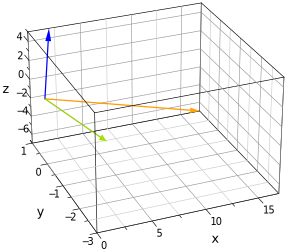
\includegraphics[width=0.5\linewidth]{mai_fig025.pdf}
    \captionof{figure}[Ortogonální doplněk]{Vizualizace vektorového prostoru a jeho    
             ortogonálního doplňku pomocí sw MatLab - MuPAD příkazem:\newline
             \texttt{plot(plot::Arrow3d([1,-3,2]), plot::Arrow3d([2,1,5]), 
             plot::Arrow3d([17,1,-7]))}}
    \label{LA:fig_ort01}
    \par}
\end{example}

      %---------------------------------------------------------------

      Výsledek předchozího příkladu \ref{mai:exam011} lze interpretovat tak, že jsme našli všechny 
      vektory, které jsou kolmé na rovinu určenou vektory ze zadání. Rovina je útvar       
      dvojrozměrný a protože prostor všech vektorů je trojrozměrný, musí nutně mít podprostor 
      ortogonálních vektorů ve shodě se vztahem \ref{LA:eq_dim_doplnek} pouze jednu dimenzi. Vše 
      je dobře patrné z obr. \ref{LA:fig_ort01}

  %=========================== Kapitola: Vlastní čísla a vlastní vektory ==========================
  \section{Vlastní čísla a vlastní vektory}\label{mai:IIchapIsecIII}
    \subsection{Motivace} 
      \textbf{Poznámka}: Je-li \(\mathcal{A} : \mathcal{V} \rightarrow \mathcal{V}\) lineární 
      zobrazení z prostoru \(\mathcal{V}\) do prostoru \(\mathcal{V}\) (nikdy se takové zobrazení 
      nazývá lineárním operátorem), pak je přirozeným požadavkem najít takovou bázi prostoru 
      \(\mathcal{V}\), že je matice zobrazení $\mathbf{A}$ v této bázi co nejjednodušší, např. má 
      následující strukturu
      \begin{equation*}
         \mathbf{A}=
           \left(\begin{array}{ccccc}
             \boxed{A_1}       &             &       &       & 0   \\
                 & \boxed{A_2} &             &       &             \\
                 &             & \boxed{A_3} &       &             \\
                 &             &             &\ddots &             \\
              0  &             &             &       & \boxed{A_k}
            \end{array}
           \right),
     \end{equation*}
     kde \(A_k\) jsou čtvercové matice malého řádu (nejlépe \(1\) nebo \(2\)) a ostatní prvky 
     matice jsou nulové. Problém najít bázi, aby v ní matice zobrazení měla diagonální tvar (kde 
     \(A_k\) jsou skaláry), vede k pojmu vlastní číslo a vlastní vektor matice.

      \begin{definition} 
        Nechť \(\mathbf{A}\in \mathcal{C}^{n,n}\) (matice je čtvercová řádu \(n\)).
        \begin{equation}
          \mathbf{A} = (a_{ij}) =
            \begin{pmatrix}
              a_{11} & a_{12} & \ldots & a_{1n} \\
              a_{21} & a_{22} & \ldots & a_{2n} \\
              \vdots & \vdots & \ddots & \vdots \\
              a_{n1} & a_{n2} & \ldots & a_{nn}
            \end{pmatrix}
        \end{equation}

        Jestliže platí
        \begin{equation}\label{eq:vl_number}
          \mathbf{Au} = \lambda\mathbf{u}
        \end{equation}
        pro jisté komplexní číslo \(\lambda\in\mathcal{C}\)  a jistý nenulový vektor 
        \(x\in\mathcal{C}^n, \mathbf{u}\neq\Theta\), potom číslo \(\lambda\) nazýváme 
        \textbf{vlastním číslem} matice \(\mathbf{A}\) a vektor \(\mathbf{u}\) \textbf{vlastním 
        vektorem} příslušným k tomuto vlastnímu číslu. Množinu všech vlastních čísel nazýváme 
        \textbf{spektrem matice} \(\mathbf{A}\). Pokud rov. \ref{eq:vl_number} rozepíšeme, dostaneme
        \begin{equation}
          \begin{pmatrix}
            a_{11} & a_{12} & \ldots & a_{1n} \\
            a_{21} & a_{22} & \ldots & a_{2n} \\
            \vdots & \vdots & \ddots & \vdots \\
            a_{n1} & a_{n2} & \ldots & a_{nn}
          \end{pmatrix}   \cdot
          \begin{pmatrix}
            u_{1} \\  u_{2} \\ \vdots \\  u_{n} \\
          \end{pmatrix}    =\lambda\cdot
          \begin{pmatrix}
            u_{1} \\ u_{2} \\ \vdots \\ u_{n} \\
          \end{pmatrix}
        \end{equation}
        můžeme ji rovněž psát ve tvaru
        \begin{equation*}
            \begin{pmatrix}
            \setlength{\arraycolsep}{3pt}
              a_{11} -\lambda & a_{12}           & \ldots & a_{1n} \\
              a_{21}          & a_{22} -\lambda  & \ldots & a_{2n} \\
              \vdots          & \vdots           & \ddots & \vdots \\
              a_{n1}          & a_{n2}           & \ldots & a_{nn}-\lambda
            \end{pmatrix} \cdot
          \begin{pmatrix}
            u_{1} \\ u_{2} \\ \vdots \\ u_{n} \\
          \end{pmatrix}  =
          \begin{pmatrix}
              0 \\ 0 \\ \vdots \\ 0 \\
            \end{pmatrix}
        \end{equation*}
      \end{definition}

       Tato soustava rov. je \textbf{homogenní} a stručně ji můžeme zapsat
      \begin{equation}\label{vv_hom_zapis}
        \left(\mathbf{A} - \lambda\mathbf{I}\right) = \mathbf{0}
      \end{equation}
      Homogenní soustava má \emph{netriviální řešení}, právě když je determinant matice soustavy 
      roven  nule, tj. v případě soustavy rov. rov. \ref{vv_hom_zapis} platí
      \begin{equation}\label{vv_hom_reseni}
        \abs{\mathbf{A} - \lambda\mathbf{I}} = \mathbf{0}
      \end{equation}
      Determinant \(A(\lambda)=\abs{\mathbf{A} - \lambda \mathbf{I}}\) nazýváme 
      \textbf{charakteristický polynom} matice \(\mathbf{A}\) - jedná se o polynom stupně \(n\) v 
      proměnné \(\lambda\), který má v oboru komplexních čísel \(n\) kořenů. Rovnici 
      \(A(\lambda)=0\) nazýváme \textbf{charakteristická rovnice matice \(\mathbf{A}\)} - jejími 
      kořeny jsou \textbf{charakteristické hodnoty} (resp. \textbf{vlastní čísla}) 
      \textbf{matice} \(\mathbf{A}\).
            
      \begin{tcnote}
        U vlastních čísel studium pouze reálných matic ztrácí smysl, protože i 
        reálná matice může mít komplexní vlastní čísla. Proto se uvažuje obecná komplexní matice.
      \end{tcnote}
      
      \begin{tcnote}
        Podmínka existence nenulového vektoru \(\mathbf{u} = \Theta\) v definici 
        vlastního čísla je nezbytná: kdyby bylo připuštěno i \(\mathbf{u} = \emptyset\), potom by 
        každé komplexní číslo bylo vlastním číslem a definice by ztratila smysl.
      \end{tcnote}
      
      \begin{tcnote}
        Odpovídá-li matice \(\mathbf{A}\) matici nějakého zobrazení \(\mathcal{A}\), pak každý 
        nenulový vektor z jádra zobrazení \(\ker\mathcal{A}\) je vlastním vektorem příslušným 
        vlastnímu číslu \(\lambda\). Je-li \(\ker\mathcal{A} = \{\Theta\}\) 
        (je-li matice \(\mathbf{A}\) regulární), pak \(\Theta\) není vlastním číslem matice 
        \(\mathbf{A}\).
      \end{tcnote}

      %---------------------------------------------------------------
        % !TeX spellcheck = cs_CZ
\begin{mathexam}{Ortogonální projekce v prostoru \(\mathcal{R}^3\)}{exam012}
    Je-li \(\mathbf{P}\) matice ortogonální projekce v prostoru \(\mathcal{R}^3\) na nějaký 
    podprostor \(\mathcal{U}\) (\(\mathcal{U}\) je tedy buď rovina nebo přímka procházející 
    počátkem), pak pro každý vektor \(\mathbf{u}\in\mathcal{U}\) platí \(\mathbf{Pu} = 
    \mathbf{u}\), všechny vektory z \(\mathcal{U}\) (s výjimkou nulového vektoru \(\Theta\)) 
    jsou vlastními vektory matice $\mathbf{P}$ příslušné vlastnímu číslu \(\lambda\). Prostor 
    \(\mathrm{U}^\bot\) je roven jádru projekce (nulovému prostoru matice \(\mathbf{P}\)), 
    a tedy každý vektor z ortogonálního doplňku \(\mathcal{U}\) (s výjimkou \(\Theta\)) je 
    vlastním vektorem příslušným k vlastnímu číslu \(0\).

    {\centering
      \captionsetup{type=figure}
      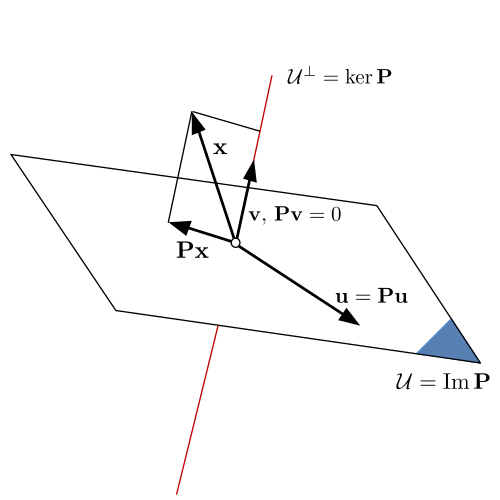
\includegraphics[width=0.5\linewidth]{mai_fig024.pdf}
      \captionof{figure}{K příkladu \ref{mai:exam012}}
      \label{MAI:FIG016}
      \par}

\end{mathexam}
      %---------------------------------------------------------------

      %---------------------------------------------------------------
        % !TeX spellcheck = cs_CZ


\begin{example}\label{mai:exam013}
  Určete spektrum matice a její spektrální poloměr následující matice
    \begin{equation*}\label{pr:spektrum_matice}
      \mathbf{A} =
        \begin{pmatrix}
          2  &  2    & 0 \\
         -3  & -3    & 5 \\
          0  & -0.25 & 2
        \end{pmatrix}
    \end{equation*}
  \textbf{Řešení}: Spektrum matice je množina všech jejích vlastních čísel. Spektrální poloměr 
  je maximum z absolutních hodnot vlastních čísel. Vlastní čísla určíme z charakteristické
  rovnice \(\det(\mathbf{A}-\lambda \mathbf{I})=0\).
    \begin{equation*}
      \textbf{A} - \lambda\textbf{I}=
        \begin{pmatrix}
          2-\lambda  &  2          & 0 \\
         -3          & -3-\lambda  & 5 \\
          0          & -0.25       & 2-\lambda
       \end{pmatrix}
    \end{equation*}
    \begin{align}
      \det(\mathbf{A}-\lambda \mathbf{I})                    &= 0           \nonumber\\
      (2-\lambda)
        \begin{pmatrix}
          -3-\lambda  &  5\\
             -0.25    &  2 - \lambda
        \end{pmatrix} -2\cdot
        \begin{pmatrix}
          -3       &  5\\
           0       &  2 - \lambda
        \end{pmatrix}                                        &= 0           \nonumber\\
      (2-\lambda)^2(-3-\lambda)+1.25(2-\lambda)+6(2-\lambda) &= 0           \nonumber\\
      (2-\lambda)[(2-\lambda)(-3-\lambda)+1.25+6]            &= 0           \nonumber\\
      (2-\lambda)(\lambda^2+\lambda+1.25)                    &= 0           \nonumber
    \end{align}
    \begin{equation*}
      \lambda_1 = 2, \quad\lambda_2 = -0.5+i, \quad\lambda_3=-0.5-i
    \end{equation*}
    \begin{itemize}
      \item Spektrum matice \(\mathbf{A}\) je \(\sigma(\mathbf{A})=\{2,-0.5+i,-0.5-i\}\).
      \item Spektrální poloměr \(\rho(\mathbf{A})=\max_i|\lambda_i|=2\).
    \end{itemize}

%    \attachfile[icon=Paperclip, description=Matlab Determine the spectrum of a matrix 
%      and its spectral radius]{../SRC/MAI/matlab/LA001.m}

\end{example}
      %---------------------------------------------------------------

      %---------------------------------------------------------------
        % !TeX spellcheck = cs_CZ
\begin{example}\label{mai:exam014}
  Určete vlastní čísla a vlastní vektory matice \(\mathbf{B} = \mathbf{A}^2 - 4\mathbf{A} + 
  9\mathbf{A}^{-1} - \mathbf{I}\), kde \(\mathbf{A}\) je matice \(\mathbf{A}= 
  \begin{pmatrix}1&0.5\\3.5&4\end{pmatrix}\).

  \textbf{Řešení}: (z předchozího příkladu víme, že \(\lambda_1=4.5, \lambda_2=0.5\)) a
   \(\mathbf{I}\) jednotková matice. Označme symbolem \(\lambda\) vlastní číslo matice 
   \(\mathbf{A}\) a nechť \(\mathbf{x}\) je příslušný vlastní vektor. Pak platí:
   \begin{itemize}
     \item Matice \(\mathbf{A}^2\) má vlastní čísla rovna \(\lambda^2\).
     \item Matice \(4\mathbf{A}\) má vlastní čísla rovna \(4\lambda\).
     \item Matice \(9\mathbf{A}^{-1}\) má vlastní čísla rovna \(\frac{9}{\lambda}\).
   \end{itemize}
   Matice \(\mathbf{B}=\mathbf{A}^2-4\mathbf{A}+9\mathbf{A}^{-1}-\mathbf{I}\) má vlastní čísla 
   ve tvaru  \(\lambda^2-4\lambda+\frac{9}{\lambda}-1\), vlastní vektory jsou stejné jako 
   vlastní vektory odpovídající vlastním číslům matice \(\mathbf{A}\). Tedy:
   \begin{equation*}
       \sigma(B)=\{4.5^2-4\cdot4.5+\frac{9}{4.5}-1,\quad
       0.5^2-4\cdot0.5+\frac{9}{0.5}-1\}=\{3.25, 15.25\}
   \end{equation*}
\end{example}
      %---------------------------------------------------------------


      %---------------------------------------------------------------
       % !TeX spellcheck = cs_CZ
\begin{mathexam}{Určete vlastní čísla a odpovídající vlastní vektory následují\-cích matic:
  \begin{equation*}
    \mathbf{A}=
      \begin{pmatrix}
        1   & 0.5\\
        3.5 & 4
      \end{pmatrix}, \quad
    \mathbf{B}=
      \begin{pmatrix}
        3   & -1 \\
        2.5 &  4 
      \end{pmatrix}
  \end{equation*}
  }{exam002}

  Vlastní čísla určíme z charakteristické rovnice: \(\det(\mathbf{A} - \lambda\mathbf{I}) = 0\).
  Vlastní vektory \(\mathbf{x_i}\) odpovídající vlastním číslům \(\lambda_i\), jsou řešením
  homogenní soustavy rovnic \((\mathbf{A} - \lambda_i\mathbf{I})\mathbf{x_i} = 0\).
  \begin{itemize}
    \item Vlastní čísla matice \textbf{A}:
      \begin{equation*}
          \textbf{A} - \lambda\textbf{I} =
            \begin{pmatrix}
                1-\lambda  &  0.5          \\
              -3.5         &  4-\lambda
            \end{pmatrix}
      \end{equation*}
      \begin{align*}
        \det(\mathbf{A}-\lambda\mathbf{I}) &= 0 \\
        (1-\lambda)(4-\lambda)-\frac{7}{4} &= 0 \\
        \lambda^2-5\lambda+\frac{9}{4}     &= 0
      \end{align*}
      \begin{equation*}
        \lambda_1 = 4.5,\quad \lambda_2 = 0.5
      \end{equation*}
  \end{itemize}

  \begin{itemize}
    \item Vlastní čísla matice \textbf{B}:
      \begin{equation*}
          \textbf{B} - \lambda\textbf{I}=
            \begin{pmatrix}
              3-\lambda  & -1             \\
              2.5        &  4-\lambda
            \end{pmatrix}
      \end{equation*}
      \begin{align*}
        \det(\mathbf{B}-\lambda\mathbf{I}) &= 0 \\
        (3-\lambda)(4-\lambda)+\frac{5}{2} &= 0 \\
        \lambda^2-7\lambda+\frac{29}{2}    &= 0
      \end{align*}
      \begin{equation*}
        \lambda_1 = \frac{7+3i}{2},\quad \lambda_2 = \frac{7-3i}{2}
      \end{equation*}
  \end{itemize}
  % matice A
  Vlastní vektor matice \(\mathbf{A}\) pro \(\lambda_1=4.5: (\mathbf{A} -
  \lambda_1\mathbf{I})\mathbf{x_1} = 0 \Rightarrow\)
  \begin{equation*}
    \begin{pmatrix}
      1  -4.5  &  0.5     \\
      -3.5     &  4-4.5
    \end{pmatrix}
    \sim
    \begin{pmatrix}
      -3.5  &  0.5         \\
      -3.5  & -0.5
    \end{pmatrix}
  \end{equation*}
  \begin{equation*}
    \Rightarrow\mathbf{x_1} =
    \begin{pmatrix}
      1 \\ 7
    \end{pmatrix}
    \, r, r\in\mathbb{R}, r\neq0
  \end{equation*}
  Vlastní vektor matice \(\mathbf{A}\) pro \(\lambda_2=0.5: (\mathbf{A} -
  \lambda_1\mathbf{I})\mathbf{x_2}=0 \Rightarrow\)
  \begin{equation*}
    \begin{pmatrix}
      1  -0.5  &  0.5   \\
      -3.5      &  4-0.5
    \end{pmatrix}
    \sim
    \begin{pmatrix}
      0.5  &  0.5       \\
      3.5  &  3.5
    \end{pmatrix}
  \end{equation*}
  \begin{equation*}
    \Rightarrow\mathbf{x_2} =
    \begin{pmatrix}
      -1 \\ 1
    \end{pmatrix}
    \, r, r\in\mathbb{R}, r\neq0
  \end{equation*}
  % matice B
  Vlastní vektor matice \(\mathbf{A}\) pro \(\lambda_1=\frac{7+3i}{2}: (\mathbf{B} -
  \lambda_1\mathbf{I})\mathbf{x_1}=0 \Rightarrow\)
  \begin{align*}
    \begin{pmatrix}
      3 - \frac{7+3i}{2}            & -1                                       \\
      \frac{5}{2}                   &  4 - \frac{7+3i}{2}
    \end{pmatrix}
    &\sim
    \begin{pmatrix}
      -\frac{1}{2}-\frac{3}{2}i      &  -1                                     \\
      \frac{5}{2}                    & \frac{1}{2}-\frac{3}{2}i
    \end{pmatrix}
    \sim                                                                            \\
    \begin{pmatrix}
      -\frac{10}{4}                  &-\left(\frac{1}{2} -\frac{3}{2}i\right)  \\
      \frac{5}{2}                    & \frac{1}{2}-\frac{3}{2}i
    \end{pmatrix}
    &\sim
    \begin{pmatrix}
      -5                           &-\left(1-3i\right)                         \\
        5                           & \left(1-3i\right)
    \end{pmatrix}
  \end{align*} 
  \begin{align*} 
    \Rightarrow \mathbf{x_1}=
    \begin{pmatrix}
      -1+3i \\ 5
    \end{pmatrix}
    \, r, r\in\mathbb{C}, r\neq0
  \end{align*}
  Vlastní vektor matice \(\mathbf{B}\) pro \(\lambda_2=\frac{7-3i}{2}: (\mathbf{B} -
  \lambda_1\mathbf{I})\mathbf{x_2}=0 \Rightarrow\)
  \begin{align*}
    \begin{pmatrix}
      3  - \frac{7-3i}{2}       &  -1                                     \\
      \frac{5}{2}               &  4 - \frac{7-3i}{2}
    \end{pmatrix}
    &\sim
    \begin{pmatrix}
      -\frac{1}{2}+\frac{3}{2}i  &  -1                                     \\
      \frac{5}{2}                & \frac{1}{2}+\frac{3}{2}i
    \end{pmatrix}                                 
    \sim                                                                          \\
    \begin{pmatrix}
      -\frac{10}{4}              &-\left(\frac{1}{2} +\frac{3}{2}i\right)  \\
      \frac{5}{2}                & \quad\frac{1}{2}+\frac{3}{2}i
    \end{pmatrix}
    &\sim                                                                   
    \begin{pmatrix}
      -5                         &-\left(1+3i\right)                       \\
      5                          & \quad\left(1+3i\right)
    \end{pmatrix}
  \end{align*} 
  \begin{equation*} 
    \Rightarrow \mathbf{x_2}=
    \begin{pmatrix}
      -1-3i \\ 5
    \end{pmatrix}
    \, r, r\in\mathbb{C}, r\neq0
  \end{equation*}
  %---------------------------------------------------------------
  \lstinputlisting[%
    style=luaMatlabStyle,
    caption={Výpis programu pro ověření výpočtu vlastních čísel matic programem Matlab.}
    ]{../src/MAI/matlab/LA001.m}
  %--------------------------------------------------------------- 
\end{mathexam}
      %---------------------------------------------------------------


%--------------------------------------------------------------------------------------------------- 
%  % !TeX spellcheck = cs_CZ
%---------------------------------------------------------------------------------------------------
% mai2ch02.tex
%---------------------------------------------------------------------------------------------------
\setchaptertoc
\chapter{Souřadnicové soustavy obvyklejší i méně obvyklé}\label{mai:IIchapII}


%---------------------------------------------------------------------------------------------------
%  % !TeX spellcheck = cs_CZ
%---------------------------------------------------------------------------------------------------
% mai2ch03.tex
%---------------------------------------------------------------------------------------------------
\chapter{Linearita v aplikacích aneb lineární algebra do třetice}\label{mai:IIchapIII}
\minitoc

%---------------------------------------------------------------------------------------------------
\printbibliography[title={Seznam literatury}, heading=subbibliography]
\addcontentsline{toc}{section}{Seznam literatury}
%  % !TeX spellcheck = cs_CZ
%---------------------------------------------------------------------------------------------------
% mai2ch04.tex
%---------------------------------------------------------------------------------------------------
\setchaptertoc
\chapter{Obyčejné diferenciální rovnice}\label{mai:IIchapIV}

  V partii \ref{part:MAI} jsme se seznámili s funkcemi, o jejich užitečnosti nepochybujeme, neboť
  jsme se již přesvědčili, že se s nimi setkáváme takřka na každém kroku. Vyjadřují totiž
  jednoduchým způsobem vzájemnou souvislost veličin, a nejen fyzikálních. Známe-li například funkci
  vyjadřující závislost polohy tělesa na čase, můžeme zjistit, kde těleso v daném okamžiku bylo, je,
  nebo bude. Známe-li funkce, které popisuji časový vývoj cen a platů, můžeme snadno zjistit, zda za
  stejný peníz, za který dnes dostaneme deset housek, koupíme za rok dvacet, nebo jen dvě. Příroda,
  a ani ekonomika či politika, však nejsou natolik průhledné, aby nám takové závislosti předestřely
  přímo. Poskytují pouze informace o jejich změnách, a to ještě ukryté ve speciálních rovnicích,
  zvaných \emph{diferenciální}. Jde-li o neznámou reálnou funkci nebo soubor funkcí závislých na
  jedné reálné proměnné, třeba na čase, hovoříme o obyčejných diferenciálních rovnicích. Přesněji
  řečeno, diferenciální rovnice vyjadřuje matematickou formou zákon platný pro hledanou funkci a
  její derivace prvního nebo i vyšších řádů. Takovou funkcí času může být například i množství látky
  při chemických reakcích, mohutnost populace živočichů, kurz eura, cena akcií na burze, rychlost
  pohybu těles, teplota atd. Ve fyzice a chemii jsou diferenciální rovnice dány fyzikálními či
  chemickými zákony, v ekonomii nebo biologii se objevují v různých modelech, odpovídajících více či
  méně skutečnosti. Uveďme si několik příkladů, na nichž si vysvětlíme základní terminologii, která
  je s problematikou diferenciálních rovnic spojena.
  
  Doplňková literatura pro studium této partie je například: \cite[s.~217]{Musilova2012MA2} a 
  \cite[s.~426]{Brabec1989}. Pro procvičení elementárních metod řešení konkrétních rovnic je vhodná 
  sbírka řešených příkladů \cite[s.~348]{Jirasek1989}.
  
  %--Příklad s hlemýžděm------------------------------------------
      % !TeX spellcheck = cs_CZ
% Musilova2009MA2
\begin{mdframed}[style=mdexam]
  \begin{example}\label{mai:exam084}
    \textbf{Pohyb po přímce}\newline
    Hlemýžď se pohybuje po přímce od kopretiny k pampelišce stálou rychlostí \(v_0 =
    \SI{2}{\mm\per\s}\). V počátečním okamžiku \(t = 0\) byl ve vzdálenosti \(s_0 = \SI{10}{\mm}\)
    od kopretiny. Jaká bude jeho vzdálenost od kopretiny v libovolném okamžiku \(t\geq0\)? Na tuto
    otázku by jistě snadno odpověděl i žák první třídy. Ukažme si však, že úlohu lze také vyjádřit
    pomocí diferenciální rovnice. Vzdálenost \(s(t)\) je hledanou funkcí jedné proměnné, a to času
    \(t\). Rychlost \(v_0\) rovnoměrného přímočarého pohybu je časovou derivací vzdálenosti.
    Získáváme tedy rovnici

    {\centering
     \captionsetup{type=figure}
     \luafigure[0.7]{mai_fig055.png}
     \captionof{figure}{Hlemýžď pohybující se po přímce od kopretiny k pampelišce 
                       \cite[s.~217]{Musilova2012MA2}}
     \label{mai:fig055}
    \par}
    
    \begin{equation}\label{mai:eq076}
      \der{s(t)}{t} = v_0.
    \end{equation}

    Již jsme se zmínili, že rovnice obsahující neznámou reálnou funkci jedné reálné proměnné a její
    derivace obecně i vyššího řádu se nazývá obyčejnou diferenciální rovnicí. Každá z funkcí, které
    rovnici splňují, se nazývá jejím řešením. Řád rovnice je určen nejvyšší derivací, která se v
    rovnici vyskytuje, v našem příkladu jde tedy o rovnici prvního řádu.

    {\centering
     \captionsetup{type=figure}
     \luafigure[1]{mai_fig054.png}
     \captionof{figure}{Graf řešení počáteční úlohy (\ref{mai:eq077}).}
     \label{mai:fig054}
    \par}
    
    Řešení rovnice (\ref{mai:eq076}) snadno \uv{uhodneme}. Bude jím každá funkce
    \begin{equation*}
      s(t) = v_0t +C,
    \end{equation*}
    kde \(C\) je libovolné reálné číslo. Funkce, které jsou řešením rovnice, mají stejný charakter a
    jsou odlišeny pouze číselnou hodnotou \(C\), tvoří soubor, který se nazývá \textbf{obecné řešení
    rovnice}. Ze všech funkcí, které vyhovují rovnici (\ref{mai:eq076}), však skutečný pohyb
    hlemýždě popisuje právě jedna. Abychom ji našli, potřebujeme určit správnou hodnotu \(C\). K
    jejímu zjištění stačí, abychom věděli, jaká byla poloha hlemýždě v jediném okamžiku. Jestliže
    jsme například začali měřit čas ve chvíli, kdy byl hlemýžď ve vzdálenosti \(s_0\) od kopretiny,
    máme tzv. \textbf{počáteční podmínku} \(s(0) = s_0\). Pomocí ní můžeme z nekonečně mnoha funkcí
    obecného řešení vybrat jediné \textbf{partikulární řešení}. V našem případě to bude funkce
    \(s(t) = v_0t + s_0\). Naše rovnice společně s počáteční podmínkou, tj.
    \begin{equation}\label{mai:eq077}
      \der{s(t)}{t} = v_0, \qquad s(0) = s_0,
    \end{equation}
    představuje tzv. \textbf{počáteční úlohu}. Její řešení je v grafu na obrázku \ref{mai:fig054}
    vyznačeno červeně, modře jsou vyznačena některá další partikulární řešení. Dokážete určit, jaké
    počáteční úloze odpovídají?
  \end{example}
\end{mdframed}
  %---------------------------------------------------------------
  Ve většině příkladů, se kterými se setkáme, bude mít počáteční úloha právě jedno řešení, jak tomu
  je v případě hlemýždě. Jestliže je nějaká funkce, definovaná na intervalu \((a,b)\), řešením
  počáteční úlohy, pak každá funkce, kterou vytvoříme zúžením původního řešení na „menší“ interval,
  bude opět rovnici splňovat. My však máme \emph{„právě jedním řešením“} na mysli tzv. \textbf{úplné
  řešení}, tj. takové, které není zúžením žádného jiného, a tak řešení lišící se pouze definičním
  oborem nebudeme považovat za odlišná. Jak uvidíme později, vyskytnou se však také příklady, kdy
  počáteční úloha nemá žádné řešení, nebo jich má naopak nekonečně mnoho.

  %--Příklad s koupelnou------------------------------------------
      % !TeX spellcheck = cs_CZ
% Musilova2009MA2
\begin{mdframed}[style=mdexam]
  \begin{example}\label{mai:exam085}
    \textbf{Příklad s koupelnou}\newline
      V koupelně o celkovém objemu \(V = \num{12000}\) litrů byl nainstalován větrák, jehož výkon je
      \(P = \num{400}\) litrů za minutu. Položme si otázku: Jaká je optimální doba, na kterou je
      třeba nastavit časový spínač, aby větrák neběžel příliš dlouho a přitom se vyměnil všechen
      vzduch v místnosti? A je to vůbec možné? Může se opravdu vzduch vyměnit všechen? Přemýšlejme o
      této situaci důkladněji. Označme \(c(t)\) funkci popisující okamžitou objemovou koncentraci
      „původního vzduchu“ v místnosti, tj. poměr objemu původního vzduchu ku objemu místnosti. (V
      okamžiku zapnutí větráku, tj. pro \(t = 0\), je \(c(0) = c_0 = 1\), v okamžiku, kdy bude
      původní vzduch zcela vyčerpán, pokud to vůbec nastane, bude \(c = 0\).) V intervalu \([t,t +
      \Delta t]\) větrák odčerpá \(P\Delta t\) litrů vzduchu celkem, z toho množství starého vzduchu
      činí \(c(t)P\Delta t\) a jeho podíl na celkovém množství vzduchu je \(c(t)P\Delta t/V\). Tato
      hodnota představuje pro velmi malé \(\Delta t\) \textbf{úbytek} koncentrace starého vzduchu v
      koupelně v časovém intervalu \([t, t + \Delta t]\), tj.
      \begin{equation*}
        \Delta c(t) = - \frac{c(t)P\Delta t}{V} \Rightarrow 
        \dfrac{\Delta c(t)}{\Delta t} = - \dfrac{P}{V}c(t)
      \end{equation*}
      
      (uměli bychom vysvětlit záporné znaménko?). Získáváme rovnici
      \begin{equation}\label{mai:eq078}
        \der{c(t)}{t} = - \dfrac{P}{V}c(t)
      \end{equation}
      Dosazením snadno ověříme, že řešením rovnice (\ref{mai:eq078}) je každá funkce
      \begin{equation*}
        c(t) = Ke^{-\frac{Pt}{V}},
      \end{equation*}

      {\centering
      \captionsetup{type=figure}
      \luafigure[1]{mai_fig056.png}
      \captionof{figure}{Graf řešení úlohy s koupelnou.}
      \label{mai:fig056}
      \par}
      
      kde \(K\) je libovolné číslo. Jeho konkrétní hodnotu pro náš případ určíme z počáteční
      podmínky \(c(0) = 1\), tj. \(K = 1\). A vida, pokud jsme počítali správně, můžeme usoudit, že
      koncentrace původního vzduchu neklesne na nulovou hodnotu nikdy. Naše řešení samozřejmě
      nevylučuje použití časového spínače - rozumně bychom mohli například požadovat, aby
      koncentrace původního vzduchu klesla na hodnotu \(c(\tau) = \num{0.1}\). Hledaná doba bude \(t
      =\frac{P}{V}\ln(1/c(\tau)) =\qty{69}{\minute}\). Řešení naší počáteční úlohy je v grafu na
      obrázku \ref{mai:fig056} vyznačeno červeně. Jakým počátečním úlohám odpovídají modré křivky?
  \end{example}
\end{mdframed}
  %---------------------------------------------------------------
  
  \begin{tcnote}
    „Větrací“ rovnice, diskutovaná v předchozím případě, se ve fyzice objevuje poměrně často. Někdy
    je nazývána lineárním diferenciálním zákonem. Narazíme na ni vždy, když je rychlost změny nějaké
    veličiny (její první derivace) přímo úměrná veličině samotné. Tak například při rozpadu
    radioaktivních jader dospějeme k rovnici \(\der{N(t)}{t} = -\lambda N(t)\), kde \(N(t)\) je
    počet radioaktivních jader ve vzorku v okamžiku \(t\) a \(\lambda\) je \textbf{rozpadová
    konstanta}. Při zkoumání absorpce rentgenového záření v látce získáme rovnici \(\der{I(x)}{x} =
    -\mu I(x)\), kde \(I(x)\) je intenzita v hloubce \(x\) pod povrchem a \(\mu\) je lineární
    \textbf{koeficient absorpce}. S oběma příklady jsme se již setkali v partii \ref{part:MAI}.
    Zkusme si vzpomenout na další příklady lineárních diferenciálních zákonů.
  \end{tcnote}

  %--Příklad o sáňkování------------------------------------------
      % !TeX spellcheck = cs_CZ
% Musilova2009MA2
\begin{mdframed}[style=mdexam]
  \begin{example}\label{mai:exam086}
    \textbf{Příklad o sáňkování}\newline
    Kdo bude rychlejší na sáňkách? Tatínek o hmotnosti \(M\), nebo Pepíček s Mařenkou o hmotnosti
    \(m\)? Každý fyzik hned namítne, že tíhové zrychlení, které určuje rozjezd sáněk, na hmotnosti
    nezávisí. Z praxe však víme, že tatínkové bývají rychlejší. Jak to? Zřejmě proto, že sáňkování
    ve vakuu není obvyklé. Kromě průmětu tíhové síly do nakloněné roviny (\(F_1 = Mg\sin\alpha\)),
    který „nás urychluje", jsme brzděni silou odporu prostředí. V jednoduchém přiblížení ji můžeme
    předpokládat ve tvaru \(F_2 = -Cv^2\). Konstanta \(C\) závisí na tvaru a rozměrech pohybujícího
    se objektu a na hustotě vzduchu. Pro jednoduchost předpokládáme, že je stejná u tatínka i
    Pepíčka. Fyzikální zákon \(Ma= F_1 + F_2 = Mg\sin\alpha - Cv^2\)

    {\centering
    \captionsetup{type=figure}
    \luafigure[1]{mai_fig057.jpg}
    \captionof{figure}{Ladův obrázek dětí na sáňkách.}
    \label{mai:fig057}
    \par}

    například pro tatínka můžeme přepsat na diferenciální rovnici takto:
    \begin{equation}\label{mai:eq079}
      M\der{v}{t} = Mg\sin\alpha - Cv^2
    \end{equation}
    
    Hledanou funkcí je nyní časová závislost rychlosti, jako počáteční podmínku budeme uvažovat, že
    rychlost v čase \(t = 0\) byla nulová. Řešením této počáteční úlohy je funkce
    \begin{align*}
      v(t) &= \sqrt{\dfrac{Mg\sin\alpha}{C}}
              \left[\dfrac{e^{2t\sqrt{\dfrac{Cg\sin\alpha}{M}}}-1}
                          {e^{2t\sqrt{\dfrac{Cg\sin\alpha}{M}}}+1}
              \right]                                                                           \\
          &= \sqrt{\dfrac{Mg\sin\alpha}{C}}\tanh\left(t\sqrt{\dfrac{Cg\sin\alpha}{M}}\right).
    \end{align*}
    Graf takovéto závislosti pro dvě různé hmotnosti \(M = \SI{100}{\kg}\) (červená) a \(m =\SI{10}
    {\kg}\) (modrá) vidíme na obrázku \ref{mai:fig057}. (Poměr hmotností byl takto zvolen pro
    zvýraznění rozdílnosti výsledků - každému je zřejmé, že mimino samo sáňkovat nemůže.) Další
    hodnoty: \(\alpha = \ang{20}\), \(g = \SI{10}{\m\per\square\s}\), \(C =
    \SI{1.00}{N\m^2s^{-2}}\). Na obrázku \ref{mai:fig058} si všimněme, že rychlost se nejprve

    {\centering
    \captionsetup{type=figure}
    \luafigure[1]{mai_fig058.png}
    \captionof{figure}{Graf řešení úlohy o sáňkování. \cite[s.~221]{Musilova2012MA2}}
    \label{mai:fig058}
    \par}

    poměrně prudce zvyšuje, ale poté se asymptoticky blíží k tzv. \textbf{mezní rychlosti} \(v_{max}
    = Mg\sin\alpha\). Mezní rychlost odpovídá situaci, kdy se síly \(F_1\) a \(F_2\) „vyrovnají“.
    (Taková situace však nenastane, je pouze limitním případem pro \(t \rightarrow \infty\).) 
  \end{example}
\end{mdframed}
  %---------------------------------------------------------------
  \begin{tcnote}
    Zamysleme se také nad tím, jak jsme z vyjádření funkce \(v(t)\) pomocí exponenciálních funkcí 
    získali elegantnější výraz s hyperbolickou tangentou. Pro připomenutí hyperbolických funkcí se 
    můžeme vrátit k odstavci 2.1.8 partie \ref{part:MAI}.
  \end{tcnote}
  
  Na uvedených příkladech jsme se mohli přesvědčit, že porozumění některým realistickým dějům
  vyžaduje umět sestavit a řešit diferenciální rovnice. Problémy, se kterými se v životě setkáváme,
  však obvykle vedou k rovnicím mnohem komplikovanějším. Proto často používáme aproximací a skutečný
  svět si poněkud „idealizujeme". Tak například v úloze s koupelnou jsme předpokládali, že vzduch v
  místnosti je vždy dokonale promíchán, v úloze o sáňkování jsme pro odporovou sílu použili pouze
  přibližný zákon a zanedbali třecí sílu. Často se setkáme s rovnicemi, které dokážeme řešit pouze
  numerickými metodami za pomoci počítačů. Aproximativní přístupy tedy mohou vstupovat do popisu
  vývoje reálných systémů pomocí diferenciálních rovnic dvojím způsobem. Poprvé již při samotném
  sestavení diferenciálních rovnic, podruhé při jejich řešení.
  
  V této kapitole se budeme věnovat některým typickým situacím, kdy je možné získat řešení
  diferenciálních rovnic analytickými metodami, zjednodušeně řečeno „tužkou na papíře“. Proč se
  omezujeme na některé typické situace“? Protože problematika diferenciálních rovnic obsahuje ještě
  další úskalí. Řečeno s mírnou nadsázkou, existuje totiž nepřeberné množství různých typů
  diferenciálních rovnic, dokonce už v případě rovnic prvního řádu, které při řešení vyžadují takřka
  \uv{individuální přístup}. I když samozřejmě v teorii diferenciálních rovnic existuje řada
  obecných výsledků společných určité širší skupině diferenciálních rovnic, není možné formulovat
  nějaký \uv{univerzální} postup, který by vedl k řešení kterékoli z nich. V praxi je proto třeba
  naučit se rozpoznat jednotlivé typy obyčejných diferenciálních rovnic a zvolit pro jejich řešení
  vhodnou metodu. Ne nadarmo se proto textům o diferenciálních rovnicích říká „kuchařky“, aniž by to
  mělo hanlivý nádech. (Vznešenější slovo pro „kuchařku“ je „příručka“. Pokud jde o problematiku
  obyčejných diferenciálních rovnic, je takovou moderní příručkou kniha \cite{PolyaninZaitsev},
  která na více než osmi stech stran obsahuje přes 6 200 rovnic s řešeními!
  
  \twocolumn[\section{Diferenicální rovnice vyskytující se kolem nás}\label{mai:IIchapIVsecI}]
    V tomto odstavci jsou zařazeny motivační příklady ukazující, že diferenciální rovnice se
    skutečně objevují v různých vědních oborech. Rovnice jsou většinou uvedeny bez řešení, ale jsou
    doplněny alespoň odkazy ve kterých lze najít mnohem více informací, které jdou za rámec této
    partie o obyčených diferenciálních rovnicích. Stejně jako v předchozích příklad, řada
    fyzikálních principů má tvar výroku, resp. vztahu mezi jistými veličinami (funkcemi) a jejich
    změnami, vztaženými ke zvoleným nezávisle proměnným (pa\-ra\-me\-trům) (\emph{čas, souřadnice}).
    Je to přirozené, neboť (\emph{okamžité}, či \emph{okální}) změny se nejlépe vystihují pomocí
    derivací. Takový zákon má pak charakter vztahu mezi uvažovanými veličinami a jejich derivacemi. 
    
    \begin{tcnote}
      V matematických textech o obyčejných diferenciálních rovnicích se označuje nezávisle proměnná
      obvykle symbolem \(x\), neznámá funkce \(y = y(x)\) nebo \(y = f(x)\) a její derivace čárkami,
      tj. \(y'(x)\), \(y''(x)\) nebo \(y' = f'(x)\), \(y'' = f''(x)\) atd. V mnoha fyzikálních i
      jiných praktických situacích však bývá nezávisle proměnnou čas \(t\) a hledáme závislost
      veličiny \(x = x(t)\) na čase. Tohoto značení budeme velmi často používat, přičemž první,
      resp. druhou derivaci funkce \(x(t)\) budeme podle zvyklosti zavedené ve fyzice vyznačovat
      pomocí tečky, resp. dvou teček nad symbolem \(x\),
      \begin{equation*}
        \dot{x}(t) = \der{x}{t}, \qquad \ddot{x}(t) = \dder{x}{t}.
      \end{equation*}
      Pro větší přehlednost zápisu budeme často vynechávat argument \(t\) v závorce, \(\dot{x} = 
      \dot{x}(t)\). Nebudeli řečeno jinak, předpokládáme, že všechny funkce jsou spojité, případně 
      i diferencovatelné na celém svém definičním oboru nebo alespoň na jistém oboru, který je jeho 
      podmnožinou. Při práci s podílem funkcí budeme automaticky předpokládat, že jmenovatelem je 
      funkce, která je nenulová ve všech bodech uvažovaného intervalu.      
    \end{tcnote}
    
    \subsection{Diferenciální rovnice v mechanice}
      \textbf{Druhý Newtonův pohybový} zákon pro hmotný bod, který nabývá tvaru
      \begin{equation*}
        m\vec{a} = \vec{F}
      \end{equation*}
      skrývá soustavou \emph{tří diferenciálních rovnic druhého řádu}. Složky zrychlení \(\vec{a}(t)
      = (a_x(t), a_y(t), a_z(t)) = (\ddot{x}(t), \ddot{y}(t), \ddot{z}(t))\) jsou totiž druhými
      derivacemi složek polohového vektoru \(\vec{r}(t) = (x(t), y(t), z(t))\) podle času, vektor
      výslednice sil působících na hmotný bod je obecně funkcí jeho polohy a rychlosti, a často také
      explicitní funkcí času. Platí tedy \(\vec{F} = \vec{F}(\vec{r},\vec{v},t)\). Rozepíšeme-li
      druhý Newtonův zákon do složek, dostaneme
      \begin{align*}
        m\ddot{x} & = F_x(x,y,z,\dot{x}, \dot{y}, \dot{z}, t),        \\
        m\ddot{y} & = F_y(x,y,z,\dot{x}, \dot{y}, \dot{z}, t),        \\
        m\ddot{z} & = F_z(x,y,z,\dot{x}, \dot{y}, \dot{z}, t)
      \end{align*}
      Řešením této soustavy je časová závislost \(\vec{r} = (x(t), y(t), z(t))\) polohového vektoru
      hmotného bodu. Je \emph{parametrickým vyjádřenim křivky}, po které se hmotný bod v prostoru
      pohybuje, nazývá se \emph{trajektorií} pohybu.Zadáním počáteční polohy \(\vec{r}_0 = (x(t_0),
      y(t_0), z(t_0))\) a počáteční rychlosti \(v_0 = (\dot{x}(t_0), \dot{y}(t_0), \dot{z}(t_0))\)
      například v okamžiku \(t_0 = 0\) ziskáme \textbf{počáteční úlohu}. (Soustava obsahuje druhé
      derivace neznámých funkci \(x(t)\), \(y(t)\) a \(z(t)\), proto potřebujeme dvě podmínky pro
      každou z nich.) 
      
      Zapišme takový příklad konkrétní soustavy: Na planetu o hmotnosti \(m\) působí Slunce o
      hmotnosti \(M\) silou \(\vec{F}_g\) danou Newtonovým gravitačním zákonem. Tentokrát však jde o
      tzv. „silový zákon", který popisuje gravitační interakci planety a Slunce. Umístíme-li počátek
      soustavy souřadnic do hmotného bodu představujícího Slunce, platí
      \begin{equation*}
        \vec{F}_g = - \dfrac{\kappa mM\vec{r}}{r^3} 
                  = - \dfrac{\kappa mM}{(x^2+y^2+z^2)^{\frac{3}{2}}}(x, y, z)
      \end{equation*}
      kde \(\kappa =  \SI{6.67e-11}{\N\m^2\kg^{-2}}\) je jednou z univerzálních fyzikálních
      konstant, nazývanou gravitační konstanta. Za předpokladu, že zanedbáme pohyb Slunce a
      gravitační působení planet a ostatních těles, má soustava rovnic vyjadřující druhý Newtonův
      zákon pro planetu tvar 
      \begin{subequations}
        \begin{empheq}[box=\widefbox]{align*}
          m\ddot{x} & = - \kappa mM \dfrac{x}{(x^2+y^2+z^2)^{\frac{3}{2}}},        \\
          m\ddot{y} & = - \kappa mM \dfrac{y}{(x^2+y^2+z^2)^{\frac{3}{2}}},        \\
          m\ddot{z} & = - \kappa mM \dfrac{z}{(x^2+y^2+z^2)^{\frac{3}{2}}}
        \end{empheq}
      \end{subequations}

      Nalézt řešení této soustavy znamená „vydolovat" z ní, při daných počátečních podmínkách,
      konkrétní tvar funkcí \(x(t)\), \(y(t)\) a \(z(t)\). Zrovna tato úloha není příliš jednoduchá.
      Postup při jejím řešení, který lze usnadnit použitím fyzikálních \uv{triků}, si ukážeme později. 

    \subsection{Diferenciální rovnice v chemii}
      Uvažujme o chemické reakci, při které se ze dvou látek \(A\) a \(B\) syntetizuje látka \(C\).
      Na jeden gram výsledné látky je zapotřebí \(p\) gramů látky \(A\) a \(1 - p\) gramů látky
      \(B\). Smícháme \(a\) gramů látky \(A\) s \(b\) gramy látky \(B\). Na počátku je hmotnost
      látky \(C\) nulová, její hodnotu v čase \(t\) označíme \(x(t)\). Rychlost chemické reakce, tj.
      změna hmotnosti látky \(C\) s časem, je v rámci nejjednoduššího modelu rovna veličině \((a -
      px) (b - (1 - p)x)\). Vidíme, že při zvětšujícím se množství výsledné látky bude rychlost
      reakce klesat. Ve výsledku se projeví i to, jaké množství výchozích látek smícháme, resp. jak
      se jejich poměr \(\dfrac{a}{b}\) bude lišit od „ideálního" poměru \(\dfrac{p}{1-p}\). Rovnice
      popisující reakci je diferenciální rovnicí prvního řádu pro časovou závislost \(x(t)\)
      hmotnosti látky \(C\)
      \begin{equation*}
        \boxed{\dot{x} = (a - px)(b - (1-p)x)}\, ,
      \end{equation*}
      s počáteční podmínkou \(x(0) = 0\). K této rovnici se ještě hodí poznamenat, že je příkladem
      (i když velmi speciálním) známé \textbf{Riccatiovy rovnice}, která má uplatnění i v
      praktických disciplínách, například v elektrotechnice nebo v oblasti automatického řízení.
      Přestože má nevinně vypadající obecný tvar \(x(t) = h(t) + f(t)x +g(t)x^2\), \(h(t) \neq 0\),
      \(g(t) \neq 0\), je tak trochu „zrádná“. Její řešení se totiž nemusí podařit zapsat pomocí
      elementárních funkcí. 
    
    \subsection{Diferenciální rovnice v biologii}
      Uvažujme o vlkovi a zajíci. Předpokládáme-li, že zajíc má vždycky co žrát (trávy je všude
      dost), bude nárůst počtu zajíců úměrný jejich okamžitému počtu (čím více je zajíců, tím více
      dalších se narodí). Zároveň jsou zajíci požíráni vlky a jejich úbytek je úměrný jak počtu
      vlků, tak počtu jich samých (čím více je zajíců, tím více jich každý věčně hladový vlk chytí a
      sežere, čím více je vlků, tím více zajíců sežerou). Co se vlků týče, ty nikdo nesežere, ale
      budou umírat hladem, jestliže nebude dostatek zajíců. Nárůst počtu vlků je tedy úměrný jak
      počtu vlků, tak počtu zajíců, kdežto úbytek je úměrný pouze počtu vlků. Získáváme soustavu
      dvou diferenciálních rovnic

      \begin{subequations}
        \begin{empheq}[box=\widefbox]{align*}
          \dot{z} &= \alpha z - \beta zv,     \\
          \dot{v} &= \gamma v + \delta zv,
        \end{empheq}
      \end{subequations}

      kde funkce \(z(t)\) resp. \(v(t)\) vyjadřují časovou závislost počtu zajíců, resp. vlků.
      Konstanty \(\alpha\), \(\beta\), \(\gamma\), \(\delta\) lze určit dlouhodobým pozorováním. 
      \begin{tcnote}
        Pokud někoho napadlo, že zajíci i vlci se také rodí i umírají „přirozenou cestou“, má
        pravdu. Tato skutečnost je v našem jednoduchém modelu zahrnuta. Přirozený přírůstek či
        úbytek zajíců i vlků je také úměrný jejich okamžitému počtu, a je tedy respektován
        empirickými hodnotami \(\alpha\), \(\gamma\).
      \end{tcnote}
      
      Tato soustava nelineárních diferenciálních rovnic se nazývá \textbf{Lotkova-Volterrova}. 
      Existence triviálního, tj. identicky nulového řešení, odpovídajícího situaci, kdy žádný zajíc 
      ani vlk neexistují je zřejmá na první pohled. Rovnice má však také netriviální řešení, které 
      si později ukážeme. 
      
      Obdobným příkladem z biologie je situace, kdy diferenciální rovnice popisuje časový průběh
      vývoje jedné populace. Řekněme, že jde o populaci bakterií, jejíž velikost v závislosti na
      čase je dána funkcí \(P(t)\). Při vývoji hrají roli dva nezávislé faktory, jeden způsobuje
      růst populace a druhý souvisí s omezeními danými prostředím. Představme si situaci tak, že bez
      omezujících vlivů prostředí by populace narůstala podle lineárního diferenciálního zákona, tj.
      derivace \(\dot{P}(t)\) hledané funkce \(P(t)\) by byla v každém okamžiku přímo úměrná hodnotě
      \(P(t)\), konstantu úměrnosti \(R\) nazvěme \emph{faktorem růstu}. Okolní prostředí však
      znemožňuje neomezené narůstání funkčních hodnot \(P(t)\). Růst je totiž modifikován tak, že se
      anuluje v okamžiku, kdy je dosaženo \uv{povolené} hodnoty \(P_{max} = K\), tj. když hodnota
      funkce \(P(t)\) dosáhne úrovně \emph{nosné kapacity} \(K\). Odpovídající diferenciální rovnice
      je opět nelineární a zní
      \begin{equation*}
        \boxed{\dot{P} = RP\left(1 - \dfrac{P}{K}\right)}
      \end{equation*}
      Nazýváme ji \textbf{logistickou rovnicí} a rovněž se ji naučíme vyřešit.
      
    \subsection{Diferenciální rovnice v ekonomii}
      V novinách se občas objeví zpráva, že míra inflace klesá. Od obyvatelstva se očekává, že to
      bude interpretovat jako pozitivní jev v naší ekonomice. Je tomu tak skutečně? Označme jako
      \(h(t)\) funkci popisující vhodným způsobem „kupní sílu“ koruny v závislosti na čase (název
      funkce \(h(t)\) jsme dali do uvozovek, neboť skutečná situace je z pohledu ekonomiky
      složitější a nezávisí pouze na inflaci). Její záporně vzatou derivaci \(\mu = -\der{h(t)}{t} =
      -h\) nazýváme mírou inflace. Proč znaménko minus? Pokud je funkce \(h(t)\) klesající, tj.
      kupní síla peněz se snižuje, je její derivace záporná. O míře inflace se však při znehodnocení
      kupní síly hovoří jako o kladné veličině. Jestliže míra inflace podle novinářů klesá, je její
      derivace \(\mu(t)\) záporná. Předpokládejme pro jednoduchost, že velikost této derivace je
      stálá. Druhá derivace neznámé funkce \(h(t)\) je tedy kladná konstantní hodnota, označme ji
      třeba \(A\), \(A > 0\). Dostáváme velmi jednoduchou diferenciální rovnici
      \begin{equation*}
        \ddot{h} = A.
      \end{equation*}
      kterou můžeme okamžitě vyřešit. Vyhovují jí všechny funkce tvaru
      \begin{align*}
        h(t) &= \dfrac{1}{2}At^2 -\mu_1(t) + h_0 \\
             &= \dfrac{A}{2}\left(t-\dfrac{\mu_1}{A}\right)^2+\left(h_0-\dfrac{\mu_1^2}{2A}\right), 
      \end{align*}
      přičemž význam konstant \(h_0\) a \(\mu_1\) je takový, že \(h_0 = h(0) > 0\) představuje
      počáteční kupní sílu peněz, \(\mu_1 = -\dot{h}(0) = \mu(0) > 0\) je počáteční míra inflace.
      Grafem řešení rovnice je parabola, která má konvexní průběh, neboť \(\ddot{h} = A > 0\). Její
      vrchol (minimum) odpovídá bodu \(t_0 = \mu_1/A\). V tomto okamžiku dosáhne míra inflace nulové
      hodnoty. V časovém intervalu \([0, t_0]\) tedy kupní síla našeho platu i přes optimisticky
      vypadající novinovou zprávu stále klesá, tento pokles se však postupně zmírňuje a v okamžiku
      \(t_0\) je nulový - od tohoto okamžiku již neplatí původní tvrzení, že míra inflace klesá
      (nemůže být totiž záporná, nešlo by o inflaci). Interval \([0, t_0]\) je tedy oborem, na
      kterém je řešení diferenciální rovnice pro daný případ relevantní, i když řešení rovnice
      existuje na celé reálné ose.
      
      Jiný ekonomický model může představovat ,spojité" úročení vkladu v bance. Předpokládejme, že
      úrok činí konstantní část \(k\), obvykle několik procent, okamžité výše vkladu. Je-li výše
      vkladu popsána funkcí \(x(t)\), pak
      \begin{equation*}
        \dot{x} = kx.
      \end{equation*}
      Počáteční podmínku můžeme zadat třeba ve tvaru \(x(0) = x_0\). Podobně jako v příkladu s 
      koupelnou je řešením této rovnice exponenciální funkce.
      
    \subsection{Diferenciální rovnice v kuchyni}
      Představme si právě uvařený čaj nebo kávu. Jakými pravidly se řídí jejich vychládání? Jistě
      bude velký rozdíl v tom, zda nalejeme čaj do hrnku, nebo do termosky. Podívejme se, jaká
      diferenciální rovnice bude popisovat jeho chladnutí v obou případech. Označme \(T_0\) teplotu
      okolí. V případě, že čaj bude mít možnost volně si vyměňovat energii s okolím, bude rychlost
      poklesu jeho teploty přímo úměrná rozdílu teploty čaje a okolí (příspěvek způsobený tepelným
      zářením můžeme zanedbat). Získáme tak diferenciální rovnici
      \begin{equation*}
        \dot{T} = c(T_0 - T)
      \end{equation*}
      pro časovou závislost teploty čaje \(T = T(t)\). V případě, kdy bude čaj nalit do dokonale
      izolující nádoby a nemá tak možnost si vyměňovat teplo s okolím, je jeho chladnutí způsobeno
      pouze přenosem energie prostřednictvím elektromagnetického záření. Energie přenášená tepelným
      zářením je úměrná čtvrté mocnině teploty. Chladnutí čaje bude popisovat diferenciální rovnice
      \begin{equation*}
        \dot{T} = k(T_0^4 - T^4)
      \end{equation*}
      Popsané situace jsou však značným zjednodušením skutečných procesů.
    
    \subsection{Diferenciální rovnice v technických aplikacích}
      Pokud přijmeme konstatování, že technika je, velmi zhruba řečeno, v podstatě aplikovaná fyzika
      (technická mechanika, elektrotechnika, apod.), je zřejmé, že o příklady použití
      diferenciálních rovnic nebude nouze. Vezměme například nejjednodušší kmitavý elektrický obvod
      s rezistorem o odporu \(R\), cívkou o indukčnosti \(L\) a kondenzátorem o kapacitě \(C\).
      Kondenzátor v okamžiku \(t = 0\) nabijeme na napětí \(U_0\), a necháme obvod „jeho osudu“. Co
      se bude dít? Kondenzátor se zjevně začne vybíjet, obvodem poteče proud. Jak bude záviset
      okamžité napětí \(u_C(t)\) na kondenzátoru na čase? Jak bude na čase záviset proud \(i(t)\) v
      obvodu? Odpověď na to dá diferenciální rovnice, kterou získáme z podmínky, že součet úbytků
      napětí na kondenzátoru, cívce a odporu musí být v každém okamžiku nulový, tj.
      \begin{equation*}
        u_c(t) + u_L(t) + u_R(t) = 0.
      \end{equation*}      
      Pro jednotlivé úbytky napětí platí
      \begin{gather*}
        u_C(t) = \dfrac{1}{C}\int i(t)\dd{t}, \quad  u_L(t) = \der{i(t)}{t} \quad u_R(t) = Ri(t),
      \end{gather*}
      kde \(Q(t)\) je funkce popisující časovou závislost náboje na kondenzátoru. Odtud pak 
      dostáváme tzv. \emph{integrodiferenciální rovnici} a jejím zderivováním získáme diferenciální 
      rovnici druhého řádu.
      \begin{equation*}
        \dfrac{1}{C}\int i(t)\dd{t} + L\der{i(t)}{t} + Ri(t) = 0 \Rightarrow
        \ddot{i} + \dfrac{R}{L}\dot{i} + \dfrac{1}{LC}i = 0.
      \end{equation*}
      Počáteční úloha je zadána podmínkami \(i(0) = 0\) a \(u_C(0) = U\). (Rovnice platí za 
      předpokladu, že elektromagnetické pole obvodu se mění dostatečně pomalu, je kvazistacionární.)
      
    \subsection{Diferenciální rovnice v přírodě}
      Touto ukázkou jsme možná měli naši pomyslnou „procházku“ použitím diferenciálních rovnic v
      životě začít. Předchozí příklady byly totiž zaměřené vždy speciálně - buď na konkrétní
      aplikaci, nebo trochu obecněji, na zákonitosti typické pro některý z dílčích fyzikálních oborů
      (například mechaniku). Pořadí příkladů jsme takto volili proto, abychom nejprve osvětlili
      jednodušší situace. Diferenciálními rovnicemi se však řídí osudy přírody samy o sobě. Výstižně
      to charakterizoval jeden z významných fyziků, nositel Nobelovy ceny Richard Feynman: „Zákony
      vesmíru mají samy o sobě povahu diferenciálních rovnic.“ Takové diferenciální rovnice, které
      popisují přírodní zákonitosti, budou jistě složitější než naše předchozí ukázky, přinejmenším
      v tom smyslu, že příroda se vyvíjí jednak v čase, jednak v prostoru. Fyzikální veličiny
      popisující takový vývoj budou tedy často záviset na tom, kdy a kde se daný jev odehrává. A to
      už máme čtyři nezávisle proměnné - čas a tři souřadnice polohy dané události. Veličina se mění
      jak s plynutím času, tak se změnou kterékoli souřadnice. Tyto změny popisujeme
      \textbf{parciálními derivacemi}, s nimiž jsme se již stručně seznámili v kapitole
      \ref{mai:IIchapVIII}. 
      
      Při popisu přírodních zákonitostí máme tedy často co do činění s parciálními diferenciálními
      rovnicemi. K nejznámějším z nich patří \emph{Maxwellovy rovnice elektrodynamiky}, které
      popisují časoprostorový vývoj základních veličin elektromagnetického pole
      \(\vec{E}(t,\vec{r})\) (\emph{elektrická intenzita}) a \(\vec{B}(t,\vec{r})\)
      (\emph{magnetická indukce}), nebo \emph{vlnová rovnice}, jejímž řešením jsou všechny vlnové
      děje. Také rovnice pro jeden z nejjednodušších objektů mikrosvěta, atom vodíku, je parciální
      diferenciální rovnicí, stejně jako obecná rovnice pro vývoj stavu kvantověmechanického
      objektu, tzv. \emph{časová Schrödingerova rovnice}. Poslední dva případy, ale i řada dalších,
      však mají své důležité specifikum, pro které má smysl hovořit o nich v kapitole o obyčejných
      diferenciálních rovnicích. Za jistých okolností či zjednodušujících předpokladů, a zejména z
      důvodů symetrie, která ve fyzice hraje důležitou roli, lze hledání jejich řešení převést na
      řešení soustavy rovnic obyčejných.  Je to v situacích, kdy lze závislost hledané funkce více
      proměnných převést na hledání několika funkcí jedné proměnné. Abychom toto obecné konstatování
      alespoň poněkud konkretizovali, všimněme si nejjednoduššího systému podléhajícího zákonům
      kvantové mechaniky, jehož stav je závislý na čase \(t\) a jedné souřadnici, například \(x\).
      Takovým systémem může být například volná částice vázaná na osu \(x\). Aniž bychom zabíhali do
      fyzikálních podrobností (naším úkolem je zabývat se matematickými záležitostmi), řekněme si
      pouze tolik, že stav takového systému lze charakterizovat funkcí \(\Psi(t,x)\), která se řídí
      časovou Schrödingerovou rovnicí
      
      \begin{equation*}
        \imath\hbar\pder{\Psi}{t} = -\dfrac{\hbar^2}{2m}\ppder{\Psi}{x},
      \end{equation*}
      kde \(\hbar = \dfrac{h}{2\pi}\), \(h = \SI{6.63e-34}{\J\cdot\s}\) je \emph{Planckova 
      konstanta}, \(m\) je \emph{hmotnost částice}. Značný význam mají taková řešení této rovnice, 
      která lze zapsat ve tvaru součinu dvou funkcí, z nichž každá závisí pouze na jedné proměnné, 
      tj. \(\Psi(t,x) = \chi(t)\varphi(x)\). Pro 
      takové funkce platí
      
      \begin{align*}
        \pder{\Psi(x,t)}{t}  &= \varphi(x)\der{\chi(t)}{t} = \varphi(x)\dot{\chi}(t), \\
        \ppder{\Psi(x,t)}{t} &= \chi(x)\dder{\varphi(x)}{x} = \chi(t)\varphi''(x)
      \end{align*}
      Dosazením do původní parciální rovnice a její úpravou dostáváme
      \begin{equation*}
        \imath\hbar\dfrac{\dot{\chi}(t)}{\chi(t)} = 
            -\dfrac{\hbar^2}{2m}\dfrac{\varphi''(x)}{\varphi(x)}.
      \end{equation*}
      Je vidět, že pravá strana takto upravené rovnice je jen funkcí souřadnice, zatímco levá závisí
      jen na čase. To však není možné splnit jinak, než že obě strany rovnice jsou rovny téže
      konstantě, řekněme \(E\). Problém nalezení řešení parciální diferenciální rovnice jsme
      převedli na problém nalezení řešení dvou rovnic obyčejných
      \begin{equation*}
        \dfrac{\varphi''(x)}{\varphi(x)} = -\dfrac{2mE}{\hbar^2}, \qquad
        \dfrac{\dot{\chi}(t)}{\chi(t)} = -\imath\dfrac{E}{\hbar}
      \end{equation*}
      Řešení těchto dvou rovnic, stejně jako další příklady převedení parciálních rovnic na
      obyčejné, si ukážeme později. V tuto chvíli však již vidíme, že řešením obyčejných
      diferenciálních rovnic má smysl se zabývat nejen z cvičných důvodů, popřípadě pro účely jejich
      použití ve speciálních aplikacích, ale i z obecnějších fyzikálních pohnutek. 
      \cite[s.~229]{Musilova2012MA2}
    
\section{Terminologie}\label{mai:IIchapIVsecII}
  V závěru odstavce ještě shrneme a doplníme obecnou terminologii týkající se diferenciálních
  rovnic, kterou jsme postupně zaváděli v komentářích k jednotlivým příkladům. 
  
  \begin{mathdef}{Obyčejná diferenciální rovnice \(n\)-tého řádu}{def008}
    Obyčejnou diferenciální rovnicí \(n\)-tého řádu nazýváme rovnici tvaru 
    \begin{equation}\label{mai:eq091}
      F(t, x, \dot{x}, \ddot{x}, \ldots,x^{(n)}) = 0
    \end{equation}
    kde \(F(p_1, p_2, \ldots, p_{n+2})\) je funkce definovaná na jisté otevřené souvislé podmnožině
    \(\mathcal{D}\) \((n+2)\)-rozměrného euklidovského prostoru \(\realset^{n+2}\),
    \(\mathcal{D}\subset \realset^{n+2}\). Každá funkce \(x = x(t)\), která je definována na jistém
    intervalu \(\mathcal{I} \subset\realset\) i se svými derivacemi až do řádu \(n\) včetně, pro
    všechna  splňuje \(t\in\mathcal{I}\) podmínku \((t, x(t), \dot{x}(t), \ddot{x}(t), \ldots
    x^{(n)}) \in\mathbb{D}\) a vyhovuje rovnici (\ref{mai:eq091}), se nazývá \textbf{řešením
    rovnice}. Její graf na intervalu \(\mathcal{I}\) je \textbf{integrální křivka}. Jestliže jsou
    \(x_1(t)\), resp. \(x_2(t)\) dvě řešení rovnice definovaná na intervalech \(\mathcal{I}_1\),
    resp. \(\mathcal{I}_2 \subset \mathcal{I}_1\), která na intervalu \(\mathcal{I}_2\) splývají,
    nazývá se \(x_1(t)\) \textbf{prodloužením řešení} \(x_2(t)\) na interval \(\mathcal{I}_1\), a
    \(x_2(t)\) je \textbf{zúžením} neboli \textbf{restrikcí řešení} \(x_1(t)\) na interval
    \(\mathcal{I}_2\).
  \end{mathdef}
  
  \begin{tcnote}
    Pojem \emph{otevřené souvislé podmnožiny}, tzv. oblasti, jsme sice přesně nezavedli, ale
    intuitivně jej dobře chápeme. Typickým příkladem oblasti v prostoru \(\realset^m\) je třeba
    \emph{kartézský součin} \(m\) otevřených intervalů \(\mathcal{D} = (a_1,b_1) \times\ldots\times
    (a_m, b_m)\), neboli \emph{otevřený kvádr}, nebo také \emph{otevřená koule}, definovaná jako
    množina všech bodů o souřadnicích \((p_1,\ldots, p_m)\) v \(\realset^Rm\), které splňují
    nerovnost 
    \begin{equation*}
      (p_1 - p_{01})^2 + \cdots + (p_m - p_{0m})^2 < r^2
    \end{equation*}
    pro jistý bod \((P_{0l}, P_{02}, \ldots, P_{0m})\) a jisté číslo \(r > 0\). Oblastí je také
    množina, jejíž body splňují nerovnosti
    \begin{gather*}
      r^2 < (p_1 - p_{01})^2 + \cdots + (p_m - p_{0m})^2 < R^2, \; 0 < r < R
    \end{gather*}
    Taková oblast již není, na rozdíl od kvádru nebo koule, jednoduše souvislá, neboť je
    \uv{děravá}. Pro \(m = 2\) a \(m = 3\) si ji snadno představíme. Pro \(m = 2\) je to
    \textbf{otevřené mezikruží} o poloměrech \(r\) a \(R\), pro \(m = 3\) pak otevřená
    \textbf{vrstva mezi kulovými plochami} o těchto poloměrech. Pro některá tvrzení je typ oblasti
    důležitý, jak později uvidíme. 
  \end{tcnote}

  \begin{tcnote} 
    Od funkce \(F(p_1, \ldots, p_m)\) také budeme požadovat jisté vlastnosti, zejména spojitost,
    popřípadě existenci a spojitost jejích parciálních derivací. Každopádně budeme předpokládat, že
    funkce, s nimiž budeme pracovat, mají všechny vlastnosti potřebné k tomu, aby pro ně byla
    zaručena platnost uváděných tvrzení.
  \end{tcnote}

  \begin{tcnote}    
    Je-li interval \(I\) uzavřený, popřípadě uzavřený zleva, nebo zprava, představují symboly pro
    derivace funkce \(x(t)\) v jeho krajních bodech jednostranné derivace.
  \end{tcnote}
        
  \twocolumn[\section{Rovnice prvního řádu rozřešené vzhledem k derivaci}\label{mai:IIchapIVsecIII}]
    Obecný tvar obyčejné diferenciální rovnice prvního řádu \(F(t, x, \dot{x}) = 0\) je dán vztahem
    (\ref{mai:eq091}) pro \(n = 1\). Jestliže lze z rovnice explicitně vyjádřit \(\dot{x}\) ve tvaru
    \begin{equation}\label{mai:eq092}
      \dot{x}(t) = f(t, x),
    \end{equation}
    pak o ní říkáme, že je \emph{rozřešená vzhledem k derivaci}. O funkci \(f(t, x)\) předpokládáme,
    že je definovaná a spojitá na otevřené souvislé množině. Jak jsme již dříve upozornili, tyto
    pojmy dosud nejsou přesně zavedeny, zatím je však můžeme chápat intuitivně a předpokládat, že
    funkce, se kterými se v praxi setkáme, budou potřebné podmínky splňovat. Rovnici
    (\ref{mai:eq092}) lze poměrně snadno geometricky interpretovat. Nechť funkce \(x = x(t)\) je
    nějaké její řešení. Hodnota funkce \(f(t, x)\) v libovolném bodě \((t, x)\) představuje
    \textbf{směrnici tečny k integrální křivce}, tedy tangentu úhlu, který svírá tečna k integrální
    křivce procházející tímto bodem s osou \(t\). Zobrazení \((t, x) \Rightarrow f(t, x)\), které
    každému bodu \((t, x) \in \mathcal{D}\) přiřazuje hodnotu směrnice \(\dot{x}(t) = f(t, x)\)
    funkce \(x(t)\), je \textbf{směrové pole} dané diferenciální rovnice. Směrové pole můžeme i
    graficky \uv{zviditelnit} pomocí krátkých úseček tečných k integrálním křivkám, tj. k řešením
    rovnice. Vyřešení rovnice (\ref{mai:eq092}) proto můžeme interpretovat i geometricky jako
    \emph{požadavek nalezení křivek, jež se v každém bodě \uv{přimykají} k danému směrovému poli}.
    Daným bodem může procházet více integrálních křivek (řešení). Všechny však v tomto bodě budou
    mít společnou tečnu. Množiny bodů, na nichž je funkce \(f\) konstantní, se nazývají
    \textbf{izokliny}. Název souvisí s tím, že v bodech téže izokliny určené konstantou \(f(t, x) =
    K\) svírá směrové pole s osou \(t\) úhel \(\alpha\), pro který platí \(\tan\alpha = K\). 

      %--Směrové pole-------------------------------------------------
        % !TeX spellcheck = cs_CZ
% Musilova2009MA2
\begin{mdframed}[style=mdexam]
  \begin{example}\label{mai:exam098}
    \textbf{Směrové pole}\newline
      Nakreslete směrové pole, izokliny a integrální křivky rovnice
      \begin{equation*}
        \dot{x} = 2t, \quad\text{tj.}\quad f(t,x) = 2t
      \end{equation*}
      Izoklinami jsou množiny bodů \(t=\text{konst.}\), tj. přímky rovnoběžné s osou \(x\). Řešením
      je každá funkce \(x(t) = t^2 + c\), kde \(c\) je libovolná konstanta. Integrálními křivkami
      rovnice jsou paraboly odlišené konstantou \(c\), určující polohu vrcholu paraboly. Tyto
      paraboly tvoří jednoparametrickou soustavu křivek s parametrem \(c\). Situace je na obrázku
      \ref{mai:fig068}.
      
      {\centering
      \captionsetup{type=figure}
      \luafigure[1]{mai_fig068.png}
      \captionof{figure}{Směrové pole, izokliny a integrální křivky rovnice \(\dot{x} = 2t\). 
                         \cite[s.~231]{Musilova2012MA2}}
      \label{mai:fig068}
      \par}
  \end{example}
\end{mdframed}
      %---------------------------------------------------------------

      Sestrojením směrového pole diferenciální rovnice (\ref{mai:eq092}), které lze snadno provést
      již na základě samotného zadání rovnice, získáme sice o řešení názornou představu, ale stále
      ještě řešení nemáme. Bude tedy nutné zabývat se postupy hledání řešení. Praktičtější čtenář by
      se jistě spokojil s popisem takových procedur, které by mu umožnily řešení efektivně nacházet.
      Hloubavější student si však klade obecnější otázky: Lze na základě zadání rovnice předem
      zjistit, zda vůbec má řešení a kolik takových řešení je, popřípadě zda existují a jak vypadají
      řešení, na něž bychom předem kladli nějaké požadavky? Pokud by totiž odpověď na otázku
      existence řešení byla záporná, nemuseli bychom se nějakou procedurou vůbec zabývat. Budeme se
      nejprve chvíli věnovat obecným otázkám a poté samotným postupům hledání řešení rovnic.
      Netrpělivější praktický čtenář může rovnou přeskočit k odstavci \ref{mai:IIchapIVsecIIIssecI}.

      Abychom mohli tvrzení o existenci a jednoznačnosti řešení dobře formulovat, je třeba se nad
      těmito pojmy také dobře zamyslet a precizovat je. Co by to asi muselo být za funkci \(f(t,
      x)\), která by na jedné straně splňovala požadavky definice obyčejné diferenciální rovnice, a
      na druhé straně by pro ni rovnice (\ref{mai:eq092}) neměla vůbec žádné řešení, tj. žádná
      funkce \(x = x(t)\) by rovnici nevyhovovala? Uvědomme si také znovu skutečnost, kterou jsme si
      osvětlili již na motivačních příkladech v úvodu kapitoly - totiž, že rovnicí (\ref{mai:eq092})
      je v každém bodě určena pouze tečna k integrální křivce a křivek se společnou tečnou v daném
      bodě je obecně nekonečně mnoho (zkusme si k tomu sami nakreslit nějaký jednoduchý obrázek).
      Které z nich budou splňovat danou rovnici a kolik jich bude? Na tyto otázky postupně odpovíme
      ve větách \ref{mai:lemma006} a \ref{mai:lemma007}. Uvidíme, že neklademe-li na řešení žádné
      další podmínky než tu, že musí splňovat danou rovnici, bude mít rovnice nekonečně mnoho
      řešení. Tak třeba v příkladu \ref{mai:exam098} jsme měli nekonečně mnoho řešení dané rovnice
      (parabol), odlišených konstantou \(c\). Abychom získali konkrétní řešení, museli bychom
      „správnou“ konstantu \(c\) buď rovnou zadat, nebo ji nějak najít. Z obecného tvaru řešení
      \(x(t) = t^2 + c\) je vidět, že stačí zadat souřadnice bodu \((t_0, x_0)\), jímž má řešení
      procházet, a konstantu \(c\) určit z podmínky \(x_0 = t^2 + c \implies c = x_0 - t_0^2\).
      Vidíme, že pro každý bod \((t_0, x_0)\) vhodná konstanta \(c\) existuje, ale pouze jediná. V
      našem příkladu každým bodem nějaké řešení prochází, a to právě jedno.

      Pojem řešení tedy můžeme vázat k bodu, kterým toto řešení prochází, a zabývat se jednak
      otázkou \textbf{existence řešení}, tj. zda takové řešení vůbec existuje, jednak otázkou
      \textbf{jednoznačnosti}, tj. zda daným bodem prochází jedno, či více řešení. Jedná se o
      formulaci tzv. \textbf{počáteční úlohy}, o níž byla zmínka v motivačních příkladech.

      \begin{tcnote}
        Předpokládejme, že \(f(t, x)\) je spojitá funkce na otevřené souvislé množině
        \(\mathcal{D}\) a platí \((t_0, x_0) \in \mathcal{D}\). Rovnici \(\dot{x} = f(t, x)\) spolu
        s podmínkou \(x(t_0) = x_0\) nazýváme \textbf{Cauchyovou počáteční úlohou}. Řešení \(x =
        x(t)\) rovnice \(\dot{x} = f(t, x)\), které prochází zadaným bodem \((t_0, x_0) \in
        \mathcal{D}\) a je definované na jistém intervalu \(I\) takovém, že pro každý jeho bod
        \(t\in I\) platí \((t, x(t)) \in \mathcal{D}\), se nazývá \textbf{řešením Cauchyovy
        počáteční úlohy}.
      \end{tcnote}



      \begin{mathlemma}{Peanova věta}{lemma006}
        Předpokládejme, že funkce \(f(t, x)\) je spojitá na otevřené souvislé množině \(\mathcal{D}
        \subset \mathcal{R}^2\). Pak každým bodem \((t_0, x_0) \in \mathcal{D}\) prochází alespoň
        jedno řešení rovnice \(\dot{x} = f(t, x)\).
      \end{mathlemma} 




      \begin{mathlemma}{(Picardova - existence a jednoznačnost řešení počáteční úlohy)}{lemma007}
        Předpokládejme, že funkce \(f(t, x)\) je spojitá na otevřené souvislé množině
        \(\mathcal{D}\) a že v každém bodě této množiny splňuje Lipschitzovu podmínku. Pak pro každý
        bod \((t_0, x_0) \in \mathcal{D}\) má počáteční úloha \(\dot{x} = f(t, x)\), \(x(t_0) =
        x_0\), právě jedno řešení.
      \end{mathlemma} 


      
      \subsection{Rovnice se separovatelnými proměnnými a rovnice na ně
                  převoditelné}\label{mai:IIchapIVsecIIIssecI}
        
    
      
  \section{Diferenciální rovnice 1. řádu}

    \begin{itemize}
   	  \item Newtonůw zákon: okamžitá změna hybnosti $p(t) = m(t)\cdot v(t)$ pohybujícího se
            objektu je úměrná působící síle $F(t)$ v každém okamžiku $t$ zvoleného časového rozmezí
            $$\frac{d}{dt}\left(m(t)\cdot v(t)\right) = F(t)\quad t\in\langle\alpha, \beta\rangle$$
      \item Kirchhoffův zákon pro LR - obvod: v okamžiku $t$ je součet napětí na cívce s indukčnosti
            $L$ a na rezistoru o odporu $R$ roven napětí $U(t)$ na svorkách zdroje. Tuto rovnost pak
            zapisujeme ve tvaru (pro L,R = konst)
            \begin{equation}
              L\frac{di(t)}{dt}+Ri=u(t), 
            \end{equation}
            kde $i=i(t)\ldots$ funkce popisující závislost proudu na čase.
    \end{itemize}
    
    Chceme-li určit funkci $i=i(t)$ popisující průběh proudu v obvodu tak, aby byl splněn příslušný
    K.z. a současně, aby byl splněn požadavek na počáteční stav:
    \begin{equation}
        L\frac{di(t)}{dt}+Ri(t)=U,\quad i(0)=I_0,\quad t\in\langle 0,+\infty)
    \end{equation}
    Metodami uvedenými později stanovíme právě jednu funkci $i=i(t)$, která je řešením dané tzv.
    \textbf{počáteční úlohy}.
    \begin{equation}
      \begin{array}{c}
         i(t)=I_0\left(1-e^{-\frac{R}{L}t}\right),\quad t\in\langle 0,+\infty), \\
         lim_{t\rightarrow +\infty}i(t)=\frac{U_0}{R},\quad lim_{t\rightarrow +0}i(t)=I_0=i(0)
      \end{array}
    \end{equation}
    \begin{itemize}
      \item tedy obvykle formulujeme úlohu najít jistou funkci tak, aby zákon byl splněn tj.
            Kirchhoffův zákon užijeme k tomu, abychom nalezli funkci $i(t)$
      \item užijeme-li rovnosti vyjadřující takový zákon k tomu, abychom určili funkci, která v
            takovém vztahu vystupuje spolu s derivacemi, stává se tento požadavek úlohou, která má
            charakter rovnice s derivacemi, neboli diferenciální rovnice. Funkce, která požadavek
            splňuje, se pak nazývá řešení diferenciální rovnice.
    \end{itemize}
    
    \begin{figure}[ht!]
      \centering
      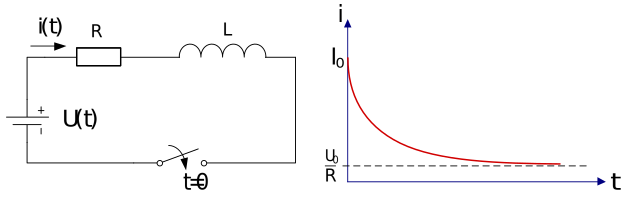
\includegraphics[width=\linewidth]{mai_fig032.pdf}
      \caption{Graf průběhu proudu $i(t)$ po sepnutí spínače v době $t=0$.}
      \label{mai:fig032}
    \end{figure}
%--------------------------------------------------------------------------------------------------- 
%  % !TeX spellcheck = cs_CZ
%---------------------------------------------------------------------------------------------------
% mai2ch05.tex
%---------------------------------------------------------------------------------------------------
\chapter{Řady funkcí}\label{mai:IIchapV}
\minitoc

%---------------------------------------------------------------------------------------------------
\printbibliography[title={Seznam literatury}, heading=subbibliography]
\addcontentsline{toc}{section}{Seznam literatury}
%  % !TeX spellcheck = cs_CZ
%---------------------------------------------------------------------------------------------------
% mai2ch06.tex
%---------------------------------------------------------------------------------------------------
\setchaptertoc
\chapter{Závislosti na více parametrech aneb funkce více proměnných}\label{mai:IIchapVI}
  Skalárními funkcemi jedné reálné proměnné jsme se zabývali velmi podrobně v \ref{part:MAI} dílu.
  Umíme počítat jejich limity v bodech \emph{vlastních} i \emph{nevlastních}, umíme je derivovat i
  integrovat. Totéž dokážeme provádět i s vektorovými funkcemi jedné proměnné. Každý vektor je totiž
  dán svými složkami, takže každá vektorová funkce je zadána tolika „obyčejnými“ skalárními
  funkcemi, kolik má daný vektor složek. S vektoroVými funkcemi jedné proměnné jsme pracovali při
  zadávání trajektorií hmotných bodů a výpočtech jejich dalších charakteristik (rychlost, zrychlení,
  křivost trajektorie, apod). Tou jedinou proměnnou byl obvykle čas. Veličiny popisující objekty a
  děje v přírodě, ať již jsou tyto veličiny skaláry či vektory, však většinou závisí na více
  proměnných než jedné. Kromě času bývají typicky závislé na poloze. Vezměme třeba takové gravitační
  pole Země. Na čase sice nezávisí, zato však klesá s druhou mocninou vzdálenosti od středu Země.
  Veličina, která je charakterizuje, je buď vektorová, nebo skalární. Tou vektorovou je
  \emph{gravitační zrychlení} neboli \emph{intenzita} gravitačního pole Země, tou skalární je
  \emph{potenciál},
  \begin{equation*}
    \vec{g}(\vec{r}) = - \kappa\dfrac{M_Z}{r^2}\left(\dfrac{\vec{r}}{r}\right),\,
    V(\vec{r}) = -\kappa\dfrac{M_Z}{r}, \, r\geq R_Z
  \end{equation*}
  V předchozích Vztazích jsou \(M_Z\) a \(R_Z\) hmotnost a poloměr Země, \(\vec{r}\) je polohový
  vektor místa, v němž pole zjištujeme, vzhledem ke středu Země. Skalární i vektorové veličiny
  popisující elektrické a magnetické pole nábojů a proudů, rychlosti elementů proudící kapaliny nebo
  plynu a řada dalších fyzikálních veličin jsou nejen funkcemi času, ale také polohy bodu, v němž je
  počítáme nebo měříme. A stejně jako byly změny funkcí jedné proměnné vyjádřeny pomocí derivací,
  změny změn pomocí druhých derivací, atd., je třeba umět počítat i změny veličin závisejících na
  více proměnných. Mohou samozřejmě nastat situace, kdy se mění jen jedna z proměnných, zatímco
  ostatní zůstávají konstantní. Nejsnáze si takovou situaci představíme například tak, že měříme
  třeba elektrické pole stále ve stejném bodě prostoru, ale běží při tom čas. Pole se v daném bodě s
  časem mění. Nebo naopak v daném okamžiku sledujeme rozdílnost pole v bodech velmi blízkých danému
  bodu. Obecně se samozřejmě mění všechny proměnné a s nimi i hodnoty skalární funkce nebo složky
  vektorové funkce. Jak takové obecné změny co nejvýstižněji popsat, uvidíme právě v této kapitole.
  Setkáme se v ní s \emph{parciální derivací}, která vystihuje, jak rychle se mění hodnota funkce se
  změnou jedné z proměnných. Dále poznáme obecnější, \emph{směrovou derivaci}, která popisuje
  rychlost změny funkční hodnoty, mění-li se všechny proměnné, ale tak, že bod, který reprezentuje
  soubor jejich hodnot, se pohybuje v prostoru proměnných po libovolné přímce (nikoli jen po jedné
  souřadnicové ose, jako tomu je u parciálních derivací). A konečně zavedeme pojmy \emph{úplného
  diferenciálu} a \emph{Jacobiho zobrazení}, které popisují změnu hodnot skalární či vektorové
  funkce v lineární aproximaci, mění-li se hodnoty proměnných zcela obecně.

  Stejně jako u funkcí jedné proměnné je základem pro definici veličin popisujících rychlost změny
  funkce pojem \textbf{limity}, který úzce souvisí s pojmem \emph{okolí bodů} a obecně i s
  definičními obory funkcí. Pro případ funkcí více proměnných klade požadavek hlubšího pochopení
  pojmu limity větší nároky na soustředěnost a důkladné promýšlení různých situací, než tomu bylo u
  limit funkcí jedné proměnné. Proto se jím zabývá podstatná část poměrně rozsáhlého odstavce
  \ref{mai:IIchapVIsecII} poté, co je v odstavci \ref{mai:IIchapVIsecI} věnována značná pozornost
  různým typům definičních oborů funkcí. Čtenář, který se chce rychle propracovat k praktickým
  výpočtům a spokojí se vatím s intuitivním pochopením pojmu limity funkce více proměnných
  (založeným na dobré znalosti definice a vlastností limit funkcí jedné proměnné), může k nim v
  podstatě rovnou přejít s vědomím, že sice bude umět prakticky provádět různé standardní operace s
  funkcemi více proměnných, ale nebude si pravděpodobně vědět rady s netypickými případy. K
  důkladnému pročtení odstavců \ref{mai:IIchapVIsecI} a \ref{mai:IIchapVIsecII} se může samozřejmě
  vrátit kdykoli.

  \section{Podmonožiny euklidovských prostorů \(\mathcal{R}^n\)}\label{mai:IIchapVIsecI}
    S definičními obory funkcí jedné proměnné to bylo docela jednoduché. Byly to Většinou intervaly
    - otevřené intervaly nebo jejich sjednocení, uzavřené intervaly, popřípadě intervaly uzavřené
    jen z jedné strany. Také zde figurovala okolí bodů, ať již ryzí, z nichž byl daný bod vyloučen,
    nebo taková, která daný bod obsahovala. Nic složitého tam nebylo. Aby bylo možné funkce
    derivovat, což byla nejčastější operace, kterou jsme prováděli s cílem zjistit, jak rychle se
    funkce mění, nemohly být definiční obory „moc divoké“. Vždy bylo třeba předpokládat, že bod, v
    němž jsme funkci nebo její změnu vyšetřovali, má okolí, ve kterém je funkce přinejmenším
    definována. Pro případ funkcí více proměnných je to podobné, ale bude třeba se definičním oborům
    věnovat trochu podrobněji. Dejme tomu, že nějaká fyzikální, nebo i nefyzikální veličina bude
    záviset na \(n\) proměnných. Každá z nich může nabývat nějakých hodnot. Funkční hodnota naší
    funkce bude tak jednoznačně určena souborem \(n\) hodnot jednotlivých proměnných. Tuto
    \(n\)-tici budeme považovat za bod v prostoru \(mathcal{R}^n\). S \(n\)-ticemi jsme již
    pracovali v algebře, takže takový popis známe. V algebře jsme však s nimi prováděli algebraické
    operace, sčítání a násobení číslem. Měli jsme tedy v \(mathcal{R}^n\) zavedenou
    \textbf{algebraickou strukturu}. Pro práci s funkcemi a pro sledování jejich změn \uv{bod od bodu}
    potřebujeme v \(mathcal{R}^n\) ještě jinou strukturu. Ta je tvořena okolími, podobně jako tomu
    bylo u funkcí jedné proměnné. Taková struktura se nazývá \emph{topologická} a matematická
    disciplína, která se zabývá topologickými strukturami, se jmenuje \textbf{topologie}.

    Topologickými strukturami se nebudeme zabývat v celé obecnosti, i když je to velmi zajímavé.
    Budeme pracovat pouze se speciálním typem, takzvanou euklidovskou topologtí v \(mathcal{R}^n\).

    \subsection{Okolí bodů, otevřené a uzavřené množiny}
    S pojmem okolí bodu jsme se setkali hned v první části druhé kapitoly prvního dílu. Vzpomínáte?
    Šlo tehdy o okolí bodu \(a\) na reálné ose \(mathcal{R}\). Okolím jsme rozuměli otevřený
    interval \((a - \delta_1,a + \delta_2)\), \(\delta_1, \delta_2 > O\), ryzím okolím pak množinu
    \((a - \delta_1, a + \delta_2)\backslash{a}\), tj. sjednocení otevřených intervalů \((a -
    \delta_1, a) \cup (a, a + \delta_2)\). Sjednocení jakýchkoli otevřených intervalů jsme později
    nazývali otevřenou množinou, doplňky otevřených množin v \(mathcal{R}\) byly uzavřené množiny.
    Vybudovali jsme tak na \(mathcal{R}\) \emph{euklidovskou topologii} (dodatek F prvního dílu).
    Podobná bude situace i ve vícerozměrném případě, tedy v \(mathcal{R}^n\).

  \section{Skalární funkce více proměnných}\label{mai:IIchapVIsecII}
    V předchozím odstavci jsme si vcelku důkladně připravili pojmy týkající se vhodných definičních
    oborů funkcí více proměnných. Nyní budeme tyto funkce definovat a studovat jejich vlastnosti.
    Obdobně jako u funkcí jedné proměnné půjde o limity, spojitost a derivace. Výhoda důkladné
    přípravy pojmů v předchozím odstavci se ukáže již při budování pojmu limity, zejména v
    nevlastním bodě. Samotnému pojmu limity a s ním úzce spjatého pojmu spojitosti bude věnována
    velká pozornost. Někdo se nad tím může pozastavit: Vždyť jak často se s potřebou výpočtu limit
    setkáváme v praktických příkladech? Málo. Potřebujeme spíše derivovat, integrovat, řešit
    diferenciální rovnice. S příklady na limity se setkáváme ponejvíce v matematických sbírkách, kde
    slouží k procvičení naučené látky. Taková úvaha by byla poněkud krátkozraká. Řada vlastností
    funkcí, a vůbec možnost s nimi rozumně operovat při běžných výpočtech, je založena na
    spojitosti. A spojitost je těsně spjata s pojmem limity. Opět by mohla vzniknout námitka, že
    spojitost přece intuitivně dobře chápeme - spojitá funkce nemá „zpřetrhaný“ graf. Umíme si však
    představit graf funkce tří proměnných? Není to dost dobře možné ani u funkce dvou proměnných,
    je-li složitější, nebo chová-li se v okolí některého bodu „podezřelé“. Limitě tedy potřebujeme
    porozumět, i když její výpočet v praktických příkladech skutečně nebude na „denním pořádku“.
    Abychom porozumění podpořili, budeme se vedle teoretických úvah věnovat i řadě praktických
    příkladů.




%---------------------------------------------------------------------------------------------------
%  % !TeX spellcheck = cs_CZ
%---------------------------------------------------------------------------------------------------
% mai2ch07.tex
%---------------------------------------------------------------------------------------------------
\setchaptertoc
\chapter{Základy variačního počtu pro mechaniku}\label{mai:IIchapVII}


%---------------------------------------------------------------------------------------------------

}{
% Debug mode OFF
%======= Kapitola: Vícerozměrná algebra aneb lineární algebra podruhé =============================
  % !TeX spellcheck = cs_CZ
%---------------------------------------------------------------------------------------------------
% mai2ch01.tex
%---------------------------------------------------------------------------------------------------
\setchaptertoc
\chapter{Vícerozměrná linearita aneb lineární algebra podruhé}\label{mai:IIchapI}
  V kapitole \ref{mai:IchapII} dílu \ref{part:MAI} jsme se seznámili s elegantní dámou lineární
  algebrou. Pomocí jejích pravidel jsme nejen řešili soustavy lineárních rovnic, ale také počítali s
  maticemi a vektory. Zatímco operace s maticemi, a koneckonců i řešení lineárních rovnic pomocí
  matic bychom mohli chápat jako užitečnou ekvilibristiku s číselnými soubory, za počítáním s
  vektory se zdálo být přece jen něco hlubšího a závažnějšího. Vázané vektory pro nás totiž byly
  orientovanými úsečkami v trojrozměrném euklidovském prostoru, v němž bylo definováno měření délek
  a úhlů. Volné vektory pak byly množinami stejně velkých a souhlasně rovnoběžných orientovaných
  úseček. Jednalo se tedy o \emph{geometrické objekty}. Každý vektor byl určen svou velikostí a
  směrem. Směr byl přitom zadán například pomocí úhlů mezi daným vektorem a vybranými směry, které
  byly předem pevně zvoleny. Mohli jsme s vektory provádět základní algebraické operace, jimiž jsou
  sčítání vektorů a násobení vektoru číslem, podle pravidel zavedených pro (v tomto případě řádkové)
  matice. S vektory v trojrozměrném prostoru jsme mohli velmi pohodlně počítat jako s trojicemi
  čísel. Na druhé straně jsme vektory vyjadřovali jako lineární kombinace jiných vektorů, tvořících
  v prostoru všech vektorů \emph{bázi}. Koeficienty lineární kombinace, která představovala zápis
  daného vektoru ve zvolené bázi, byly jeho \emph{složkami} v této bázi. Při změně báze se změnily
  složky vektoru, vektor sám však nikoliv. Vektor je stále sám sebou, jen se v různých bázích jinak
  tváří - projeví se jinou trojicí čísel. Protože se však při změně báze změní složky vektoru přesně
  definovaným způsobem (vzpomeňte na transformační vztahy), dokážeme jej vždy rozpoznat. Tuto
  vlastnost, \emph{invarianci vůči volbě báze}, mají všechny geometrické objekty. A je to právě
  algebra, která nám umožňuje tyto objekty reprezentovat číselnými soubory a také tak s nimi
  počítat. Jde-li navíc o objekty řídící se lineárními pravidly. jakými jsou například distributivní
  zákony, je počítání s nimi, v rámci \emph{lineární algebry}, zvláště jednoduché. Oceníme to
  zejména v prostorech vyšší dimenze, než je náš běžný euklidovský prostor. Při počítání s vektory v
  trojrozměrném prostoru, kde umíme měřit délky a úhly a kde platí trigonometrická pravidla, bychom
  se bez rutinních algebraických procedur ještě třeba obešli. Už ale například ve čtyřrozměrném
  časoprostoru, v němž se odehrávají všechny přírodní jevy a v němž je třeba formulovat fyzikální
  zákony, však pro měření délek a úhlů platí jiná pravidla, než jsou obvyklá v běžném, tj.
  trojrozměrném euklidovském, prostoru. Například tam neplatí čtyřrozměrná verze Pythagorovy věty. A
  někdy je příroda dokonce tak nepřívětivá, že nás nutí pracovat i s prostory vícerozměrnými.
  Například jedna z velmi účinných teorií pro výklad chování elementárních částic, teorie strum, je
  založena na geometrii prostoru jedenáctirozměrného. A v takových dimenzích jsme už s jakkoli
  vynikající geometrickou představivostí v koncích. Tehdy se vděčně obracíme k metodám algebry. V
  této kapitole, jak její název napovídá, půjde o algebru lineární
  
  \section{Prostory s vektory}\label{mai:IIchapIsecI}
    V kapitole \ref{mai:IchapII} jsme pracovali s číselnými maticemi typu \(m/n\), tj. soubory 
    čísel uspořádaných v \(m\) řádcích a \(n\) sloupcích, a zavedli jsme pro ně operaci součtu a 
    násobení číslem. Zjistili jsme, že pro sčítání matic a násobení matice číslem platí určitá 
    pravidla. (Jejich souhrn je uveden v samém závěru odstavce \ref{mai:IchapIIsecIIIsubIII}. V 
    odstavci \ref{mai:IchapIIsecIV} jsme zase počítali s vektory. Ty měly jednou \emph{konkrétní 
    podobu} řádkových matic s pravidly pro jejich sčítání a násobení číslem, podruhé, v 
    trojrozměrném prostoru, naopak \emph{konkrétní podobu} orientovaných úseček, resp. množin, 
    které byly orientovanými úsečkami vytvořeny, generovány. Zavedli jsme tenkrát konkrétní způsob 
    sčítání vektorů a násobení vektoru číslem pomocí geometrických operací. Součet dvou vektorů 
    \(\vec{u}\) a \(\vec{v}\) znamenal, že jsme podle zcela určitého pravidla, pravidla 
    vektorového rovnoběžníka přiřadili uspořádané dvojici \([\vec{u},\vec{v}]\) třetí vektor 
    \(\vec{u} + \vec{v}\), násobek vektoru a čísla byl opět vektor \(\alpha\vec{u}\), který jsme 
    přiřadili dvojici \([\alpha,\vec{u}]\) tvořené číslem a vektorem. Uvedli jsem, že pravidla pro 
    tyto \emph{geometrické} operace jsou shodná s pravidly pro počítání s maticemi a lze je dokázat 
    i geometrickými postupy. Množinu volných vektorů generovaných orientovanými úsečkami spolu s 
    uvedenými dvěma operacemi jsme nazvali \textbf{vektorovým prostorem}. Šlo tedy o zcela odlišné 
    množiny základních objektů a zcela odlišným způsobem definované operace, pro které se však dala 
    dokázat tatáž pravidla. Nyní se podíváme na problém definice vektorového prostoru obecněji a 
    poněkud \uv{opačně}. Budeme pracovat s \emph{nosnou množinou} \(V\), a přitom nebude podstatné, 
    jak konkrétně vypadají její prvky. Ani je nebudeme označovat šipkami (u šipek ze zvyku 
    zůstaneme pouze v případě orientovaných úseček v \(\mathbb{R}^1\), \(\mathbb{R}^2\) a 
    \(\mathbb{R}^3\), nebo vektorů s fyzikálním významem). Dále přibereme do hry množinu všech 
    komplexních čísel \(\mathbb{C}\), popřípadě jen množinu všech reálných čísel \(\mathbb{R}\) a 
    definujeme dvě operace (\emph{zobrazení}):
    \begin{subequations}\label{mai:eq046}
      \begin{align}
        V \times V \ni [a,b]            &\longrightarrow c\in V, \label{mai:eq046a}  \\
        \mathbb{C}\times V\ni[\alpha,a] &\longrightarrow d\in V. \label{mai:eq046b}
      \end{align}
    \end{subequations}
    Prvek \(c\) nazýváme \emph{součet} prvků \(a\) a \(b\) a značíme jej \(c = a + b\) prvek \(d\) 
    je \(\alpha\)-\emph{násobek} prvku \(a\) a značíme \(d = \alpha a\). Zobrazení uvedená ve 
    vztazích (\ref{mai:eq046}) však nebudou moci být úplně libovolná. Budeme požadovat, aby měla 
    určité vlastnosti, konkrétně ty, které jsou uvedeny pro matice na konci odstavce 
    \ref{mai:IchapIIsecIIIsubIII}. Teprve pak řekneme, že množina \(V\) spolu s operacemi 
    (\ref{mai:eq046}) splňujícími potřebné požadavky je vektorovým prostorem. Vidíme, že takto naše 
    uvažování výrazně posuneme na abstraktní úroveň. Bude lhostejné, co jsou prvky nosné množiny, 
    bude nepodstatné, jak konkrétně jsou definovány operace sčítání prvků a násobení prvku číslem. 
    Důležité bude jen to, aby abstraktní operace s abstraktními prvky splňovaly konkrétní pravidla. 
    Než však k definici vektorového prostoru přistoupíme, všimneme si ještě některých jiných 
    struktur s jednou nebo dvěma operacemi, které samy do oblasti lineární algebry nepatří, ale 
    mohou být užitečné pro definici vektorového prostoru, popřípadě mají významné fyzikální 
    aplikace.
      
      \subsection{Algebraické struktury s jednou operací, hlavně grupy}
        Při zavádění operací s vektory jsme zcela automaticky využívali toho, že umíme počítat s 
        reálnými, popřípadě i s komplexními čísly. Skutečnost, že čísla umíme sčítat, násobit a 
        provádět s nimi řadu dalších operací, považujeme za tak přirozenou a samozřejmou, že nad ní 
        vůbec nepřemýšlíme. Již samotné operace sčítání a násobení vytvářejí na množině čísel velmi 
        bohatou \textbf{algebraickou strukturu}. Tento pojem si nyní přiblížíme. 
        
        Algebraickou strukturu s jednou operací získáme, vezmeme-li v úvahu první ze zobrazení 
        (\ref{mai:eq046}), nosnou množinu označíme tentokrát podle zvyku \(G\):
        \begin{subequations}\label{mai:eq047}
          \begin{align}
            G \times G \ni [a,b] &\longrightarrow a + b \in G,                  \label{mai:eq047a}\\
            G \times G \ni [a,b] &\longrightarrow a \cdot b \in G.              \label{mai:eq047b}
          \end{align}
        \end{subequations}
        Pokud použijeme první možnosti označení této operace, hovoříme o operaci \emph{sčítání} a 
        \emph{aditivní} struktuře, v případě druhé možnosti o operaci \emph{násobení} a 
        \emph{multiplikativní} struktuře. Toto terminologické rozlišení nemá obecně žádný hlubší 
        význam. Je spíše otázkou zvyklosti a souvisí především s algebraickou strukturou číselných 
        množin, kterou běžně používáme, aniž o ní přemýšlíme (čísla sčítá a násobí školák, 
        obchodník i účetní a o nějaké abstraktní struktuře nic netuší).
        
        Zobrazení (\ref{mai:eq047}) samo o sobě, aniž na ně klademe další požadavky (podstatné je 
        pouze to, že dvěma prvkům nosné množiny přiřadí prvek \emph{téže množiny}), definuje 
        nejjednodušší algebraickou strukturu s jednou operací, zvanou \textbf{grupoid}. Grupoid 
        není pro fyzikální aplikace příliš užitečný, ale je základem pro konstrukci zajímavějších a 
        užitečnějších struktur. Přidáme-li k definici grupoidu požadavek \emph{asociativity} 
        zobrazení \(G \times G \ni [a, b] \longrightarrow a + b \in G\) (nebo \(G \times G \ni [a, 
        b] \longrightarrow a \cdot b \in G\))
        \begin{subequations}\label{mai:eq048}
          \begin{align}
            (a+b) + c          &= a + (b + c),                                  \label{mai:eq048a}\\
            (a\cdot b) \cdot c &= a \cdot (b \cdot c)                           \label{mai:eq048b} 
          \end{align}
        \end{subequations}
        pro libovolné prvky \(a, b, c \in G\), stane se množina \(G\) spolu s operací „\(+\)“, nebo 
        „-“ \textbf{pologrupou}. I pologrupa je z hlediska fyzikálních aplikací poněkud chudá, 
        další požadavek na zobrazení (\ref{mai:eq047}) z ní však již učiní strukturu v matematice i 
        fyzice nepostradatelnou, grupu. Pologrupa, ve které existuje prvek \(0_G\in G\) a současně 
        ke každému prvku \(a \in G\) existuje prvek \((-a) \in G\) tak, že platí
        \begin{subequations}\label{mai:eq049}
          \begin{align}
            a + 0_G  &= 0_G + a = a,                                            \label{mai:eq049a}\\ 
            a + (-a) &= (-a) + a = 0_G,                                         \label{mai:eq049b}
          \end{align}
        \end{subequations}
        se nazývá \textbf{aditivní grupou}. Prvek \(0_G\) je univerzální pro celou grupu (žádný 
        jiný s touto vlastností v grupě \(G\) není) a nazývá se \emph{neutrální prvek grupy} neboli 
        \textbf{nula}, prvek \((-a)\) je \textbf{opačný} k prvku \(a\). Pro dané \(a\) je určen 
        jednoznačně. V případě operace násobení mají vlastnosti \ref{mai:eq049} tvar
        \begin{subequations}\label{mai:eq050}
          \begin{align}
            a \cdot e_G    &= e_G    \cdot a = a,                       \label{mai:eq050a}\\
            a \cdot a^{-1} &= a^{-1} \cdot a = e_G,                     \label{mai:eq050b}
          \end{align}
        \end{subequations}
        a \(G\) se nazývá \textbf{multiplikativní grupou}. Prvek \(e_G\) je opět univerzální pro 
        celou grupu a nazývá se \textbf{neutrální} prvek grupy, neboli \emph{jednička}, prvek 
        \(a^{-1}\) je \textbf{inverzní} k prvku \(a\).
        
        Každá operace \ref{mai:eq047} v množině \(G\), která splňuje vztahy asociativity 
        \ref{mai:eq048} a vztahy specifikující nulu a opačný prvek, nebo jedničku a inverzní prvek 
        typu \ref{mai:eq049}, nebo \ref{mai:eq050}, představuje \emph{grupovou operaci} bez ohledu 
        na to, podobá-li se spíše sčítání, nebo spíše násobení, či dokonce něčemu jinému, například 
        skládání zobrazení. Má-li grupa konečný počet prvků, nazývá se tento počet jejím 
        \emph{řádem}.

        %---------------------------------------------------------------
        % !TeX spellcheck = cs_CZ
\wikitextrule
\begin{example}\label{mai:exam046}
  \textbf{Kolik nul má (aditivní) grupa?}\newline\small
  Jak dokážeme, že má grupa právě jednu nulu? Co když předchozímu tvrzení nebudeme věřit? Můžeme se 
  o jeho pravdivosti přesvědčit? Ten, kdo mu nevěří, si může třeba představit, že grupa má nuly 
  dvě. Označme je \(0_G\) a \(\overline{0}_G\). Vztah \ref{mai:eq049} platí pro libovolný prvek 
  grupy, proto \(0_G + \overline{0}_G = 0_G\) (to jsme brali \(a = 0_G\) a \(\overline{0}_G\) 
  považovali za nulu) a současně \(0_G + \overline{0}_G = \overline{0}_G\) (nyní zase byl prvek 
  \(0_G\) v roli nuly a \(a = \overline{0}_G\)). Je vidět, že \(0_G = \overline{0}_G\). Nula je 
  tedy skutečně jen jedna. Podobnou úvahu můžeme provést pro jedničku multiplikativní grupy. Platí 
  tedy tvrzení:
  
  Neutrální prvek grupy je určen jednoznačně.
  
  Stejně tak bychom mohli mít pochybnosti o tom, že opačný prvek k danému \(a\in G\) je jen jeden. 
  Předpokládejme, že \(b\) a \(c\) jsou dva opačné prvky k \(a\). Platí \(a + b = 0_G\). Přičteme k 
  této rovnosti \(c\) zleva, tj. \(c + a + b = c\). Protože však \(c + a = 0_G\), dostáváme \(b=c\) 
  a tedy:
  
  Opačný (resp. inverzní) prvek k libovolně zvolenému prvku grupy je určen jednoznačně. 
  \normalsize
\end{example}
        %---------------------------------------------------------------
        
        V úvodu odstavce jsme se zmínili o tom, že množiny reálných a komplexních čísel získají 
        zavedením běžných operací sčítání a násobení jistou algebraickou strukturu. Všimněme si 
        jich nyní podrobněji. 
        
        %---------------------------------------------------------------
        % !TeX spellcheck = cs_CZ
\wikitextrule
\begin{example}\label{mai:exam047}
  \textbf{Algebraická struktura a kupecké počty}\newline\small
    Uvažujme o množině reálných čísel \(G = \mathbb{R}\) tak jako bychom je uměli jen 
    sčítat. Násobení si zatím nevšímejme. Sčítání reálných čísel je zobrazení typu prvního 
    vztahu v \ref{mai:eq047}, které bezpochyby splňuje požadavky \ref{mai:eq048} a 
    \ref{mai:eq049}. Neutrálním prvkem \(0_\mathbb{R}\) je \uv{obyčejná} nula, opačným prvkem k 
    číslu \(a\) je \(-a\), položené na reálné ose symetricky k \(a\) vzhledem k nule. Množina 
    reálných čísel s operací sčítání je tedy aditivní grupou. Pro operaci sčítání dokonce platí 
    něco navíc - komutativní zákon
    \begin{equation}\label{mai:eq051}
      a + b = b + a \qquad\text{pro libovolné} a,b\in\mathbb{R}.
    \end{equation} 
    Grupu s komutativním zákonem nazýváme grupou \emph{komutativní} nebo také \textbf{abelovskou}.
    
    Množina reálných čísel s operací sčítání je komutativní grupou.
    
    Nyní se místo na sčítání zaměřme na násobení reálných čísel a znovu posuďme vlastnosti grupy. 
    Násobení reálných čísel je zobrazením typu druhého vztahu v \ref{mai:eq047} a splňuje požadavek 
    asociativnosti \ref{mai:eq048}. Dále je zřejmé, že číslo \(e_\mathbb{R}\) (\uv{obyčejná} 
    jednička) vyhovuje prvnímu požadavku ve vztazích \ref{mai:eq050}. Potíž je s požadavkem druhým. 
    Inverzní prvek najdeme jen k nenulovým číslům. Nula inverzní prvek nemá. Tato zdánlivá drobnost 
    je příčinou toho, že \textbf{množina reálných čísel s operací násobení není grupou}.
  \normalsize
\end{example}
        %---------------------------------------------------------------
        
        %---------------------------------------------------------------
        % !TeX spellcheck = cs_CZ
\begin{mdframed}[style=mdexam]
  \begin{example}\label{mai:exam048}
    \textbf{Algebraická struktura na množině komplexních čísel}\newline
      Množina \(\cmplxset\) komplexních čísel je kartézským součinem reálných os, \(\cmplxset = 
      \mathbb{R} \times \mathbb{R}\), tedy množinou uspořádaných dvojic \([a, b]\) čísel reálných. 
      Značíme \(z = [a, b]\). Reálné číslo \(a = \operatorname{Re}(z)\) je \emph{reálnou} částí 
      komplexního čísla \(z\) a reálné číslo \(b = \operatorname{Im}(z)\) částí \emph{imaginární}. 
      Operace sčítání a násobení komplexních čísel jsou definovány takto:
      \begin{align*}
        \cmplxset\times\cmplxset      &\ni\left[[a_1, b_1],[a_2, b_2]\right] \longrightarrow   \\
          [a_1, b_1] + [a_2, b_2]     &= [a_1 + a_2, b_1 + b_2]\in\cmplxset,                   \\
        \cmplxset\times\cmplxset      &\ni\left[[a_1, b_1],[a_2, b_2]\right] \longrightarrow   \\
          [a_1, b_1] \cdot [a_2, b_2] &= 
          \begin{array}{c}
            \left[a_1 \cdot a_2 - b_1 \cdot b_2\right], \\
            \left[a_1 \cdot b_2 + a_2 \cdot b_1\right]
          \end{array}
          \in\cmplxset.
      \end{align*}
      
      \begin{mdframed}[style=highlight]
        Množina komplexních čísel s operací součtu je komutativní grupou.
      \end{mdframed}
      
      Jejím neutrálním prvkem je číslo \(0_{\cmplxset} = [0,0]\), opačným prvkem k číslu \(z = [a, 
      b]\) je \(-z = [-a, - b]\). Při operaci násobení je neutrálním prvkem číslo [1,0], prvkem 
      inverzním k číslu \(z = [a, b] \neq 0_{\cmplxset}\) je
      \begin{equation*}
        z^{-1} = \left[\dfrac{a}{a^2 + b^2}, \dfrac{-b}{a^2 + b^2}\right].
      \end{equation*}
      
      K číslu \(0_{\cmplxset} = [0,0]\) však inverzní prvek opět neexistuje. Množina komplexních 
      čísel \textbf{není grupou vzhledem k násobení}.
  \end{example}
\end{mdframed}
        %---------------------------------------------------------------
        
        O podmnožině \(H \subset C\) grupy \(G\) s operací sčítání nebo násobení zúženou na \(H\), 
        která je sama grupou, hovoříme jako o \textbf{podgrupě} grupy \(G\). Například množina 
        reálných čísel zapsaných ve tvaru \(z = [a, 0]\) se sčítáním je podgrupou množiny 
        komplexních čísel. Koho grupy nebaví a chce se rychle prokousat k vektorovým prostorům, 
        které jsou koneckonců hlavní náplní našeho příběhu o lineární algebře, může zbytek tohoto 
        odstavce přeskočit. Ale byla by to škoda, grupy jsou opravdu zajímavé.

        %---------------------------------------------------------------
        % !TeX spellcheck = cs_CZ
\begin{mdframed}[style=mdexam]
  \begin{example}\label{mai:exam049}
    \textbf{Struktura aditivní grupy na podmnožinách reálné osy}\newline
      Některé významné podmnožiny reálné osy mají svá zavedená označení. \(\naturalset\) je množina 
      přirozených čísel. \(\intset\) množina celých čísel a \(\ratioset\) množina racionálních 
      čísel. Můžeme se zajímat o to, zda při zúžení definičního oboru operace sčítání na 
      \(\naturalset \times \naturalset\), \(\intset \times \intset\), popřípadě \(\ratioset \times 
      \ratioset\), budou tyto množiny stále ještě grupami. Ihned vidíme, že množina přirozených 
      čísel grupou nebude, neboť neobsahuje nulu ani záporná čísla, která jsou v grupě \(\realset\). 
      opačnými prvky k číslům kladným. Tímto nedostatkem netrpí množiny celých a racionálních čísel, 
      které tedy budou grupami.
  \end{example}
\end{mdframed}
        %---------------------------------------------------------------
        
        %---------------------------------------------------------------
        % !TeX spellcheck = cs_CZ
\wikitextrule
\begin{example}\label{mai:exam050}
  \textbf{Grupy některých číselných objektů}\newline\small

  \normalsize
\end{example}
        %---------------------------------------------------------------

        %---------------------------------------------------------------
        % !TeX spellcheck = cs_CZ
\wikitextrule
\begin{example}\label{mai:exam051}
  \textbf{Grupy nemusí být tvořeny jen čísly}\newline\small
  Operace sčítání nebo násobení si umíme velmi dobře představit, provádíme-li je standardním 
  způsobem s čísly. Definice algebraických struktur jsou však obecné a zahrnují i jiné možnosti. 
  Představme si například krychli, se kterou provádíme \emph{operace symetrie}. Jsou to všechna 
  taková přemístění krychle z počáteční do koncové polohy, která \uv{se nepoznají}. Znamená to, že 
  krychle vypadá v koncové poloze stejně jako ve výchozí. Pokud bychom při přemísťování zavřeli 
  oči, nepoznali bychom že někdo mezitím s krychlí hýbal. Přemístění jsou několikerých typů a 
  definují \textbf{prvky symetrie} krychle. Abychom si je mohli názorně ukázat na obrázcích, 
  označíme vrcholy, popřípadě jiné důležité body krychle písmeny. V některých ukázkách také 
  použijeme hrací kostku. Prvky symetrie krychle můžeme roztřídit do následujících typů:
  \begin{itemize}
    \item \textbf{zrcadlení vzhledem k rovině symetrie} - existuje rovina, jejíž body 
          zůstávají při přemístění v klidu,
    \item \textbf{rotace kolem osy symetrie} - existuje přímka (osa), jejíž body zůstávají 
          při přemístění v klidu,
    \item \textbf{středová inverze} - existuje právě jeden bod (střed inverze), který při 
          přemístění zůstává v klidu,
    \item \textbf{identita} - přemístění do téže polohy, v klidu jsou všechny body krychle
  \end{itemize}
  Jednotlivé typy prvků symetrie jsou znázorněny na obrázcích 4.1 až 4.15. Na prvním z obrázků 4.1 
  jsou vyznačeny tři symetrie krychle, \(\sigma_1\), \(\sigma_2\) a \(\sigma_3\). Zkuste najít a 
  nakreslit další. Druhý z obrázku 4.1. znázorňuje situaci při zrcadlení vzhledem k rovině 
  \(\sigma_2\). Pro klasickou herní kostku pak operaci zrcadlení ilustruje obrázek 4.2.
  
  {\centering
    \captionsetup{type=figure}
    \includegraphics[width=0.4\linewidth]{mai_fig037.png}
    \captionof{figure}{Prvky symetrie krychle - zrcadlení \cite[s.~6]{Musilova2012MA2}
    \label{mai:fig000}}
    \par}
    
    Kolik existuje os symetrie krychle? Zkuste procvičit svou prostorovou představivost a zamyslet 
    se nad touto  otázkou sami ještě dříve, než se podíváte na obrázky. Vezměte si k tomu třeba 
    libovolnou hrací kostku. (Pozor, rozmístění teček na vaší kostce může být jiné, než na té naší, 
    podle které jsou nakresleny obrázky.) Na obrázku 4.3 jsou vyznačeny tři osy symetrie \(o_1^4\), 
    \(o_2^4\), \(o_3^4\).Prvkem symetrie je otočení kolem kterékoli z nich o jedenkrát, dvakrát 
    nebo třikrát \SI{90}{\deg} při čtvrtém otočeni o \SI{90}{\deg} přejde krychle do původní 
    polohy. Osy se proto nazývají čtyřčetné (vyznačeno horním indexem). Obrázek 4.4 znázorňuje 
    konkrétní situaci při otočení o úhel \SI{270}{\deg} kolem osy o, zatímco obrázek 4.5 ukazuje 
    toto otočení pro klasickou herní kostku.
    
    Další čtyři osy symetrie odpovídají tělesovým úhlopříčkám krychle a jsou znázorněny na obrázku 
    4.6. Jsou označeny symboly \(o_1^3\), \(o_2^3\), \(o_3^3\) a \(o_4^3\) a nazývají se trojčetné 
    (víte proč?).
    
    Obrázky 4.7 a 4.8 odpovídají konkrétnímu otočení kolem osy \(o_3^3\) o úhel \SI{270}{\deg}.
    
    Dalších šest os symetrie najdeme v obrázku 4.9. Každá z nich vždy prochází bodem S (průsečíkem 
    tělesových úhlopříček) a spojuje středy protilehlých hran. Tyto dvojčetné osy jsou označeny 
    symboly \(o_1^2\), \(o_2^2\), \(o_3^2\), \(o_4^2\), \(o_5^2\), \(o_6^2\). Konkrétní příklad 
    otočení kolem osy \(o_1^2\) o úhel \SI{180}{\deg} ilustrují obrázky 4.10 a 4.11. Obrázky 4.12 a 
    4.13 znázorňují středovou inverzi a obrázky 4.14 a 4.15 identitu.
    
    Přemístění můžeme \textbf{skládat}, tzn. postupně provádět . Polohy, ve kterých (neoznačená) 
    krychle vypadá stejné, nazveme ekvivalentní. Označme \(A\) určitou polohu krychle a 
    \(\mathcal{P}_A\) množinu všech přemístění krychle mezi kteroukoli dvojici poloh ekvivalentních 
    poloze \(A\). Operaci skládání přemístění definujeme takto: Nechť \(\varrho\ni\mathcal{P}_A\) 
    je přemístění krychle z polohy \(B\) do polohy \(C\) a \(\psi\ni\mathcal{P}_A\) její přemístění 
    z polohy \(C\) do polohy \(D\). Označme jako \(\psi\circ\varrho\) přemístění,
  \normalsize
\end{example}
        %---------------------------------------------------------------
        
      \subsection{Algebraické struktury se dvěma operacemi, hlavně pole}
      
      \subsection{Co je to vektorový prostor?}
        Vektorový  prostor, ve kterém existuje báze s konečným počtem prvků, jsme nazvali
        konečněrozměrným. Nyní víme, že všechny báze konečněrozměrného vektorového prostoru mají
        shodný počet prvků. Jestliže báze daného vektorového prostoru mají \(n\) prvků, nazýváme
        tento prostor \(n\)-\emph{rozměrným}. Říkáme také, že jeho \emph{dimenze} je \(n\) a značíme
        jej \(V_n\), aby dimenze, jeho důležitá charakteristika, byla přímo součástí označení.
        
        Ukážeme si nyní konkrétní příklady konečněrozměrných vektorových prostorů a určíme jejich
        dimenzi. Zvolíme příklady, s nimiž jsme se již setkali v odstavcích
        \ref{mai:IchapIIsecIII} a \ref{mai:IchapIIsecIV}, tentokrát však budeme sledovat jejich
        společné rysy odpovídající axiomům abstraktního vektorového prostoru. 
        %---------------------------------------------------------------
        % !TeX spellcheck = cs_CZ
\begin{mdframed}[style=mdexam]
  \begin{example}\label{mai:exam107}
    \textbf{Uspořádané \(n\)-tice komplexních čísel jako vektory}\newline
    Na množině uspořádaných \(n\)-tic komplexních čísel
    \begin{equation*}
      a=(\alpha^1,\alpha^2,\ldots,\alpha^n)\in\cmplxset\times\cmplxset\times\cdots\times\cmplxset
    \end{equation*}
    zavedeme operace sčítání
    \begin{align}
      a + b &= (\alpha^1,\alpha^2,\ldots,\alpha^n) + (\beta^1,\beta^2,\ldots,\beta^n)   \nonumber\\
            &= (\alpha^1+ \beta^1,\alpha^2 +\beta^2,\ldots,\alpha^n + \beta^n)    \label{mai:eq098}
    \end{align}
    a násobení skalárem (komplexním číslem)
    \begin{equation}\label{mai:eq099}
      \gamma a = \gamma(\alpha^1,\alpha^2,\ldots,\alpha^n) 
               = (\gamma\alpha^1,\gamma\alpha^2,\ldots,\gamma\alpha^n). 
    \end{equation}
    O tom, že takto konkrétně definované operace splňují všechny axiomy vektorového prostoru nad
    polem komplexních čísel, se snadno přesvědčíme sami. Jde nyní o to, zda se jedná o prostor
    konečné dimenze a jaká tato dimenze je. Označme
    \begingroup
    \setlength{\arraycolsep}{0pt}
    \begin{equation*}
    \begin{array}{rl}
      % https://tex.stackexchange.com/questions/114959/putting-row-of-dots-in-an-equation
      e_1     &= (1, 0, 0, \ldots, 0, 0),  \\
      e_2     &= (0, 1, 0, \ldots, 0, 0),  \\
      \hdotsfor{2}                         \\
      e_{n-1} &= (0, 0, 0, \ldots, 1, 0),  \\
      e_n     &= (0, 0, 0, \ldots, 0, 1).
    \end{array}
    \end{equation*}
    \endgroup
  \end{example}
\end{mdframed}
        %---------------------------------------------------------------

  \section{Lineární zobrazení vektorových prostorů}\label{mai:IIchapIsecII}
  \section{Vektorové prostory se skalárním součinem}
    \subsection{Ortogonální doplňky}
      Nechť \(U\) je podprostor vektorového prostoru \(V\). Ortogonální doplněk $U^\bot$ obsahuje 
      všechny vektory, které jsou kolmé ke každému vektoru z \(U\), neboli \(\forall\vec{v}\in 
      U^\bot\quad \forall\vec{u}\in U\quad \vec{u}\bot\vec{v}\) což lze vyjádřit pomocí skalárního 
      součinu \(\vec{u}\cdot\vec{v} = 0\)

      Ortogonální doplněk \(U^\bot\) k podprostoru \(U = \langle\vec{u}_1,\ldots,\vec{u}_k\rangle\) 
      tedy hledáme jako řešení homogenní soustavy rovnic
      \begin{equation*}
        \left(
          \begin{array}{c|c}
            \vec{u}_1  &   0      \\
            \cdots     &  \vdots  \\
            \vec{u}_k  &   0
          \end{array}
        \right),
      \end{equation*}
      nuly na pravé straně při výpočtu zpravidla vynecháváme. Připomeňme také vztah
      \begin{equation}\label{LA:eq_dim_doplnek}
        \dim U + \dim U^\bot = \dim V
      \end{equation}

      %---------------------------------------------------------------
        % !TeX spellcheck = cs_CZ
% Musilova2009MA1

\begin{example}\label{mai:exam011}
  Zjistěte ortogonální doplněk \(\langle(1,-3,2),(2,1,5)\rangle\bot^.\). (Zdroj:
  \cite[s.~3]{MosnaMA3})
  \newline\textbf{Řešení}:
  Hledáme vektor \((x, y, z)\), jehož skalární součin je se zadanými vektory roven nule. Budeme 
  tedy řešit (úpravou na Gaussův tvar pomocí elementárních úprav) homogenní soustavu rovnic
  zadanou maticí
  \begin{equation*}
     \left(
       \begin{array}{ccc|c}
          1  &  -3  & 2 & 0 \\
          2  &   1  & 5 & 0
       \end{array}
     \right)\sim
     \left(
       \begin{array}{ccc|c}
          1  &  -3  & 2 & 0 \\
          0  &   7  & 1 & 0
       \end{array}
     \right)\
  \end{equation*}
  Odtud dostáváme \(z = \alpha\), \(7y + z = 0\) \(\Rightarrow\) \(y = -\frac{1}{7}\alpha\), \(x
  +\frac{3}{7}\alpha + 2\alpha = 0\) \(\Rightarrow\) \(x = -\frac{17}{7}\) neboli 
  \begin{equation*}
  (x, y, z) =\alpha\left(-\frac{17}{7}, -\frac{1}{7}, 1\right) = \alpha(17, 1, -7)
  \end{equation*}

  V dalších příkladech budeme nuly na pravé straně soustavy vynechávat a upravovat na
  výhodnější tvar
  \begin{equation*}
       \begin{pmatrix}
          1  &  -3  & 2  \\
          2  &   1  & 5
       \end{pmatrix}
       \sim
       \begin{pmatrix}
          1  &  -3  & 2 \\
          0  &   7  & 1
       \end{pmatrix}
       \sim
       \begin{pmatrix}
          1  &   0  & \frac{17}{7}  \\
          0  &   7  & 1
       \end{pmatrix}
       \sim
       \begin{pmatrix}
          7  &   0  & 17 \\
          0  &   7  & 1
       \end{pmatrix}.
  \end{equation*}
  Odtud již snadno zjistíme, že vektor \((x, 1, -7)\) jistě vyhovuje druhé rovnici. Dosadíme-li ho 
  do první rovnice, dostaneme \(7x + 17\cdot(-7) = 0\) a \(x = 17\).

  Hledaný ortogonální doplněk je tedy lineární obal $$\langle(17, 1, -7)\rangle^\bot.$$
  
    {\centering
     \captionsetup{type=figure}
    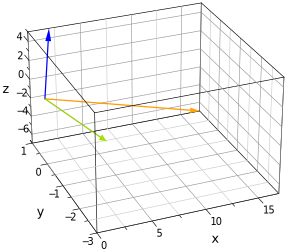
\includegraphics[width=0.5\linewidth]{mai_fig025.pdf}
    \captionof{figure}[Ortogonální doplněk]{Vizualizace vektorového prostoru a jeho    
             ortogonálního doplňku pomocí sw MatLab - MuPAD příkazem:\newline
             \texttt{plot(plot::Arrow3d([1,-3,2]), plot::Arrow3d([2,1,5]), 
             plot::Arrow3d([17,1,-7]))}}
    \label{LA:fig_ort01}
    \par}
\end{example}

      %---------------------------------------------------------------

      Výsledek předchozího příkladu \ref{mai:exam011} lze interpretovat tak, že jsme našli všechny 
      vektory, které jsou kolmé na rovinu určenou vektory ze zadání. Rovina je útvar       
      dvojrozměrný a protože prostor všech vektorů je trojrozměrný, musí nutně mít podprostor 
      ortogonálních vektorů ve shodě se vztahem \ref{LA:eq_dim_doplnek} pouze jednu dimenzi. Vše 
      je dobře patrné z obr. \ref{LA:fig_ort01}

  %=========================== Kapitola: Vlastní čísla a vlastní vektory ==========================
  \section{Vlastní čísla a vlastní vektory}\label{mai:IIchapIsecIII}
    \subsection{Motivace} 
      \textbf{Poznámka}: Je-li \(\mathcal{A} : \mathcal{V} \rightarrow \mathcal{V}\) lineární 
      zobrazení z prostoru \(\mathcal{V}\) do prostoru \(\mathcal{V}\) (nikdy se takové zobrazení 
      nazývá lineárním operátorem), pak je přirozeným požadavkem najít takovou bázi prostoru 
      \(\mathcal{V}\), že je matice zobrazení $\mathbf{A}$ v této bázi co nejjednodušší, např. má 
      následující strukturu
      \begin{equation*}
         \mathbf{A}=
           \left(\begin{array}{ccccc}
             \boxed{A_1}       &             &       &       & 0   \\
                 & \boxed{A_2} &             &       &             \\
                 &             & \boxed{A_3} &       &             \\
                 &             &             &\ddots &             \\
              0  &             &             &       & \boxed{A_k}
            \end{array}
           \right),
     \end{equation*}
     kde \(A_k\) jsou čtvercové matice malého řádu (nejlépe \(1\) nebo \(2\)) a ostatní prvky 
     matice jsou nulové. Problém najít bázi, aby v ní matice zobrazení měla diagonální tvar (kde 
     \(A_k\) jsou skaláry), vede k pojmu vlastní číslo a vlastní vektor matice.

      \begin{definition} 
        Nechť \(\mathbf{A}\in \mathcal{C}^{n,n}\) (matice je čtvercová řádu \(n\)).
        \begin{equation}
          \mathbf{A} = (a_{ij}) =
            \begin{pmatrix}
              a_{11} & a_{12} & \ldots & a_{1n} \\
              a_{21} & a_{22} & \ldots & a_{2n} \\
              \vdots & \vdots & \ddots & \vdots \\
              a_{n1} & a_{n2} & \ldots & a_{nn}
            \end{pmatrix}
        \end{equation}

        Jestliže platí
        \begin{equation}\label{eq:vl_number}
          \mathbf{Au} = \lambda\mathbf{u}
        \end{equation}
        pro jisté komplexní číslo \(\lambda\in\mathcal{C}\)  a jistý nenulový vektor 
        \(x\in\mathcal{C}^n, \mathbf{u}\neq\Theta\), potom číslo \(\lambda\) nazýváme 
        \textbf{vlastním číslem} matice \(\mathbf{A}\) a vektor \(\mathbf{u}\) \textbf{vlastním 
        vektorem} příslušným k tomuto vlastnímu číslu. Množinu všech vlastních čísel nazýváme 
        \textbf{spektrem matice} \(\mathbf{A}\). Pokud rov. \ref{eq:vl_number} rozepíšeme, dostaneme
        \begin{equation}
          \begin{pmatrix}
            a_{11} & a_{12} & \ldots & a_{1n} \\
            a_{21} & a_{22} & \ldots & a_{2n} \\
            \vdots & \vdots & \ddots & \vdots \\
            a_{n1} & a_{n2} & \ldots & a_{nn}
          \end{pmatrix}   \cdot
          \begin{pmatrix}
            u_{1} \\  u_{2} \\ \vdots \\  u_{n} \\
          \end{pmatrix}    =\lambda\cdot
          \begin{pmatrix}
            u_{1} \\ u_{2} \\ \vdots \\ u_{n} \\
          \end{pmatrix}
        \end{equation}
        můžeme ji rovněž psát ve tvaru
        \begin{equation*}
            \begin{pmatrix}
            \setlength{\arraycolsep}{3pt}
              a_{11} -\lambda & a_{12}           & \ldots & a_{1n} \\
              a_{21}          & a_{22} -\lambda  & \ldots & a_{2n} \\
              \vdots          & \vdots           & \ddots & \vdots \\
              a_{n1}          & a_{n2}           & \ldots & a_{nn}-\lambda
            \end{pmatrix} \cdot
          \begin{pmatrix}
            u_{1} \\ u_{2} \\ \vdots \\ u_{n} \\
          \end{pmatrix}  =
          \begin{pmatrix}
              0 \\ 0 \\ \vdots \\ 0 \\
            \end{pmatrix}
        \end{equation*}
      \end{definition}

       Tato soustava rov. je \textbf{homogenní} a stručně ji můžeme zapsat
      \begin{equation}\label{vv_hom_zapis}
        \left(\mathbf{A} - \lambda\mathbf{I}\right) = \mathbf{0}
      \end{equation}
      Homogenní soustava má \emph{netriviální řešení}, právě když je determinant matice soustavy 
      roven  nule, tj. v případě soustavy rov. rov. \ref{vv_hom_zapis} platí
      \begin{equation}\label{vv_hom_reseni}
        \abs{\mathbf{A} - \lambda\mathbf{I}} = \mathbf{0}
      \end{equation}
      Determinant \(A(\lambda)=\abs{\mathbf{A} - \lambda \mathbf{I}}\) nazýváme 
      \textbf{charakteristický polynom} matice \(\mathbf{A}\) - jedná se o polynom stupně \(n\) v 
      proměnné \(\lambda\), který má v oboru komplexních čísel \(n\) kořenů. Rovnici 
      \(A(\lambda)=0\) nazýváme \textbf{charakteristická rovnice matice \(\mathbf{A}\)} - jejími 
      kořeny jsou \textbf{charakteristické hodnoty} (resp. \textbf{vlastní čísla}) 
      \textbf{matice} \(\mathbf{A}\).
            
      \begin{tcnote}
        U vlastních čísel studium pouze reálných matic ztrácí smysl, protože i 
        reálná matice může mít komplexní vlastní čísla. Proto se uvažuje obecná komplexní matice.
      \end{tcnote}
      
      \begin{tcnote}
        Podmínka existence nenulového vektoru \(\mathbf{u} = \Theta\) v definici 
        vlastního čísla je nezbytná: kdyby bylo připuštěno i \(\mathbf{u} = \emptyset\), potom by 
        každé komplexní číslo bylo vlastním číslem a definice by ztratila smysl.
      \end{tcnote}
      
      \begin{tcnote}
        Odpovídá-li matice \(\mathbf{A}\) matici nějakého zobrazení \(\mathcal{A}\), pak každý 
        nenulový vektor z jádra zobrazení \(\ker\mathcal{A}\) je vlastním vektorem příslušným 
        vlastnímu číslu \(\lambda\). Je-li \(\ker\mathcal{A} = \{\Theta\}\) 
        (je-li matice \(\mathbf{A}\) regulární), pak \(\Theta\) není vlastním číslem matice 
        \(\mathbf{A}\).
      \end{tcnote}

      %---------------------------------------------------------------
        % !TeX spellcheck = cs_CZ
\begin{mathexam}{Ortogonální projekce v prostoru \(\mathcal{R}^3\)}{exam012}
    Je-li \(\mathbf{P}\) matice ortogonální projekce v prostoru \(\mathcal{R}^3\) na nějaký 
    podprostor \(\mathcal{U}\) (\(\mathcal{U}\) je tedy buď rovina nebo přímka procházející 
    počátkem), pak pro každý vektor \(\mathbf{u}\in\mathcal{U}\) platí \(\mathbf{Pu} = 
    \mathbf{u}\), všechny vektory z \(\mathcal{U}\) (s výjimkou nulového vektoru \(\Theta\)) 
    jsou vlastními vektory matice $\mathbf{P}$ příslušné vlastnímu číslu \(\lambda\). Prostor 
    \(\mathrm{U}^\bot\) je roven jádru projekce (nulovému prostoru matice \(\mathbf{P}\)), 
    a tedy každý vektor z ortogonálního doplňku \(\mathcal{U}\) (s výjimkou \(\Theta\)) je 
    vlastním vektorem příslušným k vlastnímu číslu \(0\).

    {\centering
      \captionsetup{type=figure}
      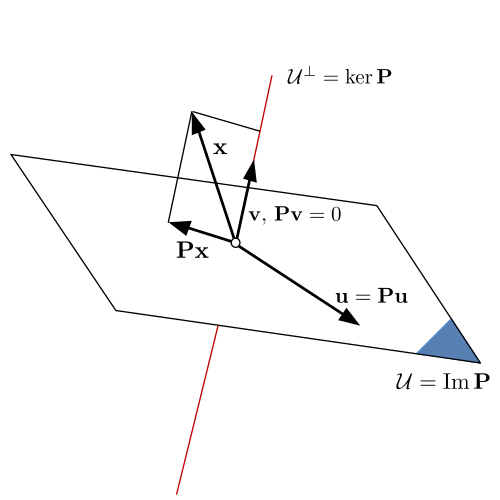
\includegraphics[width=0.5\linewidth]{mai_fig024.pdf}
      \captionof{figure}{K příkladu \ref{mai:exam012}}
      \label{MAI:FIG016}
      \par}

\end{mathexam}
      %---------------------------------------------------------------

      %---------------------------------------------------------------
        % !TeX spellcheck = cs_CZ


\begin{example}\label{mai:exam013}
  Určete spektrum matice a její spektrální poloměr následující matice
    \begin{equation*}\label{pr:spektrum_matice}
      \mathbf{A} =
        \begin{pmatrix}
          2  &  2    & 0 \\
         -3  & -3    & 5 \\
          0  & -0.25 & 2
        \end{pmatrix}
    \end{equation*}
  \textbf{Řešení}: Spektrum matice je množina všech jejích vlastních čísel. Spektrální poloměr 
  je maximum z absolutních hodnot vlastních čísel. Vlastní čísla určíme z charakteristické
  rovnice \(\det(\mathbf{A}-\lambda \mathbf{I})=0\).
    \begin{equation*}
      \textbf{A} - \lambda\textbf{I}=
        \begin{pmatrix}
          2-\lambda  &  2          & 0 \\
         -3          & -3-\lambda  & 5 \\
          0          & -0.25       & 2-\lambda
       \end{pmatrix}
    \end{equation*}
    \begin{align}
      \det(\mathbf{A}-\lambda \mathbf{I})                    &= 0           \nonumber\\
      (2-\lambda)
        \begin{pmatrix}
          -3-\lambda  &  5\\
             -0.25    &  2 - \lambda
        \end{pmatrix} -2\cdot
        \begin{pmatrix}
          -3       &  5\\
           0       &  2 - \lambda
        \end{pmatrix}                                        &= 0           \nonumber\\
      (2-\lambda)^2(-3-\lambda)+1.25(2-\lambda)+6(2-\lambda) &= 0           \nonumber\\
      (2-\lambda)[(2-\lambda)(-3-\lambda)+1.25+6]            &= 0           \nonumber\\
      (2-\lambda)(\lambda^2+\lambda+1.25)                    &= 0           \nonumber
    \end{align}
    \begin{equation*}
      \lambda_1 = 2, \quad\lambda_2 = -0.5+i, \quad\lambda_3=-0.5-i
    \end{equation*}
    \begin{itemize}
      \item Spektrum matice \(\mathbf{A}\) je \(\sigma(\mathbf{A})=\{2,-0.5+i,-0.5-i\}\).
      \item Spektrální poloměr \(\rho(\mathbf{A})=\max_i|\lambda_i|=2\).
    \end{itemize}

%    \attachfile[icon=Paperclip, description=Matlab Determine the spectrum of a matrix 
%      and its spectral radius]{../SRC/MAI/matlab/LA001.m}

\end{example}
      %---------------------------------------------------------------

      %---------------------------------------------------------------
        % !TeX spellcheck = cs_CZ
\begin{example}\label{mai:exam014}
  Určete vlastní čísla a vlastní vektory matice \(\mathbf{B} = \mathbf{A}^2 - 4\mathbf{A} + 
  9\mathbf{A}^{-1} - \mathbf{I}\), kde \(\mathbf{A}\) je matice \(\mathbf{A}= 
  \begin{pmatrix}1&0.5\\3.5&4\end{pmatrix}\).

  \textbf{Řešení}: (z předchozího příkladu víme, že \(\lambda_1=4.5, \lambda_2=0.5\)) a
   \(\mathbf{I}\) jednotková matice. Označme symbolem \(\lambda\) vlastní číslo matice 
   \(\mathbf{A}\) a nechť \(\mathbf{x}\) je příslušný vlastní vektor. Pak platí:
   \begin{itemize}
     \item Matice \(\mathbf{A}^2\) má vlastní čísla rovna \(\lambda^2\).
     \item Matice \(4\mathbf{A}\) má vlastní čísla rovna \(4\lambda\).
     \item Matice \(9\mathbf{A}^{-1}\) má vlastní čísla rovna \(\frac{9}{\lambda}\).
   \end{itemize}
   Matice \(\mathbf{B}=\mathbf{A}^2-4\mathbf{A}+9\mathbf{A}^{-1}-\mathbf{I}\) má vlastní čísla 
   ve tvaru  \(\lambda^2-4\lambda+\frac{9}{\lambda}-1\), vlastní vektory jsou stejné jako 
   vlastní vektory odpovídající vlastním číslům matice \(\mathbf{A}\). Tedy:
   \begin{equation*}
       \sigma(B)=\{4.5^2-4\cdot4.5+\frac{9}{4.5}-1,\quad
       0.5^2-4\cdot0.5+\frac{9}{0.5}-1\}=\{3.25, 15.25\}
   \end{equation*}
\end{example}
      %---------------------------------------------------------------


      %---------------------------------------------------------------
       % !TeX spellcheck = cs_CZ
\begin{mathexam}{Určete vlastní čísla a odpovídající vlastní vektory následují\-cích matic:
  \begin{equation*}
    \mathbf{A}=
      \begin{pmatrix}
        1   & 0.5\\
        3.5 & 4
      \end{pmatrix}, \quad
    \mathbf{B}=
      \begin{pmatrix}
        3   & -1 \\
        2.5 &  4 
      \end{pmatrix}
  \end{equation*}
  }{exam002}

  Vlastní čísla určíme z charakteristické rovnice: \(\det(\mathbf{A} - \lambda\mathbf{I}) = 0\).
  Vlastní vektory \(\mathbf{x_i}\) odpovídající vlastním číslům \(\lambda_i\), jsou řešením
  homogenní soustavy rovnic \((\mathbf{A} - \lambda_i\mathbf{I})\mathbf{x_i} = 0\).
  \begin{itemize}
    \item Vlastní čísla matice \textbf{A}:
      \begin{equation*}
          \textbf{A} - \lambda\textbf{I} =
            \begin{pmatrix}
                1-\lambda  &  0.5          \\
              -3.5         &  4-\lambda
            \end{pmatrix}
      \end{equation*}
      \begin{align*}
        \det(\mathbf{A}-\lambda\mathbf{I}) &= 0 \\
        (1-\lambda)(4-\lambda)-\frac{7}{4} &= 0 \\
        \lambda^2-5\lambda+\frac{9}{4}     &= 0
      \end{align*}
      \begin{equation*}
        \lambda_1 = 4.5,\quad \lambda_2 = 0.5
      \end{equation*}
  \end{itemize}

  \begin{itemize}
    \item Vlastní čísla matice \textbf{B}:
      \begin{equation*}
          \textbf{B} - \lambda\textbf{I}=
            \begin{pmatrix}
              3-\lambda  & -1             \\
              2.5        &  4-\lambda
            \end{pmatrix}
      \end{equation*}
      \begin{align*}
        \det(\mathbf{B}-\lambda\mathbf{I}) &= 0 \\
        (3-\lambda)(4-\lambda)+\frac{5}{2} &= 0 \\
        \lambda^2-7\lambda+\frac{29}{2}    &= 0
      \end{align*}
      \begin{equation*}
        \lambda_1 = \frac{7+3i}{2},\quad \lambda_2 = \frac{7-3i}{2}
      \end{equation*}
  \end{itemize}
  % matice A
  Vlastní vektor matice \(\mathbf{A}\) pro \(\lambda_1=4.5: (\mathbf{A} -
  \lambda_1\mathbf{I})\mathbf{x_1} = 0 \Rightarrow\)
  \begin{equation*}
    \begin{pmatrix}
      1  -4.5  &  0.5     \\
      -3.5     &  4-4.5
    \end{pmatrix}
    \sim
    \begin{pmatrix}
      -3.5  &  0.5         \\
      -3.5  & -0.5
    \end{pmatrix}
  \end{equation*}
  \begin{equation*}
    \Rightarrow\mathbf{x_1} =
    \begin{pmatrix}
      1 \\ 7
    \end{pmatrix}
    \, r, r\in\mathbb{R}, r\neq0
  \end{equation*}
  Vlastní vektor matice \(\mathbf{A}\) pro \(\lambda_2=0.5: (\mathbf{A} -
  \lambda_1\mathbf{I})\mathbf{x_2}=0 \Rightarrow\)
  \begin{equation*}
    \begin{pmatrix}
      1  -0.5  &  0.5   \\
      -3.5      &  4-0.5
    \end{pmatrix}
    \sim
    \begin{pmatrix}
      0.5  &  0.5       \\
      3.5  &  3.5
    \end{pmatrix}
  \end{equation*}
  \begin{equation*}
    \Rightarrow\mathbf{x_2} =
    \begin{pmatrix}
      -1 \\ 1
    \end{pmatrix}
    \, r, r\in\mathbb{R}, r\neq0
  \end{equation*}
  % matice B
  Vlastní vektor matice \(\mathbf{A}\) pro \(\lambda_1=\frac{7+3i}{2}: (\mathbf{B} -
  \lambda_1\mathbf{I})\mathbf{x_1}=0 \Rightarrow\)
  \begin{align*}
    \begin{pmatrix}
      3 - \frac{7+3i}{2}            & -1                                       \\
      \frac{5}{2}                   &  4 - \frac{7+3i}{2}
    \end{pmatrix}
    &\sim
    \begin{pmatrix}
      -\frac{1}{2}-\frac{3}{2}i      &  -1                                     \\
      \frac{5}{2}                    & \frac{1}{2}-\frac{3}{2}i
    \end{pmatrix}
    \sim                                                                            \\
    \begin{pmatrix}
      -\frac{10}{4}                  &-\left(\frac{1}{2} -\frac{3}{2}i\right)  \\
      \frac{5}{2}                    & \frac{1}{2}-\frac{3}{2}i
    \end{pmatrix}
    &\sim
    \begin{pmatrix}
      -5                           &-\left(1-3i\right)                         \\
        5                           & \left(1-3i\right)
    \end{pmatrix}
  \end{align*} 
  \begin{align*} 
    \Rightarrow \mathbf{x_1}=
    \begin{pmatrix}
      -1+3i \\ 5
    \end{pmatrix}
    \, r, r\in\mathbb{C}, r\neq0
  \end{align*}
  Vlastní vektor matice \(\mathbf{B}\) pro \(\lambda_2=\frac{7-3i}{2}: (\mathbf{B} -
  \lambda_1\mathbf{I})\mathbf{x_2}=0 \Rightarrow\)
  \begin{align*}
    \begin{pmatrix}
      3  - \frac{7-3i}{2}       &  -1                                     \\
      \frac{5}{2}               &  4 - \frac{7-3i}{2}
    \end{pmatrix}
    &\sim
    \begin{pmatrix}
      -\frac{1}{2}+\frac{3}{2}i  &  -1                                     \\
      \frac{5}{2}                & \frac{1}{2}+\frac{3}{2}i
    \end{pmatrix}                                 
    \sim                                                                          \\
    \begin{pmatrix}
      -\frac{10}{4}              &-\left(\frac{1}{2} +\frac{3}{2}i\right)  \\
      \frac{5}{2}                & \quad\frac{1}{2}+\frac{3}{2}i
    \end{pmatrix}
    &\sim                                                                   
    \begin{pmatrix}
      -5                         &-\left(1+3i\right)                       \\
      5                          & \quad\left(1+3i\right)
    \end{pmatrix}
  \end{align*} 
  \begin{equation*} 
    \Rightarrow \mathbf{x_2}=
    \begin{pmatrix}
      -1-3i \\ 5
    \end{pmatrix}
    \, r, r\in\mathbb{C}, r\neq0
  \end{equation*}
  %---------------------------------------------------------------
  \lstinputlisting[%
    style=luaMatlabStyle,
    caption={Výpis programu pro ověření výpočtu vlastních čísel matic programem Matlab.}
    ]{../src/MAI/matlab/LA001.m}
  %--------------------------------------------------------------- 
\end{mathexam}
      %---------------------------------------------------------------


%---------------------------------------------------------------------------------------------------
%======= Kapitola: Souřadnicové soustavy obvyklejší i méně obvyklé ================================
  % !TeX spellcheck = cs_CZ
%---------------------------------------------------------------------------------------------------
% mai2ch02.tex
%---------------------------------------------------------------------------------------------------
\setchaptertoc
\chapter{Souřadnicové soustavy obvyklejší i méně obvyklé}\label{mai:IIchapII}


%---------------------------------------------------------------------------------------------------
%======= Kapitola: Linearita v aplikacích aneb lineární algebra do třetice ========================
  % !TeX spellcheck = cs_CZ
%---------------------------------------------------------------------------------------------------
% mai2ch03.tex
%---------------------------------------------------------------------------------------------------
\chapter{Linearita v aplikacích aneb lineární algebra do třetice}\label{mai:IIchapIII}
\minitoc

%---------------------------------------------------------------------------------------------------
\printbibliography[title={Seznam literatury}, heading=subbibliography]
\addcontentsline{toc}{section}{Seznam literatury}
%======= Kapitola: Obyčejné diferenciální rovnice =================================================
  % !TeX spellcheck = cs_CZ
%---------------------------------------------------------------------------------------------------
% mai2ch04.tex
%---------------------------------------------------------------------------------------------------
\setchaptertoc
\chapter{Obyčejné diferenciální rovnice}\label{mai:IIchapIV}

  V partii \ref{part:MAI} jsme se seznámili s funkcemi, o jejich užitečnosti nepochybujeme, neboť
  jsme se již přesvědčili, že se s nimi setkáváme takřka na každém kroku. Vyjadřují totiž
  jednoduchým způsobem vzájemnou souvislost veličin, a nejen fyzikálních. Známe-li například funkci
  vyjadřující závislost polohy tělesa na čase, můžeme zjistit, kde těleso v daném okamžiku bylo, je,
  nebo bude. Známe-li funkce, které popisuji časový vývoj cen a platů, můžeme snadno zjistit, zda za
  stejný peníz, za který dnes dostaneme deset housek, koupíme za rok dvacet, nebo jen dvě. Příroda,
  a ani ekonomika či politika, však nejsou natolik průhledné, aby nám takové závislosti předestřely
  přímo. Poskytují pouze informace o jejich změnách, a to ještě ukryté ve speciálních rovnicích,
  zvaných \emph{diferenciální}. Jde-li o neznámou reálnou funkci nebo soubor funkcí závislých na
  jedné reálné proměnné, třeba na čase, hovoříme o obyčejných diferenciálních rovnicích. Přesněji
  řečeno, diferenciální rovnice vyjadřuje matematickou formou zákon platný pro hledanou funkci a
  její derivace prvního nebo i vyšších řádů. Takovou funkcí času může být například i množství látky
  při chemických reakcích, mohutnost populace živočichů, kurz eura, cena akcií na burze, rychlost
  pohybu těles, teplota atd. Ve fyzice a chemii jsou diferenciální rovnice dány fyzikálními či
  chemickými zákony, v ekonomii nebo biologii se objevují v různých modelech, odpovídajících více či
  méně skutečnosti. Uveďme si několik příkladů, na nichž si vysvětlíme základní terminologii, která
  je s problematikou diferenciálních rovnic spojena.
  
  Doplňková literatura pro studium této partie je například: \cite[s.~217]{Musilova2012MA2} a 
  \cite[s.~426]{Brabec1989}. Pro procvičení elementárních metod řešení konkrétních rovnic je vhodná 
  sbírka řešených příkladů \cite[s.~348]{Jirasek1989}.
  
  %--Příklad s hlemýžděm------------------------------------------
      % !TeX spellcheck = cs_CZ
% Musilova2009MA2
\begin{mdframed}[style=mdexam]
  \begin{example}\label{mai:exam084}
    \textbf{Pohyb po přímce}\newline
    Hlemýžď se pohybuje po přímce od kopretiny k pampelišce stálou rychlostí \(v_0 =
    \SI{2}{\mm\per\s}\). V počátečním okamžiku \(t = 0\) byl ve vzdálenosti \(s_0 = \SI{10}{\mm}\)
    od kopretiny. Jaká bude jeho vzdálenost od kopretiny v libovolném okamžiku \(t\geq0\)? Na tuto
    otázku by jistě snadno odpověděl i žák první třídy. Ukažme si však, že úlohu lze také vyjádřit
    pomocí diferenciální rovnice. Vzdálenost \(s(t)\) je hledanou funkcí jedné proměnné, a to času
    \(t\). Rychlost \(v_0\) rovnoměrného přímočarého pohybu je časovou derivací vzdálenosti.
    Získáváme tedy rovnici

    {\centering
     \captionsetup{type=figure}
     \luafigure[0.7]{mai_fig055.png}
     \captionof{figure}{Hlemýžď pohybující se po přímce od kopretiny k pampelišce 
                       \cite[s.~217]{Musilova2012MA2}}
     \label{mai:fig055}
    \par}
    
    \begin{equation}\label{mai:eq076}
      \der{s(t)}{t} = v_0.
    \end{equation}

    Již jsme se zmínili, že rovnice obsahující neznámou reálnou funkci jedné reálné proměnné a její
    derivace obecně i vyššího řádu se nazývá obyčejnou diferenciální rovnicí. Každá z funkcí, které
    rovnici splňují, se nazývá jejím řešením. Řád rovnice je určen nejvyšší derivací, která se v
    rovnici vyskytuje, v našem příkladu jde tedy o rovnici prvního řádu.

    {\centering
     \captionsetup{type=figure}
     \luafigure[1]{mai_fig054.png}
     \captionof{figure}{Graf řešení počáteční úlohy (\ref{mai:eq077}).}
     \label{mai:fig054}
    \par}
    
    Řešení rovnice (\ref{mai:eq076}) snadno \uv{uhodneme}. Bude jím každá funkce
    \begin{equation*}
      s(t) = v_0t +C,
    \end{equation*}
    kde \(C\) je libovolné reálné číslo. Funkce, které jsou řešením rovnice, mají stejný charakter a
    jsou odlišeny pouze číselnou hodnotou \(C\), tvoří soubor, který se nazývá \textbf{obecné řešení
    rovnice}. Ze všech funkcí, které vyhovují rovnici (\ref{mai:eq076}), však skutečný pohyb
    hlemýždě popisuje právě jedna. Abychom ji našli, potřebujeme určit správnou hodnotu \(C\). K
    jejímu zjištění stačí, abychom věděli, jaká byla poloha hlemýždě v jediném okamžiku. Jestliže
    jsme například začali měřit čas ve chvíli, kdy byl hlemýžď ve vzdálenosti \(s_0\) od kopretiny,
    máme tzv. \textbf{počáteční podmínku} \(s(0) = s_0\). Pomocí ní můžeme z nekonečně mnoha funkcí
    obecného řešení vybrat jediné \textbf{partikulární řešení}. V našem případě to bude funkce
    \(s(t) = v_0t + s_0\). Naše rovnice společně s počáteční podmínkou, tj.
    \begin{equation}\label{mai:eq077}
      \der{s(t)}{t} = v_0, \qquad s(0) = s_0,
    \end{equation}
    představuje tzv. \textbf{počáteční úlohu}. Její řešení je v grafu na obrázku \ref{mai:fig054}
    vyznačeno červeně, modře jsou vyznačena některá další partikulární řešení. Dokážete určit, jaké
    počáteční úloze odpovídají?
  \end{example}
\end{mdframed}
  %---------------------------------------------------------------
  Ve většině příkladů, se kterými se setkáme, bude mít počáteční úloha právě jedno řešení, jak tomu
  je v případě hlemýždě. Jestliže je nějaká funkce, definovaná na intervalu \((a,b)\), řešením
  počáteční úlohy, pak každá funkce, kterou vytvoříme zúžením původního řešení na „menší“ interval,
  bude opět rovnici splňovat. My však máme \emph{„právě jedním řešením“} na mysli tzv. \textbf{úplné
  řešení}, tj. takové, které není zúžením žádného jiného, a tak řešení lišící se pouze definičním
  oborem nebudeme považovat za odlišná. Jak uvidíme později, vyskytnou se však také příklady, kdy
  počáteční úloha nemá žádné řešení, nebo jich má naopak nekonečně mnoho.

  %--Příklad s koupelnou------------------------------------------
      % !TeX spellcheck = cs_CZ
% Musilova2009MA2
\begin{mdframed}[style=mdexam]
  \begin{example}\label{mai:exam085}
    \textbf{Příklad s koupelnou}\newline
      V koupelně o celkovém objemu \(V = \num{12000}\) litrů byl nainstalován větrák, jehož výkon je
      \(P = \num{400}\) litrů za minutu. Položme si otázku: Jaká je optimální doba, na kterou je
      třeba nastavit časový spínač, aby větrák neběžel příliš dlouho a přitom se vyměnil všechen
      vzduch v místnosti? A je to vůbec možné? Může se opravdu vzduch vyměnit všechen? Přemýšlejme o
      této situaci důkladněji. Označme \(c(t)\) funkci popisující okamžitou objemovou koncentraci
      „původního vzduchu“ v místnosti, tj. poměr objemu původního vzduchu ku objemu místnosti. (V
      okamžiku zapnutí větráku, tj. pro \(t = 0\), je \(c(0) = c_0 = 1\), v okamžiku, kdy bude
      původní vzduch zcela vyčerpán, pokud to vůbec nastane, bude \(c = 0\).) V intervalu \([t,t +
      \Delta t]\) větrák odčerpá \(P\Delta t\) litrů vzduchu celkem, z toho množství starého vzduchu
      činí \(c(t)P\Delta t\) a jeho podíl na celkovém množství vzduchu je \(c(t)P\Delta t/V\). Tato
      hodnota představuje pro velmi malé \(\Delta t\) \textbf{úbytek} koncentrace starého vzduchu v
      koupelně v časovém intervalu \([t, t + \Delta t]\), tj.
      \begin{equation*}
        \Delta c(t) = - \frac{c(t)P\Delta t}{V} \Rightarrow 
        \dfrac{\Delta c(t)}{\Delta t} = - \dfrac{P}{V}c(t)
      \end{equation*}
      
      (uměli bychom vysvětlit záporné znaménko?). Získáváme rovnici
      \begin{equation}\label{mai:eq078}
        \der{c(t)}{t} = - \dfrac{P}{V}c(t)
      \end{equation}
      Dosazením snadno ověříme, že řešením rovnice (\ref{mai:eq078}) je každá funkce
      \begin{equation*}
        c(t) = Ke^{-\frac{Pt}{V}},
      \end{equation*}

      {\centering
      \captionsetup{type=figure}
      \luafigure[1]{mai_fig056.png}
      \captionof{figure}{Graf řešení úlohy s koupelnou.}
      \label{mai:fig056}
      \par}
      
      kde \(K\) je libovolné číslo. Jeho konkrétní hodnotu pro náš případ určíme z počáteční
      podmínky \(c(0) = 1\), tj. \(K = 1\). A vida, pokud jsme počítali správně, můžeme usoudit, že
      koncentrace původního vzduchu neklesne na nulovou hodnotu nikdy. Naše řešení samozřejmě
      nevylučuje použití časového spínače - rozumně bychom mohli například požadovat, aby
      koncentrace původního vzduchu klesla na hodnotu \(c(\tau) = \num{0.1}\). Hledaná doba bude \(t
      =\frac{P}{V}\ln(1/c(\tau)) =\qty{69}{\minute}\). Řešení naší počáteční úlohy je v grafu na
      obrázku \ref{mai:fig056} vyznačeno červeně. Jakým počátečním úlohám odpovídají modré křivky?
  \end{example}
\end{mdframed}
  %---------------------------------------------------------------
  
  \begin{tcnote}
    „Větrací“ rovnice, diskutovaná v předchozím případě, se ve fyzice objevuje poměrně často. Někdy
    je nazývána lineárním diferenciálním zákonem. Narazíme na ni vždy, když je rychlost změny nějaké
    veličiny (její první derivace) přímo úměrná veličině samotné. Tak například při rozpadu
    radioaktivních jader dospějeme k rovnici \(\der{N(t)}{t} = -\lambda N(t)\), kde \(N(t)\) je
    počet radioaktivních jader ve vzorku v okamžiku \(t\) a \(\lambda\) je \textbf{rozpadová
    konstanta}. Při zkoumání absorpce rentgenového záření v látce získáme rovnici \(\der{I(x)}{x} =
    -\mu I(x)\), kde \(I(x)\) je intenzita v hloubce \(x\) pod povrchem a \(\mu\) je lineární
    \textbf{koeficient absorpce}. S oběma příklady jsme se již setkali v partii \ref{part:MAI}.
    Zkusme si vzpomenout na další příklady lineárních diferenciálních zákonů.
  \end{tcnote}

  %--Příklad o sáňkování------------------------------------------
      % !TeX spellcheck = cs_CZ
% Musilova2009MA2
\begin{mdframed}[style=mdexam]
  \begin{example}\label{mai:exam086}
    \textbf{Příklad o sáňkování}\newline
    Kdo bude rychlejší na sáňkách? Tatínek o hmotnosti \(M\), nebo Pepíček s Mařenkou o hmotnosti
    \(m\)? Každý fyzik hned namítne, že tíhové zrychlení, které určuje rozjezd sáněk, na hmotnosti
    nezávisí. Z praxe však víme, že tatínkové bývají rychlejší. Jak to? Zřejmě proto, že sáňkování
    ve vakuu není obvyklé. Kromě průmětu tíhové síly do nakloněné roviny (\(F_1 = Mg\sin\alpha\)),
    který „nás urychluje", jsme brzděni silou odporu prostředí. V jednoduchém přiblížení ji můžeme
    předpokládat ve tvaru \(F_2 = -Cv^2\). Konstanta \(C\) závisí na tvaru a rozměrech pohybujícího
    se objektu a na hustotě vzduchu. Pro jednoduchost předpokládáme, že je stejná u tatínka i
    Pepíčka. Fyzikální zákon \(Ma= F_1 + F_2 = Mg\sin\alpha - Cv^2\)

    {\centering
    \captionsetup{type=figure}
    \luafigure[1]{mai_fig057.jpg}
    \captionof{figure}{Ladův obrázek dětí na sáňkách.}
    \label{mai:fig057}
    \par}

    například pro tatínka můžeme přepsat na diferenciální rovnici takto:
    \begin{equation}\label{mai:eq079}
      M\der{v}{t} = Mg\sin\alpha - Cv^2
    \end{equation}
    
    Hledanou funkcí je nyní časová závislost rychlosti, jako počáteční podmínku budeme uvažovat, že
    rychlost v čase \(t = 0\) byla nulová. Řešením této počáteční úlohy je funkce
    \begin{align*}
      v(t) &= \sqrt{\dfrac{Mg\sin\alpha}{C}}
              \left[\dfrac{e^{2t\sqrt{\dfrac{Cg\sin\alpha}{M}}}-1}
                          {e^{2t\sqrt{\dfrac{Cg\sin\alpha}{M}}}+1}
              \right]                                                                           \\
          &= \sqrt{\dfrac{Mg\sin\alpha}{C}}\tanh\left(t\sqrt{\dfrac{Cg\sin\alpha}{M}}\right).
    \end{align*}
    Graf takovéto závislosti pro dvě různé hmotnosti \(M = \SI{100}{\kg}\) (červená) a \(m =\SI{10}
    {\kg}\) (modrá) vidíme na obrázku \ref{mai:fig057}. (Poměr hmotností byl takto zvolen pro
    zvýraznění rozdílnosti výsledků - každému je zřejmé, že mimino samo sáňkovat nemůže.) Další
    hodnoty: \(\alpha = \ang{20}\), \(g = \SI{10}{\m\per\square\s}\), \(C =
    \SI{1.00}{N\m^2s^{-2}}\). Na obrázku \ref{mai:fig058} si všimněme, že rychlost se nejprve

    {\centering
    \captionsetup{type=figure}
    \luafigure[1]{mai_fig058.png}
    \captionof{figure}{Graf řešení úlohy o sáňkování. \cite[s.~221]{Musilova2012MA2}}
    \label{mai:fig058}
    \par}

    poměrně prudce zvyšuje, ale poté se asymptoticky blíží k tzv. \textbf{mezní rychlosti} \(v_{max}
    = Mg\sin\alpha\). Mezní rychlost odpovídá situaci, kdy se síly \(F_1\) a \(F_2\) „vyrovnají“.
    (Taková situace však nenastane, je pouze limitním případem pro \(t \rightarrow \infty\).) 
  \end{example}
\end{mdframed}
  %---------------------------------------------------------------
  \begin{tcnote}
    Zamysleme se také nad tím, jak jsme z vyjádření funkce \(v(t)\) pomocí exponenciálních funkcí 
    získali elegantnější výraz s hyperbolickou tangentou. Pro připomenutí hyperbolických funkcí se 
    můžeme vrátit k odstavci 2.1.8 partie \ref{part:MAI}.
  \end{tcnote}
  
  Na uvedených příkladech jsme se mohli přesvědčit, že porozumění některým realistickým dějům
  vyžaduje umět sestavit a řešit diferenciální rovnice. Problémy, se kterými se v životě setkáváme,
  však obvykle vedou k rovnicím mnohem komplikovanějším. Proto často používáme aproximací a skutečný
  svět si poněkud „idealizujeme". Tak například v úloze s koupelnou jsme předpokládali, že vzduch v
  místnosti je vždy dokonale promíchán, v úloze o sáňkování jsme pro odporovou sílu použili pouze
  přibližný zákon a zanedbali třecí sílu. Často se setkáme s rovnicemi, které dokážeme řešit pouze
  numerickými metodami za pomoci počítačů. Aproximativní přístupy tedy mohou vstupovat do popisu
  vývoje reálných systémů pomocí diferenciálních rovnic dvojím způsobem. Poprvé již při samotném
  sestavení diferenciálních rovnic, podruhé při jejich řešení.
  
  V této kapitole se budeme věnovat některým typickým situacím, kdy je možné získat řešení
  diferenciálních rovnic analytickými metodami, zjednodušeně řečeno „tužkou na papíře“. Proč se
  omezujeme na některé typické situace“? Protože problematika diferenciálních rovnic obsahuje ještě
  další úskalí. Řečeno s mírnou nadsázkou, existuje totiž nepřeberné množství různých typů
  diferenciálních rovnic, dokonce už v případě rovnic prvního řádu, které při řešení vyžadují takřka
  \uv{individuální přístup}. I když samozřejmě v teorii diferenciálních rovnic existuje řada
  obecných výsledků společných určité širší skupině diferenciálních rovnic, není možné formulovat
  nějaký \uv{univerzální} postup, který by vedl k řešení kterékoli z nich. V praxi je proto třeba
  naučit se rozpoznat jednotlivé typy obyčejných diferenciálních rovnic a zvolit pro jejich řešení
  vhodnou metodu. Ne nadarmo se proto textům o diferenciálních rovnicích říká „kuchařky“, aniž by to
  mělo hanlivý nádech. (Vznešenější slovo pro „kuchařku“ je „příručka“. Pokud jde o problematiku
  obyčejných diferenciálních rovnic, je takovou moderní příručkou kniha \cite{PolyaninZaitsev},
  která na více než osmi stech stran obsahuje přes 6 200 rovnic s řešeními!
  
  \twocolumn[\section{Diferenicální rovnice vyskytující se kolem nás}\label{mai:IIchapIVsecI}]
    V tomto odstavci jsou zařazeny motivační příklady ukazující, že diferenciální rovnice se
    skutečně objevují v různých vědních oborech. Rovnice jsou většinou uvedeny bez řešení, ale jsou
    doplněny alespoň odkazy ve kterých lze najít mnohem více informací, které jdou za rámec této
    partie o obyčených diferenciálních rovnicích. Stejně jako v předchozích příklad, řada
    fyzikálních principů má tvar výroku, resp. vztahu mezi jistými veličinami (funkcemi) a jejich
    změnami, vztaženými ke zvoleným nezávisle proměnným (pa\-ra\-me\-trům) (\emph{čas, souřadnice}).
    Je to přirozené, neboť (\emph{okamžité}, či \emph{okální}) změny se nejlépe vystihují pomocí
    derivací. Takový zákon má pak charakter vztahu mezi uvažovanými veličinami a jejich derivacemi. 
    
    \begin{tcnote}
      V matematických textech o obyčejných diferenciálních rovnicích se označuje nezávisle proměnná
      obvykle symbolem \(x\), neznámá funkce \(y = y(x)\) nebo \(y = f(x)\) a její derivace čárkami,
      tj. \(y'(x)\), \(y''(x)\) nebo \(y' = f'(x)\), \(y'' = f''(x)\) atd. V mnoha fyzikálních i
      jiných praktických situacích však bývá nezávisle proměnnou čas \(t\) a hledáme závislost
      veličiny \(x = x(t)\) na čase. Tohoto značení budeme velmi často používat, přičemž první,
      resp. druhou derivaci funkce \(x(t)\) budeme podle zvyklosti zavedené ve fyzice vyznačovat
      pomocí tečky, resp. dvou teček nad symbolem \(x\),
      \begin{equation*}
        \dot{x}(t) = \der{x}{t}, \qquad \ddot{x}(t) = \dder{x}{t}.
      \end{equation*}
      Pro větší přehlednost zápisu budeme často vynechávat argument \(t\) v závorce, \(\dot{x} = 
      \dot{x}(t)\). Nebudeli řečeno jinak, předpokládáme, že všechny funkce jsou spojité, případně 
      i diferencovatelné na celém svém definičním oboru nebo alespoň na jistém oboru, který je jeho 
      podmnožinou. Při práci s podílem funkcí budeme automaticky předpokládat, že jmenovatelem je 
      funkce, která je nenulová ve všech bodech uvažovaného intervalu.      
    \end{tcnote}
    
    \subsection{Diferenciální rovnice v mechanice}
      \textbf{Druhý Newtonův pohybový} zákon pro hmotný bod, který nabývá tvaru
      \begin{equation*}
        m\vec{a} = \vec{F}
      \end{equation*}
      skrývá soustavou \emph{tří diferenciálních rovnic druhého řádu}. Složky zrychlení \(\vec{a}(t)
      = (a_x(t), a_y(t), a_z(t)) = (\ddot{x}(t), \ddot{y}(t), \ddot{z}(t))\) jsou totiž druhými
      derivacemi složek polohového vektoru \(\vec{r}(t) = (x(t), y(t), z(t))\) podle času, vektor
      výslednice sil působících na hmotný bod je obecně funkcí jeho polohy a rychlosti, a často také
      explicitní funkcí času. Platí tedy \(\vec{F} = \vec{F}(\vec{r},\vec{v},t)\). Rozepíšeme-li
      druhý Newtonův zákon do složek, dostaneme
      \begin{align*}
        m\ddot{x} & = F_x(x,y,z,\dot{x}, \dot{y}, \dot{z}, t),        \\
        m\ddot{y} & = F_y(x,y,z,\dot{x}, \dot{y}, \dot{z}, t),        \\
        m\ddot{z} & = F_z(x,y,z,\dot{x}, \dot{y}, \dot{z}, t)
      \end{align*}
      Řešením této soustavy je časová závislost \(\vec{r} = (x(t), y(t), z(t))\) polohového vektoru
      hmotného bodu. Je \emph{parametrickým vyjádřenim křivky}, po které se hmotný bod v prostoru
      pohybuje, nazývá se \emph{trajektorií} pohybu.Zadáním počáteční polohy \(\vec{r}_0 = (x(t_0),
      y(t_0), z(t_0))\) a počáteční rychlosti \(v_0 = (\dot{x}(t_0), \dot{y}(t_0), \dot{z}(t_0))\)
      například v okamžiku \(t_0 = 0\) ziskáme \textbf{počáteční úlohu}. (Soustava obsahuje druhé
      derivace neznámých funkci \(x(t)\), \(y(t)\) a \(z(t)\), proto potřebujeme dvě podmínky pro
      každou z nich.) 
      
      Zapišme takový příklad konkrétní soustavy: Na planetu o hmotnosti \(m\) působí Slunce o
      hmotnosti \(M\) silou \(\vec{F}_g\) danou Newtonovým gravitačním zákonem. Tentokrát však jde o
      tzv. „silový zákon", který popisuje gravitační interakci planety a Slunce. Umístíme-li počátek
      soustavy souřadnic do hmotného bodu představujícího Slunce, platí
      \begin{equation*}
        \vec{F}_g = - \dfrac{\kappa mM\vec{r}}{r^3} 
                  = - \dfrac{\kappa mM}{(x^2+y^2+z^2)^{\frac{3}{2}}}(x, y, z)
      \end{equation*}
      kde \(\kappa =  \SI{6.67e-11}{\N\m^2\kg^{-2}}\) je jednou z univerzálních fyzikálních
      konstant, nazývanou gravitační konstanta. Za předpokladu, že zanedbáme pohyb Slunce a
      gravitační působení planet a ostatních těles, má soustava rovnic vyjadřující druhý Newtonův
      zákon pro planetu tvar 
      \begin{subequations}
        \begin{empheq}[box=\widefbox]{align*}
          m\ddot{x} & = - \kappa mM \dfrac{x}{(x^2+y^2+z^2)^{\frac{3}{2}}},        \\
          m\ddot{y} & = - \kappa mM \dfrac{y}{(x^2+y^2+z^2)^{\frac{3}{2}}},        \\
          m\ddot{z} & = - \kappa mM \dfrac{z}{(x^2+y^2+z^2)^{\frac{3}{2}}}
        \end{empheq}
      \end{subequations}

      Nalézt řešení této soustavy znamená „vydolovat" z ní, při daných počátečních podmínkách,
      konkrétní tvar funkcí \(x(t)\), \(y(t)\) a \(z(t)\). Zrovna tato úloha není příliš jednoduchá.
      Postup při jejím řešení, který lze usnadnit použitím fyzikálních \uv{triků}, si ukážeme později. 

    \subsection{Diferenciální rovnice v chemii}
      Uvažujme o chemické reakci, při které se ze dvou látek \(A\) a \(B\) syntetizuje látka \(C\).
      Na jeden gram výsledné látky je zapotřebí \(p\) gramů látky \(A\) a \(1 - p\) gramů látky
      \(B\). Smícháme \(a\) gramů látky \(A\) s \(b\) gramy látky \(B\). Na počátku je hmotnost
      látky \(C\) nulová, její hodnotu v čase \(t\) označíme \(x(t)\). Rychlost chemické reakce, tj.
      změna hmotnosti látky \(C\) s časem, je v rámci nejjednoduššího modelu rovna veličině \((a -
      px) (b - (1 - p)x)\). Vidíme, že při zvětšujícím se množství výsledné látky bude rychlost
      reakce klesat. Ve výsledku se projeví i to, jaké množství výchozích látek smícháme, resp. jak
      se jejich poměr \(\dfrac{a}{b}\) bude lišit od „ideálního" poměru \(\dfrac{p}{1-p}\). Rovnice
      popisující reakci je diferenciální rovnicí prvního řádu pro časovou závislost \(x(t)\)
      hmotnosti látky \(C\)
      \begin{equation*}
        \boxed{\dot{x} = (a - px)(b - (1-p)x)}\, ,
      \end{equation*}
      s počáteční podmínkou \(x(0) = 0\). K této rovnici se ještě hodí poznamenat, že je příkladem
      (i když velmi speciálním) známé \textbf{Riccatiovy rovnice}, která má uplatnění i v
      praktických disciplínách, například v elektrotechnice nebo v oblasti automatického řízení.
      Přestože má nevinně vypadající obecný tvar \(x(t) = h(t) + f(t)x +g(t)x^2\), \(h(t) \neq 0\),
      \(g(t) \neq 0\), je tak trochu „zrádná“. Její řešení se totiž nemusí podařit zapsat pomocí
      elementárních funkcí. 
    
    \subsection{Diferenciální rovnice v biologii}
      Uvažujme o vlkovi a zajíci. Předpokládáme-li, že zajíc má vždycky co žrát (trávy je všude
      dost), bude nárůst počtu zajíců úměrný jejich okamžitému počtu (čím více je zajíců, tím více
      dalších se narodí). Zároveň jsou zajíci požíráni vlky a jejich úbytek je úměrný jak počtu
      vlků, tak počtu jich samých (čím více je zajíců, tím více jich každý věčně hladový vlk chytí a
      sežere, čím více je vlků, tím více zajíců sežerou). Co se vlků týče, ty nikdo nesežere, ale
      budou umírat hladem, jestliže nebude dostatek zajíců. Nárůst počtu vlků je tedy úměrný jak
      počtu vlků, tak počtu zajíců, kdežto úbytek je úměrný pouze počtu vlků. Získáváme soustavu
      dvou diferenciálních rovnic

      \begin{subequations}
        \begin{empheq}[box=\widefbox]{align*}
          \dot{z} &= \alpha z - \beta zv,     \\
          \dot{v} &= \gamma v + \delta zv,
        \end{empheq}
      \end{subequations}

      kde funkce \(z(t)\) resp. \(v(t)\) vyjadřují časovou závislost počtu zajíců, resp. vlků.
      Konstanty \(\alpha\), \(\beta\), \(\gamma\), \(\delta\) lze určit dlouhodobým pozorováním. 
      \begin{tcnote}
        Pokud někoho napadlo, že zajíci i vlci se také rodí i umírají „přirozenou cestou“, má
        pravdu. Tato skutečnost je v našem jednoduchém modelu zahrnuta. Přirozený přírůstek či
        úbytek zajíců i vlků je také úměrný jejich okamžitému počtu, a je tedy respektován
        empirickými hodnotami \(\alpha\), \(\gamma\).
      \end{tcnote}
      
      Tato soustava nelineárních diferenciálních rovnic se nazývá \textbf{Lotkova-Volterrova}. 
      Existence triviálního, tj. identicky nulového řešení, odpovídajícího situaci, kdy žádný zajíc 
      ani vlk neexistují je zřejmá na první pohled. Rovnice má však také netriviální řešení, které 
      si později ukážeme. 
      
      Obdobným příkladem z biologie je situace, kdy diferenciální rovnice popisuje časový průběh
      vývoje jedné populace. Řekněme, že jde o populaci bakterií, jejíž velikost v závislosti na
      čase je dána funkcí \(P(t)\). Při vývoji hrají roli dva nezávislé faktory, jeden způsobuje
      růst populace a druhý souvisí s omezeními danými prostředím. Představme si situaci tak, že bez
      omezujících vlivů prostředí by populace narůstala podle lineárního diferenciálního zákona, tj.
      derivace \(\dot{P}(t)\) hledané funkce \(P(t)\) by byla v každém okamžiku přímo úměrná hodnotě
      \(P(t)\), konstantu úměrnosti \(R\) nazvěme \emph{faktorem růstu}. Okolní prostředí však
      znemožňuje neomezené narůstání funkčních hodnot \(P(t)\). Růst je totiž modifikován tak, že se
      anuluje v okamžiku, kdy je dosaženo \uv{povolené} hodnoty \(P_{max} = K\), tj. když hodnota
      funkce \(P(t)\) dosáhne úrovně \emph{nosné kapacity} \(K\). Odpovídající diferenciální rovnice
      je opět nelineární a zní
      \begin{equation*}
        \boxed{\dot{P} = RP\left(1 - \dfrac{P}{K}\right)}
      \end{equation*}
      Nazýváme ji \textbf{logistickou rovnicí} a rovněž se ji naučíme vyřešit.
      
    \subsection{Diferenciální rovnice v ekonomii}
      V novinách se občas objeví zpráva, že míra inflace klesá. Od obyvatelstva se očekává, že to
      bude interpretovat jako pozitivní jev v naší ekonomice. Je tomu tak skutečně? Označme jako
      \(h(t)\) funkci popisující vhodným způsobem „kupní sílu“ koruny v závislosti na čase (název
      funkce \(h(t)\) jsme dali do uvozovek, neboť skutečná situace je z pohledu ekonomiky
      složitější a nezávisí pouze na inflaci). Její záporně vzatou derivaci \(\mu = -\der{h(t)}{t} =
      -h\) nazýváme mírou inflace. Proč znaménko minus? Pokud je funkce \(h(t)\) klesající, tj.
      kupní síla peněz se snižuje, je její derivace záporná. O míře inflace se však při znehodnocení
      kupní síly hovoří jako o kladné veličině. Jestliže míra inflace podle novinářů klesá, je její
      derivace \(\mu(t)\) záporná. Předpokládejme pro jednoduchost, že velikost této derivace je
      stálá. Druhá derivace neznámé funkce \(h(t)\) je tedy kladná konstantní hodnota, označme ji
      třeba \(A\), \(A > 0\). Dostáváme velmi jednoduchou diferenciální rovnici
      \begin{equation*}
        \ddot{h} = A.
      \end{equation*}
      kterou můžeme okamžitě vyřešit. Vyhovují jí všechny funkce tvaru
      \begin{align*}
        h(t) &= \dfrac{1}{2}At^2 -\mu_1(t) + h_0 \\
             &= \dfrac{A}{2}\left(t-\dfrac{\mu_1}{A}\right)^2+\left(h_0-\dfrac{\mu_1^2}{2A}\right), 
      \end{align*}
      přičemž význam konstant \(h_0\) a \(\mu_1\) je takový, že \(h_0 = h(0) > 0\) představuje
      počáteční kupní sílu peněz, \(\mu_1 = -\dot{h}(0) = \mu(0) > 0\) je počáteční míra inflace.
      Grafem řešení rovnice je parabola, která má konvexní průběh, neboť \(\ddot{h} = A > 0\). Její
      vrchol (minimum) odpovídá bodu \(t_0 = \mu_1/A\). V tomto okamžiku dosáhne míra inflace nulové
      hodnoty. V časovém intervalu \([0, t_0]\) tedy kupní síla našeho platu i přes optimisticky
      vypadající novinovou zprávu stále klesá, tento pokles se však postupně zmírňuje a v okamžiku
      \(t_0\) je nulový - od tohoto okamžiku již neplatí původní tvrzení, že míra inflace klesá
      (nemůže být totiž záporná, nešlo by o inflaci). Interval \([0, t_0]\) je tedy oborem, na
      kterém je řešení diferenciální rovnice pro daný případ relevantní, i když řešení rovnice
      existuje na celé reálné ose.
      
      Jiný ekonomický model může představovat ,spojité" úročení vkladu v bance. Předpokládejme, že
      úrok činí konstantní část \(k\), obvykle několik procent, okamžité výše vkladu. Je-li výše
      vkladu popsána funkcí \(x(t)\), pak
      \begin{equation*}
        \dot{x} = kx.
      \end{equation*}
      Počáteční podmínku můžeme zadat třeba ve tvaru \(x(0) = x_0\). Podobně jako v příkladu s 
      koupelnou je řešením této rovnice exponenciální funkce.
      
    \subsection{Diferenciální rovnice v kuchyni}
      Představme si právě uvařený čaj nebo kávu. Jakými pravidly se řídí jejich vychládání? Jistě
      bude velký rozdíl v tom, zda nalejeme čaj do hrnku, nebo do termosky. Podívejme se, jaká
      diferenciální rovnice bude popisovat jeho chladnutí v obou případech. Označme \(T_0\) teplotu
      okolí. V případě, že čaj bude mít možnost volně si vyměňovat energii s okolím, bude rychlost
      poklesu jeho teploty přímo úměrná rozdílu teploty čaje a okolí (příspěvek způsobený tepelným
      zářením můžeme zanedbat). Získáme tak diferenciální rovnici
      \begin{equation*}
        \dot{T} = c(T_0 - T)
      \end{equation*}
      pro časovou závislost teploty čaje \(T = T(t)\). V případě, kdy bude čaj nalit do dokonale
      izolující nádoby a nemá tak možnost si vyměňovat teplo s okolím, je jeho chladnutí způsobeno
      pouze přenosem energie prostřednictvím elektromagnetického záření. Energie přenášená tepelným
      zářením je úměrná čtvrté mocnině teploty. Chladnutí čaje bude popisovat diferenciální rovnice
      \begin{equation*}
        \dot{T} = k(T_0^4 - T^4)
      \end{equation*}
      Popsané situace jsou však značným zjednodušením skutečných procesů.
    
    \subsection{Diferenciální rovnice v technických aplikacích}
      Pokud přijmeme konstatování, že technika je, velmi zhruba řečeno, v podstatě aplikovaná fyzika
      (technická mechanika, elektrotechnika, apod.), je zřejmé, že o příklady použití
      diferenciálních rovnic nebude nouze. Vezměme například nejjednodušší kmitavý elektrický obvod
      s rezistorem o odporu \(R\), cívkou o indukčnosti \(L\) a kondenzátorem o kapacitě \(C\).
      Kondenzátor v okamžiku \(t = 0\) nabijeme na napětí \(U_0\), a necháme obvod „jeho osudu“. Co
      se bude dít? Kondenzátor se zjevně začne vybíjet, obvodem poteče proud. Jak bude záviset
      okamžité napětí \(u_C(t)\) na kondenzátoru na čase? Jak bude na čase záviset proud \(i(t)\) v
      obvodu? Odpověď na to dá diferenciální rovnice, kterou získáme z podmínky, že součet úbytků
      napětí na kondenzátoru, cívce a odporu musí být v každém okamžiku nulový, tj.
      \begin{equation*}
        u_c(t) + u_L(t) + u_R(t) = 0.
      \end{equation*}      
      Pro jednotlivé úbytky napětí platí
      \begin{gather*}
        u_C(t) = \dfrac{1}{C}\int i(t)\dd{t}, \quad  u_L(t) = \der{i(t)}{t} \quad u_R(t) = Ri(t),
      \end{gather*}
      kde \(Q(t)\) je funkce popisující časovou závislost náboje na kondenzátoru. Odtud pak 
      dostáváme tzv. \emph{integrodiferenciální rovnici} a jejím zderivováním získáme diferenciální 
      rovnici druhého řádu.
      \begin{equation*}
        \dfrac{1}{C}\int i(t)\dd{t} + L\der{i(t)}{t} + Ri(t) = 0 \Rightarrow
        \ddot{i} + \dfrac{R}{L}\dot{i} + \dfrac{1}{LC}i = 0.
      \end{equation*}
      Počáteční úloha je zadána podmínkami \(i(0) = 0\) a \(u_C(0) = U\). (Rovnice platí za 
      předpokladu, že elektromagnetické pole obvodu se mění dostatečně pomalu, je kvazistacionární.)
      
    \subsection{Diferenciální rovnice v přírodě}
      Touto ukázkou jsme možná měli naši pomyslnou „procházku“ použitím diferenciálních rovnic v
      životě začít. Předchozí příklady byly totiž zaměřené vždy speciálně - buď na konkrétní
      aplikaci, nebo trochu obecněji, na zákonitosti typické pro některý z dílčích fyzikálních oborů
      (například mechaniku). Pořadí příkladů jsme takto volili proto, abychom nejprve osvětlili
      jednodušší situace. Diferenciálními rovnicemi se však řídí osudy přírody samy o sobě. Výstižně
      to charakterizoval jeden z významných fyziků, nositel Nobelovy ceny Richard Feynman: „Zákony
      vesmíru mají samy o sobě povahu diferenciálních rovnic.“ Takové diferenciální rovnice, které
      popisují přírodní zákonitosti, budou jistě složitější než naše předchozí ukázky, přinejmenším
      v tom smyslu, že příroda se vyvíjí jednak v čase, jednak v prostoru. Fyzikální veličiny
      popisující takový vývoj budou tedy často záviset na tom, kdy a kde se daný jev odehrává. A to
      už máme čtyři nezávisle proměnné - čas a tři souřadnice polohy dané události. Veličina se mění
      jak s plynutím času, tak se změnou kterékoli souřadnice. Tyto změny popisujeme
      \textbf{parciálními derivacemi}, s nimiž jsme se již stručně seznámili v kapitole
      \ref{mai:IIchapVIII}. 
      
      Při popisu přírodních zákonitostí máme tedy často co do činění s parciálními diferenciálními
      rovnicemi. K nejznámějším z nich patří \emph{Maxwellovy rovnice elektrodynamiky}, které
      popisují časoprostorový vývoj základních veličin elektromagnetického pole
      \(\vec{E}(t,\vec{r})\) (\emph{elektrická intenzita}) a \(\vec{B}(t,\vec{r})\)
      (\emph{magnetická indukce}), nebo \emph{vlnová rovnice}, jejímž řešením jsou všechny vlnové
      děje. Také rovnice pro jeden z nejjednodušších objektů mikrosvěta, atom vodíku, je parciální
      diferenciální rovnicí, stejně jako obecná rovnice pro vývoj stavu kvantověmechanického
      objektu, tzv. \emph{časová Schrödingerova rovnice}. Poslední dva případy, ale i řada dalších,
      však mají své důležité specifikum, pro které má smysl hovořit o nich v kapitole o obyčejných
      diferenciálních rovnicích. Za jistých okolností či zjednodušujících předpokladů, a zejména z
      důvodů symetrie, která ve fyzice hraje důležitou roli, lze hledání jejich řešení převést na
      řešení soustavy rovnic obyčejných.  Je to v situacích, kdy lze závislost hledané funkce více
      proměnných převést na hledání několika funkcí jedné proměnné. Abychom toto obecné konstatování
      alespoň poněkud konkretizovali, všimněme si nejjednoduššího systému podléhajícího zákonům
      kvantové mechaniky, jehož stav je závislý na čase \(t\) a jedné souřadnici, například \(x\).
      Takovým systémem může být například volná částice vázaná na osu \(x\). Aniž bychom zabíhali do
      fyzikálních podrobností (naším úkolem je zabývat se matematickými záležitostmi), řekněme si
      pouze tolik, že stav takového systému lze charakterizovat funkcí \(\Psi(t,x)\), která se řídí
      časovou Schrödingerovou rovnicí
      
      \begin{equation*}
        \imath\hbar\pder{\Psi}{t} = -\dfrac{\hbar^2}{2m}\ppder{\Psi}{x},
      \end{equation*}
      kde \(\hbar = \dfrac{h}{2\pi}\), \(h = \SI{6.63e-34}{\J\cdot\s}\) je \emph{Planckova 
      konstanta}, \(m\) je \emph{hmotnost částice}. Značný význam mají taková řešení této rovnice, 
      která lze zapsat ve tvaru součinu dvou funkcí, z nichž každá závisí pouze na jedné proměnné, 
      tj. \(\Psi(t,x) = \chi(t)\varphi(x)\). Pro 
      takové funkce platí
      
      \begin{align*}
        \pder{\Psi(x,t)}{t}  &= \varphi(x)\der{\chi(t)}{t} = \varphi(x)\dot{\chi}(t), \\
        \ppder{\Psi(x,t)}{t} &= \chi(x)\dder{\varphi(x)}{x} = \chi(t)\varphi''(x)
      \end{align*}
      Dosazením do původní parciální rovnice a její úpravou dostáváme
      \begin{equation*}
        \imath\hbar\dfrac{\dot{\chi}(t)}{\chi(t)} = 
            -\dfrac{\hbar^2}{2m}\dfrac{\varphi''(x)}{\varphi(x)}.
      \end{equation*}
      Je vidět, že pravá strana takto upravené rovnice je jen funkcí souřadnice, zatímco levá závisí
      jen na čase. To však není možné splnit jinak, než že obě strany rovnice jsou rovny téže
      konstantě, řekněme \(E\). Problém nalezení řešení parciální diferenciální rovnice jsme
      převedli na problém nalezení řešení dvou rovnic obyčejných
      \begin{equation*}
        \dfrac{\varphi''(x)}{\varphi(x)} = -\dfrac{2mE}{\hbar^2}, \qquad
        \dfrac{\dot{\chi}(t)}{\chi(t)} = -\imath\dfrac{E}{\hbar}
      \end{equation*}
      Řešení těchto dvou rovnic, stejně jako další příklady převedení parciálních rovnic na
      obyčejné, si ukážeme později. V tuto chvíli však již vidíme, že řešením obyčejných
      diferenciálních rovnic má smysl se zabývat nejen z cvičných důvodů, popřípadě pro účely jejich
      použití ve speciálních aplikacích, ale i z obecnějších fyzikálních pohnutek. 
      \cite[s.~229]{Musilova2012MA2}
    
\section{Terminologie}\label{mai:IIchapIVsecII}
  V závěru odstavce ještě shrneme a doplníme obecnou terminologii týkající se diferenciálních
  rovnic, kterou jsme postupně zaváděli v komentářích k jednotlivým příkladům. 
  
  \begin{mathdef}{Obyčejná diferenciální rovnice \(n\)-tého řádu}{def008}
    Obyčejnou diferenciální rovnicí \(n\)-tého řádu nazýváme rovnici tvaru 
    \begin{equation}\label{mai:eq091}
      F(t, x, \dot{x}, \ddot{x}, \ldots,x^{(n)}) = 0
    \end{equation}
    kde \(F(p_1, p_2, \ldots, p_{n+2})\) je funkce definovaná na jisté otevřené souvislé podmnožině
    \(\mathcal{D}\) \((n+2)\)-rozměrného euklidovského prostoru \(\realset^{n+2}\),
    \(\mathcal{D}\subset \realset^{n+2}\). Každá funkce \(x = x(t)\), která je definována na jistém
    intervalu \(\mathcal{I} \subset\realset\) i se svými derivacemi až do řádu \(n\) včetně, pro
    všechna  splňuje \(t\in\mathcal{I}\) podmínku \((t, x(t), \dot{x}(t), \ddot{x}(t), \ldots
    x^{(n)}) \in\mathbb{D}\) a vyhovuje rovnici (\ref{mai:eq091}), se nazývá \textbf{řešením
    rovnice}. Její graf na intervalu \(\mathcal{I}\) je \textbf{integrální křivka}. Jestliže jsou
    \(x_1(t)\), resp. \(x_2(t)\) dvě řešení rovnice definovaná na intervalech \(\mathcal{I}_1\),
    resp. \(\mathcal{I}_2 \subset \mathcal{I}_1\), která na intervalu \(\mathcal{I}_2\) splývají,
    nazývá se \(x_1(t)\) \textbf{prodloužením řešení} \(x_2(t)\) na interval \(\mathcal{I}_1\), a
    \(x_2(t)\) je \textbf{zúžením} neboli \textbf{restrikcí řešení} \(x_1(t)\) na interval
    \(\mathcal{I}_2\).
  \end{mathdef}
  
  \begin{tcnote}
    Pojem \emph{otevřené souvislé podmnožiny}, tzv. oblasti, jsme sice přesně nezavedli, ale
    intuitivně jej dobře chápeme. Typickým příkladem oblasti v prostoru \(\realset^m\) je třeba
    \emph{kartézský součin} \(m\) otevřených intervalů \(\mathcal{D} = (a_1,b_1) \times\ldots\times
    (a_m, b_m)\), neboli \emph{otevřený kvádr}, nebo také \emph{otevřená koule}, definovaná jako
    množina všech bodů o souřadnicích \((p_1,\ldots, p_m)\) v \(\realset^Rm\), které splňují
    nerovnost 
    \begin{equation*}
      (p_1 - p_{01})^2 + \cdots + (p_m - p_{0m})^2 < r^2
    \end{equation*}
    pro jistý bod \((P_{0l}, P_{02}, \ldots, P_{0m})\) a jisté číslo \(r > 0\). Oblastí je také
    množina, jejíž body splňují nerovnosti
    \begin{gather*}
      r^2 < (p_1 - p_{01})^2 + \cdots + (p_m - p_{0m})^2 < R^2, \; 0 < r < R
    \end{gather*}
    Taková oblast již není, na rozdíl od kvádru nebo koule, jednoduše souvislá, neboť je
    \uv{děravá}. Pro \(m = 2\) a \(m = 3\) si ji snadno představíme. Pro \(m = 2\) je to
    \textbf{otevřené mezikruží} o poloměrech \(r\) a \(R\), pro \(m = 3\) pak otevřená
    \textbf{vrstva mezi kulovými plochami} o těchto poloměrech. Pro některá tvrzení je typ oblasti
    důležitý, jak později uvidíme. 
  \end{tcnote}

  \begin{tcnote} 
    Od funkce \(F(p_1, \ldots, p_m)\) také budeme požadovat jisté vlastnosti, zejména spojitost,
    popřípadě existenci a spojitost jejích parciálních derivací. Každopádně budeme předpokládat, že
    funkce, s nimiž budeme pracovat, mají všechny vlastnosti potřebné k tomu, aby pro ně byla
    zaručena platnost uváděných tvrzení.
  \end{tcnote}

  \begin{tcnote}    
    Je-li interval \(I\) uzavřený, popřípadě uzavřený zleva, nebo zprava, představují symboly pro
    derivace funkce \(x(t)\) v jeho krajních bodech jednostranné derivace.
  \end{tcnote}
        
  \twocolumn[\section{Rovnice prvního řádu rozřešené vzhledem k derivaci}\label{mai:IIchapIVsecIII}]
    Obecný tvar obyčejné diferenciální rovnice prvního řádu \(F(t, x, \dot{x}) = 0\) je dán vztahem
    (\ref{mai:eq091}) pro \(n = 1\). Jestliže lze z rovnice explicitně vyjádřit \(\dot{x}\) ve tvaru
    \begin{equation}\label{mai:eq092}
      \dot{x}(t) = f(t, x),
    \end{equation}
    pak o ní říkáme, že je \emph{rozřešená vzhledem k derivaci}. O funkci \(f(t, x)\) předpokládáme,
    že je definovaná a spojitá na otevřené souvislé množině. Jak jsme již dříve upozornili, tyto
    pojmy dosud nejsou přesně zavedeny, zatím je však můžeme chápat intuitivně a předpokládat, že
    funkce, se kterými se v praxi setkáme, budou potřebné podmínky splňovat. Rovnici
    (\ref{mai:eq092}) lze poměrně snadno geometricky interpretovat. Nechť funkce \(x = x(t)\) je
    nějaké její řešení. Hodnota funkce \(f(t, x)\) v libovolném bodě \((t, x)\) představuje
    \textbf{směrnici tečny k integrální křivce}, tedy tangentu úhlu, který svírá tečna k integrální
    křivce procházející tímto bodem s osou \(t\). Zobrazení \((t, x) \Rightarrow f(t, x)\), které
    každému bodu \((t, x) \in \mathcal{D}\) přiřazuje hodnotu směrnice \(\dot{x}(t) = f(t, x)\)
    funkce \(x(t)\), je \textbf{směrové pole} dané diferenciální rovnice. Směrové pole můžeme i
    graficky \uv{zviditelnit} pomocí krátkých úseček tečných k integrálním křivkám, tj. k řešením
    rovnice. Vyřešení rovnice (\ref{mai:eq092}) proto můžeme interpretovat i geometricky jako
    \emph{požadavek nalezení křivek, jež se v každém bodě \uv{přimykají} k danému směrovému poli}.
    Daným bodem může procházet více integrálních křivek (řešení). Všechny však v tomto bodě budou
    mít společnou tečnu. Množiny bodů, na nichž je funkce \(f\) konstantní, se nazývají
    \textbf{izokliny}. Název souvisí s tím, že v bodech téže izokliny určené konstantou \(f(t, x) =
    K\) svírá směrové pole s osou \(t\) úhel \(\alpha\), pro který platí \(\tan\alpha = K\). 

      %--Směrové pole-------------------------------------------------
        % !TeX spellcheck = cs_CZ
% Musilova2009MA2
\begin{mdframed}[style=mdexam]
  \begin{example}\label{mai:exam098}
    \textbf{Směrové pole}\newline
      Nakreslete směrové pole, izokliny a integrální křivky rovnice
      \begin{equation*}
        \dot{x} = 2t, \quad\text{tj.}\quad f(t,x) = 2t
      \end{equation*}
      Izoklinami jsou množiny bodů \(t=\text{konst.}\), tj. přímky rovnoběžné s osou \(x\). Řešením
      je každá funkce \(x(t) = t^2 + c\), kde \(c\) je libovolná konstanta. Integrálními křivkami
      rovnice jsou paraboly odlišené konstantou \(c\), určující polohu vrcholu paraboly. Tyto
      paraboly tvoří jednoparametrickou soustavu křivek s parametrem \(c\). Situace je na obrázku
      \ref{mai:fig068}.
      
      {\centering
      \captionsetup{type=figure}
      \luafigure[1]{mai_fig068.png}
      \captionof{figure}{Směrové pole, izokliny a integrální křivky rovnice \(\dot{x} = 2t\). 
                         \cite[s.~231]{Musilova2012MA2}}
      \label{mai:fig068}
      \par}
  \end{example}
\end{mdframed}
      %---------------------------------------------------------------

      Sestrojením směrového pole diferenciální rovnice (\ref{mai:eq092}), které lze snadno provést
      již na základě samotného zadání rovnice, získáme sice o řešení názornou představu, ale stále
      ještě řešení nemáme. Bude tedy nutné zabývat se postupy hledání řešení. Praktičtější čtenář by
      se jistě spokojil s popisem takových procedur, které by mu umožnily řešení efektivně nacházet.
      Hloubavější student si však klade obecnější otázky: Lze na základě zadání rovnice předem
      zjistit, zda vůbec má řešení a kolik takových řešení je, popřípadě zda existují a jak vypadají
      řešení, na něž bychom předem kladli nějaké požadavky? Pokud by totiž odpověď na otázku
      existence řešení byla záporná, nemuseli bychom se nějakou procedurou vůbec zabývat. Budeme se
      nejprve chvíli věnovat obecným otázkám a poté samotným postupům hledání řešení rovnic.
      Netrpělivější praktický čtenář může rovnou přeskočit k odstavci \ref{mai:IIchapIVsecIIIssecI}.

      Abychom mohli tvrzení o existenci a jednoznačnosti řešení dobře formulovat, je třeba se nad
      těmito pojmy také dobře zamyslet a precizovat je. Co by to asi muselo být za funkci \(f(t,
      x)\), která by na jedné straně splňovala požadavky definice obyčejné diferenciální rovnice, a
      na druhé straně by pro ni rovnice (\ref{mai:eq092}) neměla vůbec žádné řešení, tj. žádná
      funkce \(x = x(t)\) by rovnici nevyhovovala? Uvědomme si také znovu skutečnost, kterou jsme si
      osvětlili již na motivačních příkladech v úvodu kapitoly - totiž, že rovnicí (\ref{mai:eq092})
      je v každém bodě určena pouze tečna k integrální křivce a křivek se společnou tečnou v daném
      bodě je obecně nekonečně mnoho (zkusme si k tomu sami nakreslit nějaký jednoduchý obrázek).
      Které z nich budou splňovat danou rovnici a kolik jich bude? Na tyto otázky postupně odpovíme
      ve větách \ref{mai:lemma006} a \ref{mai:lemma007}. Uvidíme, že neklademe-li na řešení žádné
      další podmínky než tu, že musí splňovat danou rovnici, bude mít rovnice nekonečně mnoho
      řešení. Tak třeba v příkladu \ref{mai:exam098} jsme měli nekonečně mnoho řešení dané rovnice
      (parabol), odlišených konstantou \(c\). Abychom získali konkrétní řešení, museli bychom
      „správnou“ konstantu \(c\) buď rovnou zadat, nebo ji nějak najít. Z obecného tvaru řešení
      \(x(t) = t^2 + c\) je vidět, že stačí zadat souřadnice bodu \((t_0, x_0)\), jímž má řešení
      procházet, a konstantu \(c\) určit z podmínky \(x_0 = t^2 + c \implies c = x_0 - t_0^2\).
      Vidíme, že pro každý bod \((t_0, x_0)\) vhodná konstanta \(c\) existuje, ale pouze jediná. V
      našem příkladu každým bodem nějaké řešení prochází, a to právě jedno.

      Pojem řešení tedy můžeme vázat k bodu, kterým toto řešení prochází, a zabývat se jednak
      otázkou \textbf{existence řešení}, tj. zda takové řešení vůbec existuje, jednak otázkou
      \textbf{jednoznačnosti}, tj. zda daným bodem prochází jedno, či více řešení. Jedná se o
      formulaci tzv. \textbf{počáteční úlohy}, o níž byla zmínka v motivačních příkladech.

      \begin{tcnote}
        Předpokládejme, že \(f(t, x)\) je spojitá funkce na otevřené souvislé množině
        \(\mathcal{D}\) a platí \((t_0, x_0) \in \mathcal{D}\). Rovnici \(\dot{x} = f(t, x)\) spolu
        s podmínkou \(x(t_0) = x_0\) nazýváme \textbf{Cauchyovou počáteční úlohou}. Řešení \(x =
        x(t)\) rovnice \(\dot{x} = f(t, x)\), které prochází zadaným bodem \((t_0, x_0) \in
        \mathcal{D}\) a je definované na jistém intervalu \(I\) takovém, že pro každý jeho bod
        \(t\in I\) platí \((t, x(t)) \in \mathcal{D}\), se nazývá \textbf{řešením Cauchyovy
        počáteční úlohy}.
      \end{tcnote}



      \begin{mathlemma}{Peanova věta}{lemma006}
        Předpokládejme, že funkce \(f(t, x)\) je spojitá na otevřené souvislé množině \(\mathcal{D}
        \subset \mathcal{R}^2\). Pak každým bodem \((t_0, x_0) \in \mathcal{D}\) prochází alespoň
        jedno řešení rovnice \(\dot{x} = f(t, x)\).
      \end{mathlemma} 




      \begin{mathlemma}{(Picardova - existence a jednoznačnost řešení počáteční úlohy)}{lemma007}
        Předpokládejme, že funkce \(f(t, x)\) je spojitá na otevřené souvislé množině
        \(\mathcal{D}\) a že v každém bodě této množiny splňuje Lipschitzovu podmínku. Pak pro každý
        bod \((t_0, x_0) \in \mathcal{D}\) má počáteční úloha \(\dot{x} = f(t, x)\), \(x(t_0) =
        x_0\), právě jedno řešení.
      \end{mathlemma} 


      
      \subsection{Rovnice se separovatelnými proměnnými a rovnice na ně
                  převoditelné}\label{mai:IIchapIVsecIIIssecI}
        
    
      
  \section{Diferenciální rovnice 1. řádu}

    \begin{itemize}
   	  \item Newtonůw zákon: okamžitá změna hybnosti $p(t) = m(t)\cdot v(t)$ pohybujícího se
            objektu je úměrná působící síle $F(t)$ v každém okamžiku $t$ zvoleného časového rozmezí
            $$\frac{d}{dt}\left(m(t)\cdot v(t)\right) = F(t)\quad t\in\langle\alpha, \beta\rangle$$
      \item Kirchhoffův zákon pro LR - obvod: v okamžiku $t$ je součet napětí na cívce s indukčnosti
            $L$ a na rezistoru o odporu $R$ roven napětí $U(t)$ na svorkách zdroje. Tuto rovnost pak
            zapisujeme ve tvaru (pro L,R = konst)
            \begin{equation}
              L\frac{di(t)}{dt}+Ri=u(t), 
            \end{equation}
            kde $i=i(t)\ldots$ funkce popisující závislost proudu na čase.
    \end{itemize}
    
    Chceme-li určit funkci $i=i(t)$ popisující průběh proudu v obvodu tak, aby byl splněn příslušný
    K.z. a současně, aby byl splněn požadavek na počáteční stav:
    \begin{equation}
        L\frac{di(t)}{dt}+Ri(t)=U,\quad i(0)=I_0,\quad t\in\langle 0,+\infty)
    \end{equation}
    Metodami uvedenými později stanovíme právě jednu funkci $i=i(t)$, která je řešením dané tzv.
    \textbf{počáteční úlohy}.
    \begin{equation}
      \begin{array}{c}
         i(t)=I_0\left(1-e^{-\frac{R}{L}t}\right),\quad t\in\langle 0,+\infty), \\
         lim_{t\rightarrow +\infty}i(t)=\frac{U_0}{R},\quad lim_{t\rightarrow +0}i(t)=I_0=i(0)
      \end{array}
    \end{equation}
    \begin{itemize}
      \item tedy obvykle formulujeme úlohu najít jistou funkci tak, aby zákon byl splněn tj.
            Kirchhoffův zákon užijeme k tomu, abychom nalezli funkci $i(t)$
      \item užijeme-li rovnosti vyjadřující takový zákon k tomu, abychom určili funkci, která v
            takovém vztahu vystupuje spolu s derivacemi, stává se tento požadavek úlohou, která má
            charakter rovnice s derivacemi, neboli diferenciální rovnice. Funkce, která požadavek
            splňuje, se pak nazývá řešení diferenciální rovnice.
    \end{itemize}
    
    \begin{figure}[ht!]
      \centering
      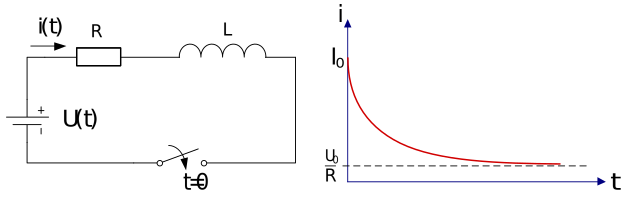
\includegraphics[width=\linewidth]{mai_fig032.pdf}
      \caption{Graf průběhu proudu $i(t)$ po sepnutí spínače v době $t=0$.}
      \label{mai:fig032}
    \end{figure}
%--------------------------------------------------------------------------------------------------- 
%======= Kapitola: Řady funkcí ====================================================================
  % !TeX spellcheck = cs_CZ
%---------------------------------------------------------------------------------------------------
% mai2ch05.tex
%---------------------------------------------------------------------------------------------------
\chapter{Řady funkcí}\label{mai:IIchapV}
\minitoc

%---------------------------------------------------------------------------------------------------
\printbibliography[title={Seznam literatury}, heading=subbibliography]
\addcontentsline{toc}{section}{Seznam literatury}
%======= Kapitola: Závislosti na více parametrech aneb funkce více proměnných =====================
  % !TeX spellcheck = cs_CZ
%---------------------------------------------------------------------------------------------------
% mai2ch06.tex
%---------------------------------------------------------------------------------------------------
\setchaptertoc
\chapter{Závislosti na více parametrech aneb funkce více proměnných}\label{mai:IIchapVI}
  Skalárními funkcemi jedné reálné proměnné jsme se zabývali velmi podrobně v \ref{part:MAI} dílu.
  Umíme počítat jejich limity v bodech \emph{vlastních} i \emph{nevlastních}, umíme je derivovat i
  integrovat. Totéž dokážeme provádět i s vektorovými funkcemi jedné proměnné. Každý vektor je totiž
  dán svými složkami, takže každá vektorová funkce je zadána tolika „obyčejnými“ skalárními
  funkcemi, kolik má daný vektor složek. S vektoroVými funkcemi jedné proměnné jsme pracovali při
  zadávání trajektorií hmotných bodů a výpočtech jejich dalších charakteristik (rychlost, zrychlení,
  křivost trajektorie, apod). Tou jedinou proměnnou byl obvykle čas. Veličiny popisující objekty a
  děje v přírodě, ať již jsou tyto veličiny skaláry či vektory, však většinou závisí na více
  proměnných než jedné. Kromě času bývají typicky závislé na poloze. Vezměme třeba takové gravitační
  pole Země. Na čase sice nezávisí, zato však klesá s druhou mocninou vzdálenosti od středu Země.
  Veličina, která je charakterizuje, je buď vektorová, nebo skalární. Tou vektorovou je
  \emph{gravitační zrychlení} neboli \emph{intenzita} gravitačního pole Země, tou skalární je
  \emph{potenciál},
  \begin{equation*}
    \vec{g}(\vec{r}) = - \kappa\dfrac{M_Z}{r^2}\left(\dfrac{\vec{r}}{r}\right),\,
    V(\vec{r}) = -\kappa\dfrac{M_Z}{r}, \, r\geq R_Z
  \end{equation*}
  V předchozích Vztazích jsou \(M_Z\) a \(R_Z\) hmotnost a poloměr Země, \(\vec{r}\) je polohový
  vektor místa, v němž pole zjištujeme, vzhledem ke středu Země. Skalární i vektorové veličiny
  popisující elektrické a magnetické pole nábojů a proudů, rychlosti elementů proudící kapaliny nebo
  plynu a řada dalších fyzikálních veličin jsou nejen funkcemi času, ale také polohy bodu, v němž je
  počítáme nebo měříme. A stejně jako byly změny funkcí jedné proměnné vyjádřeny pomocí derivací,
  změny změn pomocí druhých derivací, atd., je třeba umět počítat i změny veličin závisejících na
  více proměnných. Mohou samozřejmě nastat situace, kdy se mění jen jedna z proměnných, zatímco
  ostatní zůstávají konstantní. Nejsnáze si takovou situaci představíme například tak, že měříme
  třeba elektrické pole stále ve stejném bodě prostoru, ale běží při tom čas. Pole se v daném bodě s
  časem mění. Nebo naopak v daném okamžiku sledujeme rozdílnost pole v bodech velmi blízkých danému
  bodu. Obecně se samozřejmě mění všechny proměnné a s nimi i hodnoty skalární funkce nebo složky
  vektorové funkce. Jak takové obecné změny co nejvýstižněji popsat, uvidíme právě v této kapitole.
  Setkáme se v ní s \emph{parciální derivací}, která vystihuje, jak rychle se mění hodnota funkce se
  změnou jedné z proměnných. Dále poznáme obecnější, \emph{směrovou derivaci}, která popisuje
  rychlost změny funkční hodnoty, mění-li se všechny proměnné, ale tak, že bod, který reprezentuje
  soubor jejich hodnot, se pohybuje v prostoru proměnných po libovolné přímce (nikoli jen po jedné
  souřadnicové ose, jako tomu je u parciálních derivací). A konečně zavedeme pojmy \emph{úplného
  diferenciálu} a \emph{Jacobiho zobrazení}, které popisují změnu hodnot skalární či vektorové
  funkce v lineární aproximaci, mění-li se hodnoty proměnných zcela obecně.

  Stejně jako u funkcí jedné proměnné je základem pro definici veličin popisujících rychlost změny
  funkce pojem \textbf{limity}, který úzce souvisí s pojmem \emph{okolí bodů} a obecně i s
  definičními obory funkcí. Pro případ funkcí více proměnných klade požadavek hlubšího pochopení
  pojmu limity větší nároky na soustředěnost a důkladné promýšlení různých situací, než tomu bylo u
  limit funkcí jedné proměnné. Proto se jím zabývá podstatná část poměrně rozsáhlého odstavce
  \ref{mai:IIchapVIsecII} poté, co je v odstavci \ref{mai:IIchapVIsecI} věnována značná pozornost
  různým typům definičních oborů funkcí. Čtenář, který se chce rychle propracovat k praktickým
  výpočtům a spokojí se vatím s intuitivním pochopením pojmu limity funkce více proměnných
  (založeným na dobré znalosti definice a vlastností limit funkcí jedné proměnné), může k nim v
  podstatě rovnou přejít s vědomím, že sice bude umět prakticky provádět různé standardní operace s
  funkcemi více proměnných, ale nebude si pravděpodobně vědět rady s netypickými případy. K
  důkladnému pročtení odstavců \ref{mai:IIchapVIsecI} a \ref{mai:IIchapVIsecII} se může samozřejmě
  vrátit kdykoli.

  \section{Podmonožiny euklidovských prostorů \(\mathcal{R}^n\)}\label{mai:IIchapVIsecI}
    S definičními obory funkcí jedné proměnné to bylo docela jednoduché. Byly to Většinou intervaly
    - otevřené intervaly nebo jejich sjednocení, uzavřené intervaly, popřípadě intervaly uzavřené
    jen z jedné strany. Také zde figurovala okolí bodů, ať již ryzí, z nichž byl daný bod vyloučen,
    nebo taková, která daný bod obsahovala. Nic složitého tam nebylo. Aby bylo možné funkce
    derivovat, což byla nejčastější operace, kterou jsme prováděli s cílem zjistit, jak rychle se
    funkce mění, nemohly být definiční obory „moc divoké“. Vždy bylo třeba předpokládat, že bod, v
    němž jsme funkci nebo její změnu vyšetřovali, má okolí, ve kterém je funkce přinejmenším
    definována. Pro případ funkcí více proměnných je to podobné, ale bude třeba se definičním oborům
    věnovat trochu podrobněji. Dejme tomu, že nějaká fyzikální, nebo i nefyzikální veličina bude
    záviset na \(n\) proměnných. Každá z nich může nabývat nějakých hodnot. Funkční hodnota naší
    funkce bude tak jednoznačně určena souborem \(n\) hodnot jednotlivých proměnných. Tuto
    \(n\)-tici budeme považovat za bod v prostoru \(mathcal{R}^n\). S \(n\)-ticemi jsme již
    pracovali v algebře, takže takový popis známe. V algebře jsme však s nimi prováděli algebraické
    operace, sčítání a násobení číslem. Měli jsme tedy v \(mathcal{R}^n\) zavedenou
    \textbf{algebraickou strukturu}. Pro práci s funkcemi a pro sledování jejich změn \uv{bod od bodu}
    potřebujeme v \(mathcal{R}^n\) ještě jinou strukturu. Ta je tvořena okolími, podobně jako tomu
    bylo u funkcí jedné proměnné. Taková struktura se nazývá \emph{topologická} a matematická
    disciplína, která se zabývá topologickými strukturami, se jmenuje \textbf{topologie}.

    Topologickými strukturami se nebudeme zabývat v celé obecnosti, i když je to velmi zajímavé.
    Budeme pracovat pouze se speciálním typem, takzvanou euklidovskou topologtí v \(mathcal{R}^n\).

    \subsection{Okolí bodů, otevřené a uzavřené množiny}
    S pojmem okolí bodu jsme se setkali hned v první části druhé kapitoly prvního dílu. Vzpomínáte?
    Šlo tehdy o okolí bodu \(a\) na reálné ose \(mathcal{R}\). Okolím jsme rozuměli otevřený
    interval \((a - \delta_1,a + \delta_2)\), \(\delta_1, \delta_2 > O\), ryzím okolím pak množinu
    \((a - \delta_1, a + \delta_2)\backslash{a}\), tj. sjednocení otevřených intervalů \((a -
    \delta_1, a) \cup (a, a + \delta_2)\). Sjednocení jakýchkoli otevřených intervalů jsme později
    nazývali otevřenou množinou, doplňky otevřených množin v \(mathcal{R}\) byly uzavřené množiny.
    Vybudovali jsme tak na \(mathcal{R}\) \emph{euklidovskou topologii} (dodatek F prvního dílu).
    Podobná bude situace i ve vícerozměrném případě, tedy v \(mathcal{R}^n\).

  \section{Skalární funkce více proměnných}\label{mai:IIchapVIsecII}
    V předchozím odstavci jsme si vcelku důkladně připravili pojmy týkající se vhodných definičních
    oborů funkcí více proměnných. Nyní budeme tyto funkce definovat a studovat jejich vlastnosti.
    Obdobně jako u funkcí jedné proměnné půjde o limity, spojitost a derivace. Výhoda důkladné
    přípravy pojmů v předchozím odstavci se ukáže již při budování pojmu limity, zejména v
    nevlastním bodě. Samotnému pojmu limity a s ním úzce spjatého pojmu spojitosti bude věnována
    velká pozornost. Někdo se nad tím může pozastavit: Vždyť jak často se s potřebou výpočtu limit
    setkáváme v praktických příkladech? Málo. Potřebujeme spíše derivovat, integrovat, řešit
    diferenciální rovnice. S příklady na limity se setkáváme ponejvíce v matematických sbírkách, kde
    slouží k procvičení naučené látky. Taková úvaha by byla poněkud krátkozraká. Řada vlastností
    funkcí, a vůbec možnost s nimi rozumně operovat při běžných výpočtech, je založena na
    spojitosti. A spojitost je těsně spjata s pojmem limity. Opět by mohla vzniknout námitka, že
    spojitost přece intuitivně dobře chápeme - spojitá funkce nemá „zpřetrhaný“ graf. Umíme si však
    představit graf funkce tří proměnných? Není to dost dobře možné ani u funkce dvou proměnných,
    je-li složitější, nebo chová-li se v okolí některého bodu „podezřelé“. Limitě tedy potřebujeme
    porozumět, i když její výpočet v praktických příkladech skutečně nebude na „denním pořádku“.
    Abychom porozumění podpořili, budeme se vedle teoretických úvah věnovat i řadě praktických
    příkladů.




%---------------------------------------------------------------------------------------------------
%======= Kapitola: Základy variačního počtu pro mechaniku =========================================
  % !TeX spellcheck = cs_CZ
%---------------------------------------------------------------------------------------------------
% mai2ch07.tex
%---------------------------------------------------------------------------------------------------
\setchaptertoc
\chapter{Základy variačního počtu pro mechaniku}\label{mai:IIchapVII}


%---------------------------------------------------------------------------------------------------
}